\documentclass[twoside]{book}

% Packages required by doxygen
\usepackage{calc}
\usepackage{doxygen}
\usepackage{graphicx}
\usepackage[utf8]{inputenc}
\usepackage{makeidx}
\usepackage{multicol}
\usepackage{multirow}
\usepackage{textcomp}
\usepackage[table]{xcolor}

% Font selection
\usepackage[T1]{fontenc}
\usepackage{mathptmx}
\usepackage[scaled=.90]{helvet}
\usepackage{courier}
\usepackage{amssymb}
\usepackage{sectsty}
\renewcommand{\familydefault}{\sfdefault}
\allsectionsfont{%
  \fontseries{bc}\selectfont%
  \color{darkgray}%
}
\renewcommand{\DoxyLabelFont}{%
  \fontseries{bc}\selectfont%
  \color{darkgray}%
}

% Page & text layout
\usepackage{geometry}
\geometry{%
  a4paper,%
  top=2.5cm,%
  bottom=2.5cm,%
  left=2.5cm,%
  right=2.5cm%
}
\tolerance=750
\hfuzz=15pt
\hbadness=750
\setlength{\emergencystretch}{15pt}
\setlength{\parindent}{0cm}
\setlength{\parskip}{0.2cm}
\makeatletter
\renewcommand{\paragraph}{%
  \@startsection{paragraph}{4}{0ex}{-1.0ex}{1.0ex}{%
    \normalfont\normalsize\bfseries\SS@parafont%
  }%
}
\renewcommand{\subparagraph}{%
  \@startsection{subparagraph}{5}{0ex}{-1.0ex}{1.0ex}{%
    \normalfont\normalsize\bfseries\SS@subparafont%
  }%
}
\makeatother

% Headers & footers
\usepackage{fancyhdr}
\pagestyle{fancyplain}
\fancyhead[LE]{\fancyplain{}{\bfseries\thepage}}
\fancyhead[CE]{\fancyplain{}{}}
\fancyhead[RE]{\fancyplain{}{\bfseries\leftmark}}
\fancyhead[LO]{\fancyplain{}{\bfseries\rightmark}}
\fancyhead[CO]{\fancyplain{}{}}
\fancyhead[RO]{\fancyplain{}{\bfseries\thepage}}
\fancyfoot[LE]{\fancyplain{}{}}
\fancyfoot[CE]{\fancyplain{}{}}
\fancyfoot[RE]{\fancyplain{}{\bfseries\scriptsize Generated on Mon Dec 16 2013 10:51:07 for Sudden Awakening by Doxygen }}
\fancyfoot[LO]{\fancyplain{}{\bfseries\scriptsize Generated on Mon Dec 16 2013 10:51:07 for Sudden Awakening by Doxygen }}
\fancyfoot[CO]{\fancyplain{}{}}
\fancyfoot[RO]{\fancyplain{}{}}
\renewcommand{\footrulewidth}{0.4pt}
\renewcommand{\chaptermark}[1]{%
  \markboth{#1}{}%
}
\renewcommand{\sectionmark}[1]{%
  \markright{\thesection\ #1}%
}

% Indices & bibliography
\usepackage{natbib}
\usepackage[titles]{tocloft}
\setcounter{tocdepth}{3}
\setcounter{secnumdepth}{5}
\makeindex

% Hyperlinks (required, but should be loaded last)
\usepackage{ifpdf}
\ifpdf
  \usepackage[pdftex,pagebackref=true]{hyperref}
\else
  \usepackage[ps2pdf,pagebackref=true]{hyperref}
\fi
\hypersetup{%
  colorlinks=true,%
  linkcolor=blue,%
  citecolor=blue,%
  unicode%
}

% Custom commands
\newcommand{\clearemptydoublepage}{%
  \newpage{\pagestyle{empty}\cleardoublepage}%
}


%===== C O N T E N T S =====

\begin{document}

% Titlepage & ToC
\hypersetup{pageanchor=false}
\pagenumbering{roman}
\begin{titlepage}
\vspace*{7cm}
\begin{center}%
{\Large Sudden Awakening }\\
\vspace*{1cm}
{\large Generated by Doxygen 1.8.4}\\
\vspace*{0.5cm}
{\small Mon Dec 16 2013 10:51:07}\\
\end{center}
\end{titlepage}
\clearemptydoublepage
\tableofcontents
\clearemptydoublepage
\pagenumbering{arabic}
\hypersetup{pageanchor=true}

%--- Begin generated contents ---
\chapter{Namespace Index}
\section{Namespace List}
Here is a list of all namespaces with brief descriptions\-:\begin{DoxyCompactList}
\item\contentsline{section}{\hyperlink{namespace_new_state}{New\-State} }{\pageref{namespace_new_state}}{}
\item\contentsline{section}{\hyperlink{namespace_random}{Random} }{\pageref{namespace_random}}{}
\item\contentsline{section}{\hyperlink{namespacesf}{sf} }{\pageref{namespacesf}}{}
\item\contentsline{section}{\hyperlink{namespacetinyxml2}{tinyxml2} }{\pageref{namespacetinyxml2}}{}
\end{DoxyCompactList}

\chapter{Hierarchical Index}
\section{Class Hierarchy}
This inheritance list is sorted roughly, but not completely, alphabetically\-:\begin{DoxyCompactList}
\item \contentsline{section}{Audio\-Effects}{\pageref{class_audio_effects}}{}
\item \contentsline{section}{Button}{\pageref{class_button}}{}
\item \contentsline{section}{Config\-Loader}{\pageref{class_config_loader}}{}
\item \contentsline{section}{tinyxml2\-:\-:Dyn\-Array$<$ T, I\-N\-I\-T $>$}{\pageref{classtinyxml2_1_1_dyn_array}}{}
\item \contentsline{section}{tinyxml2\-:\-:Dyn\-Array$<$ Block $\ast$, 10 $>$}{\pageref{classtinyxml2_1_1_dyn_array}}{}
\item \contentsline{section}{tinyxml2\-:\-:Dyn\-Array$<$ char, 20 $>$}{\pageref{classtinyxml2_1_1_dyn_array}}{}
\item \contentsline{section}{tinyxml2\-:\-:Dyn\-Array$<$ const char $\ast$, 10 $>$}{\pageref{classtinyxml2_1_1_dyn_array}}{}
\item \contentsline{section}{Entity}{\pageref{class_entity}}{}
\begin{DoxyCompactList}
\item \contentsline{section}{Animated\-Entity}{\pageref{class_animated_entity}}{}
\item \contentsline{section}{Map\-Entity}{\pageref{class_map_entity}}{}
\item \contentsline{section}{Player}{\pageref{class_player}}{}
\end{DoxyCompactList}
\item \contentsline{section}{tinyxml2\-:\-:Entity}{\pageref{structtinyxml2_1_1_entity}}{}
\item exception\begin{DoxyCompactList}
\item \contentsline{section}{Runtime\-Exception}{\pageref{class_runtime_exception}}{}
\end{DoxyCompactList}
\item \contentsline{section}{Game}{\pageref{class_game}}{}
\item \contentsline{section}{Level}{\pageref{class_level}}{}
\begin{DoxyCompactList}
\item \contentsline{section}{Level\-One}{\pageref{class_level_one}}{}
\end{DoxyCompactList}
\item \contentsline{section}{Logger}{\pageref{class_logger}}{}
\item \contentsline{section}{tinyxml2\-:\-:Mem\-Pool}{\pageref{classtinyxml2_1_1_mem_pool}}{}
\begin{DoxyCompactList}
\item \contentsline{section}{tinyxml2\-:\-:Mem\-Pool\-T$<$ sizeof(tinyxml2\-:\-:X\-M\-L\-Attribute) $>$}{\pageref{classtinyxml2_1_1_mem_pool_t}}{}
\item \contentsline{section}{tinyxml2\-:\-:Mem\-Pool\-T$<$ sizeof(tinyxml2\-:\-:X\-M\-L\-Comment) $>$}{\pageref{classtinyxml2_1_1_mem_pool_t}}{}
\item \contentsline{section}{tinyxml2\-:\-:Mem\-Pool\-T$<$ sizeof(tinyxml2\-:\-:X\-M\-L\-Element) $>$}{\pageref{classtinyxml2_1_1_mem_pool_t}}{}
\item \contentsline{section}{tinyxml2\-:\-:Mem\-Pool\-T$<$ sizeof(tinyxml2\-:\-:X\-M\-L\-Text) $>$}{\pageref{classtinyxml2_1_1_mem_pool_t}}{}
\item \contentsline{section}{tinyxml2\-:\-:Mem\-Pool\-T$<$ S\-I\-Z\-E $>$}{\pageref{classtinyxml2_1_1_mem_pool_t}}{}
\end{DoxyCompactList}
\item \contentsline{section}{Resource\-Manager$<$ Type $>$}{\pageref{class_resource_manager}}{}
\item \contentsline{section}{Resource\-Manager$<$ sf\-:\-:Texture $>$}{\pageref{class_resource_manager}}{}
\item \contentsline{section}{State}{\pageref{class_state}}{}
\begin{DoxyCompactList}
\item \contentsline{section}{State\-Game\-Play}{\pageref{class_state_game_play}}{}
\item \contentsline{section}{State\-Main\-Menu}{\pageref{class_state_main_menu}}{}
\end{DoxyCompactList}
\item \contentsline{section}{tinyxml2\-:\-:Str\-Pair}{\pageref{classtinyxml2_1_1_str_pair}}{}
\item \contentsline{section}{Tile\-Map}{\pageref{class_tile_map}}{}
\item \contentsline{section}{Tile\-Map\-Layer}{\pageref{class_tile_map_layer}}{}
\item \contentsline{section}{Tile\-Map\-Set}{\pageref{class_tile_map_set}}{}
\item \contentsline{section}{tinyxml2\-:\-:X\-M\-L\-Attribute}{\pageref{classtinyxml2_1_1_x_m_l_attribute}}{}
\item \contentsline{section}{tinyxml2\-:\-:X\-M\-L\-Const\-Handle}{\pageref{classtinyxml2_1_1_x_m_l_const_handle}}{}
\item \contentsline{section}{tinyxml2\-:\-:X\-M\-L\-Handle}{\pageref{classtinyxml2_1_1_x_m_l_handle}}{}
\item \contentsline{section}{tinyxml2\-:\-:X\-M\-L\-Node}{\pageref{classtinyxml2_1_1_x_m_l_node}}{}
\begin{DoxyCompactList}
\item \contentsline{section}{tinyxml2\-:\-:X\-M\-L\-Comment}{\pageref{classtinyxml2_1_1_x_m_l_comment}}{}
\item \contentsline{section}{tinyxml2\-:\-:X\-M\-L\-Declaration}{\pageref{classtinyxml2_1_1_x_m_l_declaration}}{}
\item \contentsline{section}{tinyxml2\-:\-:X\-M\-L\-Document}{\pageref{classtinyxml2_1_1_x_m_l_document}}{}
\item \contentsline{section}{tinyxml2\-:\-:X\-M\-L\-Element}{\pageref{classtinyxml2_1_1_x_m_l_element}}{}
\item \contentsline{section}{tinyxml2\-:\-:X\-M\-L\-Text}{\pageref{classtinyxml2_1_1_x_m_l_text}}{}
\item \contentsline{section}{tinyxml2\-:\-:X\-M\-L\-Unknown}{\pageref{classtinyxml2_1_1_x_m_l_unknown}}{}
\end{DoxyCompactList}
\item \contentsline{section}{tinyxml2\-:\-:X\-M\-L\-Util}{\pageref{classtinyxml2_1_1_x_m_l_util}}{}
\item \contentsline{section}{tinyxml2\-:\-:X\-M\-L\-Visitor}{\pageref{classtinyxml2_1_1_x_m_l_visitor}}{}
\begin{DoxyCompactList}
\item \contentsline{section}{tinyxml2\-:\-:X\-M\-L\-Printer}{\pageref{classtinyxml2_1_1_x_m_l_printer}}{}
\end{DoxyCompactList}
\end{DoxyCompactList}

\chapter{Class Index}
\section{Class List}
Here are the classes, structs, unions and interfaces with brief descriptions\-:\begin{DoxyCompactList}
\item\contentsline{section}{\hyperlink{class_animated_entity}{Animated\-Entity} \\*The \hyperlink{class_animated_entity}{Animated\-Entity} class, unfinished, maybe not used and/or deleted later }{\pageref{class_animated_entity}}{}
\item\contentsline{section}{\hyperlink{class_audio_effects}{Audio\-Effects} \\*The \hyperlink{class_audio_effects}{Audio\-Effects} class }{\pageref{class_audio_effects}}{}
\item\contentsline{section}{\hyperlink{class_button}{Button} \\*The \hyperlink{class_button}{Button} class. This class represents a clickable and selectable button }{\pageref{class_button}}{}
\item\contentsline{section}{\hyperlink{class_config_loader}{Config\-Loader} \\*The \hyperlink{class_config_loader}{Config\-Loader} class, loads it's data from the passed in file and path. The class loads and holds this data temporarily for initialization of the engine. It should only exist durning construction of the engine }{\pageref{class_config_loader}}{}
\item\contentsline{section}{\hyperlink{classtinyxml2_1_1_dyn_array}{tinyxml2\-::\-Dyn\-Array$<$ T, I\-N\-I\-T $>$} }{\pageref{classtinyxml2_1_1_dyn_array}}{}
\item\contentsline{section}{\hyperlink{class_entity}{Entity} \\*The \hyperlink{class_entity}{Entity} class, represents a basic entity that exists in the 2d world }{\pageref{class_entity}}{}
\item\contentsline{section}{\hyperlink{structtinyxml2_1_1_entity}{tinyxml2\-::\-Entity} }{\pageref{structtinyxml2_1_1_entity}}{}
\item\contentsline{section}{\hyperlink{class_game}{Game} \\*Everything for this game starts here }{\pageref{class_game}}{}
\item\contentsline{section}{\hyperlink{class_level}{Level} \\*Everything required to have a level }{\pageref{class_level}}{}
\item\contentsline{section}{\hyperlink{class_level_one}{Level\-One} }{\pageref{class_level_one}}{}
\item\contentsline{section}{\hyperlink{class_logger}{Logger} }{\pageref{class_logger}}{}
\item\contentsline{section}{\hyperlink{class_map_entity}{Map\-Entity} }{\pageref{class_map_entity}}{}
\item\contentsline{section}{\hyperlink{classtinyxml2_1_1_mem_pool}{tinyxml2\-::\-Mem\-Pool} }{\pageref{classtinyxml2_1_1_mem_pool}}{}
\item\contentsline{section}{\hyperlink{classtinyxml2_1_1_mem_pool_t}{tinyxml2\-::\-Mem\-Pool\-T$<$ S\-I\-Z\-E $>$} }{\pageref{classtinyxml2_1_1_mem_pool_t}}{}
\item\contentsline{section}{\hyperlink{class_player}{Player} \\*The \hyperlink{class_player}{Player} class, is the class that holds the data for the player }{\pageref{class_player}}{}
\item\contentsline{section}{\hyperlink{class_resource_manager}{Resource\-Manager$<$ Type $>$} \\*\hyperlink{class_resource_manager}{Resource\-Manager} is simple class for managing resources }{\pageref{class_resource_manager}}{}
\item\contentsline{section}{\hyperlink{class_runtime_exception}{Runtime\-Exception} }{\pageref{class_runtime_exception}}{}
\item\contentsline{section}{\hyperlink{class_state}{State} \\*Base class for states }{\pageref{class_state}}{}
\item\contentsline{section}{\hyperlink{class_state_game_play}{State\-Game\-Play} }{\pageref{class_state_game_play}}{}
\item\contentsline{section}{\hyperlink{class_state_main_menu}{State\-Main\-Menu} }{\pageref{class_state_main_menu}}{}
\item\contentsline{section}{\hyperlink{classtinyxml2_1_1_str_pair}{tinyxml2\-::\-Str\-Pair} }{\pageref{classtinyxml2_1_1_str_pair}}{}
\item\contentsline{section}{\hyperlink{class_tile_map}{Tile\-Map} }{\pageref{class_tile_map}}{}
\item\contentsline{section}{\hyperlink{class_tile_map_layer}{Tile\-Map\-Layer} }{\pageref{class_tile_map_layer}}{}
\item\contentsline{section}{\hyperlink{class_tile_map_set}{Tile\-Map\-Set} }{\pageref{class_tile_map_set}}{}
\item\contentsline{section}{\hyperlink{classtinyxml2_1_1_x_m_l_attribute}{tinyxml2\-::\-X\-M\-L\-Attribute} }{\pageref{classtinyxml2_1_1_x_m_l_attribute}}{}
\item\contentsline{section}{\hyperlink{classtinyxml2_1_1_x_m_l_comment}{tinyxml2\-::\-X\-M\-L\-Comment} }{\pageref{classtinyxml2_1_1_x_m_l_comment}}{}
\item\contentsline{section}{\hyperlink{classtinyxml2_1_1_x_m_l_const_handle}{tinyxml2\-::\-X\-M\-L\-Const\-Handle} }{\pageref{classtinyxml2_1_1_x_m_l_const_handle}}{}
\item\contentsline{section}{\hyperlink{classtinyxml2_1_1_x_m_l_declaration}{tinyxml2\-::\-X\-M\-L\-Declaration} }{\pageref{classtinyxml2_1_1_x_m_l_declaration}}{}
\item\contentsline{section}{\hyperlink{classtinyxml2_1_1_x_m_l_document}{tinyxml2\-::\-X\-M\-L\-Document} }{\pageref{classtinyxml2_1_1_x_m_l_document}}{}
\item\contentsline{section}{\hyperlink{classtinyxml2_1_1_x_m_l_element}{tinyxml2\-::\-X\-M\-L\-Element} }{\pageref{classtinyxml2_1_1_x_m_l_element}}{}
\item\contentsline{section}{\hyperlink{classtinyxml2_1_1_x_m_l_handle}{tinyxml2\-::\-X\-M\-L\-Handle} }{\pageref{classtinyxml2_1_1_x_m_l_handle}}{}
\item\contentsline{section}{\hyperlink{classtinyxml2_1_1_x_m_l_node}{tinyxml2\-::\-X\-M\-L\-Node} }{\pageref{classtinyxml2_1_1_x_m_l_node}}{}
\item\contentsline{section}{\hyperlink{classtinyxml2_1_1_x_m_l_printer}{tinyxml2\-::\-X\-M\-L\-Printer} }{\pageref{classtinyxml2_1_1_x_m_l_printer}}{}
\item\contentsline{section}{\hyperlink{classtinyxml2_1_1_x_m_l_text}{tinyxml2\-::\-X\-M\-L\-Text} }{\pageref{classtinyxml2_1_1_x_m_l_text}}{}
\item\contentsline{section}{\hyperlink{classtinyxml2_1_1_x_m_l_unknown}{tinyxml2\-::\-X\-M\-L\-Unknown} }{\pageref{classtinyxml2_1_1_x_m_l_unknown}}{}
\item\contentsline{section}{\hyperlink{classtinyxml2_1_1_x_m_l_util}{tinyxml2\-::\-X\-M\-L\-Util} }{\pageref{classtinyxml2_1_1_x_m_l_util}}{}
\item\contentsline{section}{\hyperlink{classtinyxml2_1_1_x_m_l_visitor}{tinyxml2\-::\-X\-M\-L\-Visitor} }{\pageref{classtinyxml2_1_1_x_m_l_visitor}}{}
\end{DoxyCompactList}

\chapter{File Index}
\section{File List}
Here is a list of all files with brief descriptions\-:\begin{DoxyCompactList}
\item\contentsline{section}{/home/lee/\-Projects/\-Sudden\-Awakening/\-Source/\hyperlink{_audio_effects_8cpp}{Audio\-Effects.\-cpp} }{\pageref{_audio_effects_8cpp}}{}
\item\contentsline{section}{/home/lee/\-Projects/\-Sudden\-Awakening/\-Source/\hyperlink{_audio_effects_8hpp}{Audio\-Effects.\-hpp} }{\pageref{_audio_effects_8hpp}}{}
\item\contentsline{section}{/home/lee/\-Projects/\-Sudden\-Awakening/\-Source/\hyperlink{_button_8cpp}{Button.\-cpp} }{\pageref{_button_8cpp}}{}
\item\contentsline{section}{/home/lee/\-Projects/\-Sudden\-Awakening/\-Source/\hyperlink{_button_8hpp}{Button.\-hpp} }{\pageref{_button_8hpp}}{}
\item\contentsline{section}{/home/lee/\-Projects/\-Sudden\-Awakening/\-Source/\hyperlink{_config_loader_8cpp}{Config\-Loader.\-cpp} }{\pageref{_config_loader_8cpp}}{}
\item\contentsline{section}{/home/lee/\-Projects/\-Sudden\-Awakening/\-Source/\hyperlink{_config_loader_8hpp}{Config\-Loader.\-hpp} }{\pageref{_config_loader_8hpp}}{}
\item\contentsline{section}{/home/lee/\-Projects/\-Sudden\-Awakening/\-Source/\hyperlink{_entity_8cpp}{Entity.\-cpp} }{\pageref{_entity_8cpp}}{}
\item\contentsline{section}{/home/lee/\-Projects/\-Sudden\-Awakening/\-Source/\hyperlink{_entity_8hpp}{Entity.\-hpp} }{\pageref{_entity_8hpp}}{}
\item\contentsline{section}{/home/lee/\-Projects/\-Sudden\-Awakening/\-Source/\hyperlink{_exceptions_8cpp}{Exceptions.\-cpp} }{\pageref{_exceptions_8cpp}}{}
\item\contentsline{section}{/home/lee/\-Projects/\-Sudden\-Awakening/\-Source/\hyperlink{_exceptions_8hpp}{Exceptions.\-hpp} }{\pageref{_exceptions_8hpp}}{}
\item\contentsline{section}{/home/lee/\-Projects/\-Sudden\-Awakening/\-Source/\hyperlink{_game_8cpp}{Game.\-cpp} }{\pageref{_game_8cpp}}{}
\item\contentsline{section}{/home/lee/\-Projects/\-Sudden\-Awakening/\-Source/\hyperlink{_game_8hpp}{Game.\-hpp} }{\pageref{_game_8hpp}}{}
\item\contentsline{section}{/home/lee/\-Projects/\-Sudden\-Awakening/\-Source/\hyperlink{_level_8cpp}{Level.\-cpp} }{\pageref{_level_8cpp}}{}
\item\contentsline{section}{/home/lee/\-Projects/\-Sudden\-Awakening/\-Source/\hyperlink{_level_8hpp}{Level.\-hpp} }{\pageref{_level_8hpp}}{}
\item\contentsline{section}{/home/lee/\-Projects/\-Sudden\-Awakening/\-Source/\hyperlink{_level_one_8cpp}{Level\-One.\-cpp} }{\pageref{_level_one_8cpp}}{}
\item\contentsline{section}{/home/lee/\-Projects/\-Sudden\-Awakening/\-Source/\hyperlink{_level_one_8hpp}{Level\-One.\-hpp} }{\pageref{_level_one_8hpp}}{}
\item\contentsline{section}{/home/lee/\-Projects/\-Sudden\-Awakening/\-Source/\hyperlink{_logger_8cpp}{Logger.\-cpp} }{\pageref{_logger_8cpp}}{}
\item\contentsline{section}{/home/lee/\-Projects/\-Sudden\-Awakening/\-Source/\hyperlink{_logger_8hpp}{Logger.\-hpp} }{\pageref{_logger_8hpp}}{}
\item\contentsline{section}{/home/lee/\-Projects/\-Sudden\-Awakening/\-Source/\hyperlink{main_8cpp}{main.\-cpp} }{\pageref{main_8cpp}}{}
\item\contentsline{section}{/home/lee/\-Projects/\-Sudden\-Awakening/\-Source/\hyperlink{_random_generator_8cpp}{Random\-Generator.\-cpp} }{\pageref{_random_generator_8cpp}}{}
\item\contentsline{section}{/home/lee/\-Projects/\-Sudden\-Awakening/\-Source/\hyperlink{_random_generator_8hpp}{Random\-Generator.\-hpp} }{\pageref{_random_generator_8hpp}}{}
\item\contentsline{section}{/home/lee/\-Projects/\-Sudden\-Awakening/\-Source/\hyperlink{_resource_manager_8hpp}{Resource\-Manager.\-hpp} }{\pageref{_resource_manager_8hpp}}{}
\item\contentsline{section}{/home/lee/\-Projects/\-Sudden\-Awakening/\-Source/\hyperlink{_state_8cpp}{State.\-cpp} }{\pageref{_state_8cpp}}{}
\item\contentsline{section}{/home/lee/\-Projects/\-Sudden\-Awakening/\-Source/\hyperlink{_state_8hpp}{State.\-hpp} }{\pageref{_state_8hpp}}{}
\item\contentsline{section}{/home/lee/\-Projects/\-Sudden\-Awakening/\-Source/\hyperlink{_state_game_play_8cpp}{State\-Game\-Play.\-cpp} }{\pageref{_state_game_play_8cpp}}{}
\item\contentsline{section}{/home/lee/\-Projects/\-Sudden\-Awakening/\-Source/\hyperlink{_state_game_play_8hpp}{State\-Game\-Play.\-hpp} }{\pageref{_state_game_play_8hpp}}{}
\item\contentsline{section}{/home/lee/\-Projects/\-Sudden\-Awakening/\-Source/\hyperlink{_state_main_menu_8cpp}{State\-Main\-Menu.\-cpp} }{\pageref{_state_main_menu_8cpp}}{}
\item\contentsline{section}{/home/lee/\-Projects/\-Sudden\-Awakening/\-Source/\hyperlink{_state_main_menu_8hpp}{State\-Main\-Menu.\-hpp} }{\pageref{_state_main_menu_8hpp}}{}
\item\contentsline{section}{/home/lee/\-Projects/\-Sudden\-Awakening/\-Source/\hyperlink{_string_utilities_8cpp}{String\-Utilities.\-cpp} }{\pageref{_string_utilities_8cpp}}{}
\item\contentsline{section}{/home/lee/\-Projects/\-Sudden\-Awakening/\-Source/\hyperlink{_string_utilities_8hpp}{String\-Utilities.\-hpp} }{\pageref{_string_utilities_8hpp}}{}
\item\contentsline{section}{/home/lee/\-Projects/\-Sudden\-Awakening/\-Source/\hyperlink{_tile_map_8cpp}{Tile\-Map.\-cpp} }{\pageref{_tile_map_8cpp}}{}
\item\contentsline{section}{/home/lee/\-Projects/\-Sudden\-Awakening/\-Source/\hyperlink{_tile_map_8hpp}{Tile\-Map.\-hpp} }{\pageref{_tile_map_8hpp}}{}
\item\contentsline{section}{/home/lee/\-Projects/\-Sudden\-Awakening/\-Source/\hyperlink{tinyxml2_8cpp}{tinyxml2.\-cpp} }{\pageref{tinyxml2_8cpp}}{}
\item\contentsline{section}{/home/lee/\-Projects/\-Sudden\-Awakening/\-Source/\hyperlink{tinyxml2_8hpp}{tinyxml2.\-hpp} }{\pageref{tinyxml2_8hpp}}{}
\item\contentsline{section}{/home/lee/\-Projects/\-Sudden\-Awakening/\-Source/\hyperlink{_x_m_l_functions_8cpp}{X\-M\-L\-Functions.\-cpp} }{\pageref{_x_m_l_functions_8cpp}}{}
\item\contentsline{section}{/home/lee/\-Projects/\-Sudden\-Awakening/\-Source/\hyperlink{_x_m_l_functions_8hpp}{X\-M\-L\-Functions.\-hpp} }{\pageref{_x_m_l_functions_8hpp}}{}
\end{DoxyCompactList}

\chapter{Namespace Documentation}
\hypertarget{namespace_random}{\section{Random Namespace Reference}
\label{namespace_random}\index{Random@{Random}}
}
\subsection*{Functions}
\begin{DoxyCompactItemize}
\item 
void \hyperlink{namespace_random_a4d271cd065de9fbe8907d4df5bf8f89c}{Seed} ()
\begin{DoxyCompactList}\small\item\em Seed is called to seed the random engines. \end{DoxyCompactList}\item 
float \hyperlink{namespace_random_a9456a1bb9616cb6db26f5452896b2da1}{Between} (float low, float high)
\begin{DoxyCompactList}\small\item\em Between is for getting a random float between two floats. \end{DoxyCompactList}\item 
double \hyperlink{namespace_random_aca0cc9c7b6ac26d4c000fd33e32ef6d9}{Between} (double low, double high)
\begin{DoxyCompactList}\small\item\em Between is for getting a random double between two doubles. \end{DoxyCompactList}\item 
int \hyperlink{namespace_random_a7c53fd9d1c5f259e185d329d8250fee5}{Between} (int low, int high)
\begin{DoxyCompactList}\small\item\em Between is for getting a random in between two ints. \end{DoxyCompactList}\end{DoxyCompactItemize}


\subsection{Function Documentation}
\hypertarget{namespace_random_a9456a1bb9616cb6db26f5452896b2da1}{\index{Random@{Random}!Between@{Between}}
\index{Between@{Between}!Random@{Random}}
\subsubsection[{Between}]{\setlength{\rightskip}{0pt plus 5cm}float Random\-::\-Between (
\begin{DoxyParamCaption}
\item[{float}]{low, }
\item[{float}]{high}
\end{DoxyParamCaption}
)}}\label{namespace_random_a9456a1bb9616cb6db26f5452896b2da1}


Between is for getting a random float between two floats. 


\begin{DoxyParams}{Parameters}
{\em low} & The low side for the range, inclusive. \\
\hline
{\em high} & The high side for the range, inclusive. \\
\hline
\end{DoxyParams}
\begin{DoxyReturn}{Returns}
The random float value. 
\end{DoxyReturn}


Definition at line 19 of file Random\-Generator.\-cpp.

\hypertarget{namespace_random_aca0cc9c7b6ac26d4c000fd33e32ef6d9}{\index{Random@{Random}!Between@{Between}}
\index{Between@{Between}!Random@{Random}}
\subsubsection[{Between}]{\setlength{\rightskip}{0pt plus 5cm}double Random\-::\-Between (
\begin{DoxyParamCaption}
\item[{double}]{low, }
\item[{double}]{high}
\end{DoxyParamCaption}
)}}\label{namespace_random_aca0cc9c7b6ac26d4c000fd33e32ef6d9}


Between is for getting a random double between two doubles. 


\begin{DoxyParams}{Parameters}
{\em low} & The low side for the range, inclusive. \\
\hline
{\em high} & The high side for the range, inclusive. \\
\hline
\end{DoxyParams}
\begin{DoxyReturn}{Returns}
The random double value. 
\end{DoxyReturn}


Definition at line 25 of file Random\-Generator.\-cpp.

\hypertarget{namespace_random_a7c53fd9d1c5f259e185d329d8250fee5}{\index{Random@{Random}!Between@{Between}}
\index{Between@{Between}!Random@{Random}}
\subsubsection[{Between}]{\setlength{\rightskip}{0pt plus 5cm}int Random\-::\-Between (
\begin{DoxyParamCaption}
\item[{int}]{low, }
\item[{int}]{high}
\end{DoxyParamCaption}
)}}\label{namespace_random_a7c53fd9d1c5f259e185d329d8250fee5}


Between is for getting a random in between two ints. 


\begin{DoxyParams}{Parameters}
{\em low} & The low side for the range, inclusive. \\
\hline
{\em high} & The high side for the range, inclusive. \\
\hline
\end{DoxyParams}
\begin{DoxyReturn}{Returns}
The random int value. 
\end{DoxyReturn}


Definition at line 31 of file Random\-Generator.\-cpp.

\hypertarget{namespace_random_a4d271cd065de9fbe8907d4df5bf8f89c}{\index{Random@{Random}!Seed@{Seed}}
\index{Seed@{Seed}!Random@{Random}}
\subsubsection[{Seed}]{\setlength{\rightskip}{0pt plus 5cm}void Random\-::\-Seed (
\begin{DoxyParamCaption}
{}
\end{DoxyParamCaption}
)}}\label{namespace_random_a4d271cd065de9fbe8907d4df5bf8f89c}


Seed is called to seed the random engines. 

Make sure to call this some time early durning engine construction. 

Definition at line 12 of file Random\-Generator.\-cpp.


\hypertarget{namespacesf}{\section{sf Namespace Reference}
\label{namespacesf}\index{sf@{sf}}
}

\hypertarget{namespacetinyxml2}{\section{tinyxml2 Namespace Reference}
\label{namespacetinyxml2}\index{tinyxml2@{tinyxml2}}
}
\subsection*{Classes}
\begin{DoxyCompactItemize}
\item 
struct \hyperlink{structtinyxml2_1_1_entity}{Entity}
\item 
class \hyperlink{classtinyxml2_1_1_str_pair}{Str\-Pair}
\item 
class \hyperlink{classtinyxml2_1_1_dyn_array}{Dyn\-Array}
\item 
class \hyperlink{classtinyxml2_1_1_mem_pool}{Mem\-Pool}
\item 
class \hyperlink{classtinyxml2_1_1_mem_pool_t}{Mem\-Pool\-T}
\item 
class \hyperlink{classtinyxml2_1_1_x_m_l_visitor}{X\-M\-L\-Visitor}
\item 
class \hyperlink{classtinyxml2_1_1_x_m_l_util}{X\-M\-L\-Util}
\item 
class \hyperlink{classtinyxml2_1_1_x_m_l_node}{X\-M\-L\-Node}
\item 
class \hyperlink{classtinyxml2_1_1_x_m_l_text}{X\-M\-L\-Text}
\item 
class \hyperlink{classtinyxml2_1_1_x_m_l_comment}{X\-M\-L\-Comment}
\item 
class \hyperlink{classtinyxml2_1_1_x_m_l_declaration}{X\-M\-L\-Declaration}
\item 
class \hyperlink{classtinyxml2_1_1_x_m_l_unknown}{X\-M\-L\-Unknown}
\item 
class \hyperlink{classtinyxml2_1_1_x_m_l_attribute}{X\-M\-L\-Attribute}
\item 
class \hyperlink{classtinyxml2_1_1_x_m_l_element}{X\-M\-L\-Element}
\item 
class \hyperlink{classtinyxml2_1_1_x_m_l_document}{X\-M\-L\-Document}
\item 
class \hyperlink{classtinyxml2_1_1_x_m_l_handle}{X\-M\-L\-Handle}
\item 
class \hyperlink{classtinyxml2_1_1_x_m_l_const_handle}{X\-M\-L\-Const\-Handle}
\item 
class \hyperlink{classtinyxml2_1_1_x_m_l_printer}{X\-M\-L\-Printer}
\end{DoxyCompactItemize}
\subsection*{Enumerations}
\begin{DoxyCompactItemize}
\item 
enum \hyperlink{namespacetinyxml2_a1fbf88509c3ac88c09117b1947414e08}{X\-M\-L\-Error} \{ \\*
\hyperlink{namespacetinyxml2_a1fbf88509c3ac88c09117b1947414e08ad3b3f200ced09c9fc4166134a4ff8fef}{X\-M\-L\-\_\-\-N\-O\-\_\-\-E\-R\-R\-O\-R} = 0, 
\hyperlink{namespacetinyxml2_a1fbf88509c3ac88c09117b1947414e08a1fe1262fdb5ac05dd9cc4631f8c8e00d}{X\-M\-L\-\_\-\-S\-U\-C\-C\-E\-S\-S} = 0, 
\hyperlink{namespacetinyxml2_a1fbf88509c3ac88c09117b1947414e08abefb89c44285fb68e2218b2c71767f27}{X\-M\-L\-\_\-\-N\-O\-\_\-\-A\-T\-T\-R\-I\-B\-U\-T\-E}, 
\hyperlink{namespacetinyxml2_a1fbf88509c3ac88c09117b1947414e08ae9d8ee545a3a69e90df303257a658113}{X\-M\-L\-\_\-\-W\-R\-O\-N\-G\-\_\-\-A\-T\-T\-R\-I\-B\-U\-T\-E\-\_\-\-T\-Y\-P\-E}, 
\\*
\hyperlink{namespacetinyxml2_a1fbf88509c3ac88c09117b1947414e08a38fd2a97fb1dbebd4c3640d75dc01a94}{X\-M\-L\-\_\-\-E\-R\-R\-O\-R\-\_\-\-F\-I\-L\-E\-\_\-\-N\-O\-T\-\_\-\-F\-O\-U\-N\-D}, 
\hyperlink{namespacetinyxml2_a1fbf88509c3ac88c09117b1947414e08afbbf37655523b79a88b04b77ec0f1258}{X\-M\-L\-\_\-\-E\-R\-R\-O\-R\-\_\-\-F\-I\-L\-E\-\_\-\-C\-O\-U\-L\-D\-\_\-\-N\-O\-T\-\_\-\-B\-E\-\_\-\-O\-P\-E\-N\-E\-D}, 
\hyperlink{namespacetinyxml2_a1fbf88509c3ac88c09117b1947414e08a8d4dd3ce2dee784a53f62fa8a6ac83ee}{X\-M\-L\-\_\-\-E\-R\-R\-O\-R\-\_\-\-F\-I\-L\-E\-\_\-\-R\-E\-A\-D\-\_\-\-E\-R\-R\-O\-R}, 
\hyperlink{namespacetinyxml2_a1fbf88509c3ac88c09117b1947414e08a37759723c0c5e954597654e4eccb4f4d}{X\-M\-L\-\_\-\-E\-R\-R\-O\-R\-\_\-\-E\-L\-E\-M\-E\-N\-T\-\_\-\-M\-I\-S\-M\-A\-T\-C\-H}, 
\\*
\hyperlink{namespacetinyxml2_a1fbf88509c3ac88c09117b1947414e08afa96ea783aa93ea212f9e2d7d3a70ba5}{X\-M\-L\-\_\-\-E\-R\-R\-O\-R\-\_\-\-P\-A\-R\-S\-I\-N\-G\-\_\-\-E\-L\-E\-M\-E\-N\-T}, 
\hyperlink{namespacetinyxml2_a1fbf88509c3ac88c09117b1947414e08a380fd8846799b88773321efae83d26a3}{X\-M\-L\-\_\-\-E\-R\-R\-O\-R\-\_\-\-P\-A\-R\-S\-I\-N\-G\-\_\-\-A\-T\-T\-R\-I\-B\-U\-T\-E}, 
\hyperlink{namespacetinyxml2_a1fbf88509c3ac88c09117b1947414e08a48e646cfca6de90c3770faf535d3ed6b}{X\-M\-L\-\_\-\-E\-R\-R\-O\-R\-\_\-\-I\-D\-E\-N\-T\-I\-F\-Y\-I\-N\-G\-\_\-\-T\-A\-G}, 
\hyperlink{namespacetinyxml2_a1fbf88509c3ac88c09117b1947414e08a50ead30b94c7ae2957b9ccb08ec0994d}{X\-M\-L\-\_\-\-E\-R\-R\-O\-R\-\_\-\-P\-A\-R\-S\-I\-N\-G\-\_\-\-T\-E\-X\-T}, 
\\*
\hyperlink{namespacetinyxml2_a1fbf88509c3ac88c09117b1947414e08a9d181628a1819f2b97835e6bc2c8bb3b}{X\-M\-L\-\_\-\-E\-R\-R\-O\-R\-\_\-\-P\-A\-R\-S\-I\-N\-G\-\_\-\-C\-D\-A\-T\-A}, 
\hyperlink{namespacetinyxml2_a1fbf88509c3ac88c09117b1947414e08a51786809e8b079c770853cf5890a7a35}{X\-M\-L\-\_\-\-E\-R\-R\-O\-R\-\_\-\-P\-A\-R\-S\-I\-N\-G\-\_\-\-C\-O\-M\-M\-E\-N\-T}, 
\hyperlink{namespacetinyxml2_a1fbf88509c3ac88c09117b1947414e08ad45b208578e30dab5a21bff1d8991b87}{X\-M\-L\-\_\-\-E\-R\-R\-O\-R\-\_\-\-P\-A\-R\-S\-I\-N\-G\-\_\-\-D\-E\-C\-L\-A\-R\-A\-T\-I\-O\-N}, 
\hyperlink{namespacetinyxml2_a1fbf88509c3ac88c09117b1947414e08a95a88813812a680fb7372f0149420a97}{X\-M\-L\-\_\-\-E\-R\-R\-O\-R\-\_\-\-P\-A\-R\-S\-I\-N\-G\-\_\-\-U\-N\-K\-N\-O\-W\-N}, 
\\*
\hyperlink{namespacetinyxml2_a1fbf88509c3ac88c09117b1947414e08a1a0478cf44f0a733aa6f21bdf0db80b5}{X\-M\-L\-\_\-\-E\-R\-R\-O\-R\-\_\-\-E\-M\-P\-T\-Y\-\_\-\-D\-O\-C\-U\-M\-E\-N\-T}, 
\hyperlink{namespacetinyxml2_a1fbf88509c3ac88c09117b1947414e08a0cecc816939d9155d33b8a88fd50e4c1}{X\-M\-L\-\_\-\-E\-R\-R\-O\-R\-\_\-\-M\-I\-S\-M\-A\-T\-C\-H\-E\-D\-\_\-\-E\-L\-E\-M\-E\-N\-T}, 
\hyperlink{namespacetinyxml2_a1fbf88509c3ac88c09117b1947414e08af6b4caa10e1f2e9f19a3a24f5f3ce223}{X\-M\-L\-\_\-\-E\-R\-R\-O\-R\-\_\-\-P\-A\-R\-S\-I\-N\-G}, 
\hyperlink{namespacetinyxml2_a1fbf88509c3ac88c09117b1947414e08afdb8840395a7c13dfe6a3e104401c095}{X\-M\-L\-\_\-\-C\-A\-N\-\_\-\-N\-O\-T\-\_\-\-C\-O\-N\-V\-E\-R\-T\-\_\-\-T\-E\-X\-T}, 
\\*
\hyperlink{namespacetinyxml2_a1fbf88509c3ac88c09117b1947414e08a5300bec98feccc8f0cdf567b88821f33}{X\-M\-L\-\_\-\-N\-O\-\_\-\-T\-E\-X\-T\-\_\-\-N\-O\-D\-E}
 \}
\item 
enum \hyperlink{namespacetinyxml2_a7f91d00f77360f850fd5da0861e27dd5}{Whitespace} \{ \hyperlink{namespacetinyxml2_a7f91d00f77360f850fd5da0861e27dd5a751769aa625fe5fe5286e9779edec56a}{P\-R\-E\-S\-E\-R\-V\-E\-\_\-\-W\-H\-I\-T\-E\-S\-P\-A\-C\-E}, 
\hyperlink{namespacetinyxml2_a7f91d00f77360f850fd5da0861e27dd5a9a4a309029a6f5e636e20ef5e0b65136}{C\-O\-L\-L\-A\-P\-S\-E\-\_\-\-W\-H\-I\-T\-E\-S\-P\-A\-C\-E}
 \}
\end{DoxyCompactItemize}


\subsection{Enumeration Type Documentation}
\hypertarget{namespacetinyxml2_a7f91d00f77360f850fd5da0861e27dd5}{\index{tinyxml2@{tinyxml2}!Whitespace@{Whitespace}}
\index{Whitespace@{Whitespace}!tinyxml2@{tinyxml2}}
\subsubsection[{Whitespace}]{\setlength{\rightskip}{0pt plus 5cm}enum {\bf tinyxml2\-::\-Whitespace}}}\label{namespacetinyxml2_a7f91d00f77360f850fd5da0861e27dd5}
\begin{Desc}
\item[Enumerator]\par
\begin{description}
\index{P\-R\-E\-S\-E\-R\-V\-E\-\_\-\-W\-H\-I\-T\-E\-S\-P\-A\-C\-E@{P\-R\-E\-S\-E\-R\-V\-E\-\_\-\-W\-H\-I\-T\-E\-S\-P\-A\-C\-E}!tinyxml2@{tinyxml2}}\index{tinyxml2@{tinyxml2}!P\-R\-E\-S\-E\-R\-V\-E\-\_\-\-W\-H\-I\-T\-E\-S\-P\-A\-C\-E@{P\-R\-E\-S\-E\-R\-V\-E\-\_\-\-W\-H\-I\-T\-E\-S\-P\-A\-C\-E}}\item[{\em 
\hypertarget{namespacetinyxml2_a7f91d00f77360f850fd5da0861e27dd5a751769aa625fe5fe5286e9779edec56a}{P\-R\-E\-S\-E\-R\-V\-E\-\_\-\-W\-H\-I\-T\-E\-S\-P\-A\-C\-E}\label{namespacetinyxml2_a7f91d00f77360f850fd5da0861e27dd5a751769aa625fe5fe5286e9779edec56a}
}]\index{C\-O\-L\-L\-A\-P\-S\-E\-\_\-\-W\-H\-I\-T\-E\-S\-P\-A\-C\-E@{C\-O\-L\-L\-A\-P\-S\-E\-\_\-\-W\-H\-I\-T\-E\-S\-P\-A\-C\-E}!tinyxml2@{tinyxml2}}\index{tinyxml2@{tinyxml2}!C\-O\-L\-L\-A\-P\-S\-E\-\_\-\-W\-H\-I\-T\-E\-S\-P\-A\-C\-E@{C\-O\-L\-L\-A\-P\-S\-E\-\_\-\-W\-H\-I\-T\-E\-S\-P\-A\-C\-E}}\item[{\em 
\hypertarget{namespacetinyxml2_a7f91d00f77360f850fd5da0861e27dd5a9a4a309029a6f5e636e20ef5e0b65136}{C\-O\-L\-L\-A\-P\-S\-E\-\_\-\-W\-H\-I\-T\-E\-S\-P\-A\-C\-E}\label{namespacetinyxml2_a7f91d00f77360f850fd5da0861e27dd5a9a4a309029a6f5e636e20ef5e0b65136}
}]\end{description}
\end{Desc}


Definition at line 1417 of file tinyxml2.\-hpp.

\hypertarget{namespacetinyxml2_a1fbf88509c3ac88c09117b1947414e08}{\index{tinyxml2@{tinyxml2}!X\-M\-L\-Error@{X\-M\-L\-Error}}
\index{X\-M\-L\-Error@{X\-M\-L\-Error}!tinyxml2@{tinyxml2}}
\subsubsection[{X\-M\-L\-Error}]{\setlength{\rightskip}{0pt plus 5cm}enum {\bf tinyxml2\-::\-X\-M\-L\-Error}}}\label{namespacetinyxml2_a1fbf88509c3ac88c09117b1947414e08}
\begin{Desc}
\item[Enumerator]\par
\begin{description}
\index{X\-M\-L\-\_\-\-N\-O\-\_\-\-E\-R\-R\-O\-R@{X\-M\-L\-\_\-\-N\-O\-\_\-\-E\-R\-R\-O\-R}!tinyxml2@{tinyxml2}}\index{tinyxml2@{tinyxml2}!X\-M\-L\-\_\-\-N\-O\-\_\-\-E\-R\-R\-O\-R@{X\-M\-L\-\_\-\-N\-O\-\_\-\-E\-R\-R\-O\-R}}\item[{\em 
\hypertarget{namespacetinyxml2_a1fbf88509c3ac88c09117b1947414e08ad3b3f200ced09c9fc4166134a4ff8fef}{X\-M\-L\-\_\-\-N\-O\-\_\-\-E\-R\-R\-O\-R}\label{namespacetinyxml2_a1fbf88509c3ac88c09117b1947414e08ad3b3f200ced09c9fc4166134a4ff8fef}
}]\index{X\-M\-L\-\_\-\-S\-U\-C\-C\-E\-S\-S@{X\-M\-L\-\_\-\-S\-U\-C\-C\-E\-S\-S}!tinyxml2@{tinyxml2}}\index{tinyxml2@{tinyxml2}!X\-M\-L\-\_\-\-S\-U\-C\-C\-E\-S\-S@{X\-M\-L\-\_\-\-S\-U\-C\-C\-E\-S\-S}}\item[{\em 
\hypertarget{namespacetinyxml2_a1fbf88509c3ac88c09117b1947414e08a1fe1262fdb5ac05dd9cc4631f8c8e00d}{X\-M\-L\-\_\-\-S\-U\-C\-C\-E\-S\-S}\label{namespacetinyxml2_a1fbf88509c3ac88c09117b1947414e08a1fe1262fdb5ac05dd9cc4631f8c8e00d}
}]\index{X\-M\-L\-\_\-\-N\-O\-\_\-\-A\-T\-T\-R\-I\-B\-U\-T\-E@{X\-M\-L\-\_\-\-N\-O\-\_\-\-A\-T\-T\-R\-I\-B\-U\-T\-E}!tinyxml2@{tinyxml2}}\index{tinyxml2@{tinyxml2}!X\-M\-L\-\_\-\-N\-O\-\_\-\-A\-T\-T\-R\-I\-B\-U\-T\-E@{X\-M\-L\-\_\-\-N\-O\-\_\-\-A\-T\-T\-R\-I\-B\-U\-T\-E}}\item[{\em 
\hypertarget{namespacetinyxml2_a1fbf88509c3ac88c09117b1947414e08abefb89c44285fb68e2218b2c71767f27}{X\-M\-L\-\_\-\-N\-O\-\_\-\-A\-T\-T\-R\-I\-B\-U\-T\-E}\label{namespacetinyxml2_a1fbf88509c3ac88c09117b1947414e08abefb89c44285fb68e2218b2c71767f27}
}]\index{X\-M\-L\-\_\-\-W\-R\-O\-N\-G\-\_\-\-A\-T\-T\-R\-I\-B\-U\-T\-E\-\_\-\-T\-Y\-P\-E@{X\-M\-L\-\_\-\-W\-R\-O\-N\-G\-\_\-\-A\-T\-T\-R\-I\-B\-U\-T\-E\-\_\-\-T\-Y\-P\-E}!tinyxml2@{tinyxml2}}\index{tinyxml2@{tinyxml2}!X\-M\-L\-\_\-\-W\-R\-O\-N\-G\-\_\-\-A\-T\-T\-R\-I\-B\-U\-T\-E\-\_\-\-T\-Y\-P\-E@{X\-M\-L\-\_\-\-W\-R\-O\-N\-G\-\_\-\-A\-T\-T\-R\-I\-B\-U\-T\-E\-\_\-\-T\-Y\-P\-E}}\item[{\em 
\hypertarget{namespacetinyxml2_a1fbf88509c3ac88c09117b1947414e08ae9d8ee545a3a69e90df303257a658113}{X\-M\-L\-\_\-\-W\-R\-O\-N\-G\-\_\-\-A\-T\-T\-R\-I\-B\-U\-T\-E\-\_\-\-T\-Y\-P\-E}\label{namespacetinyxml2_a1fbf88509c3ac88c09117b1947414e08ae9d8ee545a3a69e90df303257a658113}
}]\index{X\-M\-L\-\_\-\-E\-R\-R\-O\-R\-\_\-\-F\-I\-L\-E\-\_\-\-N\-O\-T\-\_\-\-F\-O\-U\-N\-D@{X\-M\-L\-\_\-\-E\-R\-R\-O\-R\-\_\-\-F\-I\-L\-E\-\_\-\-N\-O\-T\-\_\-\-F\-O\-U\-N\-D}!tinyxml2@{tinyxml2}}\index{tinyxml2@{tinyxml2}!X\-M\-L\-\_\-\-E\-R\-R\-O\-R\-\_\-\-F\-I\-L\-E\-\_\-\-N\-O\-T\-\_\-\-F\-O\-U\-N\-D@{X\-M\-L\-\_\-\-E\-R\-R\-O\-R\-\_\-\-F\-I\-L\-E\-\_\-\-N\-O\-T\-\_\-\-F\-O\-U\-N\-D}}\item[{\em 
\hypertarget{namespacetinyxml2_a1fbf88509c3ac88c09117b1947414e08a38fd2a97fb1dbebd4c3640d75dc01a94}{X\-M\-L\-\_\-\-E\-R\-R\-O\-R\-\_\-\-F\-I\-L\-E\-\_\-\-N\-O\-T\-\_\-\-F\-O\-U\-N\-D}\label{namespacetinyxml2_a1fbf88509c3ac88c09117b1947414e08a38fd2a97fb1dbebd4c3640d75dc01a94}
}]\index{X\-M\-L\-\_\-\-E\-R\-R\-O\-R\-\_\-\-F\-I\-L\-E\-\_\-\-C\-O\-U\-L\-D\-\_\-\-N\-O\-T\-\_\-\-B\-E\-\_\-\-O\-P\-E\-N\-E\-D@{X\-M\-L\-\_\-\-E\-R\-R\-O\-R\-\_\-\-F\-I\-L\-E\-\_\-\-C\-O\-U\-L\-D\-\_\-\-N\-O\-T\-\_\-\-B\-E\-\_\-\-O\-P\-E\-N\-E\-D}!tinyxml2@{tinyxml2}}\index{tinyxml2@{tinyxml2}!X\-M\-L\-\_\-\-E\-R\-R\-O\-R\-\_\-\-F\-I\-L\-E\-\_\-\-C\-O\-U\-L\-D\-\_\-\-N\-O\-T\-\_\-\-B\-E\-\_\-\-O\-P\-E\-N\-E\-D@{X\-M\-L\-\_\-\-E\-R\-R\-O\-R\-\_\-\-F\-I\-L\-E\-\_\-\-C\-O\-U\-L\-D\-\_\-\-N\-O\-T\-\_\-\-B\-E\-\_\-\-O\-P\-E\-N\-E\-D}}\item[{\em 
\hypertarget{namespacetinyxml2_a1fbf88509c3ac88c09117b1947414e08afbbf37655523b79a88b04b77ec0f1258}{X\-M\-L\-\_\-\-E\-R\-R\-O\-R\-\_\-\-F\-I\-L\-E\-\_\-\-C\-O\-U\-L\-D\-\_\-\-N\-O\-T\-\_\-\-B\-E\-\_\-\-O\-P\-E\-N\-E\-D}\label{namespacetinyxml2_a1fbf88509c3ac88c09117b1947414e08afbbf37655523b79a88b04b77ec0f1258}
}]\index{X\-M\-L\-\_\-\-E\-R\-R\-O\-R\-\_\-\-F\-I\-L\-E\-\_\-\-R\-E\-A\-D\-\_\-\-E\-R\-R\-O\-R@{X\-M\-L\-\_\-\-E\-R\-R\-O\-R\-\_\-\-F\-I\-L\-E\-\_\-\-R\-E\-A\-D\-\_\-\-E\-R\-R\-O\-R}!tinyxml2@{tinyxml2}}\index{tinyxml2@{tinyxml2}!X\-M\-L\-\_\-\-E\-R\-R\-O\-R\-\_\-\-F\-I\-L\-E\-\_\-\-R\-E\-A\-D\-\_\-\-E\-R\-R\-O\-R@{X\-M\-L\-\_\-\-E\-R\-R\-O\-R\-\_\-\-F\-I\-L\-E\-\_\-\-R\-E\-A\-D\-\_\-\-E\-R\-R\-O\-R}}\item[{\em 
\hypertarget{namespacetinyxml2_a1fbf88509c3ac88c09117b1947414e08a8d4dd3ce2dee784a53f62fa8a6ac83ee}{X\-M\-L\-\_\-\-E\-R\-R\-O\-R\-\_\-\-F\-I\-L\-E\-\_\-\-R\-E\-A\-D\-\_\-\-E\-R\-R\-O\-R}\label{namespacetinyxml2_a1fbf88509c3ac88c09117b1947414e08a8d4dd3ce2dee784a53f62fa8a6ac83ee}
}]\index{X\-M\-L\-\_\-\-E\-R\-R\-O\-R\-\_\-\-E\-L\-E\-M\-E\-N\-T\-\_\-\-M\-I\-S\-M\-A\-T\-C\-H@{X\-M\-L\-\_\-\-E\-R\-R\-O\-R\-\_\-\-E\-L\-E\-M\-E\-N\-T\-\_\-\-M\-I\-S\-M\-A\-T\-C\-H}!tinyxml2@{tinyxml2}}\index{tinyxml2@{tinyxml2}!X\-M\-L\-\_\-\-E\-R\-R\-O\-R\-\_\-\-E\-L\-E\-M\-E\-N\-T\-\_\-\-M\-I\-S\-M\-A\-T\-C\-H@{X\-M\-L\-\_\-\-E\-R\-R\-O\-R\-\_\-\-E\-L\-E\-M\-E\-N\-T\-\_\-\-M\-I\-S\-M\-A\-T\-C\-H}}\item[{\em 
\hypertarget{namespacetinyxml2_a1fbf88509c3ac88c09117b1947414e08a37759723c0c5e954597654e4eccb4f4d}{X\-M\-L\-\_\-\-E\-R\-R\-O\-R\-\_\-\-E\-L\-E\-M\-E\-N\-T\-\_\-\-M\-I\-S\-M\-A\-T\-C\-H}\label{namespacetinyxml2_a1fbf88509c3ac88c09117b1947414e08a37759723c0c5e954597654e4eccb4f4d}
}]\index{X\-M\-L\-\_\-\-E\-R\-R\-O\-R\-\_\-\-P\-A\-R\-S\-I\-N\-G\-\_\-\-E\-L\-E\-M\-E\-N\-T@{X\-M\-L\-\_\-\-E\-R\-R\-O\-R\-\_\-\-P\-A\-R\-S\-I\-N\-G\-\_\-\-E\-L\-E\-M\-E\-N\-T}!tinyxml2@{tinyxml2}}\index{tinyxml2@{tinyxml2}!X\-M\-L\-\_\-\-E\-R\-R\-O\-R\-\_\-\-P\-A\-R\-S\-I\-N\-G\-\_\-\-E\-L\-E\-M\-E\-N\-T@{X\-M\-L\-\_\-\-E\-R\-R\-O\-R\-\_\-\-P\-A\-R\-S\-I\-N\-G\-\_\-\-E\-L\-E\-M\-E\-N\-T}}\item[{\em 
\hypertarget{namespacetinyxml2_a1fbf88509c3ac88c09117b1947414e08afa96ea783aa93ea212f9e2d7d3a70ba5}{X\-M\-L\-\_\-\-E\-R\-R\-O\-R\-\_\-\-P\-A\-R\-S\-I\-N\-G\-\_\-\-E\-L\-E\-M\-E\-N\-T}\label{namespacetinyxml2_a1fbf88509c3ac88c09117b1947414e08afa96ea783aa93ea212f9e2d7d3a70ba5}
}]\index{X\-M\-L\-\_\-\-E\-R\-R\-O\-R\-\_\-\-P\-A\-R\-S\-I\-N\-G\-\_\-\-A\-T\-T\-R\-I\-B\-U\-T\-E@{X\-M\-L\-\_\-\-E\-R\-R\-O\-R\-\_\-\-P\-A\-R\-S\-I\-N\-G\-\_\-\-A\-T\-T\-R\-I\-B\-U\-T\-E}!tinyxml2@{tinyxml2}}\index{tinyxml2@{tinyxml2}!X\-M\-L\-\_\-\-E\-R\-R\-O\-R\-\_\-\-P\-A\-R\-S\-I\-N\-G\-\_\-\-A\-T\-T\-R\-I\-B\-U\-T\-E@{X\-M\-L\-\_\-\-E\-R\-R\-O\-R\-\_\-\-P\-A\-R\-S\-I\-N\-G\-\_\-\-A\-T\-T\-R\-I\-B\-U\-T\-E}}\item[{\em 
\hypertarget{namespacetinyxml2_a1fbf88509c3ac88c09117b1947414e08a380fd8846799b88773321efae83d26a3}{X\-M\-L\-\_\-\-E\-R\-R\-O\-R\-\_\-\-P\-A\-R\-S\-I\-N\-G\-\_\-\-A\-T\-T\-R\-I\-B\-U\-T\-E}\label{namespacetinyxml2_a1fbf88509c3ac88c09117b1947414e08a380fd8846799b88773321efae83d26a3}
}]\index{X\-M\-L\-\_\-\-E\-R\-R\-O\-R\-\_\-\-I\-D\-E\-N\-T\-I\-F\-Y\-I\-N\-G\-\_\-\-T\-A\-G@{X\-M\-L\-\_\-\-E\-R\-R\-O\-R\-\_\-\-I\-D\-E\-N\-T\-I\-F\-Y\-I\-N\-G\-\_\-\-T\-A\-G}!tinyxml2@{tinyxml2}}\index{tinyxml2@{tinyxml2}!X\-M\-L\-\_\-\-E\-R\-R\-O\-R\-\_\-\-I\-D\-E\-N\-T\-I\-F\-Y\-I\-N\-G\-\_\-\-T\-A\-G@{X\-M\-L\-\_\-\-E\-R\-R\-O\-R\-\_\-\-I\-D\-E\-N\-T\-I\-F\-Y\-I\-N\-G\-\_\-\-T\-A\-G}}\item[{\em 
\hypertarget{namespacetinyxml2_a1fbf88509c3ac88c09117b1947414e08a48e646cfca6de90c3770faf535d3ed6b}{X\-M\-L\-\_\-\-E\-R\-R\-O\-R\-\_\-\-I\-D\-E\-N\-T\-I\-F\-Y\-I\-N\-G\-\_\-\-T\-A\-G}\label{namespacetinyxml2_a1fbf88509c3ac88c09117b1947414e08a48e646cfca6de90c3770faf535d3ed6b}
}]\index{X\-M\-L\-\_\-\-E\-R\-R\-O\-R\-\_\-\-P\-A\-R\-S\-I\-N\-G\-\_\-\-T\-E\-X\-T@{X\-M\-L\-\_\-\-E\-R\-R\-O\-R\-\_\-\-P\-A\-R\-S\-I\-N\-G\-\_\-\-T\-E\-X\-T}!tinyxml2@{tinyxml2}}\index{tinyxml2@{tinyxml2}!X\-M\-L\-\_\-\-E\-R\-R\-O\-R\-\_\-\-P\-A\-R\-S\-I\-N\-G\-\_\-\-T\-E\-X\-T@{X\-M\-L\-\_\-\-E\-R\-R\-O\-R\-\_\-\-P\-A\-R\-S\-I\-N\-G\-\_\-\-T\-E\-X\-T}}\item[{\em 
\hypertarget{namespacetinyxml2_a1fbf88509c3ac88c09117b1947414e08a50ead30b94c7ae2957b9ccb08ec0994d}{X\-M\-L\-\_\-\-E\-R\-R\-O\-R\-\_\-\-P\-A\-R\-S\-I\-N\-G\-\_\-\-T\-E\-X\-T}\label{namespacetinyxml2_a1fbf88509c3ac88c09117b1947414e08a50ead30b94c7ae2957b9ccb08ec0994d}
}]\index{X\-M\-L\-\_\-\-E\-R\-R\-O\-R\-\_\-\-P\-A\-R\-S\-I\-N\-G\-\_\-\-C\-D\-A\-T\-A@{X\-M\-L\-\_\-\-E\-R\-R\-O\-R\-\_\-\-P\-A\-R\-S\-I\-N\-G\-\_\-\-C\-D\-A\-T\-A}!tinyxml2@{tinyxml2}}\index{tinyxml2@{tinyxml2}!X\-M\-L\-\_\-\-E\-R\-R\-O\-R\-\_\-\-P\-A\-R\-S\-I\-N\-G\-\_\-\-C\-D\-A\-T\-A@{X\-M\-L\-\_\-\-E\-R\-R\-O\-R\-\_\-\-P\-A\-R\-S\-I\-N\-G\-\_\-\-C\-D\-A\-T\-A}}\item[{\em 
\hypertarget{namespacetinyxml2_a1fbf88509c3ac88c09117b1947414e08a9d181628a1819f2b97835e6bc2c8bb3b}{X\-M\-L\-\_\-\-E\-R\-R\-O\-R\-\_\-\-P\-A\-R\-S\-I\-N\-G\-\_\-\-C\-D\-A\-T\-A}\label{namespacetinyxml2_a1fbf88509c3ac88c09117b1947414e08a9d181628a1819f2b97835e6bc2c8bb3b}
}]\index{X\-M\-L\-\_\-\-E\-R\-R\-O\-R\-\_\-\-P\-A\-R\-S\-I\-N\-G\-\_\-\-C\-O\-M\-M\-E\-N\-T@{X\-M\-L\-\_\-\-E\-R\-R\-O\-R\-\_\-\-P\-A\-R\-S\-I\-N\-G\-\_\-\-C\-O\-M\-M\-E\-N\-T}!tinyxml2@{tinyxml2}}\index{tinyxml2@{tinyxml2}!X\-M\-L\-\_\-\-E\-R\-R\-O\-R\-\_\-\-P\-A\-R\-S\-I\-N\-G\-\_\-\-C\-O\-M\-M\-E\-N\-T@{X\-M\-L\-\_\-\-E\-R\-R\-O\-R\-\_\-\-P\-A\-R\-S\-I\-N\-G\-\_\-\-C\-O\-M\-M\-E\-N\-T}}\item[{\em 
\hypertarget{namespacetinyxml2_a1fbf88509c3ac88c09117b1947414e08a51786809e8b079c770853cf5890a7a35}{X\-M\-L\-\_\-\-E\-R\-R\-O\-R\-\_\-\-P\-A\-R\-S\-I\-N\-G\-\_\-\-C\-O\-M\-M\-E\-N\-T}\label{namespacetinyxml2_a1fbf88509c3ac88c09117b1947414e08a51786809e8b079c770853cf5890a7a35}
}]\index{X\-M\-L\-\_\-\-E\-R\-R\-O\-R\-\_\-\-P\-A\-R\-S\-I\-N\-G\-\_\-\-D\-E\-C\-L\-A\-R\-A\-T\-I\-O\-N@{X\-M\-L\-\_\-\-E\-R\-R\-O\-R\-\_\-\-P\-A\-R\-S\-I\-N\-G\-\_\-\-D\-E\-C\-L\-A\-R\-A\-T\-I\-O\-N}!tinyxml2@{tinyxml2}}\index{tinyxml2@{tinyxml2}!X\-M\-L\-\_\-\-E\-R\-R\-O\-R\-\_\-\-P\-A\-R\-S\-I\-N\-G\-\_\-\-D\-E\-C\-L\-A\-R\-A\-T\-I\-O\-N@{X\-M\-L\-\_\-\-E\-R\-R\-O\-R\-\_\-\-P\-A\-R\-S\-I\-N\-G\-\_\-\-D\-E\-C\-L\-A\-R\-A\-T\-I\-O\-N}}\item[{\em 
\hypertarget{namespacetinyxml2_a1fbf88509c3ac88c09117b1947414e08ad45b208578e30dab5a21bff1d8991b87}{X\-M\-L\-\_\-\-E\-R\-R\-O\-R\-\_\-\-P\-A\-R\-S\-I\-N\-G\-\_\-\-D\-E\-C\-L\-A\-R\-A\-T\-I\-O\-N}\label{namespacetinyxml2_a1fbf88509c3ac88c09117b1947414e08ad45b208578e30dab5a21bff1d8991b87}
}]\index{X\-M\-L\-\_\-\-E\-R\-R\-O\-R\-\_\-\-P\-A\-R\-S\-I\-N\-G\-\_\-\-U\-N\-K\-N\-O\-W\-N@{X\-M\-L\-\_\-\-E\-R\-R\-O\-R\-\_\-\-P\-A\-R\-S\-I\-N\-G\-\_\-\-U\-N\-K\-N\-O\-W\-N}!tinyxml2@{tinyxml2}}\index{tinyxml2@{tinyxml2}!X\-M\-L\-\_\-\-E\-R\-R\-O\-R\-\_\-\-P\-A\-R\-S\-I\-N\-G\-\_\-\-U\-N\-K\-N\-O\-W\-N@{X\-M\-L\-\_\-\-E\-R\-R\-O\-R\-\_\-\-P\-A\-R\-S\-I\-N\-G\-\_\-\-U\-N\-K\-N\-O\-W\-N}}\item[{\em 
\hypertarget{namespacetinyxml2_a1fbf88509c3ac88c09117b1947414e08a95a88813812a680fb7372f0149420a97}{X\-M\-L\-\_\-\-E\-R\-R\-O\-R\-\_\-\-P\-A\-R\-S\-I\-N\-G\-\_\-\-U\-N\-K\-N\-O\-W\-N}\label{namespacetinyxml2_a1fbf88509c3ac88c09117b1947414e08a95a88813812a680fb7372f0149420a97}
}]\index{X\-M\-L\-\_\-\-E\-R\-R\-O\-R\-\_\-\-E\-M\-P\-T\-Y\-\_\-\-D\-O\-C\-U\-M\-E\-N\-T@{X\-M\-L\-\_\-\-E\-R\-R\-O\-R\-\_\-\-E\-M\-P\-T\-Y\-\_\-\-D\-O\-C\-U\-M\-E\-N\-T}!tinyxml2@{tinyxml2}}\index{tinyxml2@{tinyxml2}!X\-M\-L\-\_\-\-E\-R\-R\-O\-R\-\_\-\-E\-M\-P\-T\-Y\-\_\-\-D\-O\-C\-U\-M\-E\-N\-T@{X\-M\-L\-\_\-\-E\-R\-R\-O\-R\-\_\-\-E\-M\-P\-T\-Y\-\_\-\-D\-O\-C\-U\-M\-E\-N\-T}}\item[{\em 
\hypertarget{namespacetinyxml2_a1fbf88509c3ac88c09117b1947414e08a1a0478cf44f0a733aa6f21bdf0db80b5}{X\-M\-L\-\_\-\-E\-R\-R\-O\-R\-\_\-\-E\-M\-P\-T\-Y\-\_\-\-D\-O\-C\-U\-M\-E\-N\-T}\label{namespacetinyxml2_a1fbf88509c3ac88c09117b1947414e08a1a0478cf44f0a733aa6f21bdf0db80b5}
}]\index{X\-M\-L\-\_\-\-E\-R\-R\-O\-R\-\_\-\-M\-I\-S\-M\-A\-T\-C\-H\-E\-D\-\_\-\-E\-L\-E\-M\-E\-N\-T@{X\-M\-L\-\_\-\-E\-R\-R\-O\-R\-\_\-\-M\-I\-S\-M\-A\-T\-C\-H\-E\-D\-\_\-\-E\-L\-E\-M\-E\-N\-T}!tinyxml2@{tinyxml2}}\index{tinyxml2@{tinyxml2}!X\-M\-L\-\_\-\-E\-R\-R\-O\-R\-\_\-\-M\-I\-S\-M\-A\-T\-C\-H\-E\-D\-\_\-\-E\-L\-E\-M\-E\-N\-T@{X\-M\-L\-\_\-\-E\-R\-R\-O\-R\-\_\-\-M\-I\-S\-M\-A\-T\-C\-H\-E\-D\-\_\-\-E\-L\-E\-M\-E\-N\-T}}\item[{\em 
\hypertarget{namespacetinyxml2_a1fbf88509c3ac88c09117b1947414e08a0cecc816939d9155d33b8a88fd50e4c1}{X\-M\-L\-\_\-\-E\-R\-R\-O\-R\-\_\-\-M\-I\-S\-M\-A\-T\-C\-H\-E\-D\-\_\-\-E\-L\-E\-M\-E\-N\-T}\label{namespacetinyxml2_a1fbf88509c3ac88c09117b1947414e08a0cecc816939d9155d33b8a88fd50e4c1}
}]\index{X\-M\-L\-\_\-\-E\-R\-R\-O\-R\-\_\-\-P\-A\-R\-S\-I\-N\-G@{X\-M\-L\-\_\-\-E\-R\-R\-O\-R\-\_\-\-P\-A\-R\-S\-I\-N\-G}!tinyxml2@{tinyxml2}}\index{tinyxml2@{tinyxml2}!X\-M\-L\-\_\-\-E\-R\-R\-O\-R\-\_\-\-P\-A\-R\-S\-I\-N\-G@{X\-M\-L\-\_\-\-E\-R\-R\-O\-R\-\_\-\-P\-A\-R\-S\-I\-N\-G}}\item[{\em 
\hypertarget{namespacetinyxml2_a1fbf88509c3ac88c09117b1947414e08af6b4caa10e1f2e9f19a3a24f5f3ce223}{X\-M\-L\-\_\-\-E\-R\-R\-O\-R\-\_\-\-P\-A\-R\-S\-I\-N\-G}\label{namespacetinyxml2_a1fbf88509c3ac88c09117b1947414e08af6b4caa10e1f2e9f19a3a24f5f3ce223}
}]\index{X\-M\-L\-\_\-\-C\-A\-N\-\_\-\-N\-O\-T\-\_\-\-C\-O\-N\-V\-E\-R\-T\-\_\-\-T\-E\-X\-T@{X\-M\-L\-\_\-\-C\-A\-N\-\_\-\-N\-O\-T\-\_\-\-C\-O\-N\-V\-E\-R\-T\-\_\-\-T\-E\-X\-T}!tinyxml2@{tinyxml2}}\index{tinyxml2@{tinyxml2}!X\-M\-L\-\_\-\-C\-A\-N\-\_\-\-N\-O\-T\-\_\-\-C\-O\-N\-V\-E\-R\-T\-\_\-\-T\-E\-X\-T@{X\-M\-L\-\_\-\-C\-A\-N\-\_\-\-N\-O\-T\-\_\-\-C\-O\-N\-V\-E\-R\-T\-\_\-\-T\-E\-X\-T}}\item[{\em 
\hypertarget{namespacetinyxml2_a1fbf88509c3ac88c09117b1947414e08afdb8840395a7c13dfe6a3e104401c095}{X\-M\-L\-\_\-\-C\-A\-N\-\_\-\-N\-O\-T\-\_\-\-C\-O\-N\-V\-E\-R\-T\-\_\-\-T\-E\-X\-T}\label{namespacetinyxml2_a1fbf88509c3ac88c09117b1947414e08afdb8840395a7c13dfe6a3e104401c095}
}]\index{X\-M\-L\-\_\-\-N\-O\-\_\-\-T\-E\-X\-T\-\_\-\-N\-O\-D\-E@{X\-M\-L\-\_\-\-N\-O\-\_\-\-T\-E\-X\-T\-\_\-\-N\-O\-D\-E}!tinyxml2@{tinyxml2}}\index{tinyxml2@{tinyxml2}!X\-M\-L\-\_\-\-N\-O\-\_\-\-T\-E\-X\-T\-\_\-\-N\-O\-D\-E@{X\-M\-L\-\_\-\-N\-O\-\_\-\-T\-E\-X\-T\-\_\-\-N\-O\-D\-E}}\item[{\em 
\hypertarget{namespacetinyxml2_a1fbf88509c3ac88c09117b1947414e08a5300bec98feccc8f0cdf567b88821f33}{X\-M\-L\-\_\-\-N\-O\-\_\-\-T\-E\-X\-T\-\_\-\-N\-O\-D\-E}\label{namespacetinyxml2_a1fbf88509c3ac88c09117b1947414e08a5300bec98feccc8f0cdf567b88821f33}
}]\end{description}
\end{Desc}


Definition at line 973 of file tinyxml2.\-hpp.


\chapter{Class Documentation}
\hypertarget{class_animated_entity}{\section{Animated\-Entity Class Reference}
\label{class_animated_entity}\index{Animated\-Entity@{Animated\-Entity}}
}


The \hyperlink{class_animated_entity}{Animated\-Entity} class, unfinished, maybe not used and/or deleted later.  




{\ttfamily \#include $<$Entity.\-hpp$>$}

Inheritance diagram for Animated\-Entity\-:\begin{figure}[H]
\begin{center}
\leavevmode
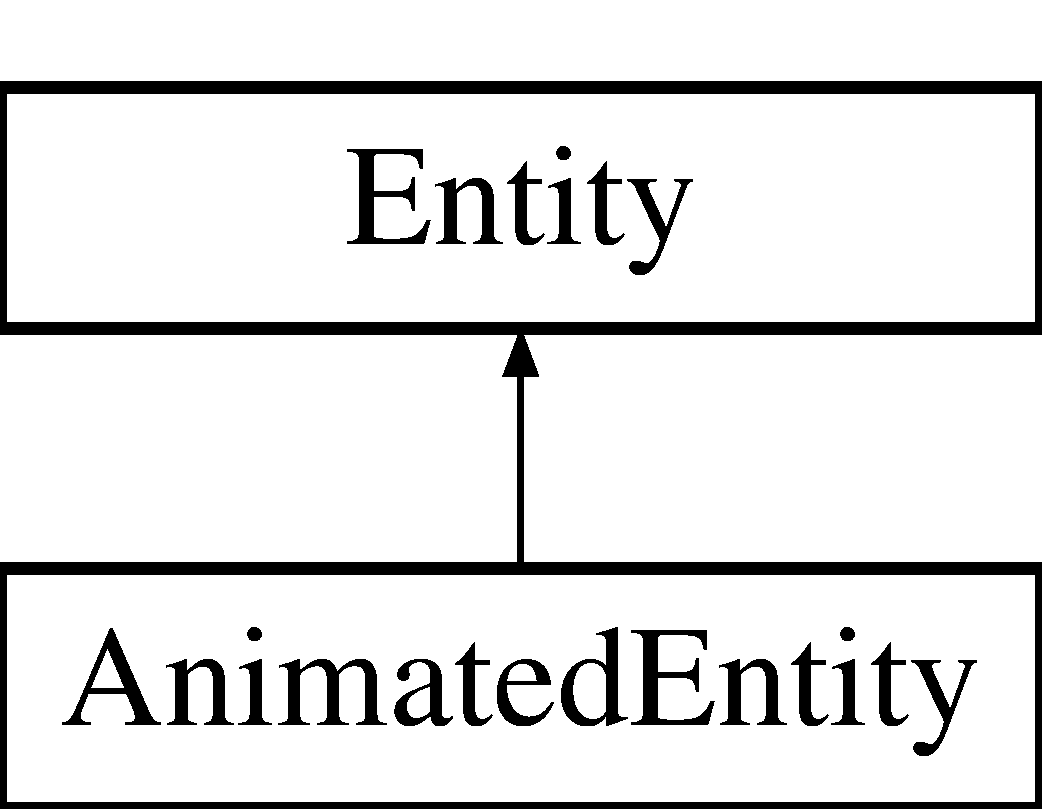
\includegraphics[height=2.000000cm]{class_animated_entity}
\end{center}
\end{figure}
\subsection*{Public Member Functions}
\begin{DoxyCompactItemize}
\item 
\hyperlink{class_animated_entity_af4dfa59419bc469aa24607979e48ba5d}{Animated\-Entity} (const sf\-::\-Texture \&texture, const sf\-::\-Vector2f \&pos)
\item 
virtual \hyperlink{class_animated_entity_a11bb45960aebeed89cf0f8cd3aec4ea2}{$\sim$\-Animated\-Entity} ()
\item 
virtual void \hyperlink{class_animated_entity_af12d83ab3604a110e37c66c33206104b}{Update} ()
\begin{DoxyCompactList}\small\item\em Update virtual call to update entities, and their child class. \end{DoxyCompactList}\end{DoxyCompactItemize}
\subsection*{Additional Inherited Members}


\subsection{Detailed Description}
The \hyperlink{class_animated_entity}{Animated\-Entity} class, unfinished, maybe not used and/or deleted later. 

Definition at line 109 of file Entity.\-hpp.



\subsection{Constructor \& Destructor Documentation}
\hypertarget{class_animated_entity_af4dfa59419bc469aa24607979e48ba5d}{\index{Animated\-Entity@{Animated\-Entity}!Animated\-Entity@{Animated\-Entity}}
\index{Animated\-Entity@{Animated\-Entity}!AnimatedEntity@{Animated\-Entity}}
\subsubsection[{Animated\-Entity}]{\setlength{\rightskip}{0pt plus 5cm}Animated\-Entity\-::\-Animated\-Entity (
\begin{DoxyParamCaption}
\item[{const sf\-::\-Texture \&}]{texture, }
\item[{const sf\-::\-Vector2f \&}]{pos}
\end{DoxyParamCaption}
)}}\label{class_animated_entity_af4dfa59419bc469aa24607979e48ba5d}


Definition at line 73 of file Entity.\-cpp.

\hypertarget{class_animated_entity_a11bb45960aebeed89cf0f8cd3aec4ea2}{\index{Animated\-Entity@{Animated\-Entity}!$\sim$\-Animated\-Entity@{$\sim$\-Animated\-Entity}}
\index{$\sim$\-Animated\-Entity@{$\sim$\-Animated\-Entity}!AnimatedEntity@{Animated\-Entity}}
\subsubsection[{$\sim$\-Animated\-Entity}]{\setlength{\rightskip}{0pt plus 5cm}Animated\-Entity\-::$\sim$\-Animated\-Entity (
\begin{DoxyParamCaption}
{}
\end{DoxyParamCaption}
)\hspace{0.3cm}{\ttfamily [virtual]}}}\label{class_animated_entity_a11bb45960aebeed89cf0f8cd3aec4ea2}


Definition at line 80 of file Entity.\-cpp.



\subsection{Member Function Documentation}
\hypertarget{class_animated_entity_af12d83ab3604a110e37c66c33206104b}{\index{Animated\-Entity@{Animated\-Entity}!Update@{Update}}
\index{Update@{Update}!AnimatedEntity@{Animated\-Entity}}
\subsubsection[{Update}]{\setlength{\rightskip}{0pt plus 5cm}void Animated\-Entity\-::\-Update (
\begin{DoxyParamCaption}
{}
\end{DoxyParamCaption}
)\hspace{0.3cm}{\ttfamily [virtual]}}}\label{class_animated_entity_af12d83ab3604a110e37c66c33206104b}


Update virtual call to update entities, and their child class. 



Reimplemented from \hyperlink{class_entity_a7e2a7c5df3bceaf41deea192eeba4d8f}{Entity}.



Definition at line 85 of file Entity.\-cpp.



The documentation for this class was generated from the following files\-:\begin{DoxyCompactItemize}
\item 
/home/lee/\-Projects/\-Sudden\-Awakening/\-Source/\hyperlink{_entity_8hpp}{Entity.\-hpp}\item 
/home/lee/\-Projects/\-Sudden\-Awakening/\-Source/\hyperlink{_entity_8cpp}{Entity.\-cpp}\end{DoxyCompactItemize}

\hypertarget{class_audio_effects}{\section{Audio\-Effects Class Reference}
\label{class_audio_effects}\index{Audio\-Effects@{Audio\-Effects}}
}


The \hyperlink{class_audio_effects}{Audio\-Effects} class.  




{\ttfamily \#include $<$Audio\-Effects.\-hpp$>$}

\subsection*{Public Member Functions}
\begin{DoxyCompactItemize}
\item 
\hyperlink{class_audio_effects_a22b61ed4ae1964a3e7803280220fd0e4}{Audio\-Effects} ()
\item 
bool \hyperlink{class_audio_effects_abdcd1e6bd73b10ed07433ad8fa73b00d}{Load\-Buffer} (const string \&file, \hyperlink{_audio_effects_8hpp_ae425ddce7a5b8a70e26b9f985aec4a20}{Audio\-I\-D} audio\-I\-D)
\begin{DoxyCompactList}\small\item\em Load\-Buffer is where you load a sound file into memory. \end{DoxyCompactList}\item 
weak\-\_\-ptr$<$ sf\-::\-Sound $>$ \hyperlink{class_audio_effects_aafa468b82acca3e9706c049ced67ad7f}{Play\-Sound} (\hyperlink{_audio_effects_8hpp_ae425ddce7a5b8a70e26b9f985aec4a20}{Audio\-I\-D} audio\-I\-D)
\item 
void \hyperlink{class_audio_effects_a6438b2debf1de6520ac2f278d4867a9a}{Update} ()
\begin{DoxyCompactList}\small\item\em Update removes ended sounds from open\-A\-L. \end{DoxyCompactList}\item 
void \hyperlink{class_audio_effects_adb816ed41858558299a6554a0c2b3053}{Clear\-All} ()
\end{DoxyCompactItemize}


\subsection{Detailed Description}
The \hyperlink{class_audio_effects}{Audio\-Effects} class. 

This class manages sound buffers and effects that are in use by open\-A\-L.

You can load audio files and associate them with an int I\-D.

When a file is successfully loaded it you may play an instance of that sound by calling, Play\-Sound( I\-D ), which returns a weak\-\_\-ptr$<$sf\-::\-Sound$>$ so you may modify its attributes such as position. It is safe to hold onto the weak\-\_\-ptr but don't hold onto a shared\-\_\-ptr from it.

Sounds that have played through the entire buffer are ended. They will be removed automatically. 

Definition at line 39 of file Audio\-Effects.\-hpp.



\subsection{Constructor \& Destructor Documentation}
\hypertarget{class_audio_effects_a22b61ed4ae1964a3e7803280220fd0e4}{\index{Audio\-Effects@{Audio\-Effects}!Audio\-Effects@{Audio\-Effects}}
\index{Audio\-Effects@{Audio\-Effects}!AudioEffects@{Audio\-Effects}}
\subsubsection[{Audio\-Effects}]{\setlength{\rightskip}{0pt plus 5cm}Audio\-Effects\-::\-Audio\-Effects (
\begin{DoxyParamCaption}
{}
\end{DoxyParamCaption}
)}}\label{class_audio_effects_a22b61ed4ae1964a3e7803280220fd0e4}


Definition at line 8 of file Audio\-Effects.\-cpp.



\subsection{Member Function Documentation}
\hypertarget{class_audio_effects_adb816ed41858558299a6554a0c2b3053}{\index{Audio\-Effects@{Audio\-Effects}!Clear\-All@{Clear\-All}}
\index{Clear\-All@{Clear\-All}!AudioEffects@{Audio\-Effects}}
\subsubsection[{Clear\-All}]{\setlength{\rightskip}{0pt plus 5cm}void Audio\-Effects\-::\-Clear\-All (
\begin{DoxyParamCaption}
{}
\end{DoxyParamCaption}
)}}\label{class_audio_effects_adb816ed41858558299a6554a0c2b3053}


Definition at line 81 of file Audio\-Effects.\-cpp.

\hypertarget{class_audio_effects_abdcd1e6bd73b10ed07433ad8fa73b00d}{\index{Audio\-Effects@{Audio\-Effects}!Load\-Buffer@{Load\-Buffer}}
\index{Load\-Buffer@{Load\-Buffer}!AudioEffects@{Audio\-Effects}}
\subsubsection[{Load\-Buffer}]{\setlength{\rightskip}{0pt plus 5cm}bool Audio\-Effects\-::\-Load\-Buffer (
\begin{DoxyParamCaption}
\item[{const string \&}]{file, }
\item[{{\bf Audio\-I\-D}}]{audio\-I\-D}
\end{DoxyParamCaption}
)}}\label{class_audio_effects_abdcd1e6bd73b10ed07433ad8fa73b00d}


Load\-Buffer is where you load a sound file into memory. 


\begin{DoxyParams}{Parameters}
{\em file} & The file name and path to load. \\
\hline
{\em audio\-I\-D} & The int I\-D to associate with this audio file. Should be used to play the sound. \\
\hline
\end{DoxyParams}
\begin{DoxyReturn}{Returns}
Value to indicate if the file loaded successfully. 
\end{DoxyReturn}


Definition at line 29 of file Audio\-Effects.\-cpp.

\hypertarget{class_audio_effects_aafa468b82acca3e9706c049ced67ad7f}{\index{Audio\-Effects@{Audio\-Effects}!Play\-Sound@{Play\-Sound}}
\index{Play\-Sound@{Play\-Sound}!AudioEffects@{Audio\-Effects}}
\subsubsection[{Play\-Sound}]{\setlength{\rightskip}{0pt plus 5cm}weak\-\_\-ptr$<$ sf\-::\-Sound $>$ Audio\-Effects\-::\-Play\-Sound (
\begin{DoxyParamCaption}
\item[{{\bf Audio\-I\-D}}]{audio\-I\-D}
\end{DoxyParamCaption}
)}}\label{class_audio_effects_aafa468b82acca3e9706c049ced67ad7f}


Definition at line 52 of file Audio\-Effects.\-cpp.

\hypertarget{class_audio_effects_a6438b2debf1de6520ac2f278d4867a9a}{\index{Audio\-Effects@{Audio\-Effects}!Update@{Update}}
\index{Update@{Update}!AudioEffects@{Audio\-Effects}}
\subsubsection[{Update}]{\setlength{\rightskip}{0pt plus 5cm}void Audio\-Effects\-::\-Update (
\begin{DoxyParamCaption}
{}
\end{DoxyParamCaption}
)}}\label{class_audio_effects_a6438b2debf1de6520ac2f278d4867a9a}


Update removes ended sounds from open\-A\-L. 



Definition at line 13 of file Audio\-Effects.\-cpp.



The documentation for this class was generated from the following files\-:\begin{DoxyCompactItemize}
\item 
/home/lee/\-Projects/\-Sudden\-Awakening/\-Source/\hyperlink{_audio_effects_8hpp}{Audio\-Effects.\-hpp}\item 
/home/lee/\-Projects/\-Sudden\-Awakening/\-Source/\hyperlink{_audio_effects_8cpp}{Audio\-Effects.\-cpp}\end{DoxyCompactItemize}

\hypertarget{class_button}{\section{Button Class Reference}
\label{class_button}\index{Button@{Button}}
}


The \hyperlink{class_button}{Button} class. This class represents a clickable and selectable button.  




{\ttfamily \#include $<$Button.\-hpp$>$}

\subsection*{Public Member Functions}
\begin{DoxyCompactItemize}
\item 
\hyperlink{class_button_aa4dd15f695a20943a6d7d773c7bb1d4e}{Button} (sf\-::\-Texture \&texture, const sf\-::\-Vector2f \&pos, string \&text, int button\-I\-D=0)
\begin{DoxyCompactList}\small\item\em \hyperlink{class_button}{Button} ctor, builds a button that may be clicked, use Is\-Pos\-Within to detect clicks. \end{DoxyCompactList}\item 
void \hyperlink{class_button_a002afec181e20098f3143583e66b1264}{Draw} (sf\-::\-Render\-Window \&render\-Window)
\begin{DoxyCompactList}\small\item\em Draw will use sfml2 to draw to the window the button, including the texture and text. \end{DoxyCompactList}\item 
void \hyperlink{class_button_a9f0b99d112108bae788b3be20a70d1d4}{Set\-Text\-Color} (const sf\-::\-Color \&color)
\begin{DoxyCompactList}\small\item\em Set\-Text\-Color sets the text color to whatever you like. \end{DoxyCompactList}\item 
int \hyperlink{class_button_a13681ae9a574971ab91bb26089e0b096}{Get\-Button\-I\-D} () const 
\begin{DoxyCompactList}\small\item\em Get\-Button\-I\-D getter for the button I\-D you chose to associate with this button. \end{DoxyCompactList}\item 
bool \hyperlink{class_button_af9884e3a187a28590094b669fe1583de}{Is\-Pos\-Within} (const sf\-::\-Vector2f \&pos)
\begin{DoxyCompactList}\small\item\em Is\-Pos\-Within checks if the given 2d cordinate is within the button bounds. Usefull for detecting button clicks. \end{DoxyCompactList}\item 
bool \hyperlink{class_button_a025e28407e49b4314d2b1eab86454a9e}{Is\-Pos\-Within} (float x, float y)
\begin{DoxyCompactList}\small\item\em Is\-Pos\-Within Is\-Pos\-Within checks if the given 2d cordinate is within the button bounds. Usefull for detecting button clicks. \end{DoxyCompactList}\end{DoxyCompactItemize}


\subsection{Detailed Description}
The \hyperlink{class_button}{Button} class. This class represents a clickable and selectable button. 

I wrote this instead of using a G\-U\-I library.

Pass it a loaded texture for the button background, a position for the buttons top left corner, the text to display on the button, and an I\-D which you can associate with the button. 

Definition at line 24 of file Button.\-hpp.



\subsection{Constructor \& Destructor Documentation}
\hypertarget{class_button_aa4dd15f695a20943a6d7d773c7bb1d4e}{\index{Button@{Button}!Button@{Button}}
\index{Button@{Button}!Button@{Button}}
\subsubsection[{Button}]{\setlength{\rightskip}{0pt plus 5cm}Button\-::\-Button (
\begin{DoxyParamCaption}
\item[{sf\-::\-Texture \&}]{texture, }
\item[{const sf\-::\-Vector2f \&}]{pos, }
\item[{string \&}]{text, }
\item[{int}]{button\-I\-D = {\ttfamily 0}}
\end{DoxyParamCaption}
)}}\label{class_button_aa4dd15f695a20943a6d7d773c7bb1d4e}


\hyperlink{class_button}{Button} ctor, builds a button that may be clicked, use Is\-Pos\-Within to detect clicks. 


\begin{DoxyParams}{Parameters}
{\em texture} & The texture for the button background. \\
\hline
{\em pos} & The position of the top left corner. \\
\hline
{\em text} & The text to display centered on the button. \\
\hline
{\em button\-I\-D} & The optional button I\-D you may associate with this button. \\
\hline
\end{DoxyParams}


Definition at line 5 of file Button.\-cpp.



\subsection{Member Function Documentation}
\hypertarget{class_button_a002afec181e20098f3143583e66b1264}{\index{Button@{Button}!Draw@{Draw}}
\index{Draw@{Draw}!Button@{Button}}
\subsubsection[{Draw}]{\setlength{\rightskip}{0pt plus 5cm}void Button\-::\-Draw (
\begin{DoxyParamCaption}
\item[{sf\-::\-Render\-Window \&}]{render\-Window}
\end{DoxyParamCaption}
)}}\label{class_button_a002afec181e20098f3143583e66b1264}


Draw will use sfml2 to draw to the window the button, including the texture and text. 


\begin{DoxyParams}{Parameters}
{\em render\-Window} & The window to render to. \\
\hline
\end{DoxyParams}


Definition at line 32 of file Button.\-cpp.

\hypertarget{class_button_a13681ae9a574971ab91bb26089e0b096}{\index{Button@{Button}!Get\-Button\-I\-D@{Get\-Button\-I\-D}}
\index{Get\-Button\-I\-D@{Get\-Button\-I\-D}!Button@{Button}}
\subsubsection[{Get\-Button\-I\-D}]{\setlength{\rightskip}{0pt plus 5cm}int Button\-::\-Get\-Button\-I\-D (
\begin{DoxyParamCaption}
{}
\end{DoxyParamCaption}
) const}}\label{class_button_a13681ae9a574971ab91bb26089e0b096}


Get\-Button\-I\-D getter for the button I\-D you chose to associate with this button. 

\begin{DoxyReturn}{Returns}
The associated button I\-D. 
\end{DoxyReturn}


Definition at line 43 of file Button.\-cpp.

\hypertarget{class_button_af9884e3a187a28590094b669fe1583de}{\index{Button@{Button}!Is\-Pos\-Within@{Is\-Pos\-Within}}
\index{Is\-Pos\-Within@{Is\-Pos\-Within}!Button@{Button}}
\subsubsection[{Is\-Pos\-Within}]{\setlength{\rightskip}{0pt plus 5cm}bool Button\-::\-Is\-Pos\-Within (
\begin{DoxyParamCaption}
\item[{const sf\-::\-Vector2f \&}]{pos}
\end{DoxyParamCaption}
)}}\label{class_button_af9884e3a187a28590094b669fe1583de}


Is\-Pos\-Within checks if the given 2d cordinate is within the button bounds. Usefull for detecting button clicks. 


\begin{DoxyParams}{Parameters}
{\em pos} & The position to check. \\
\hline
\end{DoxyParams}
\begin{DoxyReturn}{Returns}
Yes or no if the position is inside. 
\end{DoxyReturn}


Definition at line 27 of file Button.\-cpp.

\hypertarget{class_button_a025e28407e49b4314d2b1eab86454a9e}{\index{Button@{Button}!Is\-Pos\-Within@{Is\-Pos\-Within}}
\index{Is\-Pos\-Within@{Is\-Pos\-Within}!Button@{Button}}
\subsubsection[{Is\-Pos\-Within}]{\setlength{\rightskip}{0pt plus 5cm}bool Button\-::\-Is\-Pos\-Within (
\begin{DoxyParamCaption}
\item[{float}]{x, }
\item[{float}]{y}
\end{DoxyParamCaption}
)}}\label{class_button_a025e28407e49b4314d2b1eab86454a9e}


Is\-Pos\-Within Is\-Pos\-Within checks if the given 2d cordinate is within the button bounds. Usefull for detecting button clicks. 


\begin{DoxyParams}{Parameters}
{\em x} & The x coordinate to check. \\
\hline
{\em y} & The y coordinate to check. \\
\hline
\end{DoxyParams}
\begin{DoxyReturn}{Returns}
Yes or no if the position is inside. 
\end{DoxyReturn}


Definition at line 48 of file Button.\-cpp.

\hypertarget{class_button_a9f0b99d112108bae788b3be20a70d1d4}{\index{Button@{Button}!Set\-Text\-Color@{Set\-Text\-Color}}
\index{Set\-Text\-Color@{Set\-Text\-Color}!Button@{Button}}
\subsubsection[{Set\-Text\-Color}]{\setlength{\rightskip}{0pt plus 5cm}void Button\-::\-Set\-Text\-Color (
\begin{DoxyParamCaption}
\item[{const sf\-::\-Color \&}]{color}
\end{DoxyParamCaption}
)}}\label{class_button_a9f0b99d112108bae788b3be20a70d1d4}


Set\-Text\-Color sets the text color to whatever you like. 


\begin{DoxyParams}{Parameters}
{\em color} & The color to set the text. \\
\hline
\end{DoxyParams}


Definition at line 38 of file Button.\-cpp.



The documentation for this class was generated from the following files\-:\begin{DoxyCompactItemize}
\item 
Source/\hyperlink{_button_8hpp}{Button.\-hpp}\item 
Source/\hyperlink{_button_8cpp}{Button.\-cpp}\end{DoxyCompactItemize}

\hypertarget{class_config_loader}{\section{Config\-Loader Class Reference}
\label{class_config_loader}\index{Config\-Loader@{Config\-Loader}}
}


The \hyperlink{class_config_loader}{Config\-Loader} class, loads it's data from the passed in file and path. The class loads and holds this data temporarily for initialization of the engine. It should only exist durning construction of the engine.  




{\ttfamily \#include $<$Config\-Loader.\-hpp$>$}

\subsection*{Public Member Functions}
\begin{DoxyCompactItemize}
\item 
\hyperlink{class_config_loader_a607f9ae08faeb07203f0c83deb2f1411}{Config\-Loader} ()
\begin{DoxyCompactList}\small\item\em \hyperlink{class_config_loader}{Config\-Loader} Empty, sets some default values. \end{DoxyCompactList}\item 
\hyperlink{class_config_loader_a737f2f05846fc9dc8c600048b9ffa3a5}{Config\-Loader} (const string \&file)
\begin{DoxyCompactList}\small\item\em \hyperlink{class_config_loader}{Config\-Loader} will load from the xml file within the ctor. Calls Load\-From\-File. \end{DoxyCompactList}\item 
void \hyperlink{class_config_loader_a33359465c5c498c6fc7ed1a882d2a3a2}{Load\-From\-File} (const string \&file)
\begin{DoxyCompactList}\small\item\em Load\-From\-File loads the xml file and path sent in. \end{DoxyCompactList}\item 
int \hyperlink{class_config_loader_acbbfb353a72e5598c3543b55d24d6dd4}{Get\-Screen\-Width} () const 
\begin{DoxyCompactList}\small\item\em Get\-Screen\-Width getter for screen width. \end{DoxyCompactList}\item 
int \hyperlink{class_config_loader_a7ff313b04b1be4114a21f0e51546fd1a}{Get\-Screen\-Height} () const 
\begin{DoxyCompactList}\small\item\em Get\-Screen\-Height getter for the screen height. \end{DoxyCompactList}\item 
int \hyperlink{class_config_loader_ae873a1c3b9731deba2556abbb2f6d938}{Get\-Map\-Tile\-Size} () const 
\begin{DoxyCompactList}\small\item\em Get\-Map\-Tile\-Size getter for the map's tile size, every sprite should be this size. \end{DoxyCompactList}\item 
const string \& \hyperlink{class_config_loader_a55cee5177043589a7700b41f7ac14bd9}{Get\-Window\-Title} () const 
\begin{DoxyCompactList}\small\item\em Get\-Window\-Title getter for the windows title string. \end{DoxyCompactList}\item 
const string \& \hyperlink{class_config_loader_a6da3571168af1d791fc81089326ab977}{Get\-Font\-Button\-File} () const 
\begin{DoxyCompactList}\small\item\em Get\-Font\-Button\-File getter for the file name and path of the button font. \end{DoxyCompactList}\end{DoxyCompactItemize}


\subsection{Detailed Description}
The \hyperlink{class_config_loader}{Config\-Loader} class, loads it's data from the passed in file and path. The class loads and holds this data temporarily for initialization of the engine. It should only exist durning construction of the engine. 

Definition at line 14 of file Config\-Loader.\-hpp.



\subsection{Constructor \& Destructor Documentation}
\hypertarget{class_config_loader_a607f9ae08faeb07203f0c83deb2f1411}{\index{Config\-Loader@{Config\-Loader}!Config\-Loader@{Config\-Loader}}
\index{Config\-Loader@{Config\-Loader}!ConfigLoader@{Config\-Loader}}
\subsubsection[{Config\-Loader}]{\setlength{\rightskip}{0pt plus 5cm}Config\-Loader\-::\-Config\-Loader (
\begin{DoxyParamCaption}
{}
\end{DoxyParamCaption}
)}}\label{class_config_loader_a607f9ae08faeb07203f0c83deb2f1411}


\hyperlink{class_config_loader}{Config\-Loader} Empty, sets some default values. 



Definition at line 10 of file Config\-Loader.\-cpp.

\hypertarget{class_config_loader_a737f2f05846fc9dc8c600048b9ffa3a5}{\index{Config\-Loader@{Config\-Loader}!Config\-Loader@{Config\-Loader}}
\index{Config\-Loader@{Config\-Loader}!ConfigLoader@{Config\-Loader}}
\subsubsection[{Config\-Loader}]{\setlength{\rightskip}{0pt plus 5cm}Config\-Loader\-::\-Config\-Loader (
\begin{DoxyParamCaption}
\item[{const string \&}]{file}
\end{DoxyParamCaption}
)}}\label{class_config_loader_a737f2f05846fc9dc8c600048b9ffa3a5}


\hyperlink{class_config_loader}{Config\-Loader} will load from the xml file within the ctor. Calls Load\-From\-File. 


\begin{DoxyParams}{Parameters}
{\em file} & The file name and path to load from xml. \\
\hline
\end{DoxyParams}


Definition at line 20 of file Config\-Loader.\-cpp.



\subsection{Member Function Documentation}
\hypertarget{class_config_loader_a6da3571168af1d791fc81089326ab977}{\index{Config\-Loader@{Config\-Loader}!Get\-Font\-Button\-File@{Get\-Font\-Button\-File}}
\index{Get\-Font\-Button\-File@{Get\-Font\-Button\-File}!ConfigLoader@{Config\-Loader}}
\subsubsection[{Get\-Font\-Button\-File}]{\setlength{\rightskip}{0pt plus 5cm}const std\-::string \& Config\-Loader\-::\-Get\-Font\-Button\-File (
\begin{DoxyParamCaption}
{}
\end{DoxyParamCaption}
) const}}\label{class_config_loader_a6da3571168af1d791fc81089326ab977}


Get\-Font\-Button\-File getter for the file name and path of the button font. 

\begin{DoxyReturn}{Returns}
The file name and path for the button font. 
\end{DoxyReturn}


Definition at line 111 of file Config\-Loader.\-cpp.

\hypertarget{class_config_loader_ae873a1c3b9731deba2556abbb2f6d938}{\index{Config\-Loader@{Config\-Loader}!Get\-Map\-Tile\-Size@{Get\-Map\-Tile\-Size}}
\index{Get\-Map\-Tile\-Size@{Get\-Map\-Tile\-Size}!ConfigLoader@{Config\-Loader}}
\subsubsection[{Get\-Map\-Tile\-Size}]{\setlength{\rightskip}{0pt plus 5cm}int Config\-Loader\-::\-Get\-Map\-Tile\-Size (
\begin{DoxyParamCaption}
{}
\end{DoxyParamCaption}
) const}}\label{class_config_loader_ae873a1c3b9731deba2556abbb2f6d938}


Get\-Map\-Tile\-Size getter for the map's tile size, every sprite should be this size. 

\begin{DoxyReturn}{Returns}
The maps tile size. 
\end{DoxyReturn}


Definition at line 101 of file Config\-Loader.\-cpp.

\hypertarget{class_config_loader_a7ff313b04b1be4114a21f0e51546fd1a}{\index{Config\-Loader@{Config\-Loader}!Get\-Screen\-Height@{Get\-Screen\-Height}}
\index{Get\-Screen\-Height@{Get\-Screen\-Height}!ConfigLoader@{Config\-Loader}}
\subsubsection[{Get\-Screen\-Height}]{\setlength{\rightskip}{0pt plus 5cm}int Config\-Loader\-::\-Get\-Screen\-Height (
\begin{DoxyParamCaption}
{}
\end{DoxyParamCaption}
) const}}\label{class_config_loader_a7ff313b04b1be4114a21f0e51546fd1a}


Get\-Screen\-Height getter for the screen height. 

\begin{DoxyReturn}{Returns}
The screen height. 
\end{DoxyReturn}


Definition at line 96 of file Config\-Loader.\-cpp.

\hypertarget{class_config_loader_acbbfb353a72e5598c3543b55d24d6dd4}{\index{Config\-Loader@{Config\-Loader}!Get\-Screen\-Width@{Get\-Screen\-Width}}
\index{Get\-Screen\-Width@{Get\-Screen\-Width}!ConfigLoader@{Config\-Loader}}
\subsubsection[{Get\-Screen\-Width}]{\setlength{\rightskip}{0pt plus 5cm}int Config\-Loader\-::\-Get\-Screen\-Width (
\begin{DoxyParamCaption}
{}
\end{DoxyParamCaption}
) const}}\label{class_config_loader_acbbfb353a72e5598c3543b55d24d6dd4}


Get\-Screen\-Width getter for screen width. 

\begin{DoxyReturn}{Returns}
The screen width. 
\end{DoxyReturn}


Definition at line 91 of file Config\-Loader.\-cpp.

\hypertarget{class_config_loader_a55cee5177043589a7700b41f7ac14bd9}{\index{Config\-Loader@{Config\-Loader}!Get\-Window\-Title@{Get\-Window\-Title}}
\index{Get\-Window\-Title@{Get\-Window\-Title}!ConfigLoader@{Config\-Loader}}
\subsubsection[{Get\-Window\-Title}]{\setlength{\rightskip}{0pt plus 5cm}const std\-::string \& Config\-Loader\-::\-Get\-Window\-Title (
\begin{DoxyParamCaption}
{}
\end{DoxyParamCaption}
) const}}\label{class_config_loader_a55cee5177043589a7700b41f7ac14bd9}


Get\-Window\-Title getter for the windows title string. 

\begin{DoxyReturn}{Returns}
The title for the window. 
\end{DoxyReturn}


Definition at line 106 of file Config\-Loader.\-cpp.

\hypertarget{class_config_loader_a33359465c5c498c6fc7ed1a882d2a3a2}{\index{Config\-Loader@{Config\-Loader}!Load\-From\-File@{Load\-From\-File}}
\index{Load\-From\-File@{Load\-From\-File}!ConfigLoader@{Config\-Loader}}
\subsubsection[{Load\-From\-File}]{\setlength{\rightskip}{0pt plus 5cm}void Config\-Loader\-::\-Load\-From\-File (
\begin{DoxyParamCaption}
\item[{const string \&}]{file}
\end{DoxyParamCaption}
)}}\label{class_config_loader_a33359465c5c498c6fc7ed1a882d2a3a2}


Load\-From\-File loads the xml file and path sent in. 


\begin{DoxyParams}{Parameters}
{\em file} & The file name and path. \\
\hline
\end{DoxyParams}


Definition at line 27 of file Config\-Loader.\-cpp.



The documentation for this class was generated from the following files\-:\begin{DoxyCompactItemize}
\item 
/home/lee/\-Projects/\-Sudden\-Awakening/\-Source/\hyperlink{_config_loader_8hpp}{Config\-Loader.\-hpp}\item 
/home/lee/\-Projects/\-Sudden\-Awakening/\-Source/\hyperlink{_config_loader_8cpp}{Config\-Loader.\-cpp}\end{DoxyCompactItemize}

\hypertarget{classtinyxml2_1_1_dyn_array}{\section{tinyxml2\-:\-:Dyn\-Array$<$ T, I\-N\-I\-T $>$ Class Template Reference}
\label{classtinyxml2_1_1_dyn_array}\index{tinyxml2\-::\-Dyn\-Array$<$ T, I\-N\-I\-T $>$@{tinyxml2\-::\-Dyn\-Array$<$ T, I\-N\-I\-T $>$}}
}


{\ttfamily \#include $<$tinyxml2.\-hpp$>$}

\subsection*{Public Member Functions}
\begin{DoxyCompactItemize}
\item 
\hyperlink{classtinyxml2_1_1_dyn_array_af076df9203a7eda3f3501a0c84dbbb8a}{Dyn\-Array} ()
\item 
\hyperlink{classtinyxml2_1_1_dyn_array_ac7c2dc82db9010d09041ea6bfd921fdc}{$\sim$\-Dyn\-Array} ()
\item 
void \hyperlink{classtinyxml2_1_1_dyn_array_a498de53808ba0151fef54ea10bf51050}{Push} (T t)
\item 
T $\ast$ \hyperlink{classtinyxml2_1_1_dyn_array_aa3c360d40addc3b05121da9f60a01b4d}{Push\-Arr} (int count)
\item 
T \hyperlink{classtinyxml2_1_1_dyn_array_a2281e3342bc235bf391a67e362c75866}{Pop} ()
\item 
void \hyperlink{classtinyxml2_1_1_dyn_array_ab45c0836d8c0260a5b9eda7da80de71c}{Pop\-Arr} (int count)
\item 
bool \hyperlink{classtinyxml2_1_1_dyn_array_a080dc4dc68713964bb17745d4c833158}{Empty} () const 
\item 
T \& \hyperlink{classtinyxml2_1_1_dyn_array_a775a6ab4d41f0eb15bdd863d408dd58f}{operator\mbox{[}$\,$\mbox{]}} (int i)
\item 
const T \& \hyperlink{classtinyxml2_1_1_dyn_array_a1f4874c2608cbd68be1627fca9efd820}{operator\mbox{[}$\,$\mbox{]}} (int i) const 
\item 
int \hyperlink{classtinyxml2_1_1_dyn_array_a1299b257b62ea6b4983c488867f219b0}{Size} () const 
\item 
int \hyperlink{classtinyxml2_1_1_dyn_array_a8edbe90ed53b2e46b1b5cf53b261e4e7}{Capacity} () const 
\item 
const T $\ast$ \hyperlink{classtinyxml2_1_1_dyn_array_a1f39330daeb97d3d1dc3fc12dcf7ac67}{Mem} () const 
\item 
T $\ast$ \hyperlink{classtinyxml2_1_1_dyn_array_a0e0d60b399d54fad5b33d5008bc59c8e}{Mem} ()
\end{DoxyCompactItemize}


\subsection{Detailed Description}
\subsubsection*{template$<$class T, int I\-N\-I\-T$>$class tinyxml2\-::\-Dyn\-Array$<$ T, I\-N\-I\-T $>$}



Definition at line 204 of file tinyxml2.\-hpp.



\subsection{Constructor \& Destructor Documentation}
\hypertarget{classtinyxml2_1_1_dyn_array_af076df9203a7eda3f3501a0c84dbbb8a}{\index{tinyxml2\-::\-Dyn\-Array@{tinyxml2\-::\-Dyn\-Array}!Dyn\-Array@{Dyn\-Array}}
\index{Dyn\-Array@{Dyn\-Array}!tinyxml2::DynArray@{tinyxml2\-::\-Dyn\-Array}}
\subsubsection[{Dyn\-Array}]{\setlength{\rightskip}{0pt plus 5cm}template$<$class T, int I\-N\-I\-T$>$ {\bf tinyxml2\-::\-Dyn\-Array}$<$ T, I\-N\-I\-T $>$\-::{\bf Dyn\-Array} (
\begin{DoxyParamCaption}
{}
\end{DoxyParamCaption}
)\hspace{0.3cm}{\ttfamily [inline]}}}\label{classtinyxml2_1_1_dyn_array_af076df9203a7eda3f3501a0c84dbbb8a}


Definition at line 207 of file tinyxml2.\-hpp.

\hypertarget{classtinyxml2_1_1_dyn_array_ac7c2dc82db9010d09041ea6bfd921fdc}{\index{tinyxml2\-::\-Dyn\-Array@{tinyxml2\-::\-Dyn\-Array}!$\sim$\-Dyn\-Array@{$\sim$\-Dyn\-Array}}
\index{$\sim$\-Dyn\-Array@{$\sim$\-Dyn\-Array}!tinyxml2::DynArray@{tinyxml2\-::\-Dyn\-Array}}
\subsubsection[{$\sim$\-Dyn\-Array}]{\setlength{\rightskip}{0pt plus 5cm}template$<$class T, int I\-N\-I\-T$>$ {\bf tinyxml2\-::\-Dyn\-Array}$<$ T, I\-N\-I\-T $>$\-::$\sim${\bf Dyn\-Array} (
\begin{DoxyParamCaption}
{}
\end{DoxyParamCaption}
)\hspace{0.3cm}{\ttfamily [inline]}}}\label{classtinyxml2_1_1_dyn_array_ac7c2dc82db9010d09041ea6bfd921fdc}


Definition at line 213 of file tinyxml2.\-hpp.



\subsection{Member Function Documentation}
\hypertarget{classtinyxml2_1_1_dyn_array_a8edbe90ed53b2e46b1b5cf53b261e4e7}{\index{tinyxml2\-::\-Dyn\-Array@{tinyxml2\-::\-Dyn\-Array}!Capacity@{Capacity}}
\index{Capacity@{Capacity}!tinyxml2::DynArray@{tinyxml2\-::\-Dyn\-Array}}
\subsubsection[{Capacity}]{\setlength{\rightskip}{0pt plus 5cm}template$<$class T, int I\-N\-I\-T$>$ int {\bf tinyxml2\-::\-Dyn\-Array}$<$ T, I\-N\-I\-T $>$\-::Capacity (
\begin{DoxyParamCaption}
{}
\end{DoxyParamCaption}
) const\hspace{0.3cm}{\ttfamily [inline]}}}\label{classtinyxml2_1_1_dyn_array_a8edbe90ed53b2e46b1b5cf53b261e4e7}


Definition at line 258 of file tinyxml2.\-hpp.

\hypertarget{classtinyxml2_1_1_dyn_array_a080dc4dc68713964bb17745d4c833158}{\index{tinyxml2\-::\-Dyn\-Array@{tinyxml2\-::\-Dyn\-Array}!Empty@{Empty}}
\index{Empty@{Empty}!tinyxml2::DynArray@{tinyxml2\-::\-Dyn\-Array}}
\subsubsection[{Empty}]{\setlength{\rightskip}{0pt plus 5cm}template$<$class T, int I\-N\-I\-T$>$ bool {\bf tinyxml2\-::\-Dyn\-Array}$<$ T, I\-N\-I\-T $>$\-::Empty (
\begin{DoxyParamCaption}
{}
\end{DoxyParamCaption}
) const\hspace{0.3cm}{\ttfamily [inline]}}}\label{classtinyxml2_1_1_dyn_array_a080dc4dc68713964bb17745d4c833158}


Definition at line 240 of file tinyxml2.\-hpp.

\hypertarget{classtinyxml2_1_1_dyn_array_a1f39330daeb97d3d1dc3fc12dcf7ac67}{\index{tinyxml2\-::\-Dyn\-Array@{tinyxml2\-::\-Dyn\-Array}!Mem@{Mem}}
\index{Mem@{Mem}!tinyxml2::DynArray@{tinyxml2\-::\-Dyn\-Array}}
\subsubsection[{Mem}]{\setlength{\rightskip}{0pt plus 5cm}template$<$class T, int I\-N\-I\-T$>$ const T$\ast$ {\bf tinyxml2\-::\-Dyn\-Array}$<$ T, I\-N\-I\-T $>$\-::Mem (
\begin{DoxyParamCaption}
{}
\end{DoxyParamCaption}
) const\hspace{0.3cm}{\ttfamily [inline]}}}\label{classtinyxml2_1_1_dyn_array_a1f39330daeb97d3d1dc3fc12dcf7ac67}


Definition at line 262 of file tinyxml2.\-hpp.

\hypertarget{classtinyxml2_1_1_dyn_array_a0e0d60b399d54fad5b33d5008bc59c8e}{\index{tinyxml2\-::\-Dyn\-Array@{tinyxml2\-::\-Dyn\-Array}!Mem@{Mem}}
\index{Mem@{Mem}!tinyxml2::DynArray@{tinyxml2\-::\-Dyn\-Array}}
\subsubsection[{Mem}]{\setlength{\rightskip}{0pt plus 5cm}template$<$class T, int I\-N\-I\-T$>$ T$\ast$ {\bf tinyxml2\-::\-Dyn\-Array}$<$ T, I\-N\-I\-T $>$\-::Mem (
\begin{DoxyParamCaption}
{}
\end{DoxyParamCaption}
)\hspace{0.3cm}{\ttfamily [inline]}}}\label{classtinyxml2_1_1_dyn_array_a0e0d60b399d54fad5b33d5008bc59c8e}


Definition at line 266 of file tinyxml2.\-hpp.

\hypertarget{classtinyxml2_1_1_dyn_array_a775a6ab4d41f0eb15bdd863d408dd58f}{\index{tinyxml2\-::\-Dyn\-Array@{tinyxml2\-::\-Dyn\-Array}!operator\mbox{[}$\,$\mbox{]}@{operator[]}}
\index{operator\mbox{[}$\,$\mbox{]}@{operator[]}!tinyxml2::DynArray@{tinyxml2\-::\-Dyn\-Array}}
\subsubsection[{operator[]}]{\setlength{\rightskip}{0pt plus 5cm}template$<$class T, int I\-N\-I\-T$>$ T\& {\bf tinyxml2\-::\-Dyn\-Array}$<$ T, I\-N\-I\-T $>$\-::operator\mbox{[}$\,$\mbox{]} (
\begin{DoxyParamCaption}
\item[{int}]{i}
\end{DoxyParamCaption}
)\hspace{0.3cm}{\ttfamily [inline]}}}\label{classtinyxml2_1_1_dyn_array_a775a6ab4d41f0eb15bdd863d408dd58f}


Definition at line 244 of file tinyxml2.\-hpp.

\hypertarget{classtinyxml2_1_1_dyn_array_a1f4874c2608cbd68be1627fca9efd820}{\index{tinyxml2\-::\-Dyn\-Array@{tinyxml2\-::\-Dyn\-Array}!operator\mbox{[}$\,$\mbox{]}@{operator[]}}
\index{operator\mbox{[}$\,$\mbox{]}@{operator[]}!tinyxml2::DynArray@{tinyxml2\-::\-Dyn\-Array}}
\subsubsection[{operator[]}]{\setlength{\rightskip}{0pt plus 5cm}template$<$class T, int I\-N\-I\-T$>$ const T\& {\bf tinyxml2\-::\-Dyn\-Array}$<$ T, I\-N\-I\-T $>$\-::operator\mbox{[}$\,$\mbox{]} (
\begin{DoxyParamCaption}
\item[{int}]{i}
\end{DoxyParamCaption}
) const\hspace{0.3cm}{\ttfamily [inline]}}}\label{classtinyxml2_1_1_dyn_array_a1f4874c2608cbd68be1627fca9efd820}


Definition at line 249 of file tinyxml2.\-hpp.

\hypertarget{classtinyxml2_1_1_dyn_array_a2281e3342bc235bf391a67e362c75866}{\index{tinyxml2\-::\-Dyn\-Array@{tinyxml2\-::\-Dyn\-Array}!Pop@{Pop}}
\index{Pop@{Pop}!tinyxml2::DynArray@{tinyxml2\-::\-Dyn\-Array}}
\subsubsection[{Pop}]{\setlength{\rightskip}{0pt plus 5cm}template$<$class T, int I\-N\-I\-T$>$ T {\bf tinyxml2\-::\-Dyn\-Array}$<$ T, I\-N\-I\-T $>$\-::Pop (
\begin{DoxyParamCaption}
{}
\end{DoxyParamCaption}
)\hspace{0.3cm}{\ttfamily [inline]}}}\label{classtinyxml2_1_1_dyn_array_a2281e3342bc235bf391a67e362c75866}


Definition at line 231 of file tinyxml2.\-hpp.

\hypertarget{classtinyxml2_1_1_dyn_array_ab45c0836d8c0260a5b9eda7da80de71c}{\index{tinyxml2\-::\-Dyn\-Array@{tinyxml2\-::\-Dyn\-Array}!Pop\-Arr@{Pop\-Arr}}
\index{Pop\-Arr@{Pop\-Arr}!tinyxml2::DynArray@{tinyxml2\-::\-Dyn\-Array}}
\subsubsection[{Pop\-Arr}]{\setlength{\rightskip}{0pt plus 5cm}template$<$class T, int I\-N\-I\-T$>$ void {\bf tinyxml2\-::\-Dyn\-Array}$<$ T, I\-N\-I\-T $>$\-::Pop\-Arr (
\begin{DoxyParamCaption}
\item[{int}]{count}
\end{DoxyParamCaption}
)\hspace{0.3cm}{\ttfamily [inline]}}}\label{classtinyxml2_1_1_dyn_array_ab45c0836d8c0260a5b9eda7da80de71c}


Definition at line 235 of file tinyxml2.\-hpp.

\hypertarget{classtinyxml2_1_1_dyn_array_a498de53808ba0151fef54ea10bf51050}{\index{tinyxml2\-::\-Dyn\-Array@{tinyxml2\-::\-Dyn\-Array}!Push@{Push}}
\index{Push@{Push}!tinyxml2::DynArray@{tinyxml2\-::\-Dyn\-Array}}
\subsubsection[{Push}]{\setlength{\rightskip}{0pt plus 5cm}template$<$class T, int I\-N\-I\-T$>$ void {\bf tinyxml2\-::\-Dyn\-Array}$<$ T, I\-N\-I\-T $>$\-::Push (
\begin{DoxyParamCaption}
\item[{T}]{t}
\end{DoxyParamCaption}
)\hspace{0.3cm}{\ttfamily [inline]}}}\label{classtinyxml2_1_1_dyn_array_a498de53808ba0151fef54ea10bf51050}


Definition at line 219 of file tinyxml2.\-hpp.

\hypertarget{classtinyxml2_1_1_dyn_array_aa3c360d40addc3b05121da9f60a01b4d}{\index{tinyxml2\-::\-Dyn\-Array@{tinyxml2\-::\-Dyn\-Array}!Push\-Arr@{Push\-Arr}}
\index{Push\-Arr@{Push\-Arr}!tinyxml2::DynArray@{tinyxml2\-::\-Dyn\-Array}}
\subsubsection[{Push\-Arr}]{\setlength{\rightskip}{0pt plus 5cm}template$<$class T, int I\-N\-I\-T$>$ T$\ast$ {\bf tinyxml2\-::\-Dyn\-Array}$<$ T, I\-N\-I\-T $>$\-::Push\-Arr (
\begin{DoxyParamCaption}
\item[{int}]{count}
\end{DoxyParamCaption}
)\hspace{0.3cm}{\ttfamily [inline]}}}\label{classtinyxml2_1_1_dyn_array_aa3c360d40addc3b05121da9f60a01b4d}


Definition at line 224 of file tinyxml2.\-hpp.

\hypertarget{classtinyxml2_1_1_dyn_array_a1299b257b62ea6b4983c488867f219b0}{\index{tinyxml2\-::\-Dyn\-Array@{tinyxml2\-::\-Dyn\-Array}!Size@{Size}}
\index{Size@{Size}!tinyxml2::DynArray@{tinyxml2\-::\-Dyn\-Array}}
\subsubsection[{Size}]{\setlength{\rightskip}{0pt plus 5cm}template$<$class T, int I\-N\-I\-T$>$ int {\bf tinyxml2\-::\-Dyn\-Array}$<$ T, I\-N\-I\-T $>$\-::Size (
\begin{DoxyParamCaption}
{}
\end{DoxyParamCaption}
) const\hspace{0.3cm}{\ttfamily [inline]}}}\label{classtinyxml2_1_1_dyn_array_a1299b257b62ea6b4983c488867f219b0}


Definition at line 254 of file tinyxml2.\-hpp.



The documentation for this class was generated from the following file\-:\begin{DoxyCompactItemize}
\item 
/home/lee/\-Projects/\-Sudden\-Awakening/\-Source/\hyperlink{tinyxml2_8hpp}{tinyxml2.\-hpp}\end{DoxyCompactItemize}

\hypertarget{class_entity}{\section{Entity Class Reference}
\label{class_entity}\index{Entity@{Entity}}
}


The \hyperlink{class_entity}{Entity} class, represents a basic entity that exists in the 2d world.  




{\ttfamily \#include $<$Entity.\-hpp$>$}

Inheritance diagram for Entity\-:\begin{figure}[H]
\begin{center}
\leavevmode
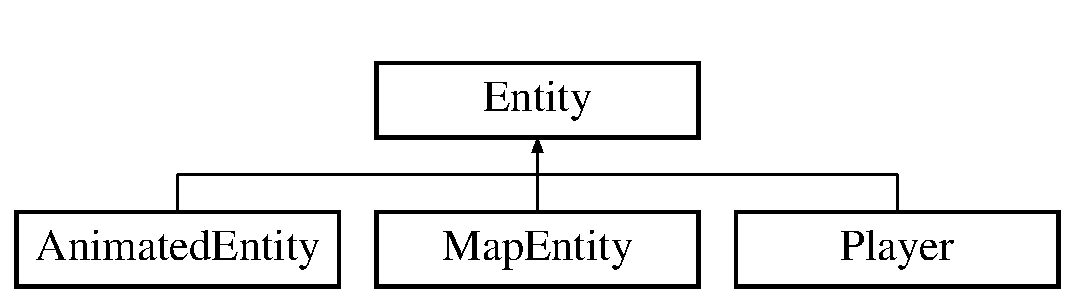
\includegraphics[height=2.000000cm]{class_entity}
\end{center}
\end{figure}
\subsection*{Public Member Functions}
\begin{DoxyCompactItemize}
\item 
\hyperlink{class_entity_a5c738f826217b3f8ce83d4c6b856e3ab}{Entity} (const sf\-::\-Texture \&texture, const sf\-::\-Vector2f \&pos, bool collidable=false)
\begin{DoxyCompactList}\small\item\em \hyperlink{class_entity}{Entity} ctor for making an entity. \end{DoxyCompactList}\item 
virtual \hyperlink{class_entity_adf6d3f7cb1b2ba029b6b048a395cc8ae}{$\sim$\-Entity} ()
\begin{DoxyCompactList}\small\item\em $\sim$\-Entity virtual call to destruct entities. \end{DoxyCompactList}\item 
virtual void \hyperlink{class_entity_a7e2a7c5df3bceaf41deea192eeba4d8f}{Update} ()
\begin{DoxyCompactList}\small\item\em Update virtual call to update entities, and their child class. \end{DoxyCompactList}\item 
virtual void \hyperlink{class_entity_ad8e60d2f123abe033b2653750e7944b3}{Draw} (sf\-::\-Render\-Window $\ast$p\-Window)
\begin{DoxyCompactList}\small\item\em Draw to a window. \end{DoxyCompactList}\item 
void \hyperlink{class_entity_a5009a2ec0e07f2decfdf80bce3a66d8e}{Set\-Is\-Collidable} (bool collidable)
\begin{DoxyCompactList}\small\item\em Set\-Is\-Collidable setter for the collidable flag. \end{DoxyCompactList}\item 
bool \hyperlink{class_entity_ac4cc6941a4a04be6e143ad240c499c46}{Get\-Is\-Collidable} () const 
\begin{DoxyCompactList}\small\item\em Get\-Is\-Collidable getter for the collidable flag. \end{DoxyCompactList}\item 
void \hyperlink{class_entity_abfdb5c682a32f0b5addfc77f171e4004}{Set\-Is\-Spawnable} (bool spawnable)
\begin{DoxyCompactList}\small\item\em Set\-Is\-Spawnable setter for the spawnable flag. \end{DoxyCompactList}\item 
bool \hyperlink{class_entity_aba3aa520f80f99a083fbfb2b604783cd}{Get\-Is\-Spawnable} () const 
\begin{DoxyCompactList}\small\item\em Get\-Is\-Spawnable getter for the spawnable flag. \end{DoxyCompactList}\item 
const sf\-::\-Vector2f \& \hyperlink{class_entity_a384e8c07dd367654bfba85c9921e0f88}{Get\-Position} ()
\begin{DoxyCompactList}\small\item\em Get\-Position getter for the position of the sprite, usually in top left corner. \end{DoxyCompactList}\item 
const sf\-::\-Float\-Rect \& \hyperlink{class_entity_a5e2cbcbaac883ed921888e6a90070d96}{Get\-Global\-Rect} ()
\begin{DoxyCompactList}\small\item\em Get\-Global\-Rect getter for the rectangle that borders the sprite. \end{DoxyCompactList}\item 
sf\-::\-Sprite $\ast$ \hyperlink{class_entity_a4481e6a0bf40afab75321078be213ebb}{Get\-Sprite} ()
\begin{DoxyCompactList}\small\item\em Get\-Sprite getter for the sf\-::\-Sprite this \hyperlink{class_entity}{Entity} represents. \end{DoxyCompactList}\end{DoxyCompactItemize}
\subsection*{Protected Attributes}
\begin{DoxyCompactItemize}
\item 
unique\-\_\-ptr$<$ sf\-::\-Sprite $>$ \hyperlink{class_entity_a52b9048640f6ffadfbc3e93d6184fe1f}{mp\-Sprite}
\item 
bool \hyperlink{class_entity_ade1f7c65bf9761c8e20188e67cb45556}{m\-Is\-Collidable}
\item 
bool \hyperlink{class_entity_a13cc8677fa51642cc3d60c13e9566dab}{m\-Is\-Spawnable}
\end{DoxyCompactItemize}


\subsection{Detailed Description}
The \hyperlink{class_entity}{Entity} class, represents a basic entity that exists in the 2d world. 

This class should be inherited from, to build complex types of objects that exist in the game world.

For example the player, enemies, pick up items, keys, doors, ect...

It can be drawable or non drawable. It can be a position that things may spawn on. 

Definition at line 30 of file Entity.\-hpp.



\subsection{Constructor \& Destructor Documentation}
\hypertarget{class_entity_a5c738f826217b3f8ce83d4c6b856e3ab}{\index{Entity@{Entity}!Entity@{Entity}}
\index{Entity@{Entity}!Entity@{Entity}}
\subsubsection[{Entity}]{\setlength{\rightskip}{0pt plus 5cm}Entity\-::\-Entity (
\begin{DoxyParamCaption}
\item[{const sf\-::\-Texture \&}]{texture, }
\item[{const sf\-::\-Vector2f \&}]{pos, }
\item[{bool}]{collidable = {\ttfamily false}}
\end{DoxyParamCaption}
)}}\label{class_entity_a5c738f826217b3f8ce83d4c6b856e3ab}


\hyperlink{class_entity}{Entity} ctor for making an entity. 


\begin{DoxyParams}{Parameters}
{\em texture} & The texture to use for this objects when drawing. \\
\hline
{\em pos} & The position, usually in top left corner. \\
\hline
{\em collidable} & Whether this object can be collided. \\
\hline
\end{DoxyParams}


Definition at line 11 of file Entity.\-cpp.

\hypertarget{class_entity_adf6d3f7cb1b2ba029b6b048a395cc8ae}{\index{Entity@{Entity}!$\sim$\-Entity@{$\sim$\-Entity}}
\index{$\sim$\-Entity@{$\sim$\-Entity}!Entity@{Entity}}
\subsubsection[{$\sim$\-Entity}]{\setlength{\rightskip}{0pt plus 5cm}Entity\-::$\sim$\-Entity (
\begin{DoxyParamCaption}
{}
\end{DoxyParamCaption}
)\hspace{0.3cm}{\ttfamily [virtual]}}}\label{class_entity_adf6d3f7cb1b2ba029b6b048a395cc8ae}


$\sim$\-Entity virtual call to destruct entities. 



Definition at line 20 of file Entity.\-cpp.



\subsection{Member Function Documentation}
\hypertarget{class_entity_ad8e60d2f123abe033b2653750e7944b3}{\index{Entity@{Entity}!Draw@{Draw}}
\index{Draw@{Draw}!Entity@{Entity}}
\subsubsection[{Draw}]{\setlength{\rightskip}{0pt plus 5cm}void Entity\-::\-Draw (
\begin{DoxyParamCaption}
\item[{sf\-::\-Render\-Window $\ast$}]{p\-Window}
\end{DoxyParamCaption}
)\hspace{0.3cm}{\ttfamily [virtual]}}}\label{class_entity_ad8e60d2f123abe033b2653750e7944b3}


Draw to a window. 


\begin{DoxyParams}{Parameters}
{\em p\-Window} & The window to draw to. \\
\hline
\end{DoxyParams}


Definition at line 30 of file Entity.\-cpp.

\hypertarget{class_entity_a5e2cbcbaac883ed921888e6a90070d96}{\index{Entity@{Entity}!Get\-Global\-Rect@{Get\-Global\-Rect}}
\index{Get\-Global\-Rect@{Get\-Global\-Rect}!Entity@{Entity}}
\subsubsection[{Get\-Global\-Rect}]{\setlength{\rightskip}{0pt plus 5cm}const sf\-::\-Float\-Rect \& Entity\-::\-Get\-Global\-Rect (
\begin{DoxyParamCaption}
{}
\end{DoxyParamCaption}
)}}\label{class_entity_a5e2cbcbaac883ed921888e6a90070d96}


Get\-Global\-Rect getter for the rectangle that borders the sprite. 

\begin{DoxyReturn}{Returns}
The rectangle of this object's sprite, in global coordinates. 
\end{DoxyReturn}


Definition at line 41 of file Entity.\-cpp.

\hypertarget{class_entity_ac4cc6941a4a04be6e143ad240c499c46}{\index{Entity@{Entity}!Get\-Is\-Collidable@{Get\-Is\-Collidable}}
\index{Get\-Is\-Collidable@{Get\-Is\-Collidable}!Entity@{Entity}}
\subsubsection[{Get\-Is\-Collidable}]{\setlength{\rightskip}{0pt plus 5cm}bool Entity\-::\-Get\-Is\-Collidable (
\begin{DoxyParamCaption}
{}
\end{DoxyParamCaption}
) const}}\label{class_entity_ac4cc6941a4a04be6e143ad240c499c46}


Get\-Is\-Collidable getter for the collidable flag. 

\begin{DoxyReturn}{Returns}
The current value for collidable. 
\end{DoxyReturn}


Definition at line 56 of file Entity.\-cpp.

\hypertarget{class_entity_aba3aa520f80f99a083fbfb2b604783cd}{\index{Entity@{Entity}!Get\-Is\-Spawnable@{Get\-Is\-Spawnable}}
\index{Get\-Is\-Spawnable@{Get\-Is\-Spawnable}!Entity@{Entity}}
\subsubsection[{Get\-Is\-Spawnable}]{\setlength{\rightskip}{0pt plus 5cm}bool Entity\-::\-Get\-Is\-Spawnable (
\begin{DoxyParamCaption}
{}
\end{DoxyParamCaption}
) const}}\label{class_entity_aba3aa520f80f99a083fbfb2b604783cd}


Get\-Is\-Spawnable getter for the spawnable flag. 

\begin{DoxyReturn}{Returns}
The current value for spawnable. 
\end{DoxyReturn}


Definition at line 66 of file Entity.\-cpp.

\hypertarget{class_entity_a384e8c07dd367654bfba85c9921e0f88}{\index{Entity@{Entity}!Get\-Position@{Get\-Position}}
\index{Get\-Position@{Get\-Position}!Entity@{Entity}}
\subsubsection[{Get\-Position}]{\setlength{\rightskip}{0pt plus 5cm}const sf\-::\-Vector2f \& Entity\-::\-Get\-Position (
\begin{DoxyParamCaption}
{}
\end{DoxyParamCaption}
)}}\label{class_entity_a384e8c07dd367654bfba85c9921e0f88}


Get\-Position getter for the position of the sprite, usually in top left corner. 

\begin{DoxyReturn}{Returns}
The current position. 
\end{DoxyReturn}


Definition at line 36 of file Entity.\-cpp.

\hypertarget{class_entity_a4481e6a0bf40afab75321078be213ebb}{\index{Entity@{Entity}!Get\-Sprite@{Get\-Sprite}}
\index{Get\-Sprite@{Get\-Sprite}!Entity@{Entity}}
\subsubsection[{Get\-Sprite}]{\setlength{\rightskip}{0pt plus 5cm}sf\-::\-Sprite $\ast$ Entity\-::\-Get\-Sprite (
\begin{DoxyParamCaption}
{}
\end{DoxyParamCaption}
)}}\label{class_entity_a4481e6a0bf40afab75321078be213ebb}


Get\-Sprite getter for the sf\-::\-Sprite this \hyperlink{class_entity}{Entity} represents. 

\begin{DoxyReturn}{Returns}
The sprite this \hyperlink{class_entity}{Entity} represents. 
\end{DoxyReturn}


Definition at line 46 of file Entity.\-cpp.

\hypertarget{class_entity_a5009a2ec0e07f2decfdf80bce3a66d8e}{\index{Entity@{Entity}!Set\-Is\-Collidable@{Set\-Is\-Collidable}}
\index{Set\-Is\-Collidable@{Set\-Is\-Collidable}!Entity@{Entity}}
\subsubsection[{Set\-Is\-Collidable}]{\setlength{\rightskip}{0pt plus 5cm}void Entity\-::\-Set\-Is\-Collidable (
\begin{DoxyParamCaption}
\item[{bool}]{collidable}
\end{DoxyParamCaption}
)}}\label{class_entity_a5009a2ec0e07f2decfdf80bce3a66d8e}


Set\-Is\-Collidable setter for the collidable flag. 


\begin{DoxyParams}{Parameters}
{\em collidable} & The value to set for collidable. \\
\hline
\end{DoxyParams}


Definition at line 51 of file Entity.\-cpp.

\hypertarget{class_entity_abfdb5c682a32f0b5addfc77f171e4004}{\index{Entity@{Entity}!Set\-Is\-Spawnable@{Set\-Is\-Spawnable}}
\index{Set\-Is\-Spawnable@{Set\-Is\-Spawnable}!Entity@{Entity}}
\subsubsection[{Set\-Is\-Spawnable}]{\setlength{\rightskip}{0pt plus 5cm}void Entity\-::\-Set\-Is\-Spawnable (
\begin{DoxyParamCaption}
\item[{bool}]{spawnable}
\end{DoxyParamCaption}
)}}\label{class_entity_abfdb5c682a32f0b5addfc77f171e4004}


Set\-Is\-Spawnable setter for the spawnable flag. 


\begin{DoxyParams}{Parameters}
{\em spawnable} & The value to set for spawnable. \\
\hline
\end{DoxyParams}


Definition at line 61 of file Entity.\-cpp.

\hypertarget{class_entity_a7e2a7c5df3bceaf41deea192eeba4d8f}{\index{Entity@{Entity}!Update@{Update}}
\index{Update@{Update}!Entity@{Entity}}
\subsubsection[{Update}]{\setlength{\rightskip}{0pt plus 5cm}void Entity\-::\-Update (
\begin{DoxyParamCaption}
{}
\end{DoxyParamCaption}
)\hspace{0.3cm}{\ttfamily [virtual]}}}\label{class_entity_a7e2a7c5df3bceaf41deea192eeba4d8f}


Update virtual call to update entities, and their child class. 



Reimplemented in \hyperlink{class_player_a05b60cac1922c5be5c1be16baffa4497}{Player}, and \hyperlink{class_animated_entity_af12d83ab3604a110e37c66c33206104b}{Animated\-Entity}.



Definition at line 25 of file Entity.\-cpp.



\subsection{Member Data Documentation}
\hypertarget{class_entity_ade1f7c65bf9761c8e20188e67cb45556}{\index{Entity@{Entity}!m\-Is\-Collidable@{m\-Is\-Collidable}}
\index{m\-Is\-Collidable@{m\-Is\-Collidable}!Entity@{Entity}}
\subsubsection[{m\-Is\-Collidable}]{\setlength{\rightskip}{0pt plus 5cm}bool Entity\-::m\-Is\-Collidable\hspace{0.3cm}{\ttfamily [protected]}}}\label{class_entity_ade1f7c65bf9761c8e20188e67cb45556}


Definition at line 101 of file Entity.\-hpp.

\hypertarget{class_entity_a13cc8677fa51642cc3d60c13e9566dab}{\index{Entity@{Entity}!m\-Is\-Spawnable@{m\-Is\-Spawnable}}
\index{m\-Is\-Spawnable@{m\-Is\-Spawnable}!Entity@{Entity}}
\subsubsection[{m\-Is\-Spawnable}]{\setlength{\rightskip}{0pt plus 5cm}bool Entity\-::m\-Is\-Spawnable\hspace{0.3cm}{\ttfamily [protected]}}}\label{class_entity_a13cc8677fa51642cc3d60c13e9566dab}


Definition at line 102 of file Entity.\-hpp.

\hypertarget{class_entity_a52b9048640f6ffadfbc3e93d6184fe1f}{\index{Entity@{Entity}!mp\-Sprite@{mp\-Sprite}}
\index{mp\-Sprite@{mp\-Sprite}!Entity@{Entity}}
\subsubsection[{mp\-Sprite}]{\setlength{\rightskip}{0pt plus 5cm}unique\-\_\-ptr$<$sf\-::\-Sprite$>$ Entity\-::mp\-Sprite\hspace{0.3cm}{\ttfamily [protected]}}}\label{class_entity_a52b9048640f6ffadfbc3e93d6184fe1f}


Definition at line 100 of file Entity.\-hpp.



The documentation for this class was generated from the following files\-:\begin{DoxyCompactItemize}
\item 
/home/chris/\-Projects/\-Sudden\-Awakening/\-Source/\hyperlink{_entity_8hpp}{Entity.\-hpp}\item 
/home/chris/\-Projects/\-Sudden\-Awakening/\-Source/\hyperlink{_entity_8cpp}{Entity.\-cpp}\end{DoxyCompactItemize}

\hypertarget{structtinyxml2_1_1_entity}{\section{tinyxml2\-:\-:Entity Struct Reference}
\label{structtinyxml2_1_1_entity}\index{tinyxml2\-::\-Entity@{tinyxml2\-::\-Entity}}
}
\subsection*{Public Attributes}
\begin{DoxyCompactItemize}
\item 
const char $\ast$ \hyperlink{structtinyxml2_1_1_entity_ab330f5d665d29bfc811ecfa76315894b}{pattern}
\item 
int \hyperlink{structtinyxml2_1_1_entity_a25e2b57cb59cb4fa68f283d7cb570f21}{length}
\item 
char \hyperlink{structtinyxml2_1_1_entity_a7334e81e33b4615655a403711b24f3ed}{value}
\end{DoxyCompactItemize}


\subsection{Detailed Description}


Definition at line 67 of file tinyxml2.\-cpp.



\subsection{Member Data Documentation}
\hypertarget{structtinyxml2_1_1_entity_a25e2b57cb59cb4fa68f283d7cb570f21}{\index{tinyxml2\-::\-Entity@{tinyxml2\-::\-Entity}!length@{length}}
\index{length@{length}!tinyxml2::Entity@{tinyxml2\-::\-Entity}}
\subsubsection[{length}]{\setlength{\rightskip}{0pt plus 5cm}int tinyxml2\-::\-Entity\-::length}}\label{structtinyxml2_1_1_entity_a25e2b57cb59cb4fa68f283d7cb570f21}


Definition at line 69 of file tinyxml2.\-cpp.

\hypertarget{structtinyxml2_1_1_entity_ab330f5d665d29bfc811ecfa76315894b}{\index{tinyxml2\-::\-Entity@{tinyxml2\-::\-Entity}!pattern@{pattern}}
\index{pattern@{pattern}!tinyxml2::Entity@{tinyxml2\-::\-Entity}}
\subsubsection[{pattern}]{\setlength{\rightskip}{0pt plus 5cm}const char$\ast$ tinyxml2\-::\-Entity\-::pattern}}\label{structtinyxml2_1_1_entity_ab330f5d665d29bfc811ecfa76315894b}


Definition at line 68 of file tinyxml2.\-cpp.

\hypertarget{structtinyxml2_1_1_entity_a7334e81e33b4615655a403711b24f3ed}{\index{tinyxml2\-::\-Entity@{tinyxml2\-::\-Entity}!value@{value}}
\index{value@{value}!tinyxml2::Entity@{tinyxml2\-::\-Entity}}
\subsubsection[{value}]{\setlength{\rightskip}{0pt plus 5cm}char tinyxml2\-::\-Entity\-::value}}\label{structtinyxml2_1_1_entity_a7334e81e33b4615655a403711b24f3ed}


Definition at line 70 of file tinyxml2.\-cpp.



The documentation for this struct was generated from the following file\-:\begin{DoxyCompactItemize}
\item 
/home/lee/\-Projects/\-Sudden\-Awakening/\-Source/\hyperlink{tinyxml2_8cpp}{tinyxml2.\-cpp}\end{DoxyCompactItemize}

\hypertarget{class_game}{\section{Game Class Reference}
\label{class_game}\index{Game@{Game}}
}


The \hyperlink{class_game}{Game} class everything for this game starts here.  




{\ttfamily \#include $<$Game.\-hpp$>$}

\subsection*{Public Member Functions}
\begin{DoxyCompactItemize}
\item 
\hyperlink{class_game_ad59df6562a58a614fda24622d3715b65}{Game} ()
\begin{DoxyCompactList}\small\item\em \hyperlink{class_game}{Game} only sets default values and tracks the singleton. \end{DoxyCompactList}\item 
\hyperlink{class_game_ae3d112ca6e0e55150d2fdbc704474530}{$\sim$\-Game} ()
\begin{DoxyCompactList}\small\item\em $\sim$\-Game dtor. \end{DoxyCompactList}\item 
bool \hyperlink{class_game_ab19596de871e7ce3ce5effc888c2a30b}{Init} ()
\begin{DoxyCompactList}\small\item\em Init all game/engine initialization starts here. \end{DoxyCompactList}\item 
int \hyperlink{class_game_a1880d9816a978b82bb91e4679743173d}{Run} ()
\begin{DoxyCompactList}\small\item\em Run is where all the game loop code is location and starts. \end{DoxyCompactList}\item 
void \hyperlink{class_game_a3b857f0272cf7d87010b8d95cd303e61}{Set\-New\-State\-Enum} (\hyperlink{_state_8hpp_a905494cc15ee9757a813dbfe4b1072fe}{State\-I\-D} state\-I\-D)
\begin{DoxyCompactList}\small\item\em Set\-New\-State\-Enum is the setter for the enum to tell the \hyperlink{class_game}{Game} to switch states on the next frame. \end{DoxyCompactList}\item 
sf\-::\-Render\-Window $\ast$ \hyperlink{class_game_a14241d779a3aa1dd9f4bb68cd018bbe8}{Get\-Window} ()
\begin{DoxyCompactList}\small\item\em Get\-Window getter for the render window. \end{DoxyCompactList}\item 
const sf\-::\-Font \& \hyperlink{class_game_ac508be317e5c3a7d7c41df0f9c740a96}{Get\-Button\-Font} () const 
\begin{DoxyCompactList}\small\item\em Get\-Button\-Font getter for the font to be used with the buttons. \end{DoxyCompactList}\item 
sf\-::\-Music $\ast$ \hyperlink{class_game_a156aeef24e86a468033121036fed239c}{Get\-Music} () const 
\begin{DoxyCompactList}\small\item\em Get\-Music. \end{DoxyCompactList}\item 
const \hyperlink{class_state}{State} $\ast$ \hyperlink{class_game_affa409c844370f25a5419a1f5225b0b5}{Get\-State} () const 
\item 
int \hyperlink{class_game_aa5913044e335b5624f52d6c95deed081}{Get\-Map\-Tile\-Size} () const 
\item 
double \hyperlink{class_game_a1a3becd8fb845889b4a2a86a32397393}{Get\-Frame\-Stamp\-D} () const 
\item 
double \hyperlink{class_game_a85bcfed7671cd09b10f3ea3c1c7a52db}{Get\-Frame\-Delta\-D} () const 
\item 
\hyperlink{_game_8hpp_a332b72dfb4bc8b4c16b8dc43864fe343}{Time\-Int} \hyperlink{class_game_aa7cf915c5e5f3a4b57b28eba915cfe2c}{Get\-Frame\-Stamp\-Int} () const 
\item 
\hyperlink{_game_8hpp_a332b72dfb4bc8b4c16b8dc43864fe343}{Time\-Int} \hyperlink{class_game_a60b3e0977db00a1c6c6ead044c7b1f27}{Get\-Frame\-Delta\-Int} () const 
\item 
const string \& \hyperlink{class_game_ad4eddde638de70fbbcdc212375fd7342}{Get\-Title\-Str} () const 
\end{DoxyCompactItemize}
\subsection*{Static Public Member Functions}
\begin{DoxyCompactItemize}
\item 
static \hyperlink{class_game}{Game} $\ast$ \hyperlink{class_game_a700c0cde9d2a8c5ad2672a8fdc0cfb4a}{Get} ()
\begin{DoxyCompactList}\small\item\em Get is the singleton getter. \end{DoxyCompactList}\end{DoxyCompactItemize}


\subsection{Detailed Description}
The \hyperlink{class_game}{Game} class everything for this game starts here. 

This is the big class that everything should be within.

It tracks time progression fps.

This class is responsible for making the window, creating the music functionality and some fonts ( used by the Buttons ).

It also stores a \hyperlink{class_state}{State} pointer which is how we handle states.

The \hyperlink{class_state}{State} children are the real states.

This class manages a singleton, you can access it through \hyperlink{class_game_a700c0cde9d2a8c5ad2672a8fdc0cfb4a}{Game\-::\-Get()} 

Definition at line 52 of file Game.\-hpp.



\subsection{Constructor \& Destructor Documentation}
\hypertarget{class_game_ad59df6562a58a614fda24622d3715b65}{\index{Game@{Game}!Game@{Game}}
\index{Game@{Game}!Game@{Game}}
\subsubsection[{Game}]{\setlength{\rightskip}{0pt plus 5cm}Game\-::\-Game (
\begin{DoxyParamCaption}
{}
\end{DoxyParamCaption}
)}}\label{class_game_ad59df6562a58a614fda24622d3715b65}


\hyperlink{class_game}{Game} only sets default values and tracks the singleton. 



Definition at line 28 of file Game.\-cpp.

\hypertarget{class_game_ae3d112ca6e0e55150d2fdbc704474530}{\index{Game@{Game}!$\sim$\-Game@{$\sim$\-Game}}
\index{$\sim$\-Game@{$\sim$\-Game}!Game@{Game}}
\subsubsection[{$\sim$\-Game}]{\setlength{\rightskip}{0pt plus 5cm}Game\-::$\sim$\-Game (
\begin{DoxyParamCaption}
{}
\end{DoxyParamCaption}
)}}\label{class_game_ae3d112ca6e0e55150d2fdbc704474530}


$\sim$\-Game dtor. 



Definition at line 48 of file Game.\-cpp.



\subsection{Member Function Documentation}
\hypertarget{class_game_a700c0cde9d2a8c5ad2672a8fdc0cfb4a}{\index{Game@{Game}!Get@{Get}}
\index{Get@{Get}!Game@{Game}}
\subsubsection[{Get}]{\setlength{\rightskip}{0pt plus 5cm}{\bf Game} $\ast$ Game\-::\-Get (
\begin{DoxyParamCaption}
{}
\end{DoxyParamCaption}
)\hspace{0.3cm}{\ttfamily [static]}}}\label{class_game_a700c0cde9d2a8c5ad2672a8fdc0cfb4a}


Get is the singleton getter. 

\begin{DoxyReturn}{Returns}
Pointer to the \hyperlink{class_game}{Game} singleton. 
\end{DoxyReturn}


Definition at line 53 of file Game.\-cpp.

\hypertarget{class_game_ac508be317e5c3a7d7c41df0f9c740a96}{\index{Game@{Game}!Get\-Button\-Font@{Get\-Button\-Font}}
\index{Get\-Button\-Font@{Get\-Button\-Font}!Game@{Game}}
\subsubsection[{Get\-Button\-Font}]{\setlength{\rightskip}{0pt plus 5cm}const sf\-::\-Font \& Game\-::\-Get\-Button\-Font (
\begin{DoxyParamCaption}
{}
\end{DoxyParamCaption}
) const}}\label{class_game_ac508be317e5c3a7d7c41df0f9c740a96}


Get\-Button\-Font getter for the font to be used with the buttons. 

\begin{DoxyReturn}{Returns}
The font to use for buttons. 
\end{DoxyReturn}


Definition at line 170 of file Game.\-cpp.

\hypertarget{class_game_a85bcfed7671cd09b10f3ea3c1c7a52db}{\index{Game@{Game}!Get\-Frame\-Delta\-D@{Get\-Frame\-Delta\-D}}
\index{Get\-Frame\-Delta\-D@{Get\-Frame\-Delta\-D}!Game@{Game}}
\subsubsection[{Get\-Frame\-Delta\-D}]{\setlength{\rightskip}{0pt plus 5cm}double Game\-::\-Get\-Frame\-Delta\-D (
\begin{DoxyParamCaption}
{}
\end{DoxyParamCaption}
) const}}\label{class_game_a85bcfed7671cd09b10f3ea3c1c7a52db}


Definition at line 202 of file Game.\-cpp.

\hypertarget{class_game_a60b3e0977db00a1c6c6ead044c7b1f27}{\index{Game@{Game}!Get\-Frame\-Delta\-Int@{Get\-Frame\-Delta\-Int}}
\index{Get\-Frame\-Delta\-Int@{Get\-Frame\-Delta\-Int}!Game@{Game}}
\subsubsection[{Get\-Frame\-Delta\-Int}]{\setlength{\rightskip}{0pt plus 5cm}{\bf Time\-Int} Game\-::\-Get\-Frame\-Delta\-Int (
\begin{DoxyParamCaption}
{}
\end{DoxyParamCaption}
) const}}\label{class_game_a60b3e0977db00a1c6c6ead044c7b1f27}


Definition at line 212 of file Game.\-cpp.

\hypertarget{class_game_a1a3becd8fb845889b4a2a86a32397393}{\index{Game@{Game}!Get\-Frame\-Stamp\-D@{Get\-Frame\-Stamp\-D}}
\index{Get\-Frame\-Stamp\-D@{Get\-Frame\-Stamp\-D}!Game@{Game}}
\subsubsection[{Get\-Frame\-Stamp\-D}]{\setlength{\rightskip}{0pt plus 5cm}double Game\-::\-Get\-Frame\-Stamp\-D (
\begin{DoxyParamCaption}
{}
\end{DoxyParamCaption}
) const}}\label{class_game_a1a3becd8fb845889b4a2a86a32397393}


Definition at line 197 of file Game.\-cpp.

\hypertarget{class_game_aa7cf915c5e5f3a4b57b28eba915cfe2c}{\index{Game@{Game}!Get\-Frame\-Stamp\-Int@{Get\-Frame\-Stamp\-Int}}
\index{Get\-Frame\-Stamp\-Int@{Get\-Frame\-Stamp\-Int}!Game@{Game}}
\subsubsection[{Get\-Frame\-Stamp\-Int}]{\setlength{\rightskip}{0pt plus 5cm}{\bf Time\-Int} Game\-::\-Get\-Frame\-Stamp\-Int (
\begin{DoxyParamCaption}
{}
\end{DoxyParamCaption}
) const}}\label{class_game_aa7cf915c5e5f3a4b57b28eba915cfe2c}


Definition at line 207 of file Game.\-cpp.

\hypertarget{class_game_aa5913044e335b5624f52d6c95deed081}{\index{Game@{Game}!Get\-Map\-Tile\-Size@{Get\-Map\-Tile\-Size}}
\index{Get\-Map\-Tile\-Size@{Get\-Map\-Tile\-Size}!Game@{Game}}
\subsubsection[{Get\-Map\-Tile\-Size}]{\setlength{\rightskip}{0pt plus 5cm}int Game\-::\-Get\-Map\-Tile\-Size (
\begin{DoxyParamCaption}
{}
\end{DoxyParamCaption}
) const}}\label{class_game_aa5913044e335b5624f52d6c95deed081}


Definition at line 192 of file Game.\-cpp.

\hypertarget{class_game_a156aeef24e86a468033121036fed239c}{\index{Game@{Game}!Get\-Music@{Get\-Music}}
\index{Get\-Music@{Get\-Music}!Game@{Game}}
\subsubsection[{Get\-Music}]{\setlength{\rightskip}{0pt plus 5cm}sf\-::\-Music $\ast$ Game\-::\-Get\-Music (
\begin{DoxyParamCaption}
{}
\end{DoxyParamCaption}
) const}}\label{class_game_a156aeef24e86a468033121036fed239c}


Get\-Music. 

\begin{DoxyReturn}{Returns}

\end{DoxyReturn}


Definition at line 175 of file Game.\-cpp.

\hypertarget{class_game_affa409c844370f25a5419a1f5225b0b5}{\index{Game@{Game}!Get\-State@{Get\-State}}
\index{Get\-State@{Get\-State}!Game@{Game}}
\subsubsection[{Get\-State}]{\setlength{\rightskip}{0pt plus 5cm}const {\bf State}$\ast$ Game\-::\-Get\-State (
\begin{DoxyParamCaption}
{}
\end{DoxyParamCaption}
) const}}\label{class_game_affa409c844370f25a5419a1f5225b0b5}
\hypertarget{class_game_ad4eddde638de70fbbcdc212375fd7342}{\index{Game@{Game}!Get\-Title\-Str@{Get\-Title\-Str}}
\index{Get\-Title\-Str@{Get\-Title\-Str}!Game@{Game}}
\subsubsection[{Get\-Title\-Str}]{\setlength{\rightskip}{0pt plus 5cm}const string \& Game\-::\-Get\-Title\-Str (
\begin{DoxyParamCaption}
{}
\end{DoxyParamCaption}
) const}}\label{class_game_ad4eddde638de70fbbcdc212375fd7342}


Definition at line 217 of file Game.\-cpp.

\hypertarget{class_game_a14241d779a3aa1dd9f4bb68cd018bbe8}{\index{Game@{Game}!Get\-Window@{Get\-Window}}
\index{Get\-Window@{Get\-Window}!Game@{Game}}
\subsubsection[{Get\-Window}]{\setlength{\rightskip}{0pt plus 5cm}sf\-::\-Render\-Window $\ast$ Game\-::\-Get\-Window (
\begin{DoxyParamCaption}
{}
\end{DoxyParamCaption}
)}}\label{class_game_a14241d779a3aa1dd9f4bb68cd018bbe8}


Get\-Window getter for the render window. 

\begin{DoxyReturn}{Returns}
Pointer to the render window for the game. 
\end{DoxyReturn}


Definition at line 165 of file Game.\-cpp.

\hypertarget{class_game_ab19596de871e7ce3ce5effc888c2a30b}{\index{Game@{Game}!Init@{Init}}
\index{Init@{Init}!Game@{Game}}
\subsubsection[{Init}]{\setlength{\rightskip}{0pt plus 5cm}bool Game\-::\-Init (
\begin{DoxyParamCaption}
{}
\end{DoxyParamCaption}
)}}\label{class_game_ab19596de871e7ce3ce5effc888c2a30b}


Init all game/engine initialization starts here. 

\begin{DoxyReturn}{Returns}
Success or fail of initialization of the entire game. 
\end{DoxyReturn}


Definition at line 58 of file Game.\-cpp.

\hypertarget{class_game_a1880d9816a978b82bb91e4679743173d}{\index{Game@{Game}!Run@{Run}}
\index{Run@{Run}!Game@{Game}}
\subsubsection[{Run}]{\setlength{\rightskip}{0pt plus 5cm}int Game\-::\-Run (
\begin{DoxyParamCaption}
{}
\end{DoxyParamCaption}
)}}\label{class_game_a1880d9816a978b82bb91e4679743173d}


Run is where all the game loop code is location and starts. 

\begin{DoxyReturn}{Returns}
The value that should be returned to the operating system to denote success or failure. 
\end{DoxyReturn}


Definition at line 101 of file Game.\-cpp.

\hypertarget{class_game_a3b857f0272cf7d87010b8d95cd303e61}{\index{Game@{Game}!Set\-New\-State\-Enum@{Set\-New\-State\-Enum}}
\index{Set\-New\-State\-Enum@{Set\-New\-State\-Enum}!Game@{Game}}
\subsubsection[{Set\-New\-State\-Enum}]{\setlength{\rightskip}{0pt plus 5cm}void Game\-::\-Set\-New\-State\-Enum (
\begin{DoxyParamCaption}
\item[{{\bf State\-I\-D}}]{state\-I\-D}
\end{DoxyParamCaption}
)}}\label{class_game_a3b857f0272cf7d87010b8d95cd303e61}


Set\-New\-State\-Enum is the setter for the enum to tell the \hyperlink{class_game}{Game} to switch states on the next frame. 


\begin{DoxyParams}{Parameters}
{\em state\-I\-D} & The value which represents a new state to change to. \\
\hline
\end{DoxyParams}


Definition at line 138 of file Game.\-cpp.



The documentation for this class was generated from the following files\-:\begin{DoxyCompactItemize}
\item 
Source/\hyperlink{_game_8hpp}{Game.\-hpp}\item 
Source/\hyperlink{_game_8cpp}{Game.\-cpp}\end{DoxyCompactItemize}

\hypertarget{class_level}{\section{Level Class Reference}
\label{class_level}\index{Level@{Level}}
}


{\ttfamily \#include $<$Level.\-hpp$>$}

Inheritance diagram for Level\-:\begin{figure}[H]
\begin{center}
\leavevmode
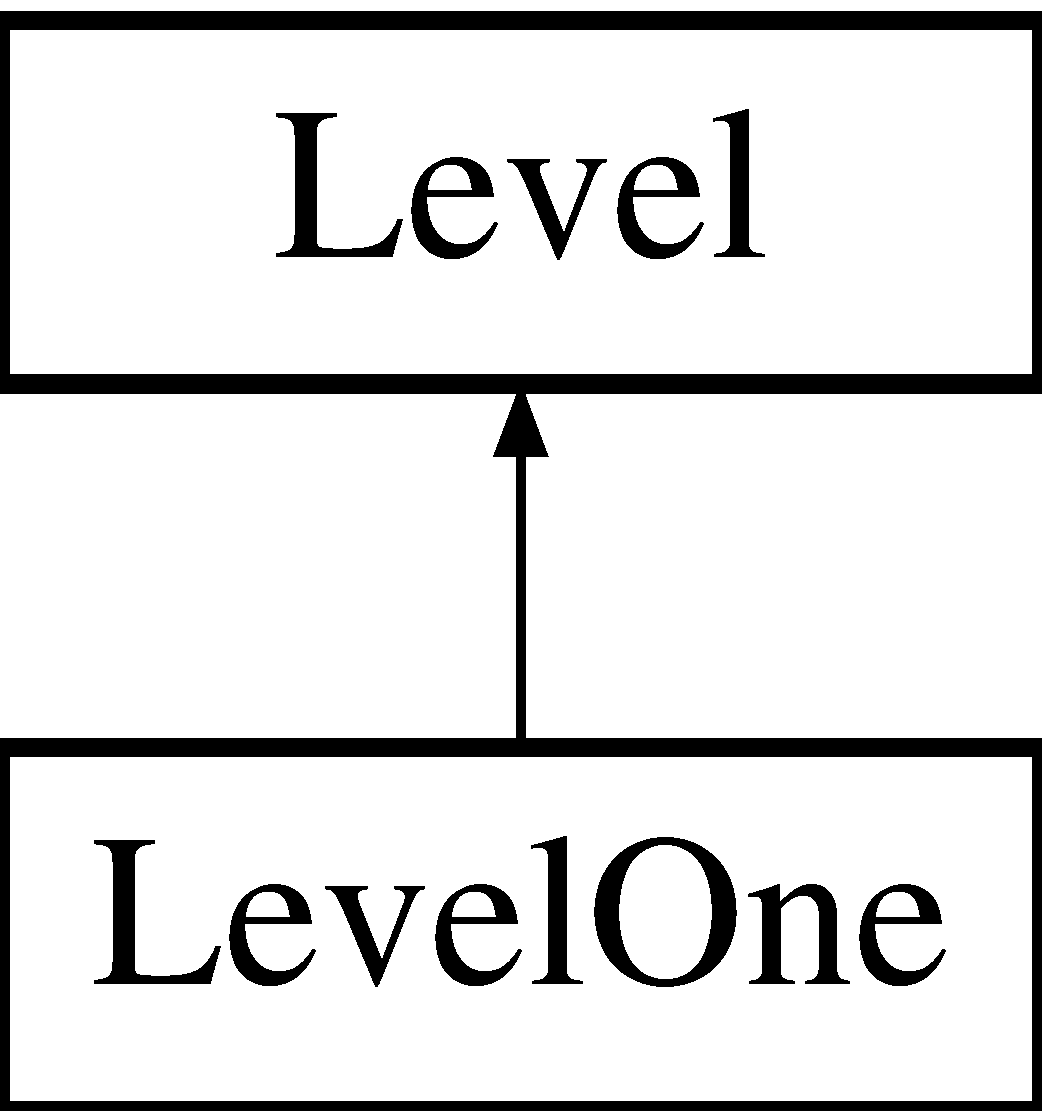
\includegraphics[height=2.000000cm]{class_level}
\end{center}
\end{figure}
\subsection*{Public Member Functions}
\begin{DoxyCompactItemize}
\item 
\hyperlink{class_level_a638468d7d98ba422bbcaf2e5ea05d421}{Level} (\hyperlink{_level_8hpp_aa0e387304096fe83aba77c85cb7be77a}{Level\-I\-D} level\-I\-D)
\item 
virtual \hyperlink{class_level_a249eac1e8f19ff44134efa5e986feaca}{$\sim$\-Level} ()
\item 
\hyperlink{_level_8hpp_aa0e387304096fe83aba77c85cb7be77a}{Level\-I\-D} \hyperlink{class_level_a03ef47d6709e8b62568cfaad9decfd0e}{Get\-I\-D} () const 
\item 
virtual void \hyperlink{class_level_a540d45e6d0ed7ce481d985881e8e27e2}{Update} ()=0
\item 
virtual void \hyperlink{class_level_a308eb5521217a781d2357ba83d041054}{Draw} ()=0
\item 
virtual void \hyperlink{class_level_a95bbafd05f5aa2396c36ff8343c62a2f}{Update\-Player} ()
\item 
virtual void \hyperlink{class_level_a26a3990bd47120e8e5c59f71d29ccb0a}{Load\-From\-X\-M\-L} (const string \&file)=0
\item 
virtual void \hyperlink{class_level_af8c86b5de9abc37b7f639fd9f5e9ea8e}{Process\-Event} (const sf\-::\-Event \&event)=0
\end{DoxyCompactItemize}
\subsection*{Protected Attributes}
\begin{DoxyCompactItemize}
\item 
\hyperlink{class_game}{Game} $\ast$ \hyperlink{class_level_a21c456b270db451d1da365d37e365b32}{mp\-Game}
\item 
\hyperlink{class_resource_manager}{Resource\-Manager}$<$ sf\-::\-Texture $>$ \hyperlink{class_level_a17bf54432fa53317ab5d7ffffbfdec6f}{m\-Textures}
\item 
unique\-\_\-ptr$<$ \hyperlink{class_audio_effects}{Audio\-Effects} $>$ \hyperlink{class_level_ad7ed6a1f41d6557b9ca3f7e62d705eb2}{mp\-Audio\-Effects}
\item 
unique\-\_\-ptr$<$ \hyperlink{class_tile_map}{Tile\-Map} $>$ \hyperlink{class_level_a2294842a4de2c0fbe9b28a670088b5c4}{mp\-Tile\-Map}
\item 
unique\-\_\-ptr$<$ \hyperlink{class_player}{Player} $>$ \hyperlink{class_level_a1cb20848f0e9d49a6469b4682e105d94}{mp\-Player}
\end{DoxyCompactItemize}
\subsection*{Friends}
\begin{DoxyCompactItemize}
\item 
void \hyperlink{class_level_ac44de73f21a1e6e5ae31d28a411395da}{Load\-Map\-Tiles\-From\-X\-M\-L} (\hyperlink{class_level}{Level} $\ast$, \hyperlink{classtinyxml2_1_1_x_m_l_element}{tinyxml2\-::\-X\-M\-L\-Element} $\ast$)
\end{DoxyCompactItemize}


\subsection{Detailed Description}


Definition at line 40 of file Level.\-hpp.



\subsection{Constructor \& Destructor Documentation}
\hypertarget{class_level_a638468d7d98ba422bbcaf2e5ea05d421}{\index{Level@{Level}!Level@{Level}}
\index{Level@{Level}!Level@{Level}}
\subsubsection[{Level}]{\setlength{\rightskip}{0pt plus 5cm}Level\-::\-Level (
\begin{DoxyParamCaption}
\item[{{\bf Level\-I\-D}}]{level\-I\-D}
\end{DoxyParamCaption}
)}}\label{class_level_a638468d7d98ba422bbcaf2e5ea05d421}


Definition at line 11 of file Level.\-cpp.

\hypertarget{class_level_a249eac1e8f19ff44134efa5e986feaca}{\index{Level@{Level}!$\sim$\-Level@{$\sim$\-Level}}
\index{$\sim$\-Level@{$\sim$\-Level}!Level@{Level}}
\subsubsection[{$\sim$\-Level}]{\setlength{\rightskip}{0pt plus 5cm}Level\-::$\sim$\-Level (
\begin{DoxyParamCaption}
{}
\end{DoxyParamCaption}
)\hspace{0.3cm}{\ttfamily [virtual]}}}\label{class_level_a249eac1e8f19ff44134efa5e986feaca}


Definition at line 22 of file Level.\-cpp.



\subsection{Member Function Documentation}
\hypertarget{class_level_a308eb5521217a781d2357ba83d041054}{\index{Level@{Level}!Draw@{Draw}}
\index{Draw@{Draw}!Level@{Level}}
\subsubsection[{Draw}]{\setlength{\rightskip}{0pt plus 5cm}virtual void Level\-::\-Draw (
\begin{DoxyParamCaption}
{}
\end{DoxyParamCaption}
)\hspace{0.3cm}{\ttfamily [pure virtual]}}}\label{class_level_a308eb5521217a781d2357ba83d041054}


Implemented in \hyperlink{class_level_one_ac39dc2f3934694f3428737b97001ff41}{Level\-One}.

\hypertarget{class_level_a03ef47d6709e8b62568cfaad9decfd0e}{\index{Level@{Level}!Get\-I\-D@{Get\-I\-D}}
\index{Get\-I\-D@{Get\-I\-D}!Level@{Level}}
\subsubsection[{Get\-I\-D}]{\setlength{\rightskip}{0pt plus 5cm}{\bf Level\-I\-D} Level\-::\-Get\-I\-D (
\begin{DoxyParamCaption}
{}
\end{DoxyParamCaption}
) const}}\label{class_level_a03ef47d6709e8b62568cfaad9decfd0e}


Definition at line 27 of file Level.\-cpp.

\hypertarget{class_level_a26a3990bd47120e8e5c59f71d29ccb0a}{\index{Level@{Level}!Load\-From\-X\-M\-L@{Load\-From\-X\-M\-L}}
\index{Load\-From\-X\-M\-L@{Load\-From\-X\-M\-L}!Level@{Level}}
\subsubsection[{Load\-From\-X\-M\-L}]{\setlength{\rightskip}{0pt plus 5cm}virtual void Level\-::\-Load\-From\-X\-M\-L (
\begin{DoxyParamCaption}
\item[{const string \&}]{file}
\end{DoxyParamCaption}
)\hspace{0.3cm}{\ttfamily [pure virtual]}}}\label{class_level_a26a3990bd47120e8e5c59f71d29ccb0a}


Implemented in \hyperlink{class_level_one_a6ff4ce4a9eaeb94987f897e47de62856}{Level\-One}.

\hypertarget{class_level_af8c86b5de9abc37b7f639fd9f5e9ea8e}{\index{Level@{Level}!Process\-Event@{Process\-Event}}
\index{Process\-Event@{Process\-Event}!Level@{Level}}
\subsubsection[{Process\-Event}]{\setlength{\rightskip}{0pt plus 5cm}virtual void Level\-::\-Process\-Event (
\begin{DoxyParamCaption}
\item[{const sf\-::\-Event \&}]{event}
\end{DoxyParamCaption}
)\hspace{0.3cm}{\ttfamily [pure virtual]}}}\label{class_level_af8c86b5de9abc37b7f639fd9f5e9ea8e}


Implemented in \hyperlink{class_level_one_ab806ffec162c436857edd2539e8f3d4e}{Level\-One}.

\hypertarget{class_level_a540d45e6d0ed7ce481d985881e8e27e2}{\index{Level@{Level}!Update@{Update}}
\index{Update@{Update}!Level@{Level}}
\subsubsection[{Update}]{\setlength{\rightskip}{0pt plus 5cm}virtual void Level\-::\-Update (
\begin{DoxyParamCaption}
{}
\end{DoxyParamCaption}
)\hspace{0.3cm}{\ttfamily [pure virtual]}}}\label{class_level_a540d45e6d0ed7ce481d985881e8e27e2}


Implemented in \hyperlink{class_level_one_ad0078eaa35f035c1a6ec7bf0bbef2fba}{Level\-One}.

\hypertarget{class_level_a95bbafd05f5aa2396c36ff8343c62a2f}{\index{Level@{Level}!Update\-Player@{Update\-Player}}
\index{Update\-Player@{Update\-Player}!Level@{Level}}
\subsubsection[{Update\-Player}]{\setlength{\rightskip}{0pt plus 5cm}void Level\-::\-Update\-Player (
\begin{DoxyParamCaption}
{}
\end{DoxyParamCaption}
)\hspace{0.3cm}{\ttfamily [virtual]}}}\label{class_level_a95bbafd05f5aa2396c36ff8343c62a2f}


Definition at line 32 of file Level.\-cpp.



\subsection{Friends And Related Function Documentation}
\hypertarget{class_level_ac44de73f21a1e6e5ae31d28a411395da}{\index{Level@{Level}!Load\-Map\-Tiles\-From\-X\-M\-L@{Load\-Map\-Tiles\-From\-X\-M\-L}}
\index{Load\-Map\-Tiles\-From\-X\-M\-L@{Load\-Map\-Tiles\-From\-X\-M\-L}!Level@{Level}}
\subsubsection[{Load\-Map\-Tiles\-From\-X\-M\-L}]{\setlength{\rightskip}{0pt plus 5cm}void Load\-Map\-Tiles\-From\-X\-M\-L (
\begin{DoxyParamCaption}
\item[{{\bf Level} $\ast$}]{, }
\item[{{\bf tinyxml2\-::\-X\-M\-L\-Element} $\ast$}]{}
\end{DoxyParamCaption}
)\hspace{0.3cm}{\ttfamily [friend]}}}\label{class_level_ac44de73f21a1e6e5ae31d28a411395da}


\subsection{Member Data Documentation}
\hypertarget{class_level_ad7ed6a1f41d6557b9ca3f7e62d705eb2}{\index{Level@{Level}!mp\-Audio\-Effects@{mp\-Audio\-Effects}}
\index{mp\-Audio\-Effects@{mp\-Audio\-Effects}!Level@{Level}}
\subsubsection[{mp\-Audio\-Effects}]{\setlength{\rightskip}{0pt plus 5cm}unique\-\_\-ptr$<${\bf Audio\-Effects}$>$ Level\-::mp\-Audio\-Effects\hspace{0.3cm}{\ttfamily [protected]}}}\label{class_level_ad7ed6a1f41d6557b9ca3f7e62d705eb2}


Definition at line 64 of file Level.\-hpp.

\hypertarget{class_level_a21c456b270db451d1da365d37e365b32}{\index{Level@{Level}!mp\-Game@{mp\-Game}}
\index{mp\-Game@{mp\-Game}!Level@{Level}}
\subsubsection[{mp\-Game}]{\setlength{\rightskip}{0pt plus 5cm}{\bf Game}$\ast$ Level\-::mp\-Game\hspace{0.3cm}{\ttfamily [protected]}}}\label{class_level_a21c456b270db451d1da365d37e365b32}


Definition at line 61 of file Level.\-hpp.

\hypertarget{class_level_a1cb20848f0e9d49a6469b4682e105d94}{\index{Level@{Level}!mp\-Player@{mp\-Player}}
\index{mp\-Player@{mp\-Player}!Level@{Level}}
\subsubsection[{mp\-Player}]{\setlength{\rightskip}{0pt plus 5cm}unique\-\_\-ptr$<$ {\bf Player} $>$ Level\-::mp\-Player\hspace{0.3cm}{\ttfamily [protected]}}}\label{class_level_a1cb20848f0e9d49a6469b4682e105d94}


Definition at line 66 of file Level.\-hpp.

\hypertarget{class_level_a2294842a4de2c0fbe9b28a670088b5c4}{\index{Level@{Level}!mp\-Tile\-Map@{mp\-Tile\-Map}}
\index{mp\-Tile\-Map@{mp\-Tile\-Map}!Level@{Level}}
\subsubsection[{mp\-Tile\-Map}]{\setlength{\rightskip}{0pt plus 5cm}unique\-\_\-ptr$<$ {\bf Tile\-Map} $>$ Level\-::mp\-Tile\-Map\hspace{0.3cm}{\ttfamily [protected]}}}\label{class_level_a2294842a4de2c0fbe9b28a670088b5c4}


Definition at line 65 of file Level.\-hpp.

\hypertarget{class_level_a17bf54432fa53317ab5d7ffffbfdec6f}{\index{Level@{Level}!m\-Textures@{m\-Textures}}
\index{m\-Textures@{m\-Textures}!Level@{Level}}
\subsubsection[{m\-Textures}]{\setlength{\rightskip}{0pt plus 5cm}{\bf Resource\-Manager}$<$sf\-::\-Texture$>$ Level\-::m\-Textures\hspace{0.3cm}{\ttfamily [protected]}}}\label{class_level_a17bf54432fa53317ab5d7ffffbfdec6f}


Definition at line 63 of file Level.\-hpp.



The documentation for this class was generated from the following files\-:\begin{DoxyCompactItemize}
\item 
Source/\hyperlink{_level_8hpp}{Level.\-hpp}\item 
Source/\hyperlink{_level_8cpp}{Level.\-cpp}\end{DoxyCompactItemize}

\hypertarget{class_level_one}{\section{Level\-One Class Reference}
\label{class_level_one}\index{Level\-One@{Level\-One}}
}


{\ttfamily \#include $<$Level\-One.\-hpp$>$}

Inheritance diagram for Level\-One\-:\begin{figure}[H]
\begin{center}
\leavevmode
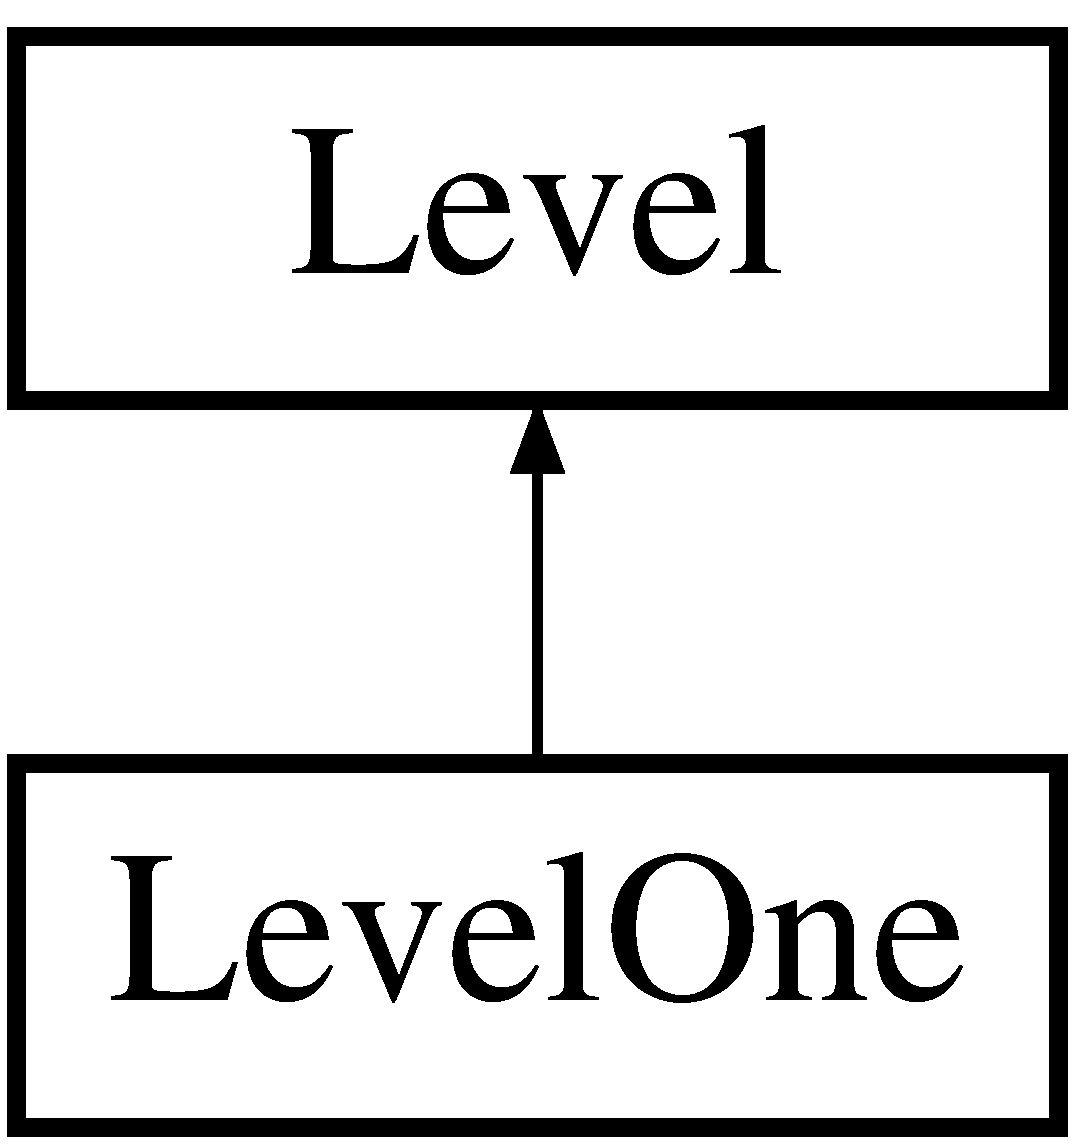
\includegraphics[height=2.000000cm]{class_level_one}
\end{center}
\end{figure}
\subsection*{Public Member Functions}
\begin{DoxyCompactItemize}
\item 
\hyperlink{class_level_one_a3fe4df62466654e6e7617377c8bd67a7}{Level\-One} ()
\item 
virtual \hyperlink{class_level_one_a43952923e3867bbdf882d18ac809ae34}{$\sim$\-Level\-One} ()
\item 
virtual void \hyperlink{class_level_one_ad0078eaa35f035c1a6ec7bf0bbef2fba}{Update} ()
\item 
virtual void \hyperlink{class_level_one_ac39dc2f3934694f3428737b97001ff41}{Draw} ()
\item 
virtual void \hyperlink{class_level_one_a6ff4ce4a9eaeb94987f897e47de62856}{Load\-From\-X\-M\-L} (const string \&file)
\item 
virtual void \hyperlink{class_level_one_ab806ffec162c436857edd2539e8f3d4e}{Process\-Event} (const sf\-::\-Event \&event)
\end{DoxyCompactItemize}
\subsection*{Additional Inherited Members}


\subsection{Detailed Description}


Definition at line 8 of file Level\-One.\-hpp.



\subsection{Constructor \& Destructor Documentation}
\hypertarget{class_level_one_a3fe4df62466654e6e7617377c8bd67a7}{\index{Level\-One@{Level\-One}!Level\-One@{Level\-One}}
\index{Level\-One@{Level\-One}!LevelOne@{Level\-One}}
\subsubsection[{Level\-One}]{\setlength{\rightskip}{0pt plus 5cm}Level\-One\-::\-Level\-One (
\begin{DoxyParamCaption}
{}
\end{DoxyParamCaption}
)}}\label{class_level_one_a3fe4df62466654e6e7617377c8bd67a7}


Definition at line 15 of file Level\-One.\-cpp.

\hypertarget{class_level_one_a43952923e3867bbdf882d18ac809ae34}{\index{Level\-One@{Level\-One}!$\sim$\-Level\-One@{$\sim$\-Level\-One}}
\index{$\sim$\-Level\-One@{$\sim$\-Level\-One}!LevelOne@{Level\-One}}
\subsubsection[{$\sim$\-Level\-One}]{\setlength{\rightskip}{0pt plus 5cm}Level\-One\-::$\sim$\-Level\-One (
\begin{DoxyParamCaption}
{}
\end{DoxyParamCaption}
)\hspace{0.3cm}{\ttfamily [virtual]}}}\label{class_level_one_a43952923e3867bbdf882d18ac809ae34}


Definition at line 23 of file Level\-One.\-cpp.



\subsection{Member Function Documentation}
\hypertarget{class_level_one_ac39dc2f3934694f3428737b97001ff41}{\index{Level\-One@{Level\-One}!Draw@{Draw}}
\index{Draw@{Draw}!LevelOne@{Level\-One}}
\subsubsection[{Draw}]{\setlength{\rightskip}{0pt plus 5cm}void Level\-One\-::\-Draw (
\begin{DoxyParamCaption}
{}
\end{DoxyParamCaption}
)\hspace{0.3cm}{\ttfamily [virtual]}}}\label{class_level_one_ac39dc2f3934694f3428737b97001ff41}


Implements \hyperlink{class_level_a308eb5521217a781d2357ba83d041054}{Level}.



Definition at line 34 of file Level\-One.\-cpp.

\hypertarget{class_level_one_a6ff4ce4a9eaeb94987f897e47de62856}{\index{Level\-One@{Level\-One}!Load\-From\-X\-M\-L@{Load\-From\-X\-M\-L}}
\index{Load\-From\-X\-M\-L@{Load\-From\-X\-M\-L}!LevelOne@{Level\-One}}
\subsubsection[{Load\-From\-X\-M\-L}]{\setlength{\rightskip}{0pt plus 5cm}void Level\-One\-::\-Load\-From\-X\-M\-L (
\begin{DoxyParamCaption}
\item[{const string \&}]{file}
\end{DoxyParamCaption}
)\hspace{0.3cm}{\ttfamily [virtual]}}}\label{class_level_one_a6ff4ce4a9eaeb94987f897e47de62856}


Implements \hyperlink{class_level_a26a3990bd47120e8e5c59f71d29ccb0a}{Level}.



Definition at line 45 of file Level\-One.\-cpp.

\hypertarget{class_level_one_ab806ffec162c436857edd2539e8f3d4e}{\index{Level\-One@{Level\-One}!Process\-Event@{Process\-Event}}
\index{Process\-Event@{Process\-Event}!LevelOne@{Level\-One}}
\subsubsection[{Process\-Event}]{\setlength{\rightskip}{0pt plus 5cm}void Level\-One\-::\-Process\-Event (
\begin{DoxyParamCaption}
\item[{const sf\-::\-Event \&}]{event}
\end{DoxyParamCaption}
)\hspace{0.3cm}{\ttfamily [virtual]}}}\label{class_level_one_ab806ffec162c436857edd2539e8f3d4e}


Implements \hyperlink{class_level_af8c86b5de9abc37b7f639fd9f5e9ea8e}{Level}.



Definition at line 88 of file Level\-One.\-cpp.

\hypertarget{class_level_one_ad0078eaa35f035c1a6ec7bf0bbef2fba}{\index{Level\-One@{Level\-One}!Update@{Update}}
\index{Update@{Update}!LevelOne@{Level\-One}}
\subsubsection[{Update}]{\setlength{\rightskip}{0pt plus 5cm}void Level\-One\-::\-Update (
\begin{DoxyParamCaption}
{}
\end{DoxyParamCaption}
)\hspace{0.3cm}{\ttfamily [virtual]}}}\label{class_level_one_ad0078eaa35f035c1a6ec7bf0bbef2fba}


Implements \hyperlink{class_level_a540d45e6d0ed7ce481d985881e8e27e2}{Level}.



Definition at line 28 of file Level\-One.\-cpp.



The documentation for this class was generated from the following files\-:\begin{DoxyCompactItemize}
\item 
Source/\hyperlink{_level_one_8hpp}{Level\-One.\-hpp}\item 
Source/\hyperlink{_level_one_8cpp}{Level\-One.\-cpp}\end{DoxyCompactItemize}

\hypertarget{class_logger}{\section{Logger Class Reference}
\label{class_logger}\index{Logger@{Logger}}
}


{\ttfamily \#include $<$Logger.\-hpp$>$}

\subsection*{Public Member Functions}
\begin{DoxyCompactItemize}
\item 
\hyperlink{class_logger_a0a05ff69f854770ba73be8da23087c6f}{Logger} (const std\-::string \&file)
\item 
\hyperlink{class_logger_acb668a9e186a25fbaad2e4af6d1ed00a}{$\sim$\-Logger} ()
\item 
void \hyperlink{class_logger_a869a3da0fbc98ea124c8142441ba9979}{Func\-Begin} (const string \&function=\char`\"{}Not supported\char`\"{})
\item 
void \hyperlink{class_logger_af6534aa3be0f75da9476bdf98b0cd6bf}{Func\-End\-Success} (const string \&function=\char`\"{}Not supported\char`\"{})
\item 
void \hyperlink{class_logger_a0c51ea7dd128afa466379dee45487377}{Message} (const string \&desc, const string \&file, const unsigned long long line)
\item 
void \hyperlink{class_logger_a61d131fd8e6096c8711e5b05efe15761}{Success} (const string \&desc, const string \&file, const unsigned long long line)
\item 
void \hyperlink{class_logger_afc4de5bbb2fb2b647f0dc86cafc037cf}{Warning} (const string \&desc, const string \&file, const unsigned long long line)
\item 
void \hyperlink{class_logger_a60d34309f66f5ce02675bbdaca545094}{Exception} (const std\-::exception \&except)
\item 
void \hyperlink{class_logger_a7e67b48e4e24f6f2fb03ff40bbeeb9ad}{Error} (const string \&file, const unsigned long long line, const string \&desc, const string \&error=string(), const int error\-Code=0)
\item 
void \hyperlink{class_logger_aa7909a3a0a254c2e90abc09911ba9a20}{Failure} (const string \&file, const unsigned long long line, const string \&desc)
\end{DoxyCompactItemize}
\subsection*{Protected Member Functions}
\begin{DoxyCompactItemize}
\item 
void \hyperlink{class_logger_a6360e51a7be091da6419667be9baaf4d}{Log\-File\-Line\-Desc} (const string \&file, const unsigned long long line, const string \&desc)
\item 
void \hyperlink{class_logger_aa93d938b1a593173396d677f34dfbb1c}{Put\-Time\-Str} ()
\end{DoxyCompactItemize}
\subsection*{Protected Attributes}
\begin{DoxyCompactItemize}
\item 
ofstream $\ast$ \hyperlink{class_logger_a69b68a1b1da1754873ebb48a9b045f74}{mp\-Ofs}
\end{DoxyCompactItemize}


\subsection{Detailed Description}


Definition at line 61 of file Logger.\-hpp.



\subsection{Constructor \& Destructor Documentation}
\hypertarget{class_logger_a0a05ff69f854770ba73be8da23087c6f}{\index{Logger@{Logger}!Logger@{Logger}}
\index{Logger@{Logger}!Logger@{Logger}}
\subsubsection[{Logger}]{\setlength{\rightskip}{0pt plus 5cm}Logger\-::\-Logger (
\begin{DoxyParamCaption}
\item[{const std\-::string \&}]{file}
\end{DoxyParamCaption}
)}}\label{class_logger_a0a05ff69f854770ba73be8da23087c6f}


Definition at line 49 of file Logger.\-cpp.

\hypertarget{class_logger_acb668a9e186a25fbaad2e4af6d1ed00a}{\index{Logger@{Logger}!$\sim$\-Logger@{$\sim$\-Logger}}
\index{$\sim$\-Logger@{$\sim$\-Logger}!Logger@{Logger}}
\subsubsection[{$\sim$\-Logger}]{\setlength{\rightskip}{0pt plus 5cm}Logger\-::$\sim$\-Logger (
\begin{DoxyParamCaption}
{}
\end{DoxyParamCaption}
)}}\label{class_logger_acb668a9e186a25fbaad2e4af6d1ed00a}


Definition at line 60 of file Logger.\-cpp.



\subsection{Member Function Documentation}
\hypertarget{class_logger_a7e67b48e4e24f6f2fb03ff40bbeeb9ad}{\index{Logger@{Logger}!Error@{Error}}
\index{Error@{Error}!Logger@{Logger}}
\subsubsection[{Error}]{\setlength{\rightskip}{0pt plus 5cm}void Logger\-::\-Error (
\begin{DoxyParamCaption}
\item[{const string \&}]{file, }
\item[{const unsigned long long}]{line, }
\item[{const string \&}]{desc, }
\item[{const string \&}]{error = {\ttfamily string()}, }
\item[{const int}]{error\-Code = {\ttfamily 0}}
\end{DoxyParamCaption}
)}}\label{class_logger_a7e67b48e4e24f6f2fb03ff40bbeeb9ad}


Definition at line 106 of file Logger.\-cpp.

\hypertarget{class_logger_a60d34309f66f5ce02675bbdaca545094}{\index{Logger@{Logger}!Exception@{Exception}}
\index{Exception@{Exception}!Logger@{Logger}}
\subsubsection[{Exception}]{\setlength{\rightskip}{0pt plus 5cm}void Logger\-::\-Exception (
\begin{DoxyParamCaption}
\item[{const std\-::exception \&}]{except}
\end{DoxyParamCaption}
)}}\label{class_logger_a60d34309f66f5ce02675bbdaca545094}


Definition at line 99 of file Logger.\-cpp.

\hypertarget{class_logger_aa7909a3a0a254c2e90abc09911ba9a20}{\index{Logger@{Logger}!Failure@{Failure}}
\index{Failure@{Failure}!Logger@{Logger}}
\subsubsection[{Failure}]{\setlength{\rightskip}{0pt plus 5cm}void Logger\-::\-Failure (
\begin{DoxyParamCaption}
\item[{const string \&}]{file, }
\item[{const unsigned long long}]{line, }
\item[{const string \&}]{desc}
\end{DoxyParamCaption}
)}}\label{class_logger_aa7909a3a0a254c2e90abc09911ba9a20}


Definition at line 119 of file Logger.\-cpp.

\hypertarget{class_logger_a869a3da0fbc98ea124c8142441ba9979}{\index{Logger@{Logger}!Func\-Begin@{Func\-Begin}}
\index{Func\-Begin@{Func\-Begin}!Logger@{Logger}}
\subsubsection[{Func\-Begin}]{\setlength{\rightskip}{0pt plus 5cm}void Logger\-::\-Func\-Begin (
\begin{DoxyParamCaption}
\item[{const string \&}]{function = {\ttfamily \char`\"{}Not~supported\char`\"{}}}
\end{DoxyParamCaption}
)}}\label{class_logger_a869a3da0fbc98ea124c8142441ba9979}


Definition at line 66 of file Logger.\-cpp.

\hypertarget{class_logger_af6534aa3be0f75da9476bdf98b0cd6bf}{\index{Logger@{Logger}!Func\-End\-Success@{Func\-End\-Success}}
\index{Func\-End\-Success@{Func\-End\-Success}!Logger@{Logger}}
\subsubsection[{Func\-End\-Success}]{\setlength{\rightskip}{0pt plus 5cm}void Logger\-::\-Func\-End\-Success (
\begin{DoxyParamCaption}
\item[{const string \&}]{function = {\ttfamily \char`\"{}Not~supported\char`\"{}}}
\end{DoxyParamCaption}
)}}\label{class_logger_af6534aa3be0f75da9476bdf98b0cd6bf}


Definition at line 72 of file Logger.\-cpp.

\hypertarget{class_logger_a6360e51a7be091da6419667be9baaf4d}{\index{Logger@{Logger}!Log\-File\-Line\-Desc@{Log\-File\-Line\-Desc}}
\index{Log\-File\-Line\-Desc@{Log\-File\-Line\-Desc}!Logger@{Logger}}
\subsubsection[{Log\-File\-Line\-Desc}]{\setlength{\rightskip}{0pt plus 5cm}void Logger\-::\-Log\-File\-Line\-Desc (
\begin{DoxyParamCaption}
\item[{const string \&}]{file, }
\item[{const unsigned long long}]{line, }
\item[{const string \&}]{desc}
\end{DoxyParamCaption}
)\hspace{0.3cm}{\ttfamily [protected]}}}\label{class_logger_a6360e51a7be091da6419667be9baaf4d}


Definition at line 138 of file Logger.\-cpp.

\hypertarget{class_logger_a0c51ea7dd128afa466379dee45487377}{\index{Logger@{Logger}!Message@{Message}}
\index{Message@{Message}!Logger@{Logger}}
\subsubsection[{Message}]{\setlength{\rightskip}{0pt plus 5cm}void Logger\-::\-Message (
\begin{DoxyParamCaption}
\item[{const string \&}]{desc, }
\item[{const string \&}]{file, }
\item[{const unsigned long long}]{line}
\end{DoxyParamCaption}
)}}\label{class_logger_a0c51ea7dd128afa466379dee45487377}


Definition at line 78 of file Logger.\-cpp.

\hypertarget{class_logger_aa93d938b1a593173396d677f34dfbb1c}{\index{Logger@{Logger}!Put\-Time\-Str@{Put\-Time\-Str}}
\index{Put\-Time\-Str@{Put\-Time\-Str}!Logger@{Logger}}
\subsubsection[{Put\-Time\-Str}]{\setlength{\rightskip}{0pt plus 5cm}void Logger\-::\-Put\-Time\-Str (
\begin{DoxyParamCaption}
{}
\end{DoxyParamCaption}
)\hspace{0.3cm}{\ttfamily [protected]}}}\label{class_logger_aa93d938b1a593173396d677f34dfbb1c}


Definition at line 126 of file Logger.\-cpp.

\hypertarget{class_logger_a61d131fd8e6096c8711e5b05efe15761}{\index{Logger@{Logger}!Success@{Success}}
\index{Success@{Success}!Logger@{Logger}}
\subsubsection[{Success}]{\setlength{\rightskip}{0pt plus 5cm}void Logger\-::\-Success (
\begin{DoxyParamCaption}
\item[{const string \&}]{desc, }
\item[{const string \&}]{file, }
\item[{const unsigned long long}]{line}
\end{DoxyParamCaption}
)}}\label{class_logger_a61d131fd8e6096c8711e5b05efe15761}


Definition at line 85 of file Logger.\-cpp.

\hypertarget{class_logger_afc4de5bbb2fb2b647f0dc86cafc037cf}{\index{Logger@{Logger}!Warning@{Warning}}
\index{Warning@{Warning}!Logger@{Logger}}
\subsubsection[{Warning}]{\setlength{\rightskip}{0pt plus 5cm}void Logger\-::\-Warning (
\begin{DoxyParamCaption}
\item[{const string \&}]{desc, }
\item[{const string \&}]{file, }
\item[{const unsigned long long}]{line}
\end{DoxyParamCaption}
)}}\label{class_logger_afc4de5bbb2fb2b647f0dc86cafc037cf}


Definition at line 92 of file Logger.\-cpp.



\subsection{Member Data Documentation}
\hypertarget{class_logger_a69b68a1b1da1754873ebb48a9b045f74}{\index{Logger@{Logger}!mp\-Ofs@{mp\-Ofs}}
\index{mp\-Ofs@{mp\-Ofs}!Logger@{Logger}}
\subsubsection[{mp\-Ofs}]{\setlength{\rightskip}{0pt plus 5cm}ofstream$\ast$ Logger\-::mp\-Ofs\hspace{0.3cm}{\ttfamily [protected]}}}\label{class_logger_a69b68a1b1da1754873ebb48a9b045f74}


Definition at line 90 of file Logger.\-hpp.



The documentation for this class was generated from the following files\-:\begin{DoxyCompactItemize}
\item 
/home/lee/\-Projects/\-Sudden\-Awakening/\-Source/\hyperlink{_logger_8hpp}{Logger.\-hpp}\item 
/home/lee/\-Projects/\-Sudden\-Awakening/\-Source/\hyperlink{_logger_8cpp}{Logger.\-cpp}\end{DoxyCompactItemize}

\hypertarget{class_map_entity}{\section{Map\-Entity Class Reference}
\label{class_map_entity}\index{Map\-Entity@{Map\-Entity}}
}


{\ttfamily \#include $<$Entity.\-hpp$>$}

Inheritance diagram for Map\-Entity\-:\begin{figure}[H]
\begin{center}
\leavevmode
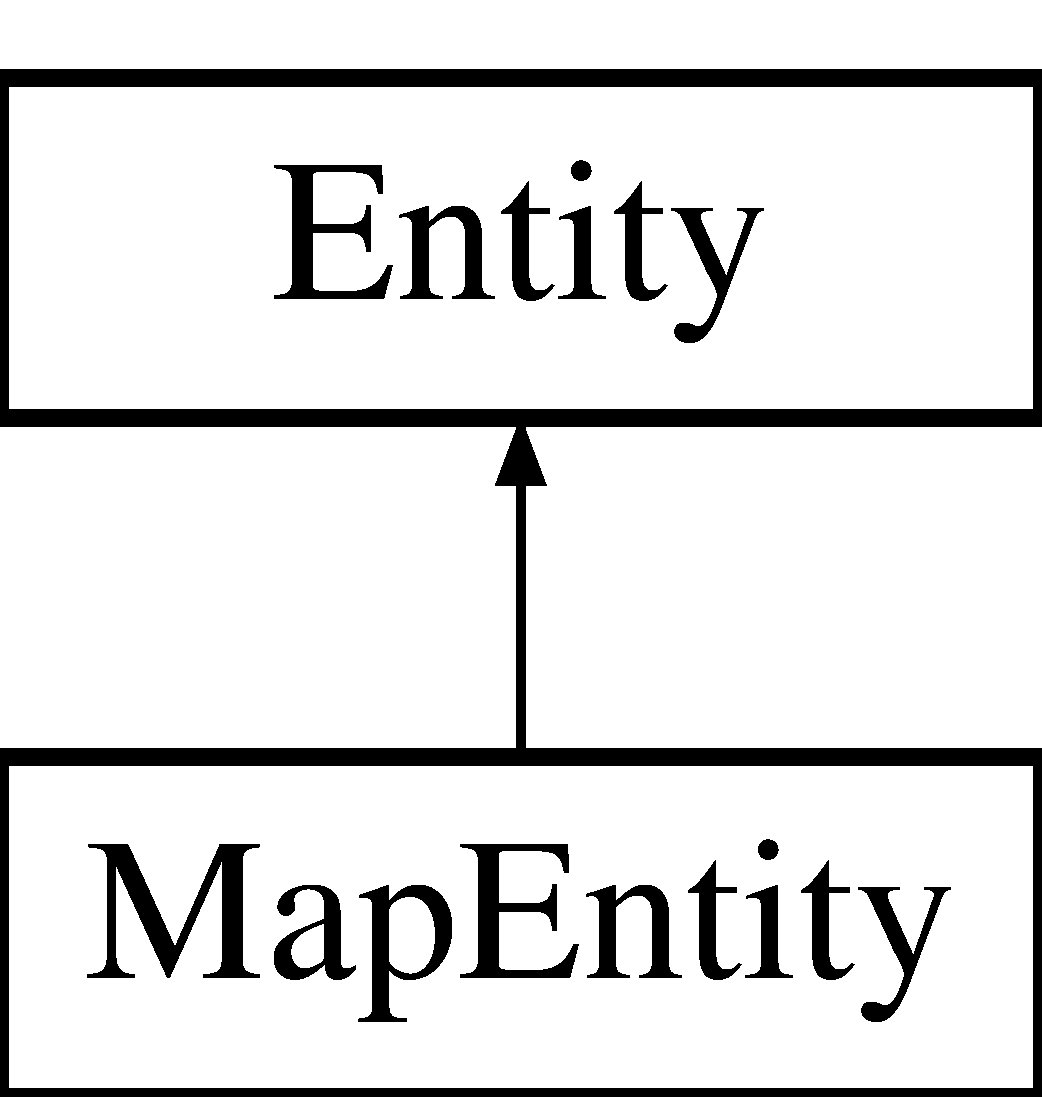
\includegraphics[height=2.000000cm]{class_map_entity}
\end{center}
\end{figure}
\subsection*{Public Member Functions}
\begin{DoxyCompactItemize}
\item 
\hyperlink{class_map_entity_a0cb75a3daea11151b3323d7646c91438}{Map\-Entity} (const sf\-::\-Texture \&texture, const sf\-::\-Int\-Rect \&tex\-Rect, const sf\-::\-Vector2f \&pos)
\item 
virtual \hyperlink{class_map_entity_adbd58311e0e21fa1e7a90709d25625df}{$\sim$\-Map\-Entity} ()
\end{DoxyCompactItemize}
\subsection*{Additional Inherited Members}


\subsection{Detailed Description}


Definition at line 238 of file Entity.\-hpp.



\subsection{Constructor \& Destructor Documentation}
\hypertarget{class_map_entity_a0cb75a3daea11151b3323d7646c91438}{\index{Map\-Entity@{Map\-Entity}!Map\-Entity@{Map\-Entity}}
\index{Map\-Entity@{Map\-Entity}!MapEntity@{Map\-Entity}}
\subsubsection[{Map\-Entity}]{\setlength{\rightskip}{0pt plus 5cm}Map\-Entity\-::\-Map\-Entity (
\begin{DoxyParamCaption}
\item[{const sf\-::\-Texture \&}]{texture, }
\item[{const sf\-::\-Int\-Rect \&}]{tex\-Rect, }
\item[{const sf\-::\-Vector2f \&}]{pos}
\end{DoxyParamCaption}
)}}\label{class_map_entity_a0cb75a3daea11151b3323d7646c91438}


Definition at line 195 of file Entity.\-cpp.

\hypertarget{class_map_entity_adbd58311e0e21fa1e7a90709d25625df}{\index{Map\-Entity@{Map\-Entity}!$\sim$\-Map\-Entity@{$\sim$\-Map\-Entity}}
\index{$\sim$\-Map\-Entity@{$\sim$\-Map\-Entity}!MapEntity@{Map\-Entity}}
\subsubsection[{$\sim$\-Map\-Entity}]{\setlength{\rightskip}{0pt plus 5cm}Map\-Entity\-::$\sim$\-Map\-Entity (
\begin{DoxyParamCaption}
{}
\end{DoxyParamCaption}
)\hspace{0.3cm}{\ttfamily [virtual]}}}\label{class_map_entity_adbd58311e0e21fa1e7a90709d25625df}


Definition at line 202 of file Entity.\-cpp.



The documentation for this class was generated from the following files\-:\begin{DoxyCompactItemize}
\item 
Source/\hyperlink{_entity_8hpp}{Entity.\-hpp}\item 
Source/\hyperlink{_entity_8cpp}{Entity.\-cpp}\end{DoxyCompactItemize}

\hypertarget{classtinyxml2_1_1_mem_pool}{\section{tinyxml2\-:\-:Mem\-Pool Class Reference}
\label{classtinyxml2_1_1_mem_pool}\index{tinyxml2\-::\-Mem\-Pool@{tinyxml2\-::\-Mem\-Pool}}
}


{\ttfamily \#include $<$tinyxml2.\-hpp$>$}

Inheritance diagram for tinyxml2\-:\-:Mem\-Pool\-:\begin{figure}[H]
\begin{center}
\leavevmode
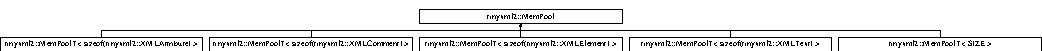
\includegraphics[height=0.691358cm]{classtinyxml2_1_1_mem_pool}
\end{center}
\end{figure}
\subsection*{Public Member Functions}
\begin{DoxyCompactItemize}
\item 
\hyperlink{classtinyxml2_1_1_mem_pool_a9101a0083d7370c85bd5aaaba7157f84}{Mem\-Pool} ()
\item 
virtual \hyperlink{classtinyxml2_1_1_mem_pool_ae55ad9e3faeca702e6ccbb38fdbcad72}{$\sim$\-Mem\-Pool} ()
\item 
virtual int \hyperlink{classtinyxml2_1_1_mem_pool_a0c518d49e3a94bde566f61e13b7240bb}{Item\-Size} () const =0
\item 
virtual void $\ast$ \hyperlink{classtinyxml2_1_1_mem_pool_a4f977b5fed752c0bbfe5295f469d6449}{Alloc} ()=0
\item 
virtual void \hyperlink{classtinyxml2_1_1_mem_pool_a49e3bfac2cba2ebd6776b31e571f64f7}{Free} (void $\ast$)=0
\item 
virtual void \hyperlink{classtinyxml2_1_1_mem_pool_ac5804dd1387b2e4de5eef710076a0db1}{Set\-Tracked} ()=0
\end{DoxyCompactItemize}


\subsection{Detailed Description}


Definition at line 295 of file tinyxml2.\-hpp.



\subsection{Constructor \& Destructor Documentation}
\hypertarget{classtinyxml2_1_1_mem_pool_a9101a0083d7370c85bd5aaaba7157f84}{\index{tinyxml2\-::\-Mem\-Pool@{tinyxml2\-::\-Mem\-Pool}!Mem\-Pool@{Mem\-Pool}}
\index{Mem\-Pool@{Mem\-Pool}!tinyxml2::MemPool@{tinyxml2\-::\-Mem\-Pool}}
\subsubsection[{Mem\-Pool}]{\setlength{\rightskip}{0pt plus 5cm}tinyxml2\-::\-Mem\-Pool\-::\-Mem\-Pool (
\begin{DoxyParamCaption}
{}
\end{DoxyParamCaption}
)\hspace{0.3cm}{\ttfamily [inline]}}}\label{classtinyxml2_1_1_mem_pool_a9101a0083d7370c85bd5aaaba7157f84}


Definition at line 298 of file tinyxml2.\-hpp.

\hypertarget{classtinyxml2_1_1_mem_pool_ae55ad9e3faeca702e6ccbb38fdbcad72}{\index{tinyxml2\-::\-Mem\-Pool@{tinyxml2\-::\-Mem\-Pool}!$\sim$\-Mem\-Pool@{$\sim$\-Mem\-Pool}}
\index{$\sim$\-Mem\-Pool@{$\sim$\-Mem\-Pool}!tinyxml2::MemPool@{tinyxml2\-::\-Mem\-Pool}}
\subsubsection[{$\sim$\-Mem\-Pool}]{\setlength{\rightskip}{0pt plus 5cm}virtual tinyxml2\-::\-Mem\-Pool\-::$\sim$\-Mem\-Pool (
\begin{DoxyParamCaption}
{}
\end{DoxyParamCaption}
)\hspace{0.3cm}{\ttfamily [inline]}, {\ttfamily [virtual]}}}\label{classtinyxml2_1_1_mem_pool_ae55ad9e3faeca702e6ccbb38fdbcad72}


Definition at line 299 of file tinyxml2.\-hpp.



\subsection{Member Function Documentation}
\hypertarget{classtinyxml2_1_1_mem_pool_a4f977b5fed752c0bbfe5295f469d6449}{\index{tinyxml2\-::\-Mem\-Pool@{tinyxml2\-::\-Mem\-Pool}!Alloc@{Alloc}}
\index{Alloc@{Alloc}!tinyxml2::MemPool@{tinyxml2\-::\-Mem\-Pool}}
\subsubsection[{Alloc}]{\setlength{\rightskip}{0pt plus 5cm}virtual void$\ast$ tinyxml2\-::\-Mem\-Pool\-::\-Alloc (
\begin{DoxyParamCaption}
{}
\end{DoxyParamCaption}
)\hspace{0.3cm}{\ttfamily [pure virtual]}}}\label{classtinyxml2_1_1_mem_pool_a4f977b5fed752c0bbfe5295f469d6449}


Implemented in \hyperlink{classtinyxml2_1_1_mem_pool_t_aa9d785a48ffe6ea1be679bab13464486}{tinyxml2\-::\-Mem\-Pool\-T$<$ S\-I\-Z\-E $>$}, \hyperlink{classtinyxml2_1_1_mem_pool_t_aa9d785a48ffe6ea1be679bab13464486}{tinyxml2\-::\-Mem\-Pool\-T$<$ sizeof(tinyxml2\-::\-X\-M\-L\-Comment) $>$}, \hyperlink{classtinyxml2_1_1_mem_pool_t_aa9d785a48ffe6ea1be679bab13464486}{tinyxml2\-::\-Mem\-Pool\-T$<$ sizeof(tinyxml2\-::\-X\-M\-L\-Text) $>$}, \hyperlink{classtinyxml2_1_1_mem_pool_t_aa9d785a48ffe6ea1be679bab13464486}{tinyxml2\-::\-Mem\-Pool\-T$<$ sizeof(tinyxml2\-::\-X\-M\-L\-Attribute) $>$}, and \hyperlink{classtinyxml2_1_1_mem_pool_t_aa9d785a48ffe6ea1be679bab13464486}{tinyxml2\-::\-Mem\-Pool\-T$<$ sizeof(tinyxml2\-::\-X\-M\-L\-Element) $>$}.

\hypertarget{classtinyxml2_1_1_mem_pool_a49e3bfac2cba2ebd6776b31e571f64f7}{\index{tinyxml2\-::\-Mem\-Pool@{tinyxml2\-::\-Mem\-Pool}!Free@{Free}}
\index{Free@{Free}!tinyxml2::MemPool@{tinyxml2\-::\-Mem\-Pool}}
\subsubsection[{Free}]{\setlength{\rightskip}{0pt plus 5cm}virtual void tinyxml2\-::\-Mem\-Pool\-::\-Free (
\begin{DoxyParamCaption}
\item[{void $\ast$}]{}
\end{DoxyParamCaption}
)\hspace{0.3cm}{\ttfamily [pure virtual]}}}\label{classtinyxml2_1_1_mem_pool_a49e3bfac2cba2ebd6776b31e571f64f7}


Implemented in \hyperlink{classtinyxml2_1_1_mem_pool_t_a4f1a0c434e9e3d7391e5c16ed4ee8c70}{tinyxml2\-::\-Mem\-Pool\-T$<$ S\-I\-Z\-E $>$}, \hyperlink{classtinyxml2_1_1_mem_pool_t_a4f1a0c434e9e3d7391e5c16ed4ee8c70}{tinyxml2\-::\-Mem\-Pool\-T$<$ sizeof(tinyxml2\-::\-X\-M\-L\-Comment) $>$}, \hyperlink{classtinyxml2_1_1_mem_pool_t_a4f1a0c434e9e3d7391e5c16ed4ee8c70}{tinyxml2\-::\-Mem\-Pool\-T$<$ sizeof(tinyxml2\-::\-X\-M\-L\-Text) $>$}, \hyperlink{classtinyxml2_1_1_mem_pool_t_a4f1a0c434e9e3d7391e5c16ed4ee8c70}{tinyxml2\-::\-Mem\-Pool\-T$<$ sizeof(tinyxml2\-::\-X\-M\-L\-Attribute) $>$}, and \hyperlink{classtinyxml2_1_1_mem_pool_t_a4f1a0c434e9e3d7391e5c16ed4ee8c70}{tinyxml2\-::\-Mem\-Pool\-T$<$ sizeof(tinyxml2\-::\-X\-M\-L\-Element) $>$}.

\hypertarget{classtinyxml2_1_1_mem_pool_a0c518d49e3a94bde566f61e13b7240bb}{\index{tinyxml2\-::\-Mem\-Pool@{tinyxml2\-::\-Mem\-Pool}!Item\-Size@{Item\-Size}}
\index{Item\-Size@{Item\-Size}!tinyxml2::MemPool@{tinyxml2\-::\-Mem\-Pool}}
\subsubsection[{Item\-Size}]{\setlength{\rightskip}{0pt plus 5cm}virtual int tinyxml2\-::\-Mem\-Pool\-::\-Item\-Size (
\begin{DoxyParamCaption}
{}
\end{DoxyParamCaption}
) const\hspace{0.3cm}{\ttfamily [pure virtual]}}}\label{classtinyxml2_1_1_mem_pool_a0c518d49e3a94bde566f61e13b7240bb}


Implemented in \hyperlink{classtinyxml2_1_1_mem_pool_t_a7ec8778fe99f6e332615a703be0b48bc}{tinyxml2\-::\-Mem\-Pool\-T$<$ S\-I\-Z\-E $>$}, \hyperlink{classtinyxml2_1_1_mem_pool_t_a7ec8778fe99f6e332615a703be0b48bc}{tinyxml2\-::\-Mem\-Pool\-T$<$ sizeof(tinyxml2\-::\-X\-M\-L\-Comment) $>$}, \hyperlink{classtinyxml2_1_1_mem_pool_t_a7ec8778fe99f6e332615a703be0b48bc}{tinyxml2\-::\-Mem\-Pool\-T$<$ sizeof(tinyxml2\-::\-X\-M\-L\-Text) $>$}, \hyperlink{classtinyxml2_1_1_mem_pool_t_a7ec8778fe99f6e332615a703be0b48bc}{tinyxml2\-::\-Mem\-Pool\-T$<$ sizeof(tinyxml2\-::\-X\-M\-L\-Attribute) $>$}, and \hyperlink{classtinyxml2_1_1_mem_pool_t_a7ec8778fe99f6e332615a703be0b48bc}{tinyxml2\-::\-Mem\-Pool\-T$<$ sizeof(tinyxml2\-::\-X\-M\-L\-Element) $>$}.

\hypertarget{classtinyxml2_1_1_mem_pool_ac5804dd1387b2e4de5eef710076a0db1}{\index{tinyxml2\-::\-Mem\-Pool@{tinyxml2\-::\-Mem\-Pool}!Set\-Tracked@{Set\-Tracked}}
\index{Set\-Tracked@{Set\-Tracked}!tinyxml2::MemPool@{tinyxml2\-::\-Mem\-Pool}}
\subsubsection[{Set\-Tracked}]{\setlength{\rightskip}{0pt plus 5cm}virtual void tinyxml2\-::\-Mem\-Pool\-::\-Set\-Tracked (
\begin{DoxyParamCaption}
{}
\end{DoxyParamCaption}
)\hspace{0.3cm}{\ttfamily [pure virtual]}}}\label{classtinyxml2_1_1_mem_pool_ac5804dd1387b2e4de5eef710076a0db1}


Implemented in \hyperlink{classtinyxml2_1_1_mem_pool_t_a7798932414916199a1bc0f9c3f368521}{tinyxml2\-::\-Mem\-Pool\-T$<$ S\-I\-Z\-E $>$}, \hyperlink{classtinyxml2_1_1_mem_pool_t_a7798932414916199a1bc0f9c3f368521}{tinyxml2\-::\-Mem\-Pool\-T$<$ sizeof(tinyxml2\-::\-X\-M\-L\-Comment) $>$}, \hyperlink{classtinyxml2_1_1_mem_pool_t_a7798932414916199a1bc0f9c3f368521}{tinyxml2\-::\-Mem\-Pool\-T$<$ sizeof(tinyxml2\-::\-X\-M\-L\-Text) $>$}, \hyperlink{classtinyxml2_1_1_mem_pool_t_a7798932414916199a1bc0f9c3f368521}{tinyxml2\-::\-Mem\-Pool\-T$<$ sizeof(tinyxml2\-::\-X\-M\-L\-Attribute) $>$}, and \hyperlink{classtinyxml2_1_1_mem_pool_t_a7798932414916199a1bc0f9c3f368521}{tinyxml2\-::\-Mem\-Pool\-T$<$ sizeof(tinyxml2\-::\-X\-M\-L\-Element) $>$}.



The documentation for this class was generated from the following file\-:\begin{DoxyCompactItemize}
\item 
Source/\hyperlink{tinyxml2_8hpp}{tinyxml2.\-hpp}\end{DoxyCompactItemize}

\hypertarget{classtinyxml2_1_1_mem_pool_t}{\section{tinyxml2\-:\-:Mem\-Pool\-T$<$ S\-I\-Z\-E $>$ Class Template Reference}
\label{classtinyxml2_1_1_mem_pool_t}\index{tinyxml2\-::\-Mem\-Pool\-T$<$ S\-I\-Z\-E $>$@{tinyxml2\-::\-Mem\-Pool\-T$<$ S\-I\-Z\-E $>$}}
}


{\ttfamily \#include $<$tinyxml2.\-hpp$>$}

Inheritance diagram for tinyxml2\-:\-:Mem\-Pool\-T$<$ S\-I\-Z\-E $>$\-:\begin{figure}[H]
\begin{center}
\leavevmode
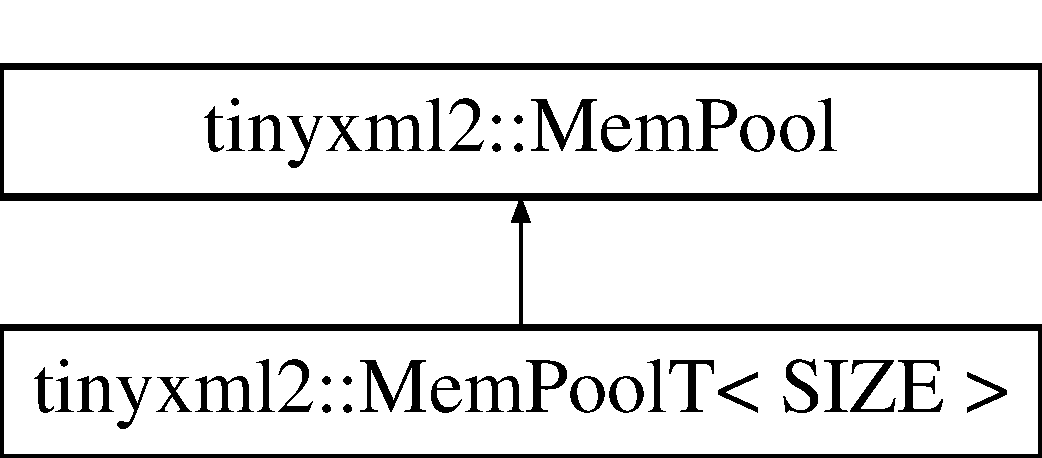
\includegraphics[height=2.000000cm]{classtinyxml2_1_1_mem_pool_t}
\end{center}
\end{figure}
\subsection*{Public Types}
\begin{DoxyCompactItemize}
\item 
enum \{ \hyperlink{classtinyxml2_1_1_mem_pool_t_a04cf45156e6f913f93972869ff8a1d94a4eeedbaa09fc9968120af6190e9e0988}{C\-O\-U\-N\-T} = (4$\ast$1024)/\-S\-I\-Z\-E
 \}
\end{DoxyCompactItemize}
\subsection*{Public Member Functions}
\begin{DoxyCompactItemize}
\item 
\hyperlink{classtinyxml2_1_1_mem_pool_t_a8a69a269ea72e292dde65309528ef64b}{Mem\-Pool\-T} ()
\item 
\hyperlink{classtinyxml2_1_1_mem_pool_t_ad6bb8346ad5b9a34f8f0051da5e3ed3f}{$\sim$\-Mem\-Pool\-T} ()
\item 
virtual int \hyperlink{classtinyxml2_1_1_mem_pool_t_a7ec8778fe99f6e332615a703be0b48bc}{Item\-Size} () const 
\item 
int \hyperlink{classtinyxml2_1_1_mem_pool_t_a56be11b7db6a7ef00db17088a7769aab}{Current\-Allocs} () const 
\item 
virtual void $\ast$ \hyperlink{classtinyxml2_1_1_mem_pool_t_aa9d785a48ffe6ea1be679bab13464486}{Alloc} ()
\item 
virtual void \hyperlink{classtinyxml2_1_1_mem_pool_t_a4f1a0c434e9e3d7391e5c16ed4ee8c70}{Free} (void $\ast$mem)
\item 
void \hyperlink{classtinyxml2_1_1_mem_pool_t_a0bc596f271e0f139822c534238b3f244}{Trace} (const char $\ast$name)
\item 
void \hyperlink{classtinyxml2_1_1_mem_pool_t_a7798932414916199a1bc0f9c3f368521}{Set\-Tracked} ()
\item 
int \hyperlink{classtinyxml2_1_1_mem_pool_t_a524b90d0edeac41964c06510757dce0f}{Untracked} () const 
\end{DoxyCompactItemize}


\subsection{Detailed Description}
\subsubsection*{template$<$int S\-I\-Z\-E$>$class tinyxml2\-::\-Mem\-Pool\-T$<$ S\-I\-Z\-E $>$}



Definition at line 312 of file tinyxml2.\-hpp.



\subsection{Member Enumeration Documentation}
\hypertarget{classtinyxml2_1_1_mem_pool_t_a04cf45156e6f913f93972869ff8a1d94}{\subsubsection[{anonymous enum}]{\setlength{\rightskip}{0pt plus 5cm}template$<$int S\-I\-Z\-E$>$ anonymous enum}}\label{classtinyxml2_1_1_mem_pool_t_a04cf45156e6f913f93972869ff8a1d94}
\begin{Desc}
\item[Enumerator]\par
\begin{description}
\index{C\-O\-U\-N\-T@{C\-O\-U\-N\-T}!tinyxml2\-::\-Mem\-Pool\-T@{tinyxml2\-::\-Mem\-Pool\-T}}\index{tinyxml2\-::\-Mem\-Pool\-T@{tinyxml2\-::\-Mem\-Pool\-T}!C\-O\-U\-N\-T@{C\-O\-U\-N\-T}}\item[{\em 
\hypertarget{classtinyxml2_1_1_mem_pool_t_a04cf45156e6f913f93972869ff8a1d94a4eeedbaa09fc9968120af6190e9e0988}{C\-O\-U\-N\-T}\label{classtinyxml2_1_1_mem_pool_t_a04cf45156e6f913f93972869ff8a1d94a4eeedbaa09fc9968120af6190e9e0988}
}]\end{description}
\end{Desc}


Definition at line 387 of file tinyxml2.\-hpp.



\subsection{Constructor \& Destructor Documentation}
\hypertarget{classtinyxml2_1_1_mem_pool_t_a8a69a269ea72e292dde65309528ef64b}{\index{tinyxml2\-::\-Mem\-Pool\-T@{tinyxml2\-::\-Mem\-Pool\-T}!Mem\-Pool\-T@{Mem\-Pool\-T}}
\index{Mem\-Pool\-T@{Mem\-Pool\-T}!tinyxml2::MemPoolT@{tinyxml2\-::\-Mem\-Pool\-T}}
\subsubsection[{Mem\-Pool\-T}]{\setlength{\rightskip}{0pt plus 5cm}template$<$int S\-I\-Z\-E$>$ {\bf tinyxml2\-::\-Mem\-Pool\-T}$<$ S\-I\-Z\-E $>$\-::{\bf Mem\-Pool\-T} (
\begin{DoxyParamCaption}
{}
\end{DoxyParamCaption}
)\hspace{0.3cm}{\ttfamily [inline]}}}\label{classtinyxml2_1_1_mem_pool_t_a8a69a269ea72e292dde65309528ef64b}


Definition at line 315 of file tinyxml2.\-hpp.

\hypertarget{classtinyxml2_1_1_mem_pool_t_ad6bb8346ad5b9a34f8f0051da5e3ed3f}{\index{tinyxml2\-::\-Mem\-Pool\-T@{tinyxml2\-::\-Mem\-Pool\-T}!$\sim$\-Mem\-Pool\-T@{$\sim$\-Mem\-Pool\-T}}
\index{$\sim$\-Mem\-Pool\-T@{$\sim$\-Mem\-Pool\-T}!tinyxml2::MemPoolT@{tinyxml2\-::\-Mem\-Pool\-T}}
\subsubsection[{$\sim$\-Mem\-Pool\-T}]{\setlength{\rightskip}{0pt plus 5cm}template$<$int S\-I\-Z\-E$>$ {\bf tinyxml2\-::\-Mem\-Pool\-T}$<$ S\-I\-Z\-E $>$\-::$\sim${\bf Mem\-Pool\-T} (
\begin{DoxyParamCaption}
{}
\end{DoxyParamCaption}
)\hspace{0.3cm}{\ttfamily [inline]}}}\label{classtinyxml2_1_1_mem_pool_t_ad6bb8346ad5b9a34f8f0051da5e3ed3f}


Definition at line 316 of file tinyxml2.\-hpp.



\subsection{Member Function Documentation}
\hypertarget{classtinyxml2_1_1_mem_pool_t_aa9d785a48ffe6ea1be679bab13464486}{\index{tinyxml2\-::\-Mem\-Pool\-T@{tinyxml2\-::\-Mem\-Pool\-T}!Alloc@{Alloc}}
\index{Alloc@{Alloc}!tinyxml2::MemPoolT@{tinyxml2\-::\-Mem\-Pool\-T}}
\subsubsection[{Alloc}]{\setlength{\rightskip}{0pt plus 5cm}template$<$int S\-I\-Z\-E$>$ virtual void$\ast$ {\bf tinyxml2\-::\-Mem\-Pool\-T}$<$ S\-I\-Z\-E $>$\-::Alloc (
\begin{DoxyParamCaption}
{}
\end{DoxyParamCaption}
)\hspace{0.3cm}{\ttfamily [inline]}, {\ttfamily [virtual]}}}\label{classtinyxml2_1_1_mem_pool_t_aa9d785a48ffe6ea1be679bab13464486}


Implements \hyperlink{classtinyxml2_1_1_mem_pool_a4f977b5fed752c0bbfe5295f469d6449}{tinyxml2\-::\-Mem\-Pool}.



Definition at line 330 of file tinyxml2.\-hpp.

\hypertarget{classtinyxml2_1_1_mem_pool_t_a56be11b7db6a7ef00db17088a7769aab}{\index{tinyxml2\-::\-Mem\-Pool\-T@{tinyxml2\-::\-Mem\-Pool\-T}!Current\-Allocs@{Current\-Allocs}}
\index{Current\-Allocs@{Current\-Allocs}!tinyxml2::MemPoolT@{tinyxml2\-::\-Mem\-Pool\-T}}
\subsubsection[{Current\-Allocs}]{\setlength{\rightskip}{0pt plus 5cm}template$<$int S\-I\-Z\-E$>$ int {\bf tinyxml2\-::\-Mem\-Pool\-T}$<$ S\-I\-Z\-E $>$\-::Current\-Allocs (
\begin{DoxyParamCaption}
{}
\end{DoxyParamCaption}
) const\hspace{0.3cm}{\ttfamily [inline]}}}\label{classtinyxml2_1_1_mem_pool_t_a56be11b7db6a7ef00db17088a7769aab}


Definition at line 326 of file tinyxml2.\-hpp.

\hypertarget{classtinyxml2_1_1_mem_pool_t_a4f1a0c434e9e3d7391e5c16ed4ee8c70}{\index{tinyxml2\-::\-Mem\-Pool\-T@{tinyxml2\-::\-Mem\-Pool\-T}!Free@{Free}}
\index{Free@{Free}!tinyxml2::MemPoolT@{tinyxml2\-::\-Mem\-Pool\-T}}
\subsubsection[{Free}]{\setlength{\rightskip}{0pt plus 5cm}template$<$int S\-I\-Z\-E$>$ virtual void {\bf tinyxml2\-::\-Mem\-Pool\-T}$<$ S\-I\-Z\-E $>$\-::Free (
\begin{DoxyParamCaption}
\item[{void $\ast$}]{mem}
\end{DoxyParamCaption}
)\hspace{0.3cm}{\ttfamily [inline]}, {\ttfamily [virtual]}}}\label{classtinyxml2_1_1_mem_pool_t_a4f1a0c434e9e3d7391e5c16ed4ee8c70}


Implements \hyperlink{classtinyxml2_1_1_mem_pool_a49e3bfac2cba2ebd6776b31e571f64f7}{tinyxml2\-::\-Mem\-Pool}.



Definition at line 353 of file tinyxml2.\-hpp.

\hypertarget{classtinyxml2_1_1_mem_pool_t_a7ec8778fe99f6e332615a703be0b48bc}{\index{tinyxml2\-::\-Mem\-Pool\-T@{tinyxml2\-::\-Mem\-Pool\-T}!Item\-Size@{Item\-Size}}
\index{Item\-Size@{Item\-Size}!tinyxml2::MemPoolT@{tinyxml2\-::\-Mem\-Pool\-T}}
\subsubsection[{Item\-Size}]{\setlength{\rightskip}{0pt plus 5cm}template$<$int S\-I\-Z\-E$>$ virtual int {\bf tinyxml2\-::\-Mem\-Pool\-T}$<$ S\-I\-Z\-E $>$\-::Item\-Size (
\begin{DoxyParamCaption}
{}
\end{DoxyParamCaption}
) const\hspace{0.3cm}{\ttfamily [inline]}, {\ttfamily [virtual]}}}\label{classtinyxml2_1_1_mem_pool_t_a7ec8778fe99f6e332615a703be0b48bc}


Implements \hyperlink{classtinyxml2_1_1_mem_pool_a0c518d49e3a94bde566f61e13b7240bb}{tinyxml2\-::\-Mem\-Pool}.



Definition at line 323 of file tinyxml2.\-hpp.

\hypertarget{classtinyxml2_1_1_mem_pool_t_a7798932414916199a1bc0f9c3f368521}{\index{tinyxml2\-::\-Mem\-Pool\-T@{tinyxml2\-::\-Mem\-Pool\-T}!Set\-Tracked@{Set\-Tracked}}
\index{Set\-Tracked@{Set\-Tracked}!tinyxml2::MemPoolT@{tinyxml2\-::\-Mem\-Pool\-T}}
\subsubsection[{Set\-Tracked}]{\setlength{\rightskip}{0pt plus 5cm}template$<$int S\-I\-Z\-E$>$ void {\bf tinyxml2\-::\-Mem\-Pool\-T}$<$ S\-I\-Z\-E $>$\-::Set\-Tracked (
\begin{DoxyParamCaption}
{}
\end{DoxyParamCaption}
)\hspace{0.3cm}{\ttfamily [inline]}, {\ttfamily [virtual]}}}\label{classtinyxml2_1_1_mem_pool_t_a7798932414916199a1bc0f9c3f368521}


Implements \hyperlink{classtinyxml2_1_1_mem_pool_ac5804dd1387b2e4de5eef710076a0db1}{tinyxml2\-::\-Mem\-Pool}.



Definition at line 370 of file tinyxml2.\-hpp.

\hypertarget{classtinyxml2_1_1_mem_pool_t_a0bc596f271e0f139822c534238b3f244}{\index{tinyxml2\-::\-Mem\-Pool\-T@{tinyxml2\-::\-Mem\-Pool\-T}!Trace@{Trace}}
\index{Trace@{Trace}!tinyxml2::MemPoolT@{tinyxml2\-::\-Mem\-Pool\-T}}
\subsubsection[{Trace}]{\setlength{\rightskip}{0pt plus 5cm}template$<$int S\-I\-Z\-E$>$ void {\bf tinyxml2\-::\-Mem\-Pool\-T}$<$ S\-I\-Z\-E $>$\-::Trace (
\begin{DoxyParamCaption}
\item[{const char $\ast$}]{name}
\end{DoxyParamCaption}
)\hspace{0.3cm}{\ttfamily [inline]}}}\label{classtinyxml2_1_1_mem_pool_t_a0bc596f271e0f139822c534238b3f244}


Definition at line 365 of file tinyxml2.\-hpp.

\hypertarget{classtinyxml2_1_1_mem_pool_t_a524b90d0edeac41964c06510757dce0f}{\index{tinyxml2\-::\-Mem\-Pool\-T@{tinyxml2\-::\-Mem\-Pool\-T}!Untracked@{Untracked}}
\index{Untracked@{Untracked}!tinyxml2::MemPoolT@{tinyxml2\-::\-Mem\-Pool\-T}}
\subsubsection[{Untracked}]{\setlength{\rightskip}{0pt plus 5cm}template$<$int S\-I\-Z\-E$>$ int {\bf tinyxml2\-::\-Mem\-Pool\-T}$<$ S\-I\-Z\-E $>$\-::Untracked (
\begin{DoxyParamCaption}
{}
\end{DoxyParamCaption}
) const\hspace{0.3cm}{\ttfamily [inline]}}}\label{classtinyxml2_1_1_mem_pool_t_a524b90d0edeac41964c06510757dce0f}


Definition at line 374 of file tinyxml2.\-hpp.



The documentation for this class was generated from the following file\-:\begin{DoxyCompactItemize}
\item 
/home/chris/\-Projects/\-Sudden\-Awakening/\-Source/\hyperlink{tinyxml2_8hpp}{tinyxml2.\-hpp}\end{DoxyCompactItemize}

\hypertarget{class_player}{\section{Player Class Reference}
\label{class_player}\index{Player@{Player}}
}


The \hyperlink{class_player}{Player} class, is the class that holds the data for the player.  




{\ttfamily \#include $<$Entity.\-hpp$>$}

Inheritance diagram for Player\-:\begin{figure}[H]
\begin{center}
\leavevmode
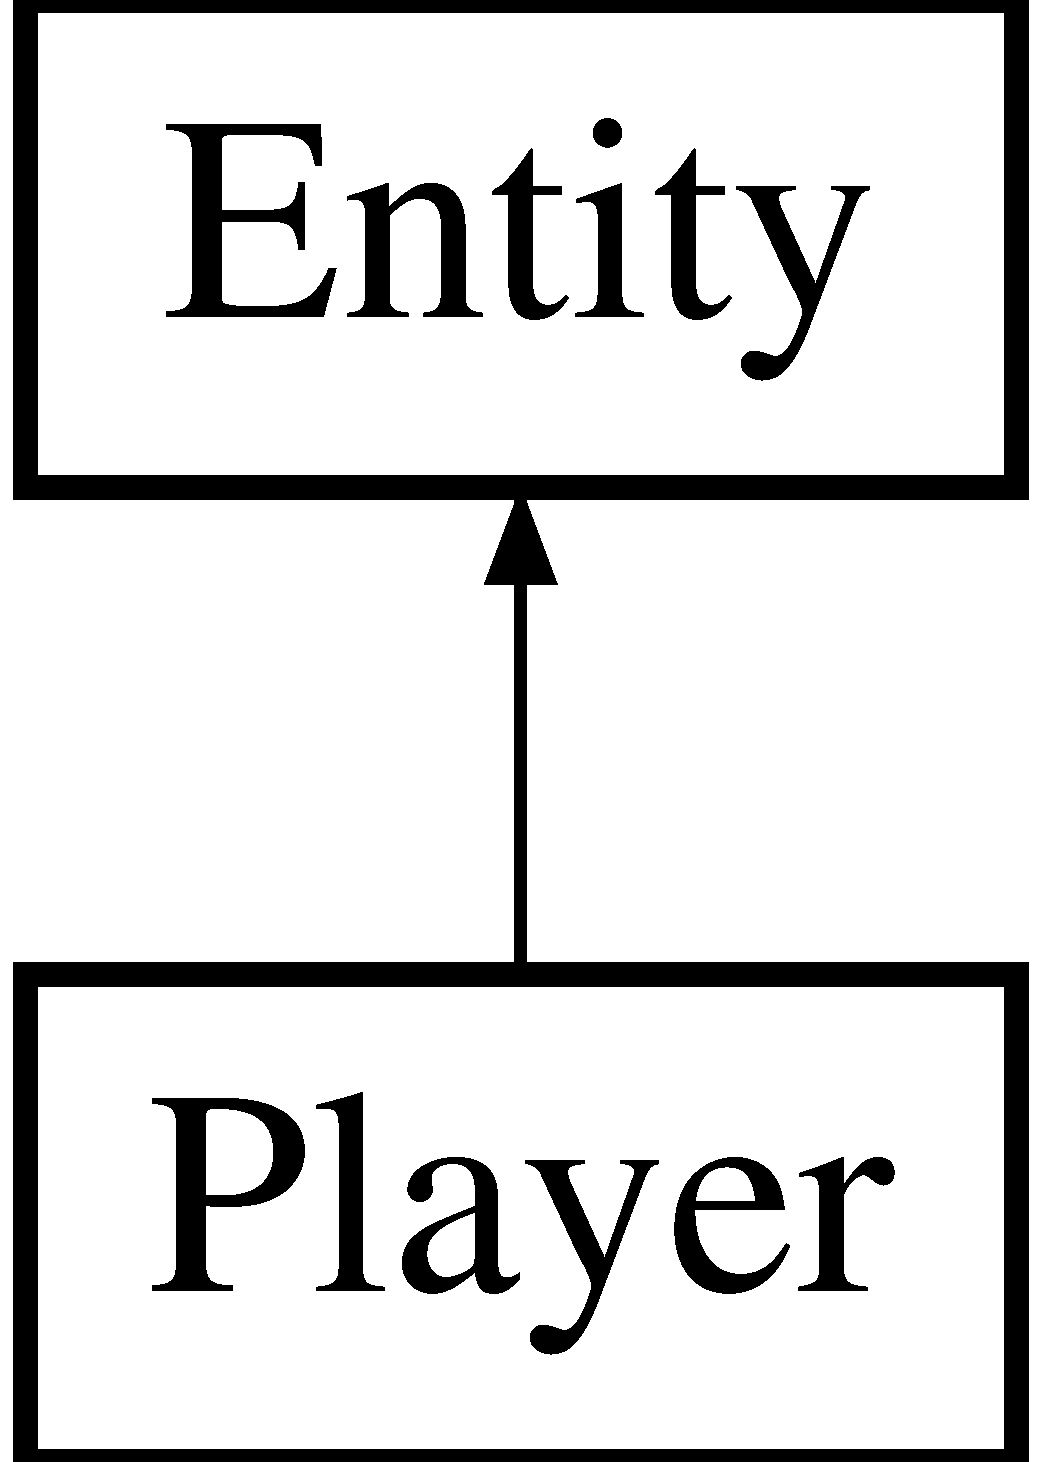
\includegraphics[height=2.000000cm]{class_player}
\end{center}
\end{figure}
\subsection*{Public Member Functions}
\begin{DoxyCompactItemize}
\item 
\hyperlink{class_player_a154b6b768b9a1541d29873affd36af85}{Player} (const sf\-::\-Texture \&texture, const sf\-::\-Vector2f \&pos)
\begin{DoxyCompactList}\small\item\em \hyperlink{class_player}{Player} ctor. \end{DoxyCompactList}\item 
virtual \hyperlink{class_player_a749d2c00e1fe0f5c2746f7505a58c062}{$\sim$\-Player} ()
\begin{DoxyCompactList}\small\item\em $\sim$\-Player virtual call to dtor. \end{DoxyCompactList}\item 
virtual void \hyperlink{class_player_a05b60cac1922c5be5c1be16baffa4497}{Update} ()
\begin{DoxyCompactList}\small\item\em Update, currently empty. \end{DoxyCompactList}\item 
virtual void \hyperlink{class_player_aee32aba0a12ace035c1fc0f3acfa31ca}{Update\-Controls} ()
\begin{DoxyCompactList}\small\item\em Update\-Controls is empty, code moved to \hyperlink{class_level}{Level} class. \end{DoxyCompactList}\item 
int \hyperlink{class_player_a63b37d8526ab108d420f59daa8b456ab}{Get\-X\-Coord} () const 
\begin{DoxyCompactList}\small\item\em Get\-X\-Coord getter for the x coordinate of the current frame. \end{DoxyCompactList}\item 
void \hyperlink{class_player_a171909ce2bc5ad4ed7bd1e329818f1cb}{Set\-X\-Coord} (int x\-Coord)
\begin{DoxyCompactList}\small\item\em Set\-X\-Coord setter for the x coordinate of the current frame. \end{DoxyCompactList}\item 
int \hyperlink{class_player_a7ea86222c187ffc350e4948e3d82459e}{Get\-Y\-Coord} () const 
\begin{DoxyCompactList}\small\item\em Get\-Y\-Coord getter for the y coordinate of the current frame. \end{DoxyCompactList}\item 
void \hyperlink{class_player_ae2b9268a010501d169798c201be0aea0}{Set\-Y\-Coord} (int y\-Coord)
\begin{DoxyCompactList}\small\item\em Set\-Y\-Coord. \end{DoxyCompactList}\item 
int \hyperlink{class_player_a0b6c9a9030fe30e04bd00f423d617b72}{Get\-X\-Direction} () const 
\begin{DoxyCompactList}\small\item\em Get\-X\-Direction getter for the direction of the animation either +-\/ 1 to indicate direction. \end{DoxyCompactList}\item 
void \hyperlink{class_player_ad1d525ce156cc87325d671faa537c644}{Set\-X\-Direction} (int x\-Direction)
\begin{DoxyCompactList}\small\item\em Set\-X\-Direction setter for the direction of the animation either +-\/ 1 to indicate direction. \end{DoxyCompactList}\item 
int \hyperlink{class_player_afd3cdd13b6de01c1a52ce47a5871df65}{Get\-Texture\-Sheet\-Width} () const 
\begin{DoxyCompactList}\small\item\em Get\-Texture\-Sheet\-Width getter for the texture sheets width. \end{DoxyCompactList}\item 
int \hyperlink{class_player_adbce7ab22e580ba85cd9a3fddac9695f}{Get\-Texture\-Sheet\-Height} () const 
\begin{DoxyCompactList}\small\item\em Get\-Texture\-Sheet\-Height getter for the texture sheets height. \end{DoxyCompactList}\item 
\hyperlink{_game_8hpp_a332b72dfb4bc8b4c16b8dc43864fe343}{Time\-Int} \hyperlink{class_player_a8cf47bf652a24ea4826c04810251e332}{Get\-Next\-Frame\-Trigger} () const 
\begin{DoxyCompactList}\small\item\em Get\-Next\-Frame\-Trigger get the time until the next frame should be displayed. \end{DoxyCompactList}\item 
void \hyperlink{class_player_a34ee83b70e69a08c2f397a05ab6421b9}{Set\-Next\-Frame\-Trigger} (\hyperlink{_game_8hpp_a332b72dfb4bc8b4c16b8dc43864fe343}{Time\-Int} trigger)
\begin{DoxyCompactList}\small\item\em Set\-Next\-Frame\-Trigger setter for the time until the next frame should be displayed. \end{DoxyCompactList}\end{DoxyCompactItemize}
\subsection*{Protected Attributes}
\begin{DoxyCompactItemize}
\item 
int \hyperlink{class_player_ab5f657ba805e70319fc312533d715d96}{m\-Xcoord}
\item 
int \hyperlink{class_player_ab3a89b65abf92da672ebc3c55b22dc80}{m\-Ycoord}
\item 
int \hyperlink{class_player_a141ca66b2ec828bb84617b21dc7e9db0}{m\-X\-Direction}
\item 
int \hyperlink{class_player_abdccfacdffb3a21371af39dbe0255453}{m\-Texture\-Sheet\-Width}
\item 
int \hyperlink{class_player_a9d15c816285b1708e3a93ef41a628263}{m\-Texture\-Sheet\-Height}
\item 
int \hyperlink{class_player_a8edce47b376093a95a89c91eee9b253e}{m\-Map\-Tile\-Size}
\item 
\hyperlink{_game_8hpp_a332b72dfb4bc8b4c16b8dc43864fe343}{Time\-Int} \hyperlink{class_player_a97ef6ab1b525c97f0e4fdd9ece101b03}{m\-Next\-Frame\-Trigger}
\end{DoxyCompactItemize}


\subsection{Detailed Description}
The \hyperlink{class_player}{Player} class, is the class that holds the data for the player. 

It inherits from \hyperlink{class_entity}{Entity}

This class is capable of animating itself. It can be moved around the screen. Other than that not much else functionality.

The animation works by tracking the frames in x and y.

You then multiply the tile size by the coordinate frame. So x\-Coord $\ast$ tile\-Size = position of frame in x on the texture. 

Definition at line 139 of file Entity.\-hpp.



\subsection{Constructor \& Destructor Documentation}
\hypertarget{class_player_a154b6b768b9a1541d29873affd36af85}{\index{Player@{Player}!Player@{Player}}
\index{Player@{Player}!Player@{Player}}
\subsubsection[{Player}]{\setlength{\rightskip}{0pt plus 5cm}Player\-::\-Player (
\begin{DoxyParamCaption}
\item[{const sf\-::\-Texture \&}]{texture, }
\item[{const sf\-::\-Vector2f \&}]{pos}
\end{DoxyParamCaption}
)}}\label{class_player_a154b6b768b9a1541d29873affd36af85}


\hyperlink{class_player}{Player} ctor. 


\begin{DoxyParams}{Parameters}
{\em texture} & The sf\-::\-Texture to use as the players representation. \\
\hline
{\em pos} & The initial position of the player. \\
\hline
\end{DoxyParams}


Definition at line 97 of file Entity.\-cpp.

\hypertarget{class_player_a749d2c00e1fe0f5c2746f7505a58c062}{\index{Player@{Player}!$\sim$\-Player@{$\sim$\-Player}}
\index{$\sim$\-Player@{$\sim$\-Player}!Player@{Player}}
\subsubsection[{$\sim$\-Player}]{\setlength{\rightskip}{0pt plus 5cm}Player\-::$\sim$\-Player (
\begin{DoxyParamCaption}
{}
\end{DoxyParamCaption}
)\hspace{0.3cm}{\ttfamily [virtual]}}}\label{class_player_a749d2c00e1fe0f5c2746f7505a58c062}


$\sim$\-Player virtual call to dtor. 



Definition at line 128 of file Entity.\-cpp.



\subsection{Member Function Documentation}
\hypertarget{class_player_a8cf47bf652a24ea4826c04810251e332}{\index{Player@{Player}!Get\-Next\-Frame\-Trigger@{Get\-Next\-Frame\-Trigger}}
\index{Get\-Next\-Frame\-Trigger@{Get\-Next\-Frame\-Trigger}!Player@{Player}}
\subsubsection[{Get\-Next\-Frame\-Trigger}]{\setlength{\rightskip}{0pt plus 5cm}{\bf Time\-Int} Player\-::\-Get\-Next\-Frame\-Trigger (
\begin{DoxyParamCaption}
{}
\end{DoxyParamCaption}
) const}}\label{class_player_a8cf47bf652a24ea4826c04810251e332}


Get\-Next\-Frame\-Trigger get the time until the next frame should be displayed. 

\begin{DoxyReturn}{Returns}
The time until the next frame should be displayed. 
\end{DoxyReturn}


Definition at line 183 of file Entity.\-cpp.

\hypertarget{class_player_adbce7ab22e580ba85cd9a3fddac9695f}{\index{Player@{Player}!Get\-Texture\-Sheet\-Height@{Get\-Texture\-Sheet\-Height}}
\index{Get\-Texture\-Sheet\-Height@{Get\-Texture\-Sheet\-Height}!Player@{Player}}
\subsubsection[{Get\-Texture\-Sheet\-Height}]{\setlength{\rightskip}{0pt plus 5cm}int Player\-::\-Get\-Texture\-Sheet\-Height (
\begin{DoxyParamCaption}
{}
\end{DoxyParamCaption}
) const}}\label{class_player_adbce7ab22e580ba85cd9a3fddac9695f}


Get\-Texture\-Sheet\-Height getter for the texture sheets height. 

\begin{DoxyReturn}{Returns}
The texture sheets height. 
\end{DoxyReturn}


Definition at line 178 of file Entity.\-cpp.

\hypertarget{class_player_afd3cdd13b6de01c1a52ce47a5871df65}{\index{Player@{Player}!Get\-Texture\-Sheet\-Width@{Get\-Texture\-Sheet\-Width}}
\index{Get\-Texture\-Sheet\-Width@{Get\-Texture\-Sheet\-Width}!Player@{Player}}
\subsubsection[{Get\-Texture\-Sheet\-Width}]{\setlength{\rightskip}{0pt plus 5cm}int Player\-::\-Get\-Texture\-Sheet\-Width (
\begin{DoxyParamCaption}
{}
\end{DoxyParamCaption}
) const}}\label{class_player_afd3cdd13b6de01c1a52ce47a5871df65}


Get\-Texture\-Sheet\-Width getter for the texture sheets width. 

\begin{DoxyReturn}{Returns}
The texture sheets width. 
\end{DoxyReturn}


Definition at line 173 of file Entity.\-cpp.

\hypertarget{class_player_a63b37d8526ab108d420f59daa8b456ab}{\index{Player@{Player}!Get\-X\-Coord@{Get\-X\-Coord}}
\index{Get\-X\-Coord@{Get\-X\-Coord}!Player@{Player}}
\subsubsection[{Get\-X\-Coord}]{\setlength{\rightskip}{0pt plus 5cm}int Player\-::\-Get\-X\-Coord (
\begin{DoxyParamCaption}
{}
\end{DoxyParamCaption}
) const}}\label{class_player_a63b37d8526ab108d420f59daa8b456ab}


Get\-X\-Coord getter for the x coordinate of the current frame. 

\begin{DoxyReturn}{Returns}
The current x frame coordinate. 
\end{DoxyReturn}


Definition at line 143 of file Entity.\-cpp.

\hypertarget{class_player_a0b6c9a9030fe30e04bd00f423d617b72}{\index{Player@{Player}!Get\-X\-Direction@{Get\-X\-Direction}}
\index{Get\-X\-Direction@{Get\-X\-Direction}!Player@{Player}}
\subsubsection[{Get\-X\-Direction}]{\setlength{\rightskip}{0pt plus 5cm}int Player\-::\-Get\-X\-Direction (
\begin{DoxyParamCaption}
{}
\end{DoxyParamCaption}
) const}}\label{class_player_a0b6c9a9030fe30e04bd00f423d617b72}


Get\-X\-Direction getter for the direction of the animation either +-\/ 1 to indicate direction. 

\begin{DoxyReturn}{Returns}
The value to indicate animation direction. 
\end{DoxyReturn}


Definition at line 163 of file Entity.\-cpp.

\hypertarget{class_player_a7ea86222c187ffc350e4948e3d82459e}{\index{Player@{Player}!Get\-Y\-Coord@{Get\-Y\-Coord}}
\index{Get\-Y\-Coord@{Get\-Y\-Coord}!Player@{Player}}
\subsubsection[{Get\-Y\-Coord}]{\setlength{\rightskip}{0pt plus 5cm}int Player\-::\-Get\-Y\-Coord (
\begin{DoxyParamCaption}
{}
\end{DoxyParamCaption}
) const}}\label{class_player_a7ea86222c187ffc350e4948e3d82459e}


Get\-Y\-Coord getter for the y coordinate of the current frame. 

\begin{DoxyReturn}{Returns}
The current y frame coordinate. 
\end{DoxyReturn}


Definition at line 153 of file Entity.\-cpp.

\hypertarget{class_player_a34ee83b70e69a08c2f397a05ab6421b9}{\index{Player@{Player}!Set\-Next\-Frame\-Trigger@{Set\-Next\-Frame\-Trigger}}
\index{Set\-Next\-Frame\-Trigger@{Set\-Next\-Frame\-Trigger}!Player@{Player}}
\subsubsection[{Set\-Next\-Frame\-Trigger}]{\setlength{\rightskip}{0pt plus 5cm}void Player\-::\-Set\-Next\-Frame\-Trigger (
\begin{DoxyParamCaption}
\item[{{\bf Time\-Int}}]{trigger}
\end{DoxyParamCaption}
)}}\label{class_player_a34ee83b70e69a08c2f397a05ab6421b9}


Set\-Next\-Frame\-Trigger setter for the time until the next frame should be displayed. 


\begin{DoxyParams}{Parameters}
{\em trigger} & The time until the next frame should be displayed. \\
\hline
\end{DoxyParams}


Definition at line 188 of file Entity.\-cpp.

\hypertarget{class_player_a171909ce2bc5ad4ed7bd1e329818f1cb}{\index{Player@{Player}!Set\-X\-Coord@{Set\-X\-Coord}}
\index{Set\-X\-Coord@{Set\-X\-Coord}!Player@{Player}}
\subsubsection[{Set\-X\-Coord}]{\setlength{\rightskip}{0pt plus 5cm}void Player\-::\-Set\-X\-Coord (
\begin{DoxyParamCaption}
\item[{int}]{x\-Coord}
\end{DoxyParamCaption}
)}}\label{class_player_a171909ce2bc5ad4ed7bd1e329818f1cb}


Set\-X\-Coord setter for the x coordinate of the current frame. 


\begin{DoxyParams}{Parameters}
{\em x\-Coord} & The value to set as the new frame. \\
\hline
\end{DoxyParams}


Definition at line 148 of file Entity.\-cpp.

\hypertarget{class_player_ad1d525ce156cc87325d671faa537c644}{\index{Player@{Player}!Set\-X\-Direction@{Set\-X\-Direction}}
\index{Set\-X\-Direction@{Set\-X\-Direction}!Player@{Player}}
\subsubsection[{Set\-X\-Direction}]{\setlength{\rightskip}{0pt plus 5cm}void Player\-::\-Set\-X\-Direction (
\begin{DoxyParamCaption}
\item[{int}]{x\-Direction}
\end{DoxyParamCaption}
)}}\label{class_player_ad1d525ce156cc87325d671faa537c644}


Set\-X\-Direction setter for the direction of the animation either +-\/ 1 to indicate direction. 


\begin{DoxyParams}{Parameters}
{\em x\-Direction} & The value to set as the animation direction. \\
\hline
\end{DoxyParams}


Definition at line 168 of file Entity.\-cpp.

\hypertarget{class_player_ae2b9268a010501d169798c201be0aea0}{\index{Player@{Player}!Set\-Y\-Coord@{Set\-Y\-Coord}}
\index{Set\-Y\-Coord@{Set\-Y\-Coord}!Player@{Player}}
\subsubsection[{Set\-Y\-Coord}]{\setlength{\rightskip}{0pt plus 5cm}void Player\-::\-Set\-Y\-Coord (
\begin{DoxyParamCaption}
\item[{int}]{y\-Coord}
\end{DoxyParamCaption}
)}}\label{class_player_ae2b9268a010501d169798c201be0aea0}


Set\-Y\-Coord. 


\begin{DoxyParams}{Parameters}
{\em y\-Coord} & \\
\hline
\end{DoxyParams}


Definition at line 158 of file Entity.\-cpp.

\hypertarget{class_player_a05b60cac1922c5be5c1be16baffa4497}{\index{Player@{Player}!Update@{Update}}
\index{Update@{Update}!Player@{Player}}
\subsubsection[{Update}]{\setlength{\rightskip}{0pt plus 5cm}void Player\-::\-Update (
\begin{DoxyParamCaption}
{}
\end{DoxyParamCaption}
)\hspace{0.3cm}{\ttfamily [virtual]}}}\label{class_player_a05b60cac1922c5be5c1be16baffa4497}


Update, currently empty. 



Reimplemented from \hyperlink{class_entity_a7e2a7c5df3bceaf41deea192eeba4d8f}{Entity}.



Definition at line 133 of file Entity.\-cpp.

\hypertarget{class_player_aee32aba0a12ace035c1fc0f3acfa31ca}{\index{Player@{Player}!Update\-Controls@{Update\-Controls}}
\index{Update\-Controls@{Update\-Controls}!Player@{Player}}
\subsubsection[{Update\-Controls}]{\setlength{\rightskip}{0pt plus 5cm}void Player\-::\-Update\-Controls (
\begin{DoxyParamCaption}
{}
\end{DoxyParamCaption}
)\hspace{0.3cm}{\ttfamily [virtual]}}}\label{class_player_aee32aba0a12ace035c1fc0f3acfa31ca}


Update\-Controls is empty, code moved to \hyperlink{class_level}{Level} class. 



Definition at line 138 of file Entity.\-cpp.



\subsection{Member Data Documentation}
\hypertarget{class_player_a8edce47b376093a95a89c91eee9b253e}{\index{Player@{Player}!m\-Map\-Tile\-Size@{m\-Map\-Tile\-Size}}
\index{m\-Map\-Tile\-Size@{m\-Map\-Tile\-Size}!Player@{Player}}
\subsubsection[{m\-Map\-Tile\-Size}]{\setlength{\rightskip}{0pt plus 5cm}int Player\-::m\-Map\-Tile\-Size\hspace{0.3cm}{\ttfamily [protected]}}}\label{class_player_a8edce47b376093a95a89c91eee9b253e}


Definition at line 233 of file Entity.\-hpp.

\hypertarget{class_player_a97ef6ab1b525c97f0e4fdd9ece101b03}{\index{Player@{Player}!m\-Next\-Frame\-Trigger@{m\-Next\-Frame\-Trigger}}
\index{m\-Next\-Frame\-Trigger@{m\-Next\-Frame\-Trigger}!Player@{Player}}
\subsubsection[{m\-Next\-Frame\-Trigger}]{\setlength{\rightskip}{0pt plus 5cm}{\bf Time\-Int} Player\-::m\-Next\-Frame\-Trigger\hspace{0.3cm}{\ttfamily [protected]}}}\label{class_player_a97ef6ab1b525c97f0e4fdd9ece101b03}


Definition at line 235 of file Entity.\-hpp.

\hypertarget{class_player_a9d15c816285b1708e3a93ef41a628263}{\index{Player@{Player}!m\-Texture\-Sheet\-Height@{m\-Texture\-Sheet\-Height}}
\index{m\-Texture\-Sheet\-Height@{m\-Texture\-Sheet\-Height}!Player@{Player}}
\subsubsection[{m\-Texture\-Sheet\-Height}]{\setlength{\rightskip}{0pt plus 5cm}int Player\-::m\-Texture\-Sheet\-Height\hspace{0.3cm}{\ttfamily [protected]}}}\label{class_player_a9d15c816285b1708e3a93ef41a628263}


Definition at line 231 of file Entity.\-hpp.

\hypertarget{class_player_abdccfacdffb3a21371af39dbe0255453}{\index{Player@{Player}!m\-Texture\-Sheet\-Width@{m\-Texture\-Sheet\-Width}}
\index{m\-Texture\-Sheet\-Width@{m\-Texture\-Sheet\-Width}!Player@{Player}}
\subsubsection[{m\-Texture\-Sheet\-Width}]{\setlength{\rightskip}{0pt plus 5cm}int Player\-::m\-Texture\-Sheet\-Width\hspace{0.3cm}{\ttfamily [protected]}}}\label{class_player_abdccfacdffb3a21371af39dbe0255453}


Definition at line 230 of file Entity.\-hpp.

\hypertarget{class_player_ab5f657ba805e70319fc312533d715d96}{\index{Player@{Player}!m\-Xcoord@{m\-Xcoord}}
\index{m\-Xcoord@{m\-Xcoord}!Player@{Player}}
\subsubsection[{m\-Xcoord}]{\setlength{\rightskip}{0pt plus 5cm}int Player\-::m\-Xcoord\hspace{0.3cm}{\ttfamily [protected]}}}\label{class_player_ab5f657ba805e70319fc312533d715d96}


Definition at line 225 of file Entity.\-hpp.

\hypertarget{class_player_a141ca66b2ec828bb84617b21dc7e9db0}{\index{Player@{Player}!m\-X\-Direction@{m\-X\-Direction}}
\index{m\-X\-Direction@{m\-X\-Direction}!Player@{Player}}
\subsubsection[{m\-X\-Direction}]{\setlength{\rightskip}{0pt plus 5cm}int Player\-::m\-X\-Direction\hspace{0.3cm}{\ttfamily [protected]}}}\label{class_player_a141ca66b2ec828bb84617b21dc7e9db0}


Definition at line 228 of file Entity.\-hpp.

\hypertarget{class_player_ab3a89b65abf92da672ebc3c55b22dc80}{\index{Player@{Player}!m\-Ycoord@{m\-Ycoord}}
\index{m\-Ycoord@{m\-Ycoord}!Player@{Player}}
\subsubsection[{m\-Ycoord}]{\setlength{\rightskip}{0pt plus 5cm}int Player\-::m\-Ycoord\hspace{0.3cm}{\ttfamily [protected]}}}\label{class_player_ab3a89b65abf92da672ebc3c55b22dc80}


Definition at line 226 of file Entity.\-hpp.



The documentation for this class was generated from the following files\-:\begin{DoxyCompactItemize}
\item 
Source/\hyperlink{_entity_8hpp}{Entity.\-hpp}\item 
Source/\hyperlink{_entity_8cpp}{Entity.\-cpp}\end{DoxyCompactItemize}

\hypertarget{class_resource_manager}{\section{Resource\-Manager$<$ Type $>$ Class Template Reference}
\label{class_resource_manager}\index{Resource\-Manager$<$ Type $>$@{Resource\-Manager$<$ Type $>$}}
}


\hyperlink{class_resource_manager}{Resource\-Manager} is simple class for managing resources.  




{\ttfamily \#include $<$Resource\-Manager.\-hpp$>$}

\subsection*{Public Member Functions}
\begin{DoxyCompactItemize}
\item 
void \hyperlink{class_resource_manager_a38f6162e5f7d3b16273a23340b34e438}{Load\-Resource} (const std\-::string \&file, \hyperlink{_resource_manager_8hpp_adfdcfc7f1686e261462215a5a516110e}{Resource\-I\-D} id)
\begin{DoxyCompactList}\small\item\em Load\-Resource is where resources are loaded and associated with an integer I\-D. \end{DoxyCompactList}\item 
Type \& \hyperlink{class_resource_manager_af3e977ad6ea9972aebf6c7d7c15a19d6}{Get\-Resource} (\hyperlink{_resource_manager_8hpp_adfdcfc7f1686e261462215a5a516110e}{Resource\-I\-D} id) const 
\begin{DoxyCompactList}\small\item\em Get\-Resource is where you can get a reference to a loaded resource. If an I\-D requested was not found it will throw an exception. \end{DoxyCompactList}\item 
void \hyperlink{class_resource_manager_a919997a4e1b07f62181bedad680915aa}{Clear\-All} ()
\begin{DoxyCompactList}\small\item\em Clear\-All immediately destructs all the resources in this manager. \end{DoxyCompactList}\end{DoxyCompactItemize}
\subsection*{Protected Attributes}
\begin{DoxyCompactItemize}
\item 
std\-::map$<$ \hyperlink{_resource_manager_8hpp_adfdcfc7f1686e261462215a5a516110e}{Resource\-I\-D}, \\*
std\-::unique\-\_\-ptr$<$ Type $>$ $>$ \hyperlink{class_resource_manager_af7f7accf221f620d9816ad3cfb80674e}{m\-Resource\-Map}
\end{DoxyCompactItemize}


\subsection{Detailed Description}
\subsubsection*{template$<$typename Type$>$class Resource\-Manager$<$ Type $>$}

\hyperlink{class_resource_manager}{Resource\-Manager} is simple class for managing resources. 

It will take in a file name and path, and an integer I\-D to associate with that resource.

If Load\-Resource loads the resource successfully you may then get a reference to it by calling Get\-Resource(id).

If loading was not successful the class will throw an exception.

Resource I\-Ds should be unique. 

Definition at line 27 of file Resource\-Manager.\-hpp.



\subsection{Member Function Documentation}
\hypertarget{class_resource_manager_a919997a4e1b07f62181bedad680915aa}{\index{Resource\-Manager@{Resource\-Manager}!Clear\-All@{Clear\-All}}
\index{Clear\-All@{Clear\-All}!ResourceManager@{Resource\-Manager}}
\subsubsection[{Clear\-All}]{\setlength{\rightskip}{0pt plus 5cm}template$<$typename Type $>$ void {\bf Resource\-Manager}$<$ Type $>$\-::Clear\-All (
\begin{DoxyParamCaption}
{}
\end{DoxyParamCaption}
)}}\label{class_resource_manager_a919997a4e1b07f62181bedad680915aa}


Clear\-All immediately destructs all the resources in this manager. 



Definition at line 94 of file Resource\-Manager.\-hpp.

\hypertarget{class_resource_manager_af3e977ad6ea9972aebf6c7d7c15a19d6}{\index{Resource\-Manager@{Resource\-Manager}!Get\-Resource@{Get\-Resource}}
\index{Get\-Resource@{Get\-Resource}!ResourceManager@{Resource\-Manager}}
\subsubsection[{Get\-Resource}]{\setlength{\rightskip}{0pt plus 5cm}template$<$typename Type $>$ Type \& {\bf Resource\-Manager}$<$ Type $>$\-::Get\-Resource (
\begin{DoxyParamCaption}
\item[{{\bf Resource\-I\-D}}]{id}
\end{DoxyParamCaption}
) const}}\label{class_resource_manager_af3e977ad6ea9972aebf6c7d7c15a19d6}


Get\-Resource is where you can get a reference to a loaded resource. If an I\-D requested was not found it will throw an exception. 


\begin{DoxyParams}{Parameters}
{\em id} & The integer I\-D requested. \\
\hline
\end{DoxyParams}
\begin{DoxyReturn}{Returns}
A reference to the resource. 
\end{DoxyReturn}


Definition at line 82 of file Resource\-Manager.\-hpp.

\hypertarget{class_resource_manager_a38f6162e5f7d3b16273a23340b34e438}{\index{Resource\-Manager@{Resource\-Manager}!Load\-Resource@{Load\-Resource}}
\index{Load\-Resource@{Load\-Resource}!ResourceManager@{Resource\-Manager}}
\subsubsection[{Load\-Resource}]{\setlength{\rightskip}{0pt plus 5cm}template$<$typename Type $>$ void {\bf Resource\-Manager}$<$ Type $>$\-::Load\-Resource (
\begin{DoxyParamCaption}
\item[{const std\-::string \&}]{file, }
\item[{{\bf Resource\-I\-D}}]{id}
\end{DoxyParamCaption}
)}}\label{class_resource_manager_a38f6162e5f7d3b16273a23340b34e438}


Load\-Resource is where resources are loaded and associated with an integer I\-D. 


\begin{DoxyParams}{Parameters}
{\em file} & The file name and path to the resource for loading. \\
\hline
{\em id} & The integer I\-D to associate with this resource. \\
\hline
\end{DoxyParams}


Definition at line 54 of file Resource\-Manager.\-hpp.



\subsection{Member Data Documentation}
\hypertarget{class_resource_manager_af7f7accf221f620d9816ad3cfb80674e}{\index{Resource\-Manager@{Resource\-Manager}!m\-Resource\-Map@{m\-Resource\-Map}}
\index{m\-Resource\-Map@{m\-Resource\-Map}!ResourceManager@{Resource\-Manager}}
\subsubsection[{m\-Resource\-Map}]{\setlength{\rightskip}{0pt plus 5cm}template$<$typename Type$>$ std\-::map$<${\bf Resource\-I\-D}, std\-::unique\-\_\-ptr$<$Type$>$ $>$ {\bf Resource\-Manager}$<$ Type $>$\-::m\-Resource\-Map\hspace{0.3cm}{\ttfamily [protected]}}}\label{class_resource_manager_af7f7accf221f620d9816ad3cfb80674e}


Definition at line 50 of file Resource\-Manager.\-hpp.



The documentation for this class was generated from the following file\-:\begin{DoxyCompactItemize}
\item 
/home/chris/\-Projects/\-Sudden\-Awakening/\-Source/\hyperlink{_resource_manager_8hpp}{Resource\-Manager.\-hpp}\end{DoxyCompactItemize}

\hypertarget{class_runtime_exception}{\section{Runtime\-Exception Class Reference}
\label{class_runtime_exception}\index{Runtime\-Exception@{Runtime\-Exception}}
}


{\ttfamily \#include $<$Exceptions.\-hpp$>$}

Inheritance diagram for Runtime\-Exception\-:\begin{figure}[H]
\begin{center}
\leavevmode
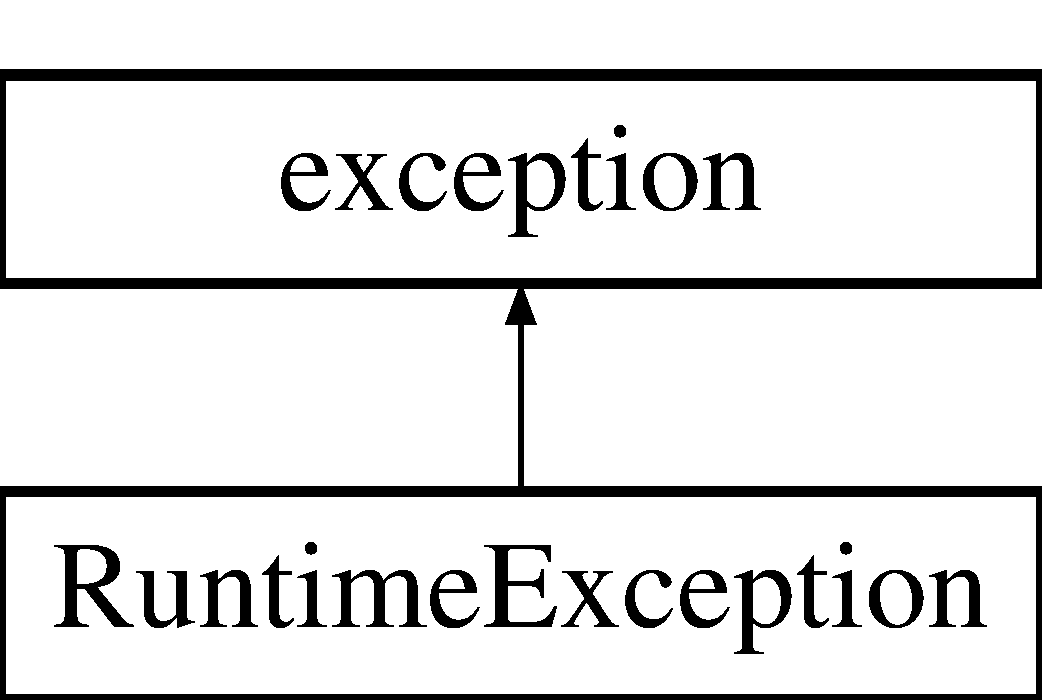
\includegraphics[height=2.000000cm]{class_runtime_exception}
\end{center}
\end{figure}
\subsection*{Public Member Functions}
\begin{DoxyCompactItemize}
\item 
\hyperlink{class_runtime_exception_a74daf11dd2d8f27ce31eb1a20c4bb51d}{Runtime\-Exception} (const std\-::string file, const int line, const std\-::string error\-Desc)
\item 
\hyperlink{class_runtime_exception_a16f5815dc82b7555e90f00a0f903931a}{Runtime\-Exception} (const std\-::string file, const int line, const std\-::string error\-Desc, const std\-::string error\-String, int error\-Code)
\item 
virtual const char $\ast$ \hyperlink{class_runtime_exception_af4bfdc4ed954aada1cee8da317a60a74}{what} () const noexcept
\end{DoxyCompactItemize}
\subsection*{Protected Attributes}
\begin{DoxyCompactItemize}
\item 
std\-::string \hyperlink{class_runtime_exception_a5e945378f1f675427e50ab1f17e0a0f2}{m\-What}
\end{DoxyCompactItemize}


\subsection{Detailed Description}


Definition at line 13 of file Exceptions.\-hpp.



\subsection{Constructor \& Destructor Documentation}
\hypertarget{class_runtime_exception_a74daf11dd2d8f27ce31eb1a20c4bb51d}{\index{Runtime\-Exception@{Runtime\-Exception}!Runtime\-Exception@{Runtime\-Exception}}
\index{Runtime\-Exception@{Runtime\-Exception}!RuntimeException@{Runtime\-Exception}}
\subsubsection[{Runtime\-Exception}]{\setlength{\rightskip}{0pt plus 5cm}Runtime\-Exception\-::\-Runtime\-Exception (
\begin{DoxyParamCaption}
\item[{const std\-::string}]{file, }
\item[{const int}]{line, }
\item[{const std\-::string}]{error\-Desc}
\end{DoxyParamCaption}
)}}\label{class_runtime_exception_a74daf11dd2d8f27ce31eb1a20c4bb51d}


Definition at line 29 of file Exceptions.\-cpp.

\hypertarget{class_runtime_exception_a16f5815dc82b7555e90f00a0f903931a}{\index{Runtime\-Exception@{Runtime\-Exception}!Runtime\-Exception@{Runtime\-Exception}}
\index{Runtime\-Exception@{Runtime\-Exception}!RuntimeException@{Runtime\-Exception}}
\subsubsection[{Runtime\-Exception}]{\setlength{\rightskip}{0pt plus 5cm}Runtime\-Exception\-::\-Runtime\-Exception (
\begin{DoxyParamCaption}
\item[{const std\-::string}]{file, }
\item[{const int}]{line, }
\item[{const std\-::string}]{error\-Desc, }
\item[{const std\-::string}]{error\-String, }
\item[{int}]{error\-Code = {\ttfamily -\/1}}
\end{DoxyParamCaption}
)}}\label{class_runtime_exception_a16f5815dc82b7555e90f00a0f903931a}


Definition at line 37 of file Exceptions.\-cpp.



\subsection{Member Function Documentation}
\hypertarget{class_runtime_exception_af4bfdc4ed954aada1cee8da317a60a74}{\index{Runtime\-Exception@{Runtime\-Exception}!what@{what}}
\index{what@{what}!RuntimeException@{Runtime\-Exception}}
\subsubsection[{what}]{\setlength{\rightskip}{0pt plus 5cm}const char $\ast$ Runtime\-Exception\-::what (
\begin{DoxyParamCaption}
{}
\end{DoxyParamCaption}
) const\hspace{0.3cm}{\ttfamily [virtual]}, {\ttfamily [noexcept]}}}\label{class_runtime_exception_af4bfdc4ed954aada1cee8da317a60a74}


Definition at line 45 of file Exceptions.\-cpp.



\subsection{Member Data Documentation}
\hypertarget{class_runtime_exception_a5e945378f1f675427e50ab1f17e0a0f2}{\index{Runtime\-Exception@{Runtime\-Exception}!m\-What@{m\-What}}
\index{m\-What@{m\-What}!RuntimeException@{Runtime\-Exception}}
\subsubsection[{m\-What}]{\setlength{\rightskip}{0pt plus 5cm}std\-::string Runtime\-Exception\-::m\-What\hspace{0.3cm}{\ttfamily [protected]}}}\label{class_runtime_exception_a5e945378f1f675427e50ab1f17e0a0f2}


Definition at line 22 of file Exceptions.\-hpp.



The documentation for this class was generated from the following files\-:\begin{DoxyCompactItemize}
\item 
/home/chris/\-Projects/\-Sudden\-Awakening/\-Source/\hyperlink{_exceptions_8hpp}{Exceptions.\-hpp}\item 
/home/chris/\-Projects/\-Sudden\-Awakening/\-Source/\hyperlink{_exceptions_8cpp}{Exceptions.\-cpp}\end{DoxyCompactItemize}

\hypertarget{class_state}{\section{State Class Reference}
\label{class_state}\index{State@{State}}
}


The \hyperlink{class_state}{State} class is the base class for states.  




{\ttfamily \#include $<$State.\-hpp$>$}

Inheritance diagram for State\-:\begin{figure}[H]
\begin{center}
\leavevmode
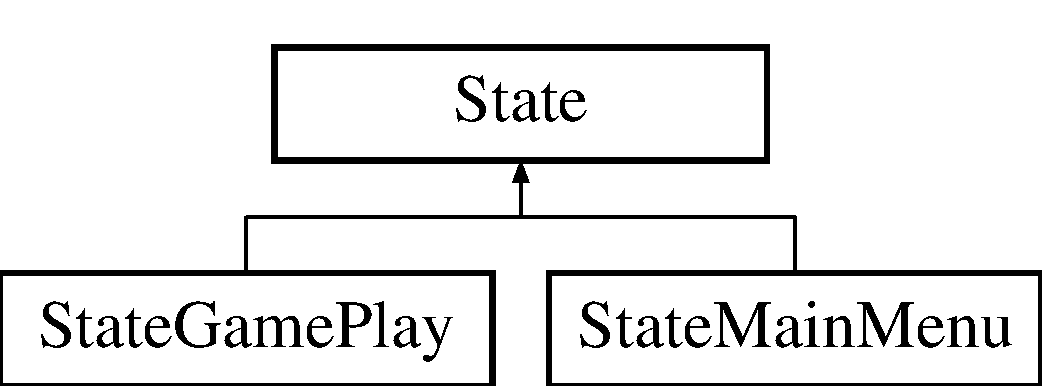
\includegraphics[height=2.000000cm]{class_state}
\end{center}
\end{figure}
\subsection*{Public Member Functions}
\begin{DoxyCompactItemize}
\item 
\hyperlink{class_state_a4da3d6c4c175efa74f87a1d413a4486b}{State} (const \hyperlink{_state_8hpp_a905494cc15ee9757a813dbfe4b1072fe}{State\-I\-D} state\-I\-D)
\begin{DoxyCompactList}\small\item\em \hyperlink{class_state}{State} ctor. \end{DoxyCompactList}\item 
virtual \hyperlink{class_state_afab438d92b90dc18d194dbd9c9c8bab3}{$\sim$\-State} ()
\begin{DoxyCompactList}\small\item\em $\sim$\-State virtual dtor. \end{DoxyCompactList}\item 
\hyperlink{_state_8hpp_a905494cc15ee9757a813dbfe4b1072fe}{State\-I\-D} \hyperlink{class_state_ab7022716d4d0c7aec82dbdd90e1e039e}{Get\-I\-D} () const 
\begin{DoxyCompactList}\small\item\em Get\-I\-D getter for the state id. \end{DoxyCompactList}\item 
virtual void \hyperlink{class_state_a43d4ca30d927c023316c058b700c0716}{Update} ()=0
\begin{DoxyCompactList}\small\item\em Update pure virtual call to update the child class. \end{DoxyCompactList}\item 
virtual void \hyperlink{class_state_a8b0cdb0e7450a9bb3580a33dfbe4d981}{Draw} ()=0
\begin{DoxyCompactList}\small\item\em Draw pure virtual call to draw the child class. \end{DoxyCompactList}\item 
virtual void \hyperlink{class_state_a8c96aac63e62b9b6bb491cae071d08f2}{Load\-From\-X\-M\-L} (const string \&file)=0
\begin{DoxyCompactList}\small\item\em Load\-From\-X\-M\-L pure virtual call to load the child classes data from an xml file. \end{DoxyCompactList}\item 
virtual void \hyperlink{class_state_aac4126b251b0c55d5c934982310c80ae}{Process\-Event} (const sf\-::\-Event \&event)=0
\begin{DoxyCompactList}\small\item\em Process\-Event pure virtual call, is where operating system events can be processed. \end{DoxyCompactList}\end{DoxyCompactItemize}
\subsection*{Protected Attributes}
\begin{DoxyCompactItemize}
\item 
\hyperlink{class_game}{Game} $\ast$ \hyperlink{class_state_a418f507cf3deef8f3653b8209a9f7b85}{mp\-Game}
\item 
\hyperlink{class_resource_manager}{Resource\-Manager}$<$ sf\-::\-Texture $>$ \hyperlink{class_state_a4eb530bbd8c56bb10ab4e36adeb097d9}{m\-Textures}
\item 
unique\-\_\-ptr$<$ \hyperlink{class_audio_effects}{Audio\-Effects} $>$ \hyperlink{class_state_a5b54964067de86bec58088f13d5a7564}{mp\-Audio\-Effects}
\item 
unique\-\_\-ptr$<$ sf\-::\-Sprite $>$ \hyperlink{class_state_ad77d6e8727cab4ac8ac5d44eacb41eba}{mp\-Background}
\end{DoxyCompactItemize}


\subsection{Detailed Description}
The \hyperlink{class_state}{State} class is the base class for states. 

This is meant to be inherited from, to create concrete state types.

The states are for the different states the game maybe in.

There are 4 pure virtual methods, Update and Draw are for updating and drawing of all the child states.

Load\-From\-X\-M\-L is for loading the states data, which should be unique to each state.

Process\-Event is where the states can become aware of operating system messages such as keypresses.

Each state keeps track of the State\-I\-D which signifies what type of state it is. 

Definition at line 56 of file State.\-hpp.



\subsection{Constructor \& Destructor Documentation}
\hypertarget{class_state_a4da3d6c4c175efa74f87a1d413a4486b}{\index{State@{State}!State@{State}}
\index{State@{State}!State@{State}}
\subsubsection[{State}]{\setlength{\rightskip}{0pt plus 5cm}State\-::\-State (
\begin{DoxyParamCaption}
\item[{const {\bf State\-I\-D}}]{state\-I\-D}
\end{DoxyParamCaption}
)}}\label{class_state_a4da3d6c4c175efa74f87a1d413a4486b}


\hyperlink{class_state}{State} ctor. 


\begin{DoxyParams}{Parameters}
{\em state\-I\-D} & The enum to signify what type of state the child is. \\
\hline
\end{DoxyParams}


Definition at line 20 of file State.\-cpp.

\hypertarget{class_state_afab438d92b90dc18d194dbd9c9c8bab3}{\index{State@{State}!$\sim$\-State@{$\sim$\-State}}
\index{$\sim$\-State@{$\sim$\-State}!State@{State}}
\subsubsection[{$\sim$\-State}]{\setlength{\rightskip}{0pt plus 5cm}State\-::$\sim$\-State (
\begin{DoxyParamCaption}
{}
\end{DoxyParamCaption}
)\hspace{0.3cm}{\ttfamily [virtual]}}}\label{class_state_afab438d92b90dc18d194dbd9c9c8bab3}


$\sim$\-State virtual dtor. 



Definition at line 30 of file State.\-cpp.



\subsection{Member Function Documentation}
\hypertarget{class_state_a8b0cdb0e7450a9bb3580a33dfbe4d981}{\index{State@{State}!Draw@{Draw}}
\index{Draw@{Draw}!State@{State}}
\subsubsection[{Draw}]{\setlength{\rightskip}{0pt plus 5cm}virtual void State\-::\-Draw (
\begin{DoxyParamCaption}
{}
\end{DoxyParamCaption}
)\hspace{0.3cm}{\ttfamily [pure virtual]}}}\label{class_state_a8b0cdb0e7450a9bb3580a33dfbe4d981}


Draw pure virtual call to draw the child class. 



Implemented in \hyperlink{class_state_main_menu_acd8b820dddbd9bd5515b1a3cebbe6978}{State\-Main\-Menu}, and \hyperlink{class_state_game_play_a5a4710616480b177cc8164675d5295ae}{State\-Game\-Play}.

\hypertarget{class_state_ab7022716d4d0c7aec82dbdd90e1e039e}{\index{State@{State}!Get\-I\-D@{Get\-I\-D}}
\index{Get\-I\-D@{Get\-I\-D}!State@{State}}
\subsubsection[{Get\-I\-D}]{\setlength{\rightskip}{0pt plus 5cm}{\bf State\-I\-D} State\-::\-Get\-I\-D (
\begin{DoxyParamCaption}
{}
\end{DoxyParamCaption}
) const}}\label{class_state_ab7022716d4d0c7aec82dbdd90e1e039e}


Get\-I\-D getter for the state id. 

\begin{DoxyReturn}{Returns}
This states I\-D. 
\end{DoxyReturn}


Definition at line 35 of file State.\-cpp.

\hypertarget{class_state_a8c96aac63e62b9b6bb491cae071d08f2}{\index{State@{State}!Load\-From\-X\-M\-L@{Load\-From\-X\-M\-L}}
\index{Load\-From\-X\-M\-L@{Load\-From\-X\-M\-L}!State@{State}}
\subsubsection[{Load\-From\-X\-M\-L}]{\setlength{\rightskip}{0pt plus 5cm}virtual void State\-::\-Load\-From\-X\-M\-L (
\begin{DoxyParamCaption}
\item[{const string \&}]{file}
\end{DoxyParamCaption}
)\hspace{0.3cm}{\ttfamily [pure virtual]}}}\label{class_state_a8c96aac63e62b9b6bb491cae071d08f2}


Load\-From\-X\-M\-L pure virtual call to load the child classes data from an xml file. 


\begin{DoxyParams}{Parameters}
{\em file} & The file name and path to an xml file. \\
\hline
\end{DoxyParams}


Implemented in \hyperlink{class_state_main_menu_a988befa6ae7c087935581b269fb8863f}{State\-Main\-Menu}, and \hyperlink{class_state_game_play_ab959c0ecf1e0db614a89a87bacd1ead1}{State\-Game\-Play}.

\hypertarget{class_state_aac4126b251b0c55d5c934982310c80ae}{\index{State@{State}!Process\-Event@{Process\-Event}}
\index{Process\-Event@{Process\-Event}!State@{State}}
\subsubsection[{Process\-Event}]{\setlength{\rightskip}{0pt plus 5cm}virtual void State\-::\-Process\-Event (
\begin{DoxyParamCaption}
\item[{const sf\-::\-Event \&}]{event}
\end{DoxyParamCaption}
)\hspace{0.3cm}{\ttfamily [pure virtual]}}}\label{class_state_aac4126b251b0c55d5c934982310c80ae}


Process\-Event pure virtual call, is where operating system events can be processed. 


\begin{DoxyParams}{Parameters}
{\em event} & The sfml Event to be processed. \\
\hline
\end{DoxyParams}


Implemented in \hyperlink{class_state_main_menu_ac9a02be51b4faa9c7d82e10af97ef6e4}{State\-Main\-Menu}, and \hyperlink{class_state_game_play_a9123dfdcf99f92706a00740245e98d23}{State\-Game\-Play}.

\hypertarget{class_state_a43d4ca30d927c023316c058b700c0716}{\index{State@{State}!Update@{Update}}
\index{Update@{Update}!State@{State}}
\subsubsection[{Update}]{\setlength{\rightskip}{0pt plus 5cm}virtual void State\-::\-Update (
\begin{DoxyParamCaption}
{}
\end{DoxyParamCaption}
)\hspace{0.3cm}{\ttfamily [pure virtual]}}}\label{class_state_a43d4ca30d927c023316c058b700c0716}


Update pure virtual call to update the child class. 



Implemented in \hyperlink{class_state_main_menu_afa9c12c0975a2af95fdd2cf1829c56df}{State\-Main\-Menu}, and \hyperlink{class_state_game_play_a56b45e9ee196d709557dac2a3a6f2b3d}{State\-Game\-Play}.



\subsection{Member Data Documentation}
\hypertarget{class_state_a5b54964067de86bec58088f13d5a7564}{\index{State@{State}!mp\-Audio\-Effects@{mp\-Audio\-Effects}}
\index{mp\-Audio\-Effects@{mp\-Audio\-Effects}!State@{State}}
\subsubsection[{mp\-Audio\-Effects}]{\setlength{\rightskip}{0pt plus 5cm}unique\-\_\-ptr$<${\bf Audio\-Effects}$>$ State\-::mp\-Audio\-Effects\hspace{0.3cm}{\ttfamily [protected]}}}\label{class_state_a5b54964067de86bec58088f13d5a7564}


Definition at line 105 of file State.\-hpp.

\hypertarget{class_state_ad77d6e8727cab4ac8ac5d44eacb41eba}{\index{State@{State}!mp\-Background@{mp\-Background}}
\index{mp\-Background@{mp\-Background}!State@{State}}
\subsubsection[{mp\-Background}]{\setlength{\rightskip}{0pt plus 5cm}unique\-\_\-ptr$<$sf\-::\-Sprite$>$ State\-::mp\-Background\hspace{0.3cm}{\ttfamily [protected]}}}\label{class_state_ad77d6e8727cab4ac8ac5d44eacb41eba}


Definition at line 106 of file State.\-hpp.

\hypertarget{class_state_a418f507cf3deef8f3653b8209a9f7b85}{\index{State@{State}!mp\-Game@{mp\-Game}}
\index{mp\-Game@{mp\-Game}!State@{State}}
\subsubsection[{mp\-Game}]{\setlength{\rightskip}{0pt plus 5cm}{\bf Game}$\ast$ State\-::mp\-Game\hspace{0.3cm}{\ttfamily [protected]}}}\label{class_state_a418f507cf3deef8f3653b8209a9f7b85}


Definition at line 102 of file State.\-hpp.

\hypertarget{class_state_a4eb530bbd8c56bb10ab4e36adeb097d9}{\index{State@{State}!m\-Textures@{m\-Textures}}
\index{m\-Textures@{m\-Textures}!State@{State}}
\subsubsection[{m\-Textures}]{\setlength{\rightskip}{0pt plus 5cm}{\bf Resource\-Manager}$<$sf\-::\-Texture$>$ State\-::m\-Textures\hspace{0.3cm}{\ttfamily [protected]}}}\label{class_state_a4eb530bbd8c56bb10ab4e36adeb097d9}


Definition at line 104 of file State.\-hpp.



The documentation for this class was generated from the following files\-:\begin{DoxyCompactItemize}
\item 
/home/lee/\-Projects/\-Sudden\-Awakening/\-Source/\hyperlink{_state_8hpp}{State.\-hpp}\item 
/home/lee/\-Projects/\-Sudden\-Awakening/\-Source/\hyperlink{_state_8cpp}{State.\-cpp}\end{DoxyCompactItemize}

\hypertarget{class_state_game_play}{\section{State\-Game\-Play Class Reference}
\label{class_state_game_play}\index{State\-Game\-Play@{State\-Game\-Play}}
}


{\ttfamily \#include $<$State\-Game\-Play.\-hpp$>$}

Inheritance diagram for State\-Game\-Play\-:\begin{figure}[H]
\begin{center}
\leavevmode
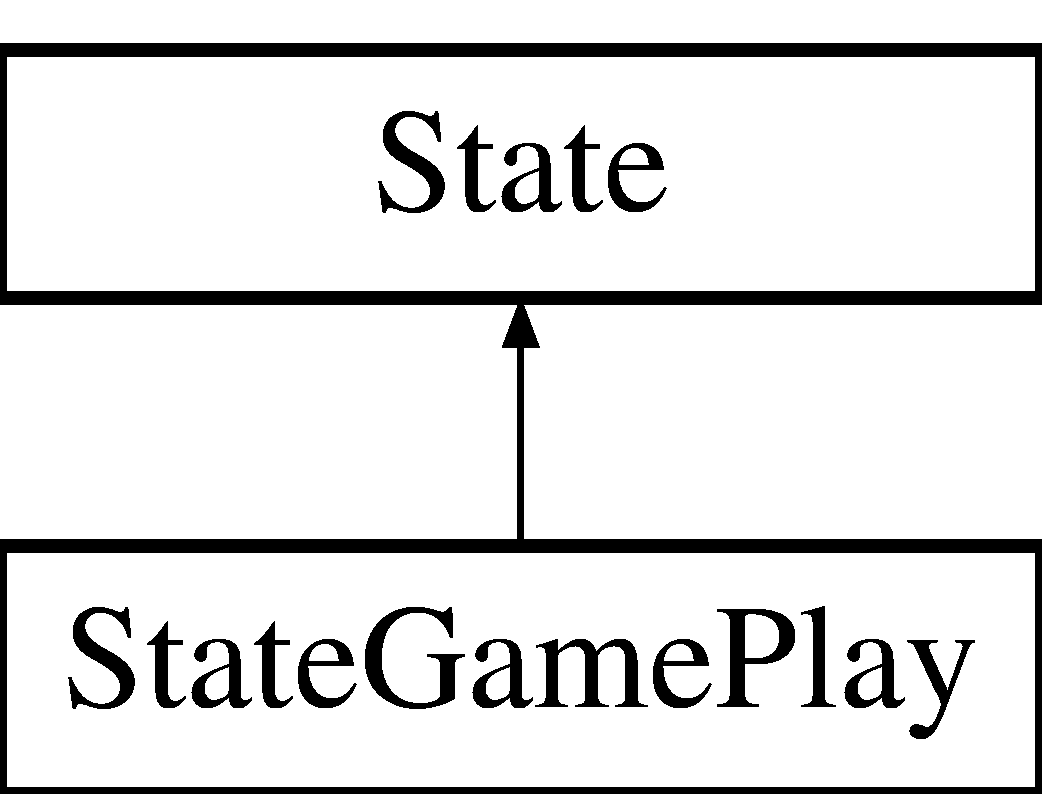
\includegraphics[height=2.000000cm]{class_state_game_play}
\end{center}
\end{figure}
\subsection*{Public Member Functions}
\begin{DoxyCompactItemize}
\item 
\hyperlink{class_state_game_play_ad7bfeabc7184e166b372e63c68c1ace9}{State\-Game\-Play} ()
\item 
virtual \hyperlink{class_state_game_play_aa4538a8a8ff81e66c0c826249d410c63}{$\sim$\-State\-Game\-Play} ()
\item 
virtual void \hyperlink{class_state_game_play_a56b45e9ee196d709557dac2a3a6f2b3d}{Update} ()
\item 
virtual void \hyperlink{class_state_game_play_a5a4710616480b177cc8164675d5295ae}{Draw} ()
\item 
virtual void \hyperlink{class_state_game_play_ab959c0ecf1e0db614a89a87bacd1ead1}{Load\-From\-X\-M\-L} (const string \&file)
\item 
virtual void \hyperlink{class_state_game_play_a9123dfdcf99f92706a00740245e98d23}{Process\-Event} (const sf\-::\-Event \&event)
\item 
\hyperlink{class_level}{Level} $\ast$ \hyperlink{class_state_game_play_a5bd072a6e7414b47fd9fcdfa34301aa6}{Get\-Level} ()
\end{DoxyCompactItemize}
\subsection*{Additional Inherited Members}


\subsection{Detailed Description}


Definition at line 10 of file State\-Game\-Play.\-hpp.



\subsection{Constructor \& Destructor Documentation}
\hypertarget{class_state_game_play_ad7bfeabc7184e166b372e63c68c1ace9}{\index{State\-Game\-Play@{State\-Game\-Play}!State\-Game\-Play@{State\-Game\-Play}}
\index{State\-Game\-Play@{State\-Game\-Play}!StateGamePlay@{State\-Game\-Play}}
\subsubsection[{State\-Game\-Play}]{\setlength{\rightskip}{0pt plus 5cm}State\-Game\-Play\-::\-State\-Game\-Play (
\begin{DoxyParamCaption}
{}
\end{DoxyParamCaption}
)}}\label{class_state_game_play_ad7bfeabc7184e166b372e63c68c1ace9}


Definition at line 9 of file State\-Game\-Play.\-cpp.

\hypertarget{class_state_game_play_aa4538a8a8ff81e66c0c826249d410c63}{\index{State\-Game\-Play@{State\-Game\-Play}!$\sim$\-State\-Game\-Play@{$\sim$\-State\-Game\-Play}}
\index{$\sim$\-State\-Game\-Play@{$\sim$\-State\-Game\-Play}!StateGamePlay@{State\-Game\-Play}}
\subsubsection[{$\sim$\-State\-Game\-Play}]{\setlength{\rightskip}{0pt plus 5cm}State\-Game\-Play\-::$\sim$\-State\-Game\-Play (
\begin{DoxyParamCaption}
{}
\end{DoxyParamCaption}
)\hspace{0.3cm}{\ttfamily [virtual]}}}\label{class_state_game_play_aa4538a8a8ff81e66c0c826249d410c63}


Definition at line 16 of file State\-Game\-Play.\-cpp.



\subsection{Member Function Documentation}
\hypertarget{class_state_game_play_a5a4710616480b177cc8164675d5295ae}{\index{State\-Game\-Play@{State\-Game\-Play}!Draw@{Draw}}
\index{Draw@{Draw}!StateGamePlay@{State\-Game\-Play}}
\subsubsection[{Draw}]{\setlength{\rightskip}{0pt plus 5cm}void State\-Game\-Play\-::\-Draw (
\begin{DoxyParamCaption}
{}
\end{DoxyParamCaption}
)\hspace{0.3cm}{\ttfamily [virtual]}}}\label{class_state_game_play_a5a4710616480b177cc8164675d5295ae}


Implements \hyperlink{class_state_a8b0cdb0e7450a9bb3580a33dfbe4d981}{State}.



Definition at line 27 of file State\-Game\-Play.\-cpp.

\hypertarget{class_state_game_play_a5bd072a6e7414b47fd9fcdfa34301aa6}{\index{State\-Game\-Play@{State\-Game\-Play}!Get\-Level@{Get\-Level}}
\index{Get\-Level@{Get\-Level}!StateGamePlay@{State\-Game\-Play}}
\subsubsection[{Get\-Level}]{\setlength{\rightskip}{0pt plus 5cm}{\bf Level}$\ast$ State\-Game\-Play\-::\-Get\-Level (
\begin{DoxyParamCaption}
{}
\end{DoxyParamCaption}
)}}\label{class_state_game_play_a5bd072a6e7414b47fd9fcdfa34301aa6}
\hypertarget{class_state_game_play_ab959c0ecf1e0db614a89a87bacd1ead1}{\index{State\-Game\-Play@{State\-Game\-Play}!Load\-From\-X\-M\-L@{Load\-From\-X\-M\-L}}
\index{Load\-From\-X\-M\-L@{Load\-From\-X\-M\-L}!StateGamePlay@{State\-Game\-Play}}
\subsubsection[{Load\-From\-X\-M\-L}]{\setlength{\rightskip}{0pt plus 5cm}void State\-Game\-Play\-::\-Load\-From\-X\-M\-L (
\begin{DoxyParamCaption}
\item[{const string \&}]{file}
\end{DoxyParamCaption}
)\hspace{0.3cm}{\ttfamily [virtual]}}}\label{class_state_game_play_ab959c0ecf1e0db614a89a87bacd1ead1}


Implements \hyperlink{class_state_a8c96aac63e62b9b6bb491cae071d08f2}{State}.



Definition at line 34 of file State\-Game\-Play.\-cpp.

\hypertarget{class_state_game_play_a9123dfdcf99f92706a00740245e98d23}{\index{State\-Game\-Play@{State\-Game\-Play}!Process\-Event@{Process\-Event}}
\index{Process\-Event@{Process\-Event}!StateGamePlay@{State\-Game\-Play}}
\subsubsection[{Process\-Event}]{\setlength{\rightskip}{0pt plus 5cm}void State\-Game\-Play\-::\-Process\-Event (
\begin{DoxyParamCaption}
\item[{const sf\-::\-Event \&}]{event}
\end{DoxyParamCaption}
)\hspace{0.3cm}{\ttfamily [virtual]}}}\label{class_state_game_play_a9123dfdcf99f92706a00740245e98d23}


Implements \hyperlink{class_state_aac4126b251b0c55d5c934982310c80ae}{State}.



Definition at line 39 of file State\-Game\-Play.\-cpp.

\hypertarget{class_state_game_play_a56b45e9ee196d709557dac2a3a6f2b3d}{\index{State\-Game\-Play@{State\-Game\-Play}!Update@{Update}}
\index{Update@{Update}!StateGamePlay@{State\-Game\-Play}}
\subsubsection[{Update}]{\setlength{\rightskip}{0pt plus 5cm}void State\-Game\-Play\-::\-Update (
\begin{DoxyParamCaption}
{}
\end{DoxyParamCaption}
)\hspace{0.3cm}{\ttfamily [virtual]}}}\label{class_state_game_play_a56b45e9ee196d709557dac2a3a6f2b3d}


Implements \hyperlink{class_state_a43d4ca30d927c023316c058b700c0716}{State}.



Definition at line 21 of file State\-Game\-Play.\-cpp.



The documentation for this class was generated from the following files\-:\begin{DoxyCompactItemize}
\item 
Source/\hyperlink{_state_game_play_8hpp}{State\-Game\-Play.\-hpp}\item 
Source/\hyperlink{_state_game_play_8cpp}{State\-Game\-Play.\-cpp}\end{DoxyCompactItemize}

\hypertarget{class_state_main_menu}{\section{State\-Main\-Menu Class Reference}
\label{class_state_main_menu}\index{State\-Main\-Menu@{State\-Main\-Menu}}
}


{\ttfamily \#include $<$State\-Main\-Menu.\-hpp$>$}

Inheritance diagram for State\-Main\-Menu\-:\begin{figure}[H]
\begin{center}
\leavevmode
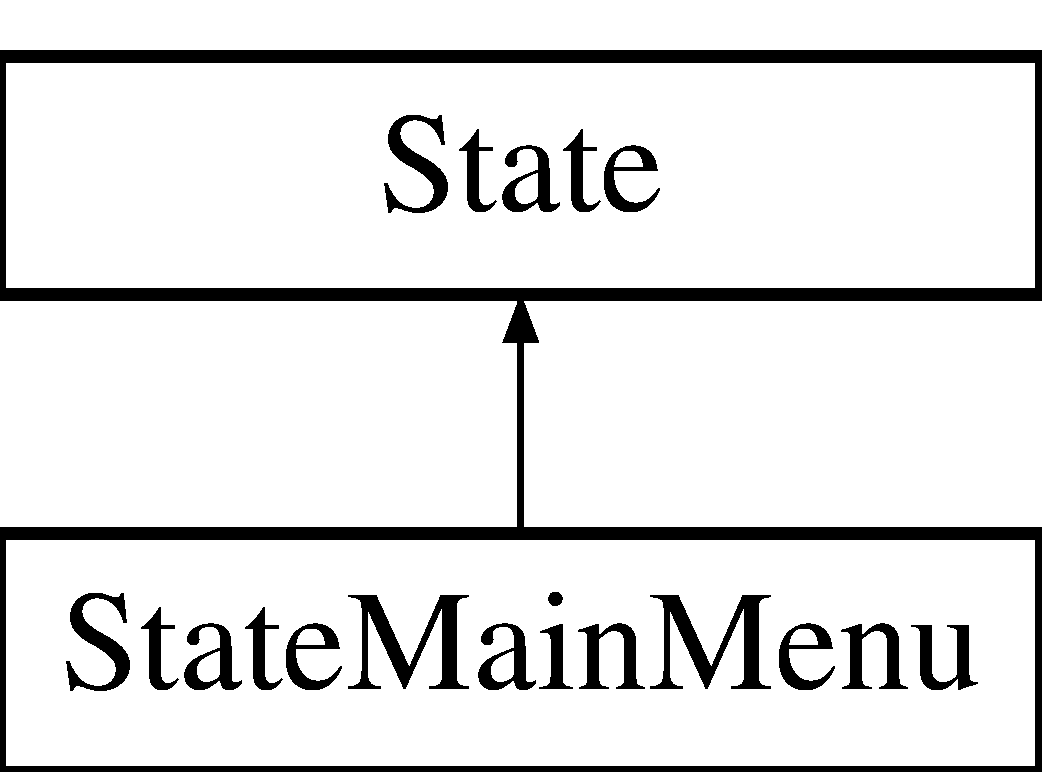
\includegraphics[height=2.000000cm]{class_state_main_menu}
\end{center}
\end{figure}
\subsection*{Public Member Functions}
\begin{DoxyCompactItemize}
\item 
\hyperlink{class_state_main_menu_af1bc1b6bfef9775a92eda9dd4c5f8d80}{State\-Main\-Menu} ()
\item 
virtual \hyperlink{class_state_main_menu_aae1ad451be64082e6e8f021d72d2050c}{$\sim$\-State\-Main\-Menu} ()
\item 
virtual void \hyperlink{class_state_main_menu_afa9c12c0975a2af95fdd2cf1829c56df}{Update} ()
\begin{DoxyCompactList}\small\item\em Update pure virtual call to update the child class. \end{DoxyCompactList}\item 
virtual void \hyperlink{class_state_main_menu_acd8b820dddbd9bd5515b1a3cebbe6978}{Draw} ()
\begin{DoxyCompactList}\small\item\em Draw pure virtual call to draw the child class. \end{DoxyCompactList}\item 
virtual void \hyperlink{class_state_main_menu_a988befa6ae7c087935581b269fb8863f}{Load\-From\-X\-M\-L} (const string \&file)
\begin{DoxyCompactList}\small\item\em Load\-From\-X\-M\-L pure virtual call to load the child classes data from an xml file. \end{DoxyCompactList}\item 
virtual void \hyperlink{class_state_main_menu_ac9a02be51b4faa9c7d82e10af97ef6e4}{Process\-Event} (const sf\-::\-Event \&event)
\begin{DoxyCompactList}\small\item\em Process\-Event pure virtual call, is where operating system events can be processed. \end{DoxyCompactList}\end{DoxyCompactItemize}
\subsection*{Additional Inherited Members}


\subsection{Detailed Description}


Definition at line 19 of file State\-Main\-Menu.\-hpp.



\subsection{Constructor \& Destructor Documentation}
\hypertarget{class_state_main_menu_af1bc1b6bfef9775a92eda9dd4c5f8d80}{\index{State\-Main\-Menu@{State\-Main\-Menu}!State\-Main\-Menu@{State\-Main\-Menu}}
\index{State\-Main\-Menu@{State\-Main\-Menu}!StateMainMenu@{State\-Main\-Menu}}
\subsubsection[{State\-Main\-Menu}]{\setlength{\rightskip}{0pt plus 5cm}State\-Main\-Menu\-::\-State\-Main\-Menu (
\begin{DoxyParamCaption}
{}
\end{DoxyParamCaption}
)}}\label{class_state_main_menu_af1bc1b6bfef9775a92eda9dd4c5f8d80}


Definition at line 21 of file State\-Main\-Menu.\-cpp.

\hypertarget{class_state_main_menu_aae1ad451be64082e6e8f021d72d2050c}{\index{State\-Main\-Menu@{State\-Main\-Menu}!$\sim$\-State\-Main\-Menu@{$\sim$\-State\-Main\-Menu}}
\index{$\sim$\-State\-Main\-Menu@{$\sim$\-State\-Main\-Menu}!StateMainMenu@{State\-Main\-Menu}}
\subsubsection[{$\sim$\-State\-Main\-Menu}]{\setlength{\rightskip}{0pt plus 5cm}State\-Main\-Menu\-::$\sim$\-State\-Main\-Menu (
\begin{DoxyParamCaption}
{}
\end{DoxyParamCaption}
)\hspace{0.3cm}{\ttfamily [virtual]}}}\label{class_state_main_menu_aae1ad451be64082e6e8f021d72d2050c}


Definition at line 39 of file State\-Main\-Menu.\-cpp.



\subsection{Member Function Documentation}
\hypertarget{class_state_main_menu_acd8b820dddbd9bd5515b1a3cebbe6978}{\index{State\-Main\-Menu@{State\-Main\-Menu}!Draw@{Draw}}
\index{Draw@{Draw}!StateMainMenu@{State\-Main\-Menu}}
\subsubsection[{Draw}]{\setlength{\rightskip}{0pt plus 5cm}void State\-Main\-Menu\-::\-Draw (
\begin{DoxyParamCaption}
{}
\end{DoxyParamCaption}
)\hspace{0.3cm}{\ttfamily [virtual]}}}\label{class_state_main_menu_acd8b820dddbd9bd5515b1a3cebbe6978}


Draw pure virtual call to draw the child class. 



Implements \hyperlink{class_state_a8b0cdb0e7450a9bb3580a33dfbe4d981}{State}.



Definition at line 86 of file State\-Main\-Menu.\-cpp.

\hypertarget{class_state_main_menu_a988befa6ae7c087935581b269fb8863f}{\index{State\-Main\-Menu@{State\-Main\-Menu}!Load\-From\-X\-M\-L@{Load\-From\-X\-M\-L}}
\index{Load\-From\-X\-M\-L@{Load\-From\-X\-M\-L}!StateMainMenu@{State\-Main\-Menu}}
\subsubsection[{Load\-From\-X\-M\-L}]{\setlength{\rightskip}{0pt plus 5cm}void State\-Main\-Menu\-::\-Load\-From\-X\-M\-L (
\begin{DoxyParamCaption}
\item[{const string \&}]{file}
\end{DoxyParamCaption}
)\hspace{0.3cm}{\ttfamily [virtual]}}}\label{class_state_main_menu_a988befa6ae7c087935581b269fb8863f}


Load\-From\-X\-M\-L pure virtual call to load the child classes data from an xml file. 


\begin{DoxyParams}{Parameters}
{\em file} & The file name and path to an xml file. \\
\hline
\end{DoxyParams}


Implements \hyperlink{class_state_a8c96aac63e62b9b6bb491cae071d08f2}{State}.



Definition at line 154 of file State\-Main\-Menu.\-cpp.

\hypertarget{class_state_main_menu_ac9a02be51b4faa9c7d82e10af97ef6e4}{\index{State\-Main\-Menu@{State\-Main\-Menu}!Process\-Event@{Process\-Event}}
\index{Process\-Event@{Process\-Event}!StateMainMenu@{State\-Main\-Menu}}
\subsubsection[{Process\-Event}]{\setlength{\rightskip}{0pt plus 5cm}void State\-Main\-Menu\-::\-Process\-Event (
\begin{DoxyParamCaption}
\item[{const sf\-::\-Event \&}]{event}
\end{DoxyParamCaption}
)\hspace{0.3cm}{\ttfamily [virtual]}}}\label{class_state_main_menu_ac9a02be51b4faa9c7d82e10af97ef6e4}


Process\-Event pure virtual call, is where operating system events can be processed. 


\begin{DoxyParams}{Parameters}
{\em event} & The sfml Event to be processed. \\
\hline
\end{DoxyParams}


Implements \hyperlink{class_state_aac4126b251b0c55d5c934982310c80ae}{State}.



Definition at line 99 of file State\-Main\-Menu.\-cpp.

\hypertarget{class_state_main_menu_afa9c12c0975a2af95fdd2cf1829c56df}{\index{State\-Main\-Menu@{State\-Main\-Menu}!Update@{Update}}
\index{Update@{Update}!StateMainMenu@{State\-Main\-Menu}}
\subsubsection[{Update}]{\setlength{\rightskip}{0pt plus 5cm}void State\-Main\-Menu\-::\-Update (
\begin{DoxyParamCaption}
{}
\end{DoxyParamCaption}
)\hspace{0.3cm}{\ttfamily [virtual]}}}\label{class_state_main_menu_afa9c12c0975a2af95fdd2cf1829c56df}


Update pure virtual call to update the child class. 



Implements \hyperlink{class_state_a43d4ca30d927c023316c058b700c0716}{State}.



Definition at line 44 of file State\-Main\-Menu.\-cpp.



The documentation for this class was generated from the following files\-:\begin{DoxyCompactItemize}
\item 
/home/chris/\-Projects/\-Sudden\-Awakening/\-Source/\hyperlink{_state_main_menu_8hpp}{State\-Main\-Menu.\-hpp}\item 
/home/chris/\-Projects/\-Sudden\-Awakening/\-Source/\hyperlink{_state_main_menu_8cpp}{State\-Main\-Menu.\-cpp}\end{DoxyCompactItemize}

\hypertarget{classtinyxml2_1_1_str_pair}{\section{tinyxml2\-:\-:Str\-Pair Class Reference}
\label{classtinyxml2_1_1_str_pair}\index{tinyxml2\-::\-Str\-Pair@{tinyxml2\-::\-Str\-Pair}}
}


{\ttfamily \#include $<$tinyxml2.\-hpp$>$}

\subsection*{Public Types}
\begin{DoxyCompactItemize}
\item 
enum \{ \\*
\hyperlink{classtinyxml2_1_1_str_pair_a0301ef962e15dd94574431f1c61266c5a4f1e01a55f8efe4ca72c32d454060237}{N\-E\-E\-D\-S\-\_\-\-E\-N\-T\-I\-T\-Y\-\_\-\-P\-R\-O\-C\-E\-S\-S\-I\-N\-G} = 0x01, 
\hyperlink{classtinyxml2_1_1_str_pair_a0301ef962e15dd94574431f1c61266c5a8f2045d56e70745d718672c0da91d0e0}{N\-E\-E\-D\-S\-\_\-\-N\-E\-W\-L\-I\-N\-E\-\_\-\-N\-O\-R\-M\-A\-L\-I\-Z\-A\-T\-I\-O\-N} = 0x02, 
\hyperlink{classtinyxml2_1_1_str_pair_a0301ef962e15dd94574431f1c61266c5ab17a85f396c221811fe49263bf6f843f}{C\-O\-L\-L\-A\-P\-S\-E\-\_\-\-W\-H\-I\-T\-E\-S\-P\-A\-C\-E} = 0x04, 
\hyperlink{classtinyxml2_1_1_str_pair_a0301ef962e15dd94574431f1c61266c5aae519eb5a639858591763aa5fc6cc953}{T\-E\-X\-T\-\_\-\-E\-L\-E\-M\-E\-N\-T} = N\-E\-E\-D\-S\-\_\-\-E\-N\-T\-I\-T\-Y\-\_\-\-P\-R\-O\-C\-E\-S\-S\-I\-N\-G $|$ N\-E\-E\-D\-S\-\_\-\-N\-E\-W\-L\-I\-N\-E\-\_\-\-N\-O\-R\-M\-A\-L\-I\-Z\-A\-T\-I\-O\-N, 
\\*
\hyperlink{classtinyxml2_1_1_str_pair_a0301ef962e15dd94574431f1c61266c5a96be48cf899bfeea0aa227f984f1fa63}{T\-E\-X\-T\-\_\-\-E\-L\-E\-M\-E\-N\-T\-\_\-\-L\-E\-A\-V\-E\-\_\-\-E\-N\-T\-I\-T\-I\-E\-S} = N\-E\-E\-D\-S\-\_\-\-N\-E\-W\-L\-I\-N\-E\-\_\-\-N\-O\-R\-M\-A\-L\-I\-Z\-A\-T\-I\-O\-N, 
\hyperlink{classtinyxml2_1_1_str_pair_a0301ef962e15dd94574431f1c61266c5aaab1cbefaa977e6f772b4e2575417aeb}{A\-T\-T\-R\-I\-B\-U\-T\-E\-\_\-\-N\-A\-M\-E} = 0, 
\hyperlink{classtinyxml2_1_1_str_pair_a0301ef962e15dd94574431f1c61266c5a6d72f9ce15f50e8bcd680edf66235dfd}{A\-T\-T\-R\-I\-B\-U\-T\-E\-\_\-\-V\-A\-L\-U\-E} = N\-E\-E\-D\-S\-\_\-\-E\-N\-T\-I\-T\-Y\-\_\-\-P\-R\-O\-C\-E\-S\-S\-I\-N\-G $|$ N\-E\-E\-D\-S\-\_\-\-N\-E\-W\-L\-I\-N\-E\-\_\-\-N\-O\-R\-M\-A\-L\-I\-Z\-A\-T\-I\-O\-N, 
\hyperlink{classtinyxml2_1_1_str_pair_a0301ef962e15dd94574431f1c61266c5a2decbd2513ac14f8befa987938326399}{A\-T\-T\-R\-I\-B\-U\-T\-E\-\_\-\-V\-A\-L\-U\-E\-\_\-\-L\-E\-A\-V\-E\-\_\-\-E\-N\-T\-I\-T\-I\-E\-S} = N\-E\-E\-D\-S\-\_\-\-N\-E\-W\-L\-I\-N\-E\-\_\-\-N\-O\-R\-M\-A\-L\-I\-Z\-A\-T\-I\-O\-N, 
\\*
\hyperlink{classtinyxml2_1_1_str_pair_a0301ef962e15dd94574431f1c61266c5a067a6ec90c8beea1cf5992930d93bffa}{C\-O\-M\-M\-E\-N\-T} = N\-E\-E\-D\-S\-\_\-\-N\-E\-W\-L\-I\-N\-E\-\_\-\-N\-O\-R\-M\-A\-L\-I\-Z\-A\-T\-I\-O\-N
 \}
\end{DoxyCompactItemize}
\subsection*{Public Member Functions}
\begin{DoxyCompactItemize}
\item 
\hyperlink{classtinyxml2_1_1_str_pair_a69153963f7052de9f767d3d8c1623a70}{Str\-Pair} ()
\item 
\hyperlink{classtinyxml2_1_1_str_pair_a60bed84d2503296e1c2a73fcef1431f9}{$\sim$\-Str\-Pair} ()
\item 
void \hyperlink{classtinyxml2_1_1_str_pair_a4f05549373394266a1eecba26813c166}{Set} (char $\ast$start, char $\ast$end, int flags)
\item 
const char $\ast$ \hyperlink{classtinyxml2_1_1_str_pair_ad87e3d11330f5e689ba1e7e54c023b57}{Get\-Str} ()
\item 
bool \hyperlink{classtinyxml2_1_1_str_pair_affa1043e73a18f05d5d2faec055725a7}{Empty} () const 
\item 
void \hyperlink{classtinyxml2_1_1_str_pair_a2baf6230e18333e02ab65d0897ee3941}{Set\-Interned\-Str} (const char $\ast$str)
\item 
void \hyperlink{classtinyxml2_1_1_str_pair_a1f82ec6b5bee35ee7466d8565e43b1de}{Set\-Str} (const char $\ast$str, int flags=0)
\item 
char $\ast$ \hyperlink{classtinyxml2_1_1_str_pair_ad90521f188e9606a8fbafe5d86fb2246}{Parse\-Text} (char $\ast$in, const char $\ast$end\-Tag, int str\-Flags)
\item 
char $\ast$ \hyperlink{classtinyxml2_1_1_str_pair_aa6d8998efceba41d87ec2300c70a6085}{Parse\-Name} (char $\ast$in)
\end{DoxyCompactItemize}


\subsection{Detailed Description}


Definition at line 140 of file tinyxml2.\-hpp.



\subsection{Member Enumeration Documentation}
\hypertarget{classtinyxml2_1_1_str_pair_a0301ef962e15dd94574431f1c61266c5}{\subsubsection[{anonymous enum}]{\setlength{\rightskip}{0pt plus 5cm}anonymous enum}}\label{classtinyxml2_1_1_str_pair_a0301ef962e15dd94574431f1c61266c5}
\begin{Desc}
\item[Enumerator]\par
\begin{description}
\index{N\-E\-E\-D\-S\-\_\-\-E\-N\-T\-I\-T\-Y\-\_\-\-P\-R\-O\-C\-E\-S\-S\-I\-N\-G@{N\-E\-E\-D\-S\-\_\-\-E\-N\-T\-I\-T\-Y\-\_\-\-P\-R\-O\-C\-E\-S\-S\-I\-N\-G}!tinyxml2\-::\-Str\-Pair@{tinyxml2\-::\-Str\-Pair}}\index{tinyxml2\-::\-Str\-Pair@{tinyxml2\-::\-Str\-Pair}!N\-E\-E\-D\-S\-\_\-\-E\-N\-T\-I\-T\-Y\-\_\-\-P\-R\-O\-C\-E\-S\-S\-I\-N\-G@{N\-E\-E\-D\-S\-\_\-\-E\-N\-T\-I\-T\-Y\-\_\-\-P\-R\-O\-C\-E\-S\-S\-I\-N\-G}}\item[{\em 
\hypertarget{classtinyxml2_1_1_str_pair_a0301ef962e15dd94574431f1c61266c5a4f1e01a55f8efe4ca72c32d454060237}{N\-E\-E\-D\-S\-\_\-\-E\-N\-T\-I\-T\-Y\-\_\-\-P\-R\-O\-C\-E\-S\-S\-I\-N\-G}\label{classtinyxml2_1_1_str_pair_a0301ef962e15dd94574431f1c61266c5a4f1e01a55f8efe4ca72c32d454060237}
}]\index{N\-E\-E\-D\-S\-\_\-\-N\-E\-W\-L\-I\-N\-E\-\_\-\-N\-O\-R\-M\-A\-L\-I\-Z\-A\-T\-I\-O\-N@{N\-E\-E\-D\-S\-\_\-\-N\-E\-W\-L\-I\-N\-E\-\_\-\-N\-O\-R\-M\-A\-L\-I\-Z\-A\-T\-I\-O\-N}!tinyxml2\-::\-Str\-Pair@{tinyxml2\-::\-Str\-Pair}}\index{tinyxml2\-::\-Str\-Pair@{tinyxml2\-::\-Str\-Pair}!N\-E\-E\-D\-S\-\_\-\-N\-E\-W\-L\-I\-N\-E\-\_\-\-N\-O\-R\-M\-A\-L\-I\-Z\-A\-T\-I\-O\-N@{N\-E\-E\-D\-S\-\_\-\-N\-E\-W\-L\-I\-N\-E\-\_\-\-N\-O\-R\-M\-A\-L\-I\-Z\-A\-T\-I\-O\-N}}\item[{\em 
\hypertarget{classtinyxml2_1_1_str_pair_a0301ef962e15dd94574431f1c61266c5a8f2045d56e70745d718672c0da91d0e0}{N\-E\-E\-D\-S\-\_\-\-N\-E\-W\-L\-I\-N\-E\-\_\-\-N\-O\-R\-M\-A\-L\-I\-Z\-A\-T\-I\-O\-N}\label{classtinyxml2_1_1_str_pair_a0301ef962e15dd94574431f1c61266c5a8f2045d56e70745d718672c0da91d0e0}
}]\index{C\-O\-L\-L\-A\-P\-S\-E\-\_\-\-W\-H\-I\-T\-E\-S\-P\-A\-C\-E@{C\-O\-L\-L\-A\-P\-S\-E\-\_\-\-W\-H\-I\-T\-E\-S\-P\-A\-C\-E}!tinyxml2\-::\-Str\-Pair@{tinyxml2\-::\-Str\-Pair}}\index{tinyxml2\-::\-Str\-Pair@{tinyxml2\-::\-Str\-Pair}!C\-O\-L\-L\-A\-P\-S\-E\-\_\-\-W\-H\-I\-T\-E\-S\-P\-A\-C\-E@{C\-O\-L\-L\-A\-P\-S\-E\-\_\-\-W\-H\-I\-T\-E\-S\-P\-A\-C\-E}}\item[{\em 
\hypertarget{classtinyxml2_1_1_str_pair_a0301ef962e15dd94574431f1c61266c5ab17a85f396c221811fe49263bf6f843f}{C\-O\-L\-L\-A\-P\-S\-E\-\_\-\-W\-H\-I\-T\-E\-S\-P\-A\-C\-E}\label{classtinyxml2_1_1_str_pair_a0301ef962e15dd94574431f1c61266c5ab17a85f396c221811fe49263bf6f843f}
}]\index{T\-E\-X\-T\-\_\-\-E\-L\-E\-M\-E\-N\-T@{T\-E\-X\-T\-\_\-\-E\-L\-E\-M\-E\-N\-T}!tinyxml2\-::\-Str\-Pair@{tinyxml2\-::\-Str\-Pair}}\index{tinyxml2\-::\-Str\-Pair@{tinyxml2\-::\-Str\-Pair}!T\-E\-X\-T\-\_\-\-E\-L\-E\-M\-E\-N\-T@{T\-E\-X\-T\-\_\-\-E\-L\-E\-M\-E\-N\-T}}\item[{\em 
\hypertarget{classtinyxml2_1_1_str_pair_a0301ef962e15dd94574431f1c61266c5aae519eb5a639858591763aa5fc6cc953}{T\-E\-X\-T\-\_\-\-E\-L\-E\-M\-E\-N\-T}\label{classtinyxml2_1_1_str_pair_a0301ef962e15dd94574431f1c61266c5aae519eb5a639858591763aa5fc6cc953}
}]\index{T\-E\-X\-T\-\_\-\-E\-L\-E\-M\-E\-N\-T\-\_\-\-L\-E\-A\-V\-E\-\_\-\-E\-N\-T\-I\-T\-I\-E\-S@{T\-E\-X\-T\-\_\-\-E\-L\-E\-M\-E\-N\-T\-\_\-\-L\-E\-A\-V\-E\-\_\-\-E\-N\-T\-I\-T\-I\-E\-S}!tinyxml2\-::\-Str\-Pair@{tinyxml2\-::\-Str\-Pair}}\index{tinyxml2\-::\-Str\-Pair@{tinyxml2\-::\-Str\-Pair}!T\-E\-X\-T\-\_\-\-E\-L\-E\-M\-E\-N\-T\-\_\-\-L\-E\-A\-V\-E\-\_\-\-E\-N\-T\-I\-T\-I\-E\-S@{T\-E\-X\-T\-\_\-\-E\-L\-E\-M\-E\-N\-T\-\_\-\-L\-E\-A\-V\-E\-\_\-\-E\-N\-T\-I\-T\-I\-E\-S}}\item[{\em 
\hypertarget{classtinyxml2_1_1_str_pair_a0301ef962e15dd94574431f1c61266c5a96be48cf899bfeea0aa227f984f1fa63}{T\-E\-X\-T\-\_\-\-E\-L\-E\-M\-E\-N\-T\-\_\-\-L\-E\-A\-V\-E\-\_\-\-E\-N\-T\-I\-T\-I\-E\-S}\label{classtinyxml2_1_1_str_pair_a0301ef962e15dd94574431f1c61266c5a96be48cf899bfeea0aa227f984f1fa63}
}]\index{A\-T\-T\-R\-I\-B\-U\-T\-E\-\_\-\-N\-A\-M\-E@{A\-T\-T\-R\-I\-B\-U\-T\-E\-\_\-\-N\-A\-M\-E}!tinyxml2\-::\-Str\-Pair@{tinyxml2\-::\-Str\-Pair}}\index{tinyxml2\-::\-Str\-Pair@{tinyxml2\-::\-Str\-Pair}!A\-T\-T\-R\-I\-B\-U\-T\-E\-\_\-\-N\-A\-M\-E@{A\-T\-T\-R\-I\-B\-U\-T\-E\-\_\-\-N\-A\-M\-E}}\item[{\em 
\hypertarget{classtinyxml2_1_1_str_pair_a0301ef962e15dd94574431f1c61266c5aaab1cbefaa977e6f772b4e2575417aeb}{A\-T\-T\-R\-I\-B\-U\-T\-E\-\_\-\-N\-A\-M\-E}\label{classtinyxml2_1_1_str_pair_a0301ef962e15dd94574431f1c61266c5aaab1cbefaa977e6f772b4e2575417aeb}
}]\index{A\-T\-T\-R\-I\-B\-U\-T\-E\-\_\-\-V\-A\-L\-U\-E@{A\-T\-T\-R\-I\-B\-U\-T\-E\-\_\-\-V\-A\-L\-U\-E}!tinyxml2\-::\-Str\-Pair@{tinyxml2\-::\-Str\-Pair}}\index{tinyxml2\-::\-Str\-Pair@{tinyxml2\-::\-Str\-Pair}!A\-T\-T\-R\-I\-B\-U\-T\-E\-\_\-\-V\-A\-L\-U\-E@{A\-T\-T\-R\-I\-B\-U\-T\-E\-\_\-\-V\-A\-L\-U\-E}}\item[{\em 
\hypertarget{classtinyxml2_1_1_str_pair_a0301ef962e15dd94574431f1c61266c5a6d72f9ce15f50e8bcd680edf66235dfd}{A\-T\-T\-R\-I\-B\-U\-T\-E\-\_\-\-V\-A\-L\-U\-E}\label{classtinyxml2_1_1_str_pair_a0301ef962e15dd94574431f1c61266c5a6d72f9ce15f50e8bcd680edf66235dfd}
}]\index{A\-T\-T\-R\-I\-B\-U\-T\-E\-\_\-\-V\-A\-L\-U\-E\-\_\-\-L\-E\-A\-V\-E\-\_\-\-E\-N\-T\-I\-T\-I\-E\-S@{A\-T\-T\-R\-I\-B\-U\-T\-E\-\_\-\-V\-A\-L\-U\-E\-\_\-\-L\-E\-A\-V\-E\-\_\-\-E\-N\-T\-I\-T\-I\-E\-S}!tinyxml2\-::\-Str\-Pair@{tinyxml2\-::\-Str\-Pair}}\index{tinyxml2\-::\-Str\-Pair@{tinyxml2\-::\-Str\-Pair}!A\-T\-T\-R\-I\-B\-U\-T\-E\-\_\-\-V\-A\-L\-U\-E\-\_\-\-L\-E\-A\-V\-E\-\_\-\-E\-N\-T\-I\-T\-I\-E\-S@{A\-T\-T\-R\-I\-B\-U\-T\-E\-\_\-\-V\-A\-L\-U\-E\-\_\-\-L\-E\-A\-V\-E\-\_\-\-E\-N\-T\-I\-T\-I\-E\-S}}\item[{\em 
\hypertarget{classtinyxml2_1_1_str_pair_a0301ef962e15dd94574431f1c61266c5a2decbd2513ac14f8befa987938326399}{A\-T\-T\-R\-I\-B\-U\-T\-E\-\_\-\-V\-A\-L\-U\-E\-\_\-\-L\-E\-A\-V\-E\-\_\-\-E\-N\-T\-I\-T\-I\-E\-S}\label{classtinyxml2_1_1_str_pair_a0301ef962e15dd94574431f1c61266c5a2decbd2513ac14f8befa987938326399}
}]\index{C\-O\-M\-M\-E\-N\-T@{C\-O\-M\-M\-E\-N\-T}!tinyxml2\-::\-Str\-Pair@{tinyxml2\-::\-Str\-Pair}}\index{tinyxml2\-::\-Str\-Pair@{tinyxml2\-::\-Str\-Pair}!C\-O\-M\-M\-E\-N\-T@{C\-O\-M\-M\-E\-N\-T}}\item[{\em 
\hypertarget{classtinyxml2_1_1_str_pair_a0301ef962e15dd94574431f1c61266c5a067a6ec90c8beea1cf5992930d93bffa}{C\-O\-M\-M\-E\-N\-T}\label{classtinyxml2_1_1_str_pair_a0301ef962e15dd94574431f1c61266c5a067a6ec90c8beea1cf5992930d93bffa}
}]\end{description}
\end{Desc}


Definition at line 143 of file tinyxml2.\-hpp.



\subsection{Constructor \& Destructor Documentation}
\hypertarget{classtinyxml2_1_1_str_pair_a69153963f7052de9f767d3d8c1623a70}{\index{tinyxml2\-::\-Str\-Pair@{tinyxml2\-::\-Str\-Pair}!Str\-Pair@{Str\-Pair}}
\index{Str\-Pair@{Str\-Pair}!tinyxml2::StrPair@{tinyxml2\-::\-Str\-Pair}}
\subsubsection[{Str\-Pair}]{\setlength{\rightskip}{0pt plus 5cm}tinyxml2\-::\-Str\-Pair\-::\-Str\-Pair (
\begin{DoxyParamCaption}
{}
\end{DoxyParamCaption}
)\hspace{0.3cm}{\ttfamily [inline]}}}\label{classtinyxml2_1_1_str_pair_a69153963f7052de9f767d3d8c1623a70}


Definition at line 156 of file tinyxml2.\-hpp.

\hypertarget{classtinyxml2_1_1_str_pair_a60bed84d2503296e1c2a73fcef1431f9}{\index{tinyxml2\-::\-Str\-Pair@{tinyxml2\-::\-Str\-Pair}!$\sim$\-Str\-Pair@{$\sim$\-Str\-Pair}}
\index{$\sim$\-Str\-Pair@{$\sim$\-Str\-Pair}!tinyxml2::StrPair@{tinyxml2\-::\-Str\-Pair}}
\subsubsection[{$\sim$\-Str\-Pair}]{\setlength{\rightskip}{0pt plus 5cm}tinyxml2\-::\-Str\-Pair\-::$\sim$\-Str\-Pair (
\begin{DoxyParamCaption}
{}
\end{DoxyParamCaption}
)}}\label{classtinyxml2_1_1_str_pair_a60bed84d2503296e1c2a73fcef1431f9}


Definition at line 83 of file tinyxml2.\-cpp.



\subsection{Member Function Documentation}
\hypertarget{classtinyxml2_1_1_str_pair_affa1043e73a18f05d5d2faec055725a7}{\index{tinyxml2\-::\-Str\-Pair@{tinyxml2\-::\-Str\-Pair}!Empty@{Empty}}
\index{Empty@{Empty}!tinyxml2::StrPair@{tinyxml2\-::\-Str\-Pair}}
\subsubsection[{Empty}]{\setlength{\rightskip}{0pt plus 5cm}bool tinyxml2\-::\-Str\-Pair\-::\-Empty (
\begin{DoxyParamCaption}
{}
\end{DoxyParamCaption}
) const\hspace{0.3cm}{\ttfamily [inline]}}}\label{classtinyxml2_1_1_str_pair_affa1043e73a18f05d5d2faec055725a7}


Definition at line 168 of file tinyxml2.\-hpp.

\hypertarget{classtinyxml2_1_1_str_pair_ad87e3d11330f5e689ba1e7e54c023b57}{\index{tinyxml2\-::\-Str\-Pair@{tinyxml2\-::\-Str\-Pair}!Get\-Str@{Get\-Str}}
\index{Get\-Str@{Get\-Str}!tinyxml2::StrPair@{tinyxml2\-::\-Str\-Pair}}
\subsubsection[{Get\-Str}]{\setlength{\rightskip}{0pt plus 5cm}const char $\ast$ tinyxml2\-::\-Str\-Pair\-::\-Get\-Str (
\begin{DoxyParamCaption}
{}
\end{DoxyParamCaption}
)}}\label{classtinyxml2_1_1_str_pair_ad87e3d11330f5e689ba1e7e54c023b57}


Definition at line 178 of file tinyxml2.\-cpp.

\hypertarget{classtinyxml2_1_1_str_pair_aa6d8998efceba41d87ec2300c70a6085}{\index{tinyxml2\-::\-Str\-Pair@{tinyxml2\-::\-Str\-Pair}!Parse\-Name@{Parse\-Name}}
\index{Parse\-Name@{Parse\-Name}!tinyxml2::StrPair@{tinyxml2\-::\-Str\-Pair}}
\subsubsection[{Parse\-Name}]{\setlength{\rightskip}{0pt plus 5cm}char $\ast$ tinyxml2\-::\-Str\-Pair\-::\-Parse\-Name (
\begin{DoxyParamCaption}
\item[{char $\ast$}]{in}
\end{DoxyParamCaption}
)}}\label{classtinyxml2_1_1_str_pair_aa6d8998efceba41d87ec2300c70a6085}


Definition at line 131 of file tinyxml2.\-cpp.

\hypertarget{classtinyxml2_1_1_str_pair_ad90521f188e9606a8fbafe5d86fb2246}{\index{tinyxml2\-::\-Str\-Pair@{tinyxml2\-::\-Str\-Pair}!Parse\-Text@{Parse\-Text}}
\index{Parse\-Text@{Parse\-Text}!tinyxml2::StrPair@{tinyxml2\-::\-Str\-Pair}}
\subsubsection[{Parse\-Text}]{\setlength{\rightskip}{0pt plus 5cm}char $\ast$ tinyxml2\-::\-Str\-Pair\-::\-Parse\-Text (
\begin{DoxyParamCaption}
\item[{char $\ast$}]{in, }
\item[{const char $\ast$}]{end\-Tag, }
\item[{int}]{str\-Flags}
\end{DoxyParamCaption}
)}}\label{classtinyxml2_1_1_str_pair_ad90521f188e9606a8fbafe5d86fb2246}


Definition at line 111 of file tinyxml2.\-cpp.

\hypertarget{classtinyxml2_1_1_str_pair_a4f05549373394266a1eecba26813c166}{\index{tinyxml2\-::\-Str\-Pair@{tinyxml2\-::\-Str\-Pair}!Set@{Set}}
\index{Set@{Set}!tinyxml2::StrPair@{tinyxml2\-::\-Str\-Pair}}
\subsubsection[{Set}]{\setlength{\rightskip}{0pt plus 5cm}void tinyxml2\-::\-Str\-Pair\-::\-Set (
\begin{DoxyParamCaption}
\item[{char $\ast$}]{start, }
\item[{char $\ast$}]{end, }
\item[{int}]{flags}
\end{DoxyParamCaption}
)\hspace{0.3cm}{\ttfamily [inline]}}}\label{classtinyxml2_1_1_str_pair_a4f05549373394266a1eecba26813c166}


Definition at line 159 of file tinyxml2.\-hpp.

\hypertarget{classtinyxml2_1_1_str_pair_a2baf6230e18333e02ab65d0897ee3941}{\index{tinyxml2\-::\-Str\-Pair@{tinyxml2\-::\-Str\-Pair}!Set\-Interned\-Str@{Set\-Interned\-Str}}
\index{Set\-Interned\-Str@{Set\-Interned\-Str}!tinyxml2::StrPair@{tinyxml2\-::\-Str\-Pair}}
\subsubsection[{Set\-Interned\-Str}]{\setlength{\rightskip}{0pt plus 5cm}void tinyxml2\-::\-Str\-Pair\-::\-Set\-Interned\-Str (
\begin{DoxyParamCaption}
\item[{const char $\ast$}]{str}
\end{DoxyParamCaption}
)\hspace{0.3cm}{\ttfamily [inline]}}}\label{classtinyxml2_1_1_str_pair_a2baf6230e18333e02ab65d0897ee3941}


Definition at line 172 of file tinyxml2.\-hpp.

\hypertarget{classtinyxml2_1_1_str_pair_a1f82ec6b5bee35ee7466d8565e43b1de}{\index{tinyxml2\-::\-Str\-Pair@{tinyxml2\-::\-Str\-Pair}!Set\-Str@{Set\-Str}}
\index{Set\-Str@{Set\-Str}!tinyxml2::StrPair@{tinyxml2\-::\-Str\-Pair}}
\subsubsection[{Set\-Str}]{\setlength{\rightskip}{0pt plus 5cm}void tinyxml2\-::\-Str\-Pair\-::\-Set\-Str (
\begin{DoxyParamCaption}
\item[{const char $\ast$}]{str, }
\item[{int}]{flags = {\ttfamily 0}}
\end{DoxyParamCaption}
)}}\label{classtinyxml2_1_1_str_pair_a1f82ec6b5bee35ee7466d8565e43b1de}


Definition at line 100 of file tinyxml2.\-cpp.



The documentation for this class was generated from the following files\-:\begin{DoxyCompactItemize}
\item 
/home/lee/\-Projects/\-Sudden\-Awakening/\-Source/\hyperlink{tinyxml2_8hpp}{tinyxml2.\-hpp}\item 
/home/lee/\-Projects/\-Sudden\-Awakening/\-Source/\hyperlink{tinyxml2_8cpp}{tinyxml2.\-cpp}\end{DoxyCompactItemize}

\hypertarget{class_tile_map}{\section{Tile\-Map Class Reference}
\label{class_tile_map}\index{Tile\-Map@{Tile\-Map}}
}


The \hyperlink{class_tile_map}{Tile\-Map} class presents the a map loaded from xml files from Tiled map editor.  




{\ttfamily \#include $<$Tile\-Map.\-hpp$>$}

\subsection*{Public Member Functions}
\begin{DoxyCompactItemize}
\item 
\hyperlink{class_tile_map_a4914f83099a0cd9b71b0ab9a665956c5}{Tile\-Map} (const std\-::string \&file)
\begin{DoxyCompactList}\small\item\em \hyperlink{class_tile_map}{Tile\-Map} ctor, attempts to load the map file, throws exception if fails. \end{DoxyCompactList}\item 
virtual \hyperlink{class_tile_map_a3448728e45d6a43fff3a02d4c6d72e9d}{$\sim$\-Tile\-Map} ()
\begin{DoxyCompactList}\small\item\em $\sim$\-Tile\-Map virtual dtor. \end{DoxyCompactList}\item 
virtual void \hyperlink{class_tile_map_a03106c4fd480ab81782778a28af5484f}{Update} ()
\begin{DoxyCompactList}\small\item\em Update currently empty. Maybe something added in future. \end{DoxyCompactList}\item 
virtual void \hyperlink{class_tile_map_adc7449af6dab5033f9af54b85f2dd8b1}{Draw} (sf\-::\-Render\-Window $\ast$p\-Window) const 
\begin{DoxyCompactList}\small\item\em Draw will use sfml2 to draw the entire map with layers and transperancey. \end{DoxyCompactList}\item 
virtual bool \hyperlink{class_tile_map_abf04fac57f31135e607b0cd23bb4de1c}{Is\-Valid\-Position} (sf\-::\-Sprite $\ast$p\-Sprite) const 
\begin{DoxyCompactList}\small\item\em Is\-Valid\-Position is a check for collision. This is how collisions with the map work. \end{DoxyCompactList}\item 
virtual sf\-::\-Vector2f \hyperlink{class_tile_map_a31c15d30a5d05e3667bd37d5e46c5b56}{Get\-Spawn\-Position} () const 
\begin{DoxyCompactList}\small\item\em Get\-Spawn\-Position getter for the spawn location. \end{DoxyCompactList}\item 
virtual const \hyperlink{class_tile_map_layer}{Tile\-Map\-Layer} $\ast$ \hyperlink{class_tile_map_a8b501e63e2e7040a41b65d489a77dfaf}{Get\-Data\-Layer} () const 
\begin{DoxyCompactList}\small\item\em Get\-Data\-Layer getter for the data layer which holds the data for collisions, spawns, ect.. \end{DoxyCompactList}\end{DoxyCompactItemize}
\subsection*{Protected Member Functions}
\begin{DoxyCompactItemize}
\item 
void \hyperlink{class_tile_map_a04a757f8848ecfb120324b1225b5622c}{Load\-From\-File} ()
\begin{DoxyCompactList}\small\item\em Load\-From\-File private method for loading the tiled map from xml, can't be called outside this classes ctor. \end{DoxyCompactList}\item 
const \hyperlink{class_tile_map_set}{Tile\-Map\-Set} $\ast$ \hyperlink{class_tile_map_a103bc4ec51b473b430bb859b1d5a215e}{Get\-Tile\-Map\-Set\-From\-Gid} (const unsigned int gid) const 
\begin{DoxyCompactList}\small\item\em Get\-Tile\-Map\-Set\-From\-Gid getter for the tile map set which the gid is in. The gid represents a tile on the map. \end{DoxyCompactList}\end{DoxyCompactItemize}
\subsection*{Protected Attributes}
\begin{DoxyCompactItemize}
\item 
string \hyperlink{class_tile_map_a16522fed3a3c05fd048d4627918dac4e}{m\-File}
\item 
float \hyperlink{class_tile_map_a6067e70fab16c65ecbb49ac3a939c2a1}{m\-File\-Version}
\item 
string \hyperlink{class_tile_map_a57c00e3034715bdd4feeb0ea6170829f}{m\-Orientation}
\item 
unsigned int \hyperlink{class_tile_map_aaee5f34ef457d19fa32768301ac81fc2}{m\-Tile\-Width\-Count}
\item 
unsigned int \hyperlink{class_tile_map_a2d6863a88f0ce522376c1d90c448a385}{m\-Tile\-Height\-Count}
\item 
unsigned int \hyperlink{class_tile_map_a98fe1a15d2a9fae5ecd3290fc9700661}{m\-Tile\-Width\-Size}
\item 
unsigned int \hyperlink{class_tile_map_a74b8c66dd13864f60cea068a8872499d}{m\-Tile\-Height\-Size}
\item 
\hyperlink{class_tile_map_layer}{Tile\-Map\-Layer} $\ast$ \hyperlink{class_tile_map_a8a388c1792d2170c8c5b27098f4ef439}{mp\-Data\-Layer}
\item 
vector$<$ unique\-\_\-ptr$<$ \hyperlink{class_tile_map_set}{Tile\-Map\-Set} $>$ $>$ \hyperlink{class_tile_map_ae9003055f192d71c5b5f9032852214a2}{m\-Tile\-Sets}
\item 
vector$<$ unique\-\_\-ptr\\*
$<$ \hyperlink{class_tile_map_layer}{Tile\-Map\-Layer} $>$ $>$ \hyperlink{class_tile_map_a954cc80053d31eab8a7950a36793f7b6}{m\-Tile\-Map\-Layers}
\end{DoxyCompactItemize}


\subsection{Detailed Description}
The \hyperlink{class_tile_map}{Tile\-Map} class presents the a map loaded from xml files from Tiled map editor. 

This can load a Tiled map from editor, via xml files.

It must be in xml format.

The ctor will load the map and if there is an error will throw an exception.

Supports many layers, and many tile sets. 

Definition at line 39 of file Tile\-Map.\-hpp.



\subsection{Constructor \& Destructor Documentation}
\hypertarget{class_tile_map_a4914f83099a0cd9b71b0ab9a665956c5}{\index{Tile\-Map@{Tile\-Map}!Tile\-Map@{Tile\-Map}}
\index{Tile\-Map@{Tile\-Map}!TileMap@{Tile\-Map}}
\subsubsection[{Tile\-Map}]{\setlength{\rightskip}{0pt plus 5cm}Tile\-Map\-::\-Tile\-Map (
\begin{DoxyParamCaption}
\item[{const std\-::string \&}]{file}
\end{DoxyParamCaption}
)}}\label{class_tile_map_a4914f83099a0cd9b71b0ab9a665956c5}


\hyperlink{class_tile_map}{Tile\-Map} ctor, attempts to load the map file, throws exception if fails. 


\begin{DoxyParams}{Parameters}
{\em file} & The file name and path to a map xml file. \\
\hline
\end{DoxyParams}


Definition at line 14 of file Tile\-Map.\-cpp.

\hypertarget{class_tile_map_a3448728e45d6a43fff3a02d4c6d72e9d}{\index{Tile\-Map@{Tile\-Map}!$\sim$\-Tile\-Map@{$\sim$\-Tile\-Map}}
\index{$\sim$\-Tile\-Map@{$\sim$\-Tile\-Map}!TileMap@{Tile\-Map}}
\subsubsection[{$\sim$\-Tile\-Map}]{\setlength{\rightskip}{0pt plus 5cm}Tile\-Map\-::$\sim$\-Tile\-Map (
\begin{DoxyParamCaption}
{}
\end{DoxyParamCaption}
)\hspace{0.3cm}{\ttfamily [virtual]}}}\label{class_tile_map_a3448728e45d6a43fff3a02d4c6d72e9d}


$\sim$\-Tile\-Map virtual dtor. 



Definition at line 27 of file Tile\-Map.\-cpp.



\subsection{Member Function Documentation}
\hypertarget{class_tile_map_adc7449af6dab5033f9af54b85f2dd8b1}{\index{Tile\-Map@{Tile\-Map}!Draw@{Draw}}
\index{Draw@{Draw}!TileMap@{Tile\-Map}}
\subsubsection[{Draw}]{\setlength{\rightskip}{0pt plus 5cm}void Tile\-Map\-::\-Draw (
\begin{DoxyParamCaption}
\item[{sf\-::\-Render\-Window $\ast$}]{p\-Window}
\end{DoxyParamCaption}
) const\hspace{0.3cm}{\ttfamily [virtual]}}}\label{class_tile_map_adc7449af6dab5033f9af54b85f2dd8b1}


Draw will use sfml2 to draw the entire map with layers and transperancey. 


\begin{DoxyParams}{Parameters}
{\em p\-Window} & The S\-F\-M\-L2 window to draw to. \\
\hline
\end{DoxyParams}


Definition at line 331 of file Tile\-Map.\-cpp.

\hypertarget{class_tile_map_a8b501e63e2e7040a41b65d489a77dfaf}{\index{Tile\-Map@{Tile\-Map}!Get\-Data\-Layer@{Get\-Data\-Layer}}
\index{Get\-Data\-Layer@{Get\-Data\-Layer}!TileMap@{Tile\-Map}}
\subsubsection[{Get\-Data\-Layer}]{\setlength{\rightskip}{0pt plus 5cm}const {\bf Tile\-Map\-Layer} $\ast$ Tile\-Map\-::\-Get\-Data\-Layer (
\begin{DoxyParamCaption}
{}
\end{DoxyParamCaption}
) const\hspace{0.3cm}{\ttfamily [virtual]}}}\label{class_tile_map_a8b501e63e2e7040a41b65d489a77dfaf}


Get\-Data\-Layer getter for the data layer which holds the data for collisions, spawns, ect.. 

\begin{DoxyReturn}{Returns}
The map layer which is the data layer. 
\end{DoxyReturn}


Definition at line 352 of file Tile\-Map.\-cpp.

\hypertarget{class_tile_map_a31c15d30a5d05e3667bd37d5e46c5b56}{\index{Tile\-Map@{Tile\-Map}!Get\-Spawn\-Position@{Get\-Spawn\-Position}}
\index{Get\-Spawn\-Position@{Get\-Spawn\-Position}!TileMap@{Tile\-Map}}
\subsubsection[{Get\-Spawn\-Position}]{\setlength{\rightskip}{0pt plus 5cm}sf\-::\-Vector2f Tile\-Map\-::\-Get\-Spawn\-Position (
\begin{DoxyParamCaption}
{}
\end{DoxyParamCaption}
) const\hspace{0.3cm}{\ttfamily [virtual]}}}\label{class_tile_map_a31c15d30a5d05e3667bd37d5e46c5b56}


Get\-Spawn\-Position getter for the spawn location. 

\begin{DoxyReturn}{Returns}
The coordinate for spawning as top left corner. 
\end{DoxyReturn}


Definition at line 347 of file Tile\-Map.\-cpp.

\hypertarget{class_tile_map_a103bc4ec51b473b430bb859b1d5a215e}{\index{Tile\-Map@{Tile\-Map}!Get\-Tile\-Map\-Set\-From\-Gid@{Get\-Tile\-Map\-Set\-From\-Gid}}
\index{Get\-Tile\-Map\-Set\-From\-Gid@{Get\-Tile\-Map\-Set\-From\-Gid}!TileMap@{Tile\-Map}}
\subsubsection[{Get\-Tile\-Map\-Set\-From\-Gid}]{\setlength{\rightskip}{0pt plus 5cm}const {\bf Tile\-Map\-Set} $\ast$ Tile\-Map\-::\-Get\-Tile\-Map\-Set\-From\-Gid (
\begin{DoxyParamCaption}
\item[{const unsigned int}]{gid}
\end{DoxyParamCaption}
) const\hspace{0.3cm}{\ttfamily [protected]}}}\label{class_tile_map_a103bc4ec51b473b430bb859b1d5a215e}


Get\-Tile\-Map\-Set\-From\-Gid getter for the tile map set which the gid is in. The gid represents a tile on the map. 


\begin{DoxyParams}{Parameters}
{\em gid} & The tile I\-D. \\
\hline
\end{DoxyParams}
\begin{DoxyReturn}{Returns}
The map set which this id is on. 
\end{DoxyReturn}


Definition at line 357 of file Tile\-Map.\-cpp.

\hypertarget{class_tile_map_abf04fac57f31135e607b0cd23bb4de1c}{\index{Tile\-Map@{Tile\-Map}!Is\-Valid\-Position@{Is\-Valid\-Position}}
\index{Is\-Valid\-Position@{Is\-Valid\-Position}!TileMap@{Tile\-Map}}
\subsubsection[{Is\-Valid\-Position}]{\setlength{\rightskip}{0pt plus 5cm}bool Tile\-Map\-::\-Is\-Valid\-Position (
\begin{DoxyParamCaption}
\item[{sf\-::\-Sprite $\ast$}]{p\-Sprite}
\end{DoxyParamCaption}
) const\hspace{0.3cm}{\ttfamily [virtual]}}}\label{class_tile_map_abf04fac57f31135e607b0cd23bb4de1c}


Is\-Valid\-Position is a check for collision. This is how collisions with the map work. 


\begin{DoxyParams}{Parameters}
{\em p\-Sprite} & True if the position is valid, false if its colliding with something it shouldn't be. \\
\hline
\end{DoxyParams}
\begin{DoxyReturn}{Returns}

\end{DoxyReturn}


Definition at line 342 of file Tile\-Map.\-cpp.

\hypertarget{class_tile_map_a04a757f8848ecfb120324b1225b5622c}{\index{Tile\-Map@{Tile\-Map}!Load\-From\-File@{Load\-From\-File}}
\index{Load\-From\-File@{Load\-From\-File}!TileMap@{Tile\-Map}}
\subsubsection[{Load\-From\-File}]{\setlength{\rightskip}{0pt plus 5cm}void Tile\-Map\-::\-Load\-From\-File (
\begin{DoxyParamCaption}
{}
\end{DoxyParamCaption}
)\hspace{0.3cm}{\ttfamily [protected]}}}\label{class_tile_map_a04a757f8848ecfb120324b1225b5622c}


Load\-From\-File private method for loading the tiled map from xml, can't be called outside this classes ctor. 



Definition at line 32 of file Tile\-Map.\-cpp.

\hypertarget{class_tile_map_a03106c4fd480ab81782778a28af5484f}{\index{Tile\-Map@{Tile\-Map}!Update@{Update}}
\index{Update@{Update}!TileMap@{Tile\-Map}}
\subsubsection[{Update}]{\setlength{\rightskip}{0pt plus 5cm}void Tile\-Map\-::\-Update (
\begin{DoxyParamCaption}
{}
\end{DoxyParamCaption}
)\hspace{0.3cm}{\ttfamily [virtual]}}}\label{class_tile_map_a03106c4fd480ab81782778a28af5484f}


Update currently empty. Maybe something added in future. 

Such as animation for tiles. Or opening and closing doors. 

Definition at line 326 of file Tile\-Map.\-cpp.



\subsection{Member Data Documentation}
\hypertarget{class_tile_map_a16522fed3a3c05fd048d4627918dac4e}{\index{Tile\-Map@{Tile\-Map}!m\-File@{m\-File}}
\index{m\-File@{m\-File}!TileMap@{Tile\-Map}}
\subsubsection[{m\-File}]{\setlength{\rightskip}{0pt plus 5cm}string Tile\-Map\-::m\-File\hspace{0.3cm}{\ttfamily [protected]}}}\label{class_tile_map_a16522fed3a3c05fd048d4627918dac4e}


Definition at line 99 of file Tile\-Map.\-hpp.

\hypertarget{class_tile_map_a6067e70fab16c65ecbb49ac3a939c2a1}{\index{Tile\-Map@{Tile\-Map}!m\-File\-Version@{m\-File\-Version}}
\index{m\-File\-Version@{m\-File\-Version}!TileMap@{Tile\-Map}}
\subsubsection[{m\-File\-Version}]{\setlength{\rightskip}{0pt plus 5cm}float Tile\-Map\-::m\-File\-Version\hspace{0.3cm}{\ttfamily [protected]}}}\label{class_tile_map_a6067e70fab16c65ecbb49ac3a939c2a1}


Definition at line 101 of file Tile\-Map.\-hpp.

\hypertarget{class_tile_map_a57c00e3034715bdd4feeb0ea6170829f}{\index{Tile\-Map@{Tile\-Map}!m\-Orientation@{m\-Orientation}}
\index{m\-Orientation@{m\-Orientation}!TileMap@{Tile\-Map}}
\subsubsection[{m\-Orientation}]{\setlength{\rightskip}{0pt plus 5cm}string Tile\-Map\-::m\-Orientation\hspace{0.3cm}{\ttfamily [protected]}}}\label{class_tile_map_a57c00e3034715bdd4feeb0ea6170829f}


Definition at line 102 of file Tile\-Map.\-hpp.

\hypertarget{class_tile_map_a8a388c1792d2170c8c5b27098f4ef439}{\index{Tile\-Map@{Tile\-Map}!mp\-Data\-Layer@{mp\-Data\-Layer}}
\index{mp\-Data\-Layer@{mp\-Data\-Layer}!TileMap@{Tile\-Map}}
\subsubsection[{mp\-Data\-Layer}]{\setlength{\rightskip}{0pt plus 5cm}{\bf Tile\-Map\-Layer}$\ast$ Tile\-Map\-::mp\-Data\-Layer\hspace{0.3cm}{\ttfamily [protected]}}}\label{class_tile_map_a8a388c1792d2170c8c5b27098f4ef439}


Definition at line 110 of file Tile\-Map.\-hpp.

\hypertarget{class_tile_map_a2d6863a88f0ce522376c1d90c448a385}{\index{Tile\-Map@{Tile\-Map}!m\-Tile\-Height\-Count@{m\-Tile\-Height\-Count}}
\index{m\-Tile\-Height\-Count@{m\-Tile\-Height\-Count}!TileMap@{Tile\-Map}}
\subsubsection[{m\-Tile\-Height\-Count}]{\setlength{\rightskip}{0pt plus 5cm}unsigned int Tile\-Map\-::m\-Tile\-Height\-Count\hspace{0.3cm}{\ttfamily [protected]}}}\label{class_tile_map_a2d6863a88f0ce522376c1d90c448a385}


Definition at line 105 of file Tile\-Map.\-hpp.

\hypertarget{class_tile_map_a74b8c66dd13864f60cea068a8872499d}{\index{Tile\-Map@{Tile\-Map}!m\-Tile\-Height\-Size@{m\-Tile\-Height\-Size}}
\index{m\-Tile\-Height\-Size@{m\-Tile\-Height\-Size}!TileMap@{Tile\-Map}}
\subsubsection[{m\-Tile\-Height\-Size}]{\setlength{\rightskip}{0pt plus 5cm}unsigned int Tile\-Map\-::m\-Tile\-Height\-Size\hspace{0.3cm}{\ttfamily [protected]}}}\label{class_tile_map_a74b8c66dd13864f60cea068a8872499d}


Definition at line 108 of file Tile\-Map.\-hpp.

\hypertarget{class_tile_map_a954cc80053d31eab8a7950a36793f7b6}{\index{Tile\-Map@{Tile\-Map}!m\-Tile\-Map\-Layers@{m\-Tile\-Map\-Layers}}
\index{m\-Tile\-Map\-Layers@{m\-Tile\-Map\-Layers}!TileMap@{Tile\-Map}}
\subsubsection[{m\-Tile\-Map\-Layers}]{\setlength{\rightskip}{0pt plus 5cm}vector$<$ unique\-\_\-ptr$<$ {\bf Tile\-Map\-Layer} $>$ $>$ Tile\-Map\-::m\-Tile\-Map\-Layers\hspace{0.3cm}{\ttfamily [protected]}}}\label{class_tile_map_a954cc80053d31eab8a7950a36793f7b6}


Definition at line 113 of file Tile\-Map.\-hpp.

\hypertarget{class_tile_map_ae9003055f192d71c5b5f9032852214a2}{\index{Tile\-Map@{Tile\-Map}!m\-Tile\-Sets@{m\-Tile\-Sets}}
\index{m\-Tile\-Sets@{m\-Tile\-Sets}!TileMap@{Tile\-Map}}
\subsubsection[{m\-Tile\-Sets}]{\setlength{\rightskip}{0pt plus 5cm}vector$<$ unique\-\_\-ptr$<$ {\bf Tile\-Map\-Set} $>$ $>$ Tile\-Map\-::m\-Tile\-Sets\hspace{0.3cm}{\ttfamily [protected]}}}\label{class_tile_map_ae9003055f192d71c5b5f9032852214a2}


Definition at line 112 of file Tile\-Map.\-hpp.

\hypertarget{class_tile_map_aaee5f34ef457d19fa32768301ac81fc2}{\index{Tile\-Map@{Tile\-Map}!m\-Tile\-Width\-Count@{m\-Tile\-Width\-Count}}
\index{m\-Tile\-Width\-Count@{m\-Tile\-Width\-Count}!TileMap@{Tile\-Map}}
\subsubsection[{m\-Tile\-Width\-Count}]{\setlength{\rightskip}{0pt plus 5cm}unsigned int Tile\-Map\-::m\-Tile\-Width\-Count\hspace{0.3cm}{\ttfamily [protected]}}}\label{class_tile_map_aaee5f34ef457d19fa32768301ac81fc2}


Definition at line 104 of file Tile\-Map.\-hpp.

\hypertarget{class_tile_map_a98fe1a15d2a9fae5ecd3290fc9700661}{\index{Tile\-Map@{Tile\-Map}!m\-Tile\-Width\-Size@{m\-Tile\-Width\-Size}}
\index{m\-Tile\-Width\-Size@{m\-Tile\-Width\-Size}!TileMap@{Tile\-Map}}
\subsubsection[{m\-Tile\-Width\-Size}]{\setlength{\rightskip}{0pt plus 5cm}unsigned int Tile\-Map\-::m\-Tile\-Width\-Size\hspace{0.3cm}{\ttfamily [protected]}}}\label{class_tile_map_a98fe1a15d2a9fae5ecd3290fc9700661}


Definition at line 107 of file Tile\-Map.\-hpp.



The documentation for this class was generated from the following files\-:\begin{DoxyCompactItemize}
\item 
/home/lee/\-Projects/\-Sudden\-Awakening/\-Source/\hyperlink{_tile_map_8hpp}{Tile\-Map.\-hpp}\item 
/home/lee/\-Projects/\-Sudden\-Awakening/\-Source/\hyperlink{_tile_map_8cpp}{Tile\-Map.\-cpp}\end{DoxyCompactItemize}

\hypertarget{class_tile_map_layer}{\section{Tile\-Map\-Layer Class Reference}
\label{class_tile_map_layer}\index{Tile\-Map\-Layer@{Tile\-Map\-Layer}}
}


{\ttfamily \#include $<$Tile\-Map.\-hpp$>$}

\subsection*{Public Member Functions}
\begin{DoxyCompactItemize}
\item 
\hyperlink{class_tile_map_layer_ac9fba07c129ad2a52be1601f58eee773}{Tile\-Map\-Layer} (const string \&layer\-Name, unsigned int tile\-Width\-Count, unsigned int tile\-Height\-Count)
\item 
virtual \hyperlink{class_tile_map_layer_a8bee35e5252ed1c3c1ea6935003c5d10}{$\sim$\-Tile\-Map\-Layer} ()
\item 
virtual void \hyperlink{class_tile_map_layer_a1befe86a2d2bed2d410924875eca4847}{Update} ()
\item 
virtual void \hyperlink{class_tile_map_layer_ab09044152ad8bebc2afbe837858ac4ae}{Draw} (sf\-::\-Render\-Window $\ast$p\-Window) const 
\item 
virtual bool \hyperlink{class_tile_map_layer_af6140d8910838621911ee1aaefcf317e}{Is\-Colliding} (sf\-::\-Sprite $\ast$p\-Sprite) const 
\item 
virtual sf\-::\-Vector2f \hyperlink{class_tile_map_layer_a04a978cd751d8c67f483816827888c21}{Get\-Spawn\-Position} () const 
\item 
unsigned int \hyperlink{class_tile_map_layer_ace19c01d1db3ebd4d1d370a6b34a2db5}{Get\-Tile\-Width\-Count} () const 
\item 
unsigned int \hyperlink{class_tile_map_layer_a14fce828daafd9e07f855ad0bb274299}{Get\-Tile\-Height\-Count} () const 
\item 
void \hyperlink{class_tile_map_layer_add757a7c1952dc4e0b6cf67e2887b509}{Set\-Is\-Visible} (bool visible)
\item 
bool \hyperlink{class_tile_map_layer_a068d3fa1c63e2c78ec0feb41a441e63c}{Get\-Is\-Visible} () const 
\item 
void \hyperlink{class_tile_map_layer_a7a1e6fc535c544905cd5e96adbc0813a}{Add\-Entity} (unique\-\_\-ptr$<$ \hyperlink{class_map_entity}{Map\-Entity} $>$ p\-Ent)
\end{DoxyCompactItemize}
\subsection*{Protected Attributes}
\begin{DoxyCompactItemize}
\item 
string \hyperlink{class_tile_map_layer_a2d89ec99671ed9cd422c68a5db26a5e4}{m\-Layer\-Name}
\item 
unsigned int \hyperlink{class_tile_map_layer_a1f7ed47471eae14e321db6e2da4d0547}{m\-Tile\-Width\-Count}
\item 
unsigned int \hyperlink{class_tile_map_layer_ad3731c3f3e38579327eb1a6b40e74af3}{m\-Tile\-Height\-Count}
\item 
bool \hyperlink{class_tile_map_layer_a516864f25003dad7720675ef44e727c0}{m\-Is\-Visible}
\item 
vector$<$ unique\-\_\-ptr$<$ \hyperlink{class_map_entity}{Map\-Entity} $>$ $>$ \hyperlink{class_tile_map_layer_a9c9c569f4c2f5de09b5541d079f5f97a}{m\-Tile\-Entities}
\end{DoxyCompactItemize}


\subsection{Detailed Description}


Definition at line 60 of file Tile\-Map.\-hpp.



\subsection{Constructor \& Destructor Documentation}
\hypertarget{class_tile_map_layer_ac9fba07c129ad2a52be1601f58eee773}{\index{Tile\-Map\-Layer@{Tile\-Map\-Layer}!Tile\-Map\-Layer@{Tile\-Map\-Layer}}
\index{Tile\-Map\-Layer@{Tile\-Map\-Layer}!TileMapLayer@{Tile\-Map\-Layer}}
\subsubsection[{Tile\-Map\-Layer}]{\setlength{\rightskip}{0pt plus 5cm}Tile\-Map\-Layer\-::\-Tile\-Map\-Layer (
\begin{DoxyParamCaption}
\item[{const string \&}]{layer\-Name, }
\item[{unsigned int}]{tile\-Width\-Count, }
\item[{unsigned int}]{tile\-Height\-Count}
\end{DoxyParamCaption}
)}}\label{class_tile_map_layer_ac9fba07c129ad2a52be1601f58eee773}


Definition at line 373 of file Tile\-Map.\-cpp.

\hypertarget{class_tile_map_layer_a8bee35e5252ed1c3c1ea6935003c5d10}{\index{Tile\-Map\-Layer@{Tile\-Map\-Layer}!$\sim$\-Tile\-Map\-Layer@{$\sim$\-Tile\-Map\-Layer}}
\index{$\sim$\-Tile\-Map\-Layer@{$\sim$\-Tile\-Map\-Layer}!TileMapLayer@{Tile\-Map\-Layer}}
\subsubsection[{$\sim$\-Tile\-Map\-Layer}]{\setlength{\rightskip}{0pt plus 5cm}Tile\-Map\-Layer\-::$\sim$\-Tile\-Map\-Layer (
\begin{DoxyParamCaption}
{}
\end{DoxyParamCaption}
)\hspace{0.3cm}{\ttfamily [virtual]}}}\label{class_tile_map_layer_a8bee35e5252ed1c3c1ea6935003c5d10}


Definition at line 383 of file Tile\-Map.\-cpp.



\subsection{Member Function Documentation}
\hypertarget{class_tile_map_layer_a7a1e6fc535c544905cd5e96adbc0813a}{\index{Tile\-Map\-Layer@{Tile\-Map\-Layer}!Add\-Entity@{Add\-Entity}}
\index{Add\-Entity@{Add\-Entity}!TileMapLayer@{Tile\-Map\-Layer}}
\subsubsection[{Add\-Entity}]{\setlength{\rightskip}{0pt plus 5cm}void Tile\-Map\-Layer\-::\-Add\-Entity (
\begin{DoxyParamCaption}
\item[{unique\-\_\-ptr$<$ {\bf Map\-Entity} $>$}]{p\-Ent}
\end{DoxyParamCaption}
)}}\label{class_tile_map_layer_a7a1e6fc535c544905cd5e96adbc0813a}


Definition at line 447 of file Tile\-Map.\-cpp.

\hypertarget{class_tile_map_layer_ab09044152ad8bebc2afbe837858ac4ae}{\index{Tile\-Map\-Layer@{Tile\-Map\-Layer}!Draw@{Draw}}
\index{Draw@{Draw}!TileMapLayer@{Tile\-Map\-Layer}}
\subsubsection[{Draw}]{\setlength{\rightskip}{0pt plus 5cm}void Tile\-Map\-Layer\-::\-Draw (
\begin{DoxyParamCaption}
\item[{sf\-::\-Render\-Window $\ast$}]{p\-Window}
\end{DoxyParamCaption}
) const\hspace{0.3cm}{\ttfamily [virtual]}}}\label{class_tile_map_layer_ab09044152ad8bebc2afbe837858ac4ae}


Definition at line 393 of file Tile\-Map.\-cpp.

\hypertarget{class_tile_map_layer_a068d3fa1c63e2c78ec0feb41a441e63c}{\index{Tile\-Map\-Layer@{Tile\-Map\-Layer}!Get\-Is\-Visible@{Get\-Is\-Visible}}
\index{Get\-Is\-Visible@{Get\-Is\-Visible}!TileMapLayer@{Tile\-Map\-Layer}}
\subsubsection[{Get\-Is\-Visible}]{\setlength{\rightskip}{0pt plus 5cm}bool Tile\-Map\-Layer\-::\-Get\-Is\-Visible (
\begin{DoxyParamCaption}
{}
\end{DoxyParamCaption}
) const}}\label{class_tile_map_layer_a068d3fa1c63e2c78ec0feb41a441e63c}


Definition at line 442 of file Tile\-Map.\-cpp.

\hypertarget{class_tile_map_layer_a04a978cd751d8c67f483816827888c21}{\index{Tile\-Map\-Layer@{Tile\-Map\-Layer}!Get\-Spawn\-Position@{Get\-Spawn\-Position}}
\index{Get\-Spawn\-Position@{Get\-Spawn\-Position}!TileMapLayer@{Tile\-Map\-Layer}}
\subsubsection[{Get\-Spawn\-Position}]{\setlength{\rightskip}{0pt plus 5cm}sf\-::\-Vector2f Tile\-Map\-Layer\-::\-Get\-Spawn\-Position (
\begin{DoxyParamCaption}
{}
\end{DoxyParamCaption}
) const\hspace{0.3cm}{\ttfamily [virtual]}}}\label{class_tile_map_layer_a04a978cd751d8c67f483816827888c21}


Definition at line 415 of file Tile\-Map.\-cpp.

\hypertarget{class_tile_map_layer_a14fce828daafd9e07f855ad0bb274299}{\index{Tile\-Map\-Layer@{Tile\-Map\-Layer}!Get\-Tile\-Height\-Count@{Get\-Tile\-Height\-Count}}
\index{Get\-Tile\-Height\-Count@{Get\-Tile\-Height\-Count}!TileMapLayer@{Tile\-Map\-Layer}}
\subsubsection[{Get\-Tile\-Height\-Count}]{\setlength{\rightskip}{0pt plus 5cm}unsigned int Tile\-Map\-Layer\-::\-Get\-Tile\-Height\-Count (
\begin{DoxyParamCaption}
{}
\end{DoxyParamCaption}
) const}}\label{class_tile_map_layer_a14fce828daafd9e07f855ad0bb274299}


Definition at line 432 of file Tile\-Map.\-cpp.

\hypertarget{class_tile_map_layer_ace19c01d1db3ebd4d1d370a6b34a2db5}{\index{Tile\-Map\-Layer@{Tile\-Map\-Layer}!Get\-Tile\-Width\-Count@{Get\-Tile\-Width\-Count}}
\index{Get\-Tile\-Width\-Count@{Get\-Tile\-Width\-Count}!TileMapLayer@{Tile\-Map\-Layer}}
\subsubsection[{Get\-Tile\-Width\-Count}]{\setlength{\rightskip}{0pt plus 5cm}unsigned int Tile\-Map\-Layer\-::\-Get\-Tile\-Width\-Count (
\begin{DoxyParamCaption}
{}
\end{DoxyParamCaption}
) const}}\label{class_tile_map_layer_ace19c01d1db3ebd4d1d370a6b34a2db5}


Definition at line 427 of file Tile\-Map.\-cpp.

\hypertarget{class_tile_map_layer_af6140d8910838621911ee1aaefcf317e}{\index{Tile\-Map\-Layer@{Tile\-Map\-Layer}!Is\-Colliding@{Is\-Colliding}}
\index{Is\-Colliding@{Is\-Colliding}!TileMapLayer@{Tile\-Map\-Layer}}
\subsubsection[{Is\-Colliding}]{\setlength{\rightskip}{0pt plus 5cm}bool Tile\-Map\-Layer\-::\-Is\-Colliding (
\begin{DoxyParamCaption}
\item[{sf\-::\-Sprite $\ast$}]{p\-Sprite}
\end{DoxyParamCaption}
) const\hspace{0.3cm}{\ttfamily [virtual]}}}\label{class_tile_map_layer_af6140d8910838621911ee1aaefcf317e}


Definition at line 401 of file Tile\-Map.\-cpp.

\hypertarget{class_tile_map_layer_add757a7c1952dc4e0b6cf67e2887b509}{\index{Tile\-Map\-Layer@{Tile\-Map\-Layer}!Set\-Is\-Visible@{Set\-Is\-Visible}}
\index{Set\-Is\-Visible@{Set\-Is\-Visible}!TileMapLayer@{Tile\-Map\-Layer}}
\subsubsection[{Set\-Is\-Visible}]{\setlength{\rightskip}{0pt plus 5cm}void Tile\-Map\-Layer\-::\-Set\-Is\-Visible (
\begin{DoxyParamCaption}
\item[{bool}]{visible}
\end{DoxyParamCaption}
)}}\label{class_tile_map_layer_add757a7c1952dc4e0b6cf67e2887b509}


Definition at line 437 of file Tile\-Map.\-cpp.

\hypertarget{class_tile_map_layer_a1befe86a2d2bed2d410924875eca4847}{\index{Tile\-Map\-Layer@{Tile\-Map\-Layer}!Update@{Update}}
\index{Update@{Update}!TileMapLayer@{Tile\-Map\-Layer}}
\subsubsection[{Update}]{\setlength{\rightskip}{0pt plus 5cm}void Tile\-Map\-Layer\-::\-Update (
\begin{DoxyParamCaption}
{}
\end{DoxyParamCaption}
)\hspace{0.3cm}{\ttfamily [virtual]}}}\label{class_tile_map_layer_a1befe86a2d2bed2d410924875eca4847}


Definition at line 388 of file Tile\-Map.\-cpp.



\subsection{Member Data Documentation}
\hypertarget{class_tile_map_layer_a516864f25003dad7720675ef44e727c0}{\index{Tile\-Map\-Layer@{Tile\-Map\-Layer}!m\-Is\-Visible@{m\-Is\-Visible}}
\index{m\-Is\-Visible@{m\-Is\-Visible}!TileMapLayer@{Tile\-Map\-Layer}}
\subsubsection[{m\-Is\-Visible}]{\setlength{\rightskip}{0pt plus 5cm}bool Tile\-Map\-Layer\-::m\-Is\-Visible\hspace{0.3cm}{\ttfamily [protected]}}}\label{class_tile_map_layer_a516864f25003dad7720675ef44e727c0}


Definition at line 87 of file Tile\-Map.\-hpp.

\hypertarget{class_tile_map_layer_a2d89ec99671ed9cd422c68a5db26a5e4}{\index{Tile\-Map\-Layer@{Tile\-Map\-Layer}!m\-Layer\-Name@{m\-Layer\-Name}}
\index{m\-Layer\-Name@{m\-Layer\-Name}!TileMapLayer@{Tile\-Map\-Layer}}
\subsubsection[{m\-Layer\-Name}]{\setlength{\rightskip}{0pt plus 5cm}string Tile\-Map\-Layer\-::m\-Layer\-Name\hspace{0.3cm}{\ttfamily [protected]}}}\label{class_tile_map_layer_a2d89ec99671ed9cd422c68a5db26a5e4}


Definition at line 82 of file Tile\-Map.\-hpp.

\hypertarget{class_tile_map_layer_a9c9c569f4c2f5de09b5541d079f5f97a}{\index{Tile\-Map\-Layer@{Tile\-Map\-Layer}!m\-Tile\-Entities@{m\-Tile\-Entities}}
\index{m\-Tile\-Entities@{m\-Tile\-Entities}!TileMapLayer@{Tile\-Map\-Layer}}
\subsubsection[{m\-Tile\-Entities}]{\setlength{\rightskip}{0pt plus 5cm}vector$<$ unique\-\_\-ptr$<$ {\bf Map\-Entity} $>$ $>$ Tile\-Map\-Layer\-::m\-Tile\-Entities\hspace{0.3cm}{\ttfamily [protected]}}}\label{class_tile_map_layer_a9c9c569f4c2f5de09b5541d079f5f97a}


Definition at line 89 of file Tile\-Map.\-hpp.

\hypertarget{class_tile_map_layer_ad3731c3f3e38579327eb1a6b40e74af3}{\index{Tile\-Map\-Layer@{Tile\-Map\-Layer}!m\-Tile\-Height\-Count@{m\-Tile\-Height\-Count}}
\index{m\-Tile\-Height\-Count@{m\-Tile\-Height\-Count}!TileMapLayer@{Tile\-Map\-Layer}}
\subsubsection[{m\-Tile\-Height\-Count}]{\setlength{\rightskip}{0pt plus 5cm}unsigned int Tile\-Map\-Layer\-::m\-Tile\-Height\-Count\hspace{0.3cm}{\ttfamily [protected]}}}\label{class_tile_map_layer_ad3731c3f3e38579327eb1a6b40e74af3}


Definition at line 85 of file Tile\-Map.\-hpp.

\hypertarget{class_tile_map_layer_a1f7ed47471eae14e321db6e2da4d0547}{\index{Tile\-Map\-Layer@{Tile\-Map\-Layer}!m\-Tile\-Width\-Count@{m\-Tile\-Width\-Count}}
\index{m\-Tile\-Width\-Count@{m\-Tile\-Width\-Count}!TileMapLayer@{Tile\-Map\-Layer}}
\subsubsection[{m\-Tile\-Width\-Count}]{\setlength{\rightskip}{0pt plus 5cm}unsigned int Tile\-Map\-Layer\-::m\-Tile\-Width\-Count\hspace{0.3cm}{\ttfamily [protected]}}}\label{class_tile_map_layer_a1f7ed47471eae14e321db6e2da4d0547}


Definition at line 84 of file Tile\-Map.\-hpp.



The documentation for this class was generated from the following files\-:\begin{DoxyCompactItemize}
\item 
/home/lee/\-Projects/\-Sudden\-Awakening/\-Source/\hyperlink{_tile_map_8hpp}{Tile\-Map.\-hpp}\item 
/home/lee/\-Projects/\-Sudden\-Awakening/\-Source/\hyperlink{_tile_map_8cpp}{Tile\-Map.\-cpp}\end{DoxyCompactItemize}

\hypertarget{class_tile_map_set}{\section{Tile\-Map\-Set Class Reference}
\label{class_tile_map_set}\index{Tile\-Map\-Set@{Tile\-Map\-Set}}
}


The \hyperlink{class_tile_map_set}{Tile\-Map\-Set} class represents one image that is divided into many tiles.  




{\ttfamily \#include $<$Tile\-Map.\-hpp$>$}

\subsection*{Public Member Functions}
\begin{DoxyCompactItemize}
\item 
\hyperlink{class_tile_map_set_a34d33c801d9c62d9c95049c270e83002}{Tile\-Map\-Set} (const std\-::string \&tex\-File, unsigned int first\-Gid, const std\-::string \&tile\-Set\-Name, unsigned int tile\-Width\-Size, unsigned int tile\-Height\-Size, unsigned int image\-Width\-Size, unsigned int image\-Height\-Size)
\begin{DoxyCompactList}\small\item\em \hyperlink{class_tile_map_set}{Tile\-Map\-Set} ctor builds the set and loads the image into sfml texture. \end{DoxyCompactList}\item 
unsigned int \hyperlink{class_tile_map_set_a510130a6caf01a72483600ce6497a2b3}{Get\-First\-Gid} () const 
\begin{DoxyCompactList}\small\item\em Get\-First\-Gid getter for the first gid on this tile set. \end{DoxyCompactList}\item 
unsigned int \hyperlink{class_tile_map_set_a31f0031164701fe7d98dc7683e6c35f5}{Get\-Width\-Count} () const 
\begin{DoxyCompactList}\small\item\em Get\-Width\-Count getter for the width count of tiles on this image. \end{DoxyCompactList}\item 
unsigned int \hyperlink{class_tile_map_set_a33bf48147ee5eb77efbfd45da82f60ee}{Get\-Height\-Count} () const 
\begin{DoxyCompactList}\small\item\em Get\-Height\-Count getter for the height count of tiles on this image. \end{DoxyCompactList}\item 
void \hyperlink{class_tile_map_set_a9c14b329f61709654953c7978065778a}{Set\-Index\-Collidable} (int index)
\begin{DoxyCompactList}\small\item\em Set\-Index\-Collidable setter for the index into this map set that is the collidable gid. The collidable gid is the first\-Gid + index. \end{DoxyCompactList}\item 
int \hyperlink{class_tile_map_set_ad3aa4aadee0b9686dc7a03beb7604203}{Get\-Index\-Collidable} () const 
\begin{DoxyCompactList}\small\item\em Get\-Index\-Collidable getter for the index in this map set that is the collidable gid. The collidable gid is the first\-Gid + index. \end{DoxyCompactList}\item 
void \hyperlink{class_tile_map_set_a477cc5c81ce119e7611270448dbe73fa}{Set\-Index\-Spawnable} (int index)
\begin{DoxyCompactList}\small\item\em Set\-Index\-Spawnable setter for the index that is to be considered spawnable. The spawnable gid is the first\-Gid + index. \end{DoxyCompactList}\item 
int \hyperlink{class_tile_map_set_aaedc48df137fa504bf4911e6cf31e63a}{Get\-Index\-Spawnable} () const 
\begin{DoxyCompactList}\small\item\em Get\-Index\-Spawnable getter for the index in this map set that is spawnable. The collidable gid is the first\-Gid + index. \end{DoxyCompactList}\item 
sf\-::\-Texture \& \hyperlink{class_tile_map_set_a903f3babc3298ec0d91208cb1a0a476a}{Get\-Texture} () const 
\begin{DoxyCompactList}\small\item\em Get\-Texture getter for the image/texture this map set represents. \end{DoxyCompactList}\item 
sf\-::\-Int\-Rect \hyperlink{class_tile_map_set_a3ffb31b962f96260211537f5c8256db3}{Get\-Texture\-Rect} (unsigned int gid) const 
\begin{DoxyCompactList}\small\item\em Get\-Texture\-Rect getter for the texture rect that a gid represents. \end{DoxyCompactList}\end{DoxyCompactItemize}
\subsection*{Protected Attributes}
\begin{DoxyCompactItemize}
\item 
unsigned int \hyperlink{class_tile_map_set_aa30770be0b41115d5267c288c980d967}{m\-First\-Gid}
\item 
string \hyperlink{class_tile_map_set_a355b36e8f407752bd128b2a7d8babbba}{m\-Tile\-Set\-Name}
\item 
unsigned int \hyperlink{class_tile_map_set_ad1dee478b0dd00ff72a6635fd068b8cb}{m\-Tile\-Width\-Size}
\item 
unsigned int \hyperlink{class_tile_map_set_aa4620605087a8738afdfa4ef3e5fad99}{m\-Tile\-Height\-Size}
\item 
unsigned int \hyperlink{class_tile_map_set_ad70411018be2b8ce950e00b70020c703}{m\-Image\-Width\-Size}
\item 
unsigned int \hyperlink{class_tile_map_set_abf6e23ffe5ce47b8d25bd7e24e8bf386}{m\-Image\-Height\-Size}
\item 
unsigned int \hyperlink{class_tile_map_set_a53e0c59bfbd6285e0b0ca8f79a4af02c}{m\-Tile\-Width\-Count}
\item 
unsigned int \hyperlink{class_tile_map_set_a6bd7b84fef3fdd9fb1312e256ec55b4a}{m\-Tile\-Height\-Count}
\item 
int \hyperlink{class_tile_map_set_a02448f7bf82af58a2b660b7c4811479d}{m\-Index\-Collidable}
\item 
int \hyperlink{class_tile_map_set_abdcf3d4f5e9d82aeba620a7358068a42}{m\-Index\-Spawn}
\end{DoxyCompactItemize}


\subsection{Detailed Description}
The \hyperlink{class_tile_map_set}{Tile\-Map\-Set} class represents one image that is divided into many tiles. 

Definition at line 208 of file Tile\-Map.\-hpp.



\subsection{Constructor \& Destructor Documentation}
\hypertarget{class_tile_map_set_a34d33c801d9c62d9c95049c270e83002}{\index{Tile\-Map\-Set@{Tile\-Map\-Set}!Tile\-Map\-Set@{Tile\-Map\-Set}}
\index{Tile\-Map\-Set@{Tile\-Map\-Set}!TileMapSet@{Tile\-Map\-Set}}
\subsubsection[{Tile\-Map\-Set}]{\setlength{\rightskip}{0pt plus 5cm}Tile\-Map\-Set\-::\-Tile\-Map\-Set (
\begin{DoxyParamCaption}
\item[{const std\-::string \&}]{tex\-File, }
\item[{unsigned int}]{first\-Gid, }
\item[{const std\-::string \&}]{tile\-Set\-Name, }
\item[{unsigned int}]{tile\-Width\-Size, }
\item[{unsigned int}]{tile\-Height\-Size, }
\item[{unsigned int}]{image\-Width\-Size, }
\item[{unsigned int}]{image\-Height\-Size}
\end{DoxyParamCaption}
)}}\label{class_tile_map_set_a34d33c801d9c62d9c95049c270e83002}


\hyperlink{class_tile_map_set}{Tile\-Map\-Set} ctor builds the set and loads the image into sfml texture. 


\begin{DoxyParams}{Parameters}
{\em tex\-File} & The texture file name and path to load. \\
\hline
{\em first\-Gid} & The first gid on this tile set. \\
\hline
{\em tile\-Set\-Name} & \\
\hline
{\em tile\-Width\-Size} & \\
\hline
{\em tile\-Height\-Size} & \\
\hline
{\em image\-Width\-Size} & \\
\hline
{\em image\-Height\-Size} & \\
\hline
\end{DoxyParams}


Definition at line 452 of file Tile\-Map.\-cpp.



\subsection{Member Function Documentation}
\hypertarget{class_tile_map_set_a510130a6caf01a72483600ce6497a2b3}{\index{Tile\-Map\-Set@{Tile\-Map\-Set}!Get\-First\-Gid@{Get\-First\-Gid}}
\index{Get\-First\-Gid@{Get\-First\-Gid}!TileMapSet@{Tile\-Map\-Set}}
\subsubsection[{Get\-First\-Gid}]{\setlength{\rightskip}{0pt plus 5cm}unsigned int Tile\-Map\-Set\-::\-Get\-First\-Gid (
\begin{DoxyParamCaption}
{}
\end{DoxyParamCaption}
) const}}\label{class_tile_map_set_a510130a6caf01a72483600ce6497a2b3}


Get\-First\-Gid getter for the first gid on this tile set. 

\begin{DoxyReturn}{Returns}
The first gid on this tile set. 
\end{DoxyReturn}


Definition at line 472 of file Tile\-Map.\-cpp.

\hypertarget{class_tile_map_set_a33bf48147ee5eb77efbfd45da82f60ee}{\index{Tile\-Map\-Set@{Tile\-Map\-Set}!Get\-Height\-Count@{Get\-Height\-Count}}
\index{Get\-Height\-Count@{Get\-Height\-Count}!TileMapSet@{Tile\-Map\-Set}}
\subsubsection[{Get\-Height\-Count}]{\setlength{\rightskip}{0pt plus 5cm}unsigned int Tile\-Map\-Set\-::\-Get\-Height\-Count (
\begin{DoxyParamCaption}
{}
\end{DoxyParamCaption}
) const}}\label{class_tile_map_set_a33bf48147ee5eb77efbfd45da82f60ee}


Get\-Height\-Count getter for the height count of tiles on this image. 

\begin{DoxyReturn}{Returns}
The count of tiles on this image height. 
\end{DoxyReturn}


Definition at line 482 of file Tile\-Map.\-cpp.

\hypertarget{class_tile_map_set_ad3aa4aadee0b9686dc7a03beb7604203}{\index{Tile\-Map\-Set@{Tile\-Map\-Set}!Get\-Index\-Collidable@{Get\-Index\-Collidable}}
\index{Get\-Index\-Collidable@{Get\-Index\-Collidable}!TileMapSet@{Tile\-Map\-Set}}
\subsubsection[{Get\-Index\-Collidable}]{\setlength{\rightskip}{0pt plus 5cm}int Tile\-Map\-Set\-::\-Get\-Index\-Collidable (
\begin{DoxyParamCaption}
{}
\end{DoxyParamCaption}
) const}}\label{class_tile_map_set_ad3aa4aadee0b9686dc7a03beb7604203}


Get\-Index\-Collidable getter for the index in this map set that is the collidable gid. The collidable gid is the first\-Gid + index. 

\begin{DoxyReturn}{Returns}
The index that is the collidable entity. 
\end{DoxyReturn}


Definition at line 492 of file Tile\-Map.\-cpp.

\hypertarget{class_tile_map_set_aaedc48df137fa504bf4911e6cf31e63a}{\index{Tile\-Map\-Set@{Tile\-Map\-Set}!Get\-Index\-Spawnable@{Get\-Index\-Spawnable}}
\index{Get\-Index\-Spawnable@{Get\-Index\-Spawnable}!TileMapSet@{Tile\-Map\-Set}}
\subsubsection[{Get\-Index\-Spawnable}]{\setlength{\rightskip}{0pt plus 5cm}int Tile\-Map\-Set\-::\-Get\-Index\-Spawnable (
\begin{DoxyParamCaption}
{}
\end{DoxyParamCaption}
) const}}\label{class_tile_map_set_aaedc48df137fa504bf4911e6cf31e63a}


Get\-Index\-Spawnable getter for the index in this map set that is spawnable. The collidable gid is the first\-Gid + index. 

\begin{DoxyReturn}{Returns}
The index that is the spawnable entity. 
\end{DoxyReturn}


Definition at line 502 of file Tile\-Map.\-cpp.

\hypertarget{class_tile_map_set_a903f3babc3298ec0d91208cb1a0a476a}{\index{Tile\-Map\-Set@{Tile\-Map\-Set}!Get\-Texture@{Get\-Texture}}
\index{Get\-Texture@{Get\-Texture}!TileMapSet@{Tile\-Map\-Set}}
\subsubsection[{Get\-Texture}]{\setlength{\rightskip}{0pt plus 5cm}sf\-::\-Texture \& Tile\-Map\-Set\-::\-Get\-Texture (
\begin{DoxyParamCaption}
{}
\end{DoxyParamCaption}
) const}}\label{class_tile_map_set_a903f3babc3298ec0d91208cb1a0a476a}


Get\-Texture getter for the image/texture this map set represents. 

\begin{DoxyReturn}{Returns}
The sfml2 texture this map set contains. 
\end{DoxyReturn}


Definition at line 507 of file Tile\-Map.\-cpp.

\hypertarget{class_tile_map_set_a3ffb31b962f96260211537f5c8256db3}{\index{Tile\-Map\-Set@{Tile\-Map\-Set}!Get\-Texture\-Rect@{Get\-Texture\-Rect}}
\index{Get\-Texture\-Rect@{Get\-Texture\-Rect}!TileMapSet@{Tile\-Map\-Set}}
\subsubsection[{Get\-Texture\-Rect}]{\setlength{\rightskip}{0pt plus 5cm}sf\-::\-Int\-Rect Tile\-Map\-Set\-::\-Get\-Texture\-Rect (
\begin{DoxyParamCaption}
\item[{unsigned int}]{gid}
\end{DoxyParamCaption}
) const}}\label{class_tile_map_set_a3ffb31b962f96260211537f5c8256db3}


Get\-Texture\-Rect getter for the texture rect that a gid represents. 


\begin{DoxyParams}{Parameters}
{\em gid} & The gid of the rect you want. \\
\hline
\end{DoxyParams}
\begin{DoxyReturn}{Returns}
The int rect you requested. 
\end{DoxyReturn}


Definition at line 512 of file Tile\-Map.\-cpp.

\hypertarget{class_tile_map_set_a31f0031164701fe7d98dc7683e6c35f5}{\index{Tile\-Map\-Set@{Tile\-Map\-Set}!Get\-Width\-Count@{Get\-Width\-Count}}
\index{Get\-Width\-Count@{Get\-Width\-Count}!TileMapSet@{Tile\-Map\-Set}}
\subsubsection[{Get\-Width\-Count}]{\setlength{\rightskip}{0pt plus 5cm}unsigned int Tile\-Map\-Set\-::\-Get\-Width\-Count (
\begin{DoxyParamCaption}
{}
\end{DoxyParamCaption}
) const}}\label{class_tile_map_set_a31f0031164701fe7d98dc7683e6c35f5}


Get\-Width\-Count getter for the width count of tiles on this image. 

\begin{DoxyReturn}{Returns}
The count of tiles on this image width. 
\end{DoxyReturn}


Definition at line 477 of file Tile\-Map.\-cpp.

\hypertarget{class_tile_map_set_a9c14b329f61709654953c7978065778a}{\index{Tile\-Map\-Set@{Tile\-Map\-Set}!Set\-Index\-Collidable@{Set\-Index\-Collidable}}
\index{Set\-Index\-Collidable@{Set\-Index\-Collidable}!TileMapSet@{Tile\-Map\-Set}}
\subsubsection[{Set\-Index\-Collidable}]{\setlength{\rightskip}{0pt plus 5cm}void Tile\-Map\-Set\-::\-Set\-Index\-Collidable (
\begin{DoxyParamCaption}
\item[{int}]{index}
\end{DoxyParamCaption}
)}}\label{class_tile_map_set_a9c14b329f61709654953c7978065778a}


Set\-Index\-Collidable setter for the index into this map set that is the collidable gid. The collidable gid is the first\-Gid + index. 


\begin{DoxyParams}{Parameters}
{\em index} & The index that should be considered the collidable entity. \\
\hline
\end{DoxyParams}


Definition at line 487 of file Tile\-Map.\-cpp.

\hypertarget{class_tile_map_set_a477cc5c81ce119e7611270448dbe73fa}{\index{Tile\-Map\-Set@{Tile\-Map\-Set}!Set\-Index\-Spawnable@{Set\-Index\-Spawnable}}
\index{Set\-Index\-Spawnable@{Set\-Index\-Spawnable}!TileMapSet@{Tile\-Map\-Set}}
\subsubsection[{Set\-Index\-Spawnable}]{\setlength{\rightskip}{0pt plus 5cm}void Tile\-Map\-Set\-::\-Set\-Index\-Spawnable (
\begin{DoxyParamCaption}
\item[{int}]{index}
\end{DoxyParamCaption}
)}}\label{class_tile_map_set_a477cc5c81ce119e7611270448dbe73fa}


Set\-Index\-Spawnable setter for the index that is to be considered spawnable. The spawnable gid is the first\-Gid + index. 


\begin{DoxyParams}{Parameters}
{\em index} & The index to be considered spawnable. \\
\hline
\end{DoxyParams}


Definition at line 497 of file Tile\-Map.\-cpp.



\subsection{Member Data Documentation}
\hypertarget{class_tile_map_set_aa30770be0b41115d5267c288c980d967}{\index{Tile\-Map\-Set@{Tile\-Map\-Set}!m\-First\-Gid@{m\-First\-Gid}}
\index{m\-First\-Gid@{m\-First\-Gid}!TileMapSet@{Tile\-Map\-Set}}
\subsubsection[{m\-First\-Gid}]{\setlength{\rightskip}{0pt plus 5cm}unsigned int Tile\-Map\-Set\-::m\-First\-Gid\hspace{0.3cm}{\ttfamily [protected]}}}\label{class_tile_map_set_aa30770be0b41115d5267c288c980d967}


Definition at line 287 of file Tile\-Map.\-hpp.

\hypertarget{class_tile_map_set_abf6e23ffe5ce47b8d25bd7e24e8bf386}{\index{Tile\-Map\-Set@{Tile\-Map\-Set}!m\-Image\-Height\-Size@{m\-Image\-Height\-Size}}
\index{m\-Image\-Height\-Size@{m\-Image\-Height\-Size}!TileMapSet@{Tile\-Map\-Set}}
\subsubsection[{m\-Image\-Height\-Size}]{\setlength{\rightskip}{0pt plus 5cm}unsigned int Tile\-Map\-Set\-::m\-Image\-Height\-Size\hspace{0.3cm}{\ttfamily [protected]}}}\label{class_tile_map_set_abf6e23ffe5ce47b8d25bd7e24e8bf386}


Definition at line 295 of file Tile\-Map.\-hpp.

\hypertarget{class_tile_map_set_ad70411018be2b8ce950e00b70020c703}{\index{Tile\-Map\-Set@{Tile\-Map\-Set}!m\-Image\-Width\-Size@{m\-Image\-Width\-Size}}
\index{m\-Image\-Width\-Size@{m\-Image\-Width\-Size}!TileMapSet@{Tile\-Map\-Set}}
\subsubsection[{m\-Image\-Width\-Size}]{\setlength{\rightskip}{0pt plus 5cm}unsigned int Tile\-Map\-Set\-::m\-Image\-Width\-Size\hspace{0.3cm}{\ttfamily [protected]}}}\label{class_tile_map_set_ad70411018be2b8ce950e00b70020c703}


Definition at line 294 of file Tile\-Map.\-hpp.

\hypertarget{class_tile_map_set_a02448f7bf82af58a2b660b7c4811479d}{\index{Tile\-Map\-Set@{Tile\-Map\-Set}!m\-Index\-Collidable@{m\-Index\-Collidable}}
\index{m\-Index\-Collidable@{m\-Index\-Collidable}!TileMapSet@{Tile\-Map\-Set}}
\subsubsection[{m\-Index\-Collidable}]{\setlength{\rightskip}{0pt plus 5cm}int Tile\-Map\-Set\-::m\-Index\-Collidable\hspace{0.3cm}{\ttfamily [protected]}}}\label{class_tile_map_set_a02448f7bf82af58a2b660b7c4811479d}


Definition at line 300 of file Tile\-Map.\-hpp.

\hypertarget{class_tile_map_set_abdcf3d4f5e9d82aeba620a7358068a42}{\index{Tile\-Map\-Set@{Tile\-Map\-Set}!m\-Index\-Spawn@{m\-Index\-Spawn}}
\index{m\-Index\-Spawn@{m\-Index\-Spawn}!TileMapSet@{Tile\-Map\-Set}}
\subsubsection[{m\-Index\-Spawn}]{\setlength{\rightskip}{0pt plus 5cm}int Tile\-Map\-Set\-::m\-Index\-Spawn\hspace{0.3cm}{\ttfamily [protected]}}}\label{class_tile_map_set_abdcf3d4f5e9d82aeba620a7358068a42}


Definition at line 301 of file Tile\-Map.\-hpp.

\hypertarget{class_tile_map_set_a6bd7b84fef3fdd9fb1312e256ec55b4a}{\index{Tile\-Map\-Set@{Tile\-Map\-Set}!m\-Tile\-Height\-Count@{m\-Tile\-Height\-Count}}
\index{m\-Tile\-Height\-Count@{m\-Tile\-Height\-Count}!TileMapSet@{Tile\-Map\-Set}}
\subsubsection[{m\-Tile\-Height\-Count}]{\setlength{\rightskip}{0pt plus 5cm}unsigned int Tile\-Map\-Set\-::m\-Tile\-Height\-Count\hspace{0.3cm}{\ttfamily [protected]}}}\label{class_tile_map_set_a6bd7b84fef3fdd9fb1312e256ec55b4a}


Definition at line 298 of file Tile\-Map.\-hpp.

\hypertarget{class_tile_map_set_aa4620605087a8738afdfa4ef3e5fad99}{\index{Tile\-Map\-Set@{Tile\-Map\-Set}!m\-Tile\-Height\-Size@{m\-Tile\-Height\-Size}}
\index{m\-Tile\-Height\-Size@{m\-Tile\-Height\-Size}!TileMapSet@{Tile\-Map\-Set}}
\subsubsection[{m\-Tile\-Height\-Size}]{\setlength{\rightskip}{0pt plus 5cm}unsigned int Tile\-Map\-Set\-::m\-Tile\-Height\-Size\hspace{0.3cm}{\ttfamily [protected]}}}\label{class_tile_map_set_aa4620605087a8738afdfa4ef3e5fad99}


Definition at line 292 of file Tile\-Map.\-hpp.

\hypertarget{class_tile_map_set_a355b36e8f407752bd128b2a7d8babbba}{\index{Tile\-Map\-Set@{Tile\-Map\-Set}!m\-Tile\-Set\-Name@{m\-Tile\-Set\-Name}}
\index{m\-Tile\-Set\-Name@{m\-Tile\-Set\-Name}!TileMapSet@{Tile\-Map\-Set}}
\subsubsection[{m\-Tile\-Set\-Name}]{\setlength{\rightskip}{0pt plus 5cm}string Tile\-Map\-Set\-::m\-Tile\-Set\-Name\hspace{0.3cm}{\ttfamily [protected]}}}\label{class_tile_map_set_a355b36e8f407752bd128b2a7d8babbba}


Definition at line 289 of file Tile\-Map.\-hpp.

\hypertarget{class_tile_map_set_a53e0c59bfbd6285e0b0ca8f79a4af02c}{\index{Tile\-Map\-Set@{Tile\-Map\-Set}!m\-Tile\-Width\-Count@{m\-Tile\-Width\-Count}}
\index{m\-Tile\-Width\-Count@{m\-Tile\-Width\-Count}!TileMapSet@{Tile\-Map\-Set}}
\subsubsection[{m\-Tile\-Width\-Count}]{\setlength{\rightskip}{0pt plus 5cm}unsigned int Tile\-Map\-Set\-::m\-Tile\-Width\-Count\hspace{0.3cm}{\ttfamily [protected]}}}\label{class_tile_map_set_a53e0c59bfbd6285e0b0ca8f79a4af02c}


Definition at line 297 of file Tile\-Map.\-hpp.

\hypertarget{class_tile_map_set_ad1dee478b0dd00ff72a6635fd068b8cb}{\index{Tile\-Map\-Set@{Tile\-Map\-Set}!m\-Tile\-Width\-Size@{m\-Tile\-Width\-Size}}
\index{m\-Tile\-Width\-Size@{m\-Tile\-Width\-Size}!TileMapSet@{Tile\-Map\-Set}}
\subsubsection[{m\-Tile\-Width\-Size}]{\setlength{\rightskip}{0pt plus 5cm}unsigned int Tile\-Map\-Set\-::m\-Tile\-Width\-Size\hspace{0.3cm}{\ttfamily [protected]}}}\label{class_tile_map_set_ad1dee478b0dd00ff72a6635fd068b8cb}


Definition at line 291 of file Tile\-Map.\-hpp.



The documentation for this class was generated from the following files\-:\begin{DoxyCompactItemize}
\item 
/home/chris/\-Projects/\-Sudden\-Awakening/\-Source/\hyperlink{_tile_map_8hpp}{Tile\-Map.\-hpp}\item 
/home/chris/\-Projects/\-Sudden\-Awakening/\-Source/\hyperlink{_tile_map_8cpp}{Tile\-Map.\-cpp}\end{DoxyCompactItemize}

\hypertarget{classtinyxml2_1_1_x_m_l_attribute}{\section{tinyxml2\-:\-:X\-M\-L\-Attribute Class Reference}
\label{classtinyxml2_1_1_x_m_l_attribute}\index{tinyxml2\-::\-X\-M\-L\-Attribute@{tinyxml2\-::\-X\-M\-L\-Attribute}}
}


{\ttfamily \#include $<$tinyxml2.\-hpp$>$}

\subsection*{Public Member Functions}
\begin{DoxyCompactItemize}
\item 
const char $\ast$ \hyperlink{classtinyxml2_1_1_x_m_l_attribute_a631990ac0d176e38fc291b17b295a62d}{Name} () const 
\begin{DoxyCompactList}\small\item\em The name of the attribute. \end{DoxyCompactList}\item 
const char $\ast$ \hyperlink{classtinyxml2_1_1_x_m_l_attribute_adf884db24f469f8a99a14ae786d4ddd7}{Value} () const 
\begin{DoxyCompactList}\small\item\em The value of the attribute. \end{DoxyCompactList}\item 
const \hyperlink{classtinyxml2_1_1_x_m_l_attribute}{X\-M\-L\-Attribute} $\ast$ \hyperlink{classtinyxml2_1_1_x_m_l_attribute_a7fd852d6185af90361ec1bc9a7681ad6}{Next} () const 
\begin{DoxyCompactList}\small\item\em The next attribute in the list. \end{DoxyCompactList}\item 
int \hyperlink{classtinyxml2_1_1_x_m_l_attribute_a949d02a5888092cc68c1e29185301863}{Int\-Value} () const 
\item 
unsigned \hyperlink{classtinyxml2_1_1_x_m_l_attribute_a4c7a179907836a136d1ce5acbe53389d}{Unsigned\-Value} () const 
\begin{DoxyCompactList}\small\item\em Query as an unsigned integer. See \hyperlink{classtinyxml2_1_1_x_m_l_attribute_a949d02a5888092cc68c1e29185301863}{Int\-Value()} \end{DoxyCompactList}\item 
bool \hyperlink{classtinyxml2_1_1_x_m_l_attribute_afb444b7a12527f836aa161b54b2f7ce7}{Bool\-Value} () const 
\begin{DoxyCompactList}\small\item\em Query as a boolean. See \hyperlink{classtinyxml2_1_1_x_m_l_attribute_a949d02a5888092cc68c1e29185301863}{Int\-Value()} \end{DoxyCompactList}\item 
double \hyperlink{classtinyxml2_1_1_x_m_l_attribute_a336153e5aa1b7ccd6502fc249bfb3fd7}{Double\-Value} () const 
\begin{DoxyCompactList}\small\item\em Query as a double. See \hyperlink{classtinyxml2_1_1_x_m_l_attribute_a949d02a5888092cc68c1e29185301863}{Int\-Value()} \end{DoxyCompactList}\item 
float \hyperlink{classtinyxml2_1_1_x_m_l_attribute_ae3d51ff98eacc1dc46efcfdaee5c84ad}{Float\-Value} () const 
\begin{DoxyCompactList}\small\item\em Query as a float. See \hyperlink{classtinyxml2_1_1_x_m_l_attribute_a949d02a5888092cc68c1e29185301863}{Int\-Value()} \end{DoxyCompactList}\item 
\hyperlink{namespacetinyxml2_a1fbf88509c3ac88c09117b1947414e08}{X\-M\-L\-Error} \hyperlink{classtinyxml2_1_1_x_m_l_attribute_ad510a83c4ff2755844bb250b125d28ff}{Query\-Int\-Value} (int $\ast$value) const 
\item 
\hyperlink{namespacetinyxml2_a1fbf88509c3ac88c09117b1947414e08}{X\-M\-L\-Error} \hyperlink{classtinyxml2_1_1_x_m_l_attribute_ac93f5981adfd62ac4ea76bfa668ee2b4}{Query\-Unsigned\-Value} (unsigned int $\ast$value) const 
\begin{DoxyCompactList}\small\item\em See Query\-Int\-Value. \end{DoxyCompactList}\item 
\hyperlink{namespacetinyxml2_a1fbf88509c3ac88c09117b1947414e08}{X\-M\-L\-Error} \hyperlink{classtinyxml2_1_1_x_m_l_attribute_a9e9b94369f182df72aaac9acd04afead}{Query\-Bool\-Value} (bool $\ast$value) const 
\begin{DoxyCompactList}\small\item\em See Query\-Int\-Value. \end{DoxyCompactList}\item 
\hyperlink{namespacetinyxml2_a1fbf88509c3ac88c09117b1947414e08}{X\-M\-L\-Error} \hyperlink{classtinyxml2_1_1_x_m_l_attribute_a0872c05edea2a7cde4bd96c1e9cb2fc4}{Query\-Double\-Value} (double $\ast$value) const 
\begin{DoxyCompactList}\small\item\em See Query\-Int\-Value. \end{DoxyCompactList}\item 
\hyperlink{namespacetinyxml2_a1fbf88509c3ac88c09117b1947414e08}{X\-M\-L\-Error} \hyperlink{classtinyxml2_1_1_x_m_l_attribute_afb254627c296d1d70b755397d32fece8}{Query\-Float\-Value} (float $\ast$value) const 
\begin{DoxyCompactList}\small\item\em See Query\-Int\-Value. \end{DoxyCompactList}\item 
void \hyperlink{classtinyxml2_1_1_x_m_l_attribute_a406d2c4a13c7af99a65edb59dd9f7581}{Set\-Attribute} (const char $\ast$value)
\begin{DoxyCompactList}\small\item\em Set the attribute to a string value. \end{DoxyCompactList}\item 
void \hyperlink{classtinyxml2_1_1_x_m_l_attribute_ad86d7d7058d76761c3a80662566a57e5}{Set\-Attribute} (int value)
\begin{DoxyCompactList}\small\item\em Set the attribute to value. \end{DoxyCompactList}\item 
void \hyperlink{classtinyxml2_1_1_x_m_l_attribute_ae70468c0f6df2748ba3529c716999fae}{Set\-Attribute} (unsigned value)
\begin{DoxyCompactList}\small\item\em Set the attribute to value. \end{DoxyCompactList}\item 
void \hyperlink{classtinyxml2_1_1_x_m_l_attribute_ab3516def4fe058fe328f2b89fc2d77da}{Set\-Attribute} (bool value)
\begin{DoxyCompactList}\small\item\em Set the attribute to value. \end{DoxyCompactList}\item 
void \hyperlink{classtinyxml2_1_1_x_m_l_attribute_a9a65ab3147abe8ccbbd373ce8791e818}{Set\-Attribute} (double value)
\begin{DoxyCompactList}\small\item\em Set the attribute to value. \end{DoxyCompactList}\item 
void \hyperlink{classtinyxml2_1_1_x_m_l_attribute_ae95e843313aaf5d56c32530b6456df02}{Set\-Attribute} (float value)
\begin{DoxyCompactList}\small\item\em Set the attribute to value. \end{DoxyCompactList}\end{DoxyCompactItemize}
\subsection*{Friends}
\begin{DoxyCompactItemize}
\item 
class \hyperlink{classtinyxml2_1_1_x_m_l_attribute_ac2fba9b6e452829dd892f7392c24e0eb}{X\-M\-L\-Element}
\end{DoxyCompactItemize}


\subsection{Detailed Description}
An attribute is a name-\/value pair. Elements have an arbitrary number of attributes, each with a unique name.

\begin{DoxyNote}{Note}
The attributes are not X\-M\-L\-Nodes. You may only query the \hyperlink{classtinyxml2_1_1_x_m_l_attribute_a7fd852d6185af90361ec1bc9a7681ad6}{Next()} attribute in a list. 
\end{DoxyNote}


Definition at line 1007 of file tinyxml2.\-hpp.



\subsection{Member Function Documentation}
\hypertarget{classtinyxml2_1_1_x_m_l_attribute_afb444b7a12527f836aa161b54b2f7ce7}{\index{tinyxml2\-::\-X\-M\-L\-Attribute@{tinyxml2\-::\-X\-M\-L\-Attribute}!Bool\-Value@{Bool\-Value}}
\index{Bool\-Value@{Bool\-Value}!tinyxml2::XMLAttribute@{tinyxml2\-::\-X\-M\-L\-Attribute}}
\subsubsection[{Bool\-Value}]{\setlength{\rightskip}{0pt plus 5cm}bool tinyxml2\-::\-X\-M\-L\-Attribute\-::\-Bool\-Value (
\begin{DoxyParamCaption}
{}
\end{DoxyParamCaption}
) const\hspace{0.3cm}{\ttfamily [inline]}}}\label{classtinyxml2_1_1_x_m_l_attribute_afb444b7a12527f836aa161b54b2f7ce7}


Query as a boolean. See \hyperlink{classtinyxml2_1_1_x_m_l_attribute_a949d02a5888092cc68c1e29185301863}{Int\-Value()} 



Definition at line 1040 of file tinyxml2.\-hpp.

\hypertarget{classtinyxml2_1_1_x_m_l_attribute_a336153e5aa1b7ccd6502fc249bfb3fd7}{\index{tinyxml2\-::\-X\-M\-L\-Attribute@{tinyxml2\-::\-X\-M\-L\-Attribute}!Double\-Value@{Double\-Value}}
\index{Double\-Value@{Double\-Value}!tinyxml2::XMLAttribute@{tinyxml2\-::\-X\-M\-L\-Attribute}}
\subsubsection[{Double\-Value}]{\setlength{\rightskip}{0pt plus 5cm}double tinyxml2\-::\-X\-M\-L\-Attribute\-::\-Double\-Value (
\begin{DoxyParamCaption}
{}
\end{DoxyParamCaption}
) const\hspace{0.3cm}{\ttfamily [inline]}}}\label{classtinyxml2_1_1_x_m_l_attribute_a336153e5aa1b7ccd6502fc249bfb3fd7}


Query as a double. See \hyperlink{classtinyxml2_1_1_x_m_l_attribute_a949d02a5888092cc68c1e29185301863}{Int\-Value()} 



Definition at line 1046 of file tinyxml2.\-hpp.

\hypertarget{classtinyxml2_1_1_x_m_l_attribute_ae3d51ff98eacc1dc46efcfdaee5c84ad}{\index{tinyxml2\-::\-X\-M\-L\-Attribute@{tinyxml2\-::\-X\-M\-L\-Attribute}!Float\-Value@{Float\-Value}}
\index{Float\-Value@{Float\-Value}!tinyxml2::XMLAttribute@{tinyxml2\-::\-X\-M\-L\-Attribute}}
\subsubsection[{Float\-Value}]{\setlength{\rightskip}{0pt plus 5cm}float tinyxml2\-::\-X\-M\-L\-Attribute\-::\-Float\-Value (
\begin{DoxyParamCaption}
{}
\end{DoxyParamCaption}
) const\hspace{0.3cm}{\ttfamily [inline]}}}\label{classtinyxml2_1_1_x_m_l_attribute_ae3d51ff98eacc1dc46efcfdaee5c84ad}


Query as a float. See \hyperlink{classtinyxml2_1_1_x_m_l_attribute_a949d02a5888092cc68c1e29185301863}{Int\-Value()} 



Definition at line 1052 of file tinyxml2.\-hpp.

\hypertarget{classtinyxml2_1_1_x_m_l_attribute_a949d02a5888092cc68c1e29185301863}{\index{tinyxml2\-::\-X\-M\-L\-Attribute@{tinyxml2\-::\-X\-M\-L\-Attribute}!Int\-Value@{Int\-Value}}
\index{Int\-Value@{Int\-Value}!tinyxml2::XMLAttribute@{tinyxml2\-::\-X\-M\-L\-Attribute}}
\subsubsection[{Int\-Value}]{\setlength{\rightskip}{0pt plus 5cm}int tinyxml2\-::\-X\-M\-L\-Attribute\-::\-Int\-Value (
\begin{DoxyParamCaption}
{}
\end{DoxyParamCaption}
) const\hspace{0.3cm}{\ttfamily [inline]}}}\label{classtinyxml2_1_1_x_m_l_attribute_a949d02a5888092cc68c1e29185301863}
Int\-Value interprets the attribute as an integer, and returns the value. If the value isn't an integer, 0 will be returned. There is no error checking; use \hyperlink{classtinyxml2_1_1_x_m_l_attribute_ad510a83c4ff2755844bb250b125d28ff}{Query\-Int\-Value()} if you need error checking. 

Definition at line 1028 of file tinyxml2.\-hpp.

\hypertarget{classtinyxml2_1_1_x_m_l_attribute_a631990ac0d176e38fc291b17b295a62d}{\index{tinyxml2\-::\-X\-M\-L\-Attribute@{tinyxml2\-::\-X\-M\-L\-Attribute}!Name@{Name}}
\index{Name@{Name}!tinyxml2::XMLAttribute@{tinyxml2\-::\-X\-M\-L\-Attribute}}
\subsubsection[{Name}]{\setlength{\rightskip}{0pt plus 5cm}const char$\ast$ tinyxml2\-::\-X\-M\-L\-Attribute\-::\-Name (
\begin{DoxyParamCaption}
{}
\end{DoxyParamCaption}
) const\hspace{0.3cm}{\ttfamily [inline]}}}\label{classtinyxml2_1_1_x_m_l_attribute_a631990ac0d176e38fc291b17b295a62d}


The name of the attribute. 



Definition at line 1012 of file tinyxml2.\-hpp.

\hypertarget{classtinyxml2_1_1_x_m_l_attribute_a7fd852d6185af90361ec1bc9a7681ad6}{\index{tinyxml2\-::\-X\-M\-L\-Attribute@{tinyxml2\-::\-X\-M\-L\-Attribute}!Next@{Next}}
\index{Next@{Next}!tinyxml2::XMLAttribute@{tinyxml2\-::\-X\-M\-L\-Attribute}}
\subsubsection[{Next}]{\setlength{\rightskip}{0pt plus 5cm}const {\bf X\-M\-L\-Attribute}$\ast$ tinyxml2\-::\-X\-M\-L\-Attribute\-::\-Next (
\begin{DoxyParamCaption}
{}
\end{DoxyParamCaption}
) const\hspace{0.3cm}{\ttfamily [inline]}}}\label{classtinyxml2_1_1_x_m_l_attribute_a7fd852d6185af90361ec1bc9a7681ad6}


The next attribute in the list. 



Definition at line 1020 of file tinyxml2.\-hpp.

\hypertarget{classtinyxml2_1_1_x_m_l_attribute_a9e9b94369f182df72aaac9acd04afead}{\index{tinyxml2\-::\-X\-M\-L\-Attribute@{tinyxml2\-::\-X\-M\-L\-Attribute}!Query\-Bool\-Value@{Query\-Bool\-Value}}
\index{Query\-Bool\-Value@{Query\-Bool\-Value}!tinyxml2::XMLAttribute@{tinyxml2\-::\-X\-M\-L\-Attribute}}
\subsubsection[{Query\-Bool\-Value}]{\setlength{\rightskip}{0pt plus 5cm}{\bf X\-M\-L\-Error} tinyxml2\-::\-X\-M\-L\-Attribute\-::\-Query\-Bool\-Value (
\begin{DoxyParamCaption}
\item[{bool $\ast$}]{value}
\end{DoxyParamCaption}
) const}}\label{classtinyxml2_1_1_x_m_l_attribute_a9e9b94369f182df72aaac9acd04afead}


See Query\-Int\-Value. 



Definition at line 1095 of file tinyxml2.\-cpp.

\hypertarget{classtinyxml2_1_1_x_m_l_attribute_a0872c05edea2a7cde4bd96c1e9cb2fc4}{\index{tinyxml2\-::\-X\-M\-L\-Attribute@{tinyxml2\-::\-X\-M\-L\-Attribute}!Query\-Double\-Value@{Query\-Double\-Value}}
\index{Query\-Double\-Value@{Query\-Double\-Value}!tinyxml2::XMLAttribute@{tinyxml2\-::\-X\-M\-L\-Attribute}}
\subsubsection[{Query\-Double\-Value}]{\setlength{\rightskip}{0pt plus 5cm}{\bf X\-M\-L\-Error} tinyxml2\-::\-X\-M\-L\-Attribute\-::\-Query\-Double\-Value (
\begin{DoxyParamCaption}
\item[{double $\ast$}]{value}
\end{DoxyParamCaption}
) const}}\label{classtinyxml2_1_1_x_m_l_attribute_a0872c05edea2a7cde4bd96c1e9cb2fc4}


See Query\-Int\-Value. 



Definition at line 1113 of file tinyxml2.\-cpp.

\hypertarget{classtinyxml2_1_1_x_m_l_attribute_afb254627c296d1d70b755397d32fece8}{\index{tinyxml2\-::\-X\-M\-L\-Attribute@{tinyxml2\-::\-X\-M\-L\-Attribute}!Query\-Float\-Value@{Query\-Float\-Value}}
\index{Query\-Float\-Value@{Query\-Float\-Value}!tinyxml2::XMLAttribute@{tinyxml2\-::\-X\-M\-L\-Attribute}}
\subsubsection[{Query\-Float\-Value}]{\setlength{\rightskip}{0pt plus 5cm}{\bf X\-M\-L\-Error} tinyxml2\-::\-X\-M\-L\-Attribute\-::\-Query\-Float\-Value (
\begin{DoxyParamCaption}
\item[{float $\ast$}]{value}
\end{DoxyParamCaption}
) const}}\label{classtinyxml2_1_1_x_m_l_attribute_afb254627c296d1d70b755397d32fece8}


See Query\-Int\-Value. 



Definition at line 1104 of file tinyxml2.\-cpp.

\hypertarget{classtinyxml2_1_1_x_m_l_attribute_ad510a83c4ff2755844bb250b125d28ff}{\index{tinyxml2\-::\-X\-M\-L\-Attribute@{tinyxml2\-::\-X\-M\-L\-Attribute}!Query\-Int\-Value@{Query\-Int\-Value}}
\index{Query\-Int\-Value@{Query\-Int\-Value}!tinyxml2::XMLAttribute@{tinyxml2\-::\-X\-M\-L\-Attribute}}
\subsubsection[{Query\-Int\-Value}]{\setlength{\rightskip}{0pt plus 5cm}{\bf X\-M\-L\-Error} tinyxml2\-::\-X\-M\-L\-Attribute\-::\-Query\-Int\-Value (
\begin{DoxyParamCaption}
\item[{int $\ast$}]{value}
\end{DoxyParamCaption}
) const}}\label{classtinyxml2_1_1_x_m_l_attribute_ad510a83c4ff2755844bb250b125d28ff}
Query\-Int\-Value interprets the attribute as an integer, and returns the value in the provided parameter. The function will return X\-M\-L\-\_\-\-N\-O\-\_\-\-E\-R\-R\-O\-R on success, and X\-M\-L\-\_\-\-W\-R\-O\-N\-G\-\_\-\-A\-T\-T\-R\-I\-B\-U\-T\-E\-\_\-\-T\-Y\-P\-E if the conversion is not successful. 

Definition at line 1077 of file tinyxml2.\-cpp.

\hypertarget{classtinyxml2_1_1_x_m_l_attribute_ac93f5981adfd62ac4ea76bfa668ee2b4}{\index{tinyxml2\-::\-X\-M\-L\-Attribute@{tinyxml2\-::\-X\-M\-L\-Attribute}!Query\-Unsigned\-Value@{Query\-Unsigned\-Value}}
\index{Query\-Unsigned\-Value@{Query\-Unsigned\-Value}!tinyxml2::XMLAttribute@{tinyxml2\-::\-X\-M\-L\-Attribute}}
\subsubsection[{Query\-Unsigned\-Value}]{\setlength{\rightskip}{0pt plus 5cm}{\bf X\-M\-L\-Error} tinyxml2\-::\-X\-M\-L\-Attribute\-::\-Query\-Unsigned\-Value (
\begin{DoxyParamCaption}
\item[{unsigned int $\ast$}]{value}
\end{DoxyParamCaption}
) const}}\label{classtinyxml2_1_1_x_m_l_attribute_ac93f5981adfd62ac4ea76bfa668ee2b4}


See Query\-Int\-Value. 



Definition at line 1086 of file tinyxml2.\-cpp.

\hypertarget{classtinyxml2_1_1_x_m_l_attribute_a406d2c4a13c7af99a65edb59dd9f7581}{\index{tinyxml2\-::\-X\-M\-L\-Attribute@{tinyxml2\-::\-X\-M\-L\-Attribute}!Set\-Attribute@{Set\-Attribute}}
\index{Set\-Attribute@{Set\-Attribute}!tinyxml2::XMLAttribute@{tinyxml2\-::\-X\-M\-L\-Attribute}}
\subsubsection[{Set\-Attribute}]{\setlength{\rightskip}{0pt plus 5cm}void tinyxml2\-::\-X\-M\-L\-Attribute\-::\-Set\-Attribute (
\begin{DoxyParamCaption}
\item[{const char $\ast$}]{value}
\end{DoxyParamCaption}
)}}\label{classtinyxml2_1_1_x_m_l_attribute_a406d2c4a13c7af99a65edb59dd9f7581}


Set the attribute to a string value. 



Definition at line 1122 of file tinyxml2.\-cpp.

\hypertarget{classtinyxml2_1_1_x_m_l_attribute_ad86d7d7058d76761c3a80662566a57e5}{\index{tinyxml2\-::\-X\-M\-L\-Attribute@{tinyxml2\-::\-X\-M\-L\-Attribute}!Set\-Attribute@{Set\-Attribute}}
\index{Set\-Attribute@{Set\-Attribute}!tinyxml2::XMLAttribute@{tinyxml2\-::\-X\-M\-L\-Attribute}}
\subsubsection[{Set\-Attribute}]{\setlength{\rightskip}{0pt plus 5cm}void tinyxml2\-::\-X\-M\-L\-Attribute\-::\-Set\-Attribute (
\begin{DoxyParamCaption}
\item[{int}]{value}
\end{DoxyParamCaption}
)}}\label{classtinyxml2_1_1_x_m_l_attribute_ad86d7d7058d76761c3a80662566a57e5}


Set the attribute to value. 



Definition at line 1128 of file tinyxml2.\-cpp.

\hypertarget{classtinyxml2_1_1_x_m_l_attribute_ae70468c0f6df2748ba3529c716999fae}{\index{tinyxml2\-::\-X\-M\-L\-Attribute@{tinyxml2\-::\-X\-M\-L\-Attribute}!Set\-Attribute@{Set\-Attribute}}
\index{Set\-Attribute@{Set\-Attribute}!tinyxml2::XMLAttribute@{tinyxml2\-::\-X\-M\-L\-Attribute}}
\subsubsection[{Set\-Attribute}]{\setlength{\rightskip}{0pt plus 5cm}void tinyxml2\-::\-X\-M\-L\-Attribute\-::\-Set\-Attribute (
\begin{DoxyParamCaption}
\item[{unsigned}]{value}
\end{DoxyParamCaption}
)}}\label{classtinyxml2_1_1_x_m_l_attribute_ae70468c0f6df2748ba3529c716999fae}


Set the attribute to value. 



Definition at line 1136 of file tinyxml2.\-cpp.

\hypertarget{classtinyxml2_1_1_x_m_l_attribute_ab3516def4fe058fe328f2b89fc2d77da}{\index{tinyxml2\-::\-X\-M\-L\-Attribute@{tinyxml2\-::\-X\-M\-L\-Attribute}!Set\-Attribute@{Set\-Attribute}}
\index{Set\-Attribute@{Set\-Attribute}!tinyxml2::XMLAttribute@{tinyxml2\-::\-X\-M\-L\-Attribute}}
\subsubsection[{Set\-Attribute}]{\setlength{\rightskip}{0pt plus 5cm}void tinyxml2\-::\-X\-M\-L\-Attribute\-::\-Set\-Attribute (
\begin{DoxyParamCaption}
\item[{bool}]{value}
\end{DoxyParamCaption}
)}}\label{classtinyxml2_1_1_x_m_l_attribute_ab3516def4fe058fe328f2b89fc2d77da}


Set the attribute to value. 



Definition at line 1144 of file tinyxml2.\-cpp.

\hypertarget{classtinyxml2_1_1_x_m_l_attribute_a9a65ab3147abe8ccbbd373ce8791e818}{\index{tinyxml2\-::\-X\-M\-L\-Attribute@{tinyxml2\-::\-X\-M\-L\-Attribute}!Set\-Attribute@{Set\-Attribute}}
\index{Set\-Attribute@{Set\-Attribute}!tinyxml2::XMLAttribute@{tinyxml2\-::\-X\-M\-L\-Attribute}}
\subsubsection[{Set\-Attribute}]{\setlength{\rightskip}{0pt plus 5cm}void tinyxml2\-::\-X\-M\-L\-Attribute\-::\-Set\-Attribute (
\begin{DoxyParamCaption}
\item[{double}]{value}
\end{DoxyParamCaption}
)}}\label{classtinyxml2_1_1_x_m_l_attribute_a9a65ab3147abe8ccbbd373ce8791e818}


Set the attribute to value. 



Definition at line 1151 of file tinyxml2.\-cpp.

\hypertarget{classtinyxml2_1_1_x_m_l_attribute_ae95e843313aaf5d56c32530b6456df02}{\index{tinyxml2\-::\-X\-M\-L\-Attribute@{tinyxml2\-::\-X\-M\-L\-Attribute}!Set\-Attribute@{Set\-Attribute}}
\index{Set\-Attribute@{Set\-Attribute}!tinyxml2::XMLAttribute@{tinyxml2\-::\-X\-M\-L\-Attribute}}
\subsubsection[{Set\-Attribute}]{\setlength{\rightskip}{0pt plus 5cm}void tinyxml2\-::\-X\-M\-L\-Attribute\-::\-Set\-Attribute (
\begin{DoxyParamCaption}
\item[{float}]{value}
\end{DoxyParamCaption}
)}}\label{classtinyxml2_1_1_x_m_l_attribute_ae95e843313aaf5d56c32530b6456df02}


Set the attribute to value. 



Definition at line 1158 of file tinyxml2.\-cpp.

\hypertarget{classtinyxml2_1_1_x_m_l_attribute_a4c7a179907836a136d1ce5acbe53389d}{\index{tinyxml2\-::\-X\-M\-L\-Attribute@{tinyxml2\-::\-X\-M\-L\-Attribute}!Unsigned\-Value@{Unsigned\-Value}}
\index{Unsigned\-Value@{Unsigned\-Value}!tinyxml2::XMLAttribute@{tinyxml2\-::\-X\-M\-L\-Attribute}}
\subsubsection[{Unsigned\-Value}]{\setlength{\rightskip}{0pt plus 5cm}unsigned tinyxml2\-::\-X\-M\-L\-Attribute\-::\-Unsigned\-Value (
\begin{DoxyParamCaption}
{}
\end{DoxyParamCaption}
) const\hspace{0.3cm}{\ttfamily [inline]}}}\label{classtinyxml2_1_1_x_m_l_attribute_a4c7a179907836a136d1ce5acbe53389d}


Query as an unsigned integer. See \hyperlink{classtinyxml2_1_1_x_m_l_attribute_a949d02a5888092cc68c1e29185301863}{Int\-Value()} 



Definition at line 1034 of file tinyxml2.\-hpp.

\hypertarget{classtinyxml2_1_1_x_m_l_attribute_adf884db24f469f8a99a14ae786d4ddd7}{\index{tinyxml2\-::\-X\-M\-L\-Attribute@{tinyxml2\-::\-X\-M\-L\-Attribute}!Value@{Value}}
\index{Value@{Value}!tinyxml2::XMLAttribute@{tinyxml2\-::\-X\-M\-L\-Attribute}}
\subsubsection[{Value}]{\setlength{\rightskip}{0pt plus 5cm}const char$\ast$ tinyxml2\-::\-X\-M\-L\-Attribute\-::\-Value (
\begin{DoxyParamCaption}
{}
\end{DoxyParamCaption}
) const\hspace{0.3cm}{\ttfamily [inline]}}}\label{classtinyxml2_1_1_x_m_l_attribute_adf884db24f469f8a99a14ae786d4ddd7}


The value of the attribute. 



Definition at line 1016 of file tinyxml2.\-hpp.



\subsection{Friends And Related Function Documentation}
\hypertarget{classtinyxml2_1_1_x_m_l_attribute_ac2fba9b6e452829dd892f7392c24e0eb}{\index{tinyxml2\-::\-X\-M\-L\-Attribute@{tinyxml2\-::\-X\-M\-L\-Attribute}!X\-M\-L\-Element@{X\-M\-L\-Element}}
\index{X\-M\-L\-Element@{X\-M\-L\-Element}!tinyxml2::XMLAttribute@{tinyxml2\-::\-X\-M\-L\-Attribute}}
\subsubsection[{X\-M\-L\-Element}]{\setlength{\rightskip}{0pt plus 5cm}friend class {\bf X\-M\-L\-Element}\hspace{0.3cm}{\ttfamily [friend]}}}\label{classtinyxml2_1_1_x_m_l_attribute_ac2fba9b6e452829dd892f7392c24e0eb}


Definition at line 1009 of file tinyxml2.\-hpp.



The documentation for this class was generated from the following files\-:\begin{DoxyCompactItemize}
\item 
/home/lee/\-Projects/\-Sudden\-Awakening/\-Source/\hyperlink{tinyxml2_8hpp}{tinyxml2.\-hpp}\item 
/home/lee/\-Projects/\-Sudden\-Awakening/\-Source/\hyperlink{tinyxml2_8cpp}{tinyxml2.\-cpp}\end{DoxyCompactItemize}

\hypertarget{classtinyxml2_1_1_x_m_l_comment}{\section{tinyxml2\-:\-:X\-M\-L\-Comment Class Reference}
\label{classtinyxml2_1_1_x_m_l_comment}\index{tinyxml2\-::\-X\-M\-L\-Comment@{tinyxml2\-::\-X\-M\-L\-Comment}}
}


{\ttfamily \#include $<$tinyxml2.\-hpp$>$}

Inheritance diagram for tinyxml2\-:\-:X\-M\-L\-Comment\-:\begin{figure}[H]
\begin{center}
\leavevmode
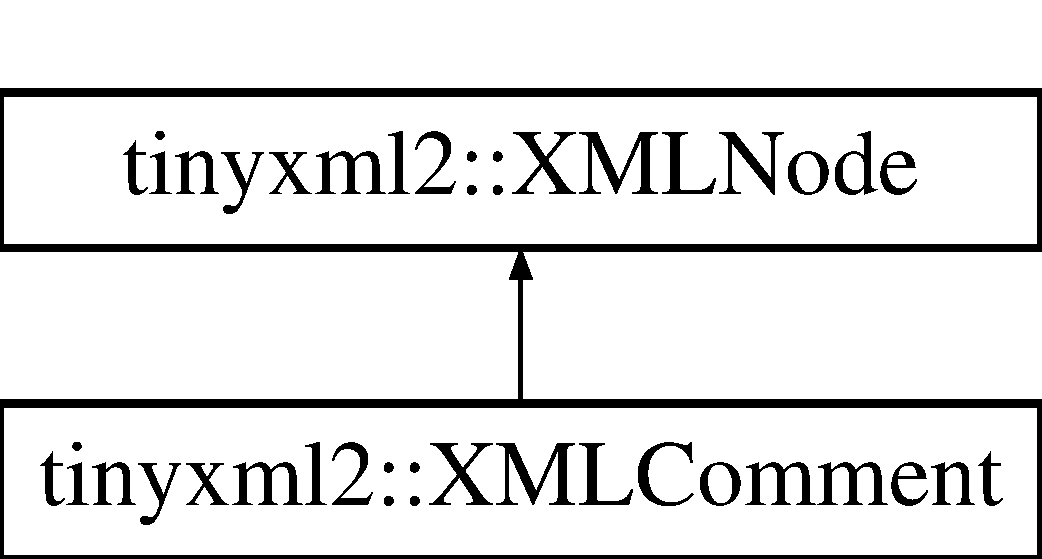
\includegraphics[height=2.000000cm]{classtinyxml2_1_1_x_m_l_comment}
\end{center}
\end{figure}
\subsection*{Public Member Functions}
\begin{DoxyCompactItemize}
\item 
virtual \hyperlink{classtinyxml2_1_1_x_m_l_comment}{X\-M\-L\-Comment} $\ast$ \hyperlink{classtinyxml2_1_1_x_m_l_comment_a8093e1dc8a34fa446d9dc3fde0e6c0ee}{To\-Comment} ()
\begin{DoxyCompactList}\small\item\em Safely cast to a Comment, or null. \end{DoxyCompactList}\item 
virtual const \hyperlink{classtinyxml2_1_1_x_m_l_comment}{X\-M\-L\-Comment} $\ast$ \hyperlink{classtinyxml2_1_1_x_m_l_comment_a422aabac22de7d9c9cad130897dd8b1c}{To\-Comment} () const 
\item 
virtual bool \hyperlink{classtinyxml2_1_1_x_m_l_comment_aa382b1be6a8b0650c16a2d88bb499335}{Accept} (\hyperlink{classtinyxml2_1_1_x_m_l_visitor}{X\-M\-L\-Visitor} $\ast$visitor) const 
\item 
char $\ast$ \hyperlink{classtinyxml2_1_1_x_m_l_comment_aa6ab35c3bb1c1840371dc32a2040c57f}{Parse\-Deep} (char $\ast$, \hyperlink{classtinyxml2_1_1_str_pair}{Str\-Pair} $\ast$end\-Tag)
\item 
virtual \hyperlink{classtinyxml2_1_1_x_m_l_node}{X\-M\-L\-Node} $\ast$ \hyperlink{classtinyxml2_1_1_x_m_l_comment_a90bb60193a691b484f5e1b487857016d}{Shallow\-Clone} (\hyperlink{classtinyxml2_1_1_x_m_l_document}{X\-M\-L\-Document} $\ast$document) const 
\item 
virtual bool \hyperlink{classtinyxml2_1_1_x_m_l_comment_a2d9f26757b0018fce933e74420cda22a}{Shallow\-Equal} (const \hyperlink{classtinyxml2_1_1_x_m_l_node}{X\-M\-L\-Node} $\ast$compare) const 
\end{DoxyCompactItemize}
\subsection*{Protected Member Functions}
\begin{DoxyCompactItemize}
\item 
\hyperlink{classtinyxml2_1_1_x_m_l_comment_ae6463adc3edd93a8e5a9b2b7e99cdf91}{X\-M\-L\-Comment} (\hyperlink{classtinyxml2_1_1_x_m_l_document}{X\-M\-L\-Document} $\ast$doc)
\item 
virtual \hyperlink{classtinyxml2_1_1_x_m_l_comment_ab592f69b47852455c1b32c5e31e453d0}{$\sim$\-X\-M\-L\-Comment} ()
\item 
\hyperlink{classtinyxml2_1_1_x_m_l_comment_aa0a9aae0850ac0e70d3cd20f6cb44447}{X\-M\-L\-Comment} (const \hyperlink{classtinyxml2_1_1_x_m_l_comment}{X\-M\-L\-Comment} \&)
\item 
\hyperlink{classtinyxml2_1_1_x_m_l_comment}{X\-M\-L\-Comment} \& \hyperlink{classtinyxml2_1_1_x_m_l_comment_ac8de55f8381d110740772e6bf6f5755a}{operator=} (const \hyperlink{classtinyxml2_1_1_x_m_l_comment}{X\-M\-L\-Comment} \&)
\end{DoxyCompactItemize}
\subsection*{Friends}
\begin{DoxyCompactItemize}
\item 
class \hyperlink{classtinyxml2_1_1_x_m_l_comment_a4eee3bda60c60a30e4e8cd4ea91c4c6e}{X\-M\-L\-Document}
\end{DoxyCompactItemize}
\subsection*{Additional Inherited Members}


\subsection{Detailed Description}
An X\-M\-L Comment. 

Definition at line 878 of file tinyxml2.\-hpp.



\subsection{Constructor \& Destructor Documentation}
\hypertarget{classtinyxml2_1_1_x_m_l_comment_ae6463adc3edd93a8e5a9b2b7e99cdf91}{\index{tinyxml2\-::\-X\-M\-L\-Comment@{tinyxml2\-::\-X\-M\-L\-Comment}!X\-M\-L\-Comment@{X\-M\-L\-Comment}}
\index{X\-M\-L\-Comment@{X\-M\-L\-Comment}!tinyxml2::XMLComment@{tinyxml2\-::\-X\-M\-L\-Comment}}
\subsubsection[{X\-M\-L\-Comment}]{\setlength{\rightskip}{0pt plus 5cm}tinyxml2\-::\-X\-M\-L\-Comment\-::\-X\-M\-L\-Comment (
\begin{DoxyParamCaption}
\item[{{\bf X\-M\-L\-Document} $\ast$}]{doc}
\end{DoxyParamCaption}
)\hspace{0.3cm}{\ttfamily [protected]}}}\label{classtinyxml2_1_1_x_m_l_comment_ae6463adc3edd93a8e5a9b2b7e99cdf91}


Definition at line 905 of file tinyxml2.\-cpp.

\hypertarget{classtinyxml2_1_1_x_m_l_comment_ab592f69b47852455c1b32c5e31e453d0}{\index{tinyxml2\-::\-X\-M\-L\-Comment@{tinyxml2\-::\-X\-M\-L\-Comment}!$\sim$\-X\-M\-L\-Comment@{$\sim$\-X\-M\-L\-Comment}}
\index{$\sim$\-X\-M\-L\-Comment@{$\sim$\-X\-M\-L\-Comment}!tinyxml2::XMLComment@{tinyxml2\-::\-X\-M\-L\-Comment}}
\subsubsection[{$\sim$\-X\-M\-L\-Comment}]{\setlength{\rightskip}{0pt plus 5cm}tinyxml2\-::\-X\-M\-L\-Comment\-::$\sim$\-X\-M\-L\-Comment (
\begin{DoxyParamCaption}
{}
\end{DoxyParamCaption}
)\hspace{0.3cm}{\ttfamily [protected]}, {\ttfamily [virtual]}}}\label{classtinyxml2_1_1_x_m_l_comment_ab592f69b47852455c1b32c5e31e453d0}


Definition at line 910 of file tinyxml2.\-cpp.

\hypertarget{classtinyxml2_1_1_x_m_l_comment_aa0a9aae0850ac0e70d3cd20f6cb44447}{\index{tinyxml2\-::\-X\-M\-L\-Comment@{tinyxml2\-::\-X\-M\-L\-Comment}!X\-M\-L\-Comment@{X\-M\-L\-Comment}}
\index{X\-M\-L\-Comment@{X\-M\-L\-Comment}!tinyxml2::XMLComment@{tinyxml2\-::\-X\-M\-L\-Comment}}
\subsubsection[{X\-M\-L\-Comment}]{\setlength{\rightskip}{0pt plus 5cm}tinyxml2\-::\-X\-M\-L\-Comment\-::\-X\-M\-L\-Comment (
\begin{DoxyParamCaption}
\item[{const {\bf X\-M\-L\-Comment} \&}]{}
\end{DoxyParamCaption}
)\hspace{0.3cm}{\ttfamily [protected]}}}\label{classtinyxml2_1_1_x_m_l_comment_aa0a9aae0850ac0e70d3cd20f6cb44447}


\subsection{Member Function Documentation}
\hypertarget{classtinyxml2_1_1_x_m_l_comment_aa382b1be6a8b0650c16a2d88bb499335}{\index{tinyxml2\-::\-X\-M\-L\-Comment@{tinyxml2\-::\-X\-M\-L\-Comment}!Accept@{Accept}}
\index{Accept@{Accept}!tinyxml2::XMLComment@{tinyxml2\-::\-X\-M\-L\-Comment}}
\subsubsection[{Accept}]{\setlength{\rightskip}{0pt plus 5cm}bool tinyxml2\-::\-X\-M\-L\-Comment\-::\-Accept (
\begin{DoxyParamCaption}
\item[{{\bf X\-M\-L\-Visitor} $\ast$}]{visitor}
\end{DoxyParamCaption}
) const\hspace{0.3cm}{\ttfamily [virtual]}}}\label{classtinyxml2_1_1_x_m_l_comment_aa382b1be6a8b0650c16a2d88bb499335}
Accept a hierarchical visit of the nodes in the Tiny\-X\-M\-L-\/2 D\-O\-M. Every node in the X\-M\-L tree will be conditionally visited and the host will be called back via the \hyperlink{classtinyxml2_1_1_x_m_l_visitor}{X\-M\-L\-Visitor} interface.

This is essentially a S\-A\-X interface for Tiny\-X\-M\-L-\/2. (Note however it doesn't re-\/parse the X\-M\-L for the callbacks, so the performance of Tiny\-X\-M\-L-\/2 is unchanged by using this interface versus any other.)

The interface has been based on ideas from\-:


\begin{DoxyItemize}
\item \href{http://www.saxproject.org/}{\tt http\-://www.\-saxproject.\-org/}
\item \href{http://c2.com/cgi/wiki?HierarchicalVisitorPattern}{\tt http\-://c2.\-com/cgi/wiki?\-Hierarchical\-Visitor\-Pattern}
\end{DoxyItemize}

Which are both good references for \char`\"{}visiting\char`\"{}.

An example of using \hyperlink{classtinyxml2_1_1_x_m_l_comment_aa382b1be6a8b0650c16a2d88bb499335}{Accept()}\-: \begin{DoxyVerb}XMLPrinter printer;
tinyxmlDoc.Accept( &printer );
const char* xmlcstr = printer.CStr();
\end{DoxyVerb}
 

Implements \hyperlink{classtinyxml2_1_1_x_m_l_node_a81e66df0a44c67a7af17f3b77a152785}{tinyxml2\-::\-X\-M\-L\-Node}.



Definition at line 943 of file tinyxml2.\-cpp.

\hypertarget{classtinyxml2_1_1_x_m_l_comment_ac8de55f8381d110740772e6bf6f5755a}{\index{tinyxml2\-::\-X\-M\-L\-Comment@{tinyxml2\-::\-X\-M\-L\-Comment}!operator=@{operator=}}
\index{operator=@{operator=}!tinyxml2::XMLComment@{tinyxml2\-::\-X\-M\-L\-Comment}}
\subsubsection[{operator=}]{\setlength{\rightskip}{0pt plus 5cm}{\bf X\-M\-L\-Comment}\& tinyxml2\-::\-X\-M\-L\-Comment\-::operator= (
\begin{DoxyParamCaption}
\item[{const {\bf X\-M\-L\-Comment} \&}]{}
\end{DoxyParamCaption}
)\hspace{0.3cm}{\ttfamily [protected]}}}\label{classtinyxml2_1_1_x_m_l_comment_ac8de55f8381d110740772e6bf6f5755a}
\hypertarget{classtinyxml2_1_1_x_m_l_comment_aa6ab35c3bb1c1840371dc32a2040c57f}{\index{tinyxml2\-::\-X\-M\-L\-Comment@{tinyxml2\-::\-X\-M\-L\-Comment}!Parse\-Deep@{Parse\-Deep}}
\index{Parse\-Deep@{Parse\-Deep}!tinyxml2::XMLComment@{tinyxml2\-::\-X\-M\-L\-Comment}}
\subsubsection[{Parse\-Deep}]{\setlength{\rightskip}{0pt plus 5cm}char $\ast$ tinyxml2\-::\-X\-M\-L\-Comment\-::\-Parse\-Deep (
\begin{DoxyParamCaption}
\item[{char $\ast$}]{p, }
\item[{{\bf Str\-Pair} $\ast$}]{end\-Tag}
\end{DoxyParamCaption}
)\hspace{0.3cm}{\ttfamily [virtual]}}}\label{classtinyxml2_1_1_x_m_l_comment_aa6ab35c3bb1c1840371dc32a2040c57f}


Reimplemented from \hyperlink{classtinyxml2_1_1_x_m_l_node_a7610d0f603e8b603d2078521811a23c1}{tinyxml2\-::\-X\-M\-L\-Node}.



Definition at line 915 of file tinyxml2.\-cpp.

\hypertarget{classtinyxml2_1_1_x_m_l_comment_a90bb60193a691b484f5e1b487857016d}{\index{tinyxml2\-::\-X\-M\-L\-Comment@{tinyxml2\-::\-X\-M\-L\-Comment}!Shallow\-Clone@{Shallow\-Clone}}
\index{Shallow\-Clone@{Shallow\-Clone}!tinyxml2::XMLComment@{tinyxml2\-::\-X\-M\-L\-Comment}}
\subsubsection[{Shallow\-Clone}]{\setlength{\rightskip}{0pt plus 5cm}{\bf X\-M\-L\-Node} $\ast$ tinyxml2\-::\-X\-M\-L\-Comment\-::\-Shallow\-Clone (
\begin{DoxyParamCaption}
\item[{{\bf X\-M\-L\-Document} $\ast$}]{document}
\end{DoxyParamCaption}
) const\hspace{0.3cm}{\ttfamily [virtual]}}}\label{classtinyxml2_1_1_x_m_l_comment_a90bb60193a691b484f5e1b487857016d}
Make a copy of this node, but not its children. You may pass in a Document pointer that will be the owner of the new Node. If the 'document' is null, then the node returned will be allocated from the current Document. (this-\/$>$\hyperlink{classtinyxml2_1_1_x_m_l_node_af343d1ef0b45c0020e62d784d7e67a68}{Get\-Document()})

Note\-: if called on a \hyperlink{classtinyxml2_1_1_x_m_l_document}{X\-M\-L\-Document}, this will return null. 

Implements \hyperlink{classtinyxml2_1_1_x_m_l_node_a8402cbd3129d20e9e6024bbcc0531283}{tinyxml2\-::\-X\-M\-L\-Node}.



Definition at line 927 of file tinyxml2.\-cpp.

\hypertarget{classtinyxml2_1_1_x_m_l_comment_a2d9f26757b0018fce933e74420cda22a}{\index{tinyxml2\-::\-X\-M\-L\-Comment@{tinyxml2\-::\-X\-M\-L\-Comment}!Shallow\-Equal@{Shallow\-Equal}}
\index{Shallow\-Equal@{Shallow\-Equal}!tinyxml2::XMLComment@{tinyxml2\-::\-X\-M\-L\-Comment}}
\subsubsection[{Shallow\-Equal}]{\setlength{\rightskip}{0pt plus 5cm}bool tinyxml2\-::\-X\-M\-L\-Comment\-::\-Shallow\-Equal (
\begin{DoxyParamCaption}
\item[{const {\bf X\-M\-L\-Node} $\ast$}]{compare}
\end{DoxyParamCaption}
) const\hspace{0.3cm}{\ttfamily [virtual]}}}\label{classtinyxml2_1_1_x_m_l_comment_a2d9f26757b0018fce933e74420cda22a}
Test if 2 nodes are the same, but don't test children. The 2 nodes do not need to be in the same Document.

Note\-: if called on a \hyperlink{classtinyxml2_1_1_x_m_l_document}{X\-M\-L\-Document}, this will return false. 

Implements \hyperlink{classtinyxml2_1_1_x_m_l_node_a7ce18b751c3ea09eac292dca264f9226}{tinyxml2\-::\-X\-M\-L\-Node}.



Definition at line 937 of file tinyxml2.\-cpp.

\hypertarget{classtinyxml2_1_1_x_m_l_comment_a8093e1dc8a34fa446d9dc3fde0e6c0ee}{\index{tinyxml2\-::\-X\-M\-L\-Comment@{tinyxml2\-::\-X\-M\-L\-Comment}!To\-Comment@{To\-Comment}}
\index{To\-Comment@{To\-Comment}!tinyxml2::XMLComment@{tinyxml2\-::\-X\-M\-L\-Comment}}
\subsubsection[{To\-Comment}]{\setlength{\rightskip}{0pt plus 5cm}virtual {\bf X\-M\-L\-Comment}$\ast$ tinyxml2\-::\-X\-M\-L\-Comment\-::\-To\-Comment (
\begin{DoxyParamCaption}
{}
\end{DoxyParamCaption}
)\hspace{0.3cm}{\ttfamily [inline]}, {\ttfamily [virtual]}}}\label{classtinyxml2_1_1_x_m_l_comment_a8093e1dc8a34fa446d9dc3fde0e6c0ee}


Safely cast to a Comment, or null. 



Reimplemented from \hyperlink{classtinyxml2_1_1_x_m_l_node_aff47671055aa99840a1c1ebd661e63e3}{tinyxml2\-::\-X\-M\-L\-Node}.



Definition at line 882 of file tinyxml2.\-hpp.

\hypertarget{classtinyxml2_1_1_x_m_l_comment_a422aabac22de7d9c9cad130897dd8b1c}{\index{tinyxml2\-::\-X\-M\-L\-Comment@{tinyxml2\-::\-X\-M\-L\-Comment}!To\-Comment@{To\-Comment}}
\index{To\-Comment@{To\-Comment}!tinyxml2::XMLComment@{tinyxml2\-::\-X\-M\-L\-Comment}}
\subsubsection[{To\-Comment}]{\setlength{\rightskip}{0pt plus 5cm}virtual const {\bf X\-M\-L\-Comment}$\ast$ tinyxml2\-::\-X\-M\-L\-Comment\-::\-To\-Comment (
\begin{DoxyParamCaption}
{}
\end{DoxyParamCaption}
) const\hspace{0.3cm}{\ttfamily [inline]}, {\ttfamily [virtual]}}}\label{classtinyxml2_1_1_x_m_l_comment_a422aabac22de7d9c9cad130897dd8b1c}


Reimplemented from \hyperlink{classtinyxml2_1_1_x_m_l_node_a157ce3a00ea5ee5a85b7103138e85e8a}{tinyxml2\-::\-X\-M\-L\-Node}.



Definition at line 885 of file tinyxml2.\-hpp.



\subsection{Friends And Related Function Documentation}
\hypertarget{classtinyxml2_1_1_x_m_l_comment_a4eee3bda60c60a30e4e8cd4ea91c4c6e}{\index{tinyxml2\-::\-X\-M\-L\-Comment@{tinyxml2\-::\-X\-M\-L\-Comment}!X\-M\-L\-Document@{X\-M\-L\-Document}}
\index{X\-M\-L\-Document@{X\-M\-L\-Document}!tinyxml2::XMLComment@{tinyxml2\-::\-X\-M\-L\-Comment}}
\subsubsection[{X\-M\-L\-Document}]{\setlength{\rightskip}{0pt plus 5cm}friend class {\bf X\-M\-L\-Document}\hspace{0.3cm}{\ttfamily [friend]}}}\label{classtinyxml2_1_1_x_m_l_comment_a4eee3bda60c60a30e4e8cd4ea91c4c6e}


Definition at line 880 of file tinyxml2.\-hpp.



The documentation for this class was generated from the following files\-:\begin{DoxyCompactItemize}
\item 
/home/chris/\-Projects/\-Sudden\-Awakening/\-Source/\hyperlink{tinyxml2_8hpp}{tinyxml2.\-hpp}\item 
/home/chris/\-Projects/\-Sudden\-Awakening/\-Source/\hyperlink{tinyxml2_8cpp}{tinyxml2.\-cpp}\end{DoxyCompactItemize}

\hypertarget{classtinyxml2_1_1_x_m_l_const_handle}{\section{tinyxml2\-:\-:X\-M\-L\-Const\-Handle Class Reference}
\label{classtinyxml2_1_1_x_m_l_const_handle}\index{tinyxml2\-::\-X\-M\-L\-Const\-Handle@{tinyxml2\-::\-X\-M\-L\-Const\-Handle}}
}


{\ttfamily \#include $<$tinyxml2.\-hpp$>$}

\subsection*{Public Member Functions}
\begin{DoxyCompactItemize}
\item 
\hyperlink{classtinyxml2_1_1_x_m_l_const_handle_a098bda71fa11d7c74ccddab59d5dd534}{X\-M\-L\-Const\-Handle} (const \hyperlink{classtinyxml2_1_1_x_m_l_node}{X\-M\-L\-Node} $\ast$node)
\item 
\hyperlink{classtinyxml2_1_1_x_m_l_const_handle_a8420a0c4720637e0529e78c2e22f2b0b}{X\-M\-L\-Const\-Handle} (const \hyperlink{classtinyxml2_1_1_x_m_l_node}{X\-M\-L\-Node} \&node)
\item 
\hyperlink{classtinyxml2_1_1_x_m_l_const_handle_a639317ad315ff24f4ef0dc69312d7303}{X\-M\-L\-Const\-Handle} (const \hyperlink{classtinyxml2_1_1_x_m_l_const_handle}{X\-M\-L\-Const\-Handle} \&ref)
\item 
\hyperlink{classtinyxml2_1_1_x_m_l_const_handle}{X\-M\-L\-Const\-Handle} \& \hyperlink{classtinyxml2_1_1_x_m_l_const_handle_a2d74c91df1ff9aa5f9b57e3dceddbf94}{operator=} (const \hyperlink{classtinyxml2_1_1_x_m_l_const_handle}{X\-M\-L\-Const\-Handle} \&ref)
\item 
const \hyperlink{classtinyxml2_1_1_x_m_l_const_handle}{X\-M\-L\-Const\-Handle} \hyperlink{classtinyxml2_1_1_x_m_l_const_handle_a64c4ff7074effc1fd181d68d23f9d1e4}{First\-Child} () const 
\item 
const \hyperlink{classtinyxml2_1_1_x_m_l_const_handle}{X\-M\-L\-Const\-Handle} \hyperlink{classtinyxml2_1_1_x_m_l_const_handle_a5c197d0b57f8e560d93356a4a281469c}{First\-Child\-Element} (const char $\ast$value=0) const 
\item 
const \hyperlink{classtinyxml2_1_1_x_m_l_const_handle}{X\-M\-L\-Const\-Handle} \hyperlink{classtinyxml2_1_1_x_m_l_const_handle_afec9a68e7951193bc5a6e876d602f263}{Last\-Child} () const 
\item 
const \hyperlink{classtinyxml2_1_1_x_m_l_const_handle}{X\-M\-L\-Const\-Handle} \hyperlink{classtinyxml2_1_1_x_m_l_const_handle_a1c400e66dace6fdab4927adb21090059}{Last\-Child\-Element} (const char $\ast$\-\_\-value=0) const 
\item 
const \hyperlink{classtinyxml2_1_1_x_m_l_const_handle}{X\-M\-L\-Const\-Handle} \hyperlink{classtinyxml2_1_1_x_m_l_const_handle_a6917564e26b2c20ebdcb23c7940ad80a}{Previous\-Sibling} () const 
\item 
const \hyperlink{classtinyxml2_1_1_x_m_l_const_handle}{X\-M\-L\-Const\-Handle} \hyperlink{classtinyxml2_1_1_x_m_l_const_handle_acb2e1c5762eff9f6ed72d1a2dfc14271}{Previous\-Sibling\-Element} (const char $\ast$\-\_\-value=0) const 
\item 
const \hyperlink{classtinyxml2_1_1_x_m_l_const_handle}{X\-M\-L\-Const\-Handle} \hyperlink{classtinyxml2_1_1_x_m_l_const_handle_a596e248c8014d718f41658502a2e221b}{Next\-Sibling} () const 
\item 
const \hyperlink{classtinyxml2_1_1_x_m_l_const_handle}{X\-M\-L\-Const\-Handle} \hyperlink{classtinyxml2_1_1_x_m_l_const_handle_a3bbdd3d866c750473bd69a232704503b}{Next\-Sibling\-Element} (const char $\ast$\-\_\-value=0) const 
\item 
const \hyperlink{classtinyxml2_1_1_x_m_l_node}{X\-M\-L\-Node} $\ast$ \hyperlink{classtinyxml2_1_1_x_m_l_const_handle_a95d0256318c10c3f75fa5f8ffb3e4bc1}{To\-Node} () const 
\item 
const \hyperlink{classtinyxml2_1_1_x_m_l_element}{X\-M\-L\-Element} $\ast$ \hyperlink{classtinyxml2_1_1_x_m_l_const_handle_a5a48adefc2a5e70d4ce5b55692a0e2f9}{To\-Element} () const 
\item 
const \hyperlink{classtinyxml2_1_1_x_m_l_text}{X\-M\-L\-Text} $\ast$ \hyperlink{classtinyxml2_1_1_x_m_l_const_handle_ad86ca7dbb20d0495ae357fe7a866e0be}{To\-Text} () const 
\item 
const \hyperlink{classtinyxml2_1_1_x_m_l_unknown}{X\-M\-L\-Unknown} $\ast$ \hyperlink{classtinyxml2_1_1_x_m_l_const_handle_acb358a329e54fa204ed2d0b181566828}{To\-Unknown} () const 
\item 
const \hyperlink{classtinyxml2_1_1_x_m_l_declaration}{X\-M\-L\-Declaration} $\ast$ \hyperlink{classtinyxml2_1_1_x_m_l_const_handle_a5de0c175845bc30a6f9b3d88d8877eaf}{To\-Declaration} () const 
\end{DoxyCompactItemize}


\subsection{Detailed Description}
A variant of the \hyperlink{classtinyxml2_1_1_x_m_l_handle}{X\-M\-L\-Handle} class for working with const X\-M\-L\-Nodes and Documents. It is the same in all regards, except for the 'const' qualifiers. See \hyperlink{classtinyxml2_1_1_x_m_l_handle}{X\-M\-L\-Handle} for A\-P\-I. 

Definition at line 1770 of file tinyxml2.\-hpp.



\subsection{Constructor \& Destructor Documentation}
\hypertarget{classtinyxml2_1_1_x_m_l_const_handle_a098bda71fa11d7c74ccddab59d5dd534}{\index{tinyxml2\-::\-X\-M\-L\-Const\-Handle@{tinyxml2\-::\-X\-M\-L\-Const\-Handle}!X\-M\-L\-Const\-Handle@{X\-M\-L\-Const\-Handle}}
\index{X\-M\-L\-Const\-Handle@{X\-M\-L\-Const\-Handle}!tinyxml2::XMLConstHandle@{tinyxml2\-::\-X\-M\-L\-Const\-Handle}}
\subsubsection[{X\-M\-L\-Const\-Handle}]{\setlength{\rightskip}{0pt plus 5cm}tinyxml2\-::\-X\-M\-L\-Const\-Handle\-::\-X\-M\-L\-Const\-Handle (
\begin{DoxyParamCaption}
\item[{const {\bf X\-M\-L\-Node} $\ast$}]{node}
\end{DoxyParamCaption}
)\hspace{0.3cm}{\ttfamily [inline]}}}\label{classtinyxml2_1_1_x_m_l_const_handle_a098bda71fa11d7c74ccddab59d5dd534}


Definition at line 1773 of file tinyxml2.\-hpp.

\hypertarget{classtinyxml2_1_1_x_m_l_const_handle_a8420a0c4720637e0529e78c2e22f2b0b}{\index{tinyxml2\-::\-X\-M\-L\-Const\-Handle@{tinyxml2\-::\-X\-M\-L\-Const\-Handle}!X\-M\-L\-Const\-Handle@{X\-M\-L\-Const\-Handle}}
\index{X\-M\-L\-Const\-Handle@{X\-M\-L\-Const\-Handle}!tinyxml2::XMLConstHandle@{tinyxml2\-::\-X\-M\-L\-Const\-Handle}}
\subsubsection[{X\-M\-L\-Const\-Handle}]{\setlength{\rightskip}{0pt plus 5cm}tinyxml2\-::\-X\-M\-L\-Const\-Handle\-::\-X\-M\-L\-Const\-Handle (
\begin{DoxyParamCaption}
\item[{const {\bf X\-M\-L\-Node} \&}]{node}
\end{DoxyParamCaption}
)\hspace{0.3cm}{\ttfamily [inline]}}}\label{classtinyxml2_1_1_x_m_l_const_handle_a8420a0c4720637e0529e78c2e22f2b0b}


Definition at line 1776 of file tinyxml2.\-hpp.

\hypertarget{classtinyxml2_1_1_x_m_l_const_handle_a639317ad315ff24f4ef0dc69312d7303}{\index{tinyxml2\-::\-X\-M\-L\-Const\-Handle@{tinyxml2\-::\-X\-M\-L\-Const\-Handle}!X\-M\-L\-Const\-Handle@{X\-M\-L\-Const\-Handle}}
\index{X\-M\-L\-Const\-Handle@{X\-M\-L\-Const\-Handle}!tinyxml2::XMLConstHandle@{tinyxml2\-::\-X\-M\-L\-Const\-Handle}}
\subsubsection[{X\-M\-L\-Const\-Handle}]{\setlength{\rightskip}{0pt plus 5cm}tinyxml2\-::\-X\-M\-L\-Const\-Handle\-::\-X\-M\-L\-Const\-Handle (
\begin{DoxyParamCaption}
\item[{const {\bf X\-M\-L\-Const\-Handle} \&}]{ref}
\end{DoxyParamCaption}
)\hspace{0.3cm}{\ttfamily [inline]}}}\label{classtinyxml2_1_1_x_m_l_const_handle_a639317ad315ff24f4ef0dc69312d7303}


Definition at line 1779 of file tinyxml2.\-hpp.



\subsection{Member Function Documentation}
\hypertarget{classtinyxml2_1_1_x_m_l_const_handle_a64c4ff7074effc1fd181d68d23f9d1e4}{\index{tinyxml2\-::\-X\-M\-L\-Const\-Handle@{tinyxml2\-::\-X\-M\-L\-Const\-Handle}!First\-Child@{First\-Child}}
\index{First\-Child@{First\-Child}!tinyxml2::XMLConstHandle@{tinyxml2\-::\-X\-M\-L\-Const\-Handle}}
\subsubsection[{First\-Child}]{\setlength{\rightskip}{0pt plus 5cm}const {\bf X\-M\-L\-Const\-Handle} tinyxml2\-::\-X\-M\-L\-Const\-Handle\-::\-First\-Child (
\begin{DoxyParamCaption}
{}
\end{DoxyParamCaption}
) const\hspace{0.3cm}{\ttfamily [inline]}}}\label{classtinyxml2_1_1_x_m_l_const_handle_a64c4ff7074effc1fd181d68d23f9d1e4}


Definition at line 1788 of file tinyxml2.\-hpp.

\hypertarget{classtinyxml2_1_1_x_m_l_const_handle_a5c197d0b57f8e560d93356a4a281469c}{\index{tinyxml2\-::\-X\-M\-L\-Const\-Handle@{tinyxml2\-::\-X\-M\-L\-Const\-Handle}!First\-Child\-Element@{First\-Child\-Element}}
\index{First\-Child\-Element@{First\-Child\-Element}!tinyxml2::XMLConstHandle@{tinyxml2\-::\-X\-M\-L\-Const\-Handle}}
\subsubsection[{First\-Child\-Element}]{\setlength{\rightskip}{0pt plus 5cm}const {\bf X\-M\-L\-Const\-Handle} tinyxml2\-::\-X\-M\-L\-Const\-Handle\-::\-First\-Child\-Element (
\begin{DoxyParamCaption}
\item[{const char $\ast$}]{value = {\ttfamily 0}}
\end{DoxyParamCaption}
) const\hspace{0.3cm}{\ttfamily [inline]}}}\label{classtinyxml2_1_1_x_m_l_const_handle_a5c197d0b57f8e560d93356a4a281469c}


Definition at line 1791 of file tinyxml2.\-hpp.

\hypertarget{classtinyxml2_1_1_x_m_l_const_handle_afec9a68e7951193bc5a6e876d602f263}{\index{tinyxml2\-::\-X\-M\-L\-Const\-Handle@{tinyxml2\-::\-X\-M\-L\-Const\-Handle}!Last\-Child@{Last\-Child}}
\index{Last\-Child@{Last\-Child}!tinyxml2::XMLConstHandle@{tinyxml2\-::\-X\-M\-L\-Const\-Handle}}
\subsubsection[{Last\-Child}]{\setlength{\rightskip}{0pt plus 5cm}const {\bf X\-M\-L\-Const\-Handle} tinyxml2\-::\-X\-M\-L\-Const\-Handle\-::\-Last\-Child (
\begin{DoxyParamCaption}
{}
\end{DoxyParamCaption}
) const\hspace{0.3cm}{\ttfamily [inline]}}}\label{classtinyxml2_1_1_x_m_l_const_handle_afec9a68e7951193bc5a6e876d602f263}


Definition at line 1794 of file tinyxml2.\-hpp.

\hypertarget{classtinyxml2_1_1_x_m_l_const_handle_a1c400e66dace6fdab4927adb21090059}{\index{tinyxml2\-::\-X\-M\-L\-Const\-Handle@{tinyxml2\-::\-X\-M\-L\-Const\-Handle}!Last\-Child\-Element@{Last\-Child\-Element}}
\index{Last\-Child\-Element@{Last\-Child\-Element}!tinyxml2::XMLConstHandle@{tinyxml2\-::\-X\-M\-L\-Const\-Handle}}
\subsubsection[{Last\-Child\-Element}]{\setlength{\rightskip}{0pt plus 5cm}const {\bf X\-M\-L\-Const\-Handle} tinyxml2\-::\-X\-M\-L\-Const\-Handle\-::\-Last\-Child\-Element (
\begin{DoxyParamCaption}
\item[{const char $\ast$}]{\-\_\-value = {\ttfamily 0}}
\end{DoxyParamCaption}
) const\hspace{0.3cm}{\ttfamily [inline]}}}\label{classtinyxml2_1_1_x_m_l_const_handle_a1c400e66dace6fdab4927adb21090059}


Definition at line 1797 of file tinyxml2.\-hpp.

\hypertarget{classtinyxml2_1_1_x_m_l_const_handle_a596e248c8014d718f41658502a2e221b}{\index{tinyxml2\-::\-X\-M\-L\-Const\-Handle@{tinyxml2\-::\-X\-M\-L\-Const\-Handle}!Next\-Sibling@{Next\-Sibling}}
\index{Next\-Sibling@{Next\-Sibling}!tinyxml2::XMLConstHandle@{tinyxml2\-::\-X\-M\-L\-Const\-Handle}}
\subsubsection[{Next\-Sibling}]{\setlength{\rightskip}{0pt plus 5cm}const {\bf X\-M\-L\-Const\-Handle} tinyxml2\-::\-X\-M\-L\-Const\-Handle\-::\-Next\-Sibling (
\begin{DoxyParamCaption}
{}
\end{DoxyParamCaption}
) const\hspace{0.3cm}{\ttfamily [inline]}}}\label{classtinyxml2_1_1_x_m_l_const_handle_a596e248c8014d718f41658502a2e221b}


Definition at line 1806 of file tinyxml2.\-hpp.

\hypertarget{classtinyxml2_1_1_x_m_l_const_handle_a3bbdd3d866c750473bd69a232704503b}{\index{tinyxml2\-::\-X\-M\-L\-Const\-Handle@{tinyxml2\-::\-X\-M\-L\-Const\-Handle}!Next\-Sibling\-Element@{Next\-Sibling\-Element}}
\index{Next\-Sibling\-Element@{Next\-Sibling\-Element}!tinyxml2::XMLConstHandle@{tinyxml2\-::\-X\-M\-L\-Const\-Handle}}
\subsubsection[{Next\-Sibling\-Element}]{\setlength{\rightskip}{0pt plus 5cm}const {\bf X\-M\-L\-Const\-Handle} tinyxml2\-::\-X\-M\-L\-Const\-Handle\-::\-Next\-Sibling\-Element (
\begin{DoxyParamCaption}
\item[{const char $\ast$}]{\-\_\-value = {\ttfamily 0}}
\end{DoxyParamCaption}
) const\hspace{0.3cm}{\ttfamily [inline]}}}\label{classtinyxml2_1_1_x_m_l_const_handle_a3bbdd3d866c750473bd69a232704503b}


Definition at line 1809 of file tinyxml2.\-hpp.

\hypertarget{classtinyxml2_1_1_x_m_l_const_handle_a2d74c91df1ff9aa5f9b57e3dceddbf94}{\index{tinyxml2\-::\-X\-M\-L\-Const\-Handle@{tinyxml2\-::\-X\-M\-L\-Const\-Handle}!operator=@{operator=}}
\index{operator=@{operator=}!tinyxml2::XMLConstHandle@{tinyxml2\-::\-X\-M\-L\-Const\-Handle}}
\subsubsection[{operator=}]{\setlength{\rightskip}{0pt plus 5cm}{\bf X\-M\-L\-Const\-Handle}\& tinyxml2\-::\-X\-M\-L\-Const\-Handle\-::operator= (
\begin{DoxyParamCaption}
\item[{const {\bf X\-M\-L\-Const\-Handle} \&}]{ref}
\end{DoxyParamCaption}
)\hspace{0.3cm}{\ttfamily [inline]}}}\label{classtinyxml2_1_1_x_m_l_const_handle_a2d74c91df1ff9aa5f9b57e3dceddbf94}


Definition at line 1783 of file tinyxml2.\-hpp.

\hypertarget{classtinyxml2_1_1_x_m_l_const_handle_a6917564e26b2c20ebdcb23c7940ad80a}{\index{tinyxml2\-::\-X\-M\-L\-Const\-Handle@{tinyxml2\-::\-X\-M\-L\-Const\-Handle}!Previous\-Sibling@{Previous\-Sibling}}
\index{Previous\-Sibling@{Previous\-Sibling}!tinyxml2::XMLConstHandle@{tinyxml2\-::\-X\-M\-L\-Const\-Handle}}
\subsubsection[{Previous\-Sibling}]{\setlength{\rightskip}{0pt plus 5cm}const {\bf X\-M\-L\-Const\-Handle} tinyxml2\-::\-X\-M\-L\-Const\-Handle\-::\-Previous\-Sibling (
\begin{DoxyParamCaption}
{}
\end{DoxyParamCaption}
) const\hspace{0.3cm}{\ttfamily [inline]}}}\label{classtinyxml2_1_1_x_m_l_const_handle_a6917564e26b2c20ebdcb23c7940ad80a}


Definition at line 1800 of file tinyxml2.\-hpp.

\hypertarget{classtinyxml2_1_1_x_m_l_const_handle_acb2e1c5762eff9f6ed72d1a2dfc14271}{\index{tinyxml2\-::\-X\-M\-L\-Const\-Handle@{tinyxml2\-::\-X\-M\-L\-Const\-Handle}!Previous\-Sibling\-Element@{Previous\-Sibling\-Element}}
\index{Previous\-Sibling\-Element@{Previous\-Sibling\-Element}!tinyxml2::XMLConstHandle@{tinyxml2\-::\-X\-M\-L\-Const\-Handle}}
\subsubsection[{Previous\-Sibling\-Element}]{\setlength{\rightskip}{0pt plus 5cm}const {\bf X\-M\-L\-Const\-Handle} tinyxml2\-::\-X\-M\-L\-Const\-Handle\-::\-Previous\-Sibling\-Element (
\begin{DoxyParamCaption}
\item[{const char $\ast$}]{\-\_\-value = {\ttfamily 0}}
\end{DoxyParamCaption}
) const\hspace{0.3cm}{\ttfamily [inline]}}}\label{classtinyxml2_1_1_x_m_l_const_handle_acb2e1c5762eff9f6ed72d1a2dfc14271}


Definition at line 1803 of file tinyxml2.\-hpp.

\hypertarget{classtinyxml2_1_1_x_m_l_const_handle_a5de0c175845bc30a6f9b3d88d8877eaf}{\index{tinyxml2\-::\-X\-M\-L\-Const\-Handle@{tinyxml2\-::\-X\-M\-L\-Const\-Handle}!To\-Declaration@{To\-Declaration}}
\index{To\-Declaration@{To\-Declaration}!tinyxml2::XMLConstHandle@{tinyxml2\-::\-X\-M\-L\-Const\-Handle}}
\subsubsection[{To\-Declaration}]{\setlength{\rightskip}{0pt plus 5cm}const {\bf X\-M\-L\-Declaration}$\ast$ tinyxml2\-::\-X\-M\-L\-Const\-Handle\-::\-To\-Declaration (
\begin{DoxyParamCaption}
{}
\end{DoxyParamCaption}
) const\hspace{0.3cm}{\ttfamily [inline]}}}\label{classtinyxml2_1_1_x_m_l_const_handle_a5de0c175845bc30a6f9b3d88d8877eaf}


Definition at line 1826 of file tinyxml2.\-hpp.

\hypertarget{classtinyxml2_1_1_x_m_l_const_handle_a5a48adefc2a5e70d4ce5b55692a0e2f9}{\index{tinyxml2\-::\-X\-M\-L\-Const\-Handle@{tinyxml2\-::\-X\-M\-L\-Const\-Handle}!To\-Element@{To\-Element}}
\index{To\-Element@{To\-Element}!tinyxml2::XMLConstHandle@{tinyxml2\-::\-X\-M\-L\-Const\-Handle}}
\subsubsection[{To\-Element}]{\setlength{\rightskip}{0pt plus 5cm}const {\bf X\-M\-L\-Element}$\ast$ tinyxml2\-::\-X\-M\-L\-Const\-Handle\-::\-To\-Element (
\begin{DoxyParamCaption}
{}
\end{DoxyParamCaption}
) const\hspace{0.3cm}{\ttfamily [inline]}}}\label{classtinyxml2_1_1_x_m_l_const_handle_a5a48adefc2a5e70d4ce5b55692a0e2f9}


Definition at line 1817 of file tinyxml2.\-hpp.

\hypertarget{classtinyxml2_1_1_x_m_l_const_handle_a95d0256318c10c3f75fa5f8ffb3e4bc1}{\index{tinyxml2\-::\-X\-M\-L\-Const\-Handle@{tinyxml2\-::\-X\-M\-L\-Const\-Handle}!To\-Node@{To\-Node}}
\index{To\-Node@{To\-Node}!tinyxml2::XMLConstHandle@{tinyxml2\-::\-X\-M\-L\-Const\-Handle}}
\subsubsection[{To\-Node}]{\setlength{\rightskip}{0pt plus 5cm}const {\bf X\-M\-L\-Node}$\ast$ tinyxml2\-::\-X\-M\-L\-Const\-Handle\-::\-To\-Node (
\begin{DoxyParamCaption}
{}
\end{DoxyParamCaption}
) const\hspace{0.3cm}{\ttfamily [inline]}}}\label{classtinyxml2_1_1_x_m_l_const_handle_a95d0256318c10c3f75fa5f8ffb3e4bc1}


Definition at line 1814 of file tinyxml2.\-hpp.

\hypertarget{classtinyxml2_1_1_x_m_l_const_handle_ad86ca7dbb20d0495ae357fe7a866e0be}{\index{tinyxml2\-::\-X\-M\-L\-Const\-Handle@{tinyxml2\-::\-X\-M\-L\-Const\-Handle}!To\-Text@{To\-Text}}
\index{To\-Text@{To\-Text}!tinyxml2::XMLConstHandle@{tinyxml2\-::\-X\-M\-L\-Const\-Handle}}
\subsubsection[{To\-Text}]{\setlength{\rightskip}{0pt plus 5cm}const {\bf X\-M\-L\-Text}$\ast$ tinyxml2\-::\-X\-M\-L\-Const\-Handle\-::\-To\-Text (
\begin{DoxyParamCaption}
{}
\end{DoxyParamCaption}
) const\hspace{0.3cm}{\ttfamily [inline]}}}\label{classtinyxml2_1_1_x_m_l_const_handle_ad86ca7dbb20d0495ae357fe7a866e0be}


Definition at line 1820 of file tinyxml2.\-hpp.

\hypertarget{classtinyxml2_1_1_x_m_l_const_handle_acb358a329e54fa204ed2d0b181566828}{\index{tinyxml2\-::\-X\-M\-L\-Const\-Handle@{tinyxml2\-::\-X\-M\-L\-Const\-Handle}!To\-Unknown@{To\-Unknown}}
\index{To\-Unknown@{To\-Unknown}!tinyxml2::XMLConstHandle@{tinyxml2\-::\-X\-M\-L\-Const\-Handle}}
\subsubsection[{To\-Unknown}]{\setlength{\rightskip}{0pt plus 5cm}const {\bf X\-M\-L\-Unknown}$\ast$ tinyxml2\-::\-X\-M\-L\-Const\-Handle\-::\-To\-Unknown (
\begin{DoxyParamCaption}
{}
\end{DoxyParamCaption}
) const\hspace{0.3cm}{\ttfamily [inline]}}}\label{classtinyxml2_1_1_x_m_l_const_handle_acb358a329e54fa204ed2d0b181566828}


Definition at line 1823 of file tinyxml2.\-hpp.



The documentation for this class was generated from the following file\-:\begin{DoxyCompactItemize}
\item 
/home/chris/\-Projects/\-Sudden\-Awakening/\-Source/\hyperlink{tinyxml2_8hpp}{tinyxml2.\-hpp}\end{DoxyCompactItemize}

\hypertarget{classtinyxml2_1_1_x_m_l_declaration}{\section{tinyxml2\-:\-:X\-M\-L\-Declaration Class Reference}
\label{classtinyxml2_1_1_x_m_l_declaration}\index{tinyxml2\-::\-X\-M\-L\-Declaration@{tinyxml2\-::\-X\-M\-L\-Declaration}}
}


{\ttfamily \#include $<$tinyxml2.\-hpp$>$}

Inheritance diagram for tinyxml2\-:\-:X\-M\-L\-Declaration\-:\begin{figure}[H]
\begin{center}
\leavevmode
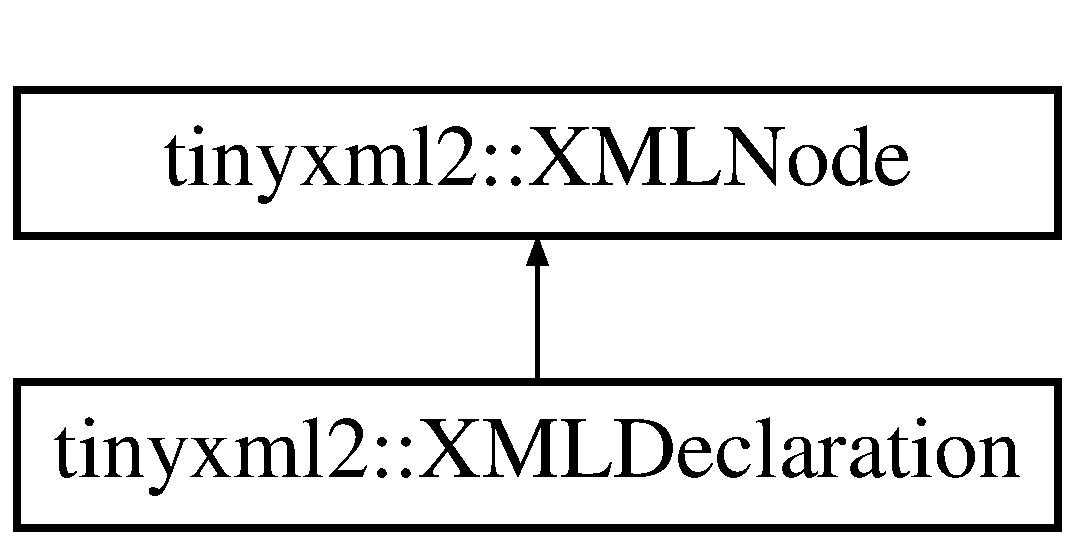
\includegraphics[height=2.000000cm]{classtinyxml2_1_1_x_m_l_declaration}
\end{center}
\end{figure}
\subsection*{Public Member Functions}
\begin{DoxyCompactItemize}
\item 
virtual \hyperlink{classtinyxml2_1_1_x_m_l_declaration}{X\-M\-L\-Declaration} $\ast$ \hyperlink{classtinyxml2_1_1_x_m_l_declaration_a159d8ac45865215e88059ea1e5b52fc5}{To\-Declaration} ()
\begin{DoxyCompactList}\small\item\em Safely cast to a Declaration, or null. \end{DoxyCompactList}\item 
virtual const \hyperlink{classtinyxml2_1_1_x_m_l_declaration}{X\-M\-L\-Declaration} $\ast$ \hyperlink{classtinyxml2_1_1_x_m_l_declaration_af724607a5fa810496fd6a21f5975a643}{To\-Declaration} () const 
\item 
virtual bool \hyperlink{classtinyxml2_1_1_x_m_l_declaration_a953a7359cc312d15218eb5843a4ca108}{Accept} (\hyperlink{classtinyxml2_1_1_x_m_l_visitor}{X\-M\-L\-Visitor} $\ast$visitor) const 
\item 
char $\ast$ \hyperlink{classtinyxml2_1_1_x_m_l_declaration_a19e33e0a9f9500f449261558c36f9a44}{Parse\-Deep} (char $\ast$, \hyperlink{classtinyxml2_1_1_str_pair}{Str\-Pair} $\ast$end\-Tag)
\item 
virtual \hyperlink{classtinyxml2_1_1_x_m_l_node}{X\-M\-L\-Node} $\ast$ \hyperlink{classtinyxml2_1_1_x_m_l_declaration_a39458732ee6796cfc85dd35d3c488e0b}{Shallow\-Clone} (\hyperlink{classtinyxml2_1_1_x_m_l_document}{X\-M\-L\-Document} $\ast$document) const 
\item 
virtual bool \hyperlink{classtinyxml2_1_1_x_m_l_declaration_ace0d2d9bc1b63278bd5e984ebe0c7bd0}{Shallow\-Equal} (const \hyperlink{classtinyxml2_1_1_x_m_l_node}{X\-M\-L\-Node} $\ast$compare) const 
\end{DoxyCompactItemize}
\subsection*{Protected Member Functions}
\begin{DoxyCompactItemize}
\item 
\hyperlink{classtinyxml2_1_1_x_m_l_declaration_aef9586f2ce5df5feba74dde49a242b06}{X\-M\-L\-Declaration} (\hyperlink{classtinyxml2_1_1_x_m_l_document}{X\-M\-L\-Document} $\ast$doc)
\item 
virtual \hyperlink{classtinyxml2_1_1_x_m_l_declaration_ab93d5bf4f5d58b4144963cf739cf6dcc}{$\sim$\-X\-M\-L\-Declaration} ()
\item 
\hyperlink{classtinyxml2_1_1_x_m_l_declaration_a5229cc0b31f034f93289af27ec3e2836}{X\-M\-L\-Declaration} (const \hyperlink{classtinyxml2_1_1_x_m_l_declaration}{X\-M\-L\-Declaration} \&)
\item 
\hyperlink{classtinyxml2_1_1_x_m_l_declaration}{X\-M\-L\-Declaration} \& \hyperlink{classtinyxml2_1_1_x_m_l_declaration_a79eb518c2c2b1b99a122a5d5a308b7ee}{operator=} (const \hyperlink{classtinyxml2_1_1_x_m_l_declaration}{X\-M\-L\-Declaration} \&)
\end{DoxyCompactItemize}
\subsection*{Friends}
\begin{DoxyCompactItemize}
\item 
class \hyperlink{classtinyxml2_1_1_x_m_l_declaration_a4eee3bda60c60a30e4e8cd4ea91c4c6e}{X\-M\-L\-Document}
\end{DoxyCompactItemize}
\subsection*{Additional Inherited Members}


\subsection{Detailed Description}
In correct X\-M\-L the declaration is the first entry in the file. \begin{DoxyVerb}    <?xml version="1.0" standalone="yes"?>
\end{DoxyVerb}


Tiny\-X\-M\-L-\/2 will happily read or write files without a declaration, however.

The text of the declaration isn't interpreted. It is parsed and written as a string. 

Definition at line 916 of file tinyxml2.\-hpp.



\subsection{Constructor \& Destructor Documentation}
\hypertarget{classtinyxml2_1_1_x_m_l_declaration_aef9586f2ce5df5feba74dde49a242b06}{\index{tinyxml2\-::\-X\-M\-L\-Declaration@{tinyxml2\-::\-X\-M\-L\-Declaration}!X\-M\-L\-Declaration@{X\-M\-L\-Declaration}}
\index{X\-M\-L\-Declaration@{X\-M\-L\-Declaration}!tinyxml2::XMLDeclaration@{tinyxml2\-::\-X\-M\-L\-Declaration}}
\subsubsection[{X\-M\-L\-Declaration}]{\setlength{\rightskip}{0pt plus 5cm}tinyxml2\-::\-X\-M\-L\-Declaration\-::\-X\-M\-L\-Declaration (
\begin{DoxyParamCaption}
\item[{{\bf X\-M\-L\-Document} $\ast$}]{doc}
\end{DoxyParamCaption}
)\hspace{0.3cm}{\ttfamily [protected]}}}\label{classtinyxml2_1_1_x_m_l_declaration_aef9586f2ce5df5feba74dde49a242b06}


Definition at line 951 of file tinyxml2.\-cpp.

\hypertarget{classtinyxml2_1_1_x_m_l_declaration_ab93d5bf4f5d58b4144963cf739cf6dcc}{\index{tinyxml2\-::\-X\-M\-L\-Declaration@{tinyxml2\-::\-X\-M\-L\-Declaration}!$\sim$\-X\-M\-L\-Declaration@{$\sim$\-X\-M\-L\-Declaration}}
\index{$\sim$\-X\-M\-L\-Declaration@{$\sim$\-X\-M\-L\-Declaration}!tinyxml2::XMLDeclaration@{tinyxml2\-::\-X\-M\-L\-Declaration}}
\subsubsection[{$\sim$\-X\-M\-L\-Declaration}]{\setlength{\rightskip}{0pt plus 5cm}tinyxml2\-::\-X\-M\-L\-Declaration\-::$\sim$\-X\-M\-L\-Declaration (
\begin{DoxyParamCaption}
{}
\end{DoxyParamCaption}
)\hspace{0.3cm}{\ttfamily [protected]}, {\ttfamily [virtual]}}}\label{classtinyxml2_1_1_x_m_l_declaration_ab93d5bf4f5d58b4144963cf739cf6dcc}


Definition at line 956 of file tinyxml2.\-cpp.

\hypertarget{classtinyxml2_1_1_x_m_l_declaration_a5229cc0b31f034f93289af27ec3e2836}{\index{tinyxml2\-::\-X\-M\-L\-Declaration@{tinyxml2\-::\-X\-M\-L\-Declaration}!X\-M\-L\-Declaration@{X\-M\-L\-Declaration}}
\index{X\-M\-L\-Declaration@{X\-M\-L\-Declaration}!tinyxml2::XMLDeclaration@{tinyxml2\-::\-X\-M\-L\-Declaration}}
\subsubsection[{X\-M\-L\-Declaration}]{\setlength{\rightskip}{0pt plus 5cm}tinyxml2\-::\-X\-M\-L\-Declaration\-::\-X\-M\-L\-Declaration (
\begin{DoxyParamCaption}
\item[{const {\bf X\-M\-L\-Declaration} \&}]{}
\end{DoxyParamCaption}
)\hspace{0.3cm}{\ttfamily [protected]}}}\label{classtinyxml2_1_1_x_m_l_declaration_a5229cc0b31f034f93289af27ec3e2836}


\subsection{Member Function Documentation}
\hypertarget{classtinyxml2_1_1_x_m_l_declaration_a953a7359cc312d15218eb5843a4ca108}{\index{tinyxml2\-::\-X\-M\-L\-Declaration@{tinyxml2\-::\-X\-M\-L\-Declaration}!Accept@{Accept}}
\index{Accept@{Accept}!tinyxml2::XMLDeclaration@{tinyxml2\-::\-X\-M\-L\-Declaration}}
\subsubsection[{Accept}]{\setlength{\rightskip}{0pt plus 5cm}bool tinyxml2\-::\-X\-M\-L\-Declaration\-::\-Accept (
\begin{DoxyParamCaption}
\item[{{\bf X\-M\-L\-Visitor} $\ast$}]{visitor}
\end{DoxyParamCaption}
) const\hspace{0.3cm}{\ttfamily [virtual]}}}\label{classtinyxml2_1_1_x_m_l_declaration_a953a7359cc312d15218eb5843a4ca108}
Accept a hierarchical visit of the nodes in the Tiny\-X\-M\-L-\/2 D\-O\-M. Every node in the X\-M\-L tree will be conditionally visited and the host will be called back via the \hyperlink{classtinyxml2_1_1_x_m_l_visitor}{X\-M\-L\-Visitor} interface.

This is essentially a S\-A\-X interface for Tiny\-X\-M\-L-\/2. (Note however it doesn't re-\/parse the X\-M\-L for the callbacks, so the performance of Tiny\-X\-M\-L-\/2 is unchanged by using this interface versus any other.)

The interface has been based on ideas from\-:


\begin{DoxyItemize}
\item \href{http://www.saxproject.org/}{\tt http\-://www.\-saxproject.\-org/}
\item \href{http://c2.com/cgi/wiki?HierarchicalVisitorPattern}{\tt http\-://c2.\-com/cgi/wiki?\-Hierarchical\-Visitor\-Pattern}
\end{DoxyItemize}

Which are both good references for \char`\"{}visiting\char`\"{}.

An example of using \hyperlink{classtinyxml2_1_1_x_m_l_declaration_a953a7359cc312d15218eb5843a4ca108}{Accept()}\-: \begin{DoxyVerb}XMLPrinter printer;
tinyxmlDoc.Accept( &printer );
const char* xmlcstr = printer.CStr();
\end{DoxyVerb}
 

Implements \hyperlink{classtinyxml2_1_1_x_m_l_node_a81e66df0a44c67a7af17f3b77a152785}{tinyxml2\-::\-X\-M\-L\-Node}.



Definition at line 991 of file tinyxml2.\-cpp.

\hypertarget{classtinyxml2_1_1_x_m_l_declaration_a79eb518c2c2b1b99a122a5d5a308b7ee}{\index{tinyxml2\-::\-X\-M\-L\-Declaration@{tinyxml2\-::\-X\-M\-L\-Declaration}!operator=@{operator=}}
\index{operator=@{operator=}!tinyxml2::XMLDeclaration@{tinyxml2\-::\-X\-M\-L\-Declaration}}
\subsubsection[{operator=}]{\setlength{\rightskip}{0pt plus 5cm}{\bf X\-M\-L\-Declaration}\& tinyxml2\-::\-X\-M\-L\-Declaration\-::operator= (
\begin{DoxyParamCaption}
\item[{const {\bf X\-M\-L\-Declaration} \&}]{}
\end{DoxyParamCaption}
)\hspace{0.3cm}{\ttfamily [protected]}}}\label{classtinyxml2_1_1_x_m_l_declaration_a79eb518c2c2b1b99a122a5d5a308b7ee}
\hypertarget{classtinyxml2_1_1_x_m_l_declaration_a19e33e0a9f9500f449261558c36f9a44}{\index{tinyxml2\-::\-X\-M\-L\-Declaration@{tinyxml2\-::\-X\-M\-L\-Declaration}!Parse\-Deep@{Parse\-Deep}}
\index{Parse\-Deep@{Parse\-Deep}!tinyxml2::XMLDeclaration@{tinyxml2\-::\-X\-M\-L\-Declaration}}
\subsubsection[{Parse\-Deep}]{\setlength{\rightskip}{0pt plus 5cm}char $\ast$ tinyxml2\-::\-X\-M\-L\-Declaration\-::\-Parse\-Deep (
\begin{DoxyParamCaption}
\item[{char $\ast$}]{p, }
\item[{{\bf Str\-Pair} $\ast$}]{end\-Tag}
\end{DoxyParamCaption}
)\hspace{0.3cm}{\ttfamily [virtual]}}}\label{classtinyxml2_1_1_x_m_l_declaration_a19e33e0a9f9500f449261558c36f9a44}


Reimplemented from \hyperlink{classtinyxml2_1_1_x_m_l_node_a7610d0f603e8b603d2078521811a23c1}{tinyxml2\-::\-X\-M\-L\-Node}.



Definition at line 962 of file tinyxml2.\-cpp.

\hypertarget{classtinyxml2_1_1_x_m_l_declaration_a39458732ee6796cfc85dd35d3c488e0b}{\index{tinyxml2\-::\-X\-M\-L\-Declaration@{tinyxml2\-::\-X\-M\-L\-Declaration}!Shallow\-Clone@{Shallow\-Clone}}
\index{Shallow\-Clone@{Shallow\-Clone}!tinyxml2::XMLDeclaration@{tinyxml2\-::\-X\-M\-L\-Declaration}}
\subsubsection[{Shallow\-Clone}]{\setlength{\rightskip}{0pt plus 5cm}{\bf X\-M\-L\-Node} $\ast$ tinyxml2\-::\-X\-M\-L\-Declaration\-::\-Shallow\-Clone (
\begin{DoxyParamCaption}
\item[{{\bf X\-M\-L\-Document} $\ast$}]{document}
\end{DoxyParamCaption}
) const\hspace{0.3cm}{\ttfamily [virtual]}}}\label{classtinyxml2_1_1_x_m_l_declaration_a39458732ee6796cfc85dd35d3c488e0b}
Make a copy of this node, but not its children. You may pass in a Document pointer that will be the owner of the new Node. If the 'document' is null, then the node returned will be allocated from the current Document. (this-\/$>$\hyperlink{classtinyxml2_1_1_x_m_l_node_af343d1ef0b45c0020e62d784d7e67a68}{Get\-Document()})

Note\-: if called on a \hyperlink{classtinyxml2_1_1_x_m_l_document}{X\-M\-L\-Document}, this will return null. 

Implements \hyperlink{classtinyxml2_1_1_x_m_l_node_a8402cbd3129d20e9e6024bbcc0531283}{tinyxml2\-::\-X\-M\-L\-Node}.



Definition at line 974 of file tinyxml2.\-cpp.

\hypertarget{classtinyxml2_1_1_x_m_l_declaration_ace0d2d9bc1b63278bd5e984ebe0c7bd0}{\index{tinyxml2\-::\-X\-M\-L\-Declaration@{tinyxml2\-::\-X\-M\-L\-Declaration}!Shallow\-Equal@{Shallow\-Equal}}
\index{Shallow\-Equal@{Shallow\-Equal}!tinyxml2::XMLDeclaration@{tinyxml2\-::\-X\-M\-L\-Declaration}}
\subsubsection[{Shallow\-Equal}]{\setlength{\rightskip}{0pt plus 5cm}bool tinyxml2\-::\-X\-M\-L\-Declaration\-::\-Shallow\-Equal (
\begin{DoxyParamCaption}
\item[{const {\bf X\-M\-L\-Node} $\ast$}]{compare}
\end{DoxyParamCaption}
) const\hspace{0.3cm}{\ttfamily [virtual]}}}\label{classtinyxml2_1_1_x_m_l_declaration_ace0d2d9bc1b63278bd5e984ebe0c7bd0}
Test if 2 nodes are the same, but don't test children. The 2 nodes do not need to be in the same Document.

Note\-: if called on a \hyperlink{classtinyxml2_1_1_x_m_l_document}{X\-M\-L\-Document}, this will return false. 

Implements \hyperlink{classtinyxml2_1_1_x_m_l_node_a7ce18b751c3ea09eac292dca264f9226}{tinyxml2\-::\-X\-M\-L\-Node}.



Definition at line 984 of file tinyxml2.\-cpp.

\hypertarget{classtinyxml2_1_1_x_m_l_declaration_a159d8ac45865215e88059ea1e5b52fc5}{\index{tinyxml2\-::\-X\-M\-L\-Declaration@{tinyxml2\-::\-X\-M\-L\-Declaration}!To\-Declaration@{To\-Declaration}}
\index{To\-Declaration@{To\-Declaration}!tinyxml2::XMLDeclaration@{tinyxml2\-::\-X\-M\-L\-Declaration}}
\subsubsection[{To\-Declaration}]{\setlength{\rightskip}{0pt plus 5cm}virtual {\bf X\-M\-L\-Declaration}$\ast$ tinyxml2\-::\-X\-M\-L\-Declaration\-::\-To\-Declaration (
\begin{DoxyParamCaption}
{}
\end{DoxyParamCaption}
)\hspace{0.3cm}{\ttfamily [inline]}, {\ttfamily [virtual]}}}\label{classtinyxml2_1_1_x_m_l_declaration_a159d8ac45865215e88059ea1e5b52fc5}


Safely cast to a Declaration, or null. 



Reimplemented from \hyperlink{classtinyxml2_1_1_x_m_l_node_a174fd4c22c010b58138c1b84a0dfbd51}{tinyxml2\-::\-X\-M\-L\-Node}.



Definition at line 920 of file tinyxml2.\-hpp.

\hypertarget{classtinyxml2_1_1_x_m_l_declaration_af724607a5fa810496fd6a21f5975a643}{\index{tinyxml2\-::\-X\-M\-L\-Declaration@{tinyxml2\-::\-X\-M\-L\-Declaration}!To\-Declaration@{To\-Declaration}}
\index{To\-Declaration@{To\-Declaration}!tinyxml2::XMLDeclaration@{tinyxml2\-::\-X\-M\-L\-Declaration}}
\subsubsection[{To\-Declaration}]{\setlength{\rightskip}{0pt plus 5cm}virtual const {\bf X\-M\-L\-Declaration}$\ast$ tinyxml2\-::\-X\-M\-L\-Declaration\-::\-To\-Declaration (
\begin{DoxyParamCaption}
{}
\end{DoxyParamCaption}
) const\hspace{0.3cm}{\ttfamily [inline]}, {\ttfamily [virtual]}}}\label{classtinyxml2_1_1_x_m_l_declaration_af724607a5fa810496fd6a21f5975a643}


Reimplemented from \hyperlink{classtinyxml2_1_1_x_m_l_node_aedae0bbb58d533a4b8a61042388b49e5}{tinyxml2\-::\-X\-M\-L\-Node}.



Definition at line 923 of file tinyxml2.\-hpp.



\subsection{Friends And Related Function Documentation}
\hypertarget{classtinyxml2_1_1_x_m_l_declaration_a4eee3bda60c60a30e4e8cd4ea91c4c6e}{\index{tinyxml2\-::\-X\-M\-L\-Declaration@{tinyxml2\-::\-X\-M\-L\-Declaration}!X\-M\-L\-Document@{X\-M\-L\-Document}}
\index{X\-M\-L\-Document@{X\-M\-L\-Document}!tinyxml2::XMLDeclaration@{tinyxml2\-::\-X\-M\-L\-Declaration}}
\subsubsection[{X\-M\-L\-Document}]{\setlength{\rightskip}{0pt plus 5cm}friend class {\bf X\-M\-L\-Document}\hspace{0.3cm}{\ttfamily [friend]}}}\label{classtinyxml2_1_1_x_m_l_declaration_a4eee3bda60c60a30e4e8cd4ea91c4c6e}


Definition at line 918 of file tinyxml2.\-hpp.



The documentation for this class was generated from the following files\-:\begin{DoxyCompactItemize}
\item 
/home/chris/\-Projects/\-Sudden\-Awakening/\-Source/\hyperlink{tinyxml2_8hpp}{tinyxml2.\-hpp}\item 
/home/chris/\-Projects/\-Sudden\-Awakening/\-Source/\hyperlink{tinyxml2_8cpp}{tinyxml2.\-cpp}\end{DoxyCompactItemize}

\hypertarget{classtinyxml2_1_1_x_m_l_document}{\section{tinyxml2\-:\-:X\-M\-L\-Document Class Reference}
\label{classtinyxml2_1_1_x_m_l_document}\index{tinyxml2\-::\-X\-M\-L\-Document@{tinyxml2\-::\-X\-M\-L\-Document}}
}


{\ttfamily \#include $<$tinyxml2.\-hpp$>$}

Inheritance diagram for tinyxml2\-:\-:X\-M\-L\-Document\-:\begin{figure}[H]
\begin{center}
\leavevmode
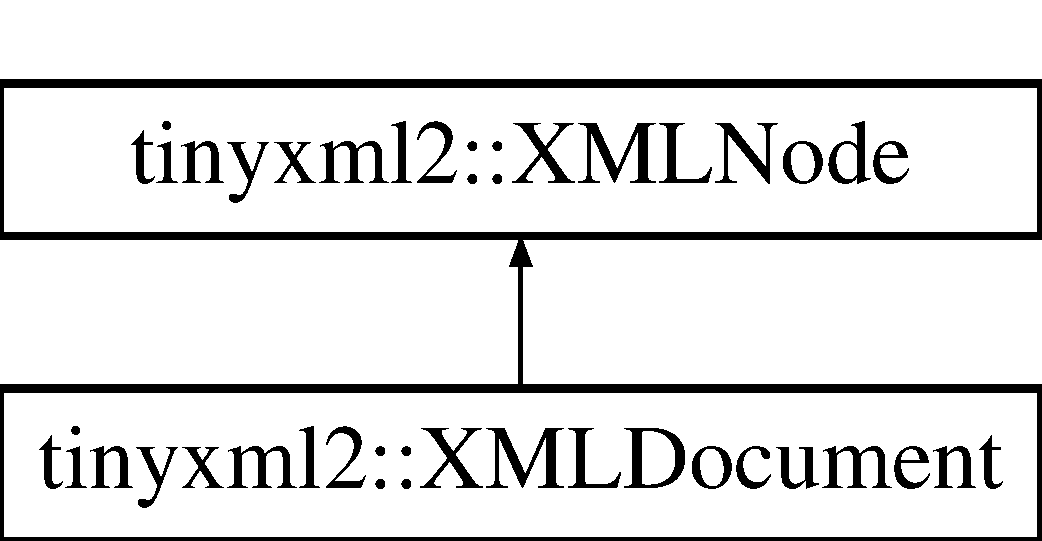
\includegraphics[height=2.000000cm]{classtinyxml2_1_1_x_m_l_document}
\end{center}
\end{figure}
\subsection*{Public Member Functions}
\begin{DoxyCompactItemize}
\item 
\hyperlink{classtinyxml2_1_1_x_m_l_document_af1574f76ebb619f25ef3f09eb2ba5188}{X\-M\-L\-Document} (bool process\-Entities=true, \hyperlink{namespacetinyxml2_a7f91d00f77360f850fd5da0861e27dd5}{Whitespace}=\hyperlink{namespacetinyxml2_a7f91d00f77360f850fd5da0861e27dd5a751769aa625fe5fe5286e9779edec56a}{P\-R\-E\-S\-E\-R\-V\-E\-\_\-\-W\-H\-I\-T\-E\-S\-P\-A\-C\-E})
\begin{DoxyCompactList}\small\item\em constructor \end{DoxyCompactList}\item 
\hyperlink{classtinyxml2_1_1_x_m_l_document_af37c47d8e2ba4b2fc81b21a77a32579b}{$\sim$\-X\-M\-L\-Document} ()
\item 
virtual \hyperlink{classtinyxml2_1_1_x_m_l_document}{X\-M\-L\-Document} $\ast$ \hyperlink{classtinyxml2_1_1_x_m_l_document_a3e185f880882bd978367bb55937735ec}{To\-Document} ()
\begin{DoxyCompactList}\small\item\em Safely cast to a Document, or null. \end{DoxyCompactList}\item 
virtual const \hyperlink{classtinyxml2_1_1_x_m_l_document}{X\-M\-L\-Document} $\ast$ \hyperlink{classtinyxml2_1_1_x_m_l_document_a15eb1a62afa18c66808031da647d1129}{To\-Document} () const 
\item 
\hyperlink{namespacetinyxml2_a1fbf88509c3ac88c09117b1947414e08}{X\-M\-L\-Error} \hyperlink{classtinyxml2_1_1_x_m_l_document_a1819bd34f540a7304c105a6232d25a1f}{Parse} (const char $\ast$xml, size\-\_\-t n\-Bytes=(size\-\_\-t)(-\/1))
\item 
\hyperlink{namespacetinyxml2_a1fbf88509c3ac88c09117b1947414e08}{X\-M\-L\-Error} \hyperlink{classtinyxml2_1_1_x_m_l_document_a2ebd4647a8af5fc6831b294ac26a150a}{Load\-File} (const char $\ast$filename)
\item 
\hyperlink{namespacetinyxml2_a1fbf88509c3ac88c09117b1947414e08}{X\-M\-L\-Error} \hyperlink{classtinyxml2_1_1_x_m_l_document_a5f1d330fad44c52f3d265338dd2a6dc2}{Load\-File} (F\-I\-L\-E $\ast$)
\item 
\hyperlink{namespacetinyxml2_a1fbf88509c3ac88c09117b1947414e08}{X\-M\-L\-Error} \hyperlink{classtinyxml2_1_1_x_m_l_document_a73ac416b4a2aa0952e841220eb3da18f}{Save\-File} (const char $\ast$filename, bool compact=false)
\item 
\hyperlink{namespacetinyxml2_a1fbf88509c3ac88c09117b1947414e08}{X\-M\-L\-Error} \hyperlink{classtinyxml2_1_1_x_m_l_document_a8b95779479a0035acc67b3a61dfe1b74}{Save\-File} (F\-I\-L\-E $\ast$fp, bool compact=false)
\item 
bool \hyperlink{classtinyxml2_1_1_x_m_l_document_adfcff7d0599cd520e9fcbb8891e1b678}{Process\-Entities} () const 
\item 
\hyperlink{namespacetinyxml2_a7f91d00f77360f850fd5da0861e27dd5}{Whitespace} \hyperlink{classtinyxml2_1_1_x_m_l_document_a94b3ea2f77c9ac831723984df5a02d01}{Whitespace\-Mode} () const 
\item 
bool \hyperlink{classtinyxml2_1_1_x_m_l_document_a530649e9de7e5aa8df9c37f66197fcb6}{Has\-B\-O\-M} () const 
\item 
void \hyperlink{classtinyxml2_1_1_x_m_l_document_a14419b698f7c4b140df4e80f3f0c93b0}{Set\-B\-O\-M} (bool use\-B\-O\-M)
\item 
\hyperlink{classtinyxml2_1_1_x_m_l_element}{X\-M\-L\-Element} $\ast$ \hyperlink{classtinyxml2_1_1_x_m_l_document_ad2b70320d3c2a071c2f36928edff3e1c}{Root\-Element} ()
\item 
const \hyperlink{classtinyxml2_1_1_x_m_l_element}{X\-M\-L\-Element} $\ast$ \hyperlink{classtinyxml2_1_1_x_m_l_document_a23a25b573d2adf3ee6075636c2a31c73}{Root\-Element} () const 
\item 
void \hyperlink{classtinyxml2_1_1_x_m_l_document_a686ea28672c0e0c60383ec28148c1ac0}{Print} (\hyperlink{classtinyxml2_1_1_x_m_l_printer}{X\-M\-L\-Printer} $\ast$streamer=0) const 
\item 
virtual bool \hyperlink{classtinyxml2_1_1_x_m_l_document_aa08503d24898bf9992ae5e5fb8b0cf87}{Accept} (\hyperlink{classtinyxml2_1_1_x_m_l_visitor}{X\-M\-L\-Visitor} $\ast$visitor) const 
\item 
\hyperlink{classtinyxml2_1_1_x_m_l_element}{X\-M\-L\-Element} $\ast$ \hyperlink{classtinyxml2_1_1_x_m_l_document_a3c335a700a43d7c363a393142a23f234}{New\-Element} (const char $\ast$name)
\item 
\hyperlink{classtinyxml2_1_1_x_m_l_comment}{X\-M\-L\-Comment} $\ast$ \hyperlink{classtinyxml2_1_1_x_m_l_document_a386df0befd06aadb5e0cd21381aa955a}{New\-Comment} (const char $\ast$comment)
\item 
\hyperlink{classtinyxml2_1_1_x_m_l_text}{X\-M\-L\-Text} $\ast$ \hyperlink{classtinyxml2_1_1_x_m_l_document_acece5de77a0819f2341b08c1e1ed9987}{New\-Text} (const char $\ast$text)
\item 
\hyperlink{classtinyxml2_1_1_x_m_l_declaration}{X\-M\-L\-Declaration} $\ast$ \hyperlink{classtinyxml2_1_1_x_m_l_document_ae519030c0262fa2daff8993681990e16}{New\-Declaration} (const char $\ast$text=0)
\item 
\hyperlink{classtinyxml2_1_1_x_m_l_unknown}{X\-M\-L\-Unknown} $\ast$ \hyperlink{classtinyxml2_1_1_x_m_l_document_a4954f502c5fd7f49de54c3c0c99bb73d}{New\-Unknown} (const char $\ast$text)
\item 
void \hyperlink{classtinyxml2_1_1_x_m_l_document_ac1d6e2c7fcc1a660624ac4f68e96380d}{Delete\-Node} (\hyperlink{classtinyxml2_1_1_x_m_l_node}{X\-M\-L\-Node} $\ast$node)
\item 
void \hyperlink{classtinyxml2_1_1_x_m_l_document_ae38d194e47336e4c96677ac77e2ac5d4}{Set\-Error} (\hyperlink{namespacetinyxml2_a1fbf88509c3ac88c09117b1947414e08}{X\-M\-L\-Error} error, const char $\ast$str1, const char $\ast$str2)
\item 
bool \hyperlink{classtinyxml2_1_1_x_m_l_document_abf0f9ac4c3aa5698a785937f71f7a69f}{Error} () const 
\begin{DoxyCompactList}\small\item\em Return true if there was an error parsing the document. \end{DoxyCompactList}\item 
\hyperlink{namespacetinyxml2_a1fbf88509c3ac88c09117b1947414e08}{X\-M\-L\-Error} \hyperlink{classtinyxml2_1_1_x_m_l_document_a34903418c9e83f27945c2c533839e350}{Error\-I\-D} () const 
\begin{DoxyCompactList}\small\item\em Return the error\-I\-D. \end{DoxyCompactList}\item 
const char $\ast$ \hyperlink{classtinyxml2_1_1_x_m_l_document_a016ccebecee36fe92084b5dfee6cc072}{Get\-Error\-Str1} () const 
\begin{DoxyCompactList}\small\item\em Return a possibly helpful diagnostic location or string. \end{DoxyCompactList}\item 
const char $\ast$ \hyperlink{classtinyxml2_1_1_x_m_l_document_a88f6b44bd019033bda28abd31fe257b2}{Get\-Error\-Str2} () const 
\begin{DoxyCompactList}\small\item\em Return a possibly helpful secondary diagnostic location or string. \end{DoxyCompactList}\item 
void \hyperlink{classtinyxml2_1_1_x_m_l_document_a7545cc9a9a67eee9307c001aa316a388}{Print\-Error} () const 
\begin{DoxyCompactList}\small\item\em If there is an error, print it to stdout. \end{DoxyCompactList}\item 
void \hyperlink{classtinyxml2_1_1_x_m_l_document_a65656b0b2cbc822708eb351504178aaf}{Clear} ()
\begin{DoxyCompactList}\small\item\em Clear the document, resetting it to the initial state. \end{DoxyCompactList}\item 
char $\ast$ \hyperlink{classtinyxml2_1_1_x_m_l_document_a25827d1bec509ad566a107e5853ed040}{Identify} (char $\ast$p, \hyperlink{classtinyxml2_1_1_x_m_l_node}{X\-M\-L\-Node} $\ast$$\ast$node)
\item 
virtual \hyperlink{classtinyxml2_1_1_x_m_l_node}{X\-M\-L\-Node} $\ast$ \hyperlink{classtinyxml2_1_1_x_m_l_document_a57c8511ed9f83aa3e20909a3db3f83d0}{Shallow\-Clone} (\hyperlink{classtinyxml2_1_1_x_m_l_document}{X\-M\-L\-Document} $\ast$) const 
\item 
virtual bool \hyperlink{classtinyxml2_1_1_x_m_l_document_a12eac66c6e45d074d5cc47319868cd66}{Shallow\-Equal} (const \hyperlink{classtinyxml2_1_1_x_m_l_node}{X\-M\-L\-Node} $\ast$) const 
\end{DoxyCompactItemize}
\subsection*{Friends}
\begin{DoxyCompactItemize}
\item 
class \hyperlink{classtinyxml2_1_1_x_m_l_document_ac2fba9b6e452829dd892f7392c24e0eb}{X\-M\-L\-Element}
\end{DoxyCompactItemize}
\subsection*{Additional Inherited Members}


\subsection{Detailed Description}
A Document binds together all the functionality. It can be saved, loaded, and printed to the screen. All Nodes are connected and allocated to a Document. If the Document is deleted, all its Nodes are also deleted. 

Definition at line 1428 of file tinyxml2.\-hpp.



\subsection{Constructor \& Destructor Documentation}
\hypertarget{classtinyxml2_1_1_x_m_l_document_af1574f76ebb619f25ef3f09eb2ba5188}{\index{tinyxml2\-::\-X\-M\-L\-Document@{tinyxml2\-::\-X\-M\-L\-Document}!X\-M\-L\-Document@{X\-M\-L\-Document}}
\index{X\-M\-L\-Document@{X\-M\-L\-Document}!tinyxml2::XMLDocument@{tinyxml2\-::\-X\-M\-L\-Document}}
\subsubsection[{X\-M\-L\-Document}]{\setlength{\rightskip}{0pt plus 5cm}tinyxml2\-::\-X\-M\-L\-Document\-::\-X\-M\-L\-Document (
\begin{DoxyParamCaption}
\item[{bool}]{process\-Entities = {\ttfamily true}, }
\item[{{\bf Whitespace}}]{whitespace = {\ttfamily {\bf P\-R\-E\-S\-E\-R\-V\-E\-\_\-\-W\-H\-I\-T\-E\-S\-P\-A\-C\-E}}}
\end{DoxyParamCaption}
)}}\label{classtinyxml2_1_1_x_m_l_document_af1574f76ebb619f25ef3f09eb2ba5188}


constructor 



Definition at line 1487 of file tinyxml2.\-cpp.

\hypertarget{classtinyxml2_1_1_x_m_l_document_af37c47d8e2ba4b2fc81b21a77a32579b}{\index{tinyxml2\-::\-X\-M\-L\-Document@{tinyxml2\-::\-X\-M\-L\-Document}!$\sim$\-X\-M\-L\-Document@{$\sim$\-X\-M\-L\-Document}}
\index{$\sim$\-X\-M\-L\-Document@{$\sim$\-X\-M\-L\-Document}!tinyxml2::XMLDocument@{tinyxml2\-::\-X\-M\-L\-Document}}
\subsubsection[{$\sim$\-X\-M\-L\-Document}]{\setlength{\rightskip}{0pt plus 5cm}tinyxml2\-::\-X\-M\-L\-Document\-::$\sim$\-X\-M\-L\-Document (
\begin{DoxyParamCaption}
{}
\end{DoxyParamCaption}
)}}\label{classtinyxml2_1_1_x_m_l_document_af37c47d8e2ba4b2fc81b21a77a32579b}


Definition at line 1501 of file tinyxml2.\-cpp.



\subsection{Member Function Documentation}
\hypertarget{classtinyxml2_1_1_x_m_l_document_aa08503d24898bf9992ae5e5fb8b0cf87}{\index{tinyxml2\-::\-X\-M\-L\-Document@{tinyxml2\-::\-X\-M\-L\-Document}!Accept@{Accept}}
\index{Accept@{Accept}!tinyxml2::XMLDocument@{tinyxml2\-::\-X\-M\-L\-Document}}
\subsubsection[{Accept}]{\setlength{\rightskip}{0pt plus 5cm}bool tinyxml2\-::\-X\-M\-L\-Document\-::\-Accept (
\begin{DoxyParamCaption}
\item[{{\bf X\-M\-L\-Visitor} $\ast$}]{visitor}
\end{DoxyParamCaption}
) const\hspace{0.3cm}{\ttfamily [virtual]}}}\label{classtinyxml2_1_1_x_m_l_document_aa08503d24898bf9992ae5e5fb8b0cf87}
Accept a hierarchical visit of the nodes in the Tiny\-X\-M\-L-\/2 D\-O\-M. Every node in the X\-M\-L tree will be conditionally visited and the host will be called back via the \hyperlink{classtinyxml2_1_1_x_m_l_visitor}{X\-M\-L\-Visitor} interface.

This is essentially a S\-A\-X interface for Tiny\-X\-M\-L-\/2. (Note however it doesn't re-\/parse the X\-M\-L for the callbacks, so the performance of Tiny\-X\-M\-L-\/2 is unchanged by using this interface versus any other.)

The interface has been based on ideas from\-:
\begin{DoxyItemize}
\item \href{http://www.saxproject.org/}{\tt http\-://www.\-saxproject.\-org/}
\item \href{http://c2.com/cgi/wiki?HierarchicalVisitorPattern}{\tt http\-://c2.\-com/cgi/wiki?\-Hierarchical\-Visitor\-Pattern}
\end{DoxyItemize}

Which are both good references for \char`\"{}visiting\char`\"{}.

An example of using \hyperlink{classtinyxml2_1_1_x_m_l_document_aa08503d24898bf9992ae5e5fb8b0cf87}{Accept()}\-: \begin{DoxyVerb}XMLPrinter printer;
tinyxmlDoc.Accept( &printer );
const char* xmlcstr = printer.CStr();
\end{DoxyVerb}
 

Implements \hyperlink{classtinyxml2_1_1_x_m_l_node_a81e66df0a44c67a7af17f3b77a152785}{tinyxml2\-::\-X\-M\-L\-Node}.



Definition at line 565 of file tinyxml2.\-cpp.

\hypertarget{classtinyxml2_1_1_x_m_l_document_a65656b0b2cbc822708eb351504178aaf}{\index{tinyxml2\-::\-X\-M\-L\-Document@{tinyxml2\-::\-X\-M\-L\-Document}!Clear@{Clear}}
\index{Clear@{Clear}!tinyxml2::XMLDocument@{tinyxml2\-::\-X\-M\-L\-Document}}
\subsubsection[{Clear}]{\setlength{\rightskip}{0pt plus 5cm}void tinyxml2\-::\-X\-M\-L\-Document\-::\-Clear (
\begin{DoxyParamCaption}
{}
\end{DoxyParamCaption}
)}}\label{classtinyxml2_1_1_x_m_l_document_a65656b0b2cbc822708eb351504178aaf}


Clear the document, resetting it to the initial state. 



Definition at line 1524 of file tinyxml2.\-cpp.

\hypertarget{classtinyxml2_1_1_x_m_l_document_ac1d6e2c7fcc1a660624ac4f68e96380d}{\index{tinyxml2\-::\-X\-M\-L\-Document@{tinyxml2\-::\-X\-M\-L\-Document}!Delete\-Node@{Delete\-Node}}
\index{Delete\-Node@{Delete\-Node}!tinyxml2::XMLDocument@{tinyxml2\-::\-X\-M\-L\-Document}}
\subsubsection[{Delete\-Node}]{\setlength{\rightskip}{0pt plus 5cm}void tinyxml2\-::\-X\-M\-L\-Document\-::\-Delete\-Node (
\begin{DoxyParamCaption}
\item[{{\bf X\-M\-L\-Node} $\ast$}]{node}
\end{DoxyParamCaption}
)\hspace{0.3cm}{\ttfamily [inline]}}}\label{classtinyxml2_1_1_x_m_l_document_ac1d6e2c7fcc1a660624ac4f68e96380d}
Delete a node associated with this document. It will be unlinked from the D\-O\-M. 

Definition at line 1574 of file tinyxml2.\-hpp.

\hypertarget{classtinyxml2_1_1_x_m_l_document_abf0f9ac4c3aa5698a785937f71f7a69f}{\index{tinyxml2\-::\-X\-M\-L\-Document@{tinyxml2\-::\-X\-M\-L\-Document}!Error@{Error}}
\index{Error@{Error}!tinyxml2::XMLDocument@{tinyxml2\-::\-X\-M\-L\-Document}}
\subsubsection[{Error}]{\setlength{\rightskip}{0pt plus 5cm}bool tinyxml2\-::\-X\-M\-L\-Document\-::\-Error (
\begin{DoxyParamCaption}
{}
\end{DoxyParamCaption}
) const\hspace{0.3cm}{\ttfamily [inline]}}}\label{classtinyxml2_1_1_x_m_l_document_abf0f9ac4c3aa5698a785937f71f7a69f}


Return true if there was an error parsing the document. 



Definition at line 1581 of file tinyxml2.\-hpp.

\hypertarget{classtinyxml2_1_1_x_m_l_document_a34903418c9e83f27945c2c533839e350}{\index{tinyxml2\-::\-X\-M\-L\-Document@{tinyxml2\-::\-X\-M\-L\-Document}!Error\-I\-D@{Error\-I\-D}}
\index{Error\-I\-D@{Error\-I\-D}!tinyxml2::XMLDocument@{tinyxml2\-::\-X\-M\-L\-Document}}
\subsubsection[{Error\-I\-D}]{\setlength{\rightskip}{0pt plus 5cm}{\bf X\-M\-L\-Error} tinyxml2\-::\-X\-M\-L\-Document\-::\-Error\-I\-D (
\begin{DoxyParamCaption}
{}
\end{DoxyParamCaption}
) const\hspace{0.3cm}{\ttfamily [inline]}}}\label{classtinyxml2_1_1_x_m_l_document_a34903418c9e83f27945c2c533839e350}


Return the error\-I\-D. 



Definition at line 1585 of file tinyxml2.\-hpp.

\hypertarget{classtinyxml2_1_1_x_m_l_document_a016ccebecee36fe92084b5dfee6cc072}{\index{tinyxml2\-::\-X\-M\-L\-Document@{tinyxml2\-::\-X\-M\-L\-Document}!Get\-Error\-Str1@{Get\-Error\-Str1}}
\index{Get\-Error\-Str1@{Get\-Error\-Str1}!tinyxml2::XMLDocument@{tinyxml2\-::\-X\-M\-L\-Document}}
\subsubsection[{Get\-Error\-Str1}]{\setlength{\rightskip}{0pt plus 5cm}const char$\ast$ tinyxml2\-::\-X\-M\-L\-Document\-::\-Get\-Error\-Str1 (
\begin{DoxyParamCaption}
{}
\end{DoxyParamCaption}
) const\hspace{0.3cm}{\ttfamily [inline]}}}\label{classtinyxml2_1_1_x_m_l_document_a016ccebecee36fe92084b5dfee6cc072}


Return a possibly helpful diagnostic location or string. 



Definition at line 1589 of file tinyxml2.\-hpp.

\hypertarget{classtinyxml2_1_1_x_m_l_document_a88f6b44bd019033bda28abd31fe257b2}{\index{tinyxml2\-::\-X\-M\-L\-Document@{tinyxml2\-::\-X\-M\-L\-Document}!Get\-Error\-Str2@{Get\-Error\-Str2}}
\index{Get\-Error\-Str2@{Get\-Error\-Str2}!tinyxml2::XMLDocument@{tinyxml2\-::\-X\-M\-L\-Document}}
\subsubsection[{Get\-Error\-Str2}]{\setlength{\rightskip}{0pt plus 5cm}const char$\ast$ tinyxml2\-::\-X\-M\-L\-Document\-::\-Get\-Error\-Str2 (
\begin{DoxyParamCaption}
{}
\end{DoxyParamCaption}
) const\hspace{0.3cm}{\ttfamily [inline]}}}\label{classtinyxml2_1_1_x_m_l_document_a88f6b44bd019033bda28abd31fe257b2}


Return a possibly helpful secondary diagnostic location or string. 



Definition at line 1593 of file tinyxml2.\-hpp.

\hypertarget{classtinyxml2_1_1_x_m_l_document_a530649e9de7e5aa8df9c37f66197fcb6}{\index{tinyxml2\-::\-X\-M\-L\-Document@{tinyxml2\-::\-X\-M\-L\-Document}!Has\-B\-O\-M@{Has\-B\-O\-M}}
\index{Has\-B\-O\-M@{Has\-B\-O\-M}!tinyxml2::XMLDocument@{tinyxml2\-::\-X\-M\-L\-Document}}
\subsubsection[{Has\-B\-O\-M}]{\setlength{\rightskip}{0pt plus 5cm}bool tinyxml2\-::\-X\-M\-L\-Document\-::\-Has\-B\-O\-M (
\begin{DoxyParamCaption}
{}
\end{DoxyParamCaption}
) const\hspace{0.3cm}{\ttfamily [inline]}}}\label{classtinyxml2_1_1_x_m_l_document_a530649e9de7e5aa8df9c37f66197fcb6}
Returns true if this document has a leading Byte Order Mark of U\-T\-F8. 

Definition at line 1497 of file tinyxml2.\-hpp.

\hypertarget{classtinyxml2_1_1_x_m_l_document_a25827d1bec509ad566a107e5853ed040}{\index{tinyxml2\-::\-X\-M\-L\-Document@{tinyxml2\-::\-X\-M\-L\-Document}!Identify@{Identify}}
\index{Identify@{Identify}!tinyxml2::XMLDocument@{tinyxml2\-::\-X\-M\-L\-Document}}
\subsubsection[{Identify}]{\setlength{\rightskip}{0pt plus 5cm}char $\ast$ tinyxml2\-::\-X\-M\-L\-Document\-::\-Identify (
\begin{DoxyParamCaption}
\item[{char $\ast$}]{p, }
\item[{{\bf X\-M\-L\-Node} $\ast$$\ast$}]{node}
\end{DoxyParamCaption}
)}}\label{classtinyxml2_1_1_x_m_l_document_a25827d1bec509ad566a107e5853ed040}


Definition at line 490 of file tinyxml2.\-cpp.

\hypertarget{classtinyxml2_1_1_x_m_l_document_a2ebd4647a8af5fc6831b294ac26a150a}{\index{tinyxml2\-::\-X\-M\-L\-Document@{tinyxml2\-::\-X\-M\-L\-Document}!Load\-File@{Load\-File}}
\index{Load\-File@{Load\-File}!tinyxml2::XMLDocument@{tinyxml2\-::\-X\-M\-L\-Document}}
\subsubsection[{Load\-File}]{\setlength{\rightskip}{0pt plus 5cm}{\bf X\-M\-L\-Error} tinyxml2\-::\-X\-M\-L\-Document\-::\-Load\-File (
\begin{DoxyParamCaption}
\item[{const char $\ast$}]{filename}
\end{DoxyParamCaption}
)}}\label{classtinyxml2_1_1_x_m_l_document_a2ebd4647a8af5fc6831b294ac26a150a}
Load an X\-M\-L file from disk. Returns X\-M\-L\-\_\-\-N\-O\-\_\-\-E\-R\-R\-O\-R (0) on success, or an error\-I\-D. 

Definition at line 1582 of file tinyxml2.\-cpp.

\hypertarget{classtinyxml2_1_1_x_m_l_document_a5f1d330fad44c52f3d265338dd2a6dc2}{\index{tinyxml2\-::\-X\-M\-L\-Document@{tinyxml2\-::\-X\-M\-L\-Document}!Load\-File@{Load\-File}}
\index{Load\-File@{Load\-File}!tinyxml2::XMLDocument@{tinyxml2\-::\-X\-M\-L\-Document}}
\subsubsection[{Load\-File}]{\setlength{\rightskip}{0pt plus 5cm}{\bf X\-M\-L\-Error} tinyxml2\-::\-X\-M\-L\-Document\-::\-Load\-File (
\begin{DoxyParamCaption}
\item[{F\-I\-L\-E $\ast$}]{fp}
\end{DoxyParamCaption}
)}}\label{classtinyxml2_1_1_x_m_l_document_a5f1d330fad44c52f3d265338dd2a6dc2}
Load an X\-M\-L file from disk. You are responsible for providing and closing the F\-I\-L\-E$\ast$.

Returns X\-M\-L\-\_\-\-N\-O\-\_\-\-E\-R\-R\-O\-R (0) on success, or an error\-I\-D. 

Definition at line 1603 of file tinyxml2.\-cpp.

\hypertarget{classtinyxml2_1_1_x_m_l_document_a386df0befd06aadb5e0cd21381aa955a}{\index{tinyxml2\-::\-X\-M\-L\-Document@{tinyxml2\-::\-X\-M\-L\-Document}!New\-Comment@{New\-Comment}}
\index{New\-Comment@{New\-Comment}!tinyxml2::XMLDocument@{tinyxml2\-::\-X\-M\-L\-Document}}
\subsubsection[{New\-Comment}]{\setlength{\rightskip}{0pt plus 5cm}{\bf X\-M\-L\-Comment} $\ast$ tinyxml2\-::\-X\-M\-L\-Document\-::\-New\-Comment (
\begin{DoxyParamCaption}
\item[{const char $\ast$}]{comment}
\end{DoxyParamCaption}
)}}\label{classtinyxml2_1_1_x_m_l_document_a386df0befd06aadb5e0cd21381aa955a}
Create a new Comment associated with this Document. The memory for the Comment is managed by the Document. 

Definition at line 1546 of file tinyxml2.\-cpp.

\hypertarget{classtinyxml2_1_1_x_m_l_document_ae519030c0262fa2daff8993681990e16}{\index{tinyxml2\-::\-X\-M\-L\-Document@{tinyxml2\-::\-X\-M\-L\-Document}!New\-Declaration@{New\-Declaration}}
\index{New\-Declaration@{New\-Declaration}!tinyxml2::XMLDocument@{tinyxml2\-::\-X\-M\-L\-Document}}
\subsubsection[{New\-Declaration}]{\setlength{\rightskip}{0pt plus 5cm}{\bf X\-M\-L\-Declaration} $\ast$ tinyxml2\-::\-X\-M\-L\-Document\-::\-New\-Declaration (
\begin{DoxyParamCaption}
\item[{const char $\ast$}]{text = {\ttfamily 0}}
\end{DoxyParamCaption}
)}}\label{classtinyxml2_1_1_x_m_l_document_ae519030c0262fa2daff8993681990e16}
Create a new Declaration associated with this Document. The memory for the object is managed by the Document.

If the 'text' param is null, the standard declaration is used.\-: \begin{DoxyVerb}    <?xml version="1.0" encoding="UTF-8"?>
\end{DoxyVerb}
 

Definition at line 1564 of file tinyxml2.\-cpp.

\hypertarget{classtinyxml2_1_1_x_m_l_document_a3c335a700a43d7c363a393142a23f234}{\index{tinyxml2\-::\-X\-M\-L\-Document@{tinyxml2\-::\-X\-M\-L\-Document}!New\-Element@{New\-Element}}
\index{New\-Element@{New\-Element}!tinyxml2::XMLDocument@{tinyxml2\-::\-X\-M\-L\-Document}}
\subsubsection[{New\-Element}]{\setlength{\rightskip}{0pt plus 5cm}{\bf X\-M\-L\-Element} $\ast$ tinyxml2\-::\-X\-M\-L\-Document\-::\-New\-Element (
\begin{DoxyParamCaption}
\item[{const char $\ast$}]{name}
\end{DoxyParamCaption}
)}}\label{classtinyxml2_1_1_x_m_l_document_a3c335a700a43d7c363a393142a23f234}
Create a new Element associated with this Document. The memory for the Element is managed by the Document. 

Definition at line 1537 of file tinyxml2.\-cpp.

\hypertarget{classtinyxml2_1_1_x_m_l_document_acece5de77a0819f2341b08c1e1ed9987}{\index{tinyxml2\-::\-X\-M\-L\-Document@{tinyxml2\-::\-X\-M\-L\-Document}!New\-Text@{New\-Text}}
\index{New\-Text@{New\-Text}!tinyxml2::XMLDocument@{tinyxml2\-::\-X\-M\-L\-Document}}
\subsubsection[{New\-Text}]{\setlength{\rightskip}{0pt plus 5cm}{\bf X\-M\-L\-Text} $\ast$ tinyxml2\-::\-X\-M\-L\-Document\-::\-New\-Text (
\begin{DoxyParamCaption}
\item[{const char $\ast$}]{text}
\end{DoxyParamCaption}
)}}\label{classtinyxml2_1_1_x_m_l_document_acece5de77a0819f2341b08c1e1ed9987}
Create a new Text associated with this Document. The memory for the Text is managed by the Document. 

Definition at line 1555 of file tinyxml2.\-cpp.

\hypertarget{classtinyxml2_1_1_x_m_l_document_a4954f502c5fd7f49de54c3c0c99bb73d}{\index{tinyxml2\-::\-X\-M\-L\-Document@{tinyxml2\-::\-X\-M\-L\-Document}!New\-Unknown@{New\-Unknown}}
\index{New\-Unknown@{New\-Unknown}!tinyxml2::XMLDocument@{tinyxml2\-::\-X\-M\-L\-Document}}
\subsubsection[{New\-Unknown}]{\setlength{\rightskip}{0pt plus 5cm}{\bf X\-M\-L\-Unknown} $\ast$ tinyxml2\-::\-X\-M\-L\-Document\-::\-New\-Unknown (
\begin{DoxyParamCaption}
\item[{const char $\ast$}]{text}
\end{DoxyParamCaption}
)}}\label{classtinyxml2_1_1_x_m_l_document_a4954f502c5fd7f49de54c3c0c99bb73d}
Create a new Unknown associated with this Document. The memory for the object is managed by the Document. 

Definition at line 1573 of file tinyxml2.\-cpp.

\hypertarget{classtinyxml2_1_1_x_m_l_document_a1819bd34f540a7304c105a6232d25a1f}{\index{tinyxml2\-::\-X\-M\-L\-Document@{tinyxml2\-::\-X\-M\-L\-Document}!Parse@{Parse}}
\index{Parse@{Parse}!tinyxml2::XMLDocument@{tinyxml2\-::\-X\-M\-L\-Document}}
\subsubsection[{Parse}]{\setlength{\rightskip}{0pt plus 5cm}{\bf X\-M\-L\-Error} tinyxml2\-::\-X\-M\-L\-Document\-::\-Parse (
\begin{DoxyParamCaption}
\item[{const char $\ast$}]{xml, }
\item[{size\-\_\-t}]{n\-Bytes = {\ttfamily (size\-\_\-t)(-\/1)}}
\end{DoxyParamCaption}
)}}\label{classtinyxml2_1_1_x_m_l_document_a1819bd34f540a7304c105a6232d25a1f}
Parse an X\-M\-L file from a character string. Returns X\-M\-L\-\_\-\-N\-O\-\_\-\-E\-R\-R\-O\-R (0) on success, or an error\-I\-D.

You may optionally pass in the 'n\-Bytes', which is the number of bytes which will be parsed. If not specified, Tiny\-X\-M\-L-\/2 will assume 'xml' points to a null terminated string. 

Definition at line 1665 of file tinyxml2.\-cpp.

\hypertarget{classtinyxml2_1_1_x_m_l_document_a686ea28672c0e0c60383ec28148c1ac0}{\index{tinyxml2\-::\-X\-M\-L\-Document@{tinyxml2\-::\-X\-M\-L\-Document}!Print@{Print}}
\index{Print@{Print}!tinyxml2::XMLDocument@{tinyxml2\-::\-X\-M\-L\-Document}}
\subsubsection[{Print}]{\setlength{\rightskip}{0pt plus 5cm}void tinyxml2\-::\-X\-M\-L\-Document\-::\-Print (
\begin{DoxyParamCaption}
\item[{{\bf X\-M\-L\-Printer} $\ast$}]{streamer = {\ttfamily 0}}
\end{DoxyParamCaption}
) const}}\label{classtinyxml2_1_1_x_m_l_document_a686ea28672c0e0c60383ec28148c1ac0}
Print the Document. If the Printer is not provided, it will print to stdout. If you provide Printer, this can print to a file\-: \begin{DoxyVerb}XMLPrinter printer( fp );
doc.Print( &printer );
\end{DoxyVerb}


Or you can use a printer to print to memory\-: \begin{DoxyVerb}XMLPrinter printer;
doc.Print( &printer );
// printer.CStr() has a const char* to the XML
\end{DoxyVerb}
 

Definition at line 1694 of file tinyxml2.\-cpp.

\hypertarget{classtinyxml2_1_1_x_m_l_document_a7545cc9a9a67eee9307c001aa316a388}{\index{tinyxml2\-::\-X\-M\-L\-Document@{tinyxml2\-::\-X\-M\-L\-Document}!Print\-Error@{Print\-Error}}
\index{Print\-Error@{Print\-Error}!tinyxml2::XMLDocument@{tinyxml2\-::\-X\-M\-L\-Document}}
\subsubsection[{Print\-Error}]{\setlength{\rightskip}{0pt plus 5cm}void tinyxml2\-::\-X\-M\-L\-Document\-::\-Print\-Error (
\begin{DoxyParamCaption}
{}
\end{DoxyParamCaption}
) const}}\label{classtinyxml2_1_1_x_m_l_document_a7545cc9a9a67eee9307c001aa316a388}


If there is an error, print it to stdout. 



Definition at line 1712 of file tinyxml2.\-cpp.

\hypertarget{classtinyxml2_1_1_x_m_l_document_adfcff7d0599cd520e9fcbb8891e1b678}{\index{tinyxml2\-::\-X\-M\-L\-Document@{tinyxml2\-::\-X\-M\-L\-Document}!Process\-Entities@{Process\-Entities}}
\index{Process\-Entities@{Process\-Entities}!tinyxml2::XMLDocument@{tinyxml2\-::\-X\-M\-L\-Document}}
\subsubsection[{Process\-Entities}]{\setlength{\rightskip}{0pt plus 5cm}bool tinyxml2\-::\-X\-M\-L\-Document\-::\-Process\-Entities (
\begin{DoxyParamCaption}
{}
\end{DoxyParamCaption}
) const\hspace{0.3cm}{\ttfamily [inline]}}}\label{classtinyxml2_1_1_x_m_l_document_adfcff7d0599cd520e9fcbb8891e1b678}


Definition at line 1487 of file tinyxml2.\-hpp.

\hypertarget{classtinyxml2_1_1_x_m_l_document_ad2b70320d3c2a071c2f36928edff3e1c}{\index{tinyxml2\-::\-X\-M\-L\-Document@{tinyxml2\-::\-X\-M\-L\-Document}!Root\-Element@{Root\-Element}}
\index{Root\-Element@{Root\-Element}!tinyxml2::XMLDocument@{tinyxml2\-::\-X\-M\-L\-Document}}
\subsubsection[{Root\-Element}]{\setlength{\rightskip}{0pt plus 5cm}{\bf X\-M\-L\-Element}$\ast$ tinyxml2\-::\-X\-M\-L\-Document\-::\-Root\-Element (
\begin{DoxyParamCaption}
{}
\end{DoxyParamCaption}
)\hspace{0.3cm}{\ttfamily [inline]}}}\label{classtinyxml2_1_1_x_m_l_document_ad2b70320d3c2a071c2f36928edff3e1c}
Return the root element of D\-O\-M. Equivalent to \hyperlink{classtinyxml2_1_1_x_m_l_node_a20f48e99b03e9c17487944f229bee130}{First\-Child\-Element()}. To get the first node, use \hyperlink{classtinyxml2_1_1_x_m_l_node_a2d6c70c475146b48bc93a7fafdeff5e0}{First\-Child()}. 

Definition at line 1509 of file tinyxml2.\-hpp.

\hypertarget{classtinyxml2_1_1_x_m_l_document_a23a25b573d2adf3ee6075636c2a31c73}{\index{tinyxml2\-::\-X\-M\-L\-Document@{tinyxml2\-::\-X\-M\-L\-Document}!Root\-Element@{Root\-Element}}
\index{Root\-Element@{Root\-Element}!tinyxml2::XMLDocument@{tinyxml2\-::\-X\-M\-L\-Document}}
\subsubsection[{Root\-Element}]{\setlength{\rightskip}{0pt plus 5cm}const {\bf X\-M\-L\-Element}$\ast$ tinyxml2\-::\-X\-M\-L\-Document\-::\-Root\-Element (
\begin{DoxyParamCaption}
{}
\end{DoxyParamCaption}
) const\hspace{0.3cm}{\ttfamily [inline]}}}\label{classtinyxml2_1_1_x_m_l_document_a23a25b573d2adf3ee6075636c2a31c73}


Definition at line 1512 of file tinyxml2.\-hpp.

\hypertarget{classtinyxml2_1_1_x_m_l_document_a73ac416b4a2aa0952e841220eb3da18f}{\index{tinyxml2\-::\-X\-M\-L\-Document@{tinyxml2\-::\-X\-M\-L\-Document}!Save\-File@{Save\-File}}
\index{Save\-File@{Save\-File}!tinyxml2::XMLDocument@{tinyxml2\-::\-X\-M\-L\-Document}}
\subsubsection[{Save\-File}]{\setlength{\rightskip}{0pt plus 5cm}{\bf X\-M\-L\-Error} tinyxml2\-::\-X\-M\-L\-Document\-::\-Save\-File (
\begin{DoxyParamCaption}
\item[{const char $\ast$}]{filename, }
\item[{bool}]{compact = {\ttfamily false}}
\end{DoxyParamCaption}
)}}\label{classtinyxml2_1_1_x_m_l_document_a73ac416b4a2aa0952e841220eb3da18f}
Save the X\-M\-L file to disk. Returns X\-M\-L\-\_\-\-N\-O\-\_\-\-E\-R\-R\-O\-R (0) on success, or an error\-I\-D. 

Definition at line 1638 of file tinyxml2.\-cpp.

\hypertarget{classtinyxml2_1_1_x_m_l_document_a8b95779479a0035acc67b3a61dfe1b74}{\index{tinyxml2\-::\-X\-M\-L\-Document@{tinyxml2\-::\-X\-M\-L\-Document}!Save\-File@{Save\-File}}
\index{Save\-File@{Save\-File}!tinyxml2::XMLDocument@{tinyxml2\-::\-X\-M\-L\-Document}}
\subsubsection[{Save\-File}]{\setlength{\rightskip}{0pt plus 5cm}{\bf X\-M\-L\-Error} tinyxml2\-::\-X\-M\-L\-Document\-::\-Save\-File (
\begin{DoxyParamCaption}
\item[{F\-I\-L\-E $\ast$}]{fp, }
\item[{bool}]{compact = {\ttfamily false}}
\end{DoxyParamCaption}
)}}\label{classtinyxml2_1_1_x_m_l_document_a8b95779479a0035acc67b3a61dfe1b74}
Save the X\-M\-L file to disk. You are responsible for providing and closing the F\-I\-L\-E$\ast$.

Returns X\-M\-L\-\_\-\-N\-O\-\_\-\-E\-R\-R\-O\-R (0) on success, or an error\-I\-D. 

Definition at line 1657 of file tinyxml2.\-cpp.

\hypertarget{classtinyxml2_1_1_x_m_l_document_a14419b698f7c4b140df4e80f3f0c93b0}{\index{tinyxml2\-::\-X\-M\-L\-Document@{tinyxml2\-::\-X\-M\-L\-Document}!Set\-B\-O\-M@{Set\-B\-O\-M}}
\index{Set\-B\-O\-M@{Set\-B\-O\-M}!tinyxml2::XMLDocument@{tinyxml2\-::\-X\-M\-L\-Document}}
\subsubsection[{Set\-B\-O\-M}]{\setlength{\rightskip}{0pt plus 5cm}void tinyxml2\-::\-X\-M\-L\-Document\-::\-Set\-B\-O\-M (
\begin{DoxyParamCaption}
\item[{bool}]{use\-B\-O\-M}
\end{DoxyParamCaption}
)\hspace{0.3cm}{\ttfamily [inline]}}}\label{classtinyxml2_1_1_x_m_l_document_a14419b698f7c4b140df4e80f3f0c93b0}
Sets whether to write the B\-O\-M when writing the file. 

Definition at line 1502 of file tinyxml2.\-hpp.

\hypertarget{classtinyxml2_1_1_x_m_l_document_ae38d194e47336e4c96677ac77e2ac5d4}{\index{tinyxml2\-::\-X\-M\-L\-Document@{tinyxml2\-::\-X\-M\-L\-Document}!Set\-Error@{Set\-Error}}
\index{Set\-Error@{Set\-Error}!tinyxml2::XMLDocument@{tinyxml2\-::\-X\-M\-L\-Document}}
\subsubsection[{Set\-Error}]{\setlength{\rightskip}{0pt plus 5cm}void tinyxml2\-::\-X\-M\-L\-Document\-::\-Set\-Error (
\begin{DoxyParamCaption}
\item[{{\bf X\-M\-L\-Error}}]{error, }
\item[{const char $\ast$}]{str1, }
\item[{const char $\ast$}]{str2}
\end{DoxyParamCaption}
)}}\label{classtinyxml2_1_1_x_m_l_document_ae38d194e47336e4c96677ac77e2ac5d4}


Definition at line 1704 of file tinyxml2.\-cpp.

\hypertarget{classtinyxml2_1_1_x_m_l_document_a57c8511ed9f83aa3e20909a3db3f83d0}{\index{tinyxml2\-::\-X\-M\-L\-Document@{tinyxml2\-::\-X\-M\-L\-Document}!Shallow\-Clone@{Shallow\-Clone}}
\index{Shallow\-Clone@{Shallow\-Clone}!tinyxml2::XMLDocument@{tinyxml2\-::\-X\-M\-L\-Document}}
\subsubsection[{Shallow\-Clone}]{\setlength{\rightskip}{0pt plus 5cm}virtual {\bf X\-M\-L\-Node}$\ast$ tinyxml2\-::\-X\-M\-L\-Document\-::\-Shallow\-Clone (
\begin{DoxyParamCaption}
\item[{{\bf X\-M\-L\-Document} $\ast$}]{document}
\end{DoxyParamCaption}
) const\hspace{0.3cm}{\ttfamily [inline]}, {\ttfamily [virtual]}}}\label{classtinyxml2_1_1_x_m_l_document_a57c8511ed9f83aa3e20909a3db3f83d0}
Make a copy of this node, but not its children. You may pass in a Document pointer that will be the owner of the new Node. If the 'document' is null, then the node returned will be allocated from the current Document. (this-\/$>$\hyperlink{classtinyxml2_1_1_x_m_l_node_af343d1ef0b45c0020e62d784d7e67a68}{Get\-Document()})

Note\-: if called on a \hyperlink{classtinyxml2_1_1_x_m_l_document}{X\-M\-L\-Document}, this will return null. 

Implements \hyperlink{classtinyxml2_1_1_x_m_l_node_a8402cbd3129d20e9e6024bbcc0531283}{tinyxml2\-::\-X\-M\-L\-Node}.



Definition at line 1605 of file tinyxml2.\-hpp.

\hypertarget{classtinyxml2_1_1_x_m_l_document_a12eac66c6e45d074d5cc47319868cd66}{\index{tinyxml2\-::\-X\-M\-L\-Document@{tinyxml2\-::\-X\-M\-L\-Document}!Shallow\-Equal@{Shallow\-Equal}}
\index{Shallow\-Equal@{Shallow\-Equal}!tinyxml2::XMLDocument@{tinyxml2\-::\-X\-M\-L\-Document}}
\subsubsection[{Shallow\-Equal}]{\setlength{\rightskip}{0pt plus 5cm}virtual bool tinyxml2\-::\-X\-M\-L\-Document\-::\-Shallow\-Equal (
\begin{DoxyParamCaption}
\item[{const {\bf X\-M\-L\-Node} $\ast$}]{compare}
\end{DoxyParamCaption}
) const\hspace{0.3cm}{\ttfamily [inline]}, {\ttfamily [virtual]}}}\label{classtinyxml2_1_1_x_m_l_document_a12eac66c6e45d074d5cc47319868cd66}
Test if 2 nodes are the same, but don't test children. The 2 nodes do not need to be in the same Document.

Note\-: if called on a \hyperlink{classtinyxml2_1_1_x_m_l_document}{X\-M\-L\-Document}, this will return false. 

Implements \hyperlink{classtinyxml2_1_1_x_m_l_node_a7ce18b751c3ea09eac292dca264f9226}{tinyxml2\-::\-X\-M\-L\-Node}.



Definition at line 1608 of file tinyxml2.\-hpp.

\hypertarget{classtinyxml2_1_1_x_m_l_document_a3e185f880882bd978367bb55937735ec}{\index{tinyxml2\-::\-X\-M\-L\-Document@{tinyxml2\-::\-X\-M\-L\-Document}!To\-Document@{To\-Document}}
\index{To\-Document@{To\-Document}!tinyxml2::XMLDocument@{tinyxml2\-::\-X\-M\-L\-Document}}
\subsubsection[{To\-Document}]{\setlength{\rightskip}{0pt plus 5cm}virtual {\bf X\-M\-L\-Document}$\ast$ tinyxml2\-::\-X\-M\-L\-Document\-::\-To\-Document (
\begin{DoxyParamCaption}
{}
\end{DoxyParamCaption}
)\hspace{0.3cm}{\ttfamily [inline]}, {\ttfamily [virtual]}}}\label{classtinyxml2_1_1_x_m_l_document_a3e185f880882bd978367bb55937735ec}


Safely cast to a Document, or null. 



Reimplemented from \hyperlink{classtinyxml2_1_1_x_m_l_node_a836e2966ed736fc3c94f70e12a2a3357}{tinyxml2\-::\-X\-M\-L\-Node}.



Definition at line 1436 of file tinyxml2.\-hpp.

\hypertarget{classtinyxml2_1_1_x_m_l_document_a15eb1a62afa18c66808031da647d1129}{\index{tinyxml2\-::\-X\-M\-L\-Document@{tinyxml2\-::\-X\-M\-L\-Document}!To\-Document@{To\-Document}}
\index{To\-Document@{To\-Document}!tinyxml2::XMLDocument@{tinyxml2\-::\-X\-M\-L\-Document}}
\subsubsection[{To\-Document}]{\setlength{\rightskip}{0pt plus 5cm}virtual const {\bf X\-M\-L\-Document}$\ast$ tinyxml2\-::\-X\-M\-L\-Document\-::\-To\-Document (
\begin{DoxyParamCaption}
{}
\end{DoxyParamCaption}
) const\hspace{0.3cm}{\ttfamily [inline]}, {\ttfamily [virtual]}}}\label{classtinyxml2_1_1_x_m_l_document_a15eb1a62afa18c66808031da647d1129}


Reimplemented from \hyperlink{classtinyxml2_1_1_x_m_l_node_a3ff975733a17d6ced3539b45544c8bf6}{tinyxml2\-::\-X\-M\-L\-Node}.



Definition at line 1439 of file tinyxml2.\-hpp.

\hypertarget{classtinyxml2_1_1_x_m_l_document_a94b3ea2f77c9ac831723984df5a02d01}{\index{tinyxml2\-::\-X\-M\-L\-Document@{tinyxml2\-::\-X\-M\-L\-Document}!Whitespace\-Mode@{Whitespace\-Mode}}
\index{Whitespace\-Mode@{Whitespace\-Mode}!tinyxml2::XMLDocument@{tinyxml2\-::\-X\-M\-L\-Document}}
\subsubsection[{Whitespace\-Mode}]{\setlength{\rightskip}{0pt plus 5cm}{\bf Whitespace} tinyxml2\-::\-X\-M\-L\-Document\-::\-Whitespace\-Mode (
\begin{DoxyParamCaption}
{}
\end{DoxyParamCaption}
) const\hspace{0.3cm}{\ttfamily [inline]}}}\label{classtinyxml2_1_1_x_m_l_document_a94b3ea2f77c9ac831723984df5a02d01}


Definition at line 1490 of file tinyxml2.\-hpp.



\subsection{Friends And Related Function Documentation}
\hypertarget{classtinyxml2_1_1_x_m_l_document_ac2fba9b6e452829dd892f7392c24e0eb}{\index{tinyxml2\-::\-X\-M\-L\-Document@{tinyxml2\-::\-X\-M\-L\-Document}!X\-M\-L\-Element@{X\-M\-L\-Element}}
\index{X\-M\-L\-Element@{X\-M\-L\-Element}!tinyxml2::XMLDocument@{tinyxml2\-::\-X\-M\-L\-Document}}
\subsubsection[{X\-M\-L\-Element}]{\setlength{\rightskip}{0pt plus 5cm}friend class {\bf X\-M\-L\-Element}\hspace{0.3cm}{\ttfamily [friend]}}}\label{classtinyxml2_1_1_x_m_l_document_ac2fba9b6e452829dd892f7392c24e0eb}


Definition at line 1430 of file tinyxml2.\-hpp.



The documentation for this class was generated from the following files\-:\begin{DoxyCompactItemize}
\item 
/home/lee/\-Projects/\-Sudden\-Awakening/\-Source/\hyperlink{tinyxml2_8hpp}{tinyxml2.\-hpp}\item 
/home/lee/\-Projects/\-Sudden\-Awakening/\-Source/\hyperlink{tinyxml2_8cpp}{tinyxml2.\-cpp}\end{DoxyCompactItemize}

\hypertarget{classtinyxml2_1_1_x_m_l_element}{\section{tinyxml2\-:\-:X\-M\-L\-Element Class Reference}
\label{classtinyxml2_1_1_x_m_l_element}\index{tinyxml2\-::\-X\-M\-L\-Element@{tinyxml2\-::\-X\-M\-L\-Element}}
}


{\ttfamily \#include $<$tinyxml2.\-hpp$>$}

Inheritance diagram for tinyxml2\-:\-:X\-M\-L\-Element\-:\begin{figure}[H]
\begin{center}
\leavevmode
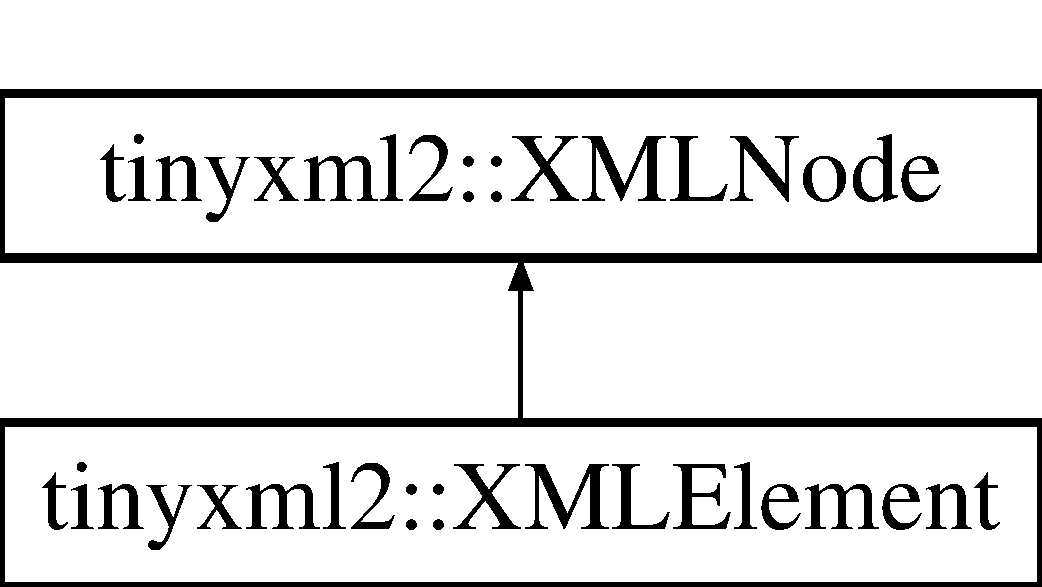
\includegraphics[height=2.000000cm]{classtinyxml2_1_1_x_m_l_element}
\end{center}
\end{figure}
\subsection*{Public Types}
\begin{DoxyCompactItemize}
\item 
enum \{ \hyperlink{classtinyxml2_1_1_x_m_l_element_a07a6ce25c17aaa505933db57f2373e50a78cf277c55b4655c86458dfecb11d349}{O\-P\-E\-N}, 
\hyperlink{classtinyxml2_1_1_x_m_l_element_a07a6ce25c17aaa505933db57f2373e50aa2f1f384020d2d4538ad2ec84930a028}{C\-L\-O\-S\-E\-D}, 
\hyperlink{classtinyxml2_1_1_x_m_l_element_a07a6ce25c17aaa505933db57f2373e50aa2857344b98a931536c443cd0cadc4b7}{C\-L\-O\-S\-I\-N\-G}
 \}
\end{DoxyCompactItemize}
\subsection*{Public Member Functions}
\begin{DoxyCompactItemize}
\item 
const char $\ast$ \hyperlink{classtinyxml2_1_1_x_m_l_element_a8bff355472bce2c60d4b50a212bf7f5f}{Name} () const 
\begin{DoxyCompactList}\small\item\em Get the name of an element (which is the \hyperlink{classtinyxml2_1_1_x_m_l_node_a7682be117e3b2b4ebfd517c1acaaadbf}{Value()} of the node.) \end{DoxyCompactList}\item 
void \hyperlink{classtinyxml2_1_1_x_m_l_element_a97712009a530d8cb8a63bf705f02b4f1}{Set\-Name} (const char $\ast$str, bool static\-Mem=false)
\begin{DoxyCompactList}\small\item\em Set the name of the element. \end{DoxyCompactList}\item 
virtual \hyperlink{classtinyxml2_1_1_x_m_l_element}{X\-M\-L\-Element} $\ast$ \hyperlink{classtinyxml2_1_1_x_m_l_element_ad9ff5c2dbc15df36cf664ce1b0ea0a5d}{To\-Element} ()
\begin{DoxyCompactList}\small\item\em Safely cast to an Element, or null. \end{DoxyCompactList}\item 
virtual const \hyperlink{classtinyxml2_1_1_x_m_l_element}{X\-M\-L\-Element} $\ast$ \hyperlink{classtinyxml2_1_1_x_m_l_element_a55acab615353ddabab48271f95816b0d}{To\-Element} () const 
\item 
virtual bool \hyperlink{classtinyxml2_1_1_x_m_l_element_a36d65438991a1e85096caf39ad13a099}{Accept} (\hyperlink{classtinyxml2_1_1_x_m_l_visitor}{X\-M\-L\-Visitor} $\ast$visitor) const 
\item 
const char $\ast$ \hyperlink{classtinyxml2_1_1_x_m_l_element_a7bdebdf1888074087237f3dd03912740}{Attribute} (const char $\ast$name, const char $\ast$value=0) const 
\item 
int \hyperlink{classtinyxml2_1_1_x_m_l_element_af86f05771c11a73a2896b662bb589ef5}{Int\-Attribute} (const char $\ast$name) const 
\item 
unsigned \hyperlink{classtinyxml2_1_1_x_m_l_element_aa5a41367b5118acec42a87f5f94cec2d}{Unsigned\-Attribute} (const char $\ast$name) const 
\begin{DoxyCompactList}\small\item\em See \hyperlink{classtinyxml2_1_1_x_m_l_element_af86f05771c11a73a2896b662bb589ef5}{Int\-Attribute()} \end{DoxyCompactList}\item 
bool \hyperlink{classtinyxml2_1_1_x_m_l_element_a34811e4d1881e4ecc95c49f0f3799115}{Bool\-Attribute} (const char $\ast$name) const 
\begin{DoxyCompactList}\small\item\em See \hyperlink{classtinyxml2_1_1_x_m_l_element_af86f05771c11a73a2896b662bb589ef5}{Int\-Attribute()} \end{DoxyCompactList}\item 
double \hyperlink{classtinyxml2_1_1_x_m_l_element_a536922a5cae9c9769a3dc1b7a8ff0d44}{Double\-Attribute} (const char $\ast$name) const 
\begin{DoxyCompactList}\small\item\em See \hyperlink{classtinyxml2_1_1_x_m_l_element_af86f05771c11a73a2896b662bb589ef5}{Int\-Attribute()} \end{DoxyCompactList}\item 
float \hyperlink{classtinyxml2_1_1_x_m_l_element_a33b69f123f995aff966d2e351bc51b1f}{Float\-Attribute} (const char $\ast$name) const 
\begin{DoxyCompactList}\small\item\em See \hyperlink{classtinyxml2_1_1_x_m_l_element_af86f05771c11a73a2896b662bb589ef5}{Int\-Attribute()} \end{DoxyCompactList}\item 
\hyperlink{namespacetinyxml2_a1fbf88509c3ac88c09117b1947414e08}{X\-M\-L\-Error} \hyperlink{classtinyxml2_1_1_x_m_l_element_a8b92c729346aa8ea9acd59ed3e9f2378}{Query\-Int\-Attribute} (const char $\ast$name, int $\ast$value) const 
\item 
\hyperlink{namespacetinyxml2_a1fbf88509c3ac88c09117b1947414e08}{X\-M\-L\-Error} \hyperlink{classtinyxml2_1_1_x_m_l_element_aa3d8d1b9311da8fc249b4352749aaa84}{Query\-Unsigned\-Attribute} (const char $\ast$name, unsigned int $\ast$value) const 
\begin{DoxyCompactList}\small\item\em See \hyperlink{classtinyxml2_1_1_x_m_l_element_a8b92c729346aa8ea9acd59ed3e9f2378}{Query\-Int\-Attribute()} \end{DoxyCompactList}\item 
\hyperlink{namespacetinyxml2_a1fbf88509c3ac88c09117b1947414e08}{X\-M\-L\-Error} \hyperlink{classtinyxml2_1_1_x_m_l_element_a2a58ee941c3cda23772c887a8f8b534e}{Query\-Bool\-Attribute} (const char $\ast$name, bool $\ast$value) const 
\begin{DoxyCompactList}\small\item\em See \hyperlink{classtinyxml2_1_1_x_m_l_element_a8b92c729346aa8ea9acd59ed3e9f2378}{Query\-Int\-Attribute()} \end{DoxyCompactList}\item 
\hyperlink{namespacetinyxml2_a1fbf88509c3ac88c09117b1947414e08}{X\-M\-L\-Error} \hyperlink{classtinyxml2_1_1_x_m_l_element_a1ffeed461d3e4020b39652cd6d3cd773}{Query\-Double\-Attribute} (const char $\ast$name, double $\ast$value) const 
\begin{DoxyCompactList}\small\item\em See \hyperlink{classtinyxml2_1_1_x_m_l_element_a8b92c729346aa8ea9acd59ed3e9f2378}{Query\-Int\-Attribute()} \end{DoxyCompactList}\item 
\hyperlink{namespacetinyxml2_a1fbf88509c3ac88c09117b1947414e08}{X\-M\-L\-Error} \hyperlink{classtinyxml2_1_1_x_m_l_element_a3f154e0b4b6903249ff9f758921758e5}{Query\-Float\-Attribute} (const char $\ast$name, float $\ast$value) const 
\begin{DoxyCompactList}\small\item\em See \hyperlink{classtinyxml2_1_1_x_m_l_element_a8b92c729346aa8ea9acd59ed3e9f2378}{Query\-Int\-Attribute()} \end{DoxyCompactList}\item 
int \hyperlink{classtinyxml2_1_1_x_m_l_element_aa471a199af9f137ef371f5db1ed1016b}{Query\-Attribute} (const char $\ast$name, int $\ast$value) const 
\item 
int \hyperlink{classtinyxml2_1_1_x_m_l_element_a60d18656aa70adb257eab18913aa4330}{Query\-Attribute} (const char $\ast$name, unsigned int $\ast$value) const 
\item 
int \hyperlink{classtinyxml2_1_1_x_m_l_element_a23fa8bac4250249c476c6bfdb6cb9b9c}{Query\-Attribute} (const char $\ast$name, bool $\ast$value) const 
\item 
int \hyperlink{classtinyxml2_1_1_x_m_l_element_a64aadcbf27423410e2896baf240f63f9}{Query\-Attribute} (const char $\ast$name, double $\ast$value) const 
\item 
int \hyperlink{classtinyxml2_1_1_x_m_l_element_afd553774be0e7760d73003058efa8df9}{Query\-Attribute} (const char $\ast$name, float $\ast$value) const 
\item 
void \hyperlink{classtinyxml2_1_1_x_m_l_element_a11943abf2d0831548c3790dd5d9f119c}{Set\-Attribute} (const char $\ast$name, const char $\ast$value)
\begin{DoxyCompactList}\small\item\em Sets the named attribute to value. \end{DoxyCompactList}\item 
void \hyperlink{classtinyxml2_1_1_x_m_l_element_aae6568c64c7f1cc88be8461ba41a79cf}{Set\-Attribute} (const char $\ast$name, int value)
\begin{DoxyCompactList}\small\item\em Sets the named attribute to value. \end{DoxyCompactList}\item 
void \hyperlink{classtinyxml2_1_1_x_m_l_element_ae143997e90064ba82326b29a9930ea8f}{Set\-Attribute} (const char $\ast$name, unsigned value)
\begin{DoxyCompactList}\small\item\em Sets the named attribute to value. \end{DoxyCompactList}\item 
void \hyperlink{classtinyxml2_1_1_x_m_l_element_aa848b696e6a75e4e545c6da9893b11e1}{Set\-Attribute} (const char $\ast$name, bool value)
\begin{DoxyCompactList}\small\item\em Sets the named attribute to value. \end{DoxyCompactList}\item 
void \hyperlink{classtinyxml2_1_1_x_m_l_element_a233397ee81e70eb5d4b814c5f8698533}{Set\-Attribute} (const char $\ast$name, double value)
\begin{DoxyCompactList}\small\item\em Sets the named attribute to value. \end{DoxyCompactList}\item 
void \hyperlink{classtinyxml2_1_1_x_m_l_element_aebd45aa7118964c30b32fe12e944628a}{Delete\-Attribute} (const char $\ast$name)
\item 
const \hyperlink{classtinyxml2_1_1_x_m_l_attribute}{X\-M\-L\-Attribute} $\ast$ \hyperlink{classtinyxml2_1_1_x_m_l_element_a67593e63558ffda0386699c3e4cc0b2c}{First\-Attribute} () const 
\begin{DoxyCompactList}\small\item\em Return the first attribute in the list. \end{DoxyCompactList}\item 
const \hyperlink{classtinyxml2_1_1_x_m_l_attribute}{X\-M\-L\-Attribute} $\ast$ \hyperlink{classtinyxml2_1_1_x_m_l_element_aaf46b0799ea419e5d070ac9a357de48f}{Find\-Attribute} (const char $\ast$name) const 
\begin{DoxyCompactList}\small\item\em Query a specific attribute in the list. \end{DoxyCompactList}\item 
const char $\ast$ \hyperlink{classtinyxml2_1_1_x_m_l_element_a56cc727044dad002b978256754d43a4b}{Get\-Text} () const 
\item 
\hyperlink{namespacetinyxml2_a1fbf88509c3ac88c09117b1947414e08}{X\-M\-L\-Error} \hyperlink{classtinyxml2_1_1_x_m_l_element_a71327c9a9d8840562bd204f46d0a7189}{Query\-Int\-Text} (int $\ast$ival) const 
\item 
\hyperlink{namespacetinyxml2_a1fbf88509c3ac88c09117b1947414e08}{X\-M\-L\-Error} \hyperlink{classtinyxml2_1_1_x_m_l_element_a2192091dec0c06be8b14f4e912c01758}{Query\-Unsigned\-Text} (unsigned $\ast$uval) const 
\begin{DoxyCompactList}\small\item\em See \hyperlink{classtinyxml2_1_1_x_m_l_element_a71327c9a9d8840562bd204f46d0a7189}{Query\-Int\-Text()} \end{DoxyCompactList}\item 
\hyperlink{namespacetinyxml2_a1fbf88509c3ac88c09117b1947414e08}{X\-M\-L\-Error} \hyperlink{classtinyxml2_1_1_x_m_l_element_afeb060672fa934163fc573e692b7fe38}{Query\-Bool\-Text} (bool $\ast$bval) const 
\begin{DoxyCompactList}\small\item\em See \hyperlink{classtinyxml2_1_1_x_m_l_element_a71327c9a9d8840562bd204f46d0a7189}{Query\-Int\-Text()} \end{DoxyCompactList}\item 
\hyperlink{namespacetinyxml2_a1fbf88509c3ac88c09117b1947414e08}{X\-M\-L\-Error} \hyperlink{classtinyxml2_1_1_x_m_l_element_aad931c42548907dbea416f7365d78b57}{Query\-Double\-Text} (double $\ast$dval) const 
\begin{DoxyCompactList}\small\item\em See \hyperlink{classtinyxml2_1_1_x_m_l_element_a71327c9a9d8840562bd204f46d0a7189}{Query\-Int\-Text()} \end{DoxyCompactList}\item 
\hyperlink{namespacetinyxml2_a1fbf88509c3ac88c09117b1947414e08}{X\-M\-L\-Error} \hyperlink{classtinyxml2_1_1_x_m_l_element_a11fa26e1dbca88e973964c1d9b597658}{Query\-Float\-Text} (float $\ast$fval) const 
\begin{DoxyCompactList}\small\item\em See \hyperlink{classtinyxml2_1_1_x_m_l_element_a71327c9a9d8840562bd204f46d0a7189}{Query\-Int\-Text()} \end{DoxyCompactList}\item 
int \hyperlink{classtinyxml2_1_1_x_m_l_element_a2e3d9f938307a05963d7c4b8cd55754e}{Closing\-Type} () const 
\item 
char $\ast$ \hyperlink{classtinyxml2_1_1_x_m_l_element_aaafdd2a5618abe80a2c1839ad3ccd492}{Parse\-Deep} (char $\ast$p, \hyperlink{classtinyxml2_1_1_str_pair}{Str\-Pair} $\ast$end\-Tag)
\item 
virtual \hyperlink{classtinyxml2_1_1_x_m_l_node}{X\-M\-L\-Node} $\ast$ \hyperlink{classtinyxml2_1_1_x_m_l_element_a85d85e32c18863fff1eeed53ae1ce23d}{Shallow\-Clone} (\hyperlink{classtinyxml2_1_1_x_m_l_document}{X\-M\-L\-Document} $\ast$document) const 
\item 
virtual bool \hyperlink{classtinyxml2_1_1_x_m_l_element_a25d51a2aad92625c78441457d58c85bc}{Shallow\-Equal} (const \hyperlink{classtinyxml2_1_1_x_m_l_node}{X\-M\-L\-Node} $\ast$compare) const 
\end{DoxyCompactItemize}
\subsection*{Friends}
\begin{DoxyCompactItemize}
\item 
class \hyperlink{classtinyxml2_1_1_x_m_l_element_a449202cfc89e7ae5c2f81995476f9ec1}{X\-M\-L\-Base}
\item 
class \hyperlink{classtinyxml2_1_1_x_m_l_element_a4eee3bda60c60a30e4e8cd4ea91c4c6e}{X\-M\-L\-Document}
\end{DoxyCompactItemize}
\subsection*{Additional Inherited Members}


\subsection{Detailed Description}
The element is a container class. It has a value, the element name, and can contain other elements, text, comments, and unknowns. Elements also contain an arbitrary number of attributes. 

Definition at line 1108 of file tinyxml2.\-hpp.



\subsection{Member Enumeration Documentation}
\hypertarget{classtinyxml2_1_1_x_m_l_element_a07a6ce25c17aaa505933db57f2373e50}{\subsubsection[{anonymous enum}]{\setlength{\rightskip}{0pt plus 5cm}anonymous enum}}\label{classtinyxml2_1_1_x_m_l_element_a07a6ce25c17aaa505933db57f2373e50}
\begin{Desc}
\item[Enumerator]\par
\begin{description}
\index{O\-P\-E\-N@{O\-P\-E\-N}!tinyxml2\-::\-X\-M\-L\-Element@{tinyxml2\-::\-X\-M\-L\-Element}}\index{tinyxml2\-::\-X\-M\-L\-Element@{tinyxml2\-::\-X\-M\-L\-Element}!O\-P\-E\-N@{O\-P\-E\-N}}\item[{\em 
\hypertarget{classtinyxml2_1_1_x_m_l_element_a07a6ce25c17aaa505933db57f2373e50a78cf277c55b4655c86458dfecb11d349}{O\-P\-E\-N}\label{classtinyxml2_1_1_x_m_l_element_a07a6ce25c17aaa505933db57f2373e50a78cf277c55b4655c86458dfecb11d349}
}]\index{C\-L\-O\-S\-E\-D@{C\-L\-O\-S\-E\-D}!tinyxml2\-::\-X\-M\-L\-Element@{tinyxml2\-::\-X\-M\-L\-Element}}\index{tinyxml2\-::\-X\-M\-L\-Element@{tinyxml2\-::\-X\-M\-L\-Element}!C\-L\-O\-S\-E\-D@{C\-L\-O\-S\-E\-D}}\item[{\em 
\hypertarget{classtinyxml2_1_1_x_m_l_element_a07a6ce25c17aaa505933db57f2373e50aa2f1f384020d2d4538ad2ec84930a028}{C\-L\-O\-S\-E\-D}\label{classtinyxml2_1_1_x_m_l_element_a07a6ce25c17aaa505933db57f2373e50aa2f1f384020d2d4538ad2ec84930a028}
}]\index{C\-L\-O\-S\-I\-N\-G@{C\-L\-O\-S\-I\-N\-G}!tinyxml2\-::\-X\-M\-L\-Element@{tinyxml2\-::\-X\-M\-L\-Element}}\index{tinyxml2\-::\-X\-M\-L\-Element@{tinyxml2\-::\-X\-M\-L\-Element}!C\-L\-O\-S\-I\-N\-G@{C\-L\-O\-S\-I\-N\-G}}\item[{\em 
\hypertarget{classtinyxml2_1_1_x_m_l_element_a07a6ce25c17aaa505933db57f2373e50aa2857344b98a931536c443cd0cadc4b7}{C\-L\-O\-S\-I\-N\-G}\label{classtinyxml2_1_1_x_m_l_element_a07a6ce25c17aaa505933db57f2373e50aa2857344b98a931536c443cd0cadc4b7}
}]\end{description}
\end{Desc}


Definition at line 1386 of file tinyxml2.\-hpp.



\subsection{Member Function Documentation}
\hypertarget{classtinyxml2_1_1_x_m_l_element_a36d65438991a1e85096caf39ad13a099}{\index{tinyxml2\-::\-X\-M\-L\-Element@{tinyxml2\-::\-X\-M\-L\-Element}!Accept@{Accept}}
\index{Accept@{Accept}!tinyxml2::XMLElement@{tinyxml2\-::\-X\-M\-L\-Element}}
\subsubsection[{Accept}]{\setlength{\rightskip}{0pt plus 5cm}bool tinyxml2\-::\-X\-M\-L\-Element\-::\-Accept (
\begin{DoxyParamCaption}
\item[{{\bf X\-M\-L\-Visitor} $\ast$}]{visitor}
\end{DoxyParamCaption}
) const\hspace{0.3cm}{\ttfamily [virtual]}}}\label{classtinyxml2_1_1_x_m_l_element_a36d65438991a1e85096caf39ad13a099}
Accept a hierarchical visit of the nodes in the Tiny\-X\-M\-L-\/2 D\-O\-M. Every node in the X\-M\-L tree will be conditionally visited and the host will be called back via the \hyperlink{classtinyxml2_1_1_x_m_l_visitor}{X\-M\-L\-Visitor} interface.

This is essentially a S\-A\-X interface for Tiny\-X\-M\-L-\/2. (Note however it doesn't re-\/parse the X\-M\-L for the callbacks, so the performance of Tiny\-X\-M\-L-\/2 is unchanged by using this interface versus any other.)

The interface has been based on ideas from\-:


\begin{DoxyItemize}
\item \href{http://www.saxproject.org/}{\tt http\-://www.\-saxproject.\-org/}
\item \href{http://c2.com/cgi/wiki?HierarchicalVisitorPattern}{\tt http\-://c2.\-com/cgi/wiki?\-Hierarchical\-Visitor\-Pattern}
\end{DoxyItemize}

Which are both good references for \char`\"{}visiting\char`\"{}.

An example of using \hyperlink{classtinyxml2_1_1_x_m_l_element_a36d65438991a1e85096caf39ad13a099}{Accept()}\-: \begin{DoxyVerb}XMLPrinter printer;
tinyxmlDoc.Accept( &printer );
const char* xmlcstr = printer.CStr();
\end{DoxyVerb}
 

Implements \hyperlink{classtinyxml2_1_1_x_m_l_node_a81e66df0a44c67a7af17f3b77a152785}{tinyxml2\-::\-X\-M\-L\-Node}.



Definition at line 1473 of file tinyxml2.\-cpp.

\hypertarget{classtinyxml2_1_1_x_m_l_element_a7bdebdf1888074087237f3dd03912740}{\index{tinyxml2\-::\-X\-M\-L\-Element@{tinyxml2\-::\-X\-M\-L\-Element}!Attribute@{Attribute}}
\index{Attribute@{Attribute}!tinyxml2::XMLElement@{tinyxml2\-::\-X\-M\-L\-Element}}
\subsubsection[{Attribute}]{\setlength{\rightskip}{0pt plus 5cm}const char $\ast$ tinyxml2\-::\-X\-M\-L\-Element\-::\-Attribute (
\begin{DoxyParamCaption}
\item[{const char $\ast$}]{name, }
\item[{const char $\ast$}]{value = {\ttfamily 0}}
\end{DoxyParamCaption}
) const}}\label{classtinyxml2_1_1_x_m_l_element_a7bdebdf1888074087237f3dd03912740}
Given an attribute name, \hyperlink{classtinyxml2_1_1_x_m_l_element_a7bdebdf1888074087237f3dd03912740}{Attribute()} returns the value for the attribute of that name, or null if none exists. For example\-:

\begin{DoxyVerb}const char* value = ele->Attribute( "foo" );
\end{DoxyVerb}


The 'value' parameter is normally null. However, if specified, the attribute will only be returned if the 'name' and 'value' match. This allow you to write code\-:

\begin{DoxyVerb}if ( ele->Attribute( "foo", "bar" ) ) callFooIsBar();
\end{DoxyVerb}


rather than\-: \begin{DoxyVerb}if ( ele->Attribute( "foo" ) ) {
    if ( strcmp( ele->Attribute( "foo" ), "bar" ) == 0 ) callFooIsBar();
}
\end{DoxyVerb}
 

Definition at line 1208 of file tinyxml2.\-cpp.

\hypertarget{classtinyxml2_1_1_x_m_l_element_a34811e4d1881e4ecc95c49f0f3799115}{\index{tinyxml2\-::\-X\-M\-L\-Element@{tinyxml2\-::\-X\-M\-L\-Element}!Bool\-Attribute@{Bool\-Attribute}}
\index{Bool\-Attribute@{Bool\-Attribute}!tinyxml2::XMLElement@{tinyxml2\-::\-X\-M\-L\-Element}}
\subsubsection[{Bool\-Attribute}]{\setlength{\rightskip}{0pt plus 5cm}bool tinyxml2\-::\-X\-M\-L\-Element\-::\-Bool\-Attribute (
\begin{DoxyParamCaption}
\item[{const char $\ast$}]{name}
\end{DoxyParamCaption}
) const\hspace{0.3cm}{\ttfamily [inline]}}}\label{classtinyxml2_1_1_x_m_l_element_a34811e4d1881e4ecc95c49f0f3799115}


See \hyperlink{classtinyxml2_1_1_x_m_l_element_af86f05771c11a73a2896b662bb589ef5}{Int\-Attribute()} 



Definition at line 1172 of file tinyxml2.\-hpp.

\hypertarget{classtinyxml2_1_1_x_m_l_element_a2e3d9f938307a05963d7c4b8cd55754e}{\index{tinyxml2\-::\-X\-M\-L\-Element@{tinyxml2\-::\-X\-M\-L\-Element}!Closing\-Type@{Closing\-Type}}
\index{Closing\-Type@{Closing\-Type}!tinyxml2::XMLElement@{tinyxml2\-::\-X\-M\-L\-Element}}
\subsubsection[{Closing\-Type}]{\setlength{\rightskip}{0pt plus 5cm}int tinyxml2\-::\-X\-M\-L\-Element\-::\-Closing\-Type (
\begin{DoxyParamCaption}
{}
\end{DoxyParamCaption}
) const\hspace{0.3cm}{\ttfamily [inline]}}}\label{classtinyxml2_1_1_x_m_l_element_a2e3d9f938307a05963d7c4b8cd55754e}


Definition at line 1391 of file tinyxml2.\-hpp.

\hypertarget{classtinyxml2_1_1_x_m_l_element_aebd45aa7118964c30b32fe12e944628a}{\index{tinyxml2\-::\-X\-M\-L\-Element@{tinyxml2\-::\-X\-M\-L\-Element}!Delete\-Attribute@{Delete\-Attribute}}
\index{Delete\-Attribute@{Delete\-Attribute}!tinyxml2::XMLElement@{tinyxml2\-::\-X\-M\-L\-Element}}
\subsubsection[{Delete\-Attribute}]{\setlength{\rightskip}{0pt plus 5cm}void tinyxml2\-::\-X\-M\-L\-Element\-::\-Delete\-Attribute (
\begin{DoxyParamCaption}
\item[{const char $\ast$}]{name}
\end{DoxyParamCaption}
)}}\label{classtinyxml2_1_1_x_m_l_element_aebd45aa7118964c30b32fe12e944628a}
Delete an attribute. 

Definition at line 1323 of file tinyxml2.\-cpp.

\hypertarget{classtinyxml2_1_1_x_m_l_element_a536922a5cae9c9769a3dc1b7a8ff0d44}{\index{tinyxml2\-::\-X\-M\-L\-Element@{tinyxml2\-::\-X\-M\-L\-Element}!Double\-Attribute@{Double\-Attribute}}
\index{Double\-Attribute@{Double\-Attribute}!tinyxml2::XMLElement@{tinyxml2\-::\-X\-M\-L\-Element}}
\subsubsection[{Double\-Attribute}]{\setlength{\rightskip}{0pt plus 5cm}double tinyxml2\-::\-X\-M\-L\-Element\-::\-Double\-Attribute (
\begin{DoxyParamCaption}
\item[{const char $\ast$}]{name}
\end{DoxyParamCaption}
) const\hspace{0.3cm}{\ttfamily [inline]}}}\label{classtinyxml2_1_1_x_m_l_element_a536922a5cae9c9769a3dc1b7a8ff0d44}


See \hyperlink{classtinyxml2_1_1_x_m_l_element_af86f05771c11a73a2896b662bb589ef5}{Int\-Attribute()} 



Definition at line 1178 of file tinyxml2.\-hpp.

\hypertarget{classtinyxml2_1_1_x_m_l_element_aaf46b0799ea419e5d070ac9a357de48f}{\index{tinyxml2\-::\-X\-M\-L\-Element@{tinyxml2\-::\-X\-M\-L\-Element}!Find\-Attribute@{Find\-Attribute}}
\index{Find\-Attribute@{Find\-Attribute}!tinyxml2::XMLElement@{tinyxml2\-::\-X\-M\-L\-Element}}
\subsubsection[{Find\-Attribute}]{\setlength{\rightskip}{0pt plus 5cm}const {\bf X\-M\-L\-Attribute} $\ast$ tinyxml2\-::\-X\-M\-L\-Element\-::\-Find\-Attribute (
\begin{DoxyParamCaption}
\item[{const char $\ast$}]{name}
\end{DoxyParamCaption}
) const}}\label{classtinyxml2_1_1_x_m_l_element_aaf46b0799ea419e5d070ac9a357de48f}


Query a specific attribute in the list. 



Definition at line 1196 of file tinyxml2.\-cpp.

\hypertarget{classtinyxml2_1_1_x_m_l_element_a67593e63558ffda0386699c3e4cc0b2c}{\index{tinyxml2\-::\-X\-M\-L\-Element@{tinyxml2\-::\-X\-M\-L\-Element}!First\-Attribute@{First\-Attribute}}
\index{First\-Attribute@{First\-Attribute}!tinyxml2::XMLElement@{tinyxml2\-::\-X\-M\-L\-Element}}
\subsubsection[{First\-Attribute}]{\setlength{\rightskip}{0pt plus 5cm}const {\bf X\-M\-L\-Attribute}$\ast$ tinyxml2\-::\-X\-M\-L\-Element\-::\-First\-Attribute (
\begin{DoxyParamCaption}
{}
\end{DoxyParamCaption}
) const\hspace{0.3cm}{\ttfamily [inline]}}}\label{classtinyxml2_1_1_x_m_l_element_a67593e63558ffda0386699c3e4cc0b2c}


Return the first attribute in the list. 



Definition at line 1313 of file tinyxml2.\-hpp.

\hypertarget{classtinyxml2_1_1_x_m_l_element_a33b69f123f995aff966d2e351bc51b1f}{\index{tinyxml2\-::\-X\-M\-L\-Element@{tinyxml2\-::\-X\-M\-L\-Element}!Float\-Attribute@{Float\-Attribute}}
\index{Float\-Attribute@{Float\-Attribute}!tinyxml2::XMLElement@{tinyxml2\-::\-X\-M\-L\-Element}}
\subsubsection[{Float\-Attribute}]{\setlength{\rightskip}{0pt plus 5cm}float tinyxml2\-::\-X\-M\-L\-Element\-::\-Float\-Attribute (
\begin{DoxyParamCaption}
\item[{const char $\ast$}]{name}
\end{DoxyParamCaption}
) const\hspace{0.3cm}{\ttfamily [inline]}}}\label{classtinyxml2_1_1_x_m_l_element_a33b69f123f995aff966d2e351bc51b1f}


See \hyperlink{classtinyxml2_1_1_x_m_l_element_af86f05771c11a73a2896b662bb589ef5}{Int\-Attribute()} 



Definition at line 1184 of file tinyxml2.\-hpp.

\hypertarget{classtinyxml2_1_1_x_m_l_element_a56cc727044dad002b978256754d43a4b}{\index{tinyxml2\-::\-X\-M\-L\-Element@{tinyxml2\-::\-X\-M\-L\-Element}!Get\-Text@{Get\-Text}}
\index{Get\-Text@{Get\-Text}!tinyxml2::XMLElement@{tinyxml2\-::\-X\-M\-L\-Element}}
\subsubsection[{Get\-Text}]{\setlength{\rightskip}{0pt plus 5cm}const char $\ast$ tinyxml2\-::\-X\-M\-L\-Element\-::\-Get\-Text (
\begin{DoxyParamCaption}
{}
\end{DoxyParamCaption}
) const}}\label{classtinyxml2_1_1_x_m_l_element_a56cc727044dad002b978256754d43a4b}
Convenience function for easy access to the text inside an element. Although easy and concise, \hyperlink{classtinyxml2_1_1_x_m_l_element_a56cc727044dad002b978256754d43a4b}{Get\-Text()} is limited compared to getting the \hyperlink{classtinyxml2_1_1_x_m_l_text}{X\-M\-L\-Text} child and accessing it directly.

If the first child of 'this' is a \hyperlink{classtinyxml2_1_1_x_m_l_text}{X\-M\-L\-Text}, the \hyperlink{classtinyxml2_1_1_x_m_l_element_a56cc727044dad002b978256754d43a4b}{Get\-Text()} returns the character string of the Text node, else null is returned.

This is a convenient method for getting the text of simple contained text\-: \begin{DoxyVerb}<foo>This is text</foo>
    const char* str = fooElement->GetText();
\end{DoxyVerb}


'str' will be a pointer to \char`\"{}\-This is text\char`\"{}.

Note that this function can be misleading. If the element foo was created from this X\-M\-L\-: \begin{DoxyVerb}    <foo><b>This is text</b></foo>
\end{DoxyVerb}


then the value of str would be null. The first child node isn't a text node, it is another element. From this X\-M\-L\-: \begin{DoxyVerb}    <foo>This is <b>text</b></foo>
\end{DoxyVerb}
 \hyperlink{classtinyxml2_1_1_x_m_l_element_a56cc727044dad002b978256754d43a4b}{Get\-Text()} will return \char`\"{}\-This is \char`\"{}. 

Definition at line 1221 of file tinyxml2.\-cpp.

\hypertarget{classtinyxml2_1_1_x_m_l_element_af86f05771c11a73a2896b662bb589ef5}{\index{tinyxml2\-::\-X\-M\-L\-Element@{tinyxml2\-::\-X\-M\-L\-Element}!Int\-Attribute@{Int\-Attribute}}
\index{Int\-Attribute@{Int\-Attribute}!tinyxml2::XMLElement@{tinyxml2\-::\-X\-M\-L\-Element}}
\subsubsection[{Int\-Attribute}]{\setlength{\rightskip}{0pt plus 5cm}int tinyxml2\-::\-X\-M\-L\-Element\-::\-Int\-Attribute (
\begin{DoxyParamCaption}
\item[{const char $\ast$}]{name}
\end{DoxyParamCaption}
) const\hspace{0.3cm}{\ttfamily [inline]}}}\label{classtinyxml2_1_1_x_m_l_element_af86f05771c11a73a2896b662bb589ef5}
Given an attribute name, \hyperlink{classtinyxml2_1_1_x_m_l_element_af86f05771c11a73a2896b662bb589ef5}{Int\-Attribute()} returns the value of the attribute interpreted as an integer. 0 will be returned if there is an error. For a method with error checking, see \hyperlink{classtinyxml2_1_1_x_m_l_element_a8b92c729346aa8ea9acd59ed3e9f2378}{Query\-Int\-Attribute()} 

Definition at line 1160 of file tinyxml2.\-hpp.

\hypertarget{classtinyxml2_1_1_x_m_l_element_a8bff355472bce2c60d4b50a212bf7f5f}{\index{tinyxml2\-::\-X\-M\-L\-Element@{tinyxml2\-::\-X\-M\-L\-Element}!Name@{Name}}
\index{Name@{Name}!tinyxml2::XMLElement@{tinyxml2\-::\-X\-M\-L\-Element}}
\subsubsection[{Name}]{\setlength{\rightskip}{0pt plus 5cm}const char$\ast$ tinyxml2\-::\-X\-M\-L\-Element\-::\-Name (
\begin{DoxyParamCaption}
{}
\end{DoxyParamCaption}
) const\hspace{0.3cm}{\ttfamily [inline]}}}\label{classtinyxml2_1_1_x_m_l_element_a8bff355472bce2c60d4b50a212bf7f5f}


Get the name of an element (which is the \hyperlink{classtinyxml2_1_1_x_m_l_node_a7682be117e3b2b4ebfd517c1acaaadbf}{Value()} of the node.) 



Definition at line 1114 of file tinyxml2.\-hpp.

\hypertarget{classtinyxml2_1_1_x_m_l_element_aaafdd2a5618abe80a2c1839ad3ccd492}{\index{tinyxml2\-::\-X\-M\-L\-Element@{tinyxml2\-::\-X\-M\-L\-Element}!Parse\-Deep@{Parse\-Deep}}
\index{Parse\-Deep@{Parse\-Deep}!tinyxml2::XMLElement@{tinyxml2\-::\-X\-M\-L\-Element}}
\subsubsection[{Parse\-Deep}]{\setlength{\rightskip}{0pt plus 5cm}char $\ast$ tinyxml2\-::\-X\-M\-L\-Element\-::\-Parse\-Deep (
\begin{DoxyParamCaption}
\item[{char $\ast$}]{p, }
\item[{{\bf Str\-Pair} $\ast$}]{end\-Tag}
\end{DoxyParamCaption}
)\hspace{0.3cm}{\ttfamily [virtual]}}}\label{classtinyxml2_1_1_x_m_l_element_aaafdd2a5618abe80a2c1839ad3ccd492}


Reimplemented from \hyperlink{classtinyxml2_1_1_x_m_l_node_a7610d0f603e8b603d2078521811a23c1}{tinyxml2\-::\-X\-M\-L\-Node}.



Definition at line 1403 of file tinyxml2.\-cpp.

\hypertarget{classtinyxml2_1_1_x_m_l_element_aa471a199af9f137ef371f5db1ed1016b}{\index{tinyxml2\-::\-X\-M\-L\-Element@{tinyxml2\-::\-X\-M\-L\-Element}!Query\-Attribute@{Query\-Attribute}}
\index{Query\-Attribute@{Query\-Attribute}!tinyxml2::XMLElement@{tinyxml2\-::\-X\-M\-L\-Element}}
\subsubsection[{Query\-Attribute}]{\setlength{\rightskip}{0pt plus 5cm}int tinyxml2\-::\-X\-M\-L\-Element\-::\-Query\-Attribute (
\begin{DoxyParamCaption}
\item[{const char $\ast$}]{name, }
\item[{int $\ast$}]{value}
\end{DoxyParamCaption}
) const\hspace{0.3cm}{\ttfamily [inline]}}}\label{classtinyxml2_1_1_x_m_l_element_aa471a199af9f137ef371f5db1ed1016b}
Given an attribute name, \hyperlink{classtinyxml2_1_1_x_m_l_element_aa471a199af9f137ef371f5db1ed1016b}{Query\-Attribute()} returns X\-M\-L\-\_\-\-N\-O\-\_\-\-E\-R\-R\-O\-R, X\-M\-L\-\_\-\-W\-R\-O\-N\-G\-\_\-\-A\-T\-T\-R\-I\-B\-U\-T\-E\-\_\-\-T\-Y\-P\-E if the conversion can't be performed, or X\-M\-L\-\_\-\-N\-O\-\_\-\-A\-T\-T\-R\-I\-B\-U\-T\-E if the attribute doesn't exist. It is overloaded for the primitive types, and is a generally more convenient replacement of \hyperlink{classtinyxml2_1_1_x_m_l_element_a8b92c729346aa8ea9acd59ed3e9f2378}{Query\-Int\-Attribute()} and related functions.

If successful, the result of the conversion will be written to 'value'. If not successful, nothing will be written to 'value'. This allows you to provide default value\-:

\begin{DoxyVerb}int value = 10;
QueryAttribute( "foo", &value );        // if "foo" isn't found, value will still be 10
\end{DoxyVerb}
 

Definition at line 1261 of file tinyxml2.\-hpp.

\hypertarget{classtinyxml2_1_1_x_m_l_element_a60d18656aa70adb257eab18913aa4330}{\index{tinyxml2\-::\-X\-M\-L\-Element@{tinyxml2\-::\-X\-M\-L\-Element}!Query\-Attribute@{Query\-Attribute}}
\index{Query\-Attribute@{Query\-Attribute}!tinyxml2::XMLElement@{tinyxml2\-::\-X\-M\-L\-Element}}
\subsubsection[{Query\-Attribute}]{\setlength{\rightskip}{0pt plus 5cm}int tinyxml2\-::\-X\-M\-L\-Element\-::\-Query\-Attribute (
\begin{DoxyParamCaption}
\item[{const char $\ast$}]{name, }
\item[{unsigned int $\ast$}]{value}
\end{DoxyParamCaption}
) const\hspace{0.3cm}{\ttfamily [inline]}}}\label{classtinyxml2_1_1_x_m_l_element_a60d18656aa70adb257eab18913aa4330}


Definition at line 1265 of file tinyxml2.\-hpp.

\hypertarget{classtinyxml2_1_1_x_m_l_element_a23fa8bac4250249c476c6bfdb6cb9b9c}{\index{tinyxml2\-::\-X\-M\-L\-Element@{tinyxml2\-::\-X\-M\-L\-Element}!Query\-Attribute@{Query\-Attribute}}
\index{Query\-Attribute@{Query\-Attribute}!tinyxml2::XMLElement@{tinyxml2\-::\-X\-M\-L\-Element}}
\subsubsection[{Query\-Attribute}]{\setlength{\rightskip}{0pt plus 5cm}int tinyxml2\-::\-X\-M\-L\-Element\-::\-Query\-Attribute (
\begin{DoxyParamCaption}
\item[{const char $\ast$}]{name, }
\item[{bool $\ast$}]{value}
\end{DoxyParamCaption}
) const\hspace{0.3cm}{\ttfamily [inline]}}}\label{classtinyxml2_1_1_x_m_l_element_a23fa8bac4250249c476c6bfdb6cb9b9c}


Definition at line 1269 of file tinyxml2.\-hpp.

\hypertarget{classtinyxml2_1_1_x_m_l_element_a64aadcbf27423410e2896baf240f63f9}{\index{tinyxml2\-::\-X\-M\-L\-Element@{tinyxml2\-::\-X\-M\-L\-Element}!Query\-Attribute@{Query\-Attribute}}
\index{Query\-Attribute@{Query\-Attribute}!tinyxml2::XMLElement@{tinyxml2\-::\-X\-M\-L\-Element}}
\subsubsection[{Query\-Attribute}]{\setlength{\rightskip}{0pt plus 5cm}int tinyxml2\-::\-X\-M\-L\-Element\-::\-Query\-Attribute (
\begin{DoxyParamCaption}
\item[{const char $\ast$}]{name, }
\item[{double $\ast$}]{value}
\end{DoxyParamCaption}
) const\hspace{0.3cm}{\ttfamily [inline]}}}\label{classtinyxml2_1_1_x_m_l_element_a64aadcbf27423410e2896baf240f63f9}


Definition at line 1273 of file tinyxml2.\-hpp.

\hypertarget{classtinyxml2_1_1_x_m_l_element_afd553774be0e7760d73003058efa8df9}{\index{tinyxml2\-::\-X\-M\-L\-Element@{tinyxml2\-::\-X\-M\-L\-Element}!Query\-Attribute@{Query\-Attribute}}
\index{Query\-Attribute@{Query\-Attribute}!tinyxml2::XMLElement@{tinyxml2\-::\-X\-M\-L\-Element}}
\subsubsection[{Query\-Attribute}]{\setlength{\rightskip}{0pt plus 5cm}int tinyxml2\-::\-X\-M\-L\-Element\-::\-Query\-Attribute (
\begin{DoxyParamCaption}
\item[{const char $\ast$}]{name, }
\item[{float $\ast$}]{value}
\end{DoxyParamCaption}
) const\hspace{0.3cm}{\ttfamily [inline]}}}\label{classtinyxml2_1_1_x_m_l_element_afd553774be0e7760d73003058efa8df9}


Definition at line 1277 of file tinyxml2.\-hpp.

\hypertarget{classtinyxml2_1_1_x_m_l_element_a2a58ee941c3cda23772c887a8f8b534e}{\index{tinyxml2\-::\-X\-M\-L\-Element@{tinyxml2\-::\-X\-M\-L\-Element}!Query\-Bool\-Attribute@{Query\-Bool\-Attribute}}
\index{Query\-Bool\-Attribute@{Query\-Bool\-Attribute}!tinyxml2::XMLElement@{tinyxml2\-::\-X\-M\-L\-Element}}
\subsubsection[{Query\-Bool\-Attribute}]{\setlength{\rightskip}{0pt plus 5cm}{\bf X\-M\-L\-Error} tinyxml2\-::\-X\-M\-L\-Element\-::\-Query\-Bool\-Attribute (
\begin{DoxyParamCaption}
\item[{const char $\ast$}]{name, }
\item[{bool $\ast$}]{value}
\end{DoxyParamCaption}
) const\hspace{0.3cm}{\ttfamily [inline]}}}\label{classtinyxml2_1_1_x_m_l_element_a2a58ee941c3cda23772c887a8f8b534e}


See \hyperlink{classtinyxml2_1_1_x_m_l_element_a8b92c729346aa8ea9acd59ed3e9f2378}{Query\-Int\-Attribute()} 



Definition at line 1219 of file tinyxml2.\-hpp.

\hypertarget{classtinyxml2_1_1_x_m_l_element_afeb060672fa934163fc573e692b7fe38}{\index{tinyxml2\-::\-X\-M\-L\-Element@{tinyxml2\-::\-X\-M\-L\-Element}!Query\-Bool\-Text@{Query\-Bool\-Text}}
\index{Query\-Bool\-Text@{Query\-Bool\-Text}!tinyxml2::XMLElement@{tinyxml2\-::\-X\-M\-L\-Element}}
\subsubsection[{Query\-Bool\-Text}]{\setlength{\rightskip}{0pt plus 5cm}{\bf X\-M\-L\-Error} tinyxml2\-::\-X\-M\-L\-Element\-::\-Query\-Bool\-Text (
\begin{DoxyParamCaption}
\item[{bool $\ast$}]{bval}
\end{DoxyParamCaption}
) const}}\label{classtinyxml2_1_1_x_m_l_element_afeb060672fa934163fc573e692b7fe38}


See \hyperlink{classtinyxml2_1_1_x_m_l_element_a71327c9a9d8840562bd204f46d0a7189}{Query\-Int\-Text()} 



Definition at line 1256 of file tinyxml2.\-cpp.

\hypertarget{classtinyxml2_1_1_x_m_l_element_a1ffeed461d3e4020b39652cd6d3cd773}{\index{tinyxml2\-::\-X\-M\-L\-Element@{tinyxml2\-::\-X\-M\-L\-Element}!Query\-Double\-Attribute@{Query\-Double\-Attribute}}
\index{Query\-Double\-Attribute@{Query\-Double\-Attribute}!tinyxml2::XMLElement@{tinyxml2\-::\-X\-M\-L\-Element}}
\subsubsection[{Query\-Double\-Attribute}]{\setlength{\rightskip}{0pt plus 5cm}{\bf X\-M\-L\-Error} tinyxml2\-::\-X\-M\-L\-Element\-::\-Query\-Double\-Attribute (
\begin{DoxyParamCaption}
\item[{const char $\ast$}]{name, }
\item[{double $\ast$}]{value}
\end{DoxyParamCaption}
) const\hspace{0.3cm}{\ttfamily [inline]}}}\label{classtinyxml2_1_1_x_m_l_element_a1ffeed461d3e4020b39652cd6d3cd773}


See \hyperlink{classtinyxml2_1_1_x_m_l_element_a8b92c729346aa8ea9acd59ed3e9f2378}{Query\-Int\-Attribute()} 



Definition at line 1227 of file tinyxml2.\-hpp.

\hypertarget{classtinyxml2_1_1_x_m_l_element_aad931c42548907dbea416f7365d78b57}{\index{tinyxml2\-::\-X\-M\-L\-Element@{tinyxml2\-::\-X\-M\-L\-Element}!Query\-Double\-Text@{Query\-Double\-Text}}
\index{Query\-Double\-Text@{Query\-Double\-Text}!tinyxml2::XMLElement@{tinyxml2\-::\-X\-M\-L\-Element}}
\subsubsection[{Query\-Double\-Text}]{\setlength{\rightskip}{0pt plus 5cm}{\bf X\-M\-L\-Error} tinyxml2\-::\-X\-M\-L\-Element\-::\-Query\-Double\-Text (
\begin{DoxyParamCaption}
\item[{double $\ast$}]{dval}
\end{DoxyParamCaption}
) const}}\label{classtinyxml2_1_1_x_m_l_element_aad931c42548907dbea416f7365d78b57}


See \hyperlink{classtinyxml2_1_1_x_m_l_element_a71327c9a9d8840562bd204f46d0a7189}{Query\-Int\-Text()} 



Definition at line 1269 of file tinyxml2.\-cpp.

\hypertarget{classtinyxml2_1_1_x_m_l_element_a3f154e0b4b6903249ff9f758921758e5}{\index{tinyxml2\-::\-X\-M\-L\-Element@{tinyxml2\-::\-X\-M\-L\-Element}!Query\-Float\-Attribute@{Query\-Float\-Attribute}}
\index{Query\-Float\-Attribute@{Query\-Float\-Attribute}!tinyxml2::XMLElement@{tinyxml2\-::\-X\-M\-L\-Element}}
\subsubsection[{Query\-Float\-Attribute}]{\setlength{\rightskip}{0pt plus 5cm}{\bf X\-M\-L\-Error} tinyxml2\-::\-X\-M\-L\-Element\-::\-Query\-Float\-Attribute (
\begin{DoxyParamCaption}
\item[{const char $\ast$}]{name, }
\item[{float $\ast$}]{value}
\end{DoxyParamCaption}
) const\hspace{0.3cm}{\ttfamily [inline]}}}\label{classtinyxml2_1_1_x_m_l_element_a3f154e0b4b6903249ff9f758921758e5}


See \hyperlink{classtinyxml2_1_1_x_m_l_element_a8b92c729346aa8ea9acd59ed3e9f2378}{Query\-Int\-Attribute()} 



Definition at line 1235 of file tinyxml2.\-hpp.

\hypertarget{classtinyxml2_1_1_x_m_l_element_a11fa26e1dbca88e973964c1d9b597658}{\index{tinyxml2\-::\-X\-M\-L\-Element@{tinyxml2\-::\-X\-M\-L\-Element}!Query\-Float\-Text@{Query\-Float\-Text}}
\index{Query\-Float\-Text@{Query\-Float\-Text}!tinyxml2::XMLElement@{tinyxml2\-::\-X\-M\-L\-Element}}
\subsubsection[{Query\-Float\-Text}]{\setlength{\rightskip}{0pt plus 5cm}{\bf X\-M\-L\-Error} tinyxml2\-::\-X\-M\-L\-Element\-::\-Query\-Float\-Text (
\begin{DoxyParamCaption}
\item[{float $\ast$}]{fval}
\end{DoxyParamCaption}
) const}}\label{classtinyxml2_1_1_x_m_l_element_a11fa26e1dbca88e973964c1d9b597658}


See \hyperlink{classtinyxml2_1_1_x_m_l_element_a71327c9a9d8840562bd204f46d0a7189}{Query\-Int\-Text()} 



Definition at line 1282 of file tinyxml2.\-cpp.

\hypertarget{classtinyxml2_1_1_x_m_l_element_a8b92c729346aa8ea9acd59ed3e9f2378}{\index{tinyxml2\-::\-X\-M\-L\-Element@{tinyxml2\-::\-X\-M\-L\-Element}!Query\-Int\-Attribute@{Query\-Int\-Attribute}}
\index{Query\-Int\-Attribute@{Query\-Int\-Attribute}!tinyxml2::XMLElement@{tinyxml2\-::\-X\-M\-L\-Element}}
\subsubsection[{Query\-Int\-Attribute}]{\setlength{\rightskip}{0pt plus 5cm}{\bf X\-M\-L\-Error} tinyxml2\-::\-X\-M\-L\-Element\-::\-Query\-Int\-Attribute (
\begin{DoxyParamCaption}
\item[{const char $\ast$}]{name, }
\item[{int $\ast$}]{value}
\end{DoxyParamCaption}
) const\hspace{0.3cm}{\ttfamily [inline]}}}\label{classtinyxml2_1_1_x_m_l_element_a8b92c729346aa8ea9acd59ed3e9f2378}
Given an attribute name, \hyperlink{classtinyxml2_1_1_x_m_l_element_a8b92c729346aa8ea9acd59ed3e9f2378}{Query\-Int\-Attribute()} returns X\-M\-L\-\_\-\-N\-O\-\_\-\-E\-R\-R\-O\-R, X\-M\-L\-\_\-\-W\-R\-O\-N\-G\-\_\-\-A\-T\-T\-R\-I\-B\-U\-T\-E\-\_\-\-T\-Y\-P\-E if the conversion can't be performed, or X\-M\-L\-\_\-\-N\-O\-\_\-\-A\-T\-T\-R\-I\-B\-U\-T\-E if the attribute doesn't exist. If successful, the result of the conversion will be written to 'value'. If not successful, nothing will be written to 'value'. This allows you to provide default value\-:

\begin{DoxyVerb}int value = 10;
QueryIntAttribute( "foo", &value );     // if "foo" isn't found, value will still be 10
\end{DoxyVerb}
 

Definition at line 1203 of file tinyxml2.\-hpp.

\hypertarget{classtinyxml2_1_1_x_m_l_element_a71327c9a9d8840562bd204f46d0a7189}{\index{tinyxml2\-::\-X\-M\-L\-Element@{tinyxml2\-::\-X\-M\-L\-Element}!Query\-Int\-Text@{Query\-Int\-Text}}
\index{Query\-Int\-Text@{Query\-Int\-Text}!tinyxml2::XMLElement@{tinyxml2\-::\-X\-M\-L\-Element}}
\subsubsection[{Query\-Int\-Text}]{\setlength{\rightskip}{0pt plus 5cm}{\bf X\-M\-L\-Error} tinyxml2\-::\-X\-M\-L\-Element\-::\-Query\-Int\-Text (
\begin{DoxyParamCaption}
\item[{int $\ast$}]{ival}
\end{DoxyParamCaption}
) const}}\label{classtinyxml2_1_1_x_m_l_element_a71327c9a9d8840562bd204f46d0a7189}
Convenience method to query the value of a child text node. This is probably best shown by example. Given you have a document is this form\-: \begin{DoxyVerb}    <point>
        <x>1</x>
        <y>1.4</y>
    </point>
\end{DoxyVerb}


The \hyperlink{classtinyxml2_1_1_x_m_l_element_a71327c9a9d8840562bd204f46d0a7189}{Query\-Int\-Text()} and similar functions provide a safe and easier way to get to the \char`\"{}value\char`\"{} of x and y.

\begin{DoxyVerb}    int x = 0;
    float y = 0;    // types of x and y are contrived for example
    const XMLElement* xElement = pointElement->FirstChildElement( "x" );
    const XMLElement* yElement = pointElement->FirstChildElement( "y" );
    xElement->QueryIntText( &x );
    yElement->QueryFloatText( &y );
\end{DoxyVerb}


\begin{DoxyReturn}{Returns}
X\-M\-L\-\_\-\-S\-U\-C\-C\-E\-S\-S (0) on success, X\-M\-L\-\_\-\-C\-A\-N\-\_\-\-N\-O\-T\-\_\-\-C\-O\-N\-V\-E\-R\-T\-\_\-\-T\-E\-X\-T if the text cannot be converted to the requested type, and X\-M\-L\-\_\-\-N\-O\-\_\-\-T\-E\-X\-T\-\_\-\-N\-O\-D\-E if there is no child text to query. 
\end{DoxyReturn}


Definition at line 1230 of file tinyxml2.\-cpp.

\hypertarget{classtinyxml2_1_1_x_m_l_element_aa3d8d1b9311da8fc249b4352749aaa84}{\index{tinyxml2\-::\-X\-M\-L\-Element@{tinyxml2\-::\-X\-M\-L\-Element}!Query\-Unsigned\-Attribute@{Query\-Unsigned\-Attribute}}
\index{Query\-Unsigned\-Attribute@{Query\-Unsigned\-Attribute}!tinyxml2::XMLElement@{tinyxml2\-::\-X\-M\-L\-Element}}
\subsubsection[{Query\-Unsigned\-Attribute}]{\setlength{\rightskip}{0pt plus 5cm}{\bf X\-M\-L\-Error} tinyxml2\-::\-X\-M\-L\-Element\-::\-Query\-Unsigned\-Attribute (
\begin{DoxyParamCaption}
\item[{const char $\ast$}]{name, }
\item[{unsigned int $\ast$}]{value}
\end{DoxyParamCaption}
) const\hspace{0.3cm}{\ttfamily [inline]}}}\label{classtinyxml2_1_1_x_m_l_element_aa3d8d1b9311da8fc249b4352749aaa84}


See \hyperlink{classtinyxml2_1_1_x_m_l_element_a8b92c729346aa8ea9acd59ed3e9f2378}{Query\-Int\-Attribute()} 



Definition at line 1211 of file tinyxml2.\-hpp.

\hypertarget{classtinyxml2_1_1_x_m_l_element_a2192091dec0c06be8b14f4e912c01758}{\index{tinyxml2\-::\-X\-M\-L\-Element@{tinyxml2\-::\-X\-M\-L\-Element}!Query\-Unsigned\-Text@{Query\-Unsigned\-Text}}
\index{Query\-Unsigned\-Text@{Query\-Unsigned\-Text}!tinyxml2::XMLElement@{tinyxml2\-::\-X\-M\-L\-Element}}
\subsubsection[{Query\-Unsigned\-Text}]{\setlength{\rightskip}{0pt plus 5cm}{\bf X\-M\-L\-Error} tinyxml2\-::\-X\-M\-L\-Element\-::\-Query\-Unsigned\-Text (
\begin{DoxyParamCaption}
\item[{unsigned $\ast$}]{uval}
\end{DoxyParamCaption}
) const}}\label{classtinyxml2_1_1_x_m_l_element_a2192091dec0c06be8b14f4e912c01758}


See \hyperlink{classtinyxml2_1_1_x_m_l_element_a71327c9a9d8840562bd204f46d0a7189}{Query\-Int\-Text()} 



Definition at line 1243 of file tinyxml2.\-cpp.

\hypertarget{classtinyxml2_1_1_x_m_l_element_a11943abf2d0831548c3790dd5d9f119c}{\index{tinyxml2\-::\-X\-M\-L\-Element@{tinyxml2\-::\-X\-M\-L\-Element}!Set\-Attribute@{Set\-Attribute}}
\index{Set\-Attribute@{Set\-Attribute}!tinyxml2::XMLElement@{tinyxml2\-::\-X\-M\-L\-Element}}
\subsubsection[{Set\-Attribute}]{\setlength{\rightskip}{0pt plus 5cm}void tinyxml2\-::\-X\-M\-L\-Element\-::\-Set\-Attribute (
\begin{DoxyParamCaption}
\item[{const char $\ast$}]{name, }
\item[{const char $\ast$}]{value}
\end{DoxyParamCaption}
)\hspace{0.3cm}{\ttfamily [inline]}}}\label{classtinyxml2_1_1_x_m_l_element_a11943abf2d0831548c3790dd5d9f119c}


Sets the named attribute to value. 



Definition at line 1282 of file tinyxml2.\-hpp.

\hypertarget{classtinyxml2_1_1_x_m_l_element_aae6568c64c7f1cc88be8461ba41a79cf}{\index{tinyxml2\-::\-X\-M\-L\-Element@{tinyxml2\-::\-X\-M\-L\-Element}!Set\-Attribute@{Set\-Attribute}}
\index{Set\-Attribute@{Set\-Attribute}!tinyxml2::XMLElement@{tinyxml2\-::\-X\-M\-L\-Element}}
\subsubsection[{Set\-Attribute}]{\setlength{\rightskip}{0pt plus 5cm}void tinyxml2\-::\-X\-M\-L\-Element\-::\-Set\-Attribute (
\begin{DoxyParamCaption}
\item[{const char $\ast$}]{name, }
\item[{int}]{value}
\end{DoxyParamCaption}
)\hspace{0.3cm}{\ttfamily [inline]}}}\label{classtinyxml2_1_1_x_m_l_element_aae6568c64c7f1cc88be8461ba41a79cf}


Sets the named attribute to value. 



Definition at line 1287 of file tinyxml2.\-hpp.

\hypertarget{classtinyxml2_1_1_x_m_l_element_ae143997e90064ba82326b29a9930ea8f}{\index{tinyxml2\-::\-X\-M\-L\-Element@{tinyxml2\-::\-X\-M\-L\-Element}!Set\-Attribute@{Set\-Attribute}}
\index{Set\-Attribute@{Set\-Attribute}!tinyxml2::XMLElement@{tinyxml2\-::\-X\-M\-L\-Element}}
\subsubsection[{Set\-Attribute}]{\setlength{\rightskip}{0pt plus 5cm}void tinyxml2\-::\-X\-M\-L\-Element\-::\-Set\-Attribute (
\begin{DoxyParamCaption}
\item[{const char $\ast$}]{name, }
\item[{unsigned}]{value}
\end{DoxyParamCaption}
)\hspace{0.3cm}{\ttfamily [inline]}}}\label{classtinyxml2_1_1_x_m_l_element_ae143997e90064ba82326b29a9930ea8f}


Sets the named attribute to value. 



Definition at line 1292 of file tinyxml2.\-hpp.

\hypertarget{classtinyxml2_1_1_x_m_l_element_aa848b696e6a75e4e545c6da9893b11e1}{\index{tinyxml2\-::\-X\-M\-L\-Element@{tinyxml2\-::\-X\-M\-L\-Element}!Set\-Attribute@{Set\-Attribute}}
\index{Set\-Attribute@{Set\-Attribute}!tinyxml2::XMLElement@{tinyxml2\-::\-X\-M\-L\-Element}}
\subsubsection[{Set\-Attribute}]{\setlength{\rightskip}{0pt plus 5cm}void tinyxml2\-::\-X\-M\-L\-Element\-::\-Set\-Attribute (
\begin{DoxyParamCaption}
\item[{const char $\ast$}]{name, }
\item[{bool}]{value}
\end{DoxyParamCaption}
)\hspace{0.3cm}{\ttfamily [inline]}}}\label{classtinyxml2_1_1_x_m_l_element_aa848b696e6a75e4e545c6da9893b11e1}


Sets the named attribute to value. 



Definition at line 1297 of file tinyxml2.\-hpp.

\hypertarget{classtinyxml2_1_1_x_m_l_element_a233397ee81e70eb5d4b814c5f8698533}{\index{tinyxml2\-::\-X\-M\-L\-Element@{tinyxml2\-::\-X\-M\-L\-Element}!Set\-Attribute@{Set\-Attribute}}
\index{Set\-Attribute@{Set\-Attribute}!tinyxml2::XMLElement@{tinyxml2\-::\-X\-M\-L\-Element}}
\subsubsection[{Set\-Attribute}]{\setlength{\rightskip}{0pt plus 5cm}void tinyxml2\-::\-X\-M\-L\-Element\-::\-Set\-Attribute (
\begin{DoxyParamCaption}
\item[{const char $\ast$}]{name, }
\item[{double}]{value}
\end{DoxyParamCaption}
)\hspace{0.3cm}{\ttfamily [inline]}}}\label{classtinyxml2_1_1_x_m_l_element_a233397ee81e70eb5d4b814c5f8698533}


Sets the named attribute to value. 



Definition at line 1302 of file tinyxml2.\-hpp.

\hypertarget{classtinyxml2_1_1_x_m_l_element_a97712009a530d8cb8a63bf705f02b4f1}{\index{tinyxml2\-::\-X\-M\-L\-Element@{tinyxml2\-::\-X\-M\-L\-Element}!Set\-Name@{Set\-Name}}
\index{Set\-Name@{Set\-Name}!tinyxml2::XMLElement@{tinyxml2\-::\-X\-M\-L\-Element}}
\subsubsection[{Set\-Name}]{\setlength{\rightskip}{0pt plus 5cm}void tinyxml2\-::\-X\-M\-L\-Element\-::\-Set\-Name (
\begin{DoxyParamCaption}
\item[{const char $\ast$}]{str, }
\item[{bool}]{static\-Mem = {\ttfamily false}}
\end{DoxyParamCaption}
)\hspace{0.3cm}{\ttfamily [inline]}}}\label{classtinyxml2_1_1_x_m_l_element_a97712009a530d8cb8a63bf705f02b4f1}


Set the name of the element. 



Definition at line 1118 of file tinyxml2.\-hpp.

\hypertarget{classtinyxml2_1_1_x_m_l_element_a85d85e32c18863fff1eeed53ae1ce23d}{\index{tinyxml2\-::\-X\-M\-L\-Element@{tinyxml2\-::\-X\-M\-L\-Element}!Shallow\-Clone@{Shallow\-Clone}}
\index{Shallow\-Clone@{Shallow\-Clone}!tinyxml2::XMLElement@{tinyxml2\-::\-X\-M\-L\-Element}}
\subsubsection[{Shallow\-Clone}]{\setlength{\rightskip}{0pt plus 5cm}{\bf X\-M\-L\-Node} $\ast$ tinyxml2\-::\-X\-M\-L\-Element\-::\-Shallow\-Clone (
\begin{DoxyParamCaption}
\item[{{\bf X\-M\-L\-Document} $\ast$}]{document}
\end{DoxyParamCaption}
) const\hspace{0.3cm}{\ttfamily [virtual]}}}\label{classtinyxml2_1_1_x_m_l_element_a85d85e32c18863fff1eeed53ae1ce23d}
Make a copy of this node, but not its children. You may pass in a Document pointer that will be the owner of the new Node. If the 'document' is null, then the node returned will be allocated from the current Document. (this-\/$>$\hyperlink{classtinyxml2_1_1_x_m_l_node_af343d1ef0b45c0020e62d784d7e67a68}{Get\-Document()})

Note\-: if called on a \hyperlink{classtinyxml2_1_1_x_m_l_document}{X\-M\-L\-Document}, this will return null. 

Implements \hyperlink{classtinyxml2_1_1_x_m_l_node_a8402cbd3129d20e9e6024bbcc0531283}{tinyxml2\-::\-X\-M\-L\-Node}.



Definition at line 1435 of file tinyxml2.\-cpp.

\hypertarget{classtinyxml2_1_1_x_m_l_element_a25d51a2aad92625c78441457d58c85bc}{\index{tinyxml2\-::\-X\-M\-L\-Element@{tinyxml2\-::\-X\-M\-L\-Element}!Shallow\-Equal@{Shallow\-Equal}}
\index{Shallow\-Equal@{Shallow\-Equal}!tinyxml2::XMLElement@{tinyxml2\-::\-X\-M\-L\-Element}}
\subsubsection[{Shallow\-Equal}]{\setlength{\rightskip}{0pt plus 5cm}bool tinyxml2\-::\-X\-M\-L\-Element\-::\-Shallow\-Equal (
\begin{DoxyParamCaption}
\item[{const {\bf X\-M\-L\-Node} $\ast$}]{compare}
\end{DoxyParamCaption}
) const\hspace{0.3cm}{\ttfamily [virtual]}}}\label{classtinyxml2_1_1_x_m_l_element_a25d51a2aad92625c78441457d58c85bc}
Test if 2 nodes are the same, but don't test children. The 2 nodes do not need to be in the same Document.

Note\-: if called on a \hyperlink{classtinyxml2_1_1_x_m_l_document}{X\-M\-L\-Document}, this will return false. 

Implements \hyperlink{classtinyxml2_1_1_x_m_l_node_a7ce18b751c3ea09eac292dca264f9226}{tinyxml2\-::\-X\-M\-L\-Node}.



Definition at line 1448 of file tinyxml2.\-cpp.

\hypertarget{classtinyxml2_1_1_x_m_l_element_ad9ff5c2dbc15df36cf664ce1b0ea0a5d}{\index{tinyxml2\-::\-X\-M\-L\-Element@{tinyxml2\-::\-X\-M\-L\-Element}!To\-Element@{To\-Element}}
\index{To\-Element@{To\-Element}!tinyxml2::XMLElement@{tinyxml2\-::\-X\-M\-L\-Element}}
\subsubsection[{To\-Element}]{\setlength{\rightskip}{0pt plus 5cm}virtual {\bf X\-M\-L\-Element}$\ast$ tinyxml2\-::\-X\-M\-L\-Element\-::\-To\-Element (
\begin{DoxyParamCaption}
{}
\end{DoxyParamCaption}
)\hspace{0.3cm}{\ttfamily [inline]}, {\ttfamily [virtual]}}}\label{classtinyxml2_1_1_x_m_l_element_ad9ff5c2dbc15df36cf664ce1b0ea0a5d}


Safely cast to an Element, or null. 



Reimplemented from \hyperlink{classtinyxml2_1_1_x_m_l_node_aab516e699567f75cc9ab2ef2eee501e8}{tinyxml2\-::\-X\-M\-L\-Node}.



Definition at line 1122 of file tinyxml2.\-hpp.

\hypertarget{classtinyxml2_1_1_x_m_l_element_a55acab615353ddabab48271f95816b0d}{\index{tinyxml2\-::\-X\-M\-L\-Element@{tinyxml2\-::\-X\-M\-L\-Element}!To\-Element@{To\-Element}}
\index{To\-Element@{To\-Element}!tinyxml2::XMLElement@{tinyxml2\-::\-X\-M\-L\-Element}}
\subsubsection[{To\-Element}]{\setlength{\rightskip}{0pt plus 5cm}virtual const {\bf X\-M\-L\-Element}$\ast$ tinyxml2\-::\-X\-M\-L\-Element\-::\-To\-Element (
\begin{DoxyParamCaption}
{}
\end{DoxyParamCaption}
) const\hspace{0.3cm}{\ttfamily [inline]}, {\ttfamily [virtual]}}}\label{classtinyxml2_1_1_x_m_l_element_a55acab615353ddabab48271f95816b0d}


Reimplemented from \hyperlink{classtinyxml2_1_1_x_m_l_node_acbaec609797ddabb4f9dcf38ee91262e}{tinyxml2\-::\-X\-M\-L\-Node}.



Definition at line 1125 of file tinyxml2.\-hpp.

\hypertarget{classtinyxml2_1_1_x_m_l_element_aa5a41367b5118acec42a87f5f94cec2d}{\index{tinyxml2\-::\-X\-M\-L\-Element@{tinyxml2\-::\-X\-M\-L\-Element}!Unsigned\-Attribute@{Unsigned\-Attribute}}
\index{Unsigned\-Attribute@{Unsigned\-Attribute}!tinyxml2::XMLElement@{tinyxml2\-::\-X\-M\-L\-Element}}
\subsubsection[{Unsigned\-Attribute}]{\setlength{\rightskip}{0pt plus 5cm}unsigned tinyxml2\-::\-X\-M\-L\-Element\-::\-Unsigned\-Attribute (
\begin{DoxyParamCaption}
\item[{const char $\ast$}]{name}
\end{DoxyParamCaption}
) const\hspace{0.3cm}{\ttfamily [inline]}}}\label{classtinyxml2_1_1_x_m_l_element_aa5a41367b5118acec42a87f5f94cec2d}


See \hyperlink{classtinyxml2_1_1_x_m_l_element_af86f05771c11a73a2896b662bb589ef5}{Int\-Attribute()} 



Definition at line 1166 of file tinyxml2.\-hpp.



\subsection{Friends And Related Function Documentation}
\hypertarget{classtinyxml2_1_1_x_m_l_element_a449202cfc89e7ae5c2f81995476f9ec1}{\index{tinyxml2\-::\-X\-M\-L\-Element@{tinyxml2\-::\-X\-M\-L\-Element}!X\-M\-L\-Base@{X\-M\-L\-Base}}
\index{X\-M\-L\-Base@{X\-M\-L\-Base}!tinyxml2::XMLElement@{tinyxml2\-::\-X\-M\-L\-Element}}
\subsubsection[{X\-M\-L\-Base}]{\setlength{\rightskip}{0pt plus 5cm}friend class X\-M\-L\-Base\hspace{0.3cm}{\ttfamily [friend]}}}\label{classtinyxml2_1_1_x_m_l_element_a449202cfc89e7ae5c2f81995476f9ec1}


Definition at line 1110 of file tinyxml2.\-hpp.

\hypertarget{classtinyxml2_1_1_x_m_l_element_a4eee3bda60c60a30e4e8cd4ea91c4c6e}{\index{tinyxml2\-::\-X\-M\-L\-Element@{tinyxml2\-::\-X\-M\-L\-Element}!X\-M\-L\-Document@{X\-M\-L\-Document}}
\index{X\-M\-L\-Document@{X\-M\-L\-Document}!tinyxml2::XMLElement@{tinyxml2\-::\-X\-M\-L\-Element}}
\subsubsection[{X\-M\-L\-Document}]{\setlength{\rightskip}{0pt plus 5cm}friend class {\bf X\-M\-L\-Document}\hspace{0.3cm}{\ttfamily [friend]}}}\label{classtinyxml2_1_1_x_m_l_element_a4eee3bda60c60a30e4e8cd4ea91c4c6e}


Definition at line 1111 of file tinyxml2.\-hpp.



The documentation for this class was generated from the following files\-:\begin{DoxyCompactItemize}
\item 
/home/chris/\-Projects/\-Sudden\-Awakening/\-Source/\hyperlink{tinyxml2_8hpp}{tinyxml2.\-hpp}\item 
/home/chris/\-Projects/\-Sudden\-Awakening/\-Source/\hyperlink{tinyxml2_8cpp}{tinyxml2.\-cpp}\end{DoxyCompactItemize}

\hypertarget{classtinyxml2_1_1_x_m_l_handle}{\section{tinyxml2\-:\-:X\-M\-L\-Handle Class Reference}
\label{classtinyxml2_1_1_x_m_l_handle}\index{tinyxml2\-::\-X\-M\-L\-Handle@{tinyxml2\-::\-X\-M\-L\-Handle}}
}


{\ttfamily \#include $<$tinyxml2.\-hpp$>$}

\subsection*{Public Member Functions}
\begin{DoxyCompactItemize}
\item 
\hyperlink{classtinyxml2_1_1_x_m_l_handle_a9c240a35c18f053509b4b97ddccd9793}{X\-M\-L\-Handle} (\hyperlink{classtinyxml2_1_1_x_m_l_node}{X\-M\-L\-Node} $\ast$node)
\begin{DoxyCompactList}\small\item\em Create a handle from any node (at any depth of the tree.) This can be a null pointer. \end{DoxyCompactList}\item 
\hyperlink{classtinyxml2_1_1_x_m_l_handle_aa2edbc1c0d3e3e8259bd98de7f1cf500}{X\-M\-L\-Handle} (\hyperlink{classtinyxml2_1_1_x_m_l_node}{X\-M\-L\-Node} \&node)
\begin{DoxyCompactList}\small\item\em Create a handle from a node. \end{DoxyCompactList}\item 
\hyperlink{classtinyxml2_1_1_x_m_l_handle_afd8e01e6018c07347b8e6d80272466aa}{X\-M\-L\-Handle} (const \hyperlink{classtinyxml2_1_1_x_m_l_handle}{X\-M\-L\-Handle} \&ref)
\begin{DoxyCompactList}\small\item\em Copy constructor. \end{DoxyCompactList}\item 
\hyperlink{classtinyxml2_1_1_x_m_l_handle}{X\-M\-L\-Handle} \& \hyperlink{classtinyxml2_1_1_x_m_l_handle_a75b908322bb4b83be3281b6845252b20}{operator=} (const \hyperlink{classtinyxml2_1_1_x_m_l_handle}{X\-M\-L\-Handle} \&ref)
\begin{DoxyCompactList}\small\item\em Assignment. \end{DoxyCompactList}\item 
\hyperlink{classtinyxml2_1_1_x_m_l_handle}{X\-M\-L\-Handle} \hyperlink{classtinyxml2_1_1_x_m_l_handle_a536447dc7f54c0cd11e031dad94795ae}{First\-Child} ()
\begin{DoxyCompactList}\small\item\em Get the first child of this handle. \end{DoxyCompactList}\item 
\hyperlink{classtinyxml2_1_1_x_m_l_handle}{X\-M\-L\-Handle} \hyperlink{classtinyxml2_1_1_x_m_l_handle_a99edff695a3cd3feff8a329189140a33}{First\-Child\-Element} (const char $\ast$value=0)
\begin{DoxyCompactList}\small\item\em Get the first child element of this handle. \end{DoxyCompactList}\item 
\hyperlink{classtinyxml2_1_1_x_m_l_handle}{X\-M\-L\-Handle} \hyperlink{classtinyxml2_1_1_x_m_l_handle_a9d09f04435f0f2f7d0816b0198d0517b}{Last\-Child} ()
\begin{DoxyCompactList}\small\item\em Get the last child of this handle. \end{DoxyCompactList}\item 
\hyperlink{classtinyxml2_1_1_x_m_l_handle}{X\-M\-L\-Handle} \hyperlink{classtinyxml2_1_1_x_m_l_handle_a4073e768ebc434b2605343b709a9a554}{Last\-Child\-Element} (const char $\ast$\-\_\-value=0)
\begin{DoxyCompactList}\small\item\em Get the last child element of this handle. \end{DoxyCompactList}\item 
\hyperlink{classtinyxml2_1_1_x_m_l_handle}{X\-M\-L\-Handle} \hyperlink{classtinyxml2_1_1_x_m_l_handle_a428374e756f4db4cbc287fec64eae02c}{Previous\-Sibling} ()
\begin{DoxyCompactList}\small\item\em Get the previous sibling of this handle. \end{DoxyCompactList}\item 
\hyperlink{classtinyxml2_1_1_x_m_l_handle}{X\-M\-L\-Handle} \hyperlink{classtinyxml2_1_1_x_m_l_handle_a31a0d5d060292bec5df2b2efe2eca228}{Previous\-Sibling\-Element} (const char $\ast$\-\_\-value=0)
\begin{DoxyCompactList}\small\item\em Get the previous sibling element of this handle. \end{DoxyCompactList}\item 
\hyperlink{classtinyxml2_1_1_x_m_l_handle}{X\-M\-L\-Handle} \hyperlink{classtinyxml2_1_1_x_m_l_handle_aad2eccc7c7c7b18145877c978c3850b5}{Next\-Sibling} ()
\begin{DoxyCompactList}\small\item\em Get the next sibling of this handle. \end{DoxyCompactList}\item 
\hyperlink{classtinyxml2_1_1_x_m_l_handle}{X\-M\-L\-Handle} \hyperlink{classtinyxml2_1_1_x_m_l_handle_a447c9b284cfcd5518f9e320ba14b9c46}{Next\-Sibling\-Element} (const char $\ast$\-\_\-value=0)
\begin{DoxyCompactList}\small\item\em Get the next sibling element of this handle. \end{DoxyCompactList}\item 
\hyperlink{classtinyxml2_1_1_x_m_l_node}{X\-M\-L\-Node} $\ast$ \hyperlink{classtinyxml2_1_1_x_m_l_handle_a03ea6ec970a021b71bf1219a0f6717df}{To\-Node} ()
\begin{DoxyCompactList}\small\item\em Safe cast to \hyperlink{classtinyxml2_1_1_x_m_l_node}{X\-M\-L\-Node}. This can return null. \end{DoxyCompactList}\item 
\hyperlink{classtinyxml2_1_1_x_m_l_element}{X\-M\-L\-Element} $\ast$ \hyperlink{classtinyxml2_1_1_x_m_l_handle_a5e73ed8f3f6f9619d5a8bb1862c47d99}{To\-Element} ()
\begin{DoxyCompactList}\small\item\em Safe cast to \hyperlink{classtinyxml2_1_1_x_m_l_element}{X\-M\-L\-Element}. This can return null. \end{DoxyCompactList}\item 
\hyperlink{classtinyxml2_1_1_x_m_l_text}{X\-M\-L\-Text} $\ast$ \hyperlink{classtinyxml2_1_1_x_m_l_handle_a6ab9e8cbfb41417246e5657e3842c62a}{To\-Text} ()
\begin{DoxyCompactList}\small\item\em Safe cast to \hyperlink{classtinyxml2_1_1_x_m_l_text}{X\-M\-L\-Text}. This can return null. \end{DoxyCompactList}\item 
\hyperlink{classtinyxml2_1_1_x_m_l_unknown}{X\-M\-L\-Unknown} $\ast$ \hyperlink{classtinyxml2_1_1_x_m_l_handle_aa387368a1ad8d843a9f12df863d298de}{To\-Unknown} ()
\begin{DoxyCompactList}\small\item\em Safe cast to \hyperlink{classtinyxml2_1_1_x_m_l_unknown}{X\-M\-L\-Unknown}. This can return null. \end{DoxyCompactList}\item 
\hyperlink{classtinyxml2_1_1_x_m_l_declaration}{X\-M\-L\-Declaration} $\ast$ \hyperlink{classtinyxml2_1_1_x_m_l_handle_a108858be7ee3eb53f73b5194c1aa8ff0}{To\-Declaration} ()
\begin{DoxyCompactList}\small\item\em Safe cast to \hyperlink{classtinyxml2_1_1_x_m_l_declaration}{X\-M\-L\-Declaration}. This can return null. \end{DoxyCompactList}\end{DoxyCompactItemize}


\subsection{Detailed Description}
A \hyperlink{classtinyxml2_1_1_x_m_l_handle}{X\-M\-L\-Handle} is a class that wraps a node pointer with null checks; this is an incredibly useful thing. Note that \hyperlink{classtinyxml2_1_1_x_m_l_handle}{X\-M\-L\-Handle} is not part of the Tiny\-X\-M\-L-\/2 D\-O\-M structure. It is a separate utility class.

Take an example\-: \begin{DoxyVerb}<Document>
    <Element attributeA = "valueA">
        <Child attributeB = "value1" />
        <Child attributeB = "value2" />
    </Element>
</Document>
\end{DoxyVerb}


Assuming you want the value of \char`\"{}attribute\-B\char`\"{} in the 2nd \char`\"{}\-Child\char`\"{} element, it's very easy to write a {\itshape lot} of code that looks like\-:

\begin{DoxyVerb}XMLElement* root = document.FirstChildElement( "Document" );
if ( root )
{
    XMLElement* element = root->FirstChildElement( "Element" );
    if ( element )
    {
        XMLElement* child = element->FirstChildElement( "Child" );
        if ( child )
        {
            XMLElement* child2 = child->NextSiblingElement( "Child" );
            if ( child2 )
            {
                // Finally do something useful.
\end{DoxyVerb}


And that doesn't even cover \char`\"{}else\char`\"{} cases. \hyperlink{classtinyxml2_1_1_x_m_l_handle}{X\-M\-L\-Handle} addresses the verbosity of such code. A \hyperlink{classtinyxml2_1_1_x_m_l_handle}{X\-M\-L\-Handle} checks for null pointers so it is perfectly safe and correct to use\-:

\begin{DoxyVerb}XMLHandle docHandle( &document );
XMLElement* child2 = docHandle.FirstChild( "Document" ).FirstChild( "Element" ).FirstChild().NextSibling().ToElement();
if ( child2 )
{
    // do something useful
\end{DoxyVerb}


Which is M\-U\-C\-H more concise and useful.

It is also safe to copy handles -\/ internally they are nothing more than node pointers. \begin{DoxyVerb}XMLHandle handleCopy = handle;
\end{DoxyVerb}


See also \hyperlink{classtinyxml2_1_1_x_m_l_const_handle}{X\-M\-L\-Const\-Handle}, which is the same as \hyperlink{classtinyxml2_1_1_x_m_l_handle}{X\-M\-L\-Handle}, but operates on const objects. 

Definition at line 1686 of file tinyxml2.\-hpp.



\subsection{Constructor \& Destructor Documentation}
\hypertarget{classtinyxml2_1_1_x_m_l_handle_a9c240a35c18f053509b4b97ddccd9793}{\index{tinyxml2\-::\-X\-M\-L\-Handle@{tinyxml2\-::\-X\-M\-L\-Handle}!X\-M\-L\-Handle@{X\-M\-L\-Handle}}
\index{X\-M\-L\-Handle@{X\-M\-L\-Handle}!tinyxml2::XMLHandle@{tinyxml2\-::\-X\-M\-L\-Handle}}
\subsubsection[{X\-M\-L\-Handle}]{\setlength{\rightskip}{0pt plus 5cm}tinyxml2\-::\-X\-M\-L\-Handle\-::\-X\-M\-L\-Handle (
\begin{DoxyParamCaption}
\item[{{\bf X\-M\-L\-Node} $\ast$}]{node}
\end{DoxyParamCaption}
)\hspace{0.3cm}{\ttfamily [inline]}}}\label{classtinyxml2_1_1_x_m_l_handle_a9c240a35c18f053509b4b97ddccd9793}


Create a handle from any node (at any depth of the tree.) This can be a null pointer. 



Definition at line 1690 of file tinyxml2.\-hpp.

\hypertarget{classtinyxml2_1_1_x_m_l_handle_aa2edbc1c0d3e3e8259bd98de7f1cf500}{\index{tinyxml2\-::\-X\-M\-L\-Handle@{tinyxml2\-::\-X\-M\-L\-Handle}!X\-M\-L\-Handle@{X\-M\-L\-Handle}}
\index{X\-M\-L\-Handle@{X\-M\-L\-Handle}!tinyxml2::XMLHandle@{tinyxml2\-::\-X\-M\-L\-Handle}}
\subsubsection[{X\-M\-L\-Handle}]{\setlength{\rightskip}{0pt plus 5cm}tinyxml2\-::\-X\-M\-L\-Handle\-::\-X\-M\-L\-Handle (
\begin{DoxyParamCaption}
\item[{{\bf X\-M\-L\-Node} \&}]{node}
\end{DoxyParamCaption}
)\hspace{0.3cm}{\ttfamily [inline]}}}\label{classtinyxml2_1_1_x_m_l_handle_aa2edbc1c0d3e3e8259bd98de7f1cf500}


Create a handle from a node. 



Definition at line 1694 of file tinyxml2.\-hpp.

\hypertarget{classtinyxml2_1_1_x_m_l_handle_afd8e01e6018c07347b8e6d80272466aa}{\index{tinyxml2\-::\-X\-M\-L\-Handle@{tinyxml2\-::\-X\-M\-L\-Handle}!X\-M\-L\-Handle@{X\-M\-L\-Handle}}
\index{X\-M\-L\-Handle@{X\-M\-L\-Handle}!tinyxml2::XMLHandle@{tinyxml2\-::\-X\-M\-L\-Handle}}
\subsubsection[{X\-M\-L\-Handle}]{\setlength{\rightskip}{0pt plus 5cm}tinyxml2\-::\-X\-M\-L\-Handle\-::\-X\-M\-L\-Handle (
\begin{DoxyParamCaption}
\item[{const {\bf X\-M\-L\-Handle} \&}]{ref}
\end{DoxyParamCaption}
)\hspace{0.3cm}{\ttfamily [inline]}}}\label{classtinyxml2_1_1_x_m_l_handle_afd8e01e6018c07347b8e6d80272466aa}


Copy constructor. 



Definition at line 1698 of file tinyxml2.\-hpp.



\subsection{Member Function Documentation}
\hypertarget{classtinyxml2_1_1_x_m_l_handle_a536447dc7f54c0cd11e031dad94795ae}{\index{tinyxml2\-::\-X\-M\-L\-Handle@{tinyxml2\-::\-X\-M\-L\-Handle}!First\-Child@{First\-Child}}
\index{First\-Child@{First\-Child}!tinyxml2::XMLHandle@{tinyxml2\-::\-X\-M\-L\-Handle}}
\subsubsection[{First\-Child}]{\setlength{\rightskip}{0pt plus 5cm}{\bf X\-M\-L\-Handle} tinyxml2\-::\-X\-M\-L\-Handle\-::\-First\-Child (
\begin{DoxyParamCaption}
{}
\end{DoxyParamCaption}
)\hspace{0.3cm}{\ttfamily [inline]}}}\label{classtinyxml2_1_1_x_m_l_handle_a536447dc7f54c0cd11e031dad94795ae}


Get the first child of this handle. 



Definition at line 1708 of file tinyxml2.\-hpp.

\hypertarget{classtinyxml2_1_1_x_m_l_handle_a99edff695a3cd3feff8a329189140a33}{\index{tinyxml2\-::\-X\-M\-L\-Handle@{tinyxml2\-::\-X\-M\-L\-Handle}!First\-Child\-Element@{First\-Child\-Element}}
\index{First\-Child\-Element@{First\-Child\-Element}!tinyxml2::XMLHandle@{tinyxml2\-::\-X\-M\-L\-Handle}}
\subsubsection[{First\-Child\-Element}]{\setlength{\rightskip}{0pt plus 5cm}{\bf X\-M\-L\-Handle} tinyxml2\-::\-X\-M\-L\-Handle\-::\-First\-Child\-Element (
\begin{DoxyParamCaption}
\item[{const char $\ast$}]{value = {\ttfamily 0}}
\end{DoxyParamCaption}
)\hspace{0.3cm}{\ttfamily [inline]}}}\label{classtinyxml2_1_1_x_m_l_handle_a99edff695a3cd3feff8a329189140a33}


Get the first child element of this handle. 



Definition at line 1712 of file tinyxml2.\-hpp.

\hypertarget{classtinyxml2_1_1_x_m_l_handle_a9d09f04435f0f2f7d0816b0198d0517b}{\index{tinyxml2\-::\-X\-M\-L\-Handle@{tinyxml2\-::\-X\-M\-L\-Handle}!Last\-Child@{Last\-Child}}
\index{Last\-Child@{Last\-Child}!tinyxml2::XMLHandle@{tinyxml2\-::\-X\-M\-L\-Handle}}
\subsubsection[{Last\-Child}]{\setlength{\rightskip}{0pt plus 5cm}{\bf X\-M\-L\-Handle} tinyxml2\-::\-X\-M\-L\-Handle\-::\-Last\-Child (
\begin{DoxyParamCaption}
{}
\end{DoxyParamCaption}
)\hspace{0.3cm}{\ttfamily [inline]}}}\label{classtinyxml2_1_1_x_m_l_handle_a9d09f04435f0f2f7d0816b0198d0517b}


Get the last child of this handle. 



Definition at line 1716 of file tinyxml2.\-hpp.

\hypertarget{classtinyxml2_1_1_x_m_l_handle_a4073e768ebc434b2605343b709a9a554}{\index{tinyxml2\-::\-X\-M\-L\-Handle@{tinyxml2\-::\-X\-M\-L\-Handle}!Last\-Child\-Element@{Last\-Child\-Element}}
\index{Last\-Child\-Element@{Last\-Child\-Element}!tinyxml2::XMLHandle@{tinyxml2\-::\-X\-M\-L\-Handle}}
\subsubsection[{Last\-Child\-Element}]{\setlength{\rightskip}{0pt plus 5cm}{\bf X\-M\-L\-Handle} tinyxml2\-::\-X\-M\-L\-Handle\-::\-Last\-Child\-Element (
\begin{DoxyParamCaption}
\item[{const char $\ast$}]{\-\_\-value = {\ttfamily 0}}
\end{DoxyParamCaption}
)\hspace{0.3cm}{\ttfamily [inline]}}}\label{classtinyxml2_1_1_x_m_l_handle_a4073e768ebc434b2605343b709a9a554}


Get the last child element of this handle. 



Definition at line 1720 of file tinyxml2.\-hpp.

\hypertarget{classtinyxml2_1_1_x_m_l_handle_aad2eccc7c7c7b18145877c978c3850b5}{\index{tinyxml2\-::\-X\-M\-L\-Handle@{tinyxml2\-::\-X\-M\-L\-Handle}!Next\-Sibling@{Next\-Sibling}}
\index{Next\-Sibling@{Next\-Sibling}!tinyxml2::XMLHandle@{tinyxml2\-::\-X\-M\-L\-Handle}}
\subsubsection[{Next\-Sibling}]{\setlength{\rightskip}{0pt plus 5cm}{\bf X\-M\-L\-Handle} tinyxml2\-::\-X\-M\-L\-Handle\-::\-Next\-Sibling (
\begin{DoxyParamCaption}
{}
\end{DoxyParamCaption}
)\hspace{0.3cm}{\ttfamily [inline]}}}\label{classtinyxml2_1_1_x_m_l_handle_aad2eccc7c7c7b18145877c978c3850b5}


Get the next sibling of this handle. 



Definition at line 1732 of file tinyxml2.\-hpp.

\hypertarget{classtinyxml2_1_1_x_m_l_handle_a447c9b284cfcd5518f9e320ba14b9c46}{\index{tinyxml2\-::\-X\-M\-L\-Handle@{tinyxml2\-::\-X\-M\-L\-Handle}!Next\-Sibling\-Element@{Next\-Sibling\-Element}}
\index{Next\-Sibling\-Element@{Next\-Sibling\-Element}!tinyxml2::XMLHandle@{tinyxml2\-::\-X\-M\-L\-Handle}}
\subsubsection[{Next\-Sibling\-Element}]{\setlength{\rightskip}{0pt plus 5cm}{\bf X\-M\-L\-Handle} tinyxml2\-::\-X\-M\-L\-Handle\-::\-Next\-Sibling\-Element (
\begin{DoxyParamCaption}
\item[{const char $\ast$}]{\-\_\-value = {\ttfamily 0}}
\end{DoxyParamCaption}
)\hspace{0.3cm}{\ttfamily [inline]}}}\label{classtinyxml2_1_1_x_m_l_handle_a447c9b284cfcd5518f9e320ba14b9c46}


Get the next sibling element of this handle. 



Definition at line 1736 of file tinyxml2.\-hpp.

\hypertarget{classtinyxml2_1_1_x_m_l_handle_a75b908322bb4b83be3281b6845252b20}{\index{tinyxml2\-::\-X\-M\-L\-Handle@{tinyxml2\-::\-X\-M\-L\-Handle}!operator=@{operator=}}
\index{operator=@{operator=}!tinyxml2::XMLHandle@{tinyxml2\-::\-X\-M\-L\-Handle}}
\subsubsection[{operator=}]{\setlength{\rightskip}{0pt plus 5cm}{\bf X\-M\-L\-Handle}\& tinyxml2\-::\-X\-M\-L\-Handle\-::operator= (
\begin{DoxyParamCaption}
\item[{const {\bf X\-M\-L\-Handle} \&}]{ref}
\end{DoxyParamCaption}
)\hspace{0.3cm}{\ttfamily [inline]}}}\label{classtinyxml2_1_1_x_m_l_handle_a75b908322bb4b83be3281b6845252b20}


Assignment. 



Definition at line 1702 of file tinyxml2.\-hpp.

\hypertarget{classtinyxml2_1_1_x_m_l_handle_a428374e756f4db4cbc287fec64eae02c}{\index{tinyxml2\-::\-X\-M\-L\-Handle@{tinyxml2\-::\-X\-M\-L\-Handle}!Previous\-Sibling@{Previous\-Sibling}}
\index{Previous\-Sibling@{Previous\-Sibling}!tinyxml2::XMLHandle@{tinyxml2\-::\-X\-M\-L\-Handle}}
\subsubsection[{Previous\-Sibling}]{\setlength{\rightskip}{0pt plus 5cm}{\bf X\-M\-L\-Handle} tinyxml2\-::\-X\-M\-L\-Handle\-::\-Previous\-Sibling (
\begin{DoxyParamCaption}
{}
\end{DoxyParamCaption}
)\hspace{0.3cm}{\ttfamily [inline]}}}\label{classtinyxml2_1_1_x_m_l_handle_a428374e756f4db4cbc287fec64eae02c}


Get the previous sibling of this handle. 



Definition at line 1724 of file tinyxml2.\-hpp.

\hypertarget{classtinyxml2_1_1_x_m_l_handle_a31a0d5d060292bec5df2b2efe2eca228}{\index{tinyxml2\-::\-X\-M\-L\-Handle@{tinyxml2\-::\-X\-M\-L\-Handle}!Previous\-Sibling\-Element@{Previous\-Sibling\-Element}}
\index{Previous\-Sibling\-Element@{Previous\-Sibling\-Element}!tinyxml2::XMLHandle@{tinyxml2\-::\-X\-M\-L\-Handle}}
\subsubsection[{Previous\-Sibling\-Element}]{\setlength{\rightskip}{0pt plus 5cm}{\bf X\-M\-L\-Handle} tinyxml2\-::\-X\-M\-L\-Handle\-::\-Previous\-Sibling\-Element (
\begin{DoxyParamCaption}
\item[{const char $\ast$}]{\-\_\-value = {\ttfamily 0}}
\end{DoxyParamCaption}
)\hspace{0.3cm}{\ttfamily [inline]}}}\label{classtinyxml2_1_1_x_m_l_handle_a31a0d5d060292bec5df2b2efe2eca228}


Get the previous sibling element of this handle. 



Definition at line 1728 of file tinyxml2.\-hpp.

\hypertarget{classtinyxml2_1_1_x_m_l_handle_a108858be7ee3eb53f73b5194c1aa8ff0}{\index{tinyxml2\-::\-X\-M\-L\-Handle@{tinyxml2\-::\-X\-M\-L\-Handle}!To\-Declaration@{To\-Declaration}}
\index{To\-Declaration@{To\-Declaration}!tinyxml2::XMLHandle@{tinyxml2\-::\-X\-M\-L\-Handle}}
\subsubsection[{To\-Declaration}]{\setlength{\rightskip}{0pt plus 5cm}{\bf X\-M\-L\-Declaration}$\ast$ tinyxml2\-::\-X\-M\-L\-Handle\-::\-To\-Declaration (
\begin{DoxyParamCaption}
{}
\end{DoxyParamCaption}
)\hspace{0.3cm}{\ttfamily [inline]}}}\label{classtinyxml2_1_1_x_m_l_handle_a108858be7ee3eb53f73b5194c1aa8ff0}


Safe cast to \hyperlink{classtinyxml2_1_1_x_m_l_declaration}{X\-M\-L\-Declaration}. This can return null. 



Definition at line 1757 of file tinyxml2.\-hpp.

\hypertarget{classtinyxml2_1_1_x_m_l_handle_a5e73ed8f3f6f9619d5a8bb1862c47d99}{\index{tinyxml2\-::\-X\-M\-L\-Handle@{tinyxml2\-::\-X\-M\-L\-Handle}!To\-Element@{To\-Element}}
\index{To\-Element@{To\-Element}!tinyxml2::XMLHandle@{tinyxml2\-::\-X\-M\-L\-Handle}}
\subsubsection[{To\-Element}]{\setlength{\rightskip}{0pt plus 5cm}{\bf X\-M\-L\-Element}$\ast$ tinyxml2\-::\-X\-M\-L\-Handle\-::\-To\-Element (
\begin{DoxyParamCaption}
{}
\end{DoxyParamCaption}
)\hspace{0.3cm}{\ttfamily [inline]}}}\label{classtinyxml2_1_1_x_m_l_handle_a5e73ed8f3f6f9619d5a8bb1862c47d99}


Safe cast to \hyperlink{classtinyxml2_1_1_x_m_l_element}{X\-M\-L\-Element}. This can return null. 



Definition at line 1745 of file tinyxml2.\-hpp.

\hypertarget{classtinyxml2_1_1_x_m_l_handle_a03ea6ec970a021b71bf1219a0f6717df}{\index{tinyxml2\-::\-X\-M\-L\-Handle@{tinyxml2\-::\-X\-M\-L\-Handle}!To\-Node@{To\-Node}}
\index{To\-Node@{To\-Node}!tinyxml2::XMLHandle@{tinyxml2\-::\-X\-M\-L\-Handle}}
\subsubsection[{To\-Node}]{\setlength{\rightskip}{0pt plus 5cm}{\bf X\-M\-L\-Node}$\ast$ tinyxml2\-::\-X\-M\-L\-Handle\-::\-To\-Node (
\begin{DoxyParamCaption}
{}
\end{DoxyParamCaption}
)\hspace{0.3cm}{\ttfamily [inline]}}}\label{classtinyxml2_1_1_x_m_l_handle_a03ea6ec970a021b71bf1219a0f6717df}


Safe cast to \hyperlink{classtinyxml2_1_1_x_m_l_node}{X\-M\-L\-Node}. This can return null. 



Definition at line 1741 of file tinyxml2.\-hpp.

\hypertarget{classtinyxml2_1_1_x_m_l_handle_a6ab9e8cbfb41417246e5657e3842c62a}{\index{tinyxml2\-::\-X\-M\-L\-Handle@{tinyxml2\-::\-X\-M\-L\-Handle}!To\-Text@{To\-Text}}
\index{To\-Text@{To\-Text}!tinyxml2::XMLHandle@{tinyxml2\-::\-X\-M\-L\-Handle}}
\subsubsection[{To\-Text}]{\setlength{\rightskip}{0pt plus 5cm}{\bf X\-M\-L\-Text}$\ast$ tinyxml2\-::\-X\-M\-L\-Handle\-::\-To\-Text (
\begin{DoxyParamCaption}
{}
\end{DoxyParamCaption}
)\hspace{0.3cm}{\ttfamily [inline]}}}\label{classtinyxml2_1_1_x_m_l_handle_a6ab9e8cbfb41417246e5657e3842c62a}


Safe cast to \hyperlink{classtinyxml2_1_1_x_m_l_text}{X\-M\-L\-Text}. This can return null. 



Definition at line 1749 of file tinyxml2.\-hpp.

\hypertarget{classtinyxml2_1_1_x_m_l_handle_aa387368a1ad8d843a9f12df863d298de}{\index{tinyxml2\-::\-X\-M\-L\-Handle@{tinyxml2\-::\-X\-M\-L\-Handle}!To\-Unknown@{To\-Unknown}}
\index{To\-Unknown@{To\-Unknown}!tinyxml2::XMLHandle@{tinyxml2\-::\-X\-M\-L\-Handle}}
\subsubsection[{To\-Unknown}]{\setlength{\rightskip}{0pt plus 5cm}{\bf X\-M\-L\-Unknown}$\ast$ tinyxml2\-::\-X\-M\-L\-Handle\-::\-To\-Unknown (
\begin{DoxyParamCaption}
{}
\end{DoxyParamCaption}
)\hspace{0.3cm}{\ttfamily [inline]}}}\label{classtinyxml2_1_1_x_m_l_handle_aa387368a1ad8d843a9f12df863d298de}


Safe cast to \hyperlink{classtinyxml2_1_1_x_m_l_unknown}{X\-M\-L\-Unknown}. This can return null. 



Definition at line 1753 of file tinyxml2.\-hpp.



The documentation for this class was generated from the following file\-:\begin{DoxyCompactItemize}
\item 
/home/lee/\-Projects/\-Sudden\-Awakening/\-Source/\hyperlink{tinyxml2_8hpp}{tinyxml2.\-hpp}\end{DoxyCompactItemize}

\hypertarget{classtinyxml2_1_1_x_m_l_node}{\section{tinyxml2\-:\-:X\-M\-L\-Node Class Reference}
\label{classtinyxml2_1_1_x_m_l_node}\index{tinyxml2\-::\-X\-M\-L\-Node@{tinyxml2\-::\-X\-M\-L\-Node}}
}


{\ttfamily \#include $<$tinyxml2.\-hpp$>$}

Inheritance diagram for tinyxml2\-:\-:X\-M\-L\-Node\-:\begin{figure}[H]
\begin{center}
\leavevmode
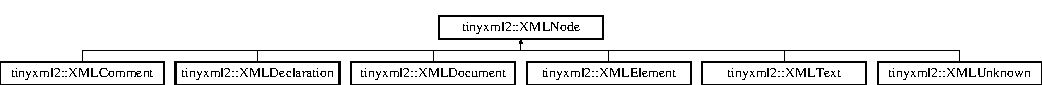
\includegraphics[height=1.145194cm]{classtinyxml2_1_1_x_m_l_node}
\end{center}
\end{figure}
\subsection*{Public Member Functions}
\begin{DoxyCompactItemize}
\item 
const \hyperlink{classtinyxml2_1_1_x_m_l_document}{X\-M\-L\-Document} $\ast$ \hyperlink{classtinyxml2_1_1_x_m_l_node_add244bca368083fa29698db8dcf147ca}{Get\-Document} () const 
\begin{DoxyCompactList}\small\item\em Get the \hyperlink{classtinyxml2_1_1_x_m_l_document}{X\-M\-L\-Document} that owns this \hyperlink{classtinyxml2_1_1_x_m_l_node}{X\-M\-L\-Node}. \end{DoxyCompactList}\item 
\hyperlink{classtinyxml2_1_1_x_m_l_document}{X\-M\-L\-Document} $\ast$ \hyperlink{classtinyxml2_1_1_x_m_l_node_af343d1ef0b45c0020e62d784d7e67a68}{Get\-Document} ()
\begin{DoxyCompactList}\small\item\em Get the \hyperlink{classtinyxml2_1_1_x_m_l_document}{X\-M\-L\-Document} that owns this \hyperlink{classtinyxml2_1_1_x_m_l_node}{X\-M\-L\-Node}. \end{DoxyCompactList}\item 
virtual \hyperlink{classtinyxml2_1_1_x_m_l_element}{X\-M\-L\-Element} $\ast$ \hyperlink{classtinyxml2_1_1_x_m_l_node_aab516e699567f75cc9ab2ef2eee501e8}{To\-Element} ()
\begin{DoxyCompactList}\small\item\em Safely cast to an Element, or null. \end{DoxyCompactList}\item 
virtual \hyperlink{classtinyxml2_1_1_x_m_l_text}{X\-M\-L\-Text} $\ast$ \hyperlink{classtinyxml2_1_1_x_m_l_node_a41c55dab9162d1eb62db2008430e376b}{To\-Text} ()
\begin{DoxyCompactList}\small\item\em Safely cast to Text, or null. \end{DoxyCompactList}\item 
virtual \hyperlink{classtinyxml2_1_1_x_m_l_comment}{X\-M\-L\-Comment} $\ast$ \hyperlink{classtinyxml2_1_1_x_m_l_node_aff47671055aa99840a1c1ebd661e63e3}{To\-Comment} ()
\begin{DoxyCompactList}\small\item\em Safely cast to a Comment, or null. \end{DoxyCompactList}\item 
virtual \hyperlink{classtinyxml2_1_1_x_m_l_document}{X\-M\-L\-Document} $\ast$ \hyperlink{classtinyxml2_1_1_x_m_l_node_a836e2966ed736fc3c94f70e12a2a3357}{To\-Document} ()
\begin{DoxyCompactList}\small\item\em Safely cast to a Document, or null. \end{DoxyCompactList}\item 
virtual \hyperlink{classtinyxml2_1_1_x_m_l_declaration}{X\-M\-L\-Declaration} $\ast$ \hyperlink{classtinyxml2_1_1_x_m_l_node_a174fd4c22c010b58138c1b84a0dfbd51}{To\-Declaration} ()
\begin{DoxyCompactList}\small\item\em Safely cast to a Declaration, or null. \end{DoxyCompactList}\item 
virtual \hyperlink{classtinyxml2_1_1_x_m_l_unknown}{X\-M\-L\-Unknown} $\ast$ \hyperlink{classtinyxml2_1_1_x_m_l_node_a8675a74aa0ada6eccab0c77ef3e5b9bd}{To\-Unknown} ()
\begin{DoxyCompactList}\small\item\em Safely cast to an Unknown, or null. \end{DoxyCompactList}\item 
virtual const \hyperlink{classtinyxml2_1_1_x_m_l_element}{X\-M\-L\-Element} $\ast$ \hyperlink{classtinyxml2_1_1_x_m_l_node_acbaec609797ddabb4f9dcf38ee91262e}{To\-Element} () const 
\item 
virtual const \hyperlink{classtinyxml2_1_1_x_m_l_text}{X\-M\-L\-Text} $\ast$ \hyperlink{classtinyxml2_1_1_x_m_l_node_a89009ffc1b9f5d692bf8d4c9f18c3bec}{To\-Text} () const 
\item 
virtual const \hyperlink{classtinyxml2_1_1_x_m_l_comment}{X\-M\-L\-Comment} $\ast$ \hyperlink{classtinyxml2_1_1_x_m_l_node_a157ce3a00ea5ee5a85b7103138e85e8a}{To\-Comment} () const 
\item 
virtual const \hyperlink{classtinyxml2_1_1_x_m_l_document}{X\-M\-L\-Document} $\ast$ \hyperlink{classtinyxml2_1_1_x_m_l_node_a3ff975733a17d6ced3539b45544c8bf6}{To\-Document} () const 
\item 
virtual const \hyperlink{classtinyxml2_1_1_x_m_l_declaration}{X\-M\-L\-Declaration} $\ast$ \hyperlink{classtinyxml2_1_1_x_m_l_node_aedae0bbb58d533a4b8a61042388b49e5}{To\-Declaration} () const 
\item 
virtual const \hyperlink{classtinyxml2_1_1_x_m_l_unknown}{X\-M\-L\-Unknown} $\ast$ \hyperlink{classtinyxml2_1_1_x_m_l_node_a71f5ae90296dbe67979f83fe97073efa}{To\-Unknown} () const 
\item 
const char $\ast$ \hyperlink{classtinyxml2_1_1_x_m_l_node_a7682be117e3b2b4ebfd517c1acaaadbf}{Value} () const 
\item 
void \hyperlink{classtinyxml2_1_1_x_m_l_node_a09dd68cf9eae137579f6e50f36487513}{Set\-Value} (const char $\ast$val, bool static\-Mem=false)
\item 
const \hyperlink{classtinyxml2_1_1_x_m_l_node}{X\-M\-L\-Node} $\ast$ \hyperlink{classtinyxml2_1_1_x_m_l_node_a4e39bdcf9bfafa55d04857ece6aaf64e}{Parent} () const 
\begin{DoxyCompactList}\small\item\em Get the parent of this node on the D\-O\-M. \end{DoxyCompactList}\item 
\hyperlink{classtinyxml2_1_1_x_m_l_node}{X\-M\-L\-Node} $\ast$ \hyperlink{classtinyxml2_1_1_x_m_l_node_a76029693a5a54fbb721a41d7a0ca8a97}{Parent} ()
\item 
bool \hyperlink{classtinyxml2_1_1_x_m_l_node_a96afe34a9ccd0ed4c0cff32beb42cc6c}{No\-Children} () const 
\begin{DoxyCompactList}\small\item\em Returns true if this node has no children. \end{DoxyCompactList}\item 
const \hyperlink{classtinyxml2_1_1_x_m_l_node}{X\-M\-L\-Node} $\ast$ \hyperlink{classtinyxml2_1_1_x_m_l_node_a60e923d13d7dc01f45ab90a2f948b02a}{First\-Child} () const 
\begin{DoxyCompactList}\small\item\em Get the first child node, or null if none exists. \end{DoxyCompactList}\item 
\hyperlink{classtinyxml2_1_1_x_m_l_node}{X\-M\-L\-Node} $\ast$ \hyperlink{classtinyxml2_1_1_x_m_l_node_a2d6c70c475146b48bc93a7fafdeff5e0}{First\-Child} ()
\item 
const \hyperlink{classtinyxml2_1_1_x_m_l_element}{X\-M\-L\-Element} $\ast$ \hyperlink{classtinyxml2_1_1_x_m_l_node_a20f48e99b03e9c17487944f229bee130}{First\-Child\-Element} (const char $\ast$value=0) const 
\item 
\hyperlink{classtinyxml2_1_1_x_m_l_element}{X\-M\-L\-Element} $\ast$ \hyperlink{classtinyxml2_1_1_x_m_l_node_a7614c3b4eea1ff11b2aa90b0f92f6dba}{First\-Child\-Element} (const char $\ast$value=0)
\item 
const \hyperlink{classtinyxml2_1_1_x_m_l_node}{X\-M\-L\-Node} $\ast$ \hyperlink{classtinyxml2_1_1_x_m_l_node_a6088246532b02895beb0e6fa561a7f3b}{Last\-Child} () const 
\begin{DoxyCompactList}\small\item\em Get the last child node, or null if none exists. \end{DoxyCompactList}\item 
\hyperlink{classtinyxml2_1_1_x_m_l_node}{X\-M\-L\-Node} $\ast$ \hyperlink{classtinyxml2_1_1_x_m_l_node_ad7552c8cb1dc0cb6f3bdc14a9d115dbf}{Last\-Child} ()
\item 
const \hyperlink{classtinyxml2_1_1_x_m_l_element}{X\-M\-L\-Element} $\ast$ \hyperlink{classtinyxml2_1_1_x_m_l_node_a1a46cc01ece2216acf1e6294d1aff79d}{Last\-Child\-Element} (const char $\ast$value=0) const 
\item 
\hyperlink{classtinyxml2_1_1_x_m_l_element}{X\-M\-L\-Element} $\ast$ \hyperlink{classtinyxml2_1_1_x_m_l_node_a125423acf3170b130634638c5afc0639}{Last\-Child\-Element} (const char $\ast$value=0)
\item 
const \hyperlink{classtinyxml2_1_1_x_m_l_node}{X\-M\-L\-Node} $\ast$ \hyperlink{classtinyxml2_1_1_x_m_l_node_a4cb1bf63e9de55129d21a7be60685fd4}{Previous\-Sibling} () const 
\begin{DoxyCompactList}\small\item\em Get the previous (left) sibling node of this node. \end{DoxyCompactList}\item 
\hyperlink{classtinyxml2_1_1_x_m_l_node}{X\-M\-L\-Node} $\ast$ \hyperlink{classtinyxml2_1_1_x_m_l_node_ae760e5e7e766df1d2cf3bb4a847876d6}{Previous\-Sibling} ()
\item 
const \hyperlink{classtinyxml2_1_1_x_m_l_element}{X\-M\-L\-Element} $\ast$ \hyperlink{classtinyxml2_1_1_x_m_l_node_a573b2559c41dce244d893d610fbe0bd9}{Previous\-Sibling\-Element} (const char $\ast$value=0) const 
\begin{DoxyCompactList}\small\item\em Get the previous (left) sibling element of this node, with an optionally supplied name. \end{DoxyCompactList}\item 
\hyperlink{classtinyxml2_1_1_x_m_l_element}{X\-M\-L\-Element} $\ast$ \hyperlink{classtinyxml2_1_1_x_m_l_node_ae9177fdc49cb89879f333581d5f734f1}{Previous\-Sibling\-Element} (const char $\ast$value=0)
\item 
const \hyperlink{classtinyxml2_1_1_x_m_l_node}{X\-M\-L\-Node} $\ast$ \hyperlink{classtinyxml2_1_1_x_m_l_node_abba1df37581d89dccc45acdc55750ba2}{Next\-Sibling} () const 
\begin{DoxyCompactList}\small\item\em Get the next (right) sibling node of this node. \end{DoxyCompactList}\item 
\hyperlink{classtinyxml2_1_1_x_m_l_node}{X\-M\-L\-Node} $\ast$ \hyperlink{classtinyxml2_1_1_x_m_l_node_aeb7d4dfd8fb924ef86e7cb72183acbac}{Next\-Sibling} ()
\item 
const \hyperlink{classtinyxml2_1_1_x_m_l_element}{X\-M\-L\-Element} $\ast$ \hyperlink{classtinyxml2_1_1_x_m_l_node_a490e166c3a1c6607960bfa9c112d3d30}{Next\-Sibling\-Element} (const char $\ast$value=0) const 
\begin{DoxyCompactList}\small\item\em Get the next (right) sibling element of this node, with an optionally supplied name. \end{DoxyCompactList}\item 
\hyperlink{classtinyxml2_1_1_x_m_l_element}{X\-M\-L\-Element} $\ast$ \hyperlink{classtinyxml2_1_1_x_m_l_node_acf735bf653016792522305d8ad4b3029}{Next\-Sibling\-Element} (const char $\ast$value=0)
\item 
\hyperlink{classtinyxml2_1_1_x_m_l_node}{X\-M\-L\-Node} $\ast$ \hyperlink{classtinyxml2_1_1_x_m_l_node_ae3b422e98914d6002ca99bb1d2837103}{Insert\-End\-Child} (\hyperlink{classtinyxml2_1_1_x_m_l_node}{X\-M\-L\-Node} $\ast$add\-This)
\item 
\hyperlink{classtinyxml2_1_1_x_m_l_node}{X\-M\-L\-Node} $\ast$ \hyperlink{classtinyxml2_1_1_x_m_l_node_a663e3a5a378169fd477378f4d17a7649}{Link\-End\-Child} (\hyperlink{classtinyxml2_1_1_x_m_l_node}{X\-M\-L\-Node} $\ast$add\-This)
\item 
\hyperlink{classtinyxml2_1_1_x_m_l_node}{X\-M\-L\-Node} $\ast$ \hyperlink{classtinyxml2_1_1_x_m_l_node_ac609a8f3ea949027f439280c640bbaf2}{Insert\-First\-Child} (\hyperlink{classtinyxml2_1_1_x_m_l_node}{X\-M\-L\-Node} $\ast$add\-This)
\item 
\hyperlink{classtinyxml2_1_1_x_m_l_node}{X\-M\-L\-Node} $\ast$ \hyperlink{classtinyxml2_1_1_x_m_l_node_a9275138a1b8dd5d8e2c26789bdc23ac8}{Insert\-After\-Child} (\hyperlink{classtinyxml2_1_1_x_m_l_node}{X\-M\-L\-Node} $\ast$after\-This, \hyperlink{classtinyxml2_1_1_x_m_l_node}{X\-M\-L\-Node} $\ast$add\-This)
\item 
void \hyperlink{classtinyxml2_1_1_x_m_l_node_a0360085cc54df5bff85d5c5da13afdce}{Delete\-Children} ()
\item 
void \hyperlink{classtinyxml2_1_1_x_m_l_node_a363b6edbd6ebd55f8387d2b89f2b0921}{Delete\-Child} (\hyperlink{classtinyxml2_1_1_x_m_l_node}{X\-M\-L\-Node} $\ast$node)
\item 
virtual \hyperlink{classtinyxml2_1_1_x_m_l_node}{X\-M\-L\-Node} $\ast$ \hyperlink{classtinyxml2_1_1_x_m_l_node_a8402cbd3129d20e9e6024bbcc0531283}{Shallow\-Clone} (\hyperlink{classtinyxml2_1_1_x_m_l_document}{X\-M\-L\-Document} $\ast$document) const =0
\item 
virtual bool \hyperlink{classtinyxml2_1_1_x_m_l_node_a7ce18b751c3ea09eac292dca264f9226}{Shallow\-Equal} (const \hyperlink{classtinyxml2_1_1_x_m_l_node}{X\-M\-L\-Node} $\ast$compare) const =0
\item 
virtual bool \hyperlink{classtinyxml2_1_1_x_m_l_node_a81e66df0a44c67a7af17f3b77a152785}{Accept} (\hyperlink{classtinyxml2_1_1_x_m_l_visitor}{X\-M\-L\-Visitor} $\ast$visitor) const =0
\item 
virtual char $\ast$ \hyperlink{classtinyxml2_1_1_x_m_l_node_a7610d0f603e8b603d2078521811a23c1}{Parse\-Deep} (char $\ast$, \hyperlink{classtinyxml2_1_1_str_pair}{Str\-Pair} $\ast$)
\end{DoxyCompactItemize}
\subsection*{Protected Member Functions}
\begin{DoxyCompactItemize}
\item 
\hyperlink{classtinyxml2_1_1_x_m_l_node_a29868df6ca383d574f584dfdd15105b6}{X\-M\-L\-Node} (\hyperlink{classtinyxml2_1_1_x_m_l_document}{X\-M\-L\-Document} $\ast$)
\item 
virtual \hyperlink{classtinyxml2_1_1_x_m_l_node_a8f41e898cdd4da4cdbb7f05b0c7d9f69}{$\sim$\-X\-M\-L\-Node} ()
\item 
\hyperlink{classtinyxml2_1_1_x_m_l_node_a78be01384518a969da905548f318d75b}{X\-M\-L\-Node} (const \hyperlink{classtinyxml2_1_1_x_m_l_node}{X\-M\-L\-Node} \&)
\item 
\hyperlink{classtinyxml2_1_1_x_m_l_node}{X\-M\-L\-Node} \& \hyperlink{classtinyxml2_1_1_x_m_l_node_ade79231d908e1f21862819e00e56ab6e}{operator=} (const \hyperlink{classtinyxml2_1_1_x_m_l_node}{X\-M\-L\-Node} \&)
\end{DoxyCompactItemize}
\subsection*{Protected Attributes}
\begin{DoxyCompactItemize}
\item 
\hyperlink{classtinyxml2_1_1_x_m_l_document}{X\-M\-L\-Document} $\ast$ \hyperlink{classtinyxml2_1_1_x_m_l_node_a8d2d2be0bb6797625551eb0e91f0ff62}{\-\_\-document}
\item 
\hyperlink{classtinyxml2_1_1_x_m_l_node}{X\-M\-L\-Node} $\ast$ \hyperlink{classtinyxml2_1_1_x_m_l_node_a176dd1c4965c21c366de192164aa2c13}{\-\_\-parent}
\item 
\hyperlink{classtinyxml2_1_1_str_pair}{Str\-Pair} \hyperlink{classtinyxml2_1_1_x_m_l_node_a3ea9884098b8379de2bb5ab3fc85c0fc}{\-\_\-value}
\item 
\hyperlink{classtinyxml2_1_1_x_m_l_node}{X\-M\-L\-Node} $\ast$ \hyperlink{classtinyxml2_1_1_x_m_l_node_aa20c91e4213dc930c5bdf420322ca342}{\-\_\-first\-Child}
\item 
\hyperlink{classtinyxml2_1_1_x_m_l_node}{X\-M\-L\-Node} $\ast$ \hyperlink{classtinyxml2_1_1_x_m_l_node_a099b6560ae44ab9edb8453aaf1a3747b}{\-\_\-last\-Child}
\item 
\hyperlink{classtinyxml2_1_1_x_m_l_node}{X\-M\-L\-Node} $\ast$ \hyperlink{classtinyxml2_1_1_x_m_l_node_a9739eb0fb9a1188266052055e7a6bf6b}{\-\_\-prev}
\item 
\hyperlink{classtinyxml2_1_1_x_m_l_node}{X\-M\-L\-Node} $\ast$ \hyperlink{classtinyxml2_1_1_x_m_l_node_a27e985496b37dd00eb5b9cf59b9e3fb1}{\-\_\-next}
\end{DoxyCompactItemize}
\subsection*{Friends}
\begin{DoxyCompactItemize}
\item 
class \hyperlink{classtinyxml2_1_1_x_m_l_node_a4eee3bda60c60a30e4e8cd4ea91c4c6e}{X\-M\-L\-Document}
\item 
class \hyperlink{classtinyxml2_1_1_x_m_l_node_ac2fba9b6e452829dd892f7392c24e0eb}{X\-M\-L\-Element}
\end{DoxyCompactItemize}


\subsection{Detailed Description}
\hyperlink{classtinyxml2_1_1_x_m_l_node}{X\-M\-L\-Node} is a base class for every object that is in the X\-M\-L Document Object Model (D\-O\-M), except X\-M\-L\-Attributes. Nodes have siblings, a parent, and children which can be navigated. A node is always in a \hyperlink{classtinyxml2_1_1_x_m_l_document}{X\-M\-L\-Document}. The type of a \hyperlink{classtinyxml2_1_1_x_m_l_node}{X\-M\-L\-Node} can be queried, and it can be cast to its more defined type.

A \hyperlink{classtinyxml2_1_1_x_m_l_document}{X\-M\-L\-Document} allocates memory for all its Nodes. When the \hyperlink{classtinyxml2_1_1_x_m_l_document}{X\-M\-L\-Document} gets deleted, all its Nodes will also be deleted.

\begin{DoxyVerb}A Document can contain: Element (container or leaf)
                        Comment (leaf)
                        Unknown (leaf)
                        Declaration( leaf )

An Element can contain: Element (container or leaf)
                        Text    (leaf)
                        Attributes (not on tree)
                        Comment (leaf)
                        Unknown (leaf)\end{DoxyVerb}
 

Definition at line 573 of file tinyxml2.\-hpp.



\subsection{Constructor \& Destructor Documentation}
\hypertarget{classtinyxml2_1_1_x_m_l_node_a29868df6ca383d574f584dfdd15105b6}{\index{tinyxml2\-::\-X\-M\-L\-Node@{tinyxml2\-::\-X\-M\-L\-Node}!X\-M\-L\-Node@{X\-M\-L\-Node}}
\index{X\-M\-L\-Node@{X\-M\-L\-Node}!tinyxml2::XMLNode@{tinyxml2\-::\-X\-M\-L\-Node}}
\subsubsection[{X\-M\-L\-Node}]{\setlength{\rightskip}{0pt plus 5cm}tinyxml2\-::\-X\-M\-L\-Node\-::\-X\-M\-L\-Node (
\begin{DoxyParamCaption}
\item[{{\bf X\-M\-L\-Document} $\ast$}]{doc}
\end{DoxyParamCaption}
)\hspace{0.3cm}{\ttfamily [protected]}}}\label{classtinyxml2_1_1_x_m_l_node_a29868df6ca383d574f584dfdd15105b6}


Definition at line 580 of file tinyxml2.\-cpp.

\hypertarget{classtinyxml2_1_1_x_m_l_node_a8f41e898cdd4da4cdbb7f05b0c7d9f69}{\index{tinyxml2\-::\-X\-M\-L\-Node@{tinyxml2\-::\-X\-M\-L\-Node}!$\sim$\-X\-M\-L\-Node@{$\sim$\-X\-M\-L\-Node}}
\index{$\sim$\-X\-M\-L\-Node@{$\sim$\-X\-M\-L\-Node}!tinyxml2::XMLNode@{tinyxml2\-::\-X\-M\-L\-Node}}
\subsubsection[{$\sim$\-X\-M\-L\-Node}]{\setlength{\rightskip}{0pt plus 5cm}tinyxml2\-::\-X\-M\-L\-Node\-::$\sim$\-X\-M\-L\-Node (
\begin{DoxyParamCaption}
{}
\end{DoxyParamCaption}
)\hspace{0.3cm}{\ttfamily [protected]}, {\ttfamily [virtual]}}}\label{classtinyxml2_1_1_x_m_l_node_a8f41e898cdd4da4cdbb7f05b0c7d9f69}


Definition at line 590 of file tinyxml2.\-cpp.

\hypertarget{classtinyxml2_1_1_x_m_l_node_a78be01384518a969da905548f318d75b}{\index{tinyxml2\-::\-X\-M\-L\-Node@{tinyxml2\-::\-X\-M\-L\-Node}!X\-M\-L\-Node@{X\-M\-L\-Node}}
\index{X\-M\-L\-Node@{X\-M\-L\-Node}!tinyxml2::XMLNode@{tinyxml2\-::\-X\-M\-L\-Node}}
\subsubsection[{X\-M\-L\-Node}]{\setlength{\rightskip}{0pt plus 5cm}tinyxml2\-::\-X\-M\-L\-Node\-::\-X\-M\-L\-Node (
\begin{DoxyParamCaption}
\item[{const {\bf X\-M\-L\-Node} \&}]{}
\end{DoxyParamCaption}
)\hspace{0.3cm}{\ttfamily [protected]}}}\label{classtinyxml2_1_1_x_m_l_node_a78be01384518a969da905548f318d75b}


\subsection{Member Function Documentation}
\hypertarget{classtinyxml2_1_1_x_m_l_node_a81e66df0a44c67a7af17f3b77a152785}{\index{tinyxml2\-::\-X\-M\-L\-Node@{tinyxml2\-::\-X\-M\-L\-Node}!Accept@{Accept}}
\index{Accept@{Accept}!tinyxml2::XMLNode@{tinyxml2\-::\-X\-M\-L\-Node}}
\subsubsection[{Accept}]{\setlength{\rightskip}{0pt plus 5cm}virtual bool tinyxml2\-::\-X\-M\-L\-Node\-::\-Accept (
\begin{DoxyParamCaption}
\item[{{\bf X\-M\-L\-Visitor} $\ast$}]{visitor}
\end{DoxyParamCaption}
) const\hspace{0.3cm}{\ttfamily [pure virtual]}}}\label{classtinyxml2_1_1_x_m_l_node_a81e66df0a44c67a7af17f3b77a152785}
Accept a hierarchical visit of the nodes in the Tiny\-X\-M\-L-\/2 D\-O\-M. Every node in the X\-M\-L tree will be conditionally visited and the host will be called back via the \hyperlink{classtinyxml2_1_1_x_m_l_visitor}{X\-M\-L\-Visitor} interface.

This is essentially a S\-A\-X interface for Tiny\-X\-M\-L-\/2. (Note however it doesn't re-\/parse the X\-M\-L for the callbacks, so the performance of Tiny\-X\-M\-L-\/2 is unchanged by using this interface versus any other.)

The interface has been based on ideas from\-:
\begin{DoxyItemize}
\item \href{http://www.saxproject.org/}{\tt http\-://www.\-saxproject.\-org/}
\item \href{http://c2.com/cgi/wiki?HierarchicalVisitorPattern}{\tt http\-://c2.\-com/cgi/wiki?\-Hierarchical\-Visitor\-Pattern}
\end{DoxyItemize}

Which are both good references for \char`\"{}visiting\char`\"{}.

An example of using \hyperlink{classtinyxml2_1_1_x_m_l_node_a81e66df0a44c67a7af17f3b77a152785}{Accept()}\-: \begin{DoxyVerb}XMLPrinter printer;
tinyxmlDoc.Accept( &printer );
const char* xmlcstr = printer.CStr();
\end{DoxyVerb}
 

Implemented in \hyperlink{classtinyxml2_1_1_x_m_l_document_aa08503d24898bf9992ae5e5fb8b0cf87}{tinyxml2\-::\-X\-M\-L\-Document}, \hyperlink{classtinyxml2_1_1_x_m_l_element_a36d65438991a1e85096caf39ad13a099}{tinyxml2\-::\-X\-M\-L\-Element}, \hyperlink{classtinyxml2_1_1_x_m_l_unknown_a0d341ab804a1438a474810bb5bd29dd5}{tinyxml2\-::\-X\-M\-L\-Unknown}, \hyperlink{classtinyxml2_1_1_x_m_l_declaration_a953a7359cc312d15218eb5843a4ca108}{tinyxml2\-::\-X\-M\-L\-Declaration}, \hyperlink{classtinyxml2_1_1_x_m_l_comment_aa382b1be6a8b0650c16a2d88bb499335}{tinyxml2\-::\-X\-M\-L\-Comment}, and \hyperlink{classtinyxml2_1_1_x_m_l_text_ae659d4fc7351a7df11c111cbe1ade46f}{tinyxml2\-::\-X\-M\-L\-Text}.

\hypertarget{classtinyxml2_1_1_x_m_l_node_a363b6edbd6ebd55f8387d2b89f2b0921}{\index{tinyxml2\-::\-X\-M\-L\-Node@{tinyxml2\-::\-X\-M\-L\-Node}!Delete\-Child@{Delete\-Child}}
\index{Delete\-Child@{Delete\-Child}!tinyxml2::XMLNode@{tinyxml2\-::\-X\-M\-L\-Node}}
\subsubsection[{Delete\-Child}]{\setlength{\rightskip}{0pt plus 5cm}void tinyxml2\-::\-X\-M\-L\-Node\-::\-Delete\-Child (
\begin{DoxyParamCaption}
\item[{{\bf X\-M\-L\-Node} $\ast$}]{node}
\end{DoxyParamCaption}
)}}\label{classtinyxml2_1_1_x_m_l_node_a363b6edbd6ebd55f8387d2b89f2b0921}
Delete a child of this node. 

Definition at line 642 of file tinyxml2.\-cpp.

\hypertarget{classtinyxml2_1_1_x_m_l_node_a0360085cc54df5bff85d5c5da13afdce}{\index{tinyxml2\-::\-X\-M\-L\-Node@{tinyxml2\-::\-X\-M\-L\-Node}!Delete\-Children@{Delete\-Children}}
\index{Delete\-Children@{Delete\-Children}!tinyxml2::XMLNode@{tinyxml2\-::\-X\-M\-L\-Node}}
\subsubsection[{Delete\-Children}]{\setlength{\rightskip}{0pt plus 5cm}void tinyxml2\-::\-X\-M\-L\-Node\-::\-Delete\-Children (
\begin{DoxyParamCaption}
{}
\end{DoxyParamCaption}
)}}\label{classtinyxml2_1_1_x_m_l_node_a0360085cc54df5bff85d5c5da13afdce}
Delete all the children of this node. 

Definition at line 610 of file tinyxml2.\-cpp.

\hypertarget{classtinyxml2_1_1_x_m_l_node_a60e923d13d7dc01f45ab90a2f948b02a}{\index{tinyxml2\-::\-X\-M\-L\-Node@{tinyxml2\-::\-X\-M\-L\-Node}!First\-Child@{First\-Child}}
\index{First\-Child@{First\-Child}!tinyxml2::XMLNode@{tinyxml2\-::\-X\-M\-L\-Node}}
\subsubsection[{First\-Child}]{\setlength{\rightskip}{0pt plus 5cm}const {\bf X\-M\-L\-Node}$\ast$ tinyxml2\-::\-X\-M\-L\-Node\-::\-First\-Child (
\begin{DoxyParamCaption}
{}
\end{DoxyParamCaption}
) const\hspace{0.3cm}{\ttfamily [inline]}}}\label{classtinyxml2_1_1_x_m_l_node_a60e923d13d7dc01f45ab90a2f948b02a}


Get the first child node, or null if none exists. 



Definition at line 665 of file tinyxml2.\-hpp.

\hypertarget{classtinyxml2_1_1_x_m_l_node_a2d6c70c475146b48bc93a7fafdeff5e0}{\index{tinyxml2\-::\-X\-M\-L\-Node@{tinyxml2\-::\-X\-M\-L\-Node}!First\-Child@{First\-Child}}
\index{First\-Child@{First\-Child}!tinyxml2::XMLNode@{tinyxml2\-::\-X\-M\-L\-Node}}
\subsubsection[{First\-Child}]{\setlength{\rightskip}{0pt plus 5cm}{\bf X\-M\-L\-Node}$\ast$ tinyxml2\-::\-X\-M\-L\-Node\-::\-First\-Child (
\begin{DoxyParamCaption}
{}
\end{DoxyParamCaption}
)\hspace{0.3cm}{\ttfamily [inline]}}}\label{classtinyxml2_1_1_x_m_l_node_a2d6c70c475146b48bc93a7fafdeff5e0}


Definition at line 669 of file tinyxml2.\-hpp.

\hypertarget{classtinyxml2_1_1_x_m_l_node_a20f48e99b03e9c17487944f229bee130}{\index{tinyxml2\-::\-X\-M\-L\-Node@{tinyxml2\-::\-X\-M\-L\-Node}!First\-Child\-Element@{First\-Child\-Element}}
\index{First\-Child\-Element@{First\-Child\-Element}!tinyxml2::XMLNode@{tinyxml2\-::\-X\-M\-L\-Node}}
\subsubsection[{First\-Child\-Element}]{\setlength{\rightskip}{0pt plus 5cm}const {\bf X\-M\-L\-Element} $\ast$ tinyxml2\-::\-X\-M\-L\-Node\-::\-First\-Child\-Element (
\begin{DoxyParamCaption}
\item[{const char $\ast$}]{value = {\ttfamily 0}}
\end{DoxyParamCaption}
) const}}\label{classtinyxml2_1_1_x_m_l_node_a20f48e99b03e9c17487944f229bee130}
Get the first child element, or optionally the first child element with the specified name. 

Definition at line 721 of file tinyxml2.\-cpp.

\hypertarget{classtinyxml2_1_1_x_m_l_node_a7614c3b4eea1ff11b2aa90b0f92f6dba}{\index{tinyxml2\-::\-X\-M\-L\-Node@{tinyxml2\-::\-X\-M\-L\-Node}!First\-Child\-Element@{First\-Child\-Element}}
\index{First\-Child\-Element@{First\-Child\-Element}!tinyxml2::XMLNode@{tinyxml2\-::\-X\-M\-L\-Node}}
\subsubsection[{First\-Child\-Element}]{\setlength{\rightskip}{0pt plus 5cm}{\bf X\-M\-L\-Element}$\ast$ tinyxml2\-::\-X\-M\-L\-Node\-::\-First\-Child\-Element (
\begin{DoxyParamCaption}
\item[{const char $\ast$}]{value = {\ttfamily 0}}
\end{DoxyParamCaption}
)\hspace{0.3cm}{\ttfamily [inline]}}}\label{classtinyxml2_1_1_x_m_l_node_a7614c3b4eea1ff11b2aa90b0f92f6dba}


Definition at line 678 of file tinyxml2.\-hpp.

\hypertarget{classtinyxml2_1_1_x_m_l_node_add244bca368083fa29698db8dcf147ca}{\index{tinyxml2\-::\-X\-M\-L\-Node@{tinyxml2\-::\-X\-M\-L\-Node}!Get\-Document@{Get\-Document}}
\index{Get\-Document@{Get\-Document}!tinyxml2::XMLNode@{tinyxml2\-::\-X\-M\-L\-Node}}
\subsubsection[{Get\-Document}]{\setlength{\rightskip}{0pt plus 5cm}const {\bf X\-M\-L\-Document}$\ast$ tinyxml2\-::\-X\-M\-L\-Node\-::\-Get\-Document (
\begin{DoxyParamCaption}
{}
\end{DoxyParamCaption}
) const\hspace{0.3cm}{\ttfamily [inline]}}}\label{classtinyxml2_1_1_x_m_l_node_add244bca368083fa29698db8dcf147ca}


Get the \hyperlink{classtinyxml2_1_1_x_m_l_document}{X\-M\-L\-Document} that owns this \hyperlink{classtinyxml2_1_1_x_m_l_node}{X\-M\-L\-Node}. 



Definition at line 580 of file tinyxml2.\-hpp.

\hypertarget{classtinyxml2_1_1_x_m_l_node_af343d1ef0b45c0020e62d784d7e67a68}{\index{tinyxml2\-::\-X\-M\-L\-Node@{tinyxml2\-::\-X\-M\-L\-Node}!Get\-Document@{Get\-Document}}
\index{Get\-Document@{Get\-Document}!tinyxml2::XMLNode@{tinyxml2\-::\-X\-M\-L\-Node}}
\subsubsection[{Get\-Document}]{\setlength{\rightskip}{0pt plus 5cm}{\bf X\-M\-L\-Document}$\ast$ tinyxml2\-::\-X\-M\-L\-Node\-::\-Get\-Document (
\begin{DoxyParamCaption}
{}
\end{DoxyParamCaption}
)\hspace{0.3cm}{\ttfamily [inline]}}}\label{classtinyxml2_1_1_x_m_l_node_af343d1ef0b45c0020e62d784d7e67a68}


Get the \hyperlink{classtinyxml2_1_1_x_m_l_document}{X\-M\-L\-Document} that owns this \hyperlink{classtinyxml2_1_1_x_m_l_node}{X\-M\-L\-Node}. 



Definition at line 584 of file tinyxml2.\-hpp.

\hypertarget{classtinyxml2_1_1_x_m_l_node_a9275138a1b8dd5d8e2c26789bdc23ac8}{\index{tinyxml2\-::\-X\-M\-L\-Node@{tinyxml2\-::\-X\-M\-L\-Node}!Insert\-After\-Child@{Insert\-After\-Child}}
\index{Insert\-After\-Child@{Insert\-After\-Child}!tinyxml2::XMLNode@{tinyxml2\-::\-X\-M\-L\-Node}}
\subsubsection[{Insert\-After\-Child}]{\setlength{\rightskip}{0pt plus 5cm}{\bf X\-M\-L\-Node} $\ast$ tinyxml2\-::\-X\-M\-L\-Node\-::\-Insert\-After\-Child (
\begin{DoxyParamCaption}
\item[{{\bf X\-M\-L\-Node} $\ast$}]{after\-This, }
\item[{{\bf X\-M\-L\-Node} $\ast$}]{add\-This}
\end{DoxyParamCaption}
)}}\label{classtinyxml2_1_1_x_m_l_node_a9275138a1b8dd5d8e2c26789bdc23ac8}
Add a node after the specified child node. 

Definition at line 698 of file tinyxml2.\-cpp.

\hypertarget{classtinyxml2_1_1_x_m_l_node_ae3b422e98914d6002ca99bb1d2837103}{\index{tinyxml2\-::\-X\-M\-L\-Node@{tinyxml2\-::\-X\-M\-L\-Node}!Insert\-End\-Child@{Insert\-End\-Child}}
\index{Insert\-End\-Child@{Insert\-End\-Child}!tinyxml2::XMLNode@{tinyxml2\-::\-X\-M\-L\-Node}}
\subsubsection[{Insert\-End\-Child}]{\setlength{\rightskip}{0pt plus 5cm}{\bf X\-M\-L\-Node} $\ast$ tinyxml2\-::\-X\-M\-L\-Node\-::\-Insert\-End\-Child (
\begin{DoxyParamCaption}
\item[{{\bf X\-M\-L\-Node} $\ast$}]{add\-This}
\end{DoxyParamCaption}
)}}\label{classtinyxml2_1_1_x_m_l_node_ae3b422e98914d6002ca99bb1d2837103}
Add a child node as the last (right) child. 

Definition at line 649 of file tinyxml2.\-cpp.

\hypertarget{classtinyxml2_1_1_x_m_l_node_ac609a8f3ea949027f439280c640bbaf2}{\index{tinyxml2\-::\-X\-M\-L\-Node@{tinyxml2\-::\-X\-M\-L\-Node}!Insert\-First\-Child@{Insert\-First\-Child}}
\index{Insert\-First\-Child@{Insert\-First\-Child}!tinyxml2::XMLNode@{tinyxml2\-::\-X\-M\-L\-Node}}
\subsubsection[{Insert\-First\-Child}]{\setlength{\rightskip}{0pt plus 5cm}{\bf X\-M\-L\-Node} $\ast$ tinyxml2\-::\-X\-M\-L\-Node\-::\-Insert\-First\-Child (
\begin{DoxyParamCaption}
\item[{{\bf X\-M\-L\-Node} $\ast$}]{add\-This}
\end{DoxyParamCaption}
)}}\label{classtinyxml2_1_1_x_m_l_node_ac609a8f3ea949027f439280c640bbaf2}
Add a child node as the first (left) child. 

Definition at line 673 of file tinyxml2.\-cpp.

\hypertarget{classtinyxml2_1_1_x_m_l_node_a6088246532b02895beb0e6fa561a7f3b}{\index{tinyxml2\-::\-X\-M\-L\-Node@{tinyxml2\-::\-X\-M\-L\-Node}!Last\-Child@{Last\-Child}}
\index{Last\-Child@{Last\-Child}!tinyxml2::XMLNode@{tinyxml2\-::\-X\-M\-L\-Node}}
\subsubsection[{Last\-Child}]{\setlength{\rightskip}{0pt plus 5cm}const {\bf X\-M\-L\-Node}$\ast$ tinyxml2\-::\-X\-M\-L\-Node\-::\-Last\-Child (
\begin{DoxyParamCaption}
{}
\end{DoxyParamCaption}
) const\hspace{0.3cm}{\ttfamily [inline]}}}\label{classtinyxml2_1_1_x_m_l_node_a6088246532b02895beb0e6fa561a7f3b}


Get the last child node, or null if none exists. 



Definition at line 683 of file tinyxml2.\-hpp.

\hypertarget{classtinyxml2_1_1_x_m_l_node_ad7552c8cb1dc0cb6f3bdc14a9d115dbf}{\index{tinyxml2\-::\-X\-M\-L\-Node@{tinyxml2\-::\-X\-M\-L\-Node}!Last\-Child@{Last\-Child}}
\index{Last\-Child@{Last\-Child}!tinyxml2::XMLNode@{tinyxml2\-::\-X\-M\-L\-Node}}
\subsubsection[{Last\-Child}]{\setlength{\rightskip}{0pt plus 5cm}{\bf X\-M\-L\-Node}$\ast$ tinyxml2\-::\-X\-M\-L\-Node\-::\-Last\-Child (
\begin{DoxyParamCaption}
{}
\end{DoxyParamCaption}
)\hspace{0.3cm}{\ttfamily [inline]}}}\label{classtinyxml2_1_1_x_m_l_node_ad7552c8cb1dc0cb6f3bdc14a9d115dbf}


Definition at line 687 of file tinyxml2.\-hpp.

\hypertarget{classtinyxml2_1_1_x_m_l_node_a1a46cc01ece2216acf1e6294d1aff79d}{\index{tinyxml2\-::\-X\-M\-L\-Node@{tinyxml2\-::\-X\-M\-L\-Node}!Last\-Child\-Element@{Last\-Child\-Element}}
\index{Last\-Child\-Element@{Last\-Child\-Element}!tinyxml2::XMLNode@{tinyxml2\-::\-X\-M\-L\-Node}}
\subsubsection[{Last\-Child\-Element}]{\setlength{\rightskip}{0pt plus 5cm}const {\bf X\-M\-L\-Element} $\ast$ tinyxml2\-::\-X\-M\-L\-Node\-::\-Last\-Child\-Element (
\begin{DoxyParamCaption}
\item[{const char $\ast$}]{value = {\ttfamily 0}}
\end{DoxyParamCaption}
) const}}\label{classtinyxml2_1_1_x_m_l_node_a1a46cc01ece2216acf1e6294d1aff79d}
Get the last child element or optionally the last child element with the specified name. 

Definition at line 735 of file tinyxml2.\-cpp.

\hypertarget{classtinyxml2_1_1_x_m_l_node_a125423acf3170b130634638c5afc0639}{\index{tinyxml2\-::\-X\-M\-L\-Node@{tinyxml2\-::\-X\-M\-L\-Node}!Last\-Child\-Element@{Last\-Child\-Element}}
\index{Last\-Child\-Element@{Last\-Child\-Element}!tinyxml2::XMLNode@{tinyxml2\-::\-X\-M\-L\-Node}}
\subsubsection[{Last\-Child\-Element}]{\setlength{\rightskip}{0pt plus 5cm}{\bf X\-M\-L\-Element}$\ast$ tinyxml2\-::\-X\-M\-L\-Node\-::\-Last\-Child\-Element (
\begin{DoxyParamCaption}
\item[{const char $\ast$}]{value = {\ttfamily 0}}
\end{DoxyParamCaption}
)\hspace{0.3cm}{\ttfamily [inline]}}}\label{classtinyxml2_1_1_x_m_l_node_a125423acf3170b130634638c5afc0639}


Definition at line 696 of file tinyxml2.\-hpp.

\hypertarget{classtinyxml2_1_1_x_m_l_node_a663e3a5a378169fd477378f4d17a7649}{\index{tinyxml2\-::\-X\-M\-L\-Node@{tinyxml2\-::\-X\-M\-L\-Node}!Link\-End\-Child@{Link\-End\-Child}}
\index{Link\-End\-Child@{Link\-End\-Child}!tinyxml2::XMLNode@{tinyxml2\-::\-X\-M\-L\-Node}}
\subsubsection[{Link\-End\-Child}]{\setlength{\rightskip}{0pt plus 5cm}{\bf X\-M\-L\-Node}$\ast$ tinyxml2\-::\-X\-M\-L\-Node\-::\-Link\-End\-Child (
\begin{DoxyParamCaption}
\item[{{\bf X\-M\-L\-Node} $\ast$}]{add\-This}
\end{DoxyParamCaption}
)\hspace{0.3cm}{\ttfamily [inline]}}}\label{classtinyxml2_1_1_x_m_l_node_a663e3a5a378169fd477378f4d17a7649}


Definition at line 737 of file tinyxml2.\-hpp.

\hypertarget{classtinyxml2_1_1_x_m_l_node_abba1df37581d89dccc45acdc55750ba2}{\index{tinyxml2\-::\-X\-M\-L\-Node@{tinyxml2\-::\-X\-M\-L\-Node}!Next\-Sibling@{Next\-Sibling}}
\index{Next\-Sibling@{Next\-Sibling}!tinyxml2::XMLNode@{tinyxml2\-::\-X\-M\-L\-Node}}
\subsubsection[{Next\-Sibling}]{\setlength{\rightskip}{0pt plus 5cm}const {\bf X\-M\-L\-Node}$\ast$ tinyxml2\-::\-X\-M\-L\-Node\-::\-Next\-Sibling (
\begin{DoxyParamCaption}
{}
\end{DoxyParamCaption}
) const\hspace{0.3cm}{\ttfamily [inline]}}}\label{classtinyxml2_1_1_x_m_l_node_abba1df37581d89dccc45acdc55750ba2}


Get the next (right) sibling node of this node. 



Definition at line 717 of file tinyxml2.\-hpp.

\hypertarget{classtinyxml2_1_1_x_m_l_node_aeb7d4dfd8fb924ef86e7cb72183acbac}{\index{tinyxml2\-::\-X\-M\-L\-Node@{tinyxml2\-::\-X\-M\-L\-Node}!Next\-Sibling@{Next\-Sibling}}
\index{Next\-Sibling@{Next\-Sibling}!tinyxml2::XMLNode@{tinyxml2\-::\-X\-M\-L\-Node}}
\subsubsection[{Next\-Sibling}]{\setlength{\rightskip}{0pt plus 5cm}{\bf X\-M\-L\-Node}$\ast$ tinyxml2\-::\-X\-M\-L\-Node\-::\-Next\-Sibling (
\begin{DoxyParamCaption}
{}
\end{DoxyParamCaption}
)\hspace{0.3cm}{\ttfamily [inline]}}}\label{classtinyxml2_1_1_x_m_l_node_aeb7d4dfd8fb924ef86e7cb72183acbac}


Definition at line 721 of file tinyxml2.\-hpp.

\hypertarget{classtinyxml2_1_1_x_m_l_node_a490e166c3a1c6607960bfa9c112d3d30}{\index{tinyxml2\-::\-X\-M\-L\-Node@{tinyxml2\-::\-X\-M\-L\-Node}!Next\-Sibling\-Element@{Next\-Sibling\-Element}}
\index{Next\-Sibling\-Element@{Next\-Sibling\-Element}!tinyxml2::XMLNode@{tinyxml2\-::\-X\-M\-L\-Node}}
\subsubsection[{Next\-Sibling\-Element}]{\setlength{\rightskip}{0pt plus 5cm}const {\bf X\-M\-L\-Element} $\ast$ tinyxml2\-::\-X\-M\-L\-Node\-::\-Next\-Sibling\-Element (
\begin{DoxyParamCaption}
\item[{const char $\ast$}]{value = {\ttfamily 0}}
\end{DoxyParamCaption}
) const}}\label{classtinyxml2_1_1_x_m_l_node_a490e166c3a1c6607960bfa9c112d3d30}


Get the next (right) sibling element of this node, with an optionally supplied name. 



Definition at line 749 of file tinyxml2.\-cpp.

\hypertarget{classtinyxml2_1_1_x_m_l_node_acf735bf653016792522305d8ad4b3029}{\index{tinyxml2\-::\-X\-M\-L\-Node@{tinyxml2\-::\-X\-M\-L\-Node}!Next\-Sibling\-Element@{Next\-Sibling\-Element}}
\index{Next\-Sibling\-Element@{Next\-Sibling\-Element}!tinyxml2::XMLNode@{tinyxml2\-::\-X\-M\-L\-Node}}
\subsubsection[{Next\-Sibling\-Element}]{\setlength{\rightskip}{0pt plus 5cm}{\bf X\-M\-L\-Element}$\ast$ tinyxml2\-::\-X\-M\-L\-Node\-::\-Next\-Sibling\-Element (
\begin{DoxyParamCaption}
\item[{const char $\ast$}]{value = {\ttfamily 0}}
\end{DoxyParamCaption}
)\hspace{0.3cm}{\ttfamily [inline]}}}\label{classtinyxml2_1_1_x_m_l_node_acf735bf653016792522305d8ad4b3029}


Definition at line 728 of file tinyxml2.\-hpp.

\hypertarget{classtinyxml2_1_1_x_m_l_node_a96afe34a9ccd0ed4c0cff32beb42cc6c}{\index{tinyxml2\-::\-X\-M\-L\-Node@{tinyxml2\-::\-X\-M\-L\-Node}!No\-Children@{No\-Children}}
\index{No\-Children@{No\-Children}!tinyxml2::XMLNode@{tinyxml2\-::\-X\-M\-L\-Node}}
\subsubsection[{No\-Children}]{\setlength{\rightskip}{0pt plus 5cm}bool tinyxml2\-::\-X\-M\-L\-Node\-::\-No\-Children (
\begin{DoxyParamCaption}
{}
\end{DoxyParamCaption}
) const\hspace{0.3cm}{\ttfamily [inline]}}}\label{classtinyxml2_1_1_x_m_l_node_a96afe34a9ccd0ed4c0cff32beb42cc6c}


Returns true if this node has no children. 



Definition at line 660 of file tinyxml2.\-hpp.

\hypertarget{classtinyxml2_1_1_x_m_l_node_ade79231d908e1f21862819e00e56ab6e}{\index{tinyxml2\-::\-X\-M\-L\-Node@{tinyxml2\-::\-X\-M\-L\-Node}!operator=@{operator=}}
\index{operator=@{operator=}!tinyxml2::XMLNode@{tinyxml2\-::\-X\-M\-L\-Node}}
\subsubsection[{operator=}]{\setlength{\rightskip}{0pt plus 5cm}{\bf X\-M\-L\-Node}\& tinyxml2\-::\-X\-M\-L\-Node\-::operator= (
\begin{DoxyParamCaption}
\item[{const {\bf X\-M\-L\-Node} \&}]{}
\end{DoxyParamCaption}
)\hspace{0.3cm}{\ttfamily [protected]}}}\label{classtinyxml2_1_1_x_m_l_node_ade79231d908e1f21862819e00e56ab6e}
\hypertarget{classtinyxml2_1_1_x_m_l_node_a4e39bdcf9bfafa55d04857ece6aaf64e}{\index{tinyxml2\-::\-X\-M\-L\-Node@{tinyxml2\-::\-X\-M\-L\-Node}!Parent@{Parent}}
\index{Parent@{Parent}!tinyxml2::XMLNode@{tinyxml2\-::\-X\-M\-L\-Node}}
\subsubsection[{Parent}]{\setlength{\rightskip}{0pt plus 5cm}const {\bf X\-M\-L\-Node}$\ast$ tinyxml2\-::\-X\-M\-L\-Node\-::\-Parent (
\begin{DoxyParamCaption}
{}
\end{DoxyParamCaption}
) const\hspace{0.3cm}{\ttfamily [inline]}}}\label{classtinyxml2_1_1_x_m_l_node_a4e39bdcf9bfafa55d04857ece6aaf64e}


Get the parent of this node on the D\-O\-M. 



Definition at line 651 of file tinyxml2.\-hpp.

\hypertarget{classtinyxml2_1_1_x_m_l_node_a76029693a5a54fbb721a41d7a0ca8a97}{\index{tinyxml2\-::\-X\-M\-L\-Node@{tinyxml2\-::\-X\-M\-L\-Node}!Parent@{Parent}}
\index{Parent@{Parent}!tinyxml2::XMLNode@{tinyxml2\-::\-X\-M\-L\-Node}}
\subsubsection[{Parent}]{\setlength{\rightskip}{0pt plus 5cm}{\bf X\-M\-L\-Node}$\ast$ tinyxml2\-::\-X\-M\-L\-Node\-::\-Parent (
\begin{DoxyParamCaption}
{}
\end{DoxyParamCaption}
)\hspace{0.3cm}{\ttfamily [inline]}}}\label{classtinyxml2_1_1_x_m_l_node_a76029693a5a54fbb721a41d7a0ca8a97}


Definition at line 655 of file tinyxml2.\-hpp.

\hypertarget{classtinyxml2_1_1_x_m_l_node_a7610d0f603e8b603d2078521811a23c1}{\index{tinyxml2\-::\-X\-M\-L\-Node@{tinyxml2\-::\-X\-M\-L\-Node}!Parse\-Deep@{Parse\-Deep}}
\index{Parse\-Deep@{Parse\-Deep}!tinyxml2::XMLNode@{tinyxml2\-::\-X\-M\-L\-Node}}
\subsubsection[{Parse\-Deep}]{\setlength{\rightskip}{0pt plus 5cm}char $\ast$ tinyxml2\-::\-X\-M\-L\-Node\-::\-Parse\-Deep (
\begin{DoxyParamCaption}
\item[{char $\ast$}]{p, }
\item[{{\bf Str\-Pair} $\ast$}]{parent\-End}
\end{DoxyParamCaption}
)\hspace{0.3cm}{\ttfamily [virtual]}}}\label{classtinyxml2_1_1_x_m_l_node_a7610d0f603e8b603d2078521811a23c1}


Reimplemented in \hyperlink{classtinyxml2_1_1_x_m_l_element_aaafdd2a5618abe80a2c1839ad3ccd492}{tinyxml2\-::\-X\-M\-L\-Element}, \hyperlink{classtinyxml2_1_1_x_m_l_unknown_a0e4f3509dee42a4d45a7f0002be568cc}{tinyxml2\-::\-X\-M\-L\-Unknown}, \hyperlink{classtinyxml2_1_1_x_m_l_declaration_a19e33e0a9f9500f449261558c36f9a44}{tinyxml2\-::\-X\-M\-L\-Declaration}, \hyperlink{classtinyxml2_1_1_x_m_l_comment_aa6ab35c3bb1c1840371dc32a2040c57f}{tinyxml2\-::\-X\-M\-L\-Comment}, and \hyperlink{classtinyxml2_1_1_x_m_l_text_ac18d9eec9f12b827b0d02b0847bf279e}{tinyxml2\-::\-X\-M\-L\-Text}.



Definition at line 773 of file tinyxml2.\-cpp.

\hypertarget{classtinyxml2_1_1_x_m_l_node_a4cb1bf63e9de55129d21a7be60685fd4}{\index{tinyxml2\-::\-X\-M\-L\-Node@{tinyxml2\-::\-X\-M\-L\-Node}!Previous\-Sibling@{Previous\-Sibling}}
\index{Previous\-Sibling@{Previous\-Sibling}!tinyxml2::XMLNode@{tinyxml2\-::\-X\-M\-L\-Node}}
\subsubsection[{Previous\-Sibling}]{\setlength{\rightskip}{0pt plus 5cm}const {\bf X\-M\-L\-Node}$\ast$ tinyxml2\-::\-X\-M\-L\-Node\-::\-Previous\-Sibling (
\begin{DoxyParamCaption}
{}
\end{DoxyParamCaption}
) const\hspace{0.3cm}{\ttfamily [inline]}}}\label{classtinyxml2_1_1_x_m_l_node_a4cb1bf63e9de55129d21a7be60685fd4}


Get the previous (left) sibling node of this node. 



Definition at line 701 of file tinyxml2.\-hpp.

\hypertarget{classtinyxml2_1_1_x_m_l_node_ae760e5e7e766df1d2cf3bb4a847876d6}{\index{tinyxml2\-::\-X\-M\-L\-Node@{tinyxml2\-::\-X\-M\-L\-Node}!Previous\-Sibling@{Previous\-Sibling}}
\index{Previous\-Sibling@{Previous\-Sibling}!tinyxml2::XMLNode@{tinyxml2\-::\-X\-M\-L\-Node}}
\subsubsection[{Previous\-Sibling}]{\setlength{\rightskip}{0pt plus 5cm}{\bf X\-M\-L\-Node}$\ast$ tinyxml2\-::\-X\-M\-L\-Node\-::\-Previous\-Sibling (
\begin{DoxyParamCaption}
{}
\end{DoxyParamCaption}
)\hspace{0.3cm}{\ttfamily [inline]}}}\label{classtinyxml2_1_1_x_m_l_node_ae760e5e7e766df1d2cf3bb4a847876d6}


Definition at line 705 of file tinyxml2.\-hpp.

\hypertarget{classtinyxml2_1_1_x_m_l_node_a573b2559c41dce244d893d610fbe0bd9}{\index{tinyxml2\-::\-X\-M\-L\-Node@{tinyxml2\-::\-X\-M\-L\-Node}!Previous\-Sibling\-Element@{Previous\-Sibling\-Element}}
\index{Previous\-Sibling\-Element@{Previous\-Sibling\-Element}!tinyxml2::XMLNode@{tinyxml2\-::\-X\-M\-L\-Node}}
\subsubsection[{Previous\-Sibling\-Element}]{\setlength{\rightskip}{0pt plus 5cm}const {\bf X\-M\-L\-Element} $\ast$ tinyxml2\-::\-X\-M\-L\-Node\-::\-Previous\-Sibling\-Element (
\begin{DoxyParamCaption}
\item[{const char $\ast$}]{value = {\ttfamily 0}}
\end{DoxyParamCaption}
) const}}\label{classtinyxml2_1_1_x_m_l_node_a573b2559c41dce244d893d610fbe0bd9}


Get the previous (left) sibling element of this node, with an optionally supplied name. 



Definition at line 761 of file tinyxml2.\-cpp.

\hypertarget{classtinyxml2_1_1_x_m_l_node_ae9177fdc49cb89879f333581d5f734f1}{\index{tinyxml2\-::\-X\-M\-L\-Node@{tinyxml2\-::\-X\-M\-L\-Node}!Previous\-Sibling\-Element@{Previous\-Sibling\-Element}}
\index{Previous\-Sibling\-Element@{Previous\-Sibling\-Element}!tinyxml2::XMLNode@{tinyxml2\-::\-X\-M\-L\-Node}}
\subsubsection[{Previous\-Sibling\-Element}]{\setlength{\rightskip}{0pt plus 5cm}{\bf X\-M\-L\-Element}$\ast$ tinyxml2\-::\-X\-M\-L\-Node\-::\-Previous\-Sibling\-Element (
\begin{DoxyParamCaption}
\item[{const char $\ast$}]{value = {\ttfamily 0}}
\end{DoxyParamCaption}
)\hspace{0.3cm}{\ttfamily [inline]}}}\label{classtinyxml2_1_1_x_m_l_node_ae9177fdc49cb89879f333581d5f734f1}


Definition at line 712 of file tinyxml2.\-hpp.

\hypertarget{classtinyxml2_1_1_x_m_l_node_a09dd68cf9eae137579f6e50f36487513}{\index{tinyxml2\-::\-X\-M\-L\-Node@{tinyxml2\-::\-X\-M\-L\-Node}!Set\-Value@{Set\-Value}}
\index{Set\-Value@{Set\-Value}!tinyxml2::XMLNode@{tinyxml2\-::\-X\-M\-L\-Node}}
\subsubsection[{Set\-Value}]{\setlength{\rightskip}{0pt plus 5cm}void tinyxml2\-::\-X\-M\-L\-Node\-::\-Set\-Value (
\begin{DoxyParamCaption}
\item[{const char $\ast$}]{val, }
\item[{bool}]{static\-Mem = {\ttfamily false}}
\end{DoxyParamCaption}
)}}\label{classtinyxml2_1_1_x_m_l_node_a09dd68cf9eae137579f6e50f36487513}
Set the Value of an X\-M\-L node. \begin{DoxySeeAlso}{See Also}
\hyperlink{classtinyxml2_1_1_x_m_l_node_a7682be117e3b2b4ebfd517c1acaaadbf}{Value()} 
\end{DoxySeeAlso}


Definition at line 599 of file tinyxml2.\-cpp.

\hypertarget{classtinyxml2_1_1_x_m_l_node_a8402cbd3129d20e9e6024bbcc0531283}{\index{tinyxml2\-::\-X\-M\-L\-Node@{tinyxml2\-::\-X\-M\-L\-Node}!Shallow\-Clone@{Shallow\-Clone}}
\index{Shallow\-Clone@{Shallow\-Clone}!tinyxml2::XMLNode@{tinyxml2\-::\-X\-M\-L\-Node}}
\subsubsection[{Shallow\-Clone}]{\setlength{\rightskip}{0pt plus 5cm}virtual {\bf X\-M\-L\-Node}$\ast$ tinyxml2\-::\-X\-M\-L\-Node\-::\-Shallow\-Clone (
\begin{DoxyParamCaption}
\item[{{\bf X\-M\-L\-Document} $\ast$}]{document}
\end{DoxyParamCaption}
) const\hspace{0.3cm}{\ttfamily [pure virtual]}}}\label{classtinyxml2_1_1_x_m_l_node_a8402cbd3129d20e9e6024bbcc0531283}
Make a copy of this node, but not its children. You may pass in a Document pointer that will be the owner of the new Node. If the 'document' is null, then the node returned will be allocated from the current Document. (this-\/$>$\hyperlink{classtinyxml2_1_1_x_m_l_node_af343d1ef0b45c0020e62d784d7e67a68}{Get\-Document()})

Note\-: if called on a \hyperlink{classtinyxml2_1_1_x_m_l_document}{X\-M\-L\-Document}, this will return null. 

Implemented in \hyperlink{classtinyxml2_1_1_x_m_l_document_a57c8511ed9f83aa3e20909a3db3f83d0}{tinyxml2\-::\-X\-M\-L\-Document}, \hyperlink{classtinyxml2_1_1_x_m_l_element_a85d85e32c18863fff1eeed53ae1ce23d}{tinyxml2\-::\-X\-M\-L\-Element}, \hyperlink{classtinyxml2_1_1_x_m_l_unknown_aa09fc7cb0cd64d6bb9c5ae00ffc549ec}{tinyxml2\-::\-X\-M\-L\-Unknown}, \hyperlink{classtinyxml2_1_1_x_m_l_declaration_a39458732ee6796cfc85dd35d3c488e0b}{tinyxml2\-::\-X\-M\-L\-Declaration}, \hyperlink{classtinyxml2_1_1_x_m_l_comment_a90bb60193a691b484f5e1b487857016d}{tinyxml2\-::\-X\-M\-L\-Comment}, and \hyperlink{classtinyxml2_1_1_x_m_l_text_af5115f8cc83de2947ed6a9d13e2f88c8}{tinyxml2\-::\-X\-M\-L\-Text}.

\hypertarget{classtinyxml2_1_1_x_m_l_node_a7ce18b751c3ea09eac292dca264f9226}{\index{tinyxml2\-::\-X\-M\-L\-Node@{tinyxml2\-::\-X\-M\-L\-Node}!Shallow\-Equal@{Shallow\-Equal}}
\index{Shallow\-Equal@{Shallow\-Equal}!tinyxml2::XMLNode@{tinyxml2\-::\-X\-M\-L\-Node}}
\subsubsection[{Shallow\-Equal}]{\setlength{\rightskip}{0pt plus 5cm}virtual bool tinyxml2\-::\-X\-M\-L\-Node\-::\-Shallow\-Equal (
\begin{DoxyParamCaption}
\item[{const {\bf X\-M\-L\-Node} $\ast$}]{compare}
\end{DoxyParamCaption}
) const\hspace{0.3cm}{\ttfamily [pure virtual]}}}\label{classtinyxml2_1_1_x_m_l_node_a7ce18b751c3ea09eac292dca264f9226}
Test if 2 nodes are the same, but don't test children. The 2 nodes do not need to be in the same Document.

Note\-: if called on a \hyperlink{classtinyxml2_1_1_x_m_l_document}{X\-M\-L\-Document}, this will return false. 

Implemented in \hyperlink{classtinyxml2_1_1_x_m_l_document_a12eac66c6e45d074d5cc47319868cd66}{tinyxml2\-::\-X\-M\-L\-Document}, \hyperlink{classtinyxml2_1_1_x_m_l_element_a25d51a2aad92625c78441457d58c85bc}{tinyxml2\-::\-X\-M\-L\-Element}, \hyperlink{classtinyxml2_1_1_x_m_l_unknown_a0169df157bf69a092b404ca49621ff1a}{tinyxml2\-::\-X\-M\-L\-Unknown}, \hyperlink{classtinyxml2_1_1_x_m_l_declaration_ace0d2d9bc1b63278bd5e984ebe0c7bd0}{tinyxml2\-::\-X\-M\-L\-Declaration}, \hyperlink{classtinyxml2_1_1_x_m_l_comment_a2d9f26757b0018fce933e74420cda22a}{tinyxml2\-::\-X\-M\-L\-Comment}, and \hyperlink{classtinyxml2_1_1_x_m_l_text_a1588aa5d23cb21eb31f36df0aaaa8d66}{tinyxml2\-::\-X\-M\-L\-Text}.

\hypertarget{classtinyxml2_1_1_x_m_l_node_aff47671055aa99840a1c1ebd661e63e3}{\index{tinyxml2\-::\-X\-M\-L\-Node@{tinyxml2\-::\-X\-M\-L\-Node}!To\-Comment@{To\-Comment}}
\index{To\-Comment@{To\-Comment}!tinyxml2::XMLNode@{tinyxml2\-::\-X\-M\-L\-Node}}
\subsubsection[{To\-Comment}]{\setlength{\rightskip}{0pt plus 5cm}virtual {\bf X\-M\-L\-Comment}$\ast$ tinyxml2\-::\-X\-M\-L\-Node\-::\-To\-Comment (
\begin{DoxyParamCaption}
{}
\end{DoxyParamCaption}
)\hspace{0.3cm}{\ttfamily [inline]}, {\ttfamily [virtual]}}}\label{classtinyxml2_1_1_x_m_l_node_aff47671055aa99840a1c1ebd661e63e3}


Safely cast to a Comment, or null. 



Reimplemented in \hyperlink{classtinyxml2_1_1_x_m_l_comment_a8093e1dc8a34fa446d9dc3fde0e6c0ee}{tinyxml2\-::\-X\-M\-L\-Comment}.



Definition at line 597 of file tinyxml2.\-hpp.

\hypertarget{classtinyxml2_1_1_x_m_l_node_a157ce3a00ea5ee5a85b7103138e85e8a}{\index{tinyxml2\-::\-X\-M\-L\-Node@{tinyxml2\-::\-X\-M\-L\-Node}!To\-Comment@{To\-Comment}}
\index{To\-Comment@{To\-Comment}!tinyxml2::XMLNode@{tinyxml2\-::\-X\-M\-L\-Node}}
\subsubsection[{To\-Comment}]{\setlength{\rightskip}{0pt plus 5cm}virtual const {\bf X\-M\-L\-Comment}$\ast$ tinyxml2\-::\-X\-M\-L\-Node\-::\-To\-Comment (
\begin{DoxyParamCaption}
{}
\end{DoxyParamCaption}
) const\hspace{0.3cm}{\ttfamily [inline]}, {\ttfamily [virtual]}}}\label{classtinyxml2_1_1_x_m_l_node_a157ce3a00ea5ee5a85b7103138e85e8a}


Reimplemented in \hyperlink{classtinyxml2_1_1_x_m_l_comment_a422aabac22de7d9c9cad130897dd8b1c}{tinyxml2\-::\-X\-M\-L\-Comment}.



Definition at line 619 of file tinyxml2.\-hpp.

\hypertarget{classtinyxml2_1_1_x_m_l_node_a174fd4c22c010b58138c1b84a0dfbd51}{\index{tinyxml2\-::\-X\-M\-L\-Node@{tinyxml2\-::\-X\-M\-L\-Node}!To\-Declaration@{To\-Declaration}}
\index{To\-Declaration@{To\-Declaration}!tinyxml2::XMLNode@{tinyxml2\-::\-X\-M\-L\-Node}}
\subsubsection[{To\-Declaration}]{\setlength{\rightskip}{0pt plus 5cm}virtual {\bf X\-M\-L\-Declaration}$\ast$ tinyxml2\-::\-X\-M\-L\-Node\-::\-To\-Declaration (
\begin{DoxyParamCaption}
{}
\end{DoxyParamCaption}
)\hspace{0.3cm}{\ttfamily [inline]}, {\ttfamily [virtual]}}}\label{classtinyxml2_1_1_x_m_l_node_a174fd4c22c010b58138c1b84a0dfbd51}


Safely cast to a Declaration, or null. 



Reimplemented in \hyperlink{classtinyxml2_1_1_x_m_l_declaration_a159d8ac45865215e88059ea1e5b52fc5}{tinyxml2\-::\-X\-M\-L\-Declaration}.



Definition at line 605 of file tinyxml2.\-hpp.

\hypertarget{classtinyxml2_1_1_x_m_l_node_aedae0bbb58d533a4b8a61042388b49e5}{\index{tinyxml2\-::\-X\-M\-L\-Node@{tinyxml2\-::\-X\-M\-L\-Node}!To\-Declaration@{To\-Declaration}}
\index{To\-Declaration@{To\-Declaration}!tinyxml2::XMLNode@{tinyxml2\-::\-X\-M\-L\-Node}}
\subsubsection[{To\-Declaration}]{\setlength{\rightskip}{0pt plus 5cm}virtual const {\bf X\-M\-L\-Declaration}$\ast$ tinyxml2\-::\-X\-M\-L\-Node\-::\-To\-Declaration (
\begin{DoxyParamCaption}
{}
\end{DoxyParamCaption}
) const\hspace{0.3cm}{\ttfamily [inline]}, {\ttfamily [virtual]}}}\label{classtinyxml2_1_1_x_m_l_node_aedae0bbb58d533a4b8a61042388b49e5}


Reimplemented in \hyperlink{classtinyxml2_1_1_x_m_l_declaration_af724607a5fa810496fd6a21f5975a643}{tinyxml2\-::\-X\-M\-L\-Declaration}.



Definition at line 625 of file tinyxml2.\-hpp.

\hypertarget{classtinyxml2_1_1_x_m_l_node_a836e2966ed736fc3c94f70e12a2a3357}{\index{tinyxml2\-::\-X\-M\-L\-Node@{tinyxml2\-::\-X\-M\-L\-Node}!To\-Document@{To\-Document}}
\index{To\-Document@{To\-Document}!tinyxml2::XMLNode@{tinyxml2\-::\-X\-M\-L\-Node}}
\subsubsection[{To\-Document}]{\setlength{\rightskip}{0pt plus 5cm}virtual {\bf X\-M\-L\-Document}$\ast$ tinyxml2\-::\-X\-M\-L\-Node\-::\-To\-Document (
\begin{DoxyParamCaption}
{}
\end{DoxyParamCaption}
)\hspace{0.3cm}{\ttfamily [inline]}, {\ttfamily [virtual]}}}\label{classtinyxml2_1_1_x_m_l_node_a836e2966ed736fc3c94f70e12a2a3357}


Safely cast to a Document, or null. 



Reimplemented in \hyperlink{classtinyxml2_1_1_x_m_l_document_a3e185f880882bd978367bb55937735ec}{tinyxml2\-::\-X\-M\-L\-Document}.



Definition at line 601 of file tinyxml2.\-hpp.

\hypertarget{classtinyxml2_1_1_x_m_l_node_a3ff975733a17d6ced3539b45544c8bf6}{\index{tinyxml2\-::\-X\-M\-L\-Node@{tinyxml2\-::\-X\-M\-L\-Node}!To\-Document@{To\-Document}}
\index{To\-Document@{To\-Document}!tinyxml2::XMLNode@{tinyxml2\-::\-X\-M\-L\-Node}}
\subsubsection[{To\-Document}]{\setlength{\rightskip}{0pt plus 5cm}virtual const {\bf X\-M\-L\-Document}$\ast$ tinyxml2\-::\-X\-M\-L\-Node\-::\-To\-Document (
\begin{DoxyParamCaption}
{}
\end{DoxyParamCaption}
) const\hspace{0.3cm}{\ttfamily [inline]}, {\ttfamily [virtual]}}}\label{classtinyxml2_1_1_x_m_l_node_a3ff975733a17d6ced3539b45544c8bf6}


Reimplemented in \hyperlink{classtinyxml2_1_1_x_m_l_document_a15eb1a62afa18c66808031da647d1129}{tinyxml2\-::\-X\-M\-L\-Document}.



Definition at line 622 of file tinyxml2.\-hpp.

\hypertarget{classtinyxml2_1_1_x_m_l_node_aab516e699567f75cc9ab2ef2eee501e8}{\index{tinyxml2\-::\-X\-M\-L\-Node@{tinyxml2\-::\-X\-M\-L\-Node}!To\-Element@{To\-Element}}
\index{To\-Element@{To\-Element}!tinyxml2::XMLNode@{tinyxml2\-::\-X\-M\-L\-Node}}
\subsubsection[{To\-Element}]{\setlength{\rightskip}{0pt plus 5cm}virtual {\bf X\-M\-L\-Element}$\ast$ tinyxml2\-::\-X\-M\-L\-Node\-::\-To\-Element (
\begin{DoxyParamCaption}
{}
\end{DoxyParamCaption}
)\hspace{0.3cm}{\ttfamily [inline]}, {\ttfamily [virtual]}}}\label{classtinyxml2_1_1_x_m_l_node_aab516e699567f75cc9ab2ef2eee501e8}


Safely cast to an Element, or null. 



Reimplemented in \hyperlink{classtinyxml2_1_1_x_m_l_element_ad9ff5c2dbc15df36cf664ce1b0ea0a5d}{tinyxml2\-::\-X\-M\-L\-Element}.



Definition at line 589 of file tinyxml2.\-hpp.

\hypertarget{classtinyxml2_1_1_x_m_l_node_acbaec609797ddabb4f9dcf38ee91262e}{\index{tinyxml2\-::\-X\-M\-L\-Node@{tinyxml2\-::\-X\-M\-L\-Node}!To\-Element@{To\-Element}}
\index{To\-Element@{To\-Element}!tinyxml2::XMLNode@{tinyxml2\-::\-X\-M\-L\-Node}}
\subsubsection[{To\-Element}]{\setlength{\rightskip}{0pt plus 5cm}virtual const {\bf X\-M\-L\-Element}$\ast$ tinyxml2\-::\-X\-M\-L\-Node\-::\-To\-Element (
\begin{DoxyParamCaption}
{}
\end{DoxyParamCaption}
) const\hspace{0.3cm}{\ttfamily [inline]}, {\ttfamily [virtual]}}}\label{classtinyxml2_1_1_x_m_l_node_acbaec609797ddabb4f9dcf38ee91262e}


Reimplemented in \hyperlink{classtinyxml2_1_1_x_m_l_element_a55acab615353ddabab48271f95816b0d}{tinyxml2\-::\-X\-M\-L\-Element}.



Definition at line 613 of file tinyxml2.\-hpp.

\hypertarget{classtinyxml2_1_1_x_m_l_node_a41c55dab9162d1eb62db2008430e376b}{\index{tinyxml2\-::\-X\-M\-L\-Node@{tinyxml2\-::\-X\-M\-L\-Node}!To\-Text@{To\-Text}}
\index{To\-Text@{To\-Text}!tinyxml2::XMLNode@{tinyxml2\-::\-X\-M\-L\-Node}}
\subsubsection[{To\-Text}]{\setlength{\rightskip}{0pt plus 5cm}virtual {\bf X\-M\-L\-Text}$\ast$ tinyxml2\-::\-X\-M\-L\-Node\-::\-To\-Text (
\begin{DoxyParamCaption}
{}
\end{DoxyParamCaption}
)\hspace{0.3cm}{\ttfamily [inline]}, {\ttfamily [virtual]}}}\label{classtinyxml2_1_1_x_m_l_node_a41c55dab9162d1eb62db2008430e376b}


Safely cast to Text, or null. 



Reimplemented in \hyperlink{classtinyxml2_1_1_x_m_l_text_ab1213b4ddebe9b17ec7e7040e9f1caf7}{tinyxml2\-::\-X\-M\-L\-Text}.



Definition at line 593 of file tinyxml2.\-hpp.

\hypertarget{classtinyxml2_1_1_x_m_l_node_a89009ffc1b9f5d692bf8d4c9f18c3bec}{\index{tinyxml2\-::\-X\-M\-L\-Node@{tinyxml2\-::\-X\-M\-L\-Node}!To\-Text@{To\-Text}}
\index{To\-Text@{To\-Text}!tinyxml2::XMLNode@{tinyxml2\-::\-X\-M\-L\-Node}}
\subsubsection[{To\-Text}]{\setlength{\rightskip}{0pt plus 5cm}virtual const {\bf X\-M\-L\-Text}$\ast$ tinyxml2\-::\-X\-M\-L\-Node\-::\-To\-Text (
\begin{DoxyParamCaption}
{}
\end{DoxyParamCaption}
) const\hspace{0.3cm}{\ttfamily [inline]}, {\ttfamily [virtual]}}}\label{classtinyxml2_1_1_x_m_l_node_a89009ffc1b9f5d692bf8d4c9f18c3bec}


Reimplemented in \hyperlink{classtinyxml2_1_1_x_m_l_text_a1e53cbc60968fe966790a65eaf87baaa}{tinyxml2\-::\-X\-M\-L\-Text}.



Definition at line 616 of file tinyxml2.\-hpp.

\hypertarget{classtinyxml2_1_1_x_m_l_node_a8675a74aa0ada6eccab0c77ef3e5b9bd}{\index{tinyxml2\-::\-X\-M\-L\-Node@{tinyxml2\-::\-X\-M\-L\-Node}!To\-Unknown@{To\-Unknown}}
\index{To\-Unknown@{To\-Unknown}!tinyxml2::XMLNode@{tinyxml2\-::\-X\-M\-L\-Node}}
\subsubsection[{To\-Unknown}]{\setlength{\rightskip}{0pt plus 5cm}virtual {\bf X\-M\-L\-Unknown}$\ast$ tinyxml2\-::\-X\-M\-L\-Node\-::\-To\-Unknown (
\begin{DoxyParamCaption}
{}
\end{DoxyParamCaption}
)\hspace{0.3cm}{\ttfamily [inline]}, {\ttfamily [virtual]}}}\label{classtinyxml2_1_1_x_m_l_node_a8675a74aa0ada6eccab0c77ef3e5b9bd}


Safely cast to an Unknown, or null. 



Reimplemented in \hyperlink{classtinyxml2_1_1_x_m_l_unknown_af4374856421921cad578c8affae872b6}{tinyxml2\-::\-X\-M\-L\-Unknown}.



Definition at line 609 of file tinyxml2.\-hpp.

\hypertarget{classtinyxml2_1_1_x_m_l_node_a71f5ae90296dbe67979f83fe97073efa}{\index{tinyxml2\-::\-X\-M\-L\-Node@{tinyxml2\-::\-X\-M\-L\-Node}!To\-Unknown@{To\-Unknown}}
\index{To\-Unknown@{To\-Unknown}!tinyxml2::XMLNode@{tinyxml2\-::\-X\-M\-L\-Node}}
\subsubsection[{To\-Unknown}]{\setlength{\rightskip}{0pt plus 5cm}virtual const {\bf X\-M\-L\-Unknown}$\ast$ tinyxml2\-::\-X\-M\-L\-Node\-::\-To\-Unknown (
\begin{DoxyParamCaption}
{}
\end{DoxyParamCaption}
) const\hspace{0.3cm}{\ttfamily [inline]}, {\ttfamily [virtual]}}}\label{classtinyxml2_1_1_x_m_l_node_a71f5ae90296dbe67979f83fe97073efa}


Reimplemented in \hyperlink{classtinyxml2_1_1_x_m_l_unknown_a257987e79955399e6e9f119b58d4bb30}{tinyxml2\-::\-X\-M\-L\-Unknown}.



Definition at line 628 of file tinyxml2.\-hpp.

\hypertarget{classtinyxml2_1_1_x_m_l_node_a7682be117e3b2b4ebfd517c1acaaadbf}{\index{tinyxml2\-::\-X\-M\-L\-Node@{tinyxml2\-::\-X\-M\-L\-Node}!Value@{Value}}
\index{Value@{Value}!tinyxml2::XMLNode@{tinyxml2\-::\-X\-M\-L\-Node}}
\subsubsection[{Value}]{\setlength{\rightskip}{0pt plus 5cm}const char$\ast$ tinyxml2\-::\-X\-M\-L\-Node\-::\-Value (
\begin{DoxyParamCaption}
{}
\end{DoxyParamCaption}
) const\hspace{0.3cm}{\ttfamily [inline]}}}\label{classtinyxml2_1_1_x_m_l_node_a7682be117e3b2b4ebfd517c1acaaadbf}
The meaning of 'value' changes for the specific type. \begin{DoxyVerb}Document:   empty
Element:    name of the element
Comment:    the comment text
Unknown:    the tag contents
Text:       the text string
\end{DoxyVerb}
 

Definition at line 641 of file tinyxml2.\-hpp.



\subsection{Friends And Related Function Documentation}
\hypertarget{classtinyxml2_1_1_x_m_l_node_a4eee3bda60c60a30e4e8cd4ea91c4c6e}{\index{tinyxml2\-::\-X\-M\-L\-Node@{tinyxml2\-::\-X\-M\-L\-Node}!X\-M\-L\-Document@{X\-M\-L\-Document}}
\index{X\-M\-L\-Document@{X\-M\-L\-Document}!tinyxml2::XMLNode@{tinyxml2\-::\-X\-M\-L\-Node}}
\subsubsection[{X\-M\-L\-Document}]{\setlength{\rightskip}{0pt plus 5cm}friend class {\bf X\-M\-L\-Document}\hspace{0.3cm}{\ttfamily [friend]}}}\label{classtinyxml2_1_1_x_m_l_node_a4eee3bda60c60a30e4e8cd4ea91c4c6e}


Definition at line 575 of file tinyxml2.\-hpp.

\hypertarget{classtinyxml2_1_1_x_m_l_node_ac2fba9b6e452829dd892f7392c24e0eb}{\index{tinyxml2\-::\-X\-M\-L\-Node@{tinyxml2\-::\-X\-M\-L\-Node}!X\-M\-L\-Element@{X\-M\-L\-Element}}
\index{X\-M\-L\-Element@{X\-M\-L\-Element}!tinyxml2::XMLNode@{tinyxml2\-::\-X\-M\-L\-Node}}
\subsubsection[{X\-M\-L\-Element}]{\setlength{\rightskip}{0pt plus 5cm}friend class {\bf X\-M\-L\-Element}\hspace{0.3cm}{\ttfamily [friend]}}}\label{classtinyxml2_1_1_x_m_l_node_ac2fba9b6e452829dd892f7392c24e0eb}


Definition at line 576 of file tinyxml2.\-hpp.



\subsection{Member Data Documentation}
\hypertarget{classtinyxml2_1_1_x_m_l_node_a8d2d2be0bb6797625551eb0e91f0ff62}{\index{tinyxml2\-::\-X\-M\-L\-Node@{tinyxml2\-::\-X\-M\-L\-Node}!\-\_\-document@{\-\_\-document}}
\index{\-\_\-document@{\-\_\-document}!tinyxml2::XMLNode@{tinyxml2\-::\-X\-M\-L\-Node}}
\subsubsection[{\-\_\-document}]{\setlength{\rightskip}{0pt plus 5cm}{\bf X\-M\-L\-Document}$\ast$ tinyxml2\-::\-X\-M\-L\-Node\-::\-\_\-document\hspace{0.3cm}{\ttfamily [protected]}}}\label{classtinyxml2_1_1_x_m_l_node_a8d2d2be0bb6797625551eb0e91f0ff62}


Definition at line 811 of file tinyxml2.\-hpp.

\hypertarget{classtinyxml2_1_1_x_m_l_node_aa20c91e4213dc930c5bdf420322ca342}{\index{tinyxml2\-::\-X\-M\-L\-Node@{tinyxml2\-::\-X\-M\-L\-Node}!\-\_\-first\-Child@{\-\_\-first\-Child}}
\index{\-\_\-first\-Child@{\-\_\-first\-Child}!tinyxml2::XMLNode@{tinyxml2\-::\-X\-M\-L\-Node}}
\subsubsection[{\-\_\-first\-Child}]{\setlength{\rightskip}{0pt plus 5cm}{\bf X\-M\-L\-Node}$\ast$ tinyxml2\-::\-X\-M\-L\-Node\-::\-\_\-first\-Child\hspace{0.3cm}{\ttfamily [protected]}}}\label{classtinyxml2_1_1_x_m_l_node_aa20c91e4213dc930c5bdf420322ca342}


Definition at line 815 of file tinyxml2.\-hpp.

\hypertarget{classtinyxml2_1_1_x_m_l_node_a099b6560ae44ab9edb8453aaf1a3747b}{\index{tinyxml2\-::\-X\-M\-L\-Node@{tinyxml2\-::\-X\-M\-L\-Node}!\-\_\-last\-Child@{\-\_\-last\-Child}}
\index{\-\_\-last\-Child@{\-\_\-last\-Child}!tinyxml2::XMLNode@{tinyxml2\-::\-X\-M\-L\-Node}}
\subsubsection[{\-\_\-last\-Child}]{\setlength{\rightskip}{0pt plus 5cm}{\bf X\-M\-L\-Node}$\ast$ tinyxml2\-::\-X\-M\-L\-Node\-::\-\_\-last\-Child\hspace{0.3cm}{\ttfamily [protected]}}}\label{classtinyxml2_1_1_x_m_l_node_a099b6560ae44ab9edb8453aaf1a3747b}


Definition at line 816 of file tinyxml2.\-hpp.

\hypertarget{classtinyxml2_1_1_x_m_l_node_a27e985496b37dd00eb5b9cf59b9e3fb1}{\index{tinyxml2\-::\-X\-M\-L\-Node@{tinyxml2\-::\-X\-M\-L\-Node}!\-\_\-next@{\-\_\-next}}
\index{\-\_\-next@{\-\_\-next}!tinyxml2::XMLNode@{tinyxml2\-::\-X\-M\-L\-Node}}
\subsubsection[{\-\_\-next}]{\setlength{\rightskip}{0pt plus 5cm}{\bf X\-M\-L\-Node}$\ast$ tinyxml2\-::\-X\-M\-L\-Node\-::\-\_\-next\hspace{0.3cm}{\ttfamily [protected]}}}\label{classtinyxml2_1_1_x_m_l_node_a27e985496b37dd00eb5b9cf59b9e3fb1}


Definition at line 819 of file tinyxml2.\-hpp.

\hypertarget{classtinyxml2_1_1_x_m_l_node_a176dd1c4965c21c366de192164aa2c13}{\index{tinyxml2\-::\-X\-M\-L\-Node@{tinyxml2\-::\-X\-M\-L\-Node}!\-\_\-parent@{\-\_\-parent}}
\index{\-\_\-parent@{\-\_\-parent}!tinyxml2::XMLNode@{tinyxml2\-::\-X\-M\-L\-Node}}
\subsubsection[{\-\_\-parent}]{\setlength{\rightskip}{0pt plus 5cm}{\bf X\-M\-L\-Node}$\ast$ tinyxml2\-::\-X\-M\-L\-Node\-::\-\_\-parent\hspace{0.3cm}{\ttfamily [protected]}}}\label{classtinyxml2_1_1_x_m_l_node_a176dd1c4965c21c366de192164aa2c13}


Definition at line 812 of file tinyxml2.\-hpp.

\hypertarget{classtinyxml2_1_1_x_m_l_node_a9739eb0fb9a1188266052055e7a6bf6b}{\index{tinyxml2\-::\-X\-M\-L\-Node@{tinyxml2\-::\-X\-M\-L\-Node}!\-\_\-prev@{\-\_\-prev}}
\index{\-\_\-prev@{\-\_\-prev}!tinyxml2::XMLNode@{tinyxml2\-::\-X\-M\-L\-Node}}
\subsubsection[{\-\_\-prev}]{\setlength{\rightskip}{0pt plus 5cm}{\bf X\-M\-L\-Node}$\ast$ tinyxml2\-::\-X\-M\-L\-Node\-::\-\_\-prev\hspace{0.3cm}{\ttfamily [protected]}}}\label{classtinyxml2_1_1_x_m_l_node_a9739eb0fb9a1188266052055e7a6bf6b}


Definition at line 818 of file tinyxml2.\-hpp.

\hypertarget{classtinyxml2_1_1_x_m_l_node_a3ea9884098b8379de2bb5ab3fc85c0fc}{\index{tinyxml2\-::\-X\-M\-L\-Node@{tinyxml2\-::\-X\-M\-L\-Node}!\-\_\-value@{\-\_\-value}}
\index{\-\_\-value@{\-\_\-value}!tinyxml2::XMLNode@{tinyxml2\-::\-X\-M\-L\-Node}}
\subsubsection[{\-\_\-value}]{\setlength{\rightskip}{0pt plus 5cm}{\bf Str\-Pair} tinyxml2\-::\-X\-M\-L\-Node\-::\-\_\-value\hspace{0.3cm}{\ttfamily [mutable]}, {\ttfamily [protected]}}}\label{classtinyxml2_1_1_x_m_l_node_a3ea9884098b8379de2bb5ab3fc85c0fc}


Definition at line 813 of file tinyxml2.\-hpp.



The documentation for this class was generated from the following files\-:\begin{DoxyCompactItemize}
\item 
/home/lee/\-Projects/\-Sudden\-Awakening/\-Source/\hyperlink{tinyxml2_8hpp}{tinyxml2.\-hpp}\item 
/home/lee/\-Projects/\-Sudden\-Awakening/\-Source/\hyperlink{tinyxml2_8cpp}{tinyxml2.\-cpp}\end{DoxyCompactItemize}

\hypertarget{classtinyxml2_1_1_x_m_l_printer}{\section{tinyxml2\-:\-:X\-M\-L\-Printer Class Reference}
\label{classtinyxml2_1_1_x_m_l_printer}\index{tinyxml2\-::\-X\-M\-L\-Printer@{tinyxml2\-::\-X\-M\-L\-Printer}}
}


{\ttfamily \#include $<$tinyxml2.\-hpp$>$}

Inheritance diagram for tinyxml2\-:\-:X\-M\-L\-Printer\-:\begin{figure}[H]
\begin{center}
\leavevmode
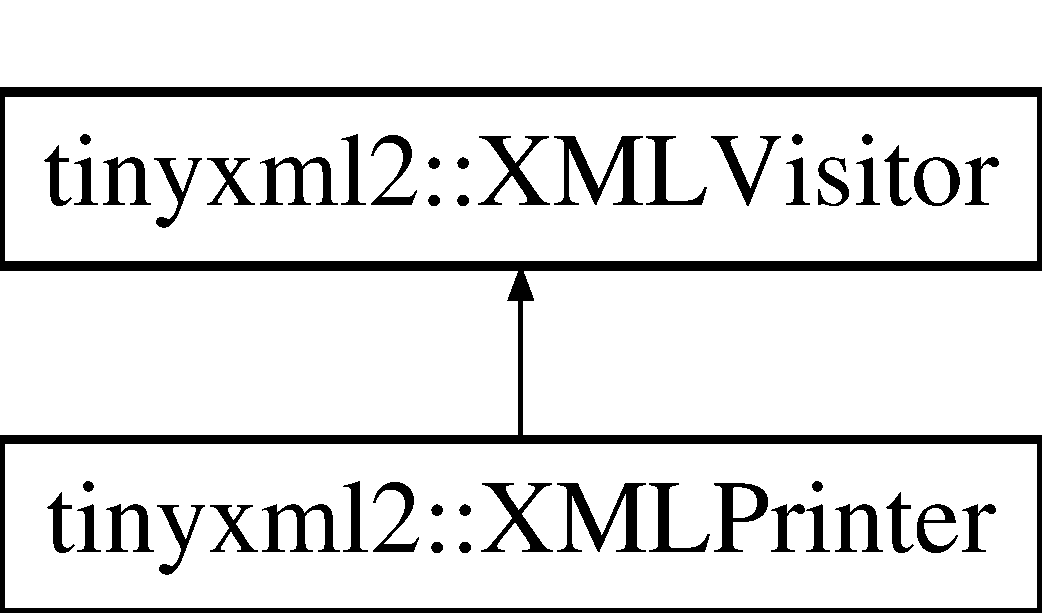
\includegraphics[height=2.000000cm]{classtinyxml2_1_1_x_m_l_printer}
\end{center}
\end{figure}
\subsection*{Public Member Functions}
\begin{DoxyCompactItemize}
\item 
\hyperlink{classtinyxml2_1_1_x_m_l_printer_aa6d3841c069085f5b8a27bc7103c04f7}{X\-M\-L\-Printer} (F\-I\-L\-E $\ast$file=0, bool compact=false, int depth=0)
\item 
\hyperlink{classtinyxml2_1_1_x_m_l_printer_a6de4c23a2941bd738a97b2bfd0000514}{$\sim$\-X\-M\-L\-Printer} ()
\item 
void \hyperlink{classtinyxml2_1_1_x_m_l_printer_a178c608ce8476043d5d6513819cde903}{Push\-Header} (bool write\-B\-O\-M, bool write\-Declaration)
\item 
void \hyperlink{classtinyxml2_1_1_x_m_l_printer_aa10d330818dbc31b44e9ffc27618bdfb}{Open\-Element} (const char $\ast$name)
\item 
void \hyperlink{classtinyxml2_1_1_x_m_l_printer_a9a4e2c9348b42e147629d5a99f4af3f0}{Push\-Attribute} (const char $\ast$name, const char $\ast$value)
\begin{DoxyCompactList}\small\item\em If streaming, add an attribute to an open element. \end{DoxyCompactList}\item 
void \hyperlink{classtinyxml2_1_1_x_m_l_printer_a69120c82088597372d28d0a98f2ee7a1}{Push\-Attribute} (const char $\ast$name, int value)
\item 
void \hyperlink{classtinyxml2_1_1_x_m_l_printer_aa41039e51990aaf5342f3e0575a692c4}{Push\-Attribute} (const char $\ast$name, unsigned value)
\item 
void \hyperlink{classtinyxml2_1_1_x_m_l_printer_a51f7950d7b7a19f0d3a0d549a318d45f}{Push\-Attribute} (const char $\ast$name, bool value)
\item 
void \hyperlink{classtinyxml2_1_1_x_m_l_printer_a1714867af40e68ca404c3e84b6cac2a6}{Push\-Attribute} (const char $\ast$name, double value)
\item 
void \hyperlink{classtinyxml2_1_1_x_m_l_printer_aed6cce4bd414a78b3e2a824803c3ec42}{Close\-Element} ()
\begin{DoxyCompactList}\small\item\em If streaming, close the Element. \end{DoxyCompactList}\item 
void \hyperlink{classtinyxml2_1_1_x_m_l_printer_a1cc16a9362df4332012cb13cff6441b3}{Push\-Text} (const char $\ast$text, bool cdata=false)
\begin{DoxyCompactList}\small\item\em Add a text node. \end{DoxyCompactList}\item 
void \hyperlink{classtinyxml2_1_1_x_m_l_printer_a3e0d4d78de25d4cf081009e1431cea7e}{Push\-Text} (int value)
\begin{DoxyCompactList}\small\item\em Add a text node from an integer. \end{DoxyCompactList}\item 
void \hyperlink{classtinyxml2_1_1_x_m_l_printer_a661fb50e7e0a4918d2d259cb0fae647e}{Push\-Text} (unsigned value)
\begin{DoxyCompactList}\small\item\em Add a text node from an unsigned. \end{DoxyCompactList}\item 
void \hyperlink{classtinyxml2_1_1_x_m_l_printer_a4390e5fa1ed05189a8686647345ab29f}{Push\-Text} (bool value)
\begin{DoxyCompactList}\small\item\em Add a text node from a bool. \end{DoxyCompactList}\item 
void \hyperlink{classtinyxml2_1_1_x_m_l_printer_a1dbb1390e829d0673af66b9cd1928bd7}{Push\-Text} (float value)
\begin{DoxyCompactList}\small\item\em Add a text node from a float. \end{DoxyCompactList}\item 
void \hyperlink{classtinyxml2_1_1_x_m_l_printer_aa715302dfc09473c77c853cbd5431965}{Push\-Text} (double value)
\begin{DoxyCompactList}\small\item\em Add a text node from a double. \end{DoxyCompactList}\item 
void \hyperlink{classtinyxml2_1_1_x_m_l_printer_afc8416814219591c2fd5656e0c233140}{Push\-Comment} (const char $\ast$comment)
\begin{DoxyCompactList}\small\item\em Add a comment. \end{DoxyCompactList}\item 
void \hyperlink{classtinyxml2_1_1_x_m_l_printer_a2fe3565e262594efc6c0276723c83fe7}{Push\-Declaration} (const char $\ast$value)
\item 
void \hyperlink{classtinyxml2_1_1_x_m_l_printer_ab1efc6d1548505e9984185f58f54b713}{Push\-Unknown} (const char $\ast$value)
\item 
virtual bool \hyperlink{classtinyxml2_1_1_x_m_l_printer_a9aa1de11a55a07db55a90fde37d7afad}{Visit\-Enter} (const \hyperlink{classtinyxml2_1_1_x_m_l_document}{X\-M\-L\-Document} \&)
\begin{DoxyCompactList}\small\item\em Visit a document. \end{DoxyCompactList}\item 
virtual bool \hyperlink{classtinyxml2_1_1_x_m_l_printer_a15fc1f2b922f540917dcf52808737b29}{Visit\-Exit} (const \hyperlink{classtinyxml2_1_1_x_m_l_document}{X\-M\-L\-Document} \&)
\begin{DoxyCompactList}\small\item\em Visit a document. \end{DoxyCompactList}\item 
virtual bool \hyperlink{classtinyxml2_1_1_x_m_l_printer_a169b2509d8eabb70811b2bb8cfd1f5d1}{Visit\-Enter} (const \hyperlink{classtinyxml2_1_1_x_m_l_element}{X\-M\-L\-Element} \&element, const \hyperlink{classtinyxml2_1_1_x_m_l_attribute}{X\-M\-L\-Attribute} $\ast$attribute)
\begin{DoxyCompactList}\small\item\em Visit an element. \end{DoxyCompactList}\item 
virtual bool \hyperlink{classtinyxml2_1_1_x_m_l_printer_a2edd48405971a88951c71c9df86a2f50}{Visit\-Exit} (const \hyperlink{classtinyxml2_1_1_x_m_l_element}{X\-M\-L\-Element} \&element)
\begin{DoxyCompactList}\small\item\em Visit an element. \end{DoxyCompactList}\item 
virtual bool \hyperlink{classtinyxml2_1_1_x_m_l_printer_adc0e42b4f6fcb90a95630c79575d030b}{Visit} (const \hyperlink{classtinyxml2_1_1_x_m_l_text}{X\-M\-L\-Text} \&text)
\begin{DoxyCompactList}\small\item\em Visit a text node. \end{DoxyCompactList}\item 
virtual bool \hyperlink{classtinyxml2_1_1_x_m_l_printer_aa294c5c01af0ebb9114902456e4cb53c}{Visit} (const \hyperlink{classtinyxml2_1_1_x_m_l_comment}{X\-M\-L\-Comment} \&comment)
\begin{DoxyCompactList}\small\item\em Visit a comment node. \end{DoxyCompactList}\item 
virtual bool \hyperlink{classtinyxml2_1_1_x_m_l_printer_acfc625b2549304b9c7eb85ebd5c5eb39}{Visit} (const \hyperlink{classtinyxml2_1_1_x_m_l_declaration}{X\-M\-L\-Declaration} \&declaration)
\begin{DoxyCompactList}\small\item\em Visit a declaration. \end{DoxyCompactList}\item 
virtual bool \hyperlink{classtinyxml2_1_1_x_m_l_printer_ab8af5455bbf9e4be2663e6642fcd7e32}{Visit} (const \hyperlink{classtinyxml2_1_1_x_m_l_unknown}{X\-M\-L\-Unknown} \&unknown)
\begin{DoxyCompactList}\small\item\em Visit an unknown node. \end{DoxyCompactList}\item 
const char $\ast$ \hyperlink{classtinyxml2_1_1_x_m_l_printer_a4a1b788e11b540921ec50687cd2b24a9}{C\-Str} () const 
\item 
int \hyperlink{classtinyxml2_1_1_x_m_l_printer_a02c3c5f8c6c007dcbaf10595d9e22bf0}{C\-Str\-Size} () const 
\end{DoxyCompactItemize}


\subsection{Detailed Description}
Printing functionality. The \hyperlink{classtinyxml2_1_1_x_m_l_printer}{X\-M\-L\-Printer} gives you more options than the \hyperlink{classtinyxml2_1_1_x_m_l_document_a686ea28672c0e0c60383ec28148c1ac0}{X\-M\-L\-Document\-::\-Print()} method.

It can\-:
\begin{DoxyEnumerate}
\item Print to memory.
\item Print to a file you provide.
\item Print X\-M\-L without a \hyperlink{classtinyxml2_1_1_x_m_l_document}{X\-M\-L\-Document}.
\end{DoxyEnumerate}

Print to Memory

\begin{DoxyVerb}XMLPrinter printer;
doc.Print( &printer );
SomeFunction( printer.CStr() );
\end{DoxyVerb}


Print to a File

You provide the file pointer. \begin{DoxyVerb}XMLPrinter printer( fp );
doc.Print( &printer );
\end{DoxyVerb}


Print without a \hyperlink{classtinyxml2_1_1_x_m_l_document}{X\-M\-L\-Document}

When loading, an X\-M\-L parser is very useful. However, sometimes when saving, it just gets in the way. The code is often set up for streaming, and constructing the D\-O\-M is just overhead.

The Printer supports the streaming case. The following code prints out a trivially simple X\-M\-L file without ever creating an X\-M\-L document.

\begin{DoxyVerb}XMLPrinter printer( fp );
printer.OpenElement( "foo" );
printer.PushAttribute( "foo", "bar" );
printer.CloseElement();
\end{DoxyVerb}
 

Definition at line 1877 of file tinyxml2.\-hpp.



\subsection{Constructor \& Destructor Documentation}
\hypertarget{classtinyxml2_1_1_x_m_l_printer_aa6d3841c069085f5b8a27bc7103c04f7}{\index{tinyxml2\-::\-X\-M\-L\-Printer@{tinyxml2\-::\-X\-M\-L\-Printer}!X\-M\-L\-Printer@{X\-M\-L\-Printer}}
\index{X\-M\-L\-Printer@{X\-M\-L\-Printer}!tinyxml2::XMLPrinter@{tinyxml2\-::\-X\-M\-L\-Printer}}
\subsubsection[{X\-M\-L\-Printer}]{\setlength{\rightskip}{0pt plus 5cm}tinyxml2\-::\-X\-M\-L\-Printer\-::\-X\-M\-L\-Printer (
\begin{DoxyParamCaption}
\item[{F\-I\-L\-E $\ast$}]{file = {\ttfamily 0}, }
\item[{bool}]{compact = {\ttfamily false}, }
\item[{int}]{depth = {\ttfamily 0}}
\end{DoxyParamCaption}
)}}\label{classtinyxml2_1_1_x_m_l_printer_aa6d3841c069085f5b8a27bc7103c04f7}
Construct the printer. If the F\-I\-L\-E$\ast$ is specified, this will print to the F\-I\-L\-E. Else it will print to memory, and the result is available in \hyperlink{classtinyxml2_1_1_x_m_l_printer_a4a1b788e11b540921ec50687cd2b24a9}{C\-Str()}. If 'compact' is set to true, then output is created with only required whitespace and newlines. 

Definition at line 1732 of file tinyxml2.\-cpp.

\hypertarget{classtinyxml2_1_1_x_m_l_printer_a6de4c23a2941bd738a97b2bfd0000514}{\index{tinyxml2\-::\-X\-M\-L\-Printer@{tinyxml2\-::\-X\-M\-L\-Printer}!$\sim$\-X\-M\-L\-Printer@{$\sim$\-X\-M\-L\-Printer}}
\index{$\sim$\-X\-M\-L\-Printer@{$\sim$\-X\-M\-L\-Printer}!tinyxml2::XMLPrinter@{tinyxml2\-::\-X\-M\-L\-Printer}}
\subsubsection[{$\sim$\-X\-M\-L\-Printer}]{\setlength{\rightskip}{0pt plus 5cm}tinyxml2\-::\-X\-M\-L\-Printer\-::$\sim$\-X\-M\-L\-Printer (
\begin{DoxyParamCaption}
{}
\end{DoxyParamCaption}
)\hspace{0.3cm}{\ttfamily [inline]}}}\label{classtinyxml2_1_1_x_m_l_printer_a6de4c23a2941bd738a97b2bfd0000514}


Definition at line 1887 of file tinyxml2.\-hpp.



\subsection{Member Function Documentation}
\hypertarget{classtinyxml2_1_1_x_m_l_printer_aed6cce4bd414a78b3e2a824803c3ec42}{\index{tinyxml2\-::\-X\-M\-L\-Printer@{tinyxml2\-::\-X\-M\-L\-Printer}!Close\-Element@{Close\-Element}}
\index{Close\-Element@{Close\-Element}!tinyxml2::XMLPrinter@{tinyxml2\-::\-X\-M\-L\-Printer}}
\subsubsection[{Close\-Element}]{\setlength{\rightskip}{0pt plus 5cm}void tinyxml2\-::\-X\-M\-L\-Printer\-::\-Close\-Element (
\begin{DoxyParamCaption}
{}
\end{DoxyParamCaption}
)}}\label{classtinyxml2_1_1_x_m_l_printer_aed6cce4bd414a78b3e2a824803c3ec42}


If streaming, close the Element. 



Definition at line 1914 of file tinyxml2.\-cpp.

\hypertarget{classtinyxml2_1_1_x_m_l_printer_a4a1b788e11b540921ec50687cd2b24a9}{\index{tinyxml2\-::\-X\-M\-L\-Printer@{tinyxml2\-::\-X\-M\-L\-Printer}!C\-Str@{C\-Str}}
\index{C\-Str@{C\-Str}!tinyxml2::XMLPrinter@{tinyxml2\-::\-X\-M\-L\-Printer}}
\subsubsection[{C\-Str}]{\setlength{\rightskip}{0pt plus 5cm}const char$\ast$ tinyxml2\-::\-X\-M\-L\-Printer\-::\-C\-Str (
\begin{DoxyParamCaption}
{}
\end{DoxyParamCaption}
) const\hspace{0.3cm}{\ttfamily [inline]}}}\label{classtinyxml2_1_1_x_m_l_printer_a4a1b788e11b540921ec50687cd2b24a9}
If in print to memory mode, return a pointer to the X\-M\-L file in memory. 

Definition at line 1940 of file tinyxml2.\-hpp.

\hypertarget{classtinyxml2_1_1_x_m_l_printer_a02c3c5f8c6c007dcbaf10595d9e22bf0}{\index{tinyxml2\-::\-X\-M\-L\-Printer@{tinyxml2\-::\-X\-M\-L\-Printer}!C\-Str\-Size@{C\-Str\-Size}}
\index{C\-Str\-Size@{C\-Str\-Size}!tinyxml2::XMLPrinter@{tinyxml2\-::\-X\-M\-L\-Printer}}
\subsubsection[{C\-Str\-Size}]{\setlength{\rightskip}{0pt plus 5cm}int tinyxml2\-::\-X\-M\-L\-Printer\-::\-C\-Str\-Size (
\begin{DoxyParamCaption}
{}
\end{DoxyParamCaption}
) const\hspace{0.3cm}{\ttfamily [inline]}}}\label{classtinyxml2_1_1_x_m_l_printer_a02c3c5f8c6c007dcbaf10595d9e22bf0}
If in print to memory mode, return the size of the X\-M\-L file in memory. (Note the size returned includes the terminating null.) 

Definition at line 1948 of file tinyxml2.\-hpp.

\hypertarget{classtinyxml2_1_1_x_m_l_printer_aa10d330818dbc31b44e9ffc27618bdfb}{\index{tinyxml2\-::\-X\-M\-L\-Printer@{tinyxml2\-::\-X\-M\-L\-Printer}!Open\-Element@{Open\-Element}}
\index{Open\-Element@{Open\-Element}!tinyxml2::XMLPrinter@{tinyxml2\-::\-X\-M\-L\-Printer}}
\subsubsection[{Open\-Element}]{\setlength{\rightskip}{0pt plus 5cm}void tinyxml2\-::\-X\-M\-L\-Printer\-::\-Open\-Element (
\begin{DoxyParamCaption}
\item[{const char $\ast$}]{name}
\end{DoxyParamCaption}
)}}\label{classtinyxml2_1_1_x_m_l_printer_aa10d330818dbc31b44e9ffc27618bdfb}
If streaming, start writing an element. The element must be closed with \hyperlink{classtinyxml2_1_1_x_m_l_printer_aed6cce4bd414a78b3e2a824803c3ec42}{Close\-Element()} 

Definition at line 1852 of file tinyxml2.\-cpp.

\hypertarget{classtinyxml2_1_1_x_m_l_printer_a9a4e2c9348b42e147629d5a99f4af3f0}{\index{tinyxml2\-::\-X\-M\-L\-Printer@{tinyxml2\-::\-X\-M\-L\-Printer}!Push\-Attribute@{Push\-Attribute}}
\index{Push\-Attribute@{Push\-Attribute}!tinyxml2::XMLPrinter@{tinyxml2\-::\-X\-M\-L\-Printer}}
\subsubsection[{Push\-Attribute}]{\setlength{\rightskip}{0pt plus 5cm}void tinyxml2\-::\-X\-M\-L\-Printer\-::\-Push\-Attribute (
\begin{DoxyParamCaption}
\item[{const char $\ast$}]{name, }
\item[{const char $\ast$}]{value}
\end{DoxyParamCaption}
)}}\label{classtinyxml2_1_1_x_m_l_printer_a9a4e2c9348b42e147629d5a99f4af3f0}


If streaming, add an attribute to an open element. 



Definition at line 1873 of file tinyxml2.\-cpp.

\hypertarget{classtinyxml2_1_1_x_m_l_printer_a69120c82088597372d28d0a98f2ee7a1}{\index{tinyxml2\-::\-X\-M\-L\-Printer@{tinyxml2\-::\-X\-M\-L\-Printer}!Push\-Attribute@{Push\-Attribute}}
\index{Push\-Attribute@{Push\-Attribute}!tinyxml2::XMLPrinter@{tinyxml2\-::\-X\-M\-L\-Printer}}
\subsubsection[{Push\-Attribute}]{\setlength{\rightskip}{0pt plus 5cm}void tinyxml2\-::\-X\-M\-L\-Printer\-::\-Push\-Attribute (
\begin{DoxyParamCaption}
\item[{const char $\ast$}]{name, }
\item[{int}]{value}
\end{DoxyParamCaption}
)}}\label{classtinyxml2_1_1_x_m_l_printer_a69120c82088597372d28d0a98f2ee7a1}


Definition at line 1882 of file tinyxml2.\-cpp.

\hypertarget{classtinyxml2_1_1_x_m_l_printer_aa41039e51990aaf5342f3e0575a692c4}{\index{tinyxml2\-::\-X\-M\-L\-Printer@{tinyxml2\-::\-X\-M\-L\-Printer}!Push\-Attribute@{Push\-Attribute}}
\index{Push\-Attribute@{Push\-Attribute}!tinyxml2::XMLPrinter@{tinyxml2\-::\-X\-M\-L\-Printer}}
\subsubsection[{Push\-Attribute}]{\setlength{\rightskip}{0pt plus 5cm}void tinyxml2\-::\-X\-M\-L\-Printer\-::\-Push\-Attribute (
\begin{DoxyParamCaption}
\item[{const char $\ast$}]{name, }
\item[{unsigned}]{value}
\end{DoxyParamCaption}
)}}\label{classtinyxml2_1_1_x_m_l_printer_aa41039e51990aaf5342f3e0575a692c4}


Definition at line 1890 of file tinyxml2.\-cpp.

\hypertarget{classtinyxml2_1_1_x_m_l_printer_a51f7950d7b7a19f0d3a0d549a318d45f}{\index{tinyxml2\-::\-X\-M\-L\-Printer@{tinyxml2\-::\-X\-M\-L\-Printer}!Push\-Attribute@{Push\-Attribute}}
\index{Push\-Attribute@{Push\-Attribute}!tinyxml2::XMLPrinter@{tinyxml2\-::\-X\-M\-L\-Printer}}
\subsubsection[{Push\-Attribute}]{\setlength{\rightskip}{0pt plus 5cm}void tinyxml2\-::\-X\-M\-L\-Printer\-::\-Push\-Attribute (
\begin{DoxyParamCaption}
\item[{const char $\ast$}]{name, }
\item[{bool}]{value}
\end{DoxyParamCaption}
)}}\label{classtinyxml2_1_1_x_m_l_printer_a51f7950d7b7a19f0d3a0d549a318d45f}


Definition at line 1898 of file tinyxml2.\-cpp.

\hypertarget{classtinyxml2_1_1_x_m_l_printer_a1714867af40e68ca404c3e84b6cac2a6}{\index{tinyxml2\-::\-X\-M\-L\-Printer@{tinyxml2\-::\-X\-M\-L\-Printer}!Push\-Attribute@{Push\-Attribute}}
\index{Push\-Attribute@{Push\-Attribute}!tinyxml2::XMLPrinter@{tinyxml2\-::\-X\-M\-L\-Printer}}
\subsubsection[{Push\-Attribute}]{\setlength{\rightskip}{0pt plus 5cm}void tinyxml2\-::\-X\-M\-L\-Printer\-::\-Push\-Attribute (
\begin{DoxyParamCaption}
\item[{const char $\ast$}]{name, }
\item[{double}]{value}
\end{DoxyParamCaption}
)}}\label{classtinyxml2_1_1_x_m_l_printer_a1714867af40e68ca404c3e84b6cac2a6}


Definition at line 1906 of file tinyxml2.\-cpp.

\hypertarget{classtinyxml2_1_1_x_m_l_printer_afc8416814219591c2fd5656e0c233140}{\index{tinyxml2\-::\-X\-M\-L\-Printer@{tinyxml2\-::\-X\-M\-L\-Printer}!Push\-Comment@{Push\-Comment}}
\index{Push\-Comment@{Push\-Comment}!tinyxml2::XMLPrinter@{tinyxml2\-::\-X\-M\-L\-Printer}}
\subsubsection[{Push\-Comment}]{\setlength{\rightskip}{0pt plus 5cm}void tinyxml2\-::\-X\-M\-L\-Printer\-::\-Push\-Comment (
\begin{DoxyParamCaption}
\item[{const char $\ast$}]{comment}
\end{DoxyParamCaption}
)}}\label{classtinyxml2_1_1_x_m_l_printer_afc8416814219591c2fd5656e0c233140}


Add a comment. 



Definition at line 2004 of file tinyxml2.\-cpp.

\hypertarget{classtinyxml2_1_1_x_m_l_printer_a2fe3565e262594efc6c0276723c83fe7}{\index{tinyxml2\-::\-X\-M\-L\-Printer@{tinyxml2\-::\-X\-M\-L\-Printer}!Push\-Declaration@{Push\-Declaration}}
\index{Push\-Declaration@{Push\-Declaration}!tinyxml2::XMLPrinter@{tinyxml2\-::\-X\-M\-L\-Printer}}
\subsubsection[{Push\-Declaration}]{\setlength{\rightskip}{0pt plus 5cm}void tinyxml2\-::\-X\-M\-L\-Printer\-::\-Push\-Declaration (
\begin{DoxyParamCaption}
\item[{const char $\ast$}]{value}
\end{DoxyParamCaption}
)}}\label{classtinyxml2_1_1_x_m_l_printer_a2fe3565e262594efc6c0276723c83fe7}


Definition at line 2018 of file tinyxml2.\-cpp.

\hypertarget{classtinyxml2_1_1_x_m_l_printer_a178c608ce8476043d5d6513819cde903}{\index{tinyxml2\-::\-X\-M\-L\-Printer@{tinyxml2\-::\-X\-M\-L\-Printer}!Push\-Header@{Push\-Header}}
\index{Push\-Header@{Push\-Header}!tinyxml2::XMLPrinter@{tinyxml2\-::\-X\-M\-L\-Printer}}
\subsubsection[{Push\-Header}]{\setlength{\rightskip}{0pt plus 5cm}void tinyxml2\-::\-X\-M\-L\-Printer\-::\-Push\-Header (
\begin{DoxyParamCaption}
\item[{bool}]{write\-B\-O\-M, }
\item[{bool}]{write\-Declaration}
\end{DoxyParamCaption}
)}}\label{classtinyxml2_1_1_x_m_l_printer_a178c608ce8476043d5d6513819cde903}
If streaming, write the B\-O\-M and declaration. 

Definition at line 1840 of file tinyxml2.\-cpp.

\hypertarget{classtinyxml2_1_1_x_m_l_printer_a1cc16a9362df4332012cb13cff6441b3}{\index{tinyxml2\-::\-X\-M\-L\-Printer@{tinyxml2\-::\-X\-M\-L\-Printer}!Push\-Text@{Push\-Text}}
\index{Push\-Text@{Push\-Text}!tinyxml2::XMLPrinter@{tinyxml2\-::\-X\-M\-L\-Printer}}
\subsubsection[{Push\-Text}]{\setlength{\rightskip}{0pt plus 5cm}void tinyxml2\-::\-X\-M\-L\-Printer\-::\-Push\-Text (
\begin{DoxyParamCaption}
\item[{const char $\ast$}]{text, }
\item[{bool}]{cdata = {\ttfamily false}}
\end{DoxyParamCaption}
)}}\label{classtinyxml2_1_1_x_m_l_printer_a1cc16a9362df4332012cb13cff6441b3}


Add a text node. 



Definition at line 1947 of file tinyxml2.\-cpp.

\hypertarget{classtinyxml2_1_1_x_m_l_printer_a3e0d4d78de25d4cf081009e1431cea7e}{\index{tinyxml2\-::\-X\-M\-L\-Printer@{tinyxml2\-::\-X\-M\-L\-Printer}!Push\-Text@{Push\-Text}}
\index{Push\-Text@{Push\-Text}!tinyxml2::XMLPrinter@{tinyxml2\-::\-X\-M\-L\-Printer}}
\subsubsection[{Push\-Text}]{\setlength{\rightskip}{0pt plus 5cm}void tinyxml2\-::\-X\-M\-L\-Printer\-::\-Push\-Text (
\begin{DoxyParamCaption}
\item[{int}]{value}
\end{DoxyParamCaption}
)}}\label{classtinyxml2_1_1_x_m_l_printer_a3e0d4d78de25d4cf081009e1431cea7e}


Add a text node from an integer. 



Definition at line 1964 of file tinyxml2.\-cpp.

\hypertarget{classtinyxml2_1_1_x_m_l_printer_a661fb50e7e0a4918d2d259cb0fae647e}{\index{tinyxml2\-::\-X\-M\-L\-Printer@{tinyxml2\-::\-X\-M\-L\-Printer}!Push\-Text@{Push\-Text}}
\index{Push\-Text@{Push\-Text}!tinyxml2::XMLPrinter@{tinyxml2\-::\-X\-M\-L\-Printer}}
\subsubsection[{Push\-Text}]{\setlength{\rightskip}{0pt plus 5cm}void tinyxml2\-::\-X\-M\-L\-Printer\-::\-Push\-Text (
\begin{DoxyParamCaption}
\item[{unsigned}]{value}
\end{DoxyParamCaption}
)}}\label{classtinyxml2_1_1_x_m_l_printer_a661fb50e7e0a4918d2d259cb0fae647e}


Add a text node from an unsigned. 



Definition at line 1972 of file tinyxml2.\-cpp.

\hypertarget{classtinyxml2_1_1_x_m_l_printer_a4390e5fa1ed05189a8686647345ab29f}{\index{tinyxml2\-::\-X\-M\-L\-Printer@{tinyxml2\-::\-X\-M\-L\-Printer}!Push\-Text@{Push\-Text}}
\index{Push\-Text@{Push\-Text}!tinyxml2::XMLPrinter@{tinyxml2\-::\-X\-M\-L\-Printer}}
\subsubsection[{Push\-Text}]{\setlength{\rightskip}{0pt plus 5cm}void tinyxml2\-::\-X\-M\-L\-Printer\-::\-Push\-Text (
\begin{DoxyParamCaption}
\item[{bool}]{value}
\end{DoxyParamCaption}
)}}\label{classtinyxml2_1_1_x_m_l_printer_a4390e5fa1ed05189a8686647345ab29f}


Add a text node from a bool. 



Definition at line 1980 of file tinyxml2.\-cpp.

\hypertarget{classtinyxml2_1_1_x_m_l_printer_a1dbb1390e829d0673af66b9cd1928bd7}{\index{tinyxml2\-::\-X\-M\-L\-Printer@{tinyxml2\-::\-X\-M\-L\-Printer}!Push\-Text@{Push\-Text}}
\index{Push\-Text@{Push\-Text}!tinyxml2::XMLPrinter@{tinyxml2\-::\-X\-M\-L\-Printer}}
\subsubsection[{Push\-Text}]{\setlength{\rightskip}{0pt plus 5cm}void tinyxml2\-::\-X\-M\-L\-Printer\-::\-Push\-Text (
\begin{DoxyParamCaption}
\item[{float}]{value}
\end{DoxyParamCaption}
)}}\label{classtinyxml2_1_1_x_m_l_printer_a1dbb1390e829d0673af66b9cd1928bd7}


Add a text node from a float. 



Definition at line 1988 of file tinyxml2.\-cpp.

\hypertarget{classtinyxml2_1_1_x_m_l_printer_aa715302dfc09473c77c853cbd5431965}{\index{tinyxml2\-::\-X\-M\-L\-Printer@{tinyxml2\-::\-X\-M\-L\-Printer}!Push\-Text@{Push\-Text}}
\index{Push\-Text@{Push\-Text}!tinyxml2::XMLPrinter@{tinyxml2\-::\-X\-M\-L\-Printer}}
\subsubsection[{Push\-Text}]{\setlength{\rightskip}{0pt plus 5cm}void tinyxml2\-::\-X\-M\-L\-Printer\-::\-Push\-Text (
\begin{DoxyParamCaption}
\item[{double}]{value}
\end{DoxyParamCaption}
)}}\label{classtinyxml2_1_1_x_m_l_printer_aa715302dfc09473c77c853cbd5431965}


Add a text node from a double. 



Definition at line 1996 of file tinyxml2.\-cpp.

\hypertarget{classtinyxml2_1_1_x_m_l_printer_ab1efc6d1548505e9984185f58f54b713}{\index{tinyxml2\-::\-X\-M\-L\-Printer@{tinyxml2\-::\-X\-M\-L\-Printer}!Push\-Unknown@{Push\-Unknown}}
\index{Push\-Unknown@{Push\-Unknown}!tinyxml2::XMLPrinter@{tinyxml2\-::\-X\-M\-L\-Printer}}
\subsubsection[{Push\-Unknown}]{\setlength{\rightskip}{0pt plus 5cm}void tinyxml2\-::\-X\-M\-L\-Printer\-::\-Push\-Unknown (
\begin{DoxyParamCaption}
\item[{const char $\ast$}]{value}
\end{DoxyParamCaption}
)}}\label{classtinyxml2_1_1_x_m_l_printer_ab1efc6d1548505e9984185f58f54b713}


Definition at line 2032 of file tinyxml2.\-cpp.

\hypertarget{classtinyxml2_1_1_x_m_l_printer_adc0e42b4f6fcb90a95630c79575d030b}{\index{tinyxml2\-::\-X\-M\-L\-Printer@{tinyxml2\-::\-X\-M\-L\-Printer}!Visit@{Visit}}
\index{Visit@{Visit}!tinyxml2::XMLPrinter@{tinyxml2\-::\-X\-M\-L\-Printer}}
\subsubsection[{Visit}]{\setlength{\rightskip}{0pt plus 5cm}bool tinyxml2\-::\-X\-M\-L\-Printer\-::\-Visit (
\begin{DoxyParamCaption}
\item[{const {\bf X\-M\-L\-Text} \&}]{}
\end{DoxyParamCaption}
)\hspace{0.3cm}{\ttfamily [virtual]}}}\label{classtinyxml2_1_1_x_m_l_printer_adc0e42b4f6fcb90a95630c79575d030b}


Visit a text node. 



Reimplemented from \hyperlink{classtinyxml2_1_1_x_m_l_visitor_af30233565856480ea48b6fa0d6dec65b}{tinyxml2\-::\-X\-M\-L\-Visitor}.



Definition at line 2074 of file tinyxml2.\-cpp.

\hypertarget{classtinyxml2_1_1_x_m_l_printer_aa294c5c01af0ebb9114902456e4cb53c}{\index{tinyxml2\-::\-X\-M\-L\-Printer@{tinyxml2\-::\-X\-M\-L\-Printer}!Visit@{Visit}}
\index{Visit@{Visit}!tinyxml2::XMLPrinter@{tinyxml2\-::\-X\-M\-L\-Printer}}
\subsubsection[{Visit}]{\setlength{\rightskip}{0pt plus 5cm}bool tinyxml2\-::\-X\-M\-L\-Printer\-::\-Visit (
\begin{DoxyParamCaption}
\item[{const {\bf X\-M\-L\-Comment} \&}]{}
\end{DoxyParamCaption}
)\hspace{0.3cm}{\ttfamily [virtual]}}}\label{classtinyxml2_1_1_x_m_l_printer_aa294c5c01af0ebb9114902456e4cb53c}


Visit a comment node. 



Reimplemented from \hyperlink{classtinyxml2_1_1_x_m_l_visitor_acc8147fb5a85f6c65721654e427752d7}{tinyxml2\-::\-X\-M\-L\-Visitor}.



Definition at line 2081 of file tinyxml2.\-cpp.

\hypertarget{classtinyxml2_1_1_x_m_l_printer_acfc625b2549304b9c7eb85ebd5c5eb39}{\index{tinyxml2\-::\-X\-M\-L\-Printer@{tinyxml2\-::\-X\-M\-L\-Printer}!Visit@{Visit}}
\index{Visit@{Visit}!tinyxml2::XMLPrinter@{tinyxml2\-::\-X\-M\-L\-Printer}}
\subsubsection[{Visit}]{\setlength{\rightskip}{0pt plus 5cm}bool tinyxml2\-::\-X\-M\-L\-Printer\-::\-Visit (
\begin{DoxyParamCaption}
\item[{const {\bf X\-M\-L\-Declaration} \&}]{}
\end{DoxyParamCaption}
)\hspace{0.3cm}{\ttfamily [virtual]}}}\label{classtinyxml2_1_1_x_m_l_printer_acfc625b2549304b9c7eb85ebd5c5eb39}


Visit a declaration. 



Reimplemented from \hyperlink{classtinyxml2_1_1_x_m_l_visitor_adc75bd459fc7ba8223b50f0616767f9a}{tinyxml2\-::\-X\-M\-L\-Visitor}.



Definition at line 2087 of file tinyxml2.\-cpp.

\hypertarget{classtinyxml2_1_1_x_m_l_printer_ab8af5455bbf9e4be2663e6642fcd7e32}{\index{tinyxml2\-::\-X\-M\-L\-Printer@{tinyxml2\-::\-X\-M\-L\-Printer}!Visit@{Visit}}
\index{Visit@{Visit}!tinyxml2::XMLPrinter@{tinyxml2\-::\-X\-M\-L\-Printer}}
\subsubsection[{Visit}]{\setlength{\rightskip}{0pt plus 5cm}bool tinyxml2\-::\-X\-M\-L\-Printer\-::\-Visit (
\begin{DoxyParamCaption}
\item[{const {\bf X\-M\-L\-Unknown} \&}]{}
\end{DoxyParamCaption}
)\hspace{0.3cm}{\ttfamily [virtual]}}}\label{classtinyxml2_1_1_x_m_l_printer_ab8af5455bbf9e4be2663e6642fcd7e32}


Visit an unknown node. 



Reimplemented from \hyperlink{classtinyxml2_1_1_x_m_l_visitor_a14e4748387c34bf53d24e8119bb1f292}{tinyxml2\-::\-X\-M\-L\-Visitor}.



Definition at line 2094 of file tinyxml2.\-cpp.

\hypertarget{classtinyxml2_1_1_x_m_l_printer_a9aa1de11a55a07db55a90fde37d7afad}{\index{tinyxml2\-::\-X\-M\-L\-Printer@{tinyxml2\-::\-X\-M\-L\-Printer}!Visit\-Enter@{Visit\-Enter}}
\index{Visit\-Enter@{Visit\-Enter}!tinyxml2::XMLPrinter@{tinyxml2\-::\-X\-M\-L\-Printer}}
\subsubsection[{Visit\-Enter}]{\setlength{\rightskip}{0pt plus 5cm}bool tinyxml2\-::\-X\-M\-L\-Printer\-::\-Visit\-Enter (
\begin{DoxyParamCaption}
\item[{const {\bf X\-M\-L\-Document} \&}]{}
\end{DoxyParamCaption}
)\hspace{0.3cm}{\ttfamily [virtual]}}}\label{classtinyxml2_1_1_x_m_l_printer_a9aa1de11a55a07db55a90fde37d7afad}


Visit a document. 



Reimplemented from \hyperlink{classtinyxml2_1_1_x_m_l_visitor_acb3c22fc5f60eb9db98f533f2761f67d}{tinyxml2\-::\-X\-M\-L\-Visitor}.



Definition at line 2046 of file tinyxml2.\-cpp.

\hypertarget{classtinyxml2_1_1_x_m_l_printer_a169b2509d8eabb70811b2bb8cfd1f5d1}{\index{tinyxml2\-::\-X\-M\-L\-Printer@{tinyxml2\-::\-X\-M\-L\-Printer}!Visit\-Enter@{Visit\-Enter}}
\index{Visit\-Enter@{Visit\-Enter}!tinyxml2::XMLPrinter@{tinyxml2\-::\-X\-M\-L\-Printer}}
\subsubsection[{Visit\-Enter}]{\setlength{\rightskip}{0pt plus 5cm}bool tinyxml2\-::\-X\-M\-L\-Printer\-::\-Visit\-Enter (
\begin{DoxyParamCaption}
\item[{const {\bf X\-M\-L\-Element} \&}]{, }
\item[{const {\bf X\-M\-L\-Attribute} $\ast$}]{}
\end{DoxyParamCaption}
)\hspace{0.3cm}{\ttfamily [virtual]}}}\label{classtinyxml2_1_1_x_m_l_printer_a169b2509d8eabb70811b2bb8cfd1f5d1}


Visit an element. 



Reimplemented from \hyperlink{classtinyxml2_1_1_x_m_l_visitor_af97980a17dd4e37448b181f5ddfa92b5}{tinyxml2\-::\-X\-M\-L\-Visitor}.



Definition at line 2056 of file tinyxml2.\-cpp.

\hypertarget{classtinyxml2_1_1_x_m_l_printer_a15fc1f2b922f540917dcf52808737b29}{\index{tinyxml2\-::\-X\-M\-L\-Printer@{tinyxml2\-::\-X\-M\-L\-Printer}!Visit\-Exit@{Visit\-Exit}}
\index{Visit\-Exit@{Visit\-Exit}!tinyxml2::XMLPrinter@{tinyxml2\-::\-X\-M\-L\-Printer}}
\subsubsection[{Visit\-Exit}]{\setlength{\rightskip}{0pt plus 5cm}virtual bool tinyxml2\-::\-X\-M\-L\-Printer\-::\-Visit\-Exit (
\begin{DoxyParamCaption}
\item[{const {\bf X\-M\-L\-Document} \&}]{}
\end{DoxyParamCaption}
)\hspace{0.3cm}{\ttfamily [inline]}, {\ttfamily [virtual]}}}\label{classtinyxml2_1_1_x_m_l_printer_a15fc1f2b922f540917dcf52808737b29}


Visit a document. 



Reimplemented from \hyperlink{classtinyxml2_1_1_x_m_l_visitor_a170e9989cd046ba904f302d087e07086}{tinyxml2\-::\-X\-M\-L\-Visitor}.



Definition at line 1924 of file tinyxml2.\-hpp.

\hypertarget{classtinyxml2_1_1_x_m_l_printer_a2edd48405971a88951c71c9df86a2f50}{\index{tinyxml2\-::\-X\-M\-L\-Printer@{tinyxml2\-::\-X\-M\-L\-Printer}!Visit\-Exit@{Visit\-Exit}}
\index{Visit\-Exit@{Visit\-Exit}!tinyxml2::XMLPrinter@{tinyxml2\-::\-X\-M\-L\-Printer}}
\subsubsection[{Visit\-Exit}]{\setlength{\rightskip}{0pt plus 5cm}bool tinyxml2\-::\-X\-M\-L\-Printer\-::\-Visit\-Exit (
\begin{DoxyParamCaption}
\item[{const {\bf X\-M\-L\-Element} \&}]{}
\end{DoxyParamCaption}
)\hspace{0.3cm}{\ttfamily [virtual]}}}\label{classtinyxml2_1_1_x_m_l_printer_a2edd48405971a88951c71c9df86a2f50}


Visit an element. 



Reimplemented from \hyperlink{classtinyxml2_1_1_x_m_l_visitor_a772f10ddc83f881956d32628faa16eb6}{tinyxml2\-::\-X\-M\-L\-Visitor}.



Definition at line 2067 of file tinyxml2.\-cpp.



The documentation for this class was generated from the following files\-:\begin{DoxyCompactItemize}
\item 
/home/lee/\-Projects/\-Sudden\-Awakening/\-Source/\hyperlink{tinyxml2_8hpp}{tinyxml2.\-hpp}\item 
/home/lee/\-Projects/\-Sudden\-Awakening/\-Source/\hyperlink{tinyxml2_8cpp}{tinyxml2.\-cpp}\end{DoxyCompactItemize}

\hypertarget{classtinyxml2_1_1_x_m_l_text}{\section{tinyxml2\-:\-:X\-M\-L\-Text Class Reference}
\label{classtinyxml2_1_1_x_m_l_text}\index{tinyxml2\-::\-X\-M\-L\-Text@{tinyxml2\-::\-X\-M\-L\-Text}}
}


{\ttfamily \#include $<$tinyxml2.\-hpp$>$}

Inheritance diagram for tinyxml2\-:\-:X\-M\-L\-Text\-:\begin{figure}[H]
\begin{center}
\leavevmode
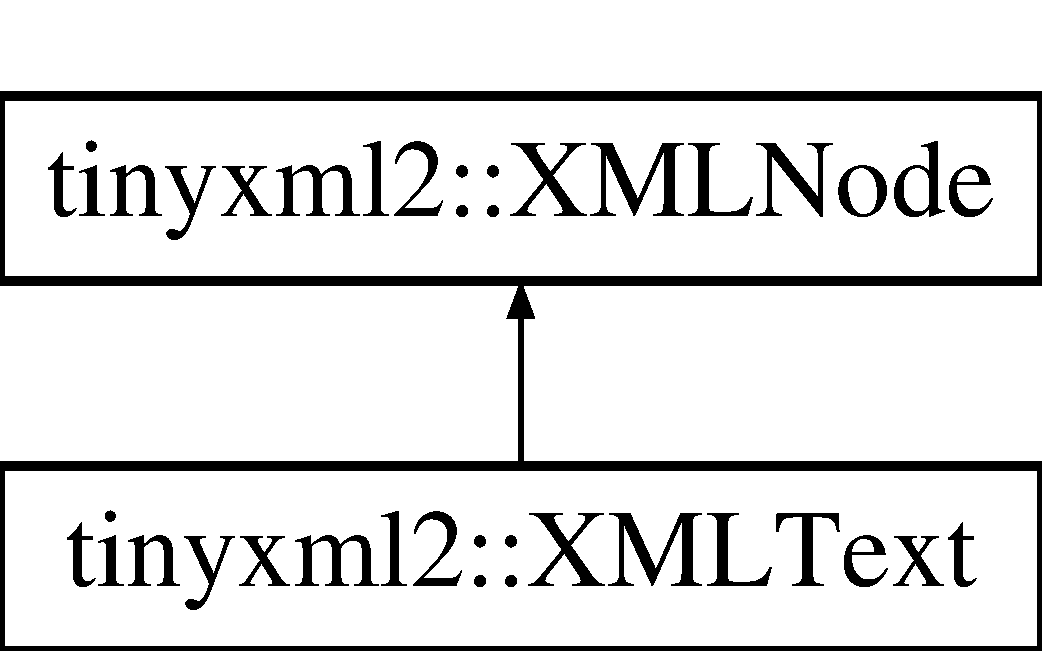
\includegraphics[height=2.000000cm]{classtinyxml2_1_1_x_m_l_text}
\end{center}
\end{figure}
\subsection*{Public Member Functions}
\begin{DoxyCompactItemize}
\item 
virtual bool \hyperlink{classtinyxml2_1_1_x_m_l_text_ae659d4fc7351a7df11c111cbe1ade46f}{Accept} (\hyperlink{classtinyxml2_1_1_x_m_l_visitor}{X\-M\-L\-Visitor} $\ast$visitor) const 
\item 
virtual \hyperlink{classtinyxml2_1_1_x_m_l_text}{X\-M\-L\-Text} $\ast$ \hyperlink{classtinyxml2_1_1_x_m_l_text_ab1213b4ddebe9b17ec7e7040e9f1caf7}{To\-Text} ()
\begin{DoxyCompactList}\small\item\em Safely cast to Text, or null. \end{DoxyCompactList}\item 
virtual const \hyperlink{classtinyxml2_1_1_x_m_l_text}{X\-M\-L\-Text} $\ast$ \hyperlink{classtinyxml2_1_1_x_m_l_text_a1e53cbc60968fe966790a65eaf87baaa}{To\-Text} () const 
\item 
void \hyperlink{classtinyxml2_1_1_x_m_l_text_ad080357d76ab7cc59d7651249949329d}{Set\-C\-Data} (bool is\-C\-Data)
\begin{DoxyCompactList}\small\item\em Declare whether this should be C\-D\-A\-T\-A or standard text. \end{DoxyCompactList}\item 
bool \hyperlink{classtinyxml2_1_1_x_m_l_text_a125574fe49da80efbae1349f20d02d41}{C\-Data} () const 
\begin{DoxyCompactList}\small\item\em Returns true if this is a C\-D\-A\-T\-A text element. \end{DoxyCompactList}\item 
char $\ast$ \hyperlink{classtinyxml2_1_1_x_m_l_text_ac18d9eec9f12b827b0d02b0847bf279e}{Parse\-Deep} (char $\ast$, \hyperlink{classtinyxml2_1_1_str_pair}{Str\-Pair} $\ast$end\-Tag)
\item 
virtual \hyperlink{classtinyxml2_1_1_x_m_l_node}{X\-M\-L\-Node} $\ast$ \hyperlink{classtinyxml2_1_1_x_m_l_text_af5115f8cc83de2947ed6a9d13e2f88c8}{Shallow\-Clone} (\hyperlink{classtinyxml2_1_1_x_m_l_document}{X\-M\-L\-Document} $\ast$document) const 
\item 
virtual bool \hyperlink{classtinyxml2_1_1_x_m_l_text_a1588aa5d23cb21eb31f36df0aaaa8d66}{Shallow\-Equal} (const \hyperlink{classtinyxml2_1_1_x_m_l_node}{X\-M\-L\-Node} $\ast$compare) const 
\end{DoxyCompactItemize}
\subsection*{Protected Member Functions}
\begin{DoxyCompactItemize}
\item 
\hyperlink{classtinyxml2_1_1_x_m_l_text_ad9f46d70e61e5386ead93728d8b90267}{X\-M\-L\-Text} (\hyperlink{classtinyxml2_1_1_x_m_l_document}{X\-M\-L\-Document} $\ast$doc)
\item 
virtual \hyperlink{classtinyxml2_1_1_x_m_l_text_ae9b8790d0dc13914394dbd7437c0e59d}{$\sim$\-X\-M\-L\-Text} ()
\item 
\hyperlink{classtinyxml2_1_1_x_m_l_text_a002156e1f61ee6d48e5368b7cca25582}{X\-M\-L\-Text} (const \hyperlink{classtinyxml2_1_1_x_m_l_text}{X\-M\-L\-Text} \&)
\item 
\hyperlink{classtinyxml2_1_1_x_m_l_text}{X\-M\-L\-Text} \& \hyperlink{classtinyxml2_1_1_x_m_l_text_ad8c9f398d92fa472e213b89d8483ae8f}{operator=} (const \hyperlink{classtinyxml2_1_1_x_m_l_text}{X\-M\-L\-Text} \&)
\end{DoxyCompactItemize}
\subsection*{Friends}
\begin{DoxyCompactItemize}
\item 
class \hyperlink{classtinyxml2_1_1_x_m_l_text_a449202cfc89e7ae5c2f81995476f9ec1}{X\-M\-L\-Base}
\item 
class \hyperlink{classtinyxml2_1_1_x_m_l_text_a4eee3bda60c60a30e4e8cd4ea91c4c6e}{X\-M\-L\-Document}
\end{DoxyCompactItemize}
\subsection*{Additional Inherited Members}


\subsection{Detailed Description}
X\-M\-L text.

Note that a text node can have child element nodes, for example\-: \begin{DoxyVerb}<root>This is <b>bold</b></root>
\end{DoxyVerb}


A text node can have 2 ways to output the next. \char`\"{}normal\char`\"{} output and C\-D\-A\-T\-A. It will default to the mode it was parsed from the X\-M\-L file and you generally want to leave it alone, but you can change the output mode with \hyperlink{classtinyxml2_1_1_x_m_l_text_ad080357d76ab7cc59d7651249949329d}{Set\-C\-Data()} and query it with \hyperlink{classtinyxml2_1_1_x_m_l_text_a125574fe49da80efbae1349f20d02d41}{C\-Data()}. 

Definition at line 839 of file tinyxml2.\-hpp.



\subsection{Constructor \& Destructor Documentation}
\hypertarget{classtinyxml2_1_1_x_m_l_text_ad9f46d70e61e5386ead93728d8b90267}{\index{tinyxml2\-::\-X\-M\-L\-Text@{tinyxml2\-::\-X\-M\-L\-Text}!X\-M\-L\-Text@{X\-M\-L\-Text}}
\index{X\-M\-L\-Text@{X\-M\-L\-Text}!tinyxml2::XMLText@{tinyxml2\-::\-X\-M\-L\-Text}}
\subsubsection[{X\-M\-L\-Text}]{\setlength{\rightskip}{0pt plus 5cm}tinyxml2\-::\-X\-M\-L\-Text\-::\-X\-M\-L\-Text (
\begin{DoxyParamCaption}
\item[{{\bf X\-M\-L\-Document} $\ast$}]{doc}
\end{DoxyParamCaption}
)\hspace{0.3cm}{\ttfamily [inline]}, {\ttfamily [protected]}}}\label{classtinyxml2_1_1_x_m_l_text_ad9f46d70e61e5386ead93728d8b90267}


Definition at line 867 of file tinyxml2.\-hpp.

\hypertarget{classtinyxml2_1_1_x_m_l_text_ae9b8790d0dc13914394dbd7437c0e59d}{\index{tinyxml2\-::\-X\-M\-L\-Text@{tinyxml2\-::\-X\-M\-L\-Text}!$\sim$\-X\-M\-L\-Text@{$\sim$\-X\-M\-L\-Text}}
\index{$\sim$\-X\-M\-L\-Text@{$\sim$\-X\-M\-L\-Text}!tinyxml2::XMLText@{tinyxml2\-::\-X\-M\-L\-Text}}
\subsubsection[{$\sim$\-X\-M\-L\-Text}]{\setlength{\rightskip}{0pt plus 5cm}virtual tinyxml2\-::\-X\-M\-L\-Text\-::$\sim$\-X\-M\-L\-Text (
\begin{DoxyParamCaption}
{}
\end{DoxyParamCaption}
)\hspace{0.3cm}{\ttfamily [inline]}, {\ttfamily [protected]}, {\ttfamily [virtual]}}}\label{classtinyxml2_1_1_x_m_l_text_ae9b8790d0dc13914394dbd7437c0e59d}


Definition at line 868 of file tinyxml2.\-hpp.

\hypertarget{classtinyxml2_1_1_x_m_l_text_a002156e1f61ee6d48e5368b7cca25582}{\index{tinyxml2\-::\-X\-M\-L\-Text@{tinyxml2\-::\-X\-M\-L\-Text}!X\-M\-L\-Text@{X\-M\-L\-Text}}
\index{X\-M\-L\-Text@{X\-M\-L\-Text}!tinyxml2::XMLText@{tinyxml2\-::\-X\-M\-L\-Text}}
\subsubsection[{X\-M\-L\-Text}]{\setlength{\rightskip}{0pt plus 5cm}tinyxml2\-::\-X\-M\-L\-Text\-::\-X\-M\-L\-Text (
\begin{DoxyParamCaption}
\item[{const {\bf X\-M\-L\-Text} \&}]{}
\end{DoxyParamCaption}
)\hspace{0.3cm}{\ttfamily [protected]}}}\label{classtinyxml2_1_1_x_m_l_text_a002156e1f61ee6d48e5368b7cca25582}


\subsection{Member Function Documentation}
\hypertarget{classtinyxml2_1_1_x_m_l_text_ae659d4fc7351a7df11c111cbe1ade46f}{\index{tinyxml2\-::\-X\-M\-L\-Text@{tinyxml2\-::\-X\-M\-L\-Text}!Accept@{Accept}}
\index{Accept@{Accept}!tinyxml2::XMLText@{tinyxml2\-::\-X\-M\-L\-Text}}
\subsubsection[{Accept}]{\setlength{\rightskip}{0pt plus 5cm}bool tinyxml2\-::\-X\-M\-L\-Text\-::\-Accept (
\begin{DoxyParamCaption}
\item[{{\bf X\-M\-L\-Visitor} $\ast$}]{visitor}
\end{DoxyParamCaption}
) const\hspace{0.3cm}{\ttfamily [virtual]}}}\label{classtinyxml2_1_1_x_m_l_text_ae659d4fc7351a7df11c111cbe1ade46f}
Accept a hierarchical visit of the nodes in the Tiny\-X\-M\-L-\/2 D\-O\-M. Every node in the X\-M\-L tree will be conditionally visited and the host will be called back via the \hyperlink{classtinyxml2_1_1_x_m_l_visitor}{X\-M\-L\-Visitor} interface.

This is essentially a S\-A\-X interface for Tiny\-X\-M\-L-\/2. (Note however it doesn't re-\/parse the X\-M\-L for the callbacks, so the performance of Tiny\-X\-M\-L-\/2 is unchanged by using this interface versus any other.)

The interface has been based on ideas from\-:
\begin{DoxyItemize}
\item \href{http://www.saxproject.org/}{\tt http\-://www.\-saxproject.\-org/}
\item \href{http://c2.com/cgi/wiki?HierarchicalVisitorPattern}{\tt http\-://c2.\-com/cgi/wiki?\-Hierarchical\-Visitor\-Pattern}
\end{DoxyItemize}

Which are both good references for \char`\"{}visiting\char`\"{}.

An example of using \hyperlink{classtinyxml2_1_1_x_m_l_text_ae659d4fc7351a7df11c111cbe1ade46f}{Accept()}\-: \begin{DoxyVerb}XMLPrinter printer;
tinyxmlDoc.Accept( &printer );
const char* xmlcstr = printer.CStr();
\end{DoxyVerb}
 

Implements \hyperlink{classtinyxml2_1_1_x_m_l_node_a81e66df0a44c67a7af17f3b77a152785}{tinyxml2\-::\-X\-M\-L\-Node}.



Definition at line 897 of file tinyxml2.\-cpp.

\hypertarget{classtinyxml2_1_1_x_m_l_text_a125574fe49da80efbae1349f20d02d41}{\index{tinyxml2\-::\-X\-M\-L\-Text@{tinyxml2\-::\-X\-M\-L\-Text}!C\-Data@{C\-Data}}
\index{C\-Data@{C\-Data}!tinyxml2::XMLText@{tinyxml2\-::\-X\-M\-L\-Text}}
\subsubsection[{C\-Data}]{\setlength{\rightskip}{0pt plus 5cm}bool tinyxml2\-::\-X\-M\-L\-Text\-::\-C\-Data (
\begin{DoxyParamCaption}
{}
\end{DoxyParamCaption}
) const\hspace{0.3cm}{\ttfamily [inline]}}}\label{classtinyxml2_1_1_x_m_l_text_a125574fe49da80efbae1349f20d02d41}


Returns true if this is a C\-D\-A\-T\-A text element. 



Definition at line 858 of file tinyxml2.\-hpp.

\hypertarget{classtinyxml2_1_1_x_m_l_text_ad8c9f398d92fa472e213b89d8483ae8f}{\index{tinyxml2\-::\-X\-M\-L\-Text@{tinyxml2\-::\-X\-M\-L\-Text}!operator=@{operator=}}
\index{operator=@{operator=}!tinyxml2::XMLText@{tinyxml2\-::\-X\-M\-L\-Text}}
\subsubsection[{operator=}]{\setlength{\rightskip}{0pt plus 5cm}{\bf X\-M\-L\-Text}\& tinyxml2\-::\-X\-M\-L\-Text\-::operator= (
\begin{DoxyParamCaption}
\item[{const {\bf X\-M\-L\-Text} \&}]{}
\end{DoxyParamCaption}
)\hspace{0.3cm}{\ttfamily [protected]}}}\label{classtinyxml2_1_1_x_m_l_text_ad8c9f398d92fa472e213b89d8483ae8f}
\hypertarget{classtinyxml2_1_1_x_m_l_text_ac18d9eec9f12b827b0d02b0847bf279e}{\index{tinyxml2\-::\-X\-M\-L\-Text@{tinyxml2\-::\-X\-M\-L\-Text}!Parse\-Deep@{Parse\-Deep}}
\index{Parse\-Deep@{Parse\-Deep}!tinyxml2::XMLText@{tinyxml2\-::\-X\-M\-L\-Text}}
\subsubsection[{Parse\-Deep}]{\setlength{\rightskip}{0pt plus 5cm}char $\ast$ tinyxml2\-::\-X\-M\-L\-Text\-::\-Parse\-Deep (
\begin{DoxyParamCaption}
\item[{char $\ast$}]{p, }
\item[{{\bf Str\-Pair} $\ast$}]{end\-Tag}
\end{DoxyParamCaption}
)\hspace{0.3cm}{\ttfamily [virtual]}}}\label{classtinyxml2_1_1_x_m_l_text_ac18d9eec9f12b827b0d02b0847bf279e}


Reimplemented from \hyperlink{classtinyxml2_1_1_x_m_l_node_a7610d0f603e8b603d2078521811a23c1}{tinyxml2\-::\-X\-M\-L\-Node}.



Definition at line 852 of file tinyxml2.\-cpp.

\hypertarget{classtinyxml2_1_1_x_m_l_text_ad080357d76ab7cc59d7651249949329d}{\index{tinyxml2\-::\-X\-M\-L\-Text@{tinyxml2\-::\-X\-M\-L\-Text}!Set\-C\-Data@{Set\-C\-Data}}
\index{Set\-C\-Data@{Set\-C\-Data}!tinyxml2::XMLText@{tinyxml2\-::\-X\-M\-L\-Text}}
\subsubsection[{Set\-C\-Data}]{\setlength{\rightskip}{0pt plus 5cm}void tinyxml2\-::\-X\-M\-L\-Text\-::\-Set\-C\-Data (
\begin{DoxyParamCaption}
\item[{bool}]{is\-C\-Data}
\end{DoxyParamCaption}
)\hspace{0.3cm}{\ttfamily [inline]}}}\label{classtinyxml2_1_1_x_m_l_text_ad080357d76ab7cc59d7651249949329d}


Declare whether this should be C\-D\-A\-T\-A or standard text. 



Definition at line 854 of file tinyxml2.\-hpp.

\hypertarget{classtinyxml2_1_1_x_m_l_text_af5115f8cc83de2947ed6a9d13e2f88c8}{\index{tinyxml2\-::\-X\-M\-L\-Text@{tinyxml2\-::\-X\-M\-L\-Text}!Shallow\-Clone@{Shallow\-Clone}}
\index{Shallow\-Clone@{Shallow\-Clone}!tinyxml2::XMLText@{tinyxml2\-::\-X\-M\-L\-Text}}
\subsubsection[{Shallow\-Clone}]{\setlength{\rightskip}{0pt plus 5cm}{\bf X\-M\-L\-Node} $\ast$ tinyxml2\-::\-X\-M\-L\-Text\-::\-Shallow\-Clone (
\begin{DoxyParamCaption}
\item[{{\bf X\-M\-L\-Document} $\ast$}]{document}
\end{DoxyParamCaption}
) const\hspace{0.3cm}{\ttfamily [virtual]}}}\label{classtinyxml2_1_1_x_m_l_text_af5115f8cc83de2947ed6a9d13e2f88c8}
Make a copy of this node, but not its children. You may pass in a Document pointer that will be the owner of the new Node. If the 'document' is null, then the node returned will be allocated from the current Document. (this-\/$>$\hyperlink{classtinyxml2_1_1_x_m_l_node_af343d1ef0b45c0020e62d784d7e67a68}{Get\-Document()})

Note\-: if called on a \hyperlink{classtinyxml2_1_1_x_m_l_document}{X\-M\-L\-Document}, this will return null. 

Implements \hyperlink{classtinyxml2_1_1_x_m_l_node_a8402cbd3129d20e9e6024bbcc0531283}{tinyxml2\-::\-X\-M\-L\-Node}.



Definition at line 880 of file tinyxml2.\-cpp.

\hypertarget{classtinyxml2_1_1_x_m_l_text_a1588aa5d23cb21eb31f36df0aaaa8d66}{\index{tinyxml2\-::\-X\-M\-L\-Text@{tinyxml2\-::\-X\-M\-L\-Text}!Shallow\-Equal@{Shallow\-Equal}}
\index{Shallow\-Equal@{Shallow\-Equal}!tinyxml2::XMLText@{tinyxml2\-::\-X\-M\-L\-Text}}
\subsubsection[{Shallow\-Equal}]{\setlength{\rightskip}{0pt plus 5cm}bool tinyxml2\-::\-X\-M\-L\-Text\-::\-Shallow\-Equal (
\begin{DoxyParamCaption}
\item[{const {\bf X\-M\-L\-Node} $\ast$}]{compare}
\end{DoxyParamCaption}
) const\hspace{0.3cm}{\ttfamily [virtual]}}}\label{classtinyxml2_1_1_x_m_l_text_a1588aa5d23cb21eb31f36df0aaaa8d66}
Test if 2 nodes are the same, but don't test children. The 2 nodes do not need to be in the same Document.

Note\-: if called on a \hyperlink{classtinyxml2_1_1_x_m_l_document}{X\-M\-L\-Document}, this will return false. 

Implements \hyperlink{classtinyxml2_1_1_x_m_l_node_a7ce18b751c3ea09eac292dca264f9226}{tinyxml2\-::\-X\-M\-L\-Node}.



Definition at line 891 of file tinyxml2.\-cpp.

\hypertarget{classtinyxml2_1_1_x_m_l_text_ab1213b4ddebe9b17ec7e7040e9f1caf7}{\index{tinyxml2\-::\-X\-M\-L\-Text@{tinyxml2\-::\-X\-M\-L\-Text}!To\-Text@{To\-Text}}
\index{To\-Text@{To\-Text}!tinyxml2::XMLText@{tinyxml2\-::\-X\-M\-L\-Text}}
\subsubsection[{To\-Text}]{\setlength{\rightskip}{0pt plus 5cm}virtual {\bf X\-M\-L\-Text}$\ast$ tinyxml2\-::\-X\-M\-L\-Text\-::\-To\-Text (
\begin{DoxyParamCaption}
{}
\end{DoxyParamCaption}
)\hspace{0.3cm}{\ttfamily [inline]}, {\ttfamily [virtual]}}}\label{classtinyxml2_1_1_x_m_l_text_ab1213b4ddebe9b17ec7e7040e9f1caf7}


Safely cast to Text, or null. 



Reimplemented from \hyperlink{classtinyxml2_1_1_x_m_l_node_a41c55dab9162d1eb62db2008430e376b}{tinyxml2\-::\-X\-M\-L\-Node}.



Definition at line 846 of file tinyxml2.\-hpp.

\hypertarget{classtinyxml2_1_1_x_m_l_text_a1e53cbc60968fe966790a65eaf87baaa}{\index{tinyxml2\-::\-X\-M\-L\-Text@{tinyxml2\-::\-X\-M\-L\-Text}!To\-Text@{To\-Text}}
\index{To\-Text@{To\-Text}!tinyxml2::XMLText@{tinyxml2\-::\-X\-M\-L\-Text}}
\subsubsection[{To\-Text}]{\setlength{\rightskip}{0pt plus 5cm}virtual const {\bf X\-M\-L\-Text}$\ast$ tinyxml2\-::\-X\-M\-L\-Text\-::\-To\-Text (
\begin{DoxyParamCaption}
{}
\end{DoxyParamCaption}
) const\hspace{0.3cm}{\ttfamily [inline]}, {\ttfamily [virtual]}}}\label{classtinyxml2_1_1_x_m_l_text_a1e53cbc60968fe966790a65eaf87baaa}


Reimplemented from \hyperlink{classtinyxml2_1_1_x_m_l_node_a89009ffc1b9f5d692bf8d4c9f18c3bec}{tinyxml2\-::\-X\-M\-L\-Node}.



Definition at line 849 of file tinyxml2.\-hpp.



\subsection{Friends And Related Function Documentation}
\hypertarget{classtinyxml2_1_1_x_m_l_text_a449202cfc89e7ae5c2f81995476f9ec1}{\index{tinyxml2\-::\-X\-M\-L\-Text@{tinyxml2\-::\-X\-M\-L\-Text}!X\-M\-L\-Base@{X\-M\-L\-Base}}
\index{X\-M\-L\-Base@{X\-M\-L\-Base}!tinyxml2::XMLText@{tinyxml2\-::\-X\-M\-L\-Text}}
\subsubsection[{X\-M\-L\-Base}]{\setlength{\rightskip}{0pt plus 5cm}friend class X\-M\-L\-Base\hspace{0.3cm}{\ttfamily [friend]}}}\label{classtinyxml2_1_1_x_m_l_text_a449202cfc89e7ae5c2f81995476f9ec1}


Definition at line 841 of file tinyxml2.\-hpp.

\hypertarget{classtinyxml2_1_1_x_m_l_text_a4eee3bda60c60a30e4e8cd4ea91c4c6e}{\index{tinyxml2\-::\-X\-M\-L\-Text@{tinyxml2\-::\-X\-M\-L\-Text}!X\-M\-L\-Document@{X\-M\-L\-Document}}
\index{X\-M\-L\-Document@{X\-M\-L\-Document}!tinyxml2::XMLText@{tinyxml2\-::\-X\-M\-L\-Text}}
\subsubsection[{X\-M\-L\-Document}]{\setlength{\rightskip}{0pt plus 5cm}friend class {\bf X\-M\-L\-Document}\hspace{0.3cm}{\ttfamily [friend]}}}\label{classtinyxml2_1_1_x_m_l_text_a4eee3bda60c60a30e4e8cd4ea91c4c6e}


Definition at line 842 of file tinyxml2.\-hpp.



The documentation for this class was generated from the following files\-:\begin{DoxyCompactItemize}
\item 
Source/\hyperlink{tinyxml2_8hpp}{tinyxml2.\-hpp}\item 
Source/\hyperlink{tinyxml2_8cpp}{tinyxml2.\-cpp}\end{DoxyCompactItemize}

\hypertarget{classtinyxml2_1_1_x_m_l_unknown}{\section{tinyxml2\-:\-:X\-M\-L\-Unknown Class Reference}
\label{classtinyxml2_1_1_x_m_l_unknown}\index{tinyxml2\-::\-X\-M\-L\-Unknown@{tinyxml2\-::\-X\-M\-L\-Unknown}}
}


{\ttfamily \#include $<$tinyxml2.\-hpp$>$}

Inheritance diagram for tinyxml2\-:\-:X\-M\-L\-Unknown\-:\begin{figure}[H]
\begin{center}
\leavevmode
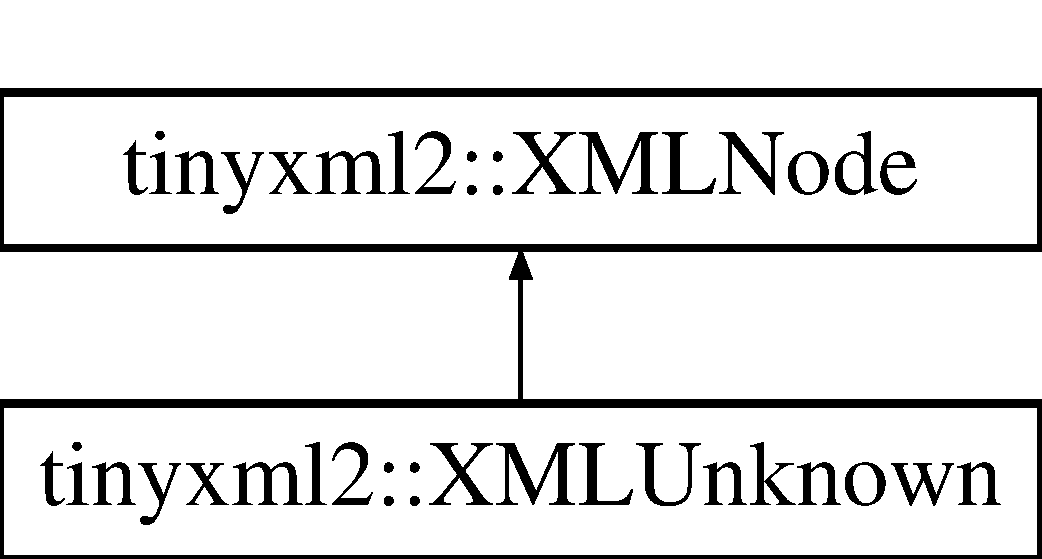
\includegraphics[height=2.000000cm]{classtinyxml2_1_1_x_m_l_unknown}
\end{center}
\end{figure}
\subsection*{Public Member Functions}
\begin{DoxyCompactItemize}
\item 
virtual \hyperlink{classtinyxml2_1_1_x_m_l_unknown}{X\-M\-L\-Unknown} $\ast$ \hyperlink{classtinyxml2_1_1_x_m_l_unknown_af4374856421921cad578c8affae872b6}{To\-Unknown} ()
\begin{DoxyCompactList}\small\item\em Safely cast to an Unknown, or null. \end{DoxyCompactList}\item 
virtual const \hyperlink{classtinyxml2_1_1_x_m_l_unknown}{X\-M\-L\-Unknown} $\ast$ \hyperlink{classtinyxml2_1_1_x_m_l_unknown_a257987e79955399e6e9f119b58d4bb30}{To\-Unknown} () const 
\item 
virtual bool \hyperlink{classtinyxml2_1_1_x_m_l_unknown_a0d341ab804a1438a474810bb5bd29dd5}{Accept} (\hyperlink{classtinyxml2_1_1_x_m_l_visitor}{X\-M\-L\-Visitor} $\ast$visitor) const 
\item 
char $\ast$ \hyperlink{classtinyxml2_1_1_x_m_l_unknown_a0e4f3509dee42a4d45a7f0002be568cc}{Parse\-Deep} (char $\ast$, \hyperlink{classtinyxml2_1_1_str_pair}{Str\-Pair} $\ast$end\-Tag)
\item 
virtual \hyperlink{classtinyxml2_1_1_x_m_l_node}{X\-M\-L\-Node} $\ast$ \hyperlink{classtinyxml2_1_1_x_m_l_unknown_aa09fc7cb0cd64d6bb9c5ae00ffc549ec}{Shallow\-Clone} (\hyperlink{classtinyxml2_1_1_x_m_l_document}{X\-M\-L\-Document} $\ast$document) const 
\item 
virtual bool \hyperlink{classtinyxml2_1_1_x_m_l_unknown_a0169df157bf69a092b404ca49621ff1a}{Shallow\-Equal} (const \hyperlink{classtinyxml2_1_1_x_m_l_node}{X\-M\-L\-Node} $\ast$compare) const 
\end{DoxyCompactItemize}
\subsection*{Protected Member Functions}
\begin{DoxyCompactItemize}
\item 
\hyperlink{classtinyxml2_1_1_x_m_l_unknown_a9391eb679598d50baba424e6f1aa367b}{X\-M\-L\-Unknown} (\hyperlink{classtinyxml2_1_1_x_m_l_document}{X\-M\-L\-Document} $\ast$doc)
\item 
virtual \hyperlink{classtinyxml2_1_1_x_m_l_unknown_a86fcd722ca173a7f385bafafa879f26e}{$\sim$\-X\-M\-L\-Unknown} ()
\item 
\hyperlink{classtinyxml2_1_1_x_m_l_unknown_aab31a93c95a7cedc9597cea7caffa73f}{X\-M\-L\-Unknown} (const \hyperlink{classtinyxml2_1_1_x_m_l_unknown}{X\-M\-L\-Unknown} \&)
\item 
\hyperlink{classtinyxml2_1_1_x_m_l_unknown}{X\-M\-L\-Unknown} \& \hyperlink{classtinyxml2_1_1_x_m_l_unknown_a6137d5611db42c35de3d869f66555e5b}{operator=} (const \hyperlink{classtinyxml2_1_1_x_m_l_unknown}{X\-M\-L\-Unknown} \&)
\end{DoxyCompactItemize}
\subsection*{Friends}
\begin{DoxyCompactItemize}
\item 
class \hyperlink{classtinyxml2_1_1_x_m_l_unknown_a4eee3bda60c60a30e4e8cd4ea91c4c6e}{X\-M\-L\-Document}
\end{DoxyCompactItemize}
\subsection*{Additional Inherited Members}


\subsection{Detailed Description}
Any tag that Tiny\-X\-M\-L-\/2 doesn't recognize is saved as an unknown. It is a tag of text, but should not be modified. It will be written back to the X\-M\-L, unchanged, when the file is saved.

D\-T\-D tags get thrown into X\-M\-L\-Unknowns. 

Definition at line 948 of file tinyxml2.\-hpp.



\subsection{Constructor \& Destructor Documentation}
\hypertarget{classtinyxml2_1_1_x_m_l_unknown_a9391eb679598d50baba424e6f1aa367b}{\index{tinyxml2\-::\-X\-M\-L\-Unknown@{tinyxml2\-::\-X\-M\-L\-Unknown}!X\-M\-L\-Unknown@{X\-M\-L\-Unknown}}
\index{X\-M\-L\-Unknown@{X\-M\-L\-Unknown}!tinyxml2::XMLUnknown@{tinyxml2\-::\-X\-M\-L\-Unknown}}
\subsubsection[{X\-M\-L\-Unknown}]{\setlength{\rightskip}{0pt plus 5cm}tinyxml2\-::\-X\-M\-L\-Unknown\-::\-X\-M\-L\-Unknown (
\begin{DoxyParamCaption}
\item[{{\bf X\-M\-L\-Document} $\ast$}]{doc}
\end{DoxyParamCaption}
)\hspace{0.3cm}{\ttfamily [protected]}}}\label{classtinyxml2_1_1_x_m_l_unknown_a9391eb679598d50baba424e6f1aa367b}


Definition at line 998 of file tinyxml2.\-cpp.

\hypertarget{classtinyxml2_1_1_x_m_l_unknown_a86fcd722ca173a7f385bafafa879f26e}{\index{tinyxml2\-::\-X\-M\-L\-Unknown@{tinyxml2\-::\-X\-M\-L\-Unknown}!$\sim$\-X\-M\-L\-Unknown@{$\sim$\-X\-M\-L\-Unknown}}
\index{$\sim$\-X\-M\-L\-Unknown@{$\sim$\-X\-M\-L\-Unknown}!tinyxml2::XMLUnknown@{tinyxml2\-::\-X\-M\-L\-Unknown}}
\subsubsection[{$\sim$\-X\-M\-L\-Unknown}]{\setlength{\rightskip}{0pt plus 5cm}tinyxml2\-::\-X\-M\-L\-Unknown\-::$\sim$\-X\-M\-L\-Unknown (
\begin{DoxyParamCaption}
{}
\end{DoxyParamCaption}
)\hspace{0.3cm}{\ttfamily [protected]}, {\ttfamily [virtual]}}}\label{classtinyxml2_1_1_x_m_l_unknown_a86fcd722ca173a7f385bafafa879f26e}


Definition at line 1003 of file tinyxml2.\-cpp.

\hypertarget{classtinyxml2_1_1_x_m_l_unknown_aab31a93c95a7cedc9597cea7caffa73f}{\index{tinyxml2\-::\-X\-M\-L\-Unknown@{tinyxml2\-::\-X\-M\-L\-Unknown}!X\-M\-L\-Unknown@{X\-M\-L\-Unknown}}
\index{X\-M\-L\-Unknown@{X\-M\-L\-Unknown}!tinyxml2::XMLUnknown@{tinyxml2\-::\-X\-M\-L\-Unknown}}
\subsubsection[{X\-M\-L\-Unknown}]{\setlength{\rightskip}{0pt plus 5cm}tinyxml2\-::\-X\-M\-L\-Unknown\-::\-X\-M\-L\-Unknown (
\begin{DoxyParamCaption}
\item[{const {\bf X\-M\-L\-Unknown} \&}]{}
\end{DoxyParamCaption}
)\hspace{0.3cm}{\ttfamily [protected]}}}\label{classtinyxml2_1_1_x_m_l_unknown_aab31a93c95a7cedc9597cea7caffa73f}


\subsection{Member Function Documentation}
\hypertarget{classtinyxml2_1_1_x_m_l_unknown_a0d341ab804a1438a474810bb5bd29dd5}{\index{tinyxml2\-::\-X\-M\-L\-Unknown@{tinyxml2\-::\-X\-M\-L\-Unknown}!Accept@{Accept}}
\index{Accept@{Accept}!tinyxml2::XMLUnknown@{tinyxml2\-::\-X\-M\-L\-Unknown}}
\subsubsection[{Accept}]{\setlength{\rightskip}{0pt plus 5cm}bool tinyxml2\-::\-X\-M\-L\-Unknown\-::\-Accept (
\begin{DoxyParamCaption}
\item[{{\bf X\-M\-L\-Visitor} $\ast$}]{visitor}
\end{DoxyParamCaption}
) const\hspace{0.3cm}{\ttfamily [virtual]}}}\label{classtinyxml2_1_1_x_m_l_unknown_a0d341ab804a1438a474810bb5bd29dd5}
Accept a hierarchical visit of the nodes in the Tiny\-X\-M\-L-\/2 D\-O\-M. Every node in the X\-M\-L tree will be conditionally visited and the host will be called back via the \hyperlink{classtinyxml2_1_1_x_m_l_visitor}{X\-M\-L\-Visitor} interface.

This is essentially a S\-A\-X interface for Tiny\-X\-M\-L-\/2. (Note however it doesn't re-\/parse the X\-M\-L for the callbacks, so the performance of Tiny\-X\-M\-L-\/2 is unchanged by using this interface versus any other.)

The interface has been based on ideas from\-:
\begin{DoxyItemize}
\item \href{http://www.saxproject.org/}{\tt http\-://www.\-saxproject.\-org/}
\item \href{http://c2.com/cgi/wiki?HierarchicalVisitorPattern}{\tt http\-://c2.\-com/cgi/wiki?\-Hierarchical\-Visitor\-Pattern}
\end{DoxyItemize}

Which are both good references for \char`\"{}visiting\char`\"{}.

An example of using \hyperlink{classtinyxml2_1_1_x_m_l_unknown_a0d341ab804a1438a474810bb5bd29dd5}{Accept()}\-: \begin{DoxyVerb}XMLPrinter printer;
tinyxmlDoc.Accept( &printer );
const char* xmlcstr = printer.CStr();
\end{DoxyVerb}
 

Implements \hyperlink{classtinyxml2_1_1_x_m_l_node_a81e66df0a44c67a7af17f3b77a152785}{tinyxml2\-::\-X\-M\-L\-Node}.



Definition at line 1037 of file tinyxml2.\-cpp.

\hypertarget{classtinyxml2_1_1_x_m_l_unknown_a6137d5611db42c35de3d869f66555e5b}{\index{tinyxml2\-::\-X\-M\-L\-Unknown@{tinyxml2\-::\-X\-M\-L\-Unknown}!operator=@{operator=}}
\index{operator=@{operator=}!tinyxml2::XMLUnknown@{tinyxml2\-::\-X\-M\-L\-Unknown}}
\subsubsection[{operator=}]{\setlength{\rightskip}{0pt plus 5cm}{\bf X\-M\-L\-Unknown}\& tinyxml2\-::\-X\-M\-L\-Unknown\-::operator= (
\begin{DoxyParamCaption}
\item[{const {\bf X\-M\-L\-Unknown} \&}]{}
\end{DoxyParamCaption}
)\hspace{0.3cm}{\ttfamily [protected]}}}\label{classtinyxml2_1_1_x_m_l_unknown_a6137d5611db42c35de3d869f66555e5b}
\hypertarget{classtinyxml2_1_1_x_m_l_unknown_a0e4f3509dee42a4d45a7f0002be568cc}{\index{tinyxml2\-::\-X\-M\-L\-Unknown@{tinyxml2\-::\-X\-M\-L\-Unknown}!Parse\-Deep@{Parse\-Deep}}
\index{Parse\-Deep@{Parse\-Deep}!tinyxml2::XMLUnknown@{tinyxml2\-::\-X\-M\-L\-Unknown}}
\subsubsection[{Parse\-Deep}]{\setlength{\rightskip}{0pt plus 5cm}char $\ast$ tinyxml2\-::\-X\-M\-L\-Unknown\-::\-Parse\-Deep (
\begin{DoxyParamCaption}
\item[{char $\ast$}]{p, }
\item[{{\bf Str\-Pair} $\ast$}]{end\-Tag}
\end{DoxyParamCaption}
)\hspace{0.3cm}{\ttfamily [virtual]}}}\label{classtinyxml2_1_1_x_m_l_unknown_a0e4f3509dee42a4d45a7f0002be568cc}


Reimplemented from \hyperlink{classtinyxml2_1_1_x_m_l_node_a7610d0f603e8b603d2078521811a23c1}{tinyxml2\-::\-X\-M\-L\-Node}.



Definition at line 1008 of file tinyxml2.\-cpp.

\hypertarget{classtinyxml2_1_1_x_m_l_unknown_aa09fc7cb0cd64d6bb9c5ae00ffc549ec}{\index{tinyxml2\-::\-X\-M\-L\-Unknown@{tinyxml2\-::\-X\-M\-L\-Unknown}!Shallow\-Clone@{Shallow\-Clone}}
\index{Shallow\-Clone@{Shallow\-Clone}!tinyxml2::XMLUnknown@{tinyxml2\-::\-X\-M\-L\-Unknown}}
\subsubsection[{Shallow\-Clone}]{\setlength{\rightskip}{0pt plus 5cm}{\bf X\-M\-L\-Node} $\ast$ tinyxml2\-::\-X\-M\-L\-Unknown\-::\-Shallow\-Clone (
\begin{DoxyParamCaption}
\item[{{\bf X\-M\-L\-Document} $\ast$}]{document}
\end{DoxyParamCaption}
) const\hspace{0.3cm}{\ttfamily [virtual]}}}\label{classtinyxml2_1_1_x_m_l_unknown_aa09fc7cb0cd64d6bb9c5ae00ffc549ec}
Make a copy of this node, but not its children. You may pass in a Document pointer that will be the owner of the new Node. If the 'document' is null, then the node returned will be allocated from the current Document. (this-\/$>$\hyperlink{classtinyxml2_1_1_x_m_l_node_af343d1ef0b45c0020e62d784d7e67a68}{Get\-Document()})

Note\-: if called on a \hyperlink{classtinyxml2_1_1_x_m_l_document}{X\-M\-L\-Document}, this will return null. 

Implements \hyperlink{classtinyxml2_1_1_x_m_l_node_a8402cbd3129d20e9e6024bbcc0531283}{tinyxml2\-::\-X\-M\-L\-Node}.



Definition at line 1021 of file tinyxml2.\-cpp.

\hypertarget{classtinyxml2_1_1_x_m_l_unknown_a0169df157bf69a092b404ca49621ff1a}{\index{tinyxml2\-::\-X\-M\-L\-Unknown@{tinyxml2\-::\-X\-M\-L\-Unknown}!Shallow\-Equal@{Shallow\-Equal}}
\index{Shallow\-Equal@{Shallow\-Equal}!tinyxml2::XMLUnknown@{tinyxml2\-::\-X\-M\-L\-Unknown}}
\subsubsection[{Shallow\-Equal}]{\setlength{\rightskip}{0pt plus 5cm}bool tinyxml2\-::\-X\-M\-L\-Unknown\-::\-Shallow\-Equal (
\begin{DoxyParamCaption}
\item[{const {\bf X\-M\-L\-Node} $\ast$}]{compare}
\end{DoxyParamCaption}
) const\hspace{0.3cm}{\ttfamily [virtual]}}}\label{classtinyxml2_1_1_x_m_l_unknown_a0169df157bf69a092b404ca49621ff1a}
Test if 2 nodes are the same, but don't test children. The 2 nodes do not need to be in the same Document.

Note\-: if called on a \hyperlink{classtinyxml2_1_1_x_m_l_document}{X\-M\-L\-Document}, this will return false. 

Implements \hyperlink{classtinyxml2_1_1_x_m_l_node_a7ce18b751c3ea09eac292dca264f9226}{tinyxml2\-::\-X\-M\-L\-Node}.



Definition at line 1031 of file tinyxml2.\-cpp.

\hypertarget{classtinyxml2_1_1_x_m_l_unknown_af4374856421921cad578c8affae872b6}{\index{tinyxml2\-::\-X\-M\-L\-Unknown@{tinyxml2\-::\-X\-M\-L\-Unknown}!To\-Unknown@{To\-Unknown}}
\index{To\-Unknown@{To\-Unknown}!tinyxml2::XMLUnknown@{tinyxml2\-::\-X\-M\-L\-Unknown}}
\subsubsection[{To\-Unknown}]{\setlength{\rightskip}{0pt plus 5cm}virtual {\bf X\-M\-L\-Unknown}$\ast$ tinyxml2\-::\-X\-M\-L\-Unknown\-::\-To\-Unknown (
\begin{DoxyParamCaption}
{}
\end{DoxyParamCaption}
)\hspace{0.3cm}{\ttfamily [inline]}, {\ttfamily [virtual]}}}\label{classtinyxml2_1_1_x_m_l_unknown_af4374856421921cad578c8affae872b6}


Safely cast to an Unknown, or null. 



Reimplemented from \hyperlink{classtinyxml2_1_1_x_m_l_node_a8675a74aa0ada6eccab0c77ef3e5b9bd}{tinyxml2\-::\-X\-M\-L\-Node}.



Definition at line 952 of file tinyxml2.\-hpp.

\hypertarget{classtinyxml2_1_1_x_m_l_unknown_a257987e79955399e6e9f119b58d4bb30}{\index{tinyxml2\-::\-X\-M\-L\-Unknown@{tinyxml2\-::\-X\-M\-L\-Unknown}!To\-Unknown@{To\-Unknown}}
\index{To\-Unknown@{To\-Unknown}!tinyxml2::XMLUnknown@{tinyxml2\-::\-X\-M\-L\-Unknown}}
\subsubsection[{To\-Unknown}]{\setlength{\rightskip}{0pt plus 5cm}virtual const {\bf X\-M\-L\-Unknown}$\ast$ tinyxml2\-::\-X\-M\-L\-Unknown\-::\-To\-Unknown (
\begin{DoxyParamCaption}
{}
\end{DoxyParamCaption}
) const\hspace{0.3cm}{\ttfamily [inline]}, {\ttfamily [virtual]}}}\label{classtinyxml2_1_1_x_m_l_unknown_a257987e79955399e6e9f119b58d4bb30}


Reimplemented from \hyperlink{classtinyxml2_1_1_x_m_l_node_a71f5ae90296dbe67979f83fe97073efa}{tinyxml2\-::\-X\-M\-L\-Node}.



Definition at line 955 of file tinyxml2.\-hpp.



\subsection{Friends And Related Function Documentation}
\hypertarget{classtinyxml2_1_1_x_m_l_unknown_a4eee3bda60c60a30e4e8cd4ea91c4c6e}{\index{tinyxml2\-::\-X\-M\-L\-Unknown@{tinyxml2\-::\-X\-M\-L\-Unknown}!X\-M\-L\-Document@{X\-M\-L\-Document}}
\index{X\-M\-L\-Document@{X\-M\-L\-Document}!tinyxml2::XMLUnknown@{tinyxml2\-::\-X\-M\-L\-Unknown}}
\subsubsection[{X\-M\-L\-Document}]{\setlength{\rightskip}{0pt plus 5cm}friend class {\bf X\-M\-L\-Document}\hspace{0.3cm}{\ttfamily [friend]}}}\label{classtinyxml2_1_1_x_m_l_unknown_a4eee3bda60c60a30e4e8cd4ea91c4c6e}


Definition at line 950 of file tinyxml2.\-hpp.



The documentation for this class was generated from the following files\-:\begin{DoxyCompactItemize}
\item 
/home/lee/\-Projects/\-Sudden\-Awakening/\-Source/\hyperlink{tinyxml2_8hpp}{tinyxml2.\-hpp}\item 
/home/lee/\-Projects/\-Sudden\-Awakening/\-Source/\hyperlink{tinyxml2_8cpp}{tinyxml2.\-cpp}\end{DoxyCompactItemize}

\hypertarget{classtinyxml2_1_1_x_m_l_util}{\section{tinyxml2\-:\-:X\-M\-L\-Util Class Reference}
\label{classtinyxml2_1_1_x_m_l_util}\index{tinyxml2\-::\-X\-M\-L\-Util@{tinyxml2\-::\-X\-M\-L\-Util}}
}


{\ttfamily \#include $<$tinyxml2.\-hpp$>$}

\subsection*{Static Public Member Functions}
\begin{DoxyCompactItemize}
\item 
static const char $\ast$ \hyperlink{classtinyxml2_1_1_x_m_l_util_a9333d20f2a34325b5115ca45849c4b2a}{Skip\-White\-Space} (const char $\ast$p)
\item 
static char $\ast$ \hyperlink{classtinyxml2_1_1_x_m_l_util_aa48025be8843ec5a79b65579d31bd8fc}{Skip\-White\-Space} (char $\ast$p)
\item 
static bool \hyperlink{classtinyxml2_1_1_x_m_l_util_a357ec3af8fc433d19023a815f45e8e33}{Is\-White\-Space} (char p)
\item 
static bool \hyperlink{classtinyxml2_1_1_x_m_l_util_abe106a69ac4d942a4381a4d9dfd0e0bd}{Is\-Name\-Start\-Char} (unsigned char ch)
\item 
static bool \hyperlink{classtinyxml2_1_1_x_m_l_util_a04b17341538fa11752f24b4301d19485}{Is\-Name\-Char} (unsigned char ch)
\item 
static bool \hyperlink{classtinyxml2_1_1_x_m_l_util_acfcd287cacfd2533e1bc9ea4dfb56602}{String\-Equal} (const char $\ast$p, const char $\ast$q, int n\-Char=I\-N\-T\-\_\-\-M\-A\-X)
\item 
static int \hyperlink{classtinyxml2_1_1_x_m_l_util_a24ba87b1d22528167a3d16c4f52096bf}{Is\-U\-T\-F8\-Continuation} (const char p)
\item 
static const char $\ast$ \hyperlink{classtinyxml2_1_1_x_m_l_util_ae9bcb2bc3cd6475fdc644c8c17790555}{Read\-B\-O\-M} (const char $\ast$p, bool $\ast$has\-B\-O\-M)
\item 
static const char $\ast$ \hyperlink{classtinyxml2_1_1_x_m_l_util_a5a96e5144a8d693dc4bcd783d9964648}{Get\-Character\-Ref} (const char $\ast$p, char $\ast$value, int $\ast$length)
\item 
static void \hyperlink{classtinyxml2_1_1_x_m_l_util_a31c00d5c5dfb38382de1dfcaf4be3595}{Convert\-U\-T\-F32\-To\-U\-T\-F8} (unsigned long input, char $\ast$output, int $\ast$length)
\item 
static void \hyperlink{classtinyxml2_1_1_x_m_l_util_a3cd6c703d49b9d51bdf0f4ff6aa021c7}{To\-Str} (int v, char $\ast$buffer, int buffer\-Size)
\item 
static void \hyperlink{classtinyxml2_1_1_x_m_l_util_ac00c2e52c1c36dab3ff41d86a9bf60f9}{To\-Str} (unsigned v, char $\ast$buffer, int buffer\-Size)
\item 
static void \hyperlink{classtinyxml2_1_1_x_m_l_util_adba0718527ae9e80f663a71ea325cb11}{To\-Str} (bool v, char $\ast$buffer, int buffer\-Size)
\item 
static void \hyperlink{classtinyxml2_1_1_x_m_l_util_a8957ad44fee5fa02ba52d73aad4d0a31}{To\-Str} (float v, char $\ast$buffer, int buffer\-Size)
\item 
static void \hyperlink{classtinyxml2_1_1_x_m_l_util_a1cd141e50980fcddd6bf9af5de4b1db7}{To\-Str} (double v, char $\ast$buffer, int buffer\-Size)
\item 
static bool \hyperlink{classtinyxml2_1_1_x_m_l_util_ad4df4023d11ee3fca9689c49b9707323}{To\-Int} (const char $\ast$str, int $\ast$value)
\item 
static bool \hyperlink{classtinyxml2_1_1_x_m_l_util_a210c8637d5eb4ce3d4625294af0efc2f}{To\-Unsigned} (const char $\ast$str, unsigned $\ast$value)
\item 
static bool \hyperlink{classtinyxml2_1_1_x_m_l_util_ae5b03e0a1ca5d42052a7ac540f7aa12a}{To\-Bool} (const char $\ast$str, bool $\ast$value)
\item 
static bool \hyperlink{classtinyxml2_1_1_x_m_l_util_a399e71edb5f29d61ea81d91ee0332bb9}{To\-Float} (const char $\ast$str, float $\ast$value)
\item 
static bool \hyperlink{classtinyxml2_1_1_x_m_l_util_ad8f75ac140fb19c1c6e164a957c4cd53}{To\-Double} (const char $\ast$str, double $\ast$value)
\end{DoxyCompactItemize}


\subsection{Detailed Description}


Definition at line 472 of file tinyxml2.\-hpp.



\subsection{Member Function Documentation}
\hypertarget{classtinyxml2_1_1_x_m_l_util_a31c00d5c5dfb38382de1dfcaf4be3595}{\index{tinyxml2\-::\-X\-M\-L\-Util@{tinyxml2\-::\-X\-M\-L\-Util}!Convert\-U\-T\-F32\-To\-U\-T\-F8@{Convert\-U\-T\-F32\-To\-U\-T\-F8}}
\index{Convert\-U\-T\-F32\-To\-U\-T\-F8@{Convert\-U\-T\-F32\-To\-U\-T\-F8}!tinyxml2::XMLUtil@{tinyxml2\-::\-X\-M\-L\-Util}}
\subsubsection[{Convert\-U\-T\-F32\-To\-U\-T\-F8}]{\setlength{\rightskip}{0pt plus 5cm}void tinyxml2\-::\-X\-M\-L\-Util\-::\-Convert\-U\-T\-F32\-To\-U\-T\-F8 (
\begin{DoxyParamCaption}
\item[{unsigned long}]{input, }
\item[{char $\ast$}]{output, }
\item[{int $\ast$}]{length}
\end{DoxyParamCaption}
)\hspace{0.3cm}{\ttfamily [static]}}}\label{classtinyxml2_1_1_x_m_l_util_a31c00d5c5dfb38382de1dfcaf4be3595}


Definition at line 282 of file tinyxml2.\-cpp.

\hypertarget{classtinyxml2_1_1_x_m_l_util_a5a96e5144a8d693dc4bcd783d9964648}{\index{tinyxml2\-::\-X\-M\-L\-Util@{tinyxml2\-::\-X\-M\-L\-Util}!Get\-Character\-Ref@{Get\-Character\-Ref}}
\index{Get\-Character\-Ref@{Get\-Character\-Ref}!tinyxml2::XMLUtil@{tinyxml2\-::\-X\-M\-L\-Util}}
\subsubsection[{Get\-Character\-Ref}]{\setlength{\rightskip}{0pt plus 5cm}const char $\ast$ tinyxml2\-::\-X\-M\-L\-Util\-::\-Get\-Character\-Ref (
\begin{DoxyParamCaption}
\item[{const char $\ast$}]{p, }
\item[{char $\ast$}]{value, }
\item[{int $\ast$}]{length}
\end{DoxyParamCaption}
)\hspace{0.3cm}{\ttfamily [static]}}}\label{classtinyxml2_1_1_x_m_l_util_a5a96e5144a8d693dc4bcd783d9964648}


Definition at line 330 of file tinyxml2.\-cpp.

\hypertarget{classtinyxml2_1_1_x_m_l_util_a04b17341538fa11752f24b4301d19485}{\index{tinyxml2\-::\-X\-M\-L\-Util@{tinyxml2\-::\-X\-M\-L\-Util}!Is\-Name\-Char@{Is\-Name\-Char}}
\index{Is\-Name\-Char@{Is\-Name\-Char}!tinyxml2::XMLUtil@{tinyxml2\-::\-X\-M\-L\-Util}}
\subsubsection[{Is\-Name\-Char}]{\setlength{\rightskip}{0pt plus 5cm}static bool tinyxml2\-::\-X\-M\-L\-Util\-::\-Is\-Name\-Char (
\begin{DoxyParamCaption}
\item[{unsigned char}]{ch}
\end{DoxyParamCaption}
)\hspace{0.3cm}{\ttfamily [inline]}, {\ttfamily [static]}}}\label{classtinyxml2_1_1_x_m_l_util_a04b17341538fa11752f24b4301d19485}


Definition at line 499 of file tinyxml2.\-hpp.

\hypertarget{classtinyxml2_1_1_x_m_l_util_abe106a69ac4d942a4381a4d9dfd0e0bd}{\index{tinyxml2\-::\-X\-M\-L\-Util@{tinyxml2\-::\-X\-M\-L\-Util}!Is\-Name\-Start\-Char@{Is\-Name\-Start\-Char}}
\index{Is\-Name\-Start\-Char@{Is\-Name\-Start\-Char}!tinyxml2::XMLUtil@{tinyxml2\-::\-X\-M\-L\-Util}}
\subsubsection[{Is\-Name\-Start\-Char}]{\setlength{\rightskip}{0pt plus 5cm}static bool tinyxml2\-::\-X\-M\-L\-Util\-::\-Is\-Name\-Start\-Char (
\begin{DoxyParamCaption}
\item[{unsigned char}]{ch}
\end{DoxyParamCaption}
)\hspace{0.3cm}{\ttfamily [inline]}, {\ttfamily [static]}}}\label{classtinyxml2_1_1_x_m_l_util_abe106a69ac4d942a4381a4d9dfd0e0bd}


Definition at line 493 of file tinyxml2.\-hpp.

\hypertarget{classtinyxml2_1_1_x_m_l_util_a24ba87b1d22528167a3d16c4f52096bf}{\index{tinyxml2\-::\-X\-M\-L\-Util@{tinyxml2\-::\-X\-M\-L\-Util}!Is\-U\-T\-F8\-Continuation@{Is\-U\-T\-F8\-Continuation}}
\index{Is\-U\-T\-F8\-Continuation@{Is\-U\-T\-F8\-Continuation}!tinyxml2::XMLUtil@{tinyxml2\-::\-X\-M\-L\-Util}}
\subsubsection[{Is\-U\-T\-F8\-Continuation}]{\setlength{\rightskip}{0pt plus 5cm}static int tinyxml2\-::\-X\-M\-L\-Util\-::\-Is\-U\-T\-F8\-Continuation (
\begin{DoxyParamCaption}
\item[{const char}]{p}
\end{DoxyParamCaption}
)\hspace{0.3cm}{\ttfamily [inline]}, {\ttfamily [static]}}}\label{classtinyxml2_1_1_x_m_l_util_a24ba87b1d22528167a3d16c4f52096bf}


Definition at line 522 of file tinyxml2.\-hpp.

\hypertarget{classtinyxml2_1_1_x_m_l_util_a357ec3af8fc433d19023a815f45e8e33}{\index{tinyxml2\-::\-X\-M\-L\-Util@{tinyxml2\-::\-X\-M\-L\-Util}!Is\-White\-Space@{Is\-White\-Space}}
\index{Is\-White\-Space@{Is\-White\-Space}!tinyxml2::XMLUtil@{tinyxml2\-::\-X\-M\-L\-Util}}
\subsubsection[{Is\-White\-Space}]{\setlength{\rightskip}{0pt plus 5cm}static bool tinyxml2\-::\-X\-M\-L\-Util\-::\-Is\-White\-Space (
\begin{DoxyParamCaption}
\item[{char}]{p}
\end{DoxyParamCaption}
)\hspace{0.3cm}{\ttfamily [inline]}, {\ttfamily [static]}}}\label{classtinyxml2_1_1_x_m_l_util_a357ec3af8fc433d19023a815f45e8e33}


Definition at line 489 of file tinyxml2.\-hpp.

\hypertarget{classtinyxml2_1_1_x_m_l_util_ae9bcb2bc3cd6475fdc644c8c17790555}{\index{tinyxml2\-::\-X\-M\-L\-Util@{tinyxml2\-::\-X\-M\-L\-Util}!Read\-B\-O\-M@{Read\-B\-O\-M}}
\index{Read\-B\-O\-M@{Read\-B\-O\-M}!tinyxml2::XMLUtil@{tinyxml2\-::\-X\-M\-L\-Util}}
\subsubsection[{Read\-B\-O\-M}]{\setlength{\rightskip}{0pt plus 5cm}const char $\ast$ tinyxml2\-::\-X\-M\-L\-Util\-::\-Read\-B\-O\-M (
\begin{DoxyParamCaption}
\item[{const char $\ast$}]{p, }
\item[{bool $\ast$}]{has\-B\-O\-M}
\end{DoxyParamCaption}
)\hspace{0.3cm}{\ttfamily [static]}}}\label{classtinyxml2_1_1_x_m_l_util_ae9bcb2bc3cd6475fdc644c8c17790555}


Definition at line 267 of file tinyxml2.\-cpp.

\hypertarget{classtinyxml2_1_1_x_m_l_util_a9333d20f2a34325b5115ca45849c4b2a}{\index{tinyxml2\-::\-X\-M\-L\-Util@{tinyxml2\-::\-X\-M\-L\-Util}!Skip\-White\-Space@{Skip\-White\-Space}}
\index{Skip\-White\-Space@{Skip\-White\-Space}!tinyxml2::XMLUtil@{tinyxml2\-::\-X\-M\-L\-Util}}
\subsubsection[{Skip\-White\-Space}]{\setlength{\rightskip}{0pt plus 5cm}static const char$\ast$ tinyxml2\-::\-X\-M\-L\-Util\-::\-Skip\-White\-Space (
\begin{DoxyParamCaption}
\item[{const char $\ast$}]{p}
\end{DoxyParamCaption}
)\hspace{0.3cm}{\ttfamily [inline]}, {\ttfamily [static]}}}\label{classtinyxml2_1_1_x_m_l_util_a9333d20f2a34325b5115ca45849c4b2a}


Definition at line 477 of file tinyxml2.\-hpp.

\hypertarget{classtinyxml2_1_1_x_m_l_util_aa48025be8843ec5a79b65579d31bd8fc}{\index{tinyxml2\-::\-X\-M\-L\-Util@{tinyxml2\-::\-X\-M\-L\-Util}!Skip\-White\-Space@{Skip\-White\-Space}}
\index{Skip\-White\-Space@{Skip\-White\-Space}!tinyxml2::XMLUtil@{tinyxml2\-::\-X\-M\-L\-Util}}
\subsubsection[{Skip\-White\-Space}]{\setlength{\rightskip}{0pt plus 5cm}static char$\ast$ tinyxml2\-::\-X\-M\-L\-Util\-::\-Skip\-White\-Space (
\begin{DoxyParamCaption}
\item[{char $\ast$}]{p}
\end{DoxyParamCaption}
)\hspace{0.3cm}{\ttfamily [inline]}, {\ttfamily [static]}}}\label{classtinyxml2_1_1_x_m_l_util_aa48025be8843ec5a79b65579d31bd8fc}


Definition at line 483 of file tinyxml2.\-hpp.

\hypertarget{classtinyxml2_1_1_x_m_l_util_acfcd287cacfd2533e1bc9ea4dfb56602}{\index{tinyxml2\-::\-X\-M\-L\-Util@{tinyxml2\-::\-X\-M\-L\-Util}!String\-Equal@{String\-Equal}}
\index{String\-Equal@{String\-Equal}!tinyxml2::XMLUtil@{tinyxml2\-::\-X\-M\-L\-Util}}
\subsubsection[{String\-Equal}]{\setlength{\rightskip}{0pt plus 5cm}static bool tinyxml2\-::\-X\-M\-L\-Util\-::\-String\-Equal (
\begin{DoxyParamCaption}
\item[{const char $\ast$}]{p, }
\item[{const char $\ast$}]{q, }
\item[{int}]{n\-Char = {\ttfamily INT\-\_\-MAX}}
\end{DoxyParamCaption}
)\hspace{0.3cm}{\ttfamily [inline]}, {\ttfamily [static]}}}\label{classtinyxml2_1_1_x_m_l_util_acfcd287cacfd2533e1bc9ea4dfb56602}


Definition at line 506 of file tinyxml2.\-hpp.

\hypertarget{classtinyxml2_1_1_x_m_l_util_ae5b03e0a1ca5d42052a7ac540f7aa12a}{\index{tinyxml2\-::\-X\-M\-L\-Util@{tinyxml2\-::\-X\-M\-L\-Util}!To\-Bool@{To\-Bool}}
\index{To\-Bool@{To\-Bool}!tinyxml2::XMLUtil@{tinyxml2\-::\-X\-M\-L\-Util}}
\subsubsection[{To\-Bool}]{\setlength{\rightskip}{0pt plus 5cm}bool tinyxml2\-::\-X\-M\-L\-Util\-::\-To\-Bool (
\begin{DoxyParamCaption}
\item[{const char $\ast$}]{str, }
\item[{bool $\ast$}]{value}
\end{DoxyParamCaption}
)\hspace{0.3cm}{\ttfamily [static]}}}\label{classtinyxml2_1_1_x_m_l_util_ae5b03e0a1ca5d42052a7ac540f7aa12a}


Definition at line 454 of file tinyxml2.\-cpp.

\hypertarget{classtinyxml2_1_1_x_m_l_util_ad8f75ac140fb19c1c6e164a957c4cd53}{\index{tinyxml2\-::\-X\-M\-L\-Util@{tinyxml2\-::\-X\-M\-L\-Util}!To\-Double@{To\-Double}}
\index{To\-Double@{To\-Double}!tinyxml2::XMLUtil@{tinyxml2\-::\-X\-M\-L\-Util}}
\subsubsection[{To\-Double}]{\setlength{\rightskip}{0pt plus 5cm}bool tinyxml2\-::\-X\-M\-L\-Util\-::\-To\-Double (
\begin{DoxyParamCaption}
\item[{const char $\ast$}]{str, }
\item[{double $\ast$}]{value}
\end{DoxyParamCaption}
)\hspace{0.3cm}{\ttfamily [static]}}}\label{classtinyxml2_1_1_x_m_l_util_ad8f75ac140fb19c1c6e164a957c4cd53}


Definition at line 481 of file tinyxml2.\-cpp.

\hypertarget{classtinyxml2_1_1_x_m_l_util_a399e71edb5f29d61ea81d91ee0332bb9}{\index{tinyxml2\-::\-X\-M\-L\-Util@{tinyxml2\-::\-X\-M\-L\-Util}!To\-Float@{To\-Float}}
\index{To\-Float@{To\-Float}!tinyxml2::XMLUtil@{tinyxml2\-::\-X\-M\-L\-Util}}
\subsubsection[{To\-Float}]{\setlength{\rightskip}{0pt plus 5cm}bool tinyxml2\-::\-X\-M\-L\-Util\-::\-To\-Float (
\begin{DoxyParamCaption}
\item[{const char $\ast$}]{str, }
\item[{float $\ast$}]{value}
\end{DoxyParamCaption}
)\hspace{0.3cm}{\ttfamily [static]}}}\label{classtinyxml2_1_1_x_m_l_util_a399e71edb5f29d61ea81d91ee0332bb9}


Definition at line 473 of file tinyxml2.\-cpp.

\hypertarget{classtinyxml2_1_1_x_m_l_util_ad4df4023d11ee3fca9689c49b9707323}{\index{tinyxml2\-::\-X\-M\-L\-Util@{tinyxml2\-::\-X\-M\-L\-Util}!To\-Int@{To\-Int}}
\index{To\-Int@{To\-Int}!tinyxml2::XMLUtil@{tinyxml2\-::\-X\-M\-L\-Util}}
\subsubsection[{To\-Int}]{\setlength{\rightskip}{0pt plus 5cm}bool tinyxml2\-::\-X\-M\-L\-Util\-::\-To\-Int (
\begin{DoxyParamCaption}
\item[{const char $\ast$}]{str, }
\item[{int $\ast$}]{value}
\end{DoxyParamCaption}
)\hspace{0.3cm}{\ttfamily [static]}}}\label{classtinyxml2_1_1_x_m_l_util_ad4df4023d11ee3fca9689c49b9707323}


Definition at line 438 of file tinyxml2.\-cpp.

\hypertarget{classtinyxml2_1_1_x_m_l_util_a3cd6c703d49b9d51bdf0f4ff6aa021c7}{\index{tinyxml2\-::\-X\-M\-L\-Util@{tinyxml2\-::\-X\-M\-L\-Util}!To\-Str@{To\-Str}}
\index{To\-Str@{To\-Str}!tinyxml2::XMLUtil@{tinyxml2\-::\-X\-M\-L\-Util}}
\subsubsection[{To\-Str}]{\setlength{\rightskip}{0pt plus 5cm}void tinyxml2\-::\-X\-M\-L\-Util\-::\-To\-Str (
\begin{DoxyParamCaption}
\item[{int}]{v, }
\item[{char $\ast$}]{buffer, }
\item[{int}]{buffer\-Size}
\end{DoxyParamCaption}
)\hspace{0.3cm}{\ttfamily [static]}}}\label{classtinyxml2_1_1_x_m_l_util_a3cd6c703d49b9d51bdf0f4ff6aa021c7}


Definition at line 408 of file tinyxml2.\-cpp.

\hypertarget{classtinyxml2_1_1_x_m_l_util_ac00c2e52c1c36dab3ff41d86a9bf60f9}{\index{tinyxml2\-::\-X\-M\-L\-Util@{tinyxml2\-::\-X\-M\-L\-Util}!To\-Str@{To\-Str}}
\index{To\-Str@{To\-Str}!tinyxml2::XMLUtil@{tinyxml2\-::\-X\-M\-L\-Util}}
\subsubsection[{To\-Str}]{\setlength{\rightskip}{0pt plus 5cm}void tinyxml2\-::\-X\-M\-L\-Util\-::\-To\-Str (
\begin{DoxyParamCaption}
\item[{unsigned}]{v, }
\item[{char $\ast$}]{buffer, }
\item[{int}]{buffer\-Size}
\end{DoxyParamCaption}
)\hspace{0.3cm}{\ttfamily [static]}}}\label{classtinyxml2_1_1_x_m_l_util_ac00c2e52c1c36dab3ff41d86a9bf60f9}


Definition at line 414 of file tinyxml2.\-cpp.

\hypertarget{classtinyxml2_1_1_x_m_l_util_adba0718527ae9e80f663a71ea325cb11}{\index{tinyxml2\-::\-X\-M\-L\-Util@{tinyxml2\-::\-X\-M\-L\-Util}!To\-Str@{To\-Str}}
\index{To\-Str@{To\-Str}!tinyxml2::XMLUtil@{tinyxml2\-::\-X\-M\-L\-Util}}
\subsubsection[{To\-Str}]{\setlength{\rightskip}{0pt plus 5cm}void tinyxml2\-::\-X\-M\-L\-Util\-::\-To\-Str (
\begin{DoxyParamCaption}
\item[{bool}]{v, }
\item[{char $\ast$}]{buffer, }
\item[{int}]{buffer\-Size}
\end{DoxyParamCaption}
)\hspace{0.3cm}{\ttfamily [static]}}}\label{classtinyxml2_1_1_x_m_l_util_adba0718527ae9e80f663a71ea325cb11}


Definition at line 420 of file tinyxml2.\-cpp.

\hypertarget{classtinyxml2_1_1_x_m_l_util_a8957ad44fee5fa02ba52d73aad4d0a31}{\index{tinyxml2\-::\-X\-M\-L\-Util@{tinyxml2\-::\-X\-M\-L\-Util}!To\-Str@{To\-Str}}
\index{To\-Str@{To\-Str}!tinyxml2::XMLUtil@{tinyxml2\-::\-X\-M\-L\-Util}}
\subsubsection[{To\-Str}]{\setlength{\rightskip}{0pt plus 5cm}void tinyxml2\-::\-X\-M\-L\-Util\-::\-To\-Str (
\begin{DoxyParamCaption}
\item[{float}]{v, }
\item[{char $\ast$}]{buffer, }
\item[{int}]{buffer\-Size}
\end{DoxyParamCaption}
)\hspace{0.3cm}{\ttfamily [static]}}}\label{classtinyxml2_1_1_x_m_l_util_a8957ad44fee5fa02ba52d73aad4d0a31}


Definition at line 426 of file tinyxml2.\-cpp.

\hypertarget{classtinyxml2_1_1_x_m_l_util_a1cd141e50980fcddd6bf9af5de4b1db7}{\index{tinyxml2\-::\-X\-M\-L\-Util@{tinyxml2\-::\-X\-M\-L\-Util}!To\-Str@{To\-Str}}
\index{To\-Str@{To\-Str}!tinyxml2::XMLUtil@{tinyxml2\-::\-X\-M\-L\-Util}}
\subsubsection[{To\-Str}]{\setlength{\rightskip}{0pt plus 5cm}void tinyxml2\-::\-X\-M\-L\-Util\-::\-To\-Str (
\begin{DoxyParamCaption}
\item[{double}]{v, }
\item[{char $\ast$}]{buffer, }
\item[{int}]{buffer\-Size}
\end{DoxyParamCaption}
)\hspace{0.3cm}{\ttfamily [static]}}}\label{classtinyxml2_1_1_x_m_l_util_a1cd141e50980fcddd6bf9af5de4b1db7}


Definition at line 432 of file tinyxml2.\-cpp.

\hypertarget{classtinyxml2_1_1_x_m_l_util_a210c8637d5eb4ce3d4625294af0efc2f}{\index{tinyxml2\-::\-X\-M\-L\-Util@{tinyxml2\-::\-X\-M\-L\-Util}!To\-Unsigned@{To\-Unsigned}}
\index{To\-Unsigned@{To\-Unsigned}!tinyxml2::XMLUtil@{tinyxml2\-::\-X\-M\-L\-Util}}
\subsubsection[{To\-Unsigned}]{\setlength{\rightskip}{0pt plus 5cm}bool tinyxml2\-::\-X\-M\-L\-Util\-::\-To\-Unsigned (
\begin{DoxyParamCaption}
\item[{const char $\ast$}]{str, }
\item[{unsigned $\ast$}]{value}
\end{DoxyParamCaption}
)\hspace{0.3cm}{\ttfamily [static]}}}\label{classtinyxml2_1_1_x_m_l_util_a210c8637d5eb4ce3d4625294af0efc2f}


Definition at line 446 of file tinyxml2.\-cpp.



The documentation for this class was generated from the following files\-:\begin{DoxyCompactItemize}
\item 
Source/\hyperlink{tinyxml2_8hpp}{tinyxml2.\-hpp}\item 
Source/\hyperlink{tinyxml2_8cpp}{tinyxml2.\-cpp}\end{DoxyCompactItemize}

\hypertarget{classtinyxml2_1_1_x_m_l_visitor}{\section{tinyxml2\-:\-:X\-M\-L\-Visitor Class Reference}
\label{classtinyxml2_1_1_x_m_l_visitor}\index{tinyxml2\-::\-X\-M\-L\-Visitor@{tinyxml2\-::\-X\-M\-L\-Visitor}}
}


{\ttfamily \#include $<$tinyxml2.\-hpp$>$}

Inheritance diagram for tinyxml2\-:\-:X\-M\-L\-Visitor\-:\begin{figure}[H]
\begin{center}
\leavevmode
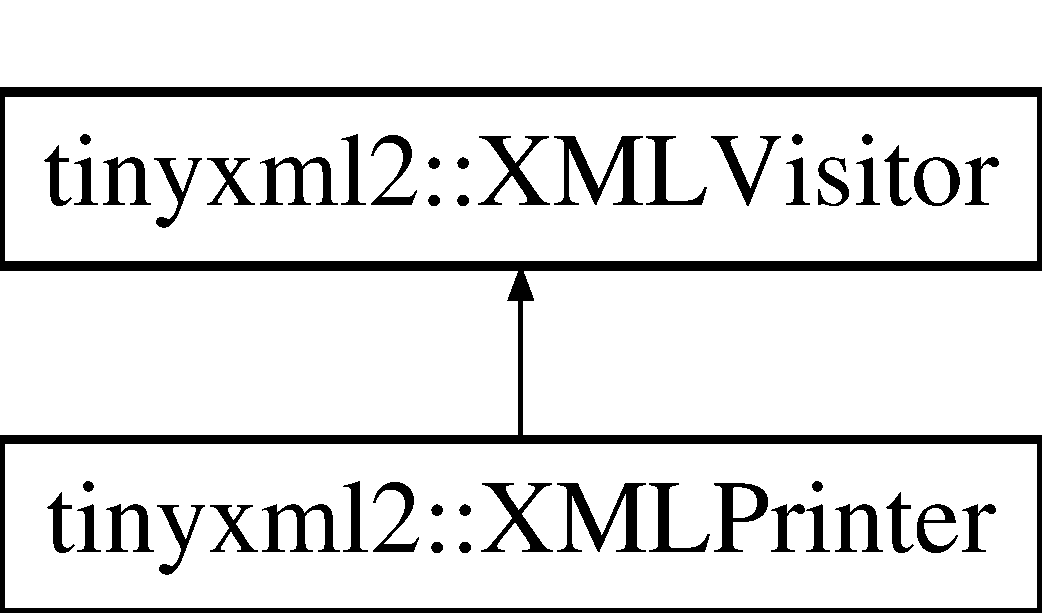
\includegraphics[height=2.000000cm]{classtinyxml2_1_1_x_m_l_visitor}
\end{center}
\end{figure}
\subsection*{Public Member Functions}
\begin{DoxyCompactItemize}
\item 
virtual \hyperlink{classtinyxml2_1_1_x_m_l_visitor_a494e72033d646c47d9c65c502ec62364}{$\sim$\-X\-M\-L\-Visitor} ()
\item 
virtual bool \hyperlink{classtinyxml2_1_1_x_m_l_visitor_acb3c22fc5f60eb9db98f533f2761f67d}{Visit\-Enter} (const \hyperlink{classtinyxml2_1_1_x_m_l_document}{X\-M\-L\-Document} \&)
\begin{DoxyCompactList}\small\item\em Visit a document. \end{DoxyCompactList}\item 
virtual bool \hyperlink{classtinyxml2_1_1_x_m_l_visitor_a170e9989cd046ba904f302d087e07086}{Visit\-Exit} (const \hyperlink{classtinyxml2_1_1_x_m_l_document}{X\-M\-L\-Document} \&)
\begin{DoxyCompactList}\small\item\em Visit a document. \end{DoxyCompactList}\item 
virtual bool \hyperlink{classtinyxml2_1_1_x_m_l_visitor_af97980a17dd4e37448b181f5ddfa92b5}{Visit\-Enter} (const \hyperlink{classtinyxml2_1_1_x_m_l_element}{X\-M\-L\-Element} \&, const \hyperlink{classtinyxml2_1_1_x_m_l_attribute}{X\-M\-L\-Attribute} $\ast$)
\begin{DoxyCompactList}\small\item\em Visit an element. \end{DoxyCompactList}\item 
virtual bool \hyperlink{classtinyxml2_1_1_x_m_l_visitor_a772f10ddc83f881956d32628faa16eb6}{Visit\-Exit} (const \hyperlink{classtinyxml2_1_1_x_m_l_element}{X\-M\-L\-Element} \&)
\begin{DoxyCompactList}\small\item\em Visit an element. \end{DoxyCompactList}\item 
virtual bool \hyperlink{classtinyxml2_1_1_x_m_l_visitor_adc75bd459fc7ba8223b50f0616767f9a}{Visit} (const \hyperlink{classtinyxml2_1_1_x_m_l_declaration}{X\-M\-L\-Declaration} \&)
\begin{DoxyCompactList}\small\item\em Visit a declaration. \end{DoxyCompactList}\item 
virtual bool \hyperlink{classtinyxml2_1_1_x_m_l_visitor_af30233565856480ea48b6fa0d6dec65b}{Visit} (const \hyperlink{classtinyxml2_1_1_x_m_l_text}{X\-M\-L\-Text} \&)
\begin{DoxyCompactList}\small\item\em Visit a text node. \end{DoxyCompactList}\item 
virtual bool \hyperlink{classtinyxml2_1_1_x_m_l_visitor_acc8147fb5a85f6c65721654e427752d7}{Visit} (const \hyperlink{classtinyxml2_1_1_x_m_l_comment}{X\-M\-L\-Comment} \&)
\begin{DoxyCompactList}\small\item\em Visit a comment node. \end{DoxyCompactList}\item 
virtual bool \hyperlink{classtinyxml2_1_1_x_m_l_visitor_a14e4748387c34bf53d24e8119bb1f292}{Visit} (const \hyperlink{classtinyxml2_1_1_x_m_l_unknown}{X\-M\-L\-Unknown} \&)
\begin{DoxyCompactList}\small\item\em Visit an unknown node. \end{DoxyCompactList}\end{DoxyCompactItemize}


\subsection{Detailed Description}
Implements the interface to the \char`\"{}\-Visitor pattern\char`\"{} (see the Accept() method.) If you call the Accept() method, it requires being passed a \hyperlink{classtinyxml2_1_1_x_m_l_visitor}{X\-M\-L\-Visitor} class to handle callbacks. For nodes that contain other nodes (Document, Element) you will get called with a Visit\-Enter/\-Visit\-Exit pair. Nodes that are always leafs are simply called with \hyperlink{classtinyxml2_1_1_x_m_l_visitor_adc75bd459fc7ba8223b50f0616767f9a}{Visit()}.

If you return 'true' from a Visit method, recursive parsing will continue. If you return false, {\bfseries no children of this node or its siblings} will be visited.

All flavors of Visit methods have a default implementation that returns 'true' (continue visiting). You need to only override methods that are interesting to you.

Generally Accept() is called on the \hyperlink{classtinyxml2_1_1_x_m_l_document}{X\-M\-L\-Document}, although all nodes support visiting.

You should never change the document from a callback.

\begin{DoxySeeAlso}{See Also}
\hyperlink{classtinyxml2_1_1_x_m_l_node_a81e66df0a44c67a7af17f3b77a152785}{X\-M\-L\-Node\-::\-Accept()} 
\end{DoxySeeAlso}


Definition at line 427 of file tinyxml2.\-hpp.



\subsection{Constructor \& Destructor Documentation}
\hypertarget{classtinyxml2_1_1_x_m_l_visitor_a494e72033d646c47d9c65c502ec62364}{\index{tinyxml2\-::\-X\-M\-L\-Visitor@{tinyxml2\-::\-X\-M\-L\-Visitor}!$\sim$\-X\-M\-L\-Visitor@{$\sim$\-X\-M\-L\-Visitor}}
\index{$\sim$\-X\-M\-L\-Visitor@{$\sim$\-X\-M\-L\-Visitor}!tinyxml2::XMLVisitor@{tinyxml2\-::\-X\-M\-L\-Visitor}}
\subsubsection[{$\sim$\-X\-M\-L\-Visitor}]{\setlength{\rightskip}{0pt plus 5cm}virtual tinyxml2\-::\-X\-M\-L\-Visitor\-::$\sim$\-X\-M\-L\-Visitor (
\begin{DoxyParamCaption}
{}
\end{DoxyParamCaption}
)\hspace{0.3cm}{\ttfamily [inline]}, {\ttfamily [virtual]}}}\label{classtinyxml2_1_1_x_m_l_visitor_a494e72033d646c47d9c65c502ec62364}


Definition at line 430 of file tinyxml2.\-hpp.



\subsection{Member Function Documentation}
\hypertarget{classtinyxml2_1_1_x_m_l_visitor_adc75bd459fc7ba8223b50f0616767f9a}{\index{tinyxml2\-::\-X\-M\-L\-Visitor@{tinyxml2\-::\-X\-M\-L\-Visitor}!Visit@{Visit}}
\index{Visit@{Visit}!tinyxml2::XMLVisitor@{tinyxml2\-::\-X\-M\-L\-Visitor}}
\subsubsection[{Visit}]{\setlength{\rightskip}{0pt plus 5cm}virtual bool tinyxml2\-::\-X\-M\-L\-Visitor\-::\-Visit (
\begin{DoxyParamCaption}
\item[{const {\bf X\-M\-L\-Declaration} \&}]{}
\end{DoxyParamCaption}
)\hspace{0.3cm}{\ttfamily [inline]}, {\ttfamily [virtual]}}}\label{classtinyxml2_1_1_x_m_l_visitor_adc75bd459fc7ba8223b50f0616767f9a}


Visit a declaration. 



Reimplemented in \hyperlink{classtinyxml2_1_1_x_m_l_printer_acfc625b2549304b9c7eb85ebd5c5eb39}{tinyxml2\-::\-X\-M\-L\-Printer}.



Definition at line 451 of file tinyxml2.\-hpp.

\hypertarget{classtinyxml2_1_1_x_m_l_visitor_af30233565856480ea48b6fa0d6dec65b}{\index{tinyxml2\-::\-X\-M\-L\-Visitor@{tinyxml2\-::\-X\-M\-L\-Visitor}!Visit@{Visit}}
\index{Visit@{Visit}!tinyxml2::XMLVisitor@{tinyxml2\-::\-X\-M\-L\-Visitor}}
\subsubsection[{Visit}]{\setlength{\rightskip}{0pt plus 5cm}virtual bool tinyxml2\-::\-X\-M\-L\-Visitor\-::\-Visit (
\begin{DoxyParamCaption}
\item[{const {\bf X\-M\-L\-Text} \&}]{}
\end{DoxyParamCaption}
)\hspace{0.3cm}{\ttfamily [inline]}, {\ttfamily [virtual]}}}\label{classtinyxml2_1_1_x_m_l_visitor_af30233565856480ea48b6fa0d6dec65b}


Visit a text node. 



Reimplemented in \hyperlink{classtinyxml2_1_1_x_m_l_printer_adc0e42b4f6fcb90a95630c79575d030b}{tinyxml2\-::\-X\-M\-L\-Printer}.



Definition at line 455 of file tinyxml2.\-hpp.

\hypertarget{classtinyxml2_1_1_x_m_l_visitor_acc8147fb5a85f6c65721654e427752d7}{\index{tinyxml2\-::\-X\-M\-L\-Visitor@{tinyxml2\-::\-X\-M\-L\-Visitor}!Visit@{Visit}}
\index{Visit@{Visit}!tinyxml2::XMLVisitor@{tinyxml2\-::\-X\-M\-L\-Visitor}}
\subsubsection[{Visit}]{\setlength{\rightskip}{0pt plus 5cm}virtual bool tinyxml2\-::\-X\-M\-L\-Visitor\-::\-Visit (
\begin{DoxyParamCaption}
\item[{const {\bf X\-M\-L\-Comment} \&}]{}
\end{DoxyParamCaption}
)\hspace{0.3cm}{\ttfamily [inline]}, {\ttfamily [virtual]}}}\label{classtinyxml2_1_1_x_m_l_visitor_acc8147fb5a85f6c65721654e427752d7}


Visit a comment node. 



Reimplemented in \hyperlink{classtinyxml2_1_1_x_m_l_printer_aa294c5c01af0ebb9114902456e4cb53c}{tinyxml2\-::\-X\-M\-L\-Printer}.



Definition at line 459 of file tinyxml2.\-hpp.

\hypertarget{classtinyxml2_1_1_x_m_l_visitor_a14e4748387c34bf53d24e8119bb1f292}{\index{tinyxml2\-::\-X\-M\-L\-Visitor@{tinyxml2\-::\-X\-M\-L\-Visitor}!Visit@{Visit}}
\index{Visit@{Visit}!tinyxml2::XMLVisitor@{tinyxml2\-::\-X\-M\-L\-Visitor}}
\subsubsection[{Visit}]{\setlength{\rightskip}{0pt plus 5cm}virtual bool tinyxml2\-::\-X\-M\-L\-Visitor\-::\-Visit (
\begin{DoxyParamCaption}
\item[{const {\bf X\-M\-L\-Unknown} \&}]{}
\end{DoxyParamCaption}
)\hspace{0.3cm}{\ttfamily [inline]}, {\ttfamily [virtual]}}}\label{classtinyxml2_1_1_x_m_l_visitor_a14e4748387c34bf53d24e8119bb1f292}


Visit an unknown node. 



Reimplemented in \hyperlink{classtinyxml2_1_1_x_m_l_printer_ab8af5455bbf9e4be2663e6642fcd7e32}{tinyxml2\-::\-X\-M\-L\-Printer}.



Definition at line 463 of file tinyxml2.\-hpp.

\hypertarget{classtinyxml2_1_1_x_m_l_visitor_acb3c22fc5f60eb9db98f533f2761f67d}{\index{tinyxml2\-::\-X\-M\-L\-Visitor@{tinyxml2\-::\-X\-M\-L\-Visitor}!Visit\-Enter@{Visit\-Enter}}
\index{Visit\-Enter@{Visit\-Enter}!tinyxml2::XMLVisitor@{tinyxml2\-::\-X\-M\-L\-Visitor}}
\subsubsection[{Visit\-Enter}]{\setlength{\rightskip}{0pt plus 5cm}virtual bool tinyxml2\-::\-X\-M\-L\-Visitor\-::\-Visit\-Enter (
\begin{DoxyParamCaption}
\item[{const {\bf X\-M\-L\-Document} \&}]{}
\end{DoxyParamCaption}
)\hspace{0.3cm}{\ttfamily [inline]}, {\ttfamily [virtual]}}}\label{classtinyxml2_1_1_x_m_l_visitor_acb3c22fc5f60eb9db98f533f2761f67d}


Visit a document. 



Reimplemented in \hyperlink{classtinyxml2_1_1_x_m_l_printer_a9aa1de11a55a07db55a90fde37d7afad}{tinyxml2\-::\-X\-M\-L\-Printer}.



Definition at line 433 of file tinyxml2.\-hpp.

\hypertarget{classtinyxml2_1_1_x_m_l_visitor_af97980a17dd4e37448b181f5ddfa92b5}{\index{tinyxml2\-::\-X\-M\-L\-Visitor@{tinyxml2\-::\-X\-M\-L\-Visitor}!Visit\-Enter@{Visit\-Enter}}
\index{Visit\-Enter@{Visit\-Enter}!tinyxml2::XMLVisitor@{tinyxml2\-::\-X\-M\-L\-Visitor}}
\subsubsection[{Visit\-Enter}]{\setlength{\rightskip}{0pt plus 5cm}virtual bool tinyxml2\-::\-X\-M\-L\-Visitor\-::\-Visit\-Enter (
\begin{DoxyParamCaption}
\item[{const {\bf X\-M\-L\-Element} \&}]{, }
\item[{const {\bf X\-M\-L\-Attribute} $\ast$}]{}
\end{DoxyParamCaption}
)\hspace{0.3cm}{\ttfamily [inline]}, {\ttfamily [virtual]}}}\label{classtinyxml2_1_1_x_m_l_visitor_af97980a17dd4e37448b181f5ddfa92b5}


Visit an element. 



Reimplemented in \hyperlink{classtinyxml2_1_1_x_m_l_printer_a169b2509d8eabb70811b2bb8cfd1f5d1}{tinyxml2\-::\-X\-M\-L\-Printer}.



Definition at line 442 of file tinyxml2.\-hpp.

\hypertarget{classtinyxml2_1_1_x_m_l_visitor_a170e9989cd046ba904f302d087e07086}{\index{tinyxml2\-::\-X\-M\-L\-Visitor@{tinyxml2\-::\-X\-M\-L\-Visitor}!Visit\-Exit@{Visit\-Exit}}
\index{Visit\-Exit@{Visit\-Exit}!tinyxml2::XMLVisitor@{tinyxml2\-::\-X\-M\-L\-Visitor}}
\subsubsection[{Visit\-Exit}]{\setlength{\rightskip}{0pt plus 5cm}virtual bool tinyxml2\-::\-X\-M\-L\-Visitor\-::\-Visit\-Exit (
\begin{DoxyParamCaption}
\item[{const {\bf X\-M\-L\-Document} \&}]{}
\end{DoxyParamCaption}
)\hspace{0.3cm}{\ttfamily [inline]}, {\ttfamily [virtual]}}}\label{classtinyxml2_1_1_x_m_l_visitor_a170e9989cd046ba904f302d087e07086}


Visit a document. 



Reimplemented in \hyperlink{classtinyxml2_1_1_x_m_l_printer_a15fc1f2b922f540917dcf52808737b29}{tinyxml2\-::\-X\-M\-L\-Printer}.



Definition at line 437 of file tinyxml2.\-hpp.

\hypertarget{classtinyxml2_1_1_x_m_l_visitor_a772f10ddc83f881956d32628faa16eb6}{\index{tinyxml2\-::\-X\-M\-L\-Visitor@{tinyxml2\-::\-X\-M\-L\-Visitor}!Visit\-Exit@{Visit\-Exit}}
\index{Visit\-Exit@{Visit\-Exit}!tinyxml2::XMLVisitor@{tinyxml2\-::\-X\-M\-L\-Visitor}}
\subsubsection[{Visit\-Exit}]{\setlength{\rightskip}{0pt plus 5cm}virtual bool tinyxml2\-::\-X\-M\-L\-Visitor\-::\-Visit\-Exit (
\begin{DoxyParamCaption}
\item[{const {\bf X\-M\-L\-Element} \&}]{}
\end{DoxyParamCaption}
)\hspace{0.3cm}{\ttfamily [inline]}, {\ttfamily [virtual]}}}\label{classtinyxml2_1_1_x_m_l_visitor_a772f10ddc83f881956d32628faa16eb6}


Visit an element. 



Reimplemented in \hyperlink{classtinyxml2_1_1_x_m_l_printer_a2edd48405971a88951c71c9df86a2f50}{tinyxml2\-::\-X\-M\-L\-Printer}.



Definition at line 446 of file tinyxml2.\-hpp.



The documentation for this class was generated from the following file\-:\begin{DoxyCompactItemize}
\item 
/home/chris/\-Projects/\-Sudden\-Awakening/\-Source/\hyperlink{tinyxml2_8hpp}{tinyxml2.\-hpp}\end{DoxyCompactItemize}

\chapter{File Documentation}
\hypertarget{_audio_effects_8cpp}{\section{/home/chris/\-Projects/\-Sudden\-Awakening/\-Source/\-Audio\-Effects.cpp File Reference}
\label{_audio_effects_8cpp}\index{/home/chris/\-Projects/\-Sudden\-Awakening/\-Source/\-Audio\-Effects.\-cpp@{/home/chris/\-Projects/\-Sudden\-Awakening/\-Source/\-Audio\-Effects.\-cpp}}
}
{\ttfamily \#include \char`\"{}Audio\-Effects.\-hpp\char`\"{}}\\*
{\ttfamily \#include \char`\"{}Random\-Generator.\-hpp\char`\"{}}\\*
{\ttfamily \#include \char`\"{}Exceptions.\-hpp\char`\"{}}\\*
{\ttfamily \#include $<$utility$>$}\\*

\hypertarget{_audio_effects_8hpp}{\section{/home/chris/\-Projects/\-Sudden\-Awakening/\-Source/\-Audio\-Effects.hpp File Reference}
\label{_audio_effects_8hpp}\index{/home/chris/\-Projects/\-Sudden\-Awakening/\-Source/\-Audio\-Effects.\-hpp@{/home/chris/\-Projects/\-Sudden\-Awakening/\-Source/\-Audio\-Effects.\-hpp}}
}
{\ttfamily \#include $<$map$>$}\\*
{\ttfamily \#include $<$string$>$}\\*
{\ttfamily \#include $<$vector$>$}\\*
{\ttfamily \#include $<$memory$>$}\\*
{\ttfamily \#include \char`\"{}S\-F\-M\-L/\-Audio.\-hpp\char`\"{}}\\*
\subsection*{Classes}
\begin{DoxyCompactItemize}
\item 
class \hyperlink{class_audio_effects}{Audio\-Effects}
\begin{DoxyCompactList}\small\item\em The \hyperlink{class_audio_effects}{Audio\-Effects} class. \end{DoxyCompactList}\end{DoxyCompactItemize}
\subsection*{Macros}
\begin{DoxyCompactItemize}
\item 
\#define \hyperlink{_audio_effects_8hpp_a99481029b7968cd276487a3d5facb104}{A\-U\-D\-I\-O\-E\-F\-F\-E\-C\-T\-S\-\_\-\-H}
\end{DoxyCompactItemize}
\subsection*{Enumerations}
\begin{DoxyCompactItemize}
\item 
enum \hyperlink{_audio_effects_8hpp_ae425ddce7a5b8a70e26b9f985aec4a20}{Audio\-I\-D} \-: int \{ \\*
\hyperlink{_audio_effects_8hpp_ae425ddce7a5b8a70e26b9f985aec4a20a9e177f95872c88c3d302d4b38da34eb0}{Audio\-I\-D\-::\-Begin\-I\-D} = 0, 
\hyperlink{_audio_effects_8hpp_ae425ddce7a5b8a70e26b9f985aec4a20aabe218ea3130481628c3ca8cf5cca26d}{Audio\-I\-D\-::\-Basic\-Laser\-I\-D}, 
\hyperlink{_audio_effects_8hpp_ae425ddce7a5b8a70e26b9f985aec4a20a24249c4b4c55cc4b666d57ef0f981cb2}{Audio\-I\-D\-::\-Med\-Laser\-I\-D}, 
\hyperlink{_audio_effects_8hpp_ae425ddce7a5b8a70e26b9f985aec4a20a3c8be519de09fb072c310a07655e94ee}{Audio\-I\-D\-::\-Click\-I\-D}, 
\\*
\hyperlink{_audio_effects_8hpp_ae425ddce7a5b8a70e26b9f985aec4a20a0e5e59d596fdadb29b754b3d302dabb3}{Audio\-I\-D\-::\-End\-I\-D}
 \}
\end{DoxyCompactItemize}


\subsection{Macro Definition Documentation}
\hypertarget{_audio_effects_8hpp_a99481029b7968cd276487a3d5facb104}{\index{Audio\-Effects.\-hpp@{Audio\-Effects.\-hpp}!A\-U\-D\-I\-O\-E\-F\-F\-E\-C\-T\-S\-\_\-\-H@{A\-U\-D\-I\-O\-E\-F\-F\-E\-C\-T\-S\-\_\-\-H}}
\index{A\-U\-D\-I\-O\-E\-F\-F\-E\-C\-T\-S\-\_\-\-H@{A\-U\-D\-I\-O\-E\-F\-F\-E\-C\-T\-S\-\_\-\-H}!AudioEffects.hpp@{Audio\-Effects.\-hpp}}
\subsubsection[{A\-U\-D\-I\-O\-E\-F\-F\-E\-C\-T\-S\-\_\-\-H}]{\setlength{\rightskip}{0pt plus 5cm}\#define A\-U\-D\-I\-O\-E\-F\-F\-E\-C\-T\-S\-\_\-\-H}}\label{_audio_effects_8hpp_a99481029b7968cd276487a3d5facb104}


Definition at line 4 of file Audio\-Effects.\-hpp.



\subsection{Enumeration Type Documentation}
\hypertarget{_audio_effects_8hpp_ae425ddce7a5b8a70e26b9f985aec4a20}{\index{Audio\-Effects.\-hpp@{Audio\-Effects.\-hpp}!Audio\-I\-D@{Audio\-I\-D}}
\index{Audio\-I\-D@{Audio\-I\-D}!AudioEffects.hpp@{Audio\-Effects.\-hpp}}
\subsubsection[{Audio\-I\-D}]{\setlength{\rightskip}{0pt plus 5cm}enum {\bf Audio\-I\-D} \-: int\hspace{0.3cm}{\ttfamily [strong]}}}\label{_audio_effects_8hpp_ae425ddce7a5b8a70e26b9f985aec4a20}
\begin{Desc}
\item[Enumerator]\par
\begin{description}
\index{Begin\-I\-D@{Begin\-I\-D}!Audio\-Effects.\-hpp@{Audio\-Effects.\-hpp}}\index{Audio\-Effects.\-hpp@{Audio\-Effects.\-hpp}!Begin\-I\-D@{Begin\-I\-D}}\item[{\em 
\hypertarget{_audio_effects_8hpp_ae425ddce7a5b8a70e26b9f985aec4a20a9e177f95872c88c3d302d4b38da34eb0}{Begin\-I\-D}\label{_audio_effects_8hpp_ae425ddce7a5b8a70e26b9f985aec4a20a9e177f95872c88c3d302d4b38da34eb0}
}]\index{Basic\-Laser\-I\-D@{Basic\-Laser\-I\-D}!Audio\-Effects.\-hpp@{Audio\-Effects.\-hpp}}\index{Audio\-Effects.\-hpp@{Audio\-Effects.\-hpp}!Basic\-Laser\-I\-D@{Basic\-Laser\-I\-D}}\item[{\em 
\hypertarget{_audio_effects_8hpp_ae425ddce7a5b8a70e26b9f985aec4a20aabe218ea3130481628c3ca8cf5cca26d}{Basic\-Laser\-I\-D}\label{_audio_effects_8hpp_ae425ddce7a5b8a70e26b9f985aec4a20aabe218ea3130481628c3ca8cf5cca26d}
}]\index{Med\-Laser\-I\-D@{Med\-Laser\-I\-D}!Audio\-Effects.\-hpp@{Audio\-Effects.\-hpp}}\index{Audio\-Effects.\-hpp@{Audio\-Effects.\-hpp}!Med\-Laser\-I\-D@{Med\-Laser\-I\-D}}\item[{\em 
\hypertarget{_audio_effects_8hpp_ae425ddce7a5b8a70e26b9f985aec4a20a24249c4b4c55cc4b666d57ef0f981cb2}{Med\-Laser\-I\-D}\label{_audio_effects_8hpp_ae425ddce7a5b8a70e26b9f985aec4a20a24249c4b4c55cc4b666d57ef0f981cb2}
}]\index{Click\-I\-D@{Click\-I\-D}!Audio\-Effects.\-hpp@{Audio\-Effects.\-hpp}}\index{Audio\-Effects.\-hpp@{Audio\-Effects.\-hpp}!Click\-I\-D@{Click\-I\-D}}\item[{\em 
\hypertarget{_audio_effects_8hpp_ae425ddce7a5b8a70e26b9f985aec4a20a3c8be519de09fb072c310a07655e94ee}{Click\-I\-D}\label{_audio_effects_8hpp_ae425ddce7a5b8a70e26b9f985aec4a20a3c8be519de09fb072c310a07655e94ee}
}]\index{End\-I\-D@{End\-I\-D}!Audio\-Effects.\-hpp@{Audio\-Effects.\-hpp}}\index{Audio\-Effects.\-hpp@{Audio\-Effects.\-hpp}!End\-I\-D@{End\-I\-D}}\item[{\em 
\hypertarget{_audio_effects_8hpp_ae425ddce7a5b8a70e26b9f985aec4a20a0e5e59d596fdadb29b754b3d302dabb3}{End\-I\-D}\label{_audio_effects_8hpp_ae425ddce7a5b8a70e26b9f985aec4a20a0e5e59d596fdadb29b754b3d302dabb3}
}]\end{description}
\end{Desc}


Definition at line 6 of file Audio\-Effects.\-hpp.


\hypertarget{_button_8cpp}{\section{Source/\-Button.cpp File Reference}
\label{_button_8cpp}\index{Source/\-Button.\-cpp@{Source/\-Button.\-cpp}}
}
{\ttfamily \#include \char`\"{}Button.\-hpp\char`\"{}}\\*
{\ttfamily \#include \char`\"{}Game.\-hpp\char`\"{}}\\*

\hypertarget{_button_8hpp}{\section{Source/\-Button.hpp File Reference}
\label{_button_8hpp}\index{Source/\-Button.\-hpp@{Source/\-Button.\-hpp}}
}
{\ttfamily \#include $<$memory$>$}\\*
{\ttfamily \#include $<$string$>$}\\*
{\ttfamily \#include \char`\"{}S\-F\-M\-L/\-Graphics.\-hpp\char`\"{}}\\*
\subsection*{Classes}
\begin{DoxyCompactItemize}
\item 
class \hyperlink{class_button}{Button}
\begin{DoxyCompactList}\small\item\em The \hyperlink{class_button}{Button} class. This class represents a clickable and selectable button. \end{DoxyCompactList}\end{DoxyCompactItemize}
\subsection*{Macros}
\begin{DoxyCompactItemize}
\item 
\#define \hyperlink{_button_8hpp_ae2c42977e6e31dcbd1688b6cc65373d6}{B\-U\-T\-T\-O\-N\-\_\-\-H}
\end{DoxyCompactItemize}


\subsection{Macro Definition Documentation}
\hypertarget{_button_8hpp_ae2c42977e6e31dcbd1688b6cc65373d6}{\index{Button.\-hpp@{Button.\-hpp}!B\-U\-T\-T\-O\-N\-\_\-\-H@{B\-U\-T\-T\-O\-N\-\_\-\-H}}
\index{B\-U\-T\-T\-O\-N\-\_\-\-H@{B\-U\-T\-T\-O\-N\-\_\-\-H}!Button.hpp@{Button.\-hpp}}
\subsubsection[{B\-U\-T\-T\-O\-N\-\_\-\-H}]{\setlength{\rightskip}{0pt plus 5cm}\#define B\-U\-T\-T\-O\-N\-\_\-\-H}}\label{_button_8hpp_ae2c42977e6e31dcbd1688b6cc65373d6}


Definition at line 4 of file Button.\-hpp.


\hypertarget{_config_loader_8cpp}{\section{Source/\-Config\-Loader.cpp File Reference}
\label{_config_loader_8cpp}\index{Source/\-Config\-Loader.\-cpp@{Source/\-Config\-Loader.\-cpp}}
}
{\ttfamily \#include \char`\"{}Config\-Loader.\-hpp\char`\"{}}\\*
{\ttfamily \#include \char`\"{}Logger.\-hpp\char`\"{}}\\*
{\ttfamily \#include \char`\"{}String\-Utilities.\-hpp\char`\"{}}\\*
{\ttfamily \#include \char`\"{}Exceptions.\-hpp\char`\"{}}\\*
{\ttfamily \#include \char`\"{}tinyxml2.\-hpp\char`\"{}}\\*

\hypertarget{_config_loader_8hpp}{\section{Source/\-Config\-Loader.hpp File Reference}
\label{_config_loader_8hpp}\index{Source/\-Config\-Loader.\-hpp@{Source/\-Config\-Loader.\-hpp}}
}
{\ttfamily \#include $<$string$>$}\\*
\subsection*{Classes}
\begin{DoxyCompactItemize}
\item 
class \hyperlink{class_config_loader}{Config\-Loader}
\begin{DoxyCompactList}\small\item\em The \hyperlink{class_config_loader}{Config\-Loader} class, loads it's data from the passed in file and path. The class loads and holds this data temporarily for initialization of the engine. It should only exist durning construction of the engine. \end{DoxyCompactList}\end{DoxyCompactItemize}
\subsection*{Macros}
\begin{DoxyCompactItemize}
\item 
\#define \hyperlink{_config_loader_8hpp_aa6984a476299a463e9a51d604dc9fd7b}{C\-O\-N\-F\-I\-G\-L\-O\-A\-D\-E\-R\-\_\-\-H}
\end{DoxyCompactItemize}


\subsection{Macro Definition Documentation}
\hypertarget{_config_loader_8hpp_aa6984a476299a463e9a51d604dc9fd7b}{\index{Config\-Loader.\-hpp@{Config\-Loader.\-hpp}!C\-O\-N\-F\-I\-G\-L\-O\-A\-D\-E\-R\-\_\-\-H@{C\-O\-N\-F\-I\-G\-L\-O\-A\-D\-E\-R\-\_\-\-H}}
\index{C\-O\-N\-F\-I\-G\-L\-O\-A\-D\-E\-R\-\_\-\-H@{C\-O\-N\-F\-I\-G\-L\-O\-A\-D\-E\-R\-\_\-\-H}!ConfigLoader.hpp@{Config\-Loader.\-hpp}}
\subsubsection[{C\-O\-N\-F\-I\-G\-L\-O\-A\-D\-E\-R\-\_\-\-H}]{\setlength{\rightskip}{0pt plus 5cm}\#define C\-O\-N\-F\-I\-G\-L\-O\-A\-D\-E\-R\-\_\-\-H}}\label{_config_loader_8hpp_aa6984a476299a463e9a51d604dc9fd7b}


Definition at line 4 of file Config\-Loader.\-hpp.


\hypertarget{_entity_8cpp}{\section{/home/chris/\-Projects/\-Sudden\-Awakening/\-Source/\-Entity.cpp File Reference}
\label{_entity_8cpp}\index{/home/chris/\-Projects/\-Sudden\-Awakening/\-Source/\-Entity.\-cpp@{/home/chris/\-Projects/\-Sudden\-Awakening/\-Source/\-Entity.\-cpp}}
}
{\ttfamily \#include \char`\"{}Entity.\-hpp\char`\"{}}\\*
{\ttfamily \#include \char`\"{}Game.\-hpp\char`\"{}}\\*
{\ttfamily \#include \char`\"{}State\-Game\-Play.\-hpp\char`\"{}}\\*
{\ttfamily \#include $<$S\-F\-M\-L/\-Graphics.\-hpp$>$}\\*

\hypertarget{_entity_8hpp}{\section{/home/lee/\-Projects/\-Sudden\-Awakening/\-Source/\-Entity.hpp File Reference}
\label{_entity_8hpp}\index{/home/lee/\-Projects/\-Sudden\-Awakening/\-Source/\-Entity.\-hpp@{/home/lee/\-Projects/\-Sudden\-Awakening/\-Source/\-Entity.\-hpp}}
}
{\ttfamily \#include \char`\"{}Game.\-hpp\char`\"{}}\\*
{\ttfamily \#include $<$memory$>$}\\*
{\ttfamily \#include \char`\"{}S\-F\-M\-L/\-System/\-Vector2.\-hpp\char`\"{}}\\*
{\ttfamily \#include \char`\"{}S\-F\-M\-L/\-Graphics/\-Rect.\-hpp\char`\"{}}\\*
\subsection*{Classes}
\begin{DoxyCompactItemize}
\item 
class \hyperlink{class_entity}{Entity}
\begin{DoxyCompactList}\small\item\em The \hyperlink{class_entity}{Entity} class, represents a basic entity that exists in the 2d world. \end{DoxyCompactList}\item 
class \hyperlink{class_animated_entity}{Animated\-Entity}
\begin{DoxyCompactList}\small\item\em The \hyperlink{class_animated_entity}{Animated\-Entity} class, unfinished, maybe not used and/or deleted later. \end{DoxyCompactList}\item 
class \hyperlink{class_player}{Player}
\begin{DoxyCompactList}\small\item\em The \hyperlink{class_player}{Player} class, is the class that holds the data for the player. \end{DoxyCompactList}\item 
class \hyperlink{class_map_entity}{Map\-Entity}
\end{DoxyCompactItemize}
\subsection*{Namespaces}
\begin{DoxyCompactItemize}
\item 
\hyperlink{namespacesf}{sf}
\end{DoxyCompactItemize}
\subsection*{Constant Groups}
\begin{DoxyCompactItemize}
\item 
\hyperlink{namespacesf}{sf}
\end{DoxyCompactItemize}
\subsection*{Macros}
\begin{DoxyCompactItemize}
\item 
\#define \hyperlink{_entity_8hpp_a89266e28a97ce0806eeabefa2677cb51}{E\-N\-T\-I\-T\-Y\-\_\-\-H\-P\-P}
\end{DoxyCompactItemize}
\subsection*{Enumerations}
\begin{DoxyCompactItemize}
\item 
enum \hyperlink{_entity_8hpp_a224b9163917ac32fc95a60d8c1eec3aa}{Direction} \{ \hyperlink{_entity_8hpp_a224b9163917ac32fc95a60d8c1eec3aaa258f49887ef8d14ac268c92b02503aaa}{Direction\-::\-Up} = 0, 
\hyperlink{_entity_8hpp_a224b9163917ac32fc95a60d8c1eec3aaa08a38277b0309070706f6652eeae9a53}{Direction\-::\-Down}, 
\hyperlink{_entity_8hpp_a224b9163917ac32fc95a60d8c1eec3aaa945d5e233cf7d6240f6b783b36a374ff}{Direction\-::\-Left}, 
\hyperlink{_entity_8hpp_a224b9163917ac32fc95a60d8c1eec3aaa92b09c7c48c520c3c55e497875da437c}{Direction\-::\-Right}
 \}
\end{DoxyCompactItemize}


\subsection{Macro Definition Documentation}
\hypertarget{_entity_8hpp_a89266e28a97ce0806eeabefa2677cb51}{\index{Entity.\-hpp@{Entity.\-hpp}!E\-N\-T\-I\-T\-Y\-\_\-\-H\-P\-P@{E\-N\-T\-I\-T\-Y\-\_\-\-H\-P\-P}}
\index{E\-N\-T\-I\-T\-Y\-\_\-\-H\-P\-P@{E\-N\-T\-I\-T\-Y\-\_\-\-H\-P\-P}!Entity.hpp@{Entity.\-hpp}}
\subsubsection[{E\-N\-T\-I\-T\-Y\-\_\-\-H\-P\-P}]{\setlength{\rightskip}{0pt plus 5cm}\#define E\-N\-T\-I\-T\-Y\-\_\-\-H\-P\-P}}\label{_entity_8hpp_a89266e28a97ce0806eeabefa2677cb51}


Definition at line 4 of file Entity.\-hpp.



\subsection{Enumeration Type Documentation}
\hypertarget{_entity_8hpp_a224b9163917ac32fc95a60d8c1eec3aa}{\index{Entity.\-hpp@{Entity.\-hpp}!Direction@{Direction}}
\index{Direction@{Direction}!Entity.hpp@{Entity.\-hpp}}
\subsubsection[{Direction}]{\setlength{\rightskip}{0pt plus 5cm}enum {\bf Direction}\hspace{0.3cm}{\ttfamily [strong]}}}\label{_entity_8hpp_a224b9163917ac32fc95a60d8c1eec3aa}
\begin{Desc}
\item[Enumerator]\par
\begin{description}
\index{Up@{Up}!Entity.\-hpp@{Entity.\-hpp}}\index{Entity.\-hpp@{Entity.\-hpp}!Up@{Up}}\item[{\em 
\hypertarget{_entity_8hpp_a224b9163917ac32fc95a60d8c1eec3aaa258f49887ef8d14ac268c92b02503aaa}{Up}\label{_entity_8hpp_a224b9163917ac32fc95a60d8c1eec3aaa258f49887ef8d14ac268c92b02503aaa}
}]\index{Down@{Down}!Entity.\-hpp@{Entity.\-hpp}}\index{Entity.\-hpp@{Entity.\-hpp}!Down@{Down}}\item[{\em 
\hypertarget{_entity_8hpp_a224b9163917ac32fc95a60d8c1eec3aaa08a38277b0309070706f6652eeae9a53}{Down}\label{_entity_8hpp_a224b9163917ac32fc95a60d8c1eec3aaa08a38277b0309070706f6652eeae9a53}
}]\index{Left@{Left}!Entity.\-hpp@{Entity.\-hpp}}\index{Entity.\-hpp@{Entity.\-hpp}!Left@{Left}}\item[{\em 
\hypertarget{_entity_8hpp_a224b9163917ac32fc95a60d8c1eec3aaa945d5e233cf7d6240f6b783b36a374ff}{Left}\label{_entity_8hpp_a224b9163917ac32fc95a60d8c1eec3aaa945d5e233cf7d6240f6b783b36a374ff}
}]\index{Right@{Right}!Entity.\-hpp@{Entity.\-hpp}}\index{Entity.\-hpp@{Entity.\-hpp}!Right@{Right}}\item[{\em 
\hypertarget{_entity_8hpp_a224b9163917ac32fc95a60d8c1eec3aaa92b09c7c48c520c3c55e497875da437c}{Right}\label{_entity_8hpp_a224b9163917ac32fc95a60d8c1eec3aaa92b09c7c48c520c3c55e497875da437c}
}]\end{description}
\end{Desc}


Definition at line 119 of file Entity.\-hpp.


\hypertarget{_exceptions_8cpp}{\section{/home/lee/\-Projects/\-Sudden\-Awakening/\-Source/\-Exceptions.cpp File Reference}
\label{_exceptions_8cpp}\index{/home/lee/\-Projects/\-Sudden\-Awakening/\-Source/\-Exceptions.\-cpp@{/home/lee/\-Projects/\-Sudden\-Awakening/\-Source/\-Exceptions.\-cpp}}
}
{\ttfamily \#include \char`\"{}Exceptions.\-hpp\char`\"{}}\\*
{\ttfamily \#include \char`\"{}String\-Utilities.\-hpp\char`\"{}}\\*
\subsection*{Functions}
\begin{DoxyCompactItemize}
\item 
void \hyperlink{_exceptions_8cpp_ad338450a4721560bf62d599b9ab70cc6}{Build\-Log\-Message} (std\-::string \&log\-Message, const std\-::string \&file, const int line, const std\-::string \&error\-Desc)
\item 
void \hyperlink{_exceptions_8cpp_a1cfd0c30c5851a4442cdca951c2c0076}{Build\-Log\-Message\-Str\-Code} (std\-::string \&log\-Message, const std\-::string \&file, const int line, const std\-::string \&error\-Desc, const std\-::string \&error\-String, const int error\-Code)
\end{DoxyCompactItemize}


\subsection{Function Documentation}
\hypertarget{_exceptions_8cpp_ad338450a4721560bf62d599b9ab70cc6}{\index{Exceptions.\-cpp@{Exceptions.\-cpp}!Build\-Log\-Message@{Build\-Log\-Message}}
\index{Build\-Log\-Message@{Build\-Log\-Message}!Exceptions.cpp@{Exceptions.\-cpp}}
\subsubsection[{Build\-Log\-Message}]{\setlength{\rightskip}{0pt plus 5cm}void Build\-Log\-Message (
\begin{DoxyParamCaption}
\item[{std\-::string \&}]{log\-Message, }
\item[{const std\-::string \&}]{file, }
\item[{const int}]{line, }
\item[{const std\-::string \&}]{error\-Desc}
\end{DoxyParamCaption}
)}}\label{_exceptions_8cpp_ad338450a4721560bf62d599b9ab70cc6}


Definition at line 6 of file Exceptions.\-cpp.

\hypertarget{_exceptions_8cpp_a1cfd0c30c5851a4442cdca951c2c0076}{\index{Exceptions.\-cpp@{Exceptions.\-cpp}!Build\-Log\-Message\-Str\-Code@{Build\-Log\-Message\-Str\-Code}}
\index{Build\-Log\-Message\-Str\-Code@{Build\-Log\-Message\-Str\-Code}!Exceptions.cpp@{Exceptions.\-cpp}}
\subsubsection[{Build\-Log\-Message\-Str\-Code}]{\setlength{\rightskip}{0pt plus 5cm}void Build\-Log\-Message\-Str\-Code (
\begin{DoxyParamCaption}
\item[{std\-::string \&}]{log\-Message, }
\item[{const std\-::string \&}]{file, }
\item[{const int}]{line, }
\item[{const std\-::string \&}]{error\-Desc, }
\item[{const std\-::string \&}]{error\-String, }
\item[{const int}]{error\-Code}
\end{DoxyParamCaption}
)}}\label{_exceptions_8cpp_a1cfd0c30c5851a4442cdca951c2c0076}


Definition at line 19 of file Exceptions.\-cpp.


\hypertarget{_exceptions_8hpp}{\section{/home/chris/\-Projects/\-Sudden\-Awakening/\-Source/\-Exceptions.hpp File Reference}
\label{_exceptions_8hpp}\index{/home/chris/\-Projects/\-Sudden\-Awakening/\-Source/\-Exceptions.\-hpp@{/home/chris/\-Projects/\-Sudden\-Awakening/\-Source/\-Exceptions.\-hpp}}
}
{\ttfamily \#include $<$stdexcept$>$}\\*
{\ttfamily \#include $<$string$>$}\\*
\subsection*{Classes}
\begin{DoxyCompactItemize}
\item 
class \hyperlink{class_runtime_exception}{Runtime\-Exception}
\end{DoxyCompactItemize}
\subsection*{Macros}
\begin{DoxyCompactItemize}
\item 
\#define \hyperlink{_exceptions_8hpp_add43b7c317fdbc4248d7d0aa502d0fb3}{E\-X\-C\-E\-P\-T\-I\-O\-N\-S\-\_\-\-H\-P\-P}
\item 
\#define \hyperlink{_exceptions_8hpp_a5ac38416c603d2a2ac182687a070056d}{Throw\-Runtime\-Exception}(error\-Desc)~\{ throw \hyperlink{class_runtime_exception}{Runtime\-Exception}( \-\_\-\-\_\-\-F\-I\-L\-E\-\_\-\-\_\-, \-\_\-\-\_\-\-L\-I\-N\-E\-\_\-\-\_\-, error\-Desc ); \}
\item 
\#define \hyperlink{_exceptions_8hpp_ae646ffab5d5e84c410a5fe4b23707d9c}{Throw\-Runtime\-Exception\-Str\-Code}(error\-Desc, error\-String, error\-Code)~\{ throw \hyperlink{class_runtime_exception}{Runtime\-Exception}( \-\_\-\-\_\-\-F\-I\-L\-E\-\_\-\-\_\-, \-\_\-\-\_\-\-L\-I\-N\-E\-\_\-\-\_\-, error\-Desc, error\-String, error\-Code); \}
\end{DoxyCompactItemize}


\subsection{Macro Definition Documentation}
\hypertarget{_exceptions_8hpp_add43b7c317fdbc4248d7d0aa502d0fb3}{\index{Exceptions.\-hpp@{Exceptions.\-hpp}!E\-X\-C\-E\-P\-T\-I\-O\-N\-S\-\_\-\-H\-P\-P@{E\-X\-C\-E\-P\-T\-I\-O\-N\-S\-\_\-\-H\-P\-P}}
\index{E\-X\-C\-E\-P\-T\-I\-O\-N\-S\-\_\-\-H\-P\-P@{E\-X\-C\-E\-P\-T\-I\-O\-N\-S\-\_\-\-H\-P\-P}!Exceptions.hpp@{Exceptions.\-hpp}}
\subsubsection[{E\-X\-C\-E\-P\-T\-I\-O\-N\-S\-\_\-\-H\-P\-P}]{\setlength{\rightskip}{0pt plus 5cm}\#define E\-X\-C\-E\-P\-T\-I\-O\-N\-S\-\_\-\-H\-P\-P}}\label{_exceptions_8hpp_add43b7c317fdbc4248d7d0aa502d0fb3}


Definition at line 4 of file Exceptions.\-hpp.

\hypertarget{_exceptions_8hpp_a5ac38416c603d2a2ac182687a070056d}{\index{Exceptions.\-hpp@{Exceptions.\-hpp}!Throw\-Runtime\-Exception@{Throw\-Runtime\-Exception}}
\index{Throw\-Runtime\-Exception@{Throw\-Runtime\-Exception}!Exceptions.hpp@{Exceptions.\-hpp}}
\subsubsection[{Throw\-Runtime\-Exception}]{\setlength{\rightskip}{0pt plus 5cm}\#define Throw\-Runtime\-Exception(
\begin{DoxyParamCaption}
\item[{}]{error\-Desc}
\end{DoxyParamCaption}
)~\{ throw {\bf Runtime\-Exception}( \-\_\-\-\_\-\-F\-I\-L\-E\-\_\-\-\_\-, \-\_\-\-\_\-\-L\-I\-N\-E\-\_\-\-\_\-, error\-Desc ); \}}}\label{_exceptions_8hpp_a5ac38416c603d2a2ac182687a070056d}


Definition at line 10 of file Exceptions.\-hpp.

\hypertarget{_exceptions_8hpp_ae646ffab5d5e84c410a5fe4b23707d9c}{\index{Exceptions.\-hpp@{Exceptions.\-hpp}!Throw\-Runtime\-Exception\-Str\-Code@{Throw\-Runtime\-Exception\-Str\-Code}}
\index{Throw\-Runtime\-Exception\-Str\-Code@{Throw\-Runtime\-Exception\-Str\-Code}!Exceptions.hpp@{Exceptions.\-hpp}}
\subsubsection[{Throw\-Runtime\-Exception\-Str\-Code}]{\setlength{\rightskip}{0pt plus 5cm}\#define Throw\-Runtime\-Exception\-Str\-Code(
\begin{DoxyParamCaption}
\item[{}]{error\-Desc, }
\item[{}]{error\-String, }
\item[{}]{error\-Code}
\end{DoxyParamCaption}
)~\{ throw {\bf Runtime\-Exception}( \-\_\-\-\_\-\-F\-I\-L\-E\-\_\-\-\_\-, \-\_\-\-\_\-\-L\-I\-N\-E\-\_\-\-\_\-, error\-Desc, error\-String, error\-Code); \}}}\label{_exceptions_8hpp_ae646ffab5d5e84c410a5fe4b23707d9c}


Definition at line 11 of file Exceptions.\-hpp.


\hypertarget{_game_8cpp}{\section{/home/lee/\-Projects/\-Sudden\-Awakening/\-Source/\-Game.cpp File Reference}
\label{_game_8cpp}\index{/home/lee/\-Projects/\-Sudden\-Awakening/\-Source/\-Game.\-cpp@{/home/lee/\-Projects/\-Sudden\-Awakening/\-Source/\-Game.\-cpp}}
}
{\ttfamily \#include \char`\"{}Game.\-hpp\char`\"{}}\\*
{\ttfamily \#include \char`\"{}Logger.\-hpp\char`\"{}}\\*
{\ttfamily \#include \char`\"{}Config\-Loader.\-hpp\char`\"{}}\\*
{\ttfamily \#include \char`\"{}String\-Utilities.\-hpp\char`\"{}}\\*
{\ttfamily \#include \char`\"{}Random\-Generator.\-hpp\char`\"{}}\\*
{\ttfamily \#include \char`\"{}State\-Main\-Menu.\-hpp\char`\"{}}\\*
{\ttfamily \#include \char`\"{}State\-Game\-Play.\-hpp\char`\"{}}\\*
{\ttfamily \#include \char`\"{}S\-F\-M\-L/\-Graphics.\-hpp\char`\"{}}\\*
{\ttfamily \#include \char`\"{}S\-F\-M\-L/\-Window.\-hpp\char`\"{}}\\*
{\ttfamily \#include \char`\"{}S\-F\-M\-L/\-System.\-hpp\char`\"{}}\\*
{\ttfamily \#include \char`\"{}S\-F\-M\-L/\-Audio.\-hpp\char`\"{}}\\*
{\ttfamily \#include $<$string$>$}\\*
{\ttfamily \#include $<$stdexcept$>$}\\*
{\ttfamily \#include $<$cassert$>$}\\*
{\ttfamily \#include $<$chrono$>$}\\*
\subsection*{Variables}
\begin{DoxyCompactItemize}
\item 
std\-::chrono\-::high\-\_\-resolution\-\_\-clock\-::time\-\_\-point \hyperlink{_game_8cpp_ad0a754770eba9463f1fdd8b225476362}{g\-Game\-Start}
\end{DoxyCompactItemize}


\subsection{Variable Documentation}
\hypertarget{_game_8cpp_ad0a754770eba9463f1fdd8b225476362}{\index{Game.\-cpp@{Game.\-cpp}!g\-Game\-Start@{g\-Game\-Start}}
\index{g\-Game\-Start@{g\-Game\-Start}!Game.cpp@{Game.\-cpp}}
\subsubsection[{g\-Game\-Start}]{\setlength{\rightskip}{0pt plus 5cm}std\-::chrono\-::high\-\_\-resolution\-\_\-clock\-::time\-\_\-point g\-Game\-Start}}\label{_game_8cpp_ad0a754770eba9463f1fdd8b225476362}


Definition at line 26 of file Game.\-cpp.


\hypertarget{_game_8hpp}{\section{/home/chris/\-Projects/\-Sudden\-Awakening/\-Source/\-Game.hpp File Reference}
\label{_game_8hpp}\index{/home/chris/\-Projects/\-Sudden\-Awakening/\-Source/\-Game.\-hpp@{/home/chris/\-Projects/\-Sudden\-Awakening/\-Source/\-Game.\-hpp}}
}
{\ttfamily \#include \char`\"{}State.\-hpp\char`\"{}}\\*
{\ttfamily \#include $<$memory$>$}\\*
\subsection*{Classes}
\begin{DoxyCompactItemize}
\item 
class \hyperlink{class_game}{Game}
\begin{DoxyCompactList}\small\item\em The \hyperlink{class_game}{Game} class everything for this game starts here. \end{DoxyCompactList}\end{DoxyCompactItemize}
\subsection*{Namespaces}
\begin{DoxyCompactItemize}
\item 
\hyperlink{namespacesf}{sf}
\end{DoxyCompactItemize}
\subsection*{Macros}
\begin{DoxyCompactItemize}
\item 
\#define \hyperlink{_game_8hpp_a57ea2f3b1bafe4de806492ca9ce85116}{G\-A\-M\-E\-\_\-\-H}
\end{DoxyCompactItemize}
\subsection*{Typedefs}
\begin{DoxyCompactItemize}
\item 
typedef unsigned long long \hyperlink{_game_8hpp_a332b72dfb4bc8b4c16b8dc43864fe343}{Time\-Int}
\end{DoxyCompactItemize}


\subsection{Macro Definition Documentation}
\hypertarget{_game_8hpp_a57ea2f3b1bafe4de806492ca9ce85116}{\index{Game.\-hpp@{Game.\-hpp}!G\-A\-M\-E\-\_\-\-H@{G\-A\-M\-E\-\_\-\-H}}
\index{G\-A\-M\-E\-\_\-\-H@{G\-A\-M\-E\-\_\-\-H}!Game.hpp@{Game.\-hpp}}
\subsubsection[{G\-A\-M\-E\-\_\-\-H}]{\setlength{\rightskip}{0pt plus 5cm}\#define G\-A\-M\-E\-\_\-\-H}}\label{_game_8hpp_a57ea2f3b1bafe4de806492ca9ce85116}


Definition at line 4 of file Game.\-hpp.



\subsection{Typedef Documentation}
\hypertarget{_game_8hpp_a332b72dfb4bc8b4c16b8dc43864fe343}{\index{Game.\-hpp@{Game.\-hpp}!Time\-Int@{Time\-Int}}
\index{Time\-Int@{Time\-Int}!Game.hpp@{Game.\-hpp}}
\subsubsection[{Time\-Int}]{\setlength{\rightskip}{0pt plus 5cm}typedef unsigned long long {\bf Time\-Int}}}\label{_game_8hpp_a332b72dfb4bc8b4c16b8dc43864fe343}


Definition at line 22 of file Game.\-hpp.


\hypertarget{_level_8cpp}{\section{/home/lee/\-Projects/\-Sudden\-Awakening/\-Source/\-Level.cpp File Reference}
\label{_level_8cpp}\index{/home/lee/\-Projects/\-Sudden\-Awakening/\-Source/\-Level.\-cpp@{/home/lee/\-Projects/\-Sudden\-Awakening/\-Source/\-Level.\-cpp}}
}
{\ttfamily \#include \char`\"{}Level.\-hpp\char`\"{}}\\*
{\ttfamily \#include \char`\"{}Game.\-hpp\char`\"{}}\\*
{\ttfamily \#include \char`\"{}Audio\-Effects.\-hpp\char`\"{}}\\*
{\ttfamily \#include \char`\"{}Entity.\-hpp\char`\"{}}\\*
{\ttfamily \#include \char`\"{}Tile\-Map.\-hpp\char`\"{}}\\*
{\ttfamily \#include \char`\"{}S\-F\-M\-L/\-Graphics.\-hpp\char`\"{}}\\*
{\ttfamily \#include \char`\"{}S\-F\-M\-L/\-Audio.\-hpp\char`\"{}}\\*

\hypertarget{_level_8hpp}{\section{/home/lee/\-Projects/\-Sudden\-Awakening/\-Source/\-Level.hpp File Reference}
\label{_level_8hpp}\index{/home/lee/\-Projects/\-Sudden\-Awakening/\-Source/\-Level.\-hpp@{/home/lee/\-Projects/\-Sudden\-Awakening/\-Source/\-Level.\-hpp}}
}
{\ttfamily \#include \char`\"{}Resource\-Manager.\-hpp\char`\"{}}\\*
{\ttfamily \#include $<$memory$>$}\\*
{\ttfamily \#include $<$string$>$}\\*
{\ttfamily \#include $<$vector$>$}\\*
\subsection*{Classes}
\begin{DoxyCompactItemize}
\item 
class \hyperlink{class_level}{Level}
\begin{DoxyCompactList}\small\item\em The \hyperlink{class_level}{Level} class represents everything required to have a level. \end{DoxyCompactList}\end{DoxyCompactItemize}
\subsection*{Namespaces}
\begin{DoxyCompactItemize}
\item 
\hyperlink{namespacesf}{sf}
\item 
\hyperlink{namespacetinyxml2}{tinyxml2}
\end{DoxyCompactItemize}
\subsection*{Constant Groups}
\begin{DoxyCompactItemize}
\item 
\hyperlink{namespacesf}{sf}
\item 
\hyperlink{namespacetinyxml2}{tinyxml2}
\end{DoxyCompactItemize}
\subsection*{Macros}
\begin{DoxyCompactItemize}
\item 
\#define \hyperlink{_level_8hpp_a1b0aca62d00bf2d45518fc79ccbcaa3e}{L\-E\-V\-E\-L\-\_\-\-H\-P\-P}
\end{DoxyCompactItemize}
\subsection*{Enumerations}
\begin{DoxyCompactItemize}
\item 
enum \hyperlink{_level_8hpp_aa0e387304096fe83aba77c85cb7be77a}{Level\-I\-D} \{ \hyperlink{_level_8hpp_aa0e387304096fe83aba77c85cb7be77aa11e02723419d4e1cc57bbd5cf439dc24}{Level\-I\-D\-::\-Level\-Null} = 0, 
\hyperlink{_level_8hpp_aa0e387304096fe83aba77c85cb7be77aa7b64d8046c8f06e949c839df88af1bba}{Level\-I\-D\-::\-Level\-One}, 
\hyperlink{_level_8hpp_aa0e387304096fe83aba77c85cb7be77aa206c553766b2bd115083fb29ce0f97ab}{Level\-I\-D\-::\-Level\-Two}, 
\hyperlink{_level_8hpp_aa0e387304096fe83aba77c85cb7be77aa9fae32c93ec7941c7ca65c4b87f177e1}{Level\-I\-D\-::\-Level\-Three}
 \}
\begin{DoxyCompactList}\small\item\em The Level\-I\-D enum is a set of values for each level. \end{DoxyCompactList}\end{DoxyCompactItemize}


\subsection{Macro Definition Documentation}
\hypertarget{_level_8hpp_a1b0aca62d00bf2d45518fc79ccbcaa3e}{\index{Level.\-hpp@{Level.\-hpp}!L\-E\-V\-E\-L\-\_\-\-H\-P\-P@{L\-E\-V\-E\-L\-\_\-\-H\-P\-P}}
\index{L\-E\-V\-E\-L\-\_\-\-H\-P\-P@{L\-E\-V\-E\-L\-\_\-\-H\-P\-P}!Level.hpp@{Level.\-hpp}}
\subsubsection[{L\-E\-V\-E\-L\-\_\-\-H\-P\-P}]{\setlength{\rightskip}{0pt plus 5cm}\#define L\-E\-V\-E\-L\-\_\-\-H\-P\-P}}\label{_level_8hpp_a1b0aca62d00bf2d45518fc79ccbcaa3e}


Definition at line 4 of file Level.\-hpp.



\subsection{Enumeration Type Documentation}
\hypertarget{_level_8hpp_aa0e387304096fe83aba77c85cb7be77a}{\index{Level.\-hpp@{Level.\-hpp}!Level\-I\-D@{Level\-I\-D}}
\index{Level\-I\-D@{Level\-I\-D}!Level.hpp@{Level.\-hpp}}
\subsubsection[{Level\-I\-D}]{\setlength{\rightskip}{0pt plus 5cm}enum {\bf Level\-I\-D}\hspace{0.3cm}{\ttfamily [strong]}}}\label{_level_8hpp_aa0e387304096fe83aba77c85cb7be77a}


The Level\-I\-D enum is a set of values for each level. 

\begin{Desc}
\item[Enumerator]\par
\begin{description}
\index{Level\-Null@{Level\-Null}!Level.\-hpp@{Level.\-hpp}}\index{Level.\-hpp@{Level.\-hpp}!Level\-Null@{Level\-Null}}\item[{\em 
\hypertarget{_level_8hpp_aa0e387304096fe83aba77c85cb7be77aa11e02723419d4e1cc57bbd5cf439dc24}{Level\-Null}\label{_level_8hpp_aa0e387304096fe83aba77c85cb7be77aa11e02723419d4e1cc57bbd5cf439dc24}
}]\index{Level\-One@{Level\-One}!Level.\-hpp@{Level.\-hpp}}\index{Level.\-hpp@{Level.\-hpp}!Level\-One@{Level\-One}}\item[{\em 
\hypertarget{_level_8hpp_aa0e387304096fe83aba77c85cb7be77aa7b64d8046c8f06e949c839df88af1bba}{Level\-One}\label{_level_8hpp_aa0e387304096fe83aba77c85cb7be77aa7b64d8046c8f06e949c839df88af1bba}
}]\index{Level\-Two@{Level\-Two}!Level.\-hpp@{Level.\-hpp}}\index{Level.\-hpp@{Level.\-hpp}!Level\-Two@{Level\-Two}}\item[{\em 
\hypertarget{_level_8hpp_aa0e387304096fe83aba77c85cb7be77aa206c553766b2bd115083fb29ce0f97ab}{Level\-Two}\label{_level_8hpp_aa0e387304096fe83aba77c85cb7be77aa206c553766b2bd115083fb29ce0f97ab}
}]\index{Level\-Three@{Level\-Three}!Level.\-hpp@{Level.\-hpp}}\index{Level.\-hpp@{Level.\-hpp}!Level\-Three@{Level\-Three}}\item[{\em 
\hypertarget{_level_8hpp_aa0e387304096fe83aba77c85cb7be77aa9fae32c93ec7941c7ca65c4b87f177e1}{Level\-Three}\label{_level_8hpp_aa0e387304096fe83aba77c85cb7be77aa9fae32c93ec7941c7ca65c4b87f177e1}
}]\end{description}
\end{Desc}


Definition at line 24 of file Level.\-hpp.


\hypertarget{_level_one_8cpp}{\section{Source/\-Level\-One.cpp File Reference}
\label{_level_one_8cpp}\index{Source/\-Level\-One.\-cpp@{Source/\-Level\-One.\-cpp}}
}
{\ttfamily \#include \char`\"{}Level\-One.\-hpp\char`\"{}}\\*
{\ttfamily \#include \char`\"{}Game.\-hpp\char`\"{}}\\*
{\ttfamily \#include \char`\"{}String\-Utilities.\-hpp\char`\"{}}\\*
{\ttfamily \#include \char`\"{}X\-M\-L\-Functions.\-hpp\char`\"{}}\\*
{\ttfamily \#include \char`\"{}Entity.\-hpp\char`\"{}}\\*
{\ttfamily \#include \char`\"{}Tile\-Map.\-hpp\char`\"{}}\\*
{\ttfamily \#include \char`\"{}tinyxml2.\-hpp\char`\"{}}\\*
{\ttfamily \#include \char`\"{}S\-F\-M\-L/\-Window.\-hpp\char`\"{}}\\*
{\ttfamily \#include \char`\"{}S\-F\-M\-L/\-Graphics.\-hpp\char`\"{}}\\*

\hypertarget{_level_one_8hpp}{\section{/home/lee/\-Projects/\-Sudden\-Awakening/\-Source/\-Level\-One.hpp File Reference}
\label{_level_one_8hpp}\index{/home/lee/\-Projects/\-Sudden\-Awakening/\-Source/\-Level\-One.\-hpp@{/home/lee/\-Projects/\-Sudden\-Awakening/\-Source/\-Level\-One.\-hpp}}
}
{\ttfamily \#include \char`\"{}Level.\-hpp\char`\"{}}\\*
\subsection*{Classes}
\begin{DoxyCompactItemize}
\item 
class \hyperlink{class_level_one}{Level\-One}
\end{DoxyCompactItemize}
\subsection*{Macros}
\begin{DoxyCompactItemize}
\item 
\#define \hyperlink{_level_one_8hpp_a0a6ba3d4c82d013b701d0cdd44a0dab3}{L\-E\-V\-E\-L\-O\-N\-E\-\_\-\-H\-P\-P}
\end{DoxyCompactItemize}


\subsection{Macro Definition Documentation}
\hypertarget{_level_one_8hpp_a0a6ba3d4c82d013b701d0cdd44a0dab3}{\index{Level\-One.\-hpp@{Level\-One.\-hpp}!L\-E\-V\-E\-L\-O\-N\-E\-\_\-\-H\-P\-P@{L\-E\-V\-E\-L\-O\-N\-E\-\_\-\-H\-P\-P}}
\index{L\-E\-V\-E\-L\-O\-N\-E\-\_\-\-H\-P\-P@{L\-E\-V\-E\-L\-O\-N\-E\-\_\-\-H\-P\-P}!LevelOne.hpp@{Level\-One.\-hpp}}
\subsubsection[{L\-E\-V\-E\-L\-O\-N\-E\-\_\-\-H\-P\-P}]{\setlength{\rightskip}{0pt plus 5cm}\#define L\-E\-V\-E\-L\-O\-N\-E\-\_\-\-H\-P\-P}}\label{_level_one_8hpp_a0a6ba3d4c82d013b701d0cdd44a0dab3}


Definition at line 4 of file Level\-One.\-hpp.


\hypertarget{_logger_8cpp}{\section{/home/lee/\-Projects/\-Sudden\-Awakening/\-Source/\-Logger.cpp File Reference}
\label{_logger_8cpp}\index{/home/lee/\-Projects/\-Sudden\-Awakening/\-Source/\-Logger.\-cpp@{/home/lee/\-Projects/\-Sudden\-Awakening/\-Source/\-Logger.\-cpp}}
}
{\ttfamily \#include \char`\"{}Logger.\-hpp\char`\"{}}\\*
{\ttfamily \#include \char`\"{}Exceptions.\-hpp\char`\"{}}\\*
{\ttfamily \#include $<$time.\-h$>$}\\*
{\ttfamily \#include $<$stdio.\-h$>$}\\*
{\ttfamily \#include $<$chrono$>$}\\*
{\ttfamily \#include $<$iomanip$>$}\\*
{\ttfamily \#include $<$fstream$>$}\\*
{\ttfamily \#include $<$cstring$>$}\\*
\subsection*{Functions}
\begin{DoxyCompactItemize}
\item 
std\-::string \hyperlink{_logger_8cpp_aaef89968d5687f2f97023f1bcf039506}{Strip\-Path} (const std\-::string \&file\-Name)
\end{DoxyCompactItemize}
\subsection*{Variables}
\begin{DoxyCompactItemize}
\item 
\hyperlink{class_logger}{Logger} \hyperlink{_logger_8cpp_a4a1a64d5bbe233bf04ece40d40f9251b}{g\-Logger} (\char`\"{}Log\-File.\-log\char`\"{})
\end{DoxyCompactItemize}


\subsection{Function Documentation}
\hypertarget{_logger_8cpp_aaef89968d5687f2f97023f1bcf039506}{\index{Logger.\-cpp@{Logger.\-cpp}!Strip\-Path@{Strip\-Path}}
\index{Strip\-Path@{Strip\-Path}!Logger.cpp@{Logger.\-cpp}}
\subsubsection[{Strip\-Path}]{\setlength{\rightskip}{0pt plus 5cm}std\-::string Strip\-Path (
\begin{DoxyParamCaption}
\item[{const std\-::string \&}]{file\-Name}
\end{DoxyParamCaption}
)}}\label{_logger_8cpp_aaef89968d5687f2f97023f1bcf039506}


Definition at line 21 of file Logger.\-cpp.



\subsection{Variable Documentation}
\hypertarget{_logger_8cpp_a4a1a64d5bbe233bf04ece40d40f9251b}{\index{Logger.\-cpp@{Logger.\-cpp}!g\-Logger@{g\-Logger}}
\index{g\-Logger@{g\-Logger}!Logger.cpp@{Logger.\-cpp}}
\subsubsection[{g\-Logger}]{\setlength{\rightskip}{0pt plus 5cm}{\bf Logger} g\-Logger(\char`\"{}Log\-File.\-log\char`\"{})}}\label{_logger_8cpp_a4a1a64d5bbe233bf04ece40d40f9251b}

\hypertarget{_logger_8hpp}{\section{/home/chris/\-Projects/\-Sudden\-Awakening/\-Source/\-Logger.hpp File Reference}
\label{_logger_8hpp}\index{/home/chris/\-Projects/\-Sudden\-Awakening/\-Source/\-Logger.\-hpp@{/home/chris/\-Projects/\-Sudden\-Awakening/\-Source/\-Logger.\-hpp}}
}
{\ttfamily \#include $<$string$>$}\\*
{\ttfamily \#include $<$iosfwd$>$}\\*
\subsection*{Classes}
\begin{DoxyCompactItemize}
\item 
class \hyperlink{class_logger}{Logger}
\end{DoxyCompactItemize}
\subsection*{Macros}
\begin{DoxyCompactItemize}
\item 
\#define \hyperlink{_logger_8hpp_a2c4dac972b595631cd4977151d7e62a7}{Log\-Func\-Begin}()~g\-Logger.\-Func\-Begin( \-\_\-\-\_\-\-P\-R\-E\-T\-T\-Y\-\_\-\-F\-U\-N\-C\-T\-I\-O\-N\-\_\-\-\_\- );
\item 
\#define \hyperlink{_logger_8hpp_a1d6f2a3755a6fc05880f3d1233c20831}{Log\-Func\-End\-Success}()~g\-Logger.\-Func\-End\-Success( \-\_\-\-\_\-\-P\-R\-E\-T\-T\-Y\-\_\-\-F\-U\-N\-C\-T\-I\-O\-N\-\_\-\-\_\- );
\item 
\#define \hyperlink{_logger_8hpp_aa55d1577f3f70faa5b6a5df804e4b855}{Log\-Message}(desc)~g\-Logger.\-Message( desc, \-\_\-\-\_\-\-F\-I\-L\-E\-\_\-\-\_\-, \-\_\-\-\_\-\-L\-I\-N\-E\-\_\-\-\_\- );
\item 
\#define \hyperlink{_logger_8hpp_a53f872bb514338b8822b9710d41cc329}{Log\-Success}(desc)~g\-Logger.\-Success( desc, \-\_\-\-\_\-\-F\-I\-L\-E\-\_\-\-\_\-, \-\_\-\-\_\-\-L\-I\-N\-E\-\_\-\-\_\- );
\item 
\#define \hyperlink{_logger_8hpp_a5cfce44f63469babb7d4a0566e2f9cd3}{Log\-Warning}(desc)~g\-Logger.\-Warning( desc, \-\_\-\-\_\-\-F\-I\-L\-E\-\_\-\-\_\-, \-\_\-\-\_\-\-L\-I\-N\-E\-\_\-\-\_\- );
\item 
\#define \hyperlink{_logger_8hpp_a88a67b912ffe93b705f085fac8a343f1}{Log\-Error}(desc, error, code)~g\-Logger.\-Error( \-\_\-\-\_\-\-F\-I\-L\-E\-\_\-\-\_\-, \-\_\-\-\_\-\-L\-I\-N\-E\-\_\-\-\_\-, desc, error, code );
\item 
\#define \hyperlink{_logger_8hpp_ad0f4e74a47e417cdb463a46120e08cba}{Log\-Failure}(desc)~g\-Logger.\-Failure( \-\_\-\-\_\-\-F\-I\-L\-E\-\_\-\-\_\-, \-\_\-\-\_\-\-L\-I\-N\-E\-\_\-\-\_\-, desc );
\end{DoxyCompactItemize}
\subsection*{Variables}
\begin{DoxyCompactItemize}
\item 
\hyperlink{class_logger}{Logger} \hyperlink{_logger_8hpp_afe4a9a25aa05f11daebd22b591605da7}{g\-Logger}
\end{DoxyCompactItemize}


\subsection{Macro Definition Documentation}
\hypertarget{_logger_8hpp_a88a67b912ffe93b705f085fac8a343f1}{\index{Logger.\-hpp@{Logger.\-hpp}!Log\-Error@{Log\-Error}}
\index{Log\-Error@{Log\-Error}!Logger.hpp@{Logger.\-hpp}}
\subsubsection[{Log\-Error}]{\setlength{\rightskip}{0pt plus 5cm}\#define Log\-Error(
\begin{DoxyParamCaption}
\item[{}]{desc, }
\item[{}]{error, }
\item[{}]{code}
\end{DoxyParamCaption}
)~g\-Logger.\-Error( \-\_\-\-\_\-\-F\-I\-L\-E\-\_\-\-\_\-, \-\_\-\-\_\-\-L\-I\-N\-E\-\_\-\-\_\-, desc, error, code );}}\label{_logger_8hpp_a88a67b912ffe93b705f085fac8a343f1}


Definition at line 33 of file Logger.\-hpp.

\hypertarget{_logger_8hpp_ad0f4e74a47e417cdb463a46120e08cba}{\index{Logger.\-hpp@{Logger.\-hpp}!Log\-Failure@{Log\-Failure}}
\index{Log\-Failure@{Log\-Failure}!Logger.hpp@{Logger.\-hpp}}
\subsubsection[{Log\-Failure}]{\setlength{\rightskip}{0pt plus 5cm}\#define Log\-Failure(
\begin{DoxyParamCaption}
\item[{}]{desc}
\end{DoxyParamCaption}
)~g\-Logger.\-Failure( \-\_\-\-\_\-\-F\-I\-L\-E\-\_\-\-\_\-, \-\_\-\-\_\-\-L\-I\-N\-E\-\_\-\-\_\-, desc );}}\label{_logger_8hpp_ad0f4e74a47e417cdb463a46120e08cba}


Definition at line 34 of file Logger.\-hpp.

\hypertarget{_logger_8hpp_a2c4dac972b595631cd4977151d7e62a7}{\index{Logger.\-hpp@{Logger.\-hpp}!Log\-Func\-Begin@{Log\-Func\-Begin}}
\index{Log\-Func\-Begin@{Log\-Func\-Begin}!Logger.hpp@{Logger.\-hpp}}
\subsubsection[{Log\-Func\-Begin}]{\setlength{\rightskip}{0pt plus 5cm}\#define Log\-Func\-Begin(
\begin{DoxyParamCaption}
{}
\end{DoxyParamCaption}
)~g\-Logger.\-Func\-Begin( \-\_\-\-\_\-\-P\-R\-E\-T\-T\-Y\-\_\-\-F\-U\-N\-C\-T\-I\-O\-N\-\_\-\-\_\- );}}\label{_logger_8hpp_a2c4dac972b595631cd4977151d7e62a7}


Definition at line 22 of file Logger.\-hpp.

\hypertarget{_logger_8hpp_a1d6f2a3755a6fc05880f3d1233c20831}{\index{Logger.\-hpp@{Logger.\-hpp}!Log\-Func\-End\-Success@{Log\-Func\-End\-Success}}
\index{Log\-Func\-End\-Success@{Log\-Func\-End\-Success}!Logger.hpp@{Logger.\-hpp}}
\subsubsection[{Log\-Func\-End\-Success}]{\setlength{\rightskip}{0pt plus 5cm}\#define Log\-Func\-End\-Success(
\begin{DoxyParamCaption}
{}
\end{DoxyParamCaption}
)~g\-Logger.\-Func\-End\-Success( \-\_\-\-\_\-\-P\-R\-E\-T\-T\-Y\-\_\-\-F\-U\-N\-C\-T\-I\-O\-N\-\_\-\-\_\- );}}\label{_logger_8hpp_a1d6f2a3755a6fc05880f3d1233c20831}


Definition at line 23 of file Logger.\-hpp.

\hypertarget{_logger_8hpp_aa55d1577f3f70faa5b6a5df804e4b855}{\index{Logger.\-hpp@{Logger.\-hpp}!Log\-Message@{Log\-Message}}
\index{Log\-Message@{Log\-Message}!Logger.hpp@{Logger.\-hpp}}
\subsubsection[{Log\-Message}]{\setlength{\rightskip}{0pt plus 5cm}\#define Log\-Message(
\begin{DoxyParamCaption}
\item[{}]{desc}
\end{DoxyParamCaption}
)~g\-Logger.\-Message( desc, \-\_\-\-\_\-\-F\-I\-L\-E\-\_\-\-\_\-, \-\_\-\-\_\-\-L\-I\-N\-E\-\_\-\-\_\- );}}\label{_logger_8hpp_aa55d1577f3f70faa5b6a5df804e4b855}


Definition at line 27 of file Logger.\-hpp.

\hypertarget{_logger_8hpp_a53f872bb514338b8822b9710d41cc329}{\index{Logger.\-hpp@{Logger.\-hpp}!Log\-Success@{Log\-Success}}
\index{Log\-Success@{Log\-Success}!Logger.hpp@{Logger.\-hpp}}
\subsubsection[{Log\-Success}]{\setlength{\rightskip}{0pt plus 5cm}\#define Log\-Success(
\begin{DoxyParamCaption}
\item[{}]{desc}
\end{DoxyParamCaption}
)~g\-Logger.\-Success( desc, \-\_\-\-\_\-\-F\-I\-L\-E\-\_\-\-\_\-, \-\_\-\-\_\-\-L\-I\-N\-E\-\_\-\-\_\- );}}\label{_logger_8hpp_a53f872bb514338b8822b9710d41cc329}


Definition at line 29 of file Logger.\-hpp.

\hypertarget{_logger_8hpp_a5cfce44f63469babb7d4a0566e2f9cd3}{\index{Logger.\-hpp@{Logger.\-hpp}!Log\-Warning@{Log\-Warning}}
\index{Log\-Warning@{Log\-Warning}!Logger.hpp@{Logger.\-hpp}}
\subsubsection[{Log\-Warning}]{\setlength{\rightskip}{0pt plus 5cm}\#define Log\-Warning(
\begin{DoxyParamCaption}
\item[{}]{desc}
\end{DoxyParamCaption}
)~g\-Logger.\-Warning( desc, \-\_\-\-\_\-\-F\-I\-L\-E\-\_\-\-\_\-, \-\_\-\-\_\-\-L\-I\-N\-E\-\_\-\-\_\- );}}\label{_logger_8hpp_a5cfce44f63469babb7d4a0566e2f9cd3}


Definition at line 31 of file Logger.\-hpp.



\subsection{Variable Documentation}
\hypertarget{_logger_8hpp_afe4a9a25aa05f11daebd22b591605da7}{\index{Logger.\-hpp@{Logger.\-hpp}!g\-Logger@{g\-Logger}}
\index{g\-Logger@{g\-Logger}!Logger.hpp@{Logger.\-hpp}}
\subsubsection[{g\-Logger}]{\setlength{\rightskip}{0pt plus 5cm}{\bf Logger} g\-Logger}}\label{_logger_8hpp_afe4a9a25aa05f11daebd22b591605da7}

\hypertarget{main_8cpp}{\section{Source/main.cpp File Reference}
\label{main_8cpp}\index{Source/main.\-cpp@{Source/main.\-cpp}}
}
{\ttfamily \#include \char`\"{}Game.\-hpp\char`\"{}}\\*
{\ttfamily \#include $<$iostream$>$}\\*
\subsection*{Functions}
\begin{DoxyCompactItemize}
\item 
int \hyperlink{main_8cpp_ae66f6b31b5ad750f1fe042a706a4e3d4}{main} ()
\end{DoxyCompactItemize}


\subsection{Function Documentation}
\hypertarget{main_8cpp_ae66f6b31b5ad750f1fe042a706a4e3d4}{\index{main.\-cpp@{main.\-cpp}!main@{main}}
\index{main@{main}!main.cpp@{main.\-cpp}}
\subsubsection[{main}]{\setlength{\rightskip}{0pt plus 5cm}int main (
\begin{DoxyParamCaption}
{}
\end{DoxyParamCaption}
)}}\label{main_8cpp_ae66f6b31b5ad750f1fe042a706a4e3d4}


Definition at line 6 of file main.\-cpp.


\hypertarget{_random_generator_8cpp}{\section{/home/lee/\-Projects/\-Sudden\-Awakening/\-Source/\-Random\-Generator.cpp File Reference}
\label{_random_generator_8cpp}\index{/home/lee/\-Projects/\-Sudden\-Awakening/\-Source/\-Random\-Generator.\-cpp@{/home/lee/\-Projects/\-Sudden\-Awakening/\-Source/\-Random\-Generator.\-cpp}}
}
{\ttfamily \#include \char`\"{}Random\-Generator.\-hpp\char`\"{}}\\*
{\ttfamily \#include $<$chrono$>$}\\*
{\ttfamily \#include $<$random$>$}\\*
\subsection*{Namespaces}
\begin{DoxyCompactItemize}
\item 
\hyperlink{namespace_random}{Random}
\end{DoxyCompactItemize}
\subsection*{Constant Groups}
\begin{DoxyCompactItemize}
\item 
\hyperlink{namespace_random}{Random}
\end{DoxyCompactItemize}
\subsection*{Functions}
\begin{DoxyCompactItemize}
\item 
void \hyperlink{namespace_random_a4d271cd065de9fbe8907d4df5bf8f89c}{Random\-::\-Seed} ()
\begin{DoxyCompactList}\small\item\em Seed is called to seed the random engines. \end{DoxyCompactList}\item 
float \hyperlink{namespace_random_a9456a1bb9616cb6db26f5452896b2da1}{Random\-::\-Between} (float low, float high)
\begin{DoxyCompactList}\small\item\em Between is for getting a random float between two floats. \end{DoxyCompactList}\item 
double \hyperlink{namespace_random_aca0cc9c7b6ac26d4c000fd33e32ef6d9}{Random\-::\-Between} (double low, double high)
\begin{DoxyCompactList}\small\item\em Between is for getting a random double between two doubles. \end{DoxyCompactList}\item 
int \hyperlink{namespace_random_a7c53fd9d1c5f259e185d329d8250fee5}{Random\-::\-Between} (int low, int high)
\begin{DoxyCompactList}\small\item\em Between is for getting a random in between two ints. \end{DoxyCompactList}\end{DoxyCompactItemize}
\subsection*{Variables}
\begin{DoxyCompactItemize}
\item 
std\-::mt19937 \hyperlink{_random_generator_8cpp_af819e511c442f7b850a2448e521caf21}{m\-Random\-Engine32}
\item 
std\-::mt19937\-\_\-64 \hyperlink{_random_generator_8cpp_a123e18871dba311c3b3b0a0584f428e6}{m\-Random\-Engine64}
\end{DoxyCompactItemize}


\subsection{Variable Documentation}
\hypertarget{_random_generator_8cpp_af819e511c442f7b850a2448e521caf21}{\index{Random\-Generator.\-cpp@{Random\-Generator.\-cpp}!m\-Random\-Engine32@{m\-Random\-Engine32}}
\index{m\-Random\-Engine32@{m\-Random\-Engine32}!RandomGenerator.cpp@{Random\-Generator.\-cpp}}
\subsubsection[{m\-Random\-Engine32}]{\setlength{\rightskip}{0pt plus 5cm}std\-::mt19937 m\-Random\-Engine32}}\label{_random_generator_8cpp_af819e511c442f7b850a2448e521caf21}


Definition at line 7 of file Random\-Generator.\-cpp.

\hypertarget{_random_generator_8cpp_a123e18871dba311c3b3b0a0584f428e6}{\index{Random\-Generator.\-cpp@{Random\-Generator.\-cpp}!m\-Random\-Engine64@{m\-Random\-Engine64}}
\index{m\-Random\-Engine64@{m\-Random\-Engine64}!RandomGenerator.cpp@{Random\-Generator.\-cpp}}
\subsubsection[{m\-Random\-Engine64}]{\setlength{\rightskip}{0pt plus 5cm}std\-::mt19937\-\_\-64 m\-Random\-Engine64}}\label{_random_generator_8cpp_a123e18871dba311c3b3b0a0584f428e6}


Definition at line 8 of file Random\-Generator.\-cpp.


\hypertarget{_random_generator_8hpp}{\section{/home/lee/\-Projects/\-Sudden\-Awakening/\-Source/\-Random\-Generator.hpp File Reference}
\label{_random_generator_8hpp}\index{/home/lee/\-Projects/\-Sudden\-Awakening/\-Source/\-Random\-Generator.\-hpp@{/home/lee/\-Projects/\-Sudden\-Awakening/\-Source/\-Random\-Generator.\-hpp}}
}
\subsection*{Namespaces}
\begin{DoxyCompactItemize}
\item 
\hyperlink{namespace_random}{Random}
\end{DoxyCompactItemize}
\subsection*{Constant Groups}
\begin{DoxyCompactItemize}
\item 
\hyperlink{namespace_random}{Random}
\end{DoxyCompactItemize}
\subsection*{Macros}
\begin{DoxyCompactItemize}
\item 
\#define \hyperlink{_random_generator_8hpp_a7818a68bda5cfe67e46345e8a207c016}{R\-A\-N\-D\-O\-M\-G\-E\-N\-E\-R\-A\-T\-O\-R\-\_\-\-H}
\end{DoxyCompactItemize}
\subsection*{Functions}
\begin{DoxyCompactItemize}
\item 
void \hyperlink{namespace_random_a4d271cd065de9fbe8907d4df5bf8f89c}{Random\-::\-Seed} ()
\begin{DoxyCompactList}\small\item\em Seed is called to seed the random engines. \end{DoxyCompactList}\item 
float \hyperlink{namespace_random_a9456a1bb9616cb6db26f5452896b2da1}{Random\-::\-Between} (float low, float high)
\begin{DoxyCompactList}\small\item\em Between is for getting a random float between two floats. \end{DoxyCompactList}\item 
double \hyperlink{namespace_random_aca0cc9c7b6ac26d4c000fd33e32ef6d9}{Random\-::\-Between} (double low, double high)
\begin{DoxyCompactList}\small\item\em Between is for getting a random double between two doubles. \end{DoxyCompactList}\item 
int \hyperlink{namespace_random_a7c53fd9d1c5f259e185d329d8250fee5}{Random\-::\-Between} (int low, int high)
\begin{DoxyCompactList}\small\item\em Between is for getting a random in between two ints. \end{DoxyCompactList}\end{DoxyCompactItemize}


\subsection{Macro Definition Documentation}
\hypertarget{_random_generator_8hpp_a7818a68bda5cfe67e46345e8a207c016}{\index{Random\-Generator.\-hpp@{Random\-Generator.\-hpp}!R\-A\-N\-D\-O\-M\-G\-E\-N\-E\-R\-A\-T\-O\-R\-\_\-\-H@{R\-A\-N\-D\-O\-M\-G\-E\-N\-E\-R\-A\-T\-O\-R\-\_\-\-H}}
\index{R\-A\-N\-D\-O\-M\-G\-E\-N\-E\-R\-A\-T\-O\-R\-\_\-\-H@{R\-A\-N\-D\-O\-M\-G\-E\-N\-E\-R\-A\-T\-O\-R\-\_\-\-H}!RandomGenerator.hpp@{Random\-Generator.\-hpp}}
\subsubsection[{R\-A\-N\-D\-O\-M\-G\-E\-N\-E\-R\-A\-T\-O\-R\-\_\-\-H}]{\setlength{\rightskip}{0pt plus 5cm}\#define R\-A\-N\-D\-O\-M\-G\-E\-N\-E\-R\-A\-T\-O\-R\-\_\-\-H}}\label{_random_generator_8hpp_a7818a68bda5cfe67e46345e8a207c016}


Definition at line 4 of file Random\-Generator.\-hpp.


\hypertarget{_resource_manager_8hpp}{\section{/home/lee/\-Projects/\-Sudden\-Awakening/\-Source/\-Resource\-Manager.hpp File Reference}
\label{_resource_manager_8hpp}\index{/home/lee/\-Projects/\-Sudden\-Awakening/\-Source/\-Resource\-Manager.\-hpp@{/home/lee/\-Projects/\-Sudden\-Awakening/\-Source/\-Resource\-Manager.\-hpp}}
}
{\ttfamily \#include $<$map$>$}\\*
{\ttfamily \#include $<$utility$>$}\\*
{\ttfamily \#include $<$string$>$}\\*
{\ttfamily \#include $<$memory$>$}\\*
{\ttfamily \#include \char`\"{}Exceptions.\-hpp\char`\"{}}\\*
\subsection*{Classes}
\begin{DoxyCompactItemize}
\item 
class \hyperlink{class_resource_manager}{Resource\-Manager$<$ Type $>$}
\begin{DoxyCompactList}\small\item\em \hyperlink{class_resource_manager}{Resource\-Manager} is simple class for managing resources. \end{DoxyCompactList}\end{DoxyCompactItemize}
\subsection*{Macros}
\begin{DoxyCompactItemize}
\item 
\#define \hyperlink{_resource_manager_8hpp_a78b695e2cd7998097a3bb8a920d694b9}{R\-E\-S\-O\-U\-R\-C\-E\-M\-A\-N\-A\-G\-E\-R\-\_\-\-H\-P\-P}
\end{DoxyCompactItemize}
\subsection*{Typedefs}
\begin{DoxyCompactItemize}
\item 
typedef unsigned int \hyperlink{_resource_manager_8hpp_adfdcfc7f1686e261462215a5a516110e}{Resource\-I\-D}
\end{DoxyCompactItemize}


\subsection{Macro Definition Documentation}
\hypertarget{_resource_manager_8hpp_a78b695e2cd7998097a3bb8a920d694b9}{\index{Resource\-Manager.\-hpp@{Resource\-Manager.\-hpp}!R\-E\-S\-O\-U\-R\-C\-E\-M\-A\-N\-A\-G\-E\-R\-\_\-\-H\-P\-P@{R\-E\-S\-O\-U\-R\-C\-E\-M\-A\-N\-A\-G\-E\-R\-\_\-\-H\-P\-P}}
\index{R\-E\-S\-O\-U\-R\-C\-E\-M\-A\-N\-A\-G\-E\-R\-\_\-\-H\-P\-P@{R\-E\-S\-O\-U\-R\-C\-E\-M\-A\-N\-A\-G\-E\-R\-\_\-\-H\-P\-P}!ResourceManager.hpp@{Resource\-Manager.\-hpp}}
\subsubsection[{R\-E\-S\-O\-U\-R\-C\-E\-M\-A\-N\-A\-G\-E\-R\-\_\-\-H\-P\-P}]{\setlength{\rightskip}{0pt plus 5cm}\#define R\-E\-S\-O\-U\-R\-C\-E\-M\-A\-N\-A\-G\-E\-R\-\_\-\-H\-P\-P}}\label{_resource_manager_8hpp_a78b695e2cd7998097a3bb8a920d694b9}


Definition at line 4 of file Resource\-Manager.\-hpp.



\subsection{Typedef Documentation}
\hypertarget{_resource_manager_8hpp_adfdcfc7f1686e261462215a5a516110e}{\index{Resource\-Manager.\-hpp@{Resource\-Manager.\-hpp}!Resource\-I\-D@{Resource\-I\-D}}
\index{Resource\-I\-D@{Resource\-I\-D}!ResourceManager.hpp@{Resource\-Manager.\-hpp}}
\subsubsection[{Resource\-I\-D}]{\setlength{\rightskip}{0pt plus 5cm}typedef unsigned int {\bf Resource\-I\-D}}}\label{_resource_manager_8hpp_adfdcfc7f1686e261462215a5a516110e}


Definition at line 13 of file Resource\-Manager.\-hpp.


\hypertarget{_state_8cpp}{\section{Source/\-State.cpp File Reference}
\label{_state_8cpp}\index{Source/\-State.\-cpp@{Source/\-State.\-cpp}}
}
{\ttfamily \#include \char`\"{}State.\-hpp\char`\"{}}\\*
{\ttfamily \#include \char`\"{}Logger.\-hpp\char`\"{}}\\*
{\ttfamily \#include \char`\"{}Game.\-hpp\char`\"{}}\\*
{\ttfamily \#include \char`\"{}String\-Utilities.\-hpp\char`\"{}}\\*
{\ttfamily \#include \char`\"{}Random\-Generator.\-hpp\char`\"{}}\\*
{\ttfamily \#include \char`\"{}Audio\-Effects.\-hpp\char`\"{}}\\*
{\ttfamily \#include \char`\"{}tinyxml2.\-hpp\char`\"{}}\\*
{\ttfamily \#include \char`\"{}S\-F\-M\-L/\-Audio.\-hpp\char`\"{}}\\*
{\ttfamily \#include \char`\"{}S\-F\-M\-L/\-Graphics.\-hpp\char`\"{}}\\*
{\ttfamily \#include \char`\"{}S\-F\-M\-L/\-System.\-hpp\char`\"{}}\\*
{\ttfamily \#include $<$stdexcept$>$}\\*

\hypertarget{_state_8hpp}{\section{/home/lee/\-Projects/\-Sudden\-Awakening/\-Source/\-State.hpp File Reference}
\label{_state_8hpp}\index{/home/lee/\-Projects/\-Sudden\-Awakening/\-Source/\-State.\-hpp@{/home/lee/\-Projects/\-Sudden\-Awakening/\-Source/\-State.\-hpp}}
}
{\ttfamily \#include $<$string$>$}\\*
{\ttfamily \#include $<$memory$>$}\\*
{\ttfamily \#include $<$vector$>$}\\*
{\ttfamily \#include \char`\"{}Resource\-Manager.\-hpp\char`\"{}}\\*
\subsection*{Classes}
\begin{DoxyCompactItemize}
\item 
class \hyperlink{class_state}{State}
\begin{DoxyCompactList}\small\item\em The \hyperlink{class_state}{State} class is the base class for states. \end{DoxyCompactList}\end{DoxyCompactItemize}
\subsection*{Namespaces}
\begin{DoxyCompactItemize}
\item 
\hyperlink{namespacesf}{sf}
\end{DoxyCompactItemize}
\subsection*{Constant Groups}
\begin{DoxyCompactItemize}
\item 
\hyperlink{namespacesf}{sf}
\end{DoxyCompactItemize}
\subsection*{Macros}
\begin{DoxyCompactItemize}
\item 
\#define \hyperlink{_state_8hpp_a37e6e3fdf875b2d9551359bc749c71fd}{S\-T\-A\-T\-E\-\_\-\-H}
\end{DoxyCompactItemize}
\subsection*{Enumerations}
\begin{DoxyCompactItemize}
\item 
enum \hyperlink{_state_8hpp_a905494cc15ee9757a813dbfe4b1072fe}{State\-I\-D} \-: unsigned int \{ \hyperlink{_state_8hpp_a905494cc15ee9757a813dbfe4b1072feae131c8bd3bb4a66b300b8afdf559379a}{State\-I\-D\-::\-Null\-I\-D} = 0, 
\hyperlink{_state_8hpp_a905494cc15ee9757a813dbfe4b1072feaa96ac8f6be0d66fb0a41e83c2416be26}{State\-I\-D\-::\-Splash\-Movie\-I\-D}, 
\hyperlink{_state_8hpp_a905494cc15ee9757a813dbfe4b1072feada6dc80a6caa5076735110b08243299b}{State\-I\-D\-::\-Main\-Menu\-I\-D}, 
\hyperlink{_state_8hpp_a905494cc15ee9757a813dbfe4b1072feaf7050022712237f5cacb4f01769118d2}{State\-I\-D\-::\-Game\-Play\-I\-D}
 \}
\begin{DoxyCompactList}\small\item\em The State\-I\-D enum is the enum to represent a \hyperlink{class_state}{State} type as integer values. \end{DoxyCompactList}\end{DoxyCompactItemize}


\subsection{Macro Definition Documentation}
\hypertarget{_state_8hpp_a37e6e3fdf875b2d9551359bc749c71fd}{\index{State.\-hpp@{State.\-hpp}!S\-T\-A\-T\-E\-\_\-\-H@{S\-T\-A\-T\-E\-\_\-\-H}}
\index{S\-T\-A\-T\-E\-\_\-\-H@{S\-T\-A\-T\-E\-\_\-\-H}!State.hpp@{State.\-hpp}}
\subsubsection[{S\-T\-A\-T\-E\-\_\-\-H}]{\setlength{\rightskip}{0pt plus 5cm}\#define S\-T\-A\-T\-E\-\_\-\-H}}\label{_state_8hpp_a37e6e3fdf875b2d9551359bc749c71fd}


Definition at line 4 of file State.\-hpp.



\subsection{Enumeration Type Documentation}
\hypertarget{_state_8hpp_a905494cc15ee9757a813dbfe4b1072fe}{\index{State.\-hpp@{State.\-hpp}!State\-I\-D@{State\-I\-D}}
\index{State\-I\-D@{State\-I\-D}!State.hpp@{State.\-hpp}}
\subsubsection[{State\-I\-D}]{\setlength{\rightskip}{0pt plus 5cm}enum {\bf State\-I\-D} \-: unsigned int\hspace{0.3cm}{\ttfamily [strong]}}}\label{_state_8hpp_a905494cc15ee9757a813dbfe4b1072fe}


The State\-I\-D enum is the enum to represent a \hyperlink{class_state}{State} type as integer values. 

Useful for telling the \hyperlink{class_game}{Game} to change a state, or detecting the current state. \begin{Desc}
\item[Enumerator]\par
\begin{description}
\index{Null\-I\-D@{Null\-I\-D}!State.\-hpp@{State.\-hpp}}\index{State.\-hpp@{State.\-hpp}!Null\-I\-D@{Null\-I\-D}}\item[{\em 
\hypertarget{_state_8hpp_a905494cc15ee9757a813dbfe4b1072feae131c8bd3bb4a66b300b8afdf559379a}{Null\-I\-D}\label{_state_8hpp_a905494cc15ee9757a813dbfe4b1072feae131c8bd3bb4a66b300b8afdf559379a}
}]\index{Splash\-Movie\-I\-D@{Splash\-Movie\-I\-D}!State.\-hpp@{State.\-hpp}}\index{State.\-hpp@{State.\-hpp}!Splash\-Movie\-I\-D@{Splash\-Movie\-I\-D}}\item[{\em 
\hypertarget{_state_8hpp_a905494cc15ee9757a813dbfe4b1072feaa96ac8f6be0d66fb0a41e83c2416be26}{Splash\-Movie\-I\-D}\label{_state_8hpp_a905494cc15ee9757a813dbfe4b1072feaa96ac8f6be0d66fb0a41e83c2416be26}
}]\index{Main\-Menu\-I\-D@{Main\-Menu\-I\-D}!State.\-hpp@{State.\-hpp}}\index{State.\-hpp@{State.\-hpp}!Main\-Menu\-I\-D@{Main\-Menu\-I\-D}}\item[{\em 
\hypertarget{_state_8hpp_a905494cc15ee9757a813dbfe4b1072feada6dc80a6caa5076735110b08243299b}{Main\-Menu\-I\-D}\label{_state_8hpp_a905494cc15ee9757a813dbfe4b1072feada6dc80a6caa5076735110b08243299b}
}]\index{Game\-Play\-I\-D@{Game\-Play\-I\-D}!State.\-hpp@{State.\-hpp}}\index{State.\-hpp@{State.\-hpp}!Game\-Play\-I\-D@{Game\-Play\-I\-D}}\item[{\em 
\hypertarget{_state_8hpp_a905494cc15ee9757a813dbfe4b1072feaf7050022712237f5cacb4f01769118d2}{Game\-Play\-I\-D}\label{_state_8hpp_a905494cc15ee9757a813dbfe4b1072feaf7050022712237f5cacb4f01769118d2}
}]\end{description}
\end{Desc}


Definition at line 20 of file State.\-hpp.


\hypertarget{_state_game_play_8cpp}{\section{Source/\-State\-Game\-Play.cpp File Reference}
\label{_state_game_play_8cpp}\index{Source/\-State\-Game\-Play.\-cpp@{Source/\-State\-Game\-Play.\-cpp}}
}
{\ttfamily \#include \char`\"{}State\-Game\-Play.\-hpp\char`\"{}}\\*
{\ttfamily \#include \char`\"{}Game.\-hpp\char`\"{}}\\*
{\ttfamily \#include \char`\"{}Level\-One.\-hpp\char`\"{}}\\*
{\ttfamily \#include \char`\"{}S\-F\-M\-L/\-System.\-hpp\char`\"{}}\\*
{\ttfamily \#include \char`\"{}S\-F\-M\-L/\-Window.\-hpp\char`\"{}}\\*

\hypertarget{_state_game_play_8hpp}{\section{Source/\-State\-Game\-Play.hpp File Reference}
\label{_state_game_play_8hpp}\index{Source/\-State\-Game\-Play.\-hpp@{Source/\-State\-Game\-Play.\-hpp}}
}
{\ttfamily \#include \char`\"{}State.\-hpp\char`\"{}}\\*
\subsection*{Classes}
\begin{DoxyCompactItemize}
\item 
class \hyperlink{class_state_game_play}{State\-Game\-Play}
\end{DoxyCompactItemize}
\subsection*{Macros}
\begin{DoxyCompactItemize}
\item 
\#define \hyperlink{_state_game_play_8hpp_a76e3eeaf21b2c428b18e43b973780a47}{S\-T\-A\-T\-E\-G\-A\-M\-E\-P\-L\-A\-Y\-\_\-\-H}
\end{DoxyCompactItemize}


\subsection{Macro Definition Documentation}
\hypertarget{_state_game_play_8hpp_a76e3eeaf21b2c428b18e43b973780a47}{\index{State\-Game\-Play.\-hpp@{State\-Game\-Play.\-hpp}!S\-T\-A\-T\-E\-G\-A\-M\-E\-P\-L\-A\-Y\-\_\-\-H@{S\-T\-A\-T\-E\-G\-A\-M\-E\-P\-L\-A\-Y\-\_\-\-H}}
\index{S\-T\-A\-T\-E\-G\-A\-M\-E\-P\-L\-A\-Y\-\_\-\-H@{S\-T\-A\-T\-E\-G\-A\-M\-E\-P\-L\-A\-Y\-\_\-\-H}!StateGamePlay.hpp@{State\-Game\-Play.\-hpp}}
\subsubsection[{S\-T\-A\-T\-E\-G\-A\-M\-E\-P\-L\-A\-Y\-\_\-\-H}]{\setlength{\rightskip}{0pt plus 5cm}\#define S\-T\-A\-T\-E\-G\-A\-M\-E\-P\-L\-A\-Y\-\_\-\-H}}\label{_state_game_play_8hpp_a76e3eeaf21b2c428b18e43b973780a47}


Definition at line 4 of file State\-Game\-Play.\-hpp.


\hypertarget{_state_main_menu_8cpp}{\section{Source/\-State\-Main\-Menu.cpp File Reference}
\label{_state_main_menu_8cpp}\index{Source/\-State\-Main\-Menu.\-cpp@{Source/\-State\-Main\-Menu.\-cpp}}
}
{\ttfamily \#include \char`\"{}State\-Main\-Menu.\-hpp\char`\"{}}\\*
{\ttfamily \#include \char`\"{}Game.\-hpp\char`\"{}}\\*
{\ttfamily \#include \char`\"{}Audio\-Effects.\-hpp\char`\"{}}\\*
{\ttfamily \#include \char`\"{}String\-Utilities.\-hpp\char`\"{}}\\*
{\ttfamily \#include \char`\"{}Button.\-hpp\char`\"{}}\\*
{\ttfamily \#include \char`\"{}X\-M\-L\-Functions.\-hpp\char`\"{}}\\*
{\ttfamily \#include \char`\"{}S\-F\-M\-L/\-Window.\-hpp\char`\"{}}\\*
{\ttfamily \#include \char`\"{}S\-F\-M\-L/\-Graphics.\-hpp\char`\"{}}\\*
{\ttfamily \#include \char`\"{}tinyxml2.\-hpp\char`\"{}}\\*
{\ttfamily \#include $<$stdexcept$>$}\\*
\subsection*{Functions}
\begin{DoxyCompactItemize}
\item 
sf\-::\-Color \hyperlink{_state_main_menu_8cpp_a306cbfb08fa13a3233b9b5b57351a8ad}{g\-Selected} (255, 150, 50)
\item 
sf\-::\-Color \hyperlink{_state_main_menu_8cpp_a59fced02c05adc21e4e9dd3c5c6c2b17}{g\-Not\-Selected} (90, 0, 0)
\end{DoxyCompactItemize}


\subsection{Function Documentation}
\hypertarget{_state_main_menu_8cpp_a59fced02c05adc21e4e9dd3c5c6c2b17}{\index{State\-Main\-Menu.\-cpp@{State\-Main\-Menu.\-cpp}!g\-Not\-Selected@{g\-Not\-Selected}}
\index{g\-Not\-Selected@{g\-Not\-Selected}!StateMainMenu.cpp@{State\-Main\-Menu.\-cpp}}
\subsubsection[{g\-Not\-Selected}]{\setlength{\rightskip}{0pt plus 5cm}sf\-::\-Color g\-Not\-Selected (
\begin{DoxyParamCaption}
\item[{90}]{, }
\item[{0}]{, }
\item[{0}]{}
\end{DoxyParamCaption}
)}}\label{_state_main_menu_8cpp_a59fced02c05adc21e4e9dd3c5c6c2b17}
\hypertarget{_state_main_menu_8cpp_a306cbfb08fa13a3233b9b5b57351a8ad}{\index{State\-Main\-Menu.\-cpp@{State\-Main\-Menu.\-cpp}!g\-Selected@{g\-Selected}}
\index{g\-Selected@{g\-Selected}!StateMainMenu.cpp@{State\-Main\-Menu.\-cpp}}
\subsubsection[{g\-Selected}]{\setlength{\rightskip}{0pt plus 5cm}sf\-::\-Color g\-Selected (
\begin{DoxyParamCaption}
\item[{255}]{, }
\item[{150}]{, }
\item[{50}]{}
\end{DoxyParamCaption}
)}}\label{_state_main_menu_8cpp_a306cbfb08fa13a3233b9b5b57351a8ad}

\hypertarget{_state_main_menu_8hpp}{\section{Source/\-State\-Main\-Menu.hpp File Reference}
\label{_state_main_menu_8hpp}\index{Source/\-State\-Main\-Menu.\-hpp@{Source/\-State\-Main\-Menu.\-hpp}}
}
{\ttfamily \#include \char`\"{}State.\-hpp\char`\"{}}\\*
\subsection*{Classes}
\begin{DoxyCompactItemize}
\item 
class \hyperlink{class_state_main_menu}{State\-Main\-Menu}
\end{DoxyCompactItemize}
\subsection*{Macros}
\begin{DoxyCompactItemize}
\item 
\#define \hyperlink{_state_main_menu_8hpp_a67d205d9893808a5b4dcabcdcaf18880}{S\-T\-A\-T\-E\-M\-A\-I\-N\-M\-E\-N\-U\-\_\-\-H}
\end{DoxyCompactItemize}
\subsection*{Enumerations}
\begin{DoxyCompactItemize}
\item 
enum \hyperlink{_state_main_menu_8hpp_ad16484ab457d7f9a7741519f4e174818}{Button\-I\-D} \{ \\*
\hyperlink{_state_main_menu_8hpp_ad16484ab457d7f9a7741519f4e174818a9e177f95872c88c3d302d4b38da34eb0}{Button\-I\-D\-::\-Begin\-I\-D} = 0, 
\hyperlink{_state_main_menu_8hpp_ad16484ab457d7f9a7741519f4e174818a438b27dbd737db81e39b3e715801729a}{Button\-I\-D\-::\-New\-Game\-Button\-I\-D}, 
\hyperlink{_state_main_menu_8hpp_ad16484ab457d7f9a7741519f4e174818aa5bd4806e059c8e06f84d38472fb5e38}{Button\-I\-D\-::\-Options\-Button\-I\-D}, 
\hyperlink{_state_main_menu_8hpp_ad16484ab457d7f9a7741519f4e174818a6f2b2d481be9577b0a3e69e3307d532e}{Button\-I\-D\-::\-Exit\-I\-D}, 
\\*
\hyperlink{_state_main_menu_8hpp_ad16484ab457d7f9a7741519f4e174818a0e5e59d596fdadb29b754b3d302dabb3}{Button\-I\-D\-::\-End\-I\-D}
 \}
\end{DoxyCompactItemize}


\subsection{Macro Definition Documentation}
\hypertarget{_state_main_menu_8hpp_a67d205d9893808a5b4dcabcdcaf18880}{\index{State\-Main\-Menu.\-hpp@{State\-Main\-Menu.\-hpp}!S\-T\-A\-T\-E\-M\-A\-I\-N\-M\-E\-N\-U\-\_\-\-H@{S\-T\-A\-T\-E\-M\-A\-I\-N\-M\-E\-N\-U\-\_\-\-H}}
\index{S\-T\-A\-T\-E\-M\-A\-I\-N\-M\-E\-N\-U\-\_\-\-H@{S\-T\-A\-T\-E\-M\-A\-I\-N\-M\-E\-N\-U\-\_\-\-H}!StateMainMenu.hpp@{State\-Main\-Menu.\-hpp}}
\subsubsection[{S\-T\-A\-T\-E\-M\-A\-I\-N\-M\-E\-N\-U\-\_\-\-H}]{\setlength{\rightskip}{0pt plus 5cm}\#define S\-T\-A\-T\-E\-M\-A\-I\-N\-M\-E\-N\-U\-\_\-\-H}}\label{_state_main_menu_8hpp_a67d205d9893808a5b4dcabcdcaf18880}


Definition at line 4 of file State\-Main\-Menu.\-hpp.



\subsection{Enumeration Type Documentation}
\hypertarget{_state_main_menu_8hpp_ad16484ab457d7f9a7741519f4e174818}{\index{State\-Main\-Menu.\-hpp@{State\-Main\-Menu.\-hpp}!Button\-I\-D@{Button\-I\-D}}
\index{Button\-I\-D@{Button\-I\-D}!StateMainMenu.hpp@{State\-Main\-Menu.\-hpp}}
\subsubsection[{Button\-I\-D}]{\setlength{\rightskip}{0pt plus 5cm}enum {\bf Button\-I\-D}\hspace{0.3cm}{\ttfamily [strong]}}}\label{_state_main_menu_8hpp_ad16484ab457d7f9a7741519f4e174818}
\begin{Desc}
\item[Enumerator]\par
\begin{description}
\index{Begin\-I\-D@{Begin\-I\-D}!State\-Main\-Menu.\-hpp@{State\-Main\-Menu.\-hpp}}\index{State\-Main\-Menu.\-hpp@{State\-Main\-Menu.\-hpp}!Begin\-I\-D@{Begin\-I\-D}}\item[{\em 
\hypertarget{_state_main_menu_8hpp_ad16484ab457d7f9a7741519f4e174818a9e177f95872c88c3d302d4b38da34eb0}{Begin\-I\-D}\label{_state_main_menu_8hpp_ad16484ab457d7f9a7741519f4e174818a9e177f95872c88c3d302d4b38da34eb0}
}]\index{New\-Game\-Button\-I\-D@{New\-Game\-Button\-I\-D}!State\-Main\-Menu.\-hpp@{State\-Main\-Menu.\-hpp}}\index{State\-Main\-Menu.\-hpp@{State\-Main\-Menu.\-hpp}!New\-Game\-Button\-I\-D@{New\-Game\-Button\-I\-D}}\item[{\em 
\hypertarget{_state_main_menu_8hpp_ad16484ab457d7f9a7741519f4e174818a438b27dbd737db81e39b3e715801729a}{New\-Game\-Button\-I\-D}\label{_state_main_menu_8hpp_ad16484ab457d7f9a7741519f4e174818a438b27dbd737db81e39b3e715801729a}
}]\index{Options\-Button\-I\-D@{Options\-Button\-I\-D}!State\-Main\-Menu.\-hpp@{State\-Main\-Menu.\-hpp}}\index{State\-Main\-Menu.\-hpp@{State\-Main\-Menu.\-hpp}!Options\-Button\-I\-D@{Options\-Button\-I\-D}}\item[{\em 
\hypertarget{_state_main_menu_8hpp_ad16484ab457d7f9a7741519f4e174818aa5bd4806e059c8e06f84d38472fb5e38}{Options\-Button\-I\-D}\label{_state_main_menu_8hpp_ad16484ab457d7f9a7741519f4e174818aa5bd4806e059c8e06f84d38472fb5e38}
}]\index{Exit\-I\-D@{Exit\-I\-D}!State\-Main\-Menu.\-hpp@{State\-Main\-Menu.\-hpp}}\index{State\-Main\-Menu.\-hpp@{State\-Main\-Menu.\-hpp}!Exit\-I\-D@{Exit\-I\-D}}\item[{\em 
\hypertarget{_state_main_menu_8hpp_ad16484ab457d7f9a7741519f4e174818a6f2b2d481be9577b0a3e69e3307d532e}{Exit\-I\-D}\label{_state_main_menu_8hpp_ad16484ab457d7f9a7741519f4e174818a6f2b2d481be9577b0a3e69e3307d532e}
}]\index{End\-I\-D@{End\-I\-D}!State\-Main\-Menu.\-hpp@{State\-Main\-Menu.\-hpp}}\index{State\-Main\-Menu.\-hpp@{State\-Main\-Menu.\-hpp}!End\-I\-D@{End\-I\-D}}\item[{\em 
\hypertarget{_state_main_menu_8hpp_ad16484ab457d7f9a7741519f4e174818a0e5e59d596fdadb29b754b3d302dabb3}{End\-I\-D}\label{_state_main_menu_8hpp_ad16484ab457d7f9a7741519f4e174818a0e5e59d596fdadb29b754b3d302dabb3}
}]\end{description}
\end{Desc}


Definition at line 8 of file State\-Main\-Menu.\-hpp.


\hypertarget{_string_utilities_8cpp}{\section{/home/lee/\-Projects/\-Sudden\-Awakening/\-Source/\-String\-Utilities.cpp File Reference}
\label{_string_utilities_8cpp}\index{/home/lee/\-Projects/\-Sudden\-Awakening/\-Source/\-String\-Utilities.\-cpp@{/home/lee/\-Projects/\-Sudden\-Awakening/\-Source/\-String\-Utilities.\-cpp}}
}
{\ttfamily \#include \char`\"{}String\-Utilities.\-hpp\char`\"{}}\\*
\subsection*{Functions}
\begin{DoxyCompactItemize}
\item 
string \& \hyperlink{_string_utilities_8cpp_a4a695277a97a5728265060692c0e9878}{To\-Platform\-Path} (string \&str)
\begin{DoxyCompactList}\small\item\em To\-Platform\-Path ensures the file name and paths are in the correct format, supports / and \textbackslash{} slashes. \end{DoxyCompactList}\item 
void \hyperlink{_string_utilities_8cpp_a6e488061940aec63c5eea1c3bf440be8}{Strip\-Path} (std\-::string \&file\-Name)
\begin{DoxyCompactList}\small\item\em Strip\-Path removes the path information ( folders ), and leaves the file name and extension ( if any ). \end{DoxyCompactList}\end{DoxyCompactItemize}


\subsection{Function Documentation}
\hypertarget{_string_utilities_8cpp_a6e488061940aec63c5eea1c3bf440be8}{\index{String\-Utilities.\-cpp@{String\-Utilities.\-cpp}!Strip\-Path@{Strip\-Path}}
\index{Strip\-Path@{Strip\-Path}!StringUtilities.cpp@{String\-Utilities.\-cpp}}
\subsubsection[{Strip\-Path}]{\setlength{\rightskip}{0pt plus 5cm}void Strip\-Path (
\begin{DoxyParamCaption}
\item[{std\-::string \&}]{file\-Name}
\end{DoxyParamCaption}
)}}\label{_string_utilities_8cpp_a6e488061940aec63c5eea1c3bf440be8}


Strip\-Path removes the path information ( folders ), and leaves the file name and extension ( if any ). 


\begin{DoxyParams}{Parameters}
{\em file\-Name} & The file to strip the path from. \\
\hline
\end{DoxyParams}


Definition at line 27 of file String\-Utilities.\-cpp.

\hypertarget{_string_utilities_8cpp_a4a695277a97a5728265060692c0e9878}{\index{String\-Utilities.\-cpp@{String\-Utilities.\-cpp}!To\-Platform\-Path@{To\-Platform\-Path}}
\index{To\-Platform\-Path@{To\-Platform\-Path}!StringUtilities.cpp@{String\-Utilities.\-cpp}}
\subsubsection[{To\-Platform\-Path}]{\setlength{\rightskip}{0pt plus 5cm}string\& To\-Platform\-Path (
\begin{DoxyParamCaption}
\item[{string \&}]{str}
\end{DoxyParamCaption}
)}}\label{_string_utilities_8cpp_a4a695277a97a5728265060692c0e9878}


To\-Platform\-Path ensures the file name and paths are in the correct format, supports / and \textbackslash{} slashes. 


\begin{DoxyParams}{Parameters}
{\em str} & The file name and path to change. \\
\hline
\end{DoxyParams}
\begin{DoxyReturn}{Returns}
The file name and path, which is now platform correct. 
\end{DoxyReturn}


Definition at line 3 of file String\-Utilities.\-cpp.


\hypertarget{_string_utilities_8hpp}{\section{Source/\-String\-Utilities.hpp File Reference}
\label{_string_utilities_8hpp}\index{Source/\-String\-Utilities.\-hpp@{Source/\-String\-Utilities.\-hpp}}
}
{\ttfamily \#include $<$string$>$}\\*
\subsection*{Macros}
\begin{DoxyCompactItemize}
\item 
\#define \hyperlink{_string_utilities_8hpp_ae9db92c3c8cc4ca671e422fb66de5182}{S\-T\-R\-I\-N\-G\-U\-T\-I\-L\-I\-T\-I\-E\-S\-\_\-\-H}
\end{DoxyCompactItemize}
\subsection*{Functions}
\begin{DoxyCompactItemize}
\item 
string \& \hyperlink{_string_utilities_8hpp_a4a695277a97a5728265060692c0e9878}{To\-Platform\-Path} (string \&str)
\item 
void \hyperlink{_string_utilities_8hpp_a6e488061940aec63c5eea1c3bf440be8}{Strip\-Path} (std\-::string \&file\-Name)
\end{DoxyCompactItemize}


\subsection{Macro Definition Documentation}
\hypertarget{_string_utilities_8hpp_ae9db92c3c8cc4ca671e422fb66de5182}{\index{String\-Utilities.\-hpp@{String\-Utilities.\-hpp}!S\-T\-R\-I\-N\-G\-U\-T\-I\-L\-I\-T\-I\-E\-S\-\_\-\-H@{S\-T\-R\-I\-N\-G\-U\-T\-I\-L\-I\-T\-I\-E\-S\-\_\-\-H}}
\index{S\-T\-R\-I\-N\-G\-U\-T\-I\-L\-I\-T\-I\-E\-S\-\_\-\-H@{S\-T\-R\-I\-N\-G\-U\-T\-I\-L\-I\-T\-I\-E\-S\-\_\-\-H}!StringUtilities.hpp@{String\-Utilities.\-hpp}}
\subsubsection[{S\-T\-R\-I\-N\-G\-U\-T\-I\-L\-I\-T\-I\-E\-S\-\_\-\-H}]{\setlength{\rightskip}{0pt plus 5cm}\#define S\-T\-R\-I\-N\-G\-U\-T\-I\-L\-I\-T\-I\-E\-S\-\_\-\-H}}\label{_string_utilities_8hpp_ae9db92c3c8cc4ca671e422fb66de5182}


Definition at line 4 of file String\-Utilities.\-hpp.



\subsection{Function Documentation}
\hypertarget{_string_utilities_8hpp_a6e488061940aec63c5eea1c3bf440be8}{\index{String\-Utilities.\-hpp@{String\-Utilities.\-hpp}!Strip\-Path@{Strip\-Path}}
\index{Strip\-Path@{Strip\-Path}!StringUtilities.hpp@{String\-Utilities.\-hpp}}
\subsubsection[{Strip\-Path}]{\setlength{\rightskip}{0pt plus 5cm}void Strip\-Path (
\begin{DoxyParamCaption}
\item[{std\-::string \&}]{file\-Name}
\end{DoxyParamCaption}
)}}\label{_string_utilities_8hpp_a6e488061940aec63c5eea1c3bf440be8}


Definition at line 27 of file String\-Utilities.\-cpp.

\hypertarget{_string_utilities_8hpp_a4a695277a97a5728265060692c0e9878}{\index{String\-Utilities.\-hpp@{String\-Utilities.\-hpp}!To\-Platform\-Path@{To\-Platform\-Path}}
\index{To\-Platform\-Path@{To\-Platform\-Path}!StringUtilities.hpp@{String\-Utilities.\-hpp}}
\subsubsection[{To\-Platform\-Path}]{\setlength{\rightskip}{0pt plus 5cm}string\& To\-Platform\-Path (
\begin{DoxyParamCaption}
\item[{string \&}]{str}
\end{DoxyParamCaption}
)}}\label{_string_utilities_8hpp_a4a695277a97a5728265060692c0e9878}


Definition at line 3 of file String\-Utilities.\-cpp.


\hypertarget{_tile_map_8cpp}{\section{/home/lee/\-Projects/\-Sudden\-Awakening/\-Source/\-Tile\-Map.cpp File Reference}
\label{_tile_map_8cpp}\index{/home/lee/\-Projects/\-Sudden\-Awakening/\-Source/\-Tile\-Map.\-cpp@{/home/lee/\-Projects/\-Sudden\-Awakening/\-Source/\-Tile\-Map.\-cpp}}
}
{\ttfamily \#include \char`\"{}Tile\-Map.\-hpp\char`\"{}}\\*
{\ttfamily \#include \char`\"{}Game.\-hpp\char`\"{}}\\*
{\ttfamily \#include \char`\"{}Entity.\-hpp\char`\"{}}\\*
{\ttfamily \#include \char`\"{}String\-Utilities.\-hpp\char`\"{}}\\*
{\ttfamily \#include \char`\"{}Exceptions.\-hpp\char`\"{}}\\*
{\ttfamily \#include \char`\"{}tinyxml2.\-hpp\char`\"{}}\\*
{\ttfamily \#include \char`\"{}S\-F\-M\-L/\-Graphics.\-hpp\char`\"{}}\\*

\hypertarget{_tile_map_8hpp}{\section{/home/lee/\-Projects/\-Sudden\-Awakening/\-Source/\-Tile\-Map.hpp File Reference}
\label{_tile_map_8hpp}\index{/home/lee/\-Projects/\-Sudden\-Awakening/\-Source/\-Tile\-Map.\-hpp@{/home/lee/\-Projects/\-Sudden\-Awakening/\-Source/\-Tile\-Map.\-hpp}}
}
{\ttfamily \#include $<$string$>$}\\*
{\ttfamily \#include $<$vector$>$}\\*
{\ttfamily \#include $<$memory$>$}\\*
{\ttfamily \#include $<$utility$>$}\\*
{\ttfamily \#include \char`\"{}S\-F\-M\-L/\-Graphics/\-Rect.\-hpp\char`\"{}}\\*
\subsection*{Classes}
\begin{DoxyCompactItemize}
\item 
class \hyperlink{class_tile_map}{Tile\-Map}
\begin{DoxyCompactList}\small\item\em The \hyperlink{class_tile_map}{Tile\-Map} class presents the a map loaded from xml files from Tiled map editor. \end{DoxyCompactList}\item 
class \hyperlink{class_tile_map_layer}{Tile\-Map\-Layer}
\begin{DoxyCompactList}\small\item\em The \hyperlink{class_tile_map_layer}{Tile\-Map\-Layer} class represents a layer on the map. It can draw itself to the map. \end{DoxyCompactList}\item 
class \hyperlink{class_tile_map_set}{Tile\-Map\-Set}
\begin{DoxyCompactList}\small\item\em The \hyperlink{class_tile_map_set}{Tile\-Map\-Set} class represents one image that is divided into many tiles. \end{DoxyCompactList}\end{DoxyCompactItemize}
\subsection*{Namespaces}
\begin{DoxyCompactItemize}
\item 
\hyperlink{namespacesf}{sf}
\end{DoxyCompactItemize}
\subsection*{Constant Groups}
\begin{DoxyCompactItemize}
\item 
\hyperlink{namespacesf}{sf}
\end{DoxyCompactItemize}
\subsection*{Macros}
\begin{DoxyCompactItemize}
\item 
\#define \hyperlink{_tile_map_8hpp_a211b11d684b459764cdfe1d15b04768a}{T\-I\-L\-E\-M\-A\-P\-\_\-\-H\-P\-P}
\end{DoxyCompactItemize}


\subsection{Macro Definition Documentation}
\hypertarget{_tile_map_8hpp_a211b11d684b459764cdfe1d15b04768a}{\index{Tile\-Map.\-hpp@{Tile\-Map.\-hpp}!T\-I\-L\-E\-M\-A\-P\-\_\-\-H\-P\-P@{T\-I\-L\-E\-M\-A\-P\-\_\-\-H\-P\-P}}
\index{T\-I\-L\-E\-M\-A\-P\-\_\-\-H\-P\-P@{T\-I\-L\-E\-M\-A\-P\-\_\-\-H\-P\-P}!TileMap.hpp@{Tile\-Map.\-hpp}}
\subsubsection[{T\-I\-L\-E\-M\-A\-P\-\_\-\-H\-P\-P}]{\setlength{\rightskip}{0pt plus 5cm}\#define T\-I\-L\-E\-M\-A\-P\-\_\-\-H\-P\-P}}\label{_tile_map_8hpp_a211b11d684b459764cdfe1d15b04768a}


Definition at line 3 of file Tile\-Map.\-hpp.


\hypertarget{tinyxml2_8cpp}{\section{Source/tinyxml2.cpp File Reference}
\label{tinyxml2_8cpp}\index{Source/tinyxml2.\-cpp@{Source/tinyxml2.\-cpp}}
}
{\ttfamily \#include \char`\"{}tinyxml2.\-hpp\char`\"{}}\\*
{\ttfamily \#include $<$new$>$}\\*
{\ttfamily \#include $<$cstddef$>$}\\*
\subsection*{Classes}
\begin{DoxyCompactItemize}
\item 
struct \hyperlink{structtinyxml2_1_1_entity}{tinyxml2\-::\-Entity}
\end{DoxyCompactItemize}
\subsection*{Namespaces}
\begin{DoxyCompactItemize}
\item 
\hyperlink{namespacetinyxml2}{tinyxml2}
\end{DoxyCompactItemize}
\subsection*{Constant Groups}
\begin{DoxyCompactItemize}
\item 
\hyperlink{namespacetinyxml2}{tinyxml2}
\end{DoxyCompactItemize}
\subsection*{Macros}
\begin{DoxyCompactItemize}
\item 
\#define \hyperlink{tinyxml2_8cpp_a4c299946dbfd4ca62902537e5a0a1a75}{D\-E\-L\-E\-T\-E\-\_\-\-N\-O\-D\-E}(node)
\item 
\#define \hyperlink{tinyxml2_8cpp_a3764bbbd1a21d84d3b5a484bb3109aec}{D\-E\-L\-E\-T\-E\-\_\-\-A\-T\-T\-R\-I\-B\-U\-T\-E}(attrib)
\end{DoxyCompactItemize}


\subsection{Macro Definition Documentation}
\hypertarget{tinyxml2_8cpp_a3764bbbd1a21d84d3b5a484bb3109aec}{\index{tinyxml2.\-cpp@{tinyxml2.\-cpp}!D\-E\-L\-E\-T\-E\-\_\-\-A\-T\-T\-R\-I\-B\-U\-T\-E@{D\-E\-L\-E\-T\-E\-\_\-\-A\-T\-T\-R\-I\-B\-U\-T\-E}}
\index{D\-E\-L\-E\-T\-E\-\_\-\-A\-T\-T\-R\-I\-B\-U\-T\-E@{D\-E\-L\-E\-T\-E\-\_\-\-A\-T\-T\-R\-I\-B\-U\-T\-E}!tinyxml2.cpp@{tinyxml2.\-cpp}}
\subsubsection[{D\-E\-L\-E\-T\-E\-\_\-\-A\-T\-T\-R\-I\-B\-U\-T\-E}]{\setlength{\rightskip}{0pt plus 5cm}\#define D\-E\-L\-E\-T\-E\-\_\-\-A\-T\-T\-R\-I\-B\-U\-T\-E(
\begin{DoxyParamCaption}
\item[{}]{attrib}
\end{DoxyParamCaption}
)}}\label{tinyxml2_8cpp_a3764bbbd1a21d84d3b5a484bb3109aec}
{\bfseries Value\-:}
\begin{DoxyCode}
\{       \(\backslash\)
        if ( attrib ) \{                         \(\backslash\)
            MemPool* pool = attrib->\_memPool;   \(\backslash\)
            attrib->~XMLAttribute();            \(\backslash\)
            pool->Free( attrib );               \(\backslash\)
        \}                                       \(\backslash\)
    \}
\end{DoxyCode}


Definition at line 56 of file tinyxml2.\-cpp.

\hypertarget{tinyxml2_8cpp_a4c299946dbfd4ca62902537e5a0a1a75}{\index{tinyxml2.\-cpp@{tinyxml2.\-cpp}!D\-E\-L\-E\-T\-E\-\_\-\-N\-O\-D\-E@{D\-E\-L\-E\-T\-E\-\_\-\-N\-O\-D\-E}}
\index{D\-E\-L\-E\-T\-E\-\_\-\-N\-O\-D\-E@{D\-E\-L\-E\-T\-E\-\_\-\-N\-O\-D\-E}!tinyxml2.cpp@{tinyxml2.\-cpp}}
\subsubsection[{D\-E\-L\-E\-T\-E\-\_\-\-N\-O\-D\-E}]{\setlength{\rightskip}{0pt plus 5cm}\#define D\-E\-L\-E\-T\-E\-\_\-\-N\-O\-D\-E(
\begin{DoxyParamCaption}
\item[{}]{node}
\end{DoxyParamCaption}
)}}\label{tinyxml2_8cpp_a4c299946dbfd4ca62902537e5a0a1a75}
{\bfseries Value\-:}
\begin{DoxyCode}
\{           \(\backslash\)
        if ( node ) \{                       \(\backslash\)
            MemPool* pool = node->\_memPool; \(\backslash\)
            node->~XMLNode();               \(\backslash\)
            pool->Free( node );             \(\backslash\)
        \}                                   \(\backslash\)
    \}
\end{DoxyCode}


Definition at line 49 of file tinyxml2.\-cpp.


\hypertarget{tinyxml2_8hpp}{\section{/home/lee/\-Projects/\-Sudden\-Awakening/\-Source/tinyxml2.hpp File Reference}
\label{tinyxml2_8hpp}\index{/home/lee/\-Projects/\-Sudden\-Awakening/\-Source/tinyxml2.\-hpp@{/home/lee/\-Projects/\-Sudden\-Awakening/\-Source/tinyxml2.\-hpp}}
}
{\ttfamily \#include $<$cctype$>$}\\*
{\ttfamily \#include $<$climits$>$}\\*
{\ttfamily \#include $<$cstdio$>$}\\*
{\ttfamily \#include $<$cstdlib$>$}\\*
{\ttfamily \#include $<$cstring$>$}\\*
{\ttfamily \#include $<$cstdarg$>$}\\*
\subsection*{Classes}
\begin{DoxyCompactItemize}
\item 
class \hyperlink{classtinyxml2_1_1_str_pair}{tinyxml2\-::\-Str\-Pair}
\item 
class \hyperlink{classtinyxml2_1_1_dyn_array}{tinyxml2\-::\-Dyn\-Array$<$ T, I\-N\-I\-T $>$}
\item 
class \hyperlink{classtinyxml2_1_1_mem_pool}{tinyxml2\-::\-Mem\-Pool}
\item 
class \hyperlink{classtinyxml2_1_1_mem_pool_t}{tinyxml2\-::\-Mem\-Pool\-T$<$ S\-I\-Z\-E $>$}
\item 
class \hyperlink{classtinyxml2_1_1_x_m_l_visitor}{tinyxml2\-::\-X\-M\-L\-Visitor}
\item 
class \hyperlink{classtinyxml2_1_1_x_m_l_util}{tinyxml2\-::\-X\-M\-L\-Util}
\item 
class \hyperlink{classtinyxml2_1_1_x_m_l_node}{tinyxml2\-::\-X\-M\-L\-Node}
\item 
class \hyperlink{classtinyxml2_1_1_x_m_l_text}{tinyxml2\-::\-X\-M\-L\-Text}
\item 
class \hyperlink{classtinyxml2_1_1_x_m_l_comment}{tinyxml2\-::\-X\-M\-L\-Comment}
\item 
class \hyperlink{classtinyxml2_1_1_x_m_l_declaration}{tinyxml2\-::\-X\-M\-L\-Declaration}
\item 
class \hyperlink{classtinyxml2_1_1_x_m_l_unknown}{tinyxml2\-::\-X\-M\-L\-Unknown}
\item 
class \hyperlink{classtinyxml2_1_1_x_m_l_attribute}{tinyxml2\-::\-X\-M\-L\-Attribute}
\item 
class \hyperlink{classtinyxml2_1_1_x_m_l_element}{tinyxml2\-::\-X\-M\-L\-Element}
\item 
class \hyperlink{classtinyxml2_1_1_x_m_l_document}{tinyxml2\-::\-X\-M\-L\-Document}
\item 
class \hyperlink{classtinyxml2_1_1_x_m_l_handle}{tinyxml2\-::\-X\-M\-L\-Handle}
\item 
class \hyperlink{classtinyxml2_1_1_x_m_l_const_handle}{tinyxml2\-::\-X\-M\-L\-Const\-Handle}
\item 
class \hyperlink{classtinyxml2_1_1_x_m_l_printer}{tinyxml2\-::\-X\-M\-L\-Printer}
\end{DoxyCompactItemize}
\subsection*{Namespaces}
\begin{DoxyCompactItemize}
\item 
\hyperlink{namespacetinyxml2}{tinyxml2}
\end{DoxyCompactItemize}
\subsection*{Constant Groups}
\begin{DoxyCompactItemize}
\item 
\hyperlink{namespacetinyxml2}{tinyxml2}
\end{DoxyCompactItemize}
\subsection*{Macros}
\begin{DoxyCompactItemize}
\item 
\#define \hyperlink{tinyxml2_8hpp_a8953517b8490d756ad0bfef40fe5811f}{T\-I\-N\-Y\-X\-M\-L2\-\_\-\-L\-I\-B}
\item 
\#define \hyperlink{tinyxml2_8hpp_a029877acb3c6fd71698561044953bd14}{T\-I\-X\-M\-L\-A\-S\-S\-E\-R\-T}(x)~\{\}
\item 
\#define \hyperlink{tinyxml2_8hpp_afc6433f9b56e4f18833089b1df629e0a}{T\-I\-X\-M\-L\-\_\-\-S\-N\-P\-R\-I\-N\-T\-F}~snprintf
\item 
\#define \hyperlink{tinyxml2_8hpp_a96f54d7c855ad92e705510904a040393}{T\-I\-X\-M\-L\-\_\-\-S\-S\-C\-A\-N\-F}~sscanf
\end{DoxyCompactItemize}
\subsection*{Enumerations}
\begin{DoxyCompactItemize}
\item 
enum \hyperlink{namespacetinyxml2_a1fbf88509c3ac88c09117b1947414e08}{tinyxml2\-::\-X\-M\-L\-Error} \{ \\*
\hyperlink{namespacetinyxml2_a1fbf88509c3ac88c09117b1947414e08ad3b3f200ced09c9fc4166134a4ff8fef}{tinyxml2\-::\-X\-M\-L\-\_\-\-N\-O\-\_\-\-E\-R\-R\-O\-R} = 0, 
\hyperlink{namespacetinyxml2_a1fbf88509c3ac88c09117b1947414e08a1fe1262fdb5ac05dd9cc4631f8c8e00d}{tinyxml2\-::\-X\-M\-L\-\_\-\-S\-U\-C\-C\-E\-S\-S} = 0, 
\hyperlink{namespacetinyxml2_a1fbf88509c3ac88c09117b1947414e08abefb89c44285fb68e2218b2c71767f27}{tinyxml2\-::\-X\-M\-L\-\_\-\-N\-O\-\_\-\-A\-T\-T\-R\-I\-B\-U\-T\-E}, 
\hyperlink{namespacetinyxml2_a1fbf88509c3ac88c09117b1947414e08ae9d8ee545a3a69e90df303257a658113}{tinyxml2\-::\-X\-M\-L\-\_\-\-W\-R\-O\-N\-G\-\_\-\-A\-T\-T\-R\-I\-B\-U\-T\-E\-\_\-\-T\-Y\-P\-E}, 
\\*
\hyperlink{namespacetinyxml2_a1fbf88509c3ac88c09117b1947414e08a38fd2a97fb1dbebd4c3640d75dc01a94}{tinyxml2\-::\-X\-M\-L\-\_\-\-E\-R\-R\-O\-R\-\_\-\-F\-I\-L\-E\-\_\-\-N\-O\-T\-\_\-\-F\-O\-U\-N\-D}, 
\hyperlink{namespacetinyxml2_a1fbf88509c3ac88c09117b1947414e08afbbf37655523b79a88b04b77ec0f1258}{tinyxml2\-::\-X\-M\-L\-\_\-\-E\-R\-R\-O\-R\-\_\-\-F\-I\-L\-E\-\_\-\-C\-O\-U\-L\-D\-\_\-\-N\-O\-T\-\_\-\-B\-E\-\_\-\-O\-P\-E\-N\-E\-D}, 
\hyperlink{namespacetinyxml2_a1fbf88509c3ac88c09117b1947414e08a8d4dd3ce2dee784a53f62fa8a6ac83ee}{tinyxml2\-::\-X\-M\-L\-\_\-\-E\-R\-R\-O\-R\-\_\-\-F\-I\-L\-E\-\_\-\-R\-E\-A\-D\-\_\-\-E\-R\-R\-O\-R}, 
\hyperlink{namespacetinyxml2_a1fbf88509c3ac88c09117b1947414e08a37759723c0c5e954597654e4eccb4f4d}{tinyxml2\-::\-X\-M\-L\-\_\-\-E\-R\-R\-O\-R\-\_\-\-E\-L\-E\-M\-E\-N\-T\-\_\-\-M\-I\-S\-M\-A\-T\-C\-H}, 
\\*
\hyperlink{namespacetinyxml2_a1fbf88509c3ac88c09117b1947414e08afa96ea783aa93ea212f9e2d7d3a70ba5}{tinyxml2\-::\-X\-M\-L\-\_\-\-E\-R\-R\-O\-R\-\_\-\-P\-A\-R\-S\-I\-N\-G\-\_\-\-E\-L\-E\-M\-E\-N\-T}, 
\hyperlink{namespacetinyxml2_a1fbf88509c3ac88c09117b1947414e08a380fd8846799b88773321efae83d26a3}{tinyxml2\-::\-X\-M\-L\-\_\-\-E\-R\-R\-O\-R\-\_\-\-P\-A\-R\-S\-I\-N\-G\-\_\-\-A\-T\-T\-R\-I\-B\-U\-T\-E}, 
\hyperlink{namespacetinyxml2_a1fbf88509c3ac88c09117b1947414e08a48e646cfca6de90c3770faf535d3ed6b}{tinyxml2\-::\-X\-M\-L\-\_\-\-E\-R\-R\-O\-R\-\_\-\-I\-D\-E\-N\-T\-I\-F\-Y\-I\-N\-G\-\_\-\-T\-A\-G}, 
\hyperlink{namespacetinyxml2_a1fbf88509c3ac88c09117b1947414e08a50ead30b94c7ae2957b9ccb08ec0994d}{tinyxml2\-::\-X\-M\-L\-\_\-\-E\-R\-R\-O\-R\-\_\-\-P\-A\-R\-S\-I\-N\-G\-\_\-\-T\-E\-X\-T}, 
\\*
\hyperlink{namespacetinyxml2_a1fbf88509c3ac88c09117b1947414e08a9d181628a1819f2b97835e6bc2c8bb3b}{tinyxml2\-::\-X\-M\-L\-\_\-\-E\-R\-R\-O\-R\-\_\-\-P\-A\-R\-S\-I\-N\-G\-\_\-\-C\-D\-A\-T\-A}, 
\hyperlink{namespacetinyxml2_a1fbf88509c3ac88c09117b1947414e08a51786809e8b079c770853cf5890a7a35}{tinyxml2\-::\-X\-M\-L\-\_\-\-E\-R\-R\-O\-R\-\_\-\-P\-A\-R\-S\-I\-N\-G\-\_\-\-C\-O\-M\-M\-E\-N\-T}, 
\hyperlink{namespacetinyxml2_a1fbf88509c3ac88c09117b1947414e08ad45b208578e30dab5a21bff1d8991b87}{tinyxml2\-::\-X\-M\-L\-\_\-\-E\-R\-R\-O\-R\-\_\-\-P\-A\-R\-S\-I\-N\-G\-\_\-\-D\-E\-C\-L\-A\-R\-A\-T\-I\-O\-N}, 
\hyperlink{namespacetinyxml2_a1fbf88509c3ac88c09117b1947414e08a95a88813812a680fb7372f0149420a97}{tinyxml2\-::\-X\-M\-L\-\_\-\-E\-R\-R\-O\-R\-\_\-\-P\-A\-R\-S\-I\-N\-G\-\_\-\-U\-N\-K\-N\-O\-W\-N}, 
\\*
\hyperlink{namespacetinyxml2_a1fbf88509c3ac88c09117b1947414e08a1a0478cf44f0a733aa6f21bdf0db80b5}{tinyxml2\-::\-X\-M\-L\-\_\-\-E\-R\-R\-O\-R\-\_\-\-E\-M\-P\-T\-Y\-\_\-\-D\-O\-C\-U\-M\-E\-N\-T}, 
\hyperlink{namespacetinyxml2_a1fbf88509c3ac88c09117b1947414e08a0cecc816939d9155d33b8a88fd50e4c1}{tinyxml2\-::\-X\-M\-L\-\_\-\-E\-R\-R\-O\-R\-\_\-\-M\-I\-S\-M\-A\-T\-C\-H\-E\-D\-\_\-\-E\-L\-E\-M\-E\-N\-T}, 
\hyperlink{namespacetinyxml2_a1fbf88509c3ac88c09117b1947414e08af6b4caa10e1f2e9f19a3a24f5f3ce223}{tinyxml2\-::\-X\-M\-L\-\_\-\-E\-R\-R\-O\-R\-\_\-\-P\-A\-R\-S\-I\-N\-G}, 
\hyperlink{namespacetinyxml2_a1fbf88509c3ac88c09117b1947414e08afdb8840395a7c13dfe6a3e104401c095}{tinyxml2\-::\-X\-M\-L\-\_\-\-C\-A\-N\-\_\-\-N\-O\-T\-\_\-\-C\-O\-N\-V\-E\-R\-T\-\_\-\-T\-E\-X\-T}, 
\\*
\hyperlink{namespacetinyxml2_a1fbf88509c3ac88c09117b1947414e08a5300bec98feccc8f0cdf567b88821f33}{tinyxml2\-::\-X\-M\-L\-\_\-\-N\-O\-\_\-\-T\-E\-X\-T\-\_\-\-N\-O\-D\-E}
 \}
\item 
enum \hyperlink{namespacetinyxml2_a7f91d00f77360f850fd5da0861e27dd5}{tinyxml2\-::\-Whitespace} \{ \hyperlink{namespacetinyxml2_a7f91d00f77360f850fd5da0861e27dd5a751769aa625fe5fe5286e9779edec56a}{tinyxml2\-::\-P\-R\-E\-S\-E\-R\-V\-E\-\_\-\-W\-H\-I\-T\-E\-S\-P\-A\-C\-E}, 
\hyperlink{namespacetinyxml2_a7f91d00f77360f850fd5da0861e27dd5a9a4a309029a6f5e636e20ef5e0b65136}{tinyxml2\-::\-C\-O\-L\-L\-A\-P\-S\-E\-\_\-\-W\-H\-I\-T\-E\-S\-P\-A\-C\-E}
 \}
\end{DoxyCompactItemize}


\subsection{Macro Definition Documentation}
\hypertarget{tinyxml2_8hpp_a8953517b8490d756ad0bfef40fe5811f}{\index{tinyxml2.\-hpp@{tinyxml2.\-hpp}!T\-I\-N\-Y\-X\-M\-L2\-\_\-\-L\-I\-B@{T\-I\-N\-Y\-X\-M\-L2\-\_\-\-L\-I\-B}}
\index{T\-I\-N\-Y\-X\-M\-L2\-\_\-\-L\-I\-B@{T\-I\-N\-Y\-X\-M\-L2\-\_\-\-L\-I\-B}!tinyxml2.hpp@{tinyxml2.\-hpp}}
\subsubsection[{T\-I\-N\-Y\-X\-M\-L2\-\_\-\-L\-I\-B}]{\setlength{\rightskip}{0pt plus 5cm}\#define T\-I\-N\-Y\-X\-M\-L2\-\_\-\-L\-I\-B}}\label{tinyxml2_8hpp_a8953517b8490d756ad0bfef40fe5811f}


Definition at line 75 of file tinyxml2.\-hpp.

\hypertarget{tinyxml2_8hpp_afc6433f9b56e4f18833089b1df629e0a}{\index{tinyxml2.\-hpp@{tinyxml2.\-hpp}!T\-I\-X\-M\-L\-\_\-\-S\-N\-P\-R\-I\-N\-T\-F@{T\-I\-X\-M\-L\-\_\-\-S\-N\-P\-R\-I\-N\-T\-F}}
\index{T\-I\-X\-M\-L\-\_\-\-S\-N\-P\-R\-I\-N\-T\-F@{T\-I\-X\-M\-L\-\_\-\-S\-N\-P\-R\-I\-N\-T\-F}!tinyxml2.hpp@{tinyxml2.\-hpp}}
\subsubsection[{T\-I\-X\-M\-L\-\_\-\-S\-N\-P\-R\-I\-N\-T\-F}]{\setlength{\rightskip}{0pt plus 5cm}\#define T\-I\-X\-M\-L\-\_\-\-S\-N\-P\-R\-I\-N\-T\-F~snprintf}}\label{tinyxml2_8hpp_afc6433f9b56e4f18833089b1df629e0a}


Definition at line 115 of file tinyxml2.\-hpp.

\hypertarget{tinyxml2_8hpp_a96f54d7c855ad92e705510904a040393}{\index{tinyxml2.\-hpp@{tinyxml2.\-hpp}!T\-I\-X\-M\-L\-\_\-\-S\-S\-C\-A\-N\-F@{T\-I\-X\-M\-L\-\_\-\-S\-S\-C\-A\-N\-F}}
\index{T\-I\-X\-M\-L\-\_\-\-S\-S\-C\-A\-N\-F@{T\-I\-X\-M\-L\-\_\-\-S\-S\-C\-A\-N\-F}!tinyxml2.hpp@{tinyxml2.\-hpp}}
\subsubsection[{T\-I\-X\-M\-L\-\_\-\-S\-S\-C\-A\-N\-F}]{\setlength{\rightskip}{0pt plus 5cm}\#define T\-I\-X\-M\-L\-\_\-\-S\-S\-C\-A\-N\-F~sscanf}}\label{tinyxml2_8hpp_a96f54d7c855ad92e705510904a040393}


Definition at line 116 of file tinyxml2.\-hpp.

\hypertarget{tinyxml2_8hpp_a029877acb3c6fd71698561044953bd14}{\index{tinyxml2.\-hpp@{tinyxml2.\-hpp}!T\-I\-X\-M\-L\-A\-S\-S\-E\-R\-T@{T\-I\-X\-M\-L\-A\-S\-S\-E\-R\-T}}
\index{T\-I\-X\-M\-L\-A\-S\-S\-E\-R\-T@{T\-I\-X\-M\-L\-A\-S\-S\-E\-R\-T}!tinyxml2.hpp@{tinyxml2.\-hpp}}
\subsubsection[{T\-I\-X\-M\-L\-A\-S\-S\-E\-R\-T}]{\setlength{\rightskip}{0pt plus 5cm}\#define T\-I\-X\-M\-L\-A\-S\-S\-E\-R\-T(
\begin{DoxyParamCaption}
\item[{}]{x}
\end{DoxyParamCaption}
)~\{\}}}\label{tinyxml2_8hpp_a029877acb3c6fd71698561044953bd14}


Definition at line 90 of file tinyxml2.\-hpp.


\hypertarget{_x_m_l_functions_8cpp}{\section{/home/lee/\-Projects/\-Sudden\-Awakening/\-Source/\-X\-M\-L\-Functions.cpp File Reference}
\label{_x_m_l_functions_8cpp}\index{/home/lee/\-Projects/\-Sudden\-Awakening/\-Source/\-X\-M\-L\-Functions.\-cpp@{/home/lee/\-Projects/\-Sudden\-Awakening/\-Source/\-X\-M\-L\-Functions.\-cpp}}
}
{\ttfamily \#include \char`\"{}X\-M\-L\-Functions.\-hpp\char`\"{}}\\*
{\ttfamily \#include \char`\"{}Audio\-Effects.\-hpp\char`\"{}}\\*
{\ttfamily \#include \char`\"{}Resource\-Manager.\-hpp\char`\"{}}\\*
{\ttfamily \#include \char`\"{}String\-Utilities.\-hpp\char`\"{}}\\*
{\ttfamily \#include \char`\"{}Entity.\-hpp\char`\"{}}\\*
{\ttfamily \#include \char`\"{}Level.\-hpp\char`\"{}}\\*
{\ttfamily \#include \char`\"{}S\-F\-M\-L/\-Audio.\-hpp\char`\"{}}\\*
{\ttfamily \#include \char`\"{}S\-F\-M\-L/\-Graphics.\-hpp\char`\"{}}\\*
{\ttfamily \#include \char`\"{}tinyxml2.\-hpp\char`\"{}}\\*
{\ttfamily \#include $<$stdexcept$>$}\\*
{\ttfamily \#include $<$string$>$}\\*
\subsection*{Functions}
\begin{DoxyCompactItemize}
\item 
{\footnotesize template$<$class T $>$ }\\bool \hyperlink{_x_m_l_functions_8cpp_abc7b520958d2011d2c018fc2948d18b2}{Is\-Valid\-Enum} (T \&enum\-Ref, int value\-I\-D)
\item 
void \hyperlink{_x_m_l_functions_8cpp_a81e7aa4cc159aaeead9f01d9b63d03d6}{Load\-Textures\-From\-X\-M\-L} (\hyperlink{class_resource_manager}{Resource\-Manager}$<$ sf\-::\-Texture $>$ \&textures, \hyperlink{classtinyxml2_1_1_x_m_l_element}{tinyxml2\-::\-X\-M\-L\-Element} $\ast$p\-Textures\-Element)
\item 
void \hyperlink{_x_m_l_functions_8cpp_a58d2529e6b2668c375c655edb018f350}{Load\-Music\-From\-X\-M\-L} (sf\-::\-Music \&music, \hyperlink{classtinyxml2_1_1_x_m_l_element}{tinyxml2\-::\-X\-M\-L\-Element} $\ast$p\-Music\-Element)
\item 
void \hyperlink{_x_m_l_functions_8cpp_a9579e0ff2c67ce1fb6005a72dfb0473d}{Load\-Audios\-From\-X\-M\-L} (\hyperlink{class_audio_effects}{Audio\-Effects} \&audio\-Man, \hyperlink{classtinyxml2_1_1_x_m_l_element}{tinyxml2\-::\-X\-M\-L\-Element} $\ast$p\-Audios\-Element)
\end{DoxyCompactItemize}


\subsection{Function Documentation}
\hypertarget{_x_m_l_functions_8cpp_abc7b520958d2011d2c018fc2948d18b2}{\index{X\-M\-L\-Functions.\-cpp@{X\-M\-L\-Functions.\-cpp}!Is\-Valid\-Enum@{Is\-Valid\-Enum}}
\index{Is\-Valid\-Enum@{Is\-Valid\-Enum}!XMLFunctions.cpp@{X\-M\-L\-Functions.\-cpp}}
\subsubsection[{Is\-Valid\-Enum}]{\setlength{\rightskip}{0pt plus 5cm}template$<$class T $>$ bool Is\-Valid\-Enum (
\begin{DoxyParamCaption}
\item[{T \&}]{enum\-Ref, }
\item[{int}]{value\-I\-D}
\end{DoxyParamCaption}
)}}\label{_x_m_l_functions_8cpp_abc7b520958d2011d2c018fc2948d18b2}


Definition at line 20 of file X\-M\-L\-Functions.\-cpp.

\hypertarget{_x_m_l_functions_8cpp_a9579e0ff2c67ce1fb6005a72dfb0473d}{\index{X\-M\-L\-Functions.\-cpp@{X\-M\-L\-Functions.\-cpp}!Load\-Audios\-From\-X\-M\-L@{Load\-Audios\-From\-X\-M\-L}}
\index{Load\-Audios\-From\-X\-M\-L@{Load\-Audios\-From\-X\-M\-L}!XMLFunctions.cpp@{X\-M\-L\-Functions.\-cpp}}
\subsubsection[{Load\-Audios\-From\-X\-M\-L}]{\setlength{\rightskip}{0pt plus 5cm}void Load\-Audios\-From\-X\-M\-L (
\begin{DoxyParamCaption}
\item[{{\bf Audio\-Effects} \&}]{audio\-Man, }
\item[{{\bf tinyxml2\-::\-X\-M\-L\-Element} $\ast$}]{p\-Audios\-Element}
\end{DoxyParamCaption}
)}}\label{_x_m_l_functions_8cpp_a9579e0ff2c67ce1fb6005a72dfb0473d}


Definition at line 117 of file X\-M\-L\-Functions.\-cpp.

\hypertarget{_x_m_l_functions_8cpp_a58d2529e6b2668c375c655edb018f350}{\index{X\-M\-L\-Functions.\-cpp@{X\-M\-L\-Functions.\-cpp}!Load\-Music\-From\-X\-M\-L@{Load\-Music\-From\-X\-M\-L}}
\index{Load\-Music\-From\-X\-M\-L@{Load\-Music\-From\-X\-M\-L}!XMLFunctions.cpp@{X\-M\-L\-Functions.\-cpp}}
\subsubsection[{Load\-Music\-From\-X\-M\-L}]{\setlength{\rightskip}{0pt plus 5cm}void Load\-Music\-From\-X\-M\-L (
\begin{DoxyParamCaption}
\item[{sf\-::\-Music \&}]{music, }
\item[{{\bf tinyxml2\-::\-X\-M\-L\-Element} $\ast$}]{p\-Music\-Element}
\end{DoxyParamCaption}
)}}\label{_x_m_l_functions_8cpp_a58d2529e6b2668c375c655edb018f350}


Definition at line 73 of file X\-M\-L\-Functions.\-cpp.

\hypertarget{_x_m_l_functions_8cpp_a81e7aa4cc159aaeead9f01d9b63d03d6}{\index{X\-M\-L\-Functions.\-cpp@{X\-M\-L\-Functions.\-cpp}!Load\-Textures\-From\-X\-M\-L@{Load\-Textures\-From\-X\-M\-L}}
\index{Load\-Textures\-From\-X\-M\-L@{Load\-Textures\-From\-X\-M\-L}!XMLFunctions.cpp@{X\-M\-L\-Functions.\-cpp}}
\subsubsection[{Load\-Textures\-From\-X\-M\-L}]{\setlength{\rightskip}{0pt plus 5cm}void Load\-Textures\-From\-X\-M\-L (
\begin{DoxyParamCaption}
\item[{{\bf Resource\-Manager}$<$ sf\-::\-Texture $>$ \&}]{textures, }
\item[{{\bf tinyxml2\-::\-X\-M\-L\-Element} $\ast$}]{p\-Textures\-Element}
\end{DoxyParamCaption}
)}}\label{_x_m_l_functions_8cpp_a81e7aa4cc159aaeead9f01d9b63d03d6}


Definition at line 30 of file X\-M\-L\-Functions.\-cpp.


\hypertarget{_x_m_l_functions_8hpp}{\section{/home/lee/\-Projects/\-Sudden\-Awakening/\-Source/\-X\-M\-L\-Functions.hpp File Reference}
\label{_x_m_l_functions_8hpp}\index{/home/lee/\-Projects/\-Sudden\-Awakening/\-Source/\-X\-M\-L\-Functions.\-hpp@{/home/lee/\-Projects/\-Sudden\-Awakening/\-Source/\-X\-M\-L\-Functions.\-hpp}}
}
{\ttfamily \#include $<$vector$>$}\\*
{\ttfamily \#include $<$memory$>$}\\*
\subsection*{Classes}
\begin{DoxyCompactItemize}
\item 
class \hyperlink{class_resource_manager}{Resource\-Manager$<$ Type $>$}
\begin{DoxyCompactList}\small\item\em \hyperlink{class_resource_manager}{Resource\-Manager} is simple class for managing resources. \end{DoxyCompactList}\end{DoxyCompactItemize}
\subsection*{Namespaces}
\begin{DoxyCompactItemize}
\item 
\hyperlink{namespacetinyxml2}{tinyxml2}
\item 
\hyperlink{namespacesf}{sf}
\end{DoxyCompactItemize}
\subsection*{Constant Groups}
\begin{DoxyCompactItemize}
\item 
\hyperlink{namespacetinyxml2}{tinyxml2}
\item 
\hyperlink{namespacesf}{sf}
\end{DoxyCompactItemize}
\subsection*{Macros}
\begin{DoxyCompactItemize}
\item 
\#define \hyperlink{_x_m_l_functions_8hpp_a606b7489ccad6e5a7a556bf2b3259717}{X\-M\-L\-F\-U\-N\-C\-T\-I\-O\-N\-S\-\_\-\-H\-P\-P}
\end{DoxyCompactItemize}
\subsection*{Functions}
\begin{DoxyCompactItemize}
\item 
void \hyperlink{_x_m_l_functions_8hpp_af201af8196c019b97faea24abddef75d}{Load\-Textures\-From\-X\-M\-L} (\hyperlink{class_resource_manager}{Resource\-Manager}$<$ sf\-::\-Texture $>$ \&textures, \hyperlink{classtinyxml2_1_1_x_m_l_element}{X\-M\-L\-Element} $\ast$p\-Textures\-Element)
\begin{DoxyCompactList}\small\item\em Load\-Textures\-From\-X\-M\-L loads from xml into a \hyperlink{class_resource_manager}{Resource\-Manager} a set of textures. \end{DoxyCompactList}\item 
void \hyperlink{_x_m_l_functions_8hpp_a42cbe03ebda339a95cc12d69ed0012ac}{Load\-Music\-From\-X\-M\-L} (sf\-::\-Music \&music, \hyperlink{classtinyxml2_1_1_x_m_l_element}{X\-M\-L\-Element} $\ast$p\-Music\-Element)
\begin{DoxyCompactList}\small\item\em Load\-Music\-From\-X\-M\-L loads music information from the xml element passed in. \end{DoxyCompactList}\item 
void \hyperlink{_x_m_l_functions_8hpp_af7c51d7ea82b1f7c52496cf38424a729}{Load\-Audios\-From\-X\-M\-L} (\hyperlink{class_audio_effects}{Audio\-Effects} \&audio\-Man, \hyperlink{classtinyxml2_1_1_x_m_l_element}{X\-M\-L\-Element} $\ast$p\-Audios\-Element)
\begin{DoxyCompactList}\small\item\em Load\-Audios\-From\-X\-M\-L loads audo effects into the class from an xml Audios element. \end{DoxyCompactList}\end{DoxyCompactItemize}


\subsection{Macro Definition Documentation}
\hypertarget{_x_m_l_functions_8hpp_a606b7489ccad6e5a7a556bf2b3259717}{\index{X\-M\-L\-Functions.\-hpp@{X\-M\-L\-Functions.\-hpp}!X\-M\-L\-F\-U\-N\-C\-T\-I\-O\-N\-S\-\_\-\-H\-P\-P@{X\-M\-L\-F\-U\-N\-C\-T\-I\-O\-N\-S\-\_\-\-H\-P\-P}}
\index{X\-M\-L\-F\-U\-N\-C\-T\-I\-O\-N\-S\-\_\-\-H\-P\-P@{X\-M\-L\-F\-U\-N\-C\-T\-I\-O\-N\-S\-\_\-\-H\-P\-P}!XMLFunctions.hpp@{X\-M\-L\-Functions.\-hpp}}
\subsubsection[{X\-M\-L\-F\-U\-N\-C\-T\-I\-O\-N\-S\-\_\-\-H\-P\-P}]{\setlength{\rightskip}{0pt plus 5cm}\#define X\-M\-L\-F\-U\-N\-C\-T\-I\-O\-N\-S\-\_\-\-H\-P\-P}}\label{_x_m_l_functions_8hpp_a606b7489ccad6e5a7a556bf2b3259717}


Definition at line 4 of file X\-M\-L\-Functions.\-hpp.



\subsection{Function Documentation}
\hypertarget{_x_m_l_functions_8hpp_af7c51d7ea82b1f7c52496cf38424a729}{\index{X\-M\-L\-Functions.\-hpp@{X\-M\-L\-Functions.\-hpp}!Load\-Audios\-From\-X\-M\-L@{Load\-Audios\-From\-X\-M\-L}}
\index{Load\-Audios\-From\-X\-M\-L@{Load\-Audios\-From\-X\-M\-L}!XMLFunctions.hpp@{X\-M\-L\-Functions.\-hpp}}
\subsubsection[{Load\-Audios\-From\-X\-M\-L}]{\setlength{\rightskip}{0pt plus 5cm}void Load\-Audios\-From\-X\-M\-L (
\begin{DoxyParamCaption}
\item[{{\bf Audio\-Effects} \&}]{audio\-Man, }
\item[{{\bf X\-M\-L\-Element} $\ast$}]{p\-Audios\-Element}
\end{DoxyParamCaption}
)}}\label{_x_m_l_functions_8hpp_af7c51d7ea82b1f7c52496cf38424a729}


Load\-Audios\-From\-X\-M\-L loads audo effects into the class from an xml Audios element. 


\begin{DoxyParams}{Parameters}
{\em audio\-Man} & The audio effect manager to load the audio buffers into. \\
\hline
{\em p\-Audios\-Element} & The xml Audios element for loading. \\
\hline
\end{DoxyParams}


Definition at line 117 of file X\-M\-L\-Functions.\-cpp.

\hypertarget{_x_m_l_functions_8hpp_a42cbe03ebda339a95cc12d69ed0012ac}{\index{X\-M\-L\-Functions.\-hpp@{X\-M\-L\-Functions.\-hpp}!Load\-Music\-From\-X\-M\-L@{Load\-Music\-From\-X\-M\-L}}
\index{Load\-Music\-From\-X\-M\-L@{Load\-Music\-From\-X\-M\-L}!XMLFunctions.hpp@{X\-M\-L\-Functions.\-hpp}}
\subsubsection[{Load\-Music\-From\-X\-M\-L}]{\setlength{\rightskip}{0pt plus 5cm}void Load\-Music\-From\-X\-M\-L (
\begin{DoxyParamCaption}
\item[{sf\-::\-Music \&}]{music, }
\item[{{\bf X\-M\-L\-Element} $\ast$}]{p\-Music\-Element}
\end{DoxyParamCaption}
)}}\label{_x_m_l_functions_8hpp_a42cbe03ebda339a95cc12d69ed0012ac}


Load\-Music\-From\-X\-M\-L loads music information from the xml element passed in. 


\begin{DoxyParams}{Parameters}
{\em music} & The sfml2 music class to load the music into. \\
\hline
{\em p\-Music\-Element} & The xml Music element for loading. \\
\hline
\end{DoxyParams}


Definition at line 73 of file X\-M\-L\-Functions.\-cpp.

\hypertarget{_x_m_l_functions_8hpp_af201af8196c019b97faea24abddef75d}{\index{X\-M\-L\-Functions.\-hpp@{X\-M\-L\-Functions.\-hpp}!Load\-Textures\-From\-X\-M\-L@{Load\-Textures\-From\-X\-M\-L}}
\index{Load\-Textures\-From\-X\-M\-L@{Load\-Textures\-From\-X\-M\-L}!XMLFunctions.hpp@{X\-M\-L\-Functions.\-hpp}}
\subsubsection[{Load\-Textures\-From\-X\-M\-L}]{\setlength{\rightskip}{0pt plus 5cm}void Load\-Textures\-From\-X\-M\-L (
\begin{DoxyParamCaption}
\item[{{\bf Resource\-Manager}$<$ sf\-::\-Texture $>$ \&}]{textures, }
\item[{{\bf X\-M\-L\-Element} $\ast$}]{p\-Textures\-Element}
\end{DoxyParamCaption}
)}}\label{_x_m_l_functions_8hpp_af201af8196c019b97faea24abddef75d}


Load\-Textures\-From\-X\-M\-L loads from xml into a \hyperlink{class_resource_manager}{Resource\-Manager} a set of textures. 


\begin{DoxyParams}{Parameters}
{\em textures} & The resource manager to load the textures into \\
\hline
{\em p\-Textures\-Element} & The Textures element in xml to load from. \\
\hline
\end{DoxyParams}


Definition at line 30 of file X\-M\-L\-Functions.\-cpp.


%--- End generated contents ---

% Index
\newpage
\phantomsection
\addcontentsline{toc}{part}{Index}
\printindex

\end{document}
